\chapter{Racing with model uncertainties}
\label{chp:racing}

In the previous chapters, we presented the designs of software architectures for autonomous racing.
We have seen that partial end-to-end agents have an advantage over fully end-to-end agents during training and testing.
However, the results presented in the previous chapters were for settings which did not account for uncertainties associated with real-world deployment.
% In this chapter, we investigate how introducing uncertainty affects the performance of our agents.
We will now show how our proposed partial end-to-end architecture outperforms the end-to-end architecture in settings that do not exactly match the training environment.
These uncertainties manifest as errors in the observation or model of the environment.
We consider errors stemming from two sources.
These are  (a) errors in the observation that stem from noisy or inaccurate sensor readings, and (b) errors in the vehicle model parameters.


\section{Observation uncertainty}
Previously, the assumption was made that the agent's observation matches the state of the vehicle and environment perfectly.
Our observations were produced by sampling the pose from the vehicle state, and generating the corresponding LiDAR scan.
However, real F1tenth vehicles must estimate their pose from odometry and LiDAR data using a particle filter \cite{f1tenth}.
Noise and range limitations of sensors increase the difficulty of this task.
Thus, there is always some inaccuracy in the pose measurement and LiDAR scan during real-world deployment.

Although we needed to ensure that our agents are robust observation uncertainty, the development of realistic sensor models and a particle filter was beyond the scope of this project.
We therefore chose to model the effect of observation uncertainty by adding Gaussian noise with a zero mean to every element in the observation vector.
% The appropriate amount of noise that should be added is dependent on the sensor setup and particle filter, neither of which were available.

We tested our agents by repeating our standard procedure described in Section \ref{sec:train_and_test_procedures} multiple times. 
However, during every repetition of the test, the Gaussian noise added to the observation vector was increased.
We performed this procedure for every individual element in the observation vector.
Figure \ref{fig:noise_vary} shows how the percentage of successful laps and lap time vary with increasing noise in each observation element.
% The results of these experiments are shown in Figure \ref{fig:noise_vary}.
% Every row of graphs in this figure represents an observation vector element to which noise was added, and the $x$-axis of each of these graphs represent the magnitude of the noise standard deviation.

\begin{figure}[htb!]
    \centering
    \input{contents/chapt7/figs/observation/noise_vary.pdf_tex}
    \caption[Agent performance with noise in each observation element]{Agent test results (i.e., successful laps and lap time) with increasing zero mean Gaussian noise levels in each individual observation element.}
    \label{fig:noise_vary}
\end{figure}

Unsurprisingly, the number of times each agent completed the lap successfully decreased with increasing observation noise, which was accompanied by increasing lap time.
However, some architectures proved to be more robust to observation noise than others.
We now review the performance of each architecture in the presence of observation noise.

\textbf{End-to-end:}
We see from Figure \ref{fig:noise_vary} that although the performance of the end-to-end agent was worse than all of the partial end-to-end agents in terms of both the number of successful laps and average lap time during tests where no noise was present, its lap completion rate and time were not affected by an increase in noise added to the coordinates, heading or velocity.
The end-to-end agent showed some sensitivity towards extreme amounts of LiDAR noise, evident by the notable change in lap success rate and time starting at $0.1$ m standard deviation. 
However, we do not consider this problematic, as the LiDAR noise in a real F1tenth system is not expected to exceed $0.01$ m.

% Figure \ref{fig:control_noise} is presented as an aid to understanding how the neural network chooses control actions that result in successful laps despite the presence of observation noise.
% The figure shows the normalised steering and acceleration actions selected by an agent at a particular pose while increasing levels of Gaussian noise was present in the LiDAR scan.
% For every noise value, $50$ actions were recorded.

% We see that only the standard deviation of control actions increases with noise, but the average action value remains unchanged.
% This means that on average, the agent selects the control action that it would have had there been no noise in the LiDAR scan. 
% Repeating this experiment with noise added to the coordinates, heading and velocity observations yielded similar results.
% The neural network therefore acts as a filter that rejects observation noise.

% \begin{figure}[htb!]
%     \centering
%     \input{contents/chapt7/figs/observation/action_noise.pgf}
%     \caption[The end-to-end agents selected actions with noise observation]{The end-to-end agents selected steering and acceleration actions with zero mean Gaussian noise present in the LiDAR observation. For every $x$-axis value, $50$ actions were recorded.}
%     \label{fig:control_noise}
% \end{figure}

\textbf{Steering control:}
The partial end-to-end agent with only a steering controller proved sensitive to the noise in the elements of the observation vector that were required to construct the path.
These were the $x$ and $y$ coordinates, along with the heading.
Intuitively, if the starting position of the vehicle is incorrect then the path is also erroneous.
Furthermore, the path error is projected forwards in front of the vehicle.

% Figure \ref{fig:noise_path} illustrates a scenario where an incorrect observation can lead to catastrophe.
% The true position of the vehicle is the red cross. 
% However, the agent observes its position as the purple cross. 
% It selects a path corresponding to the orange line.
% If the observation error is not corrected for, the vehicles attempt to follow the orange path results in the green trajectory. 
% This green trajectory is identical to the orange one, but with an offset.
% This offset causes the vehicle to travel dangerously close to the top track boundary.

% \begin{figure}[htb!]
%     \centering
%     \input{contents/chapt7/figs/observation/noise_path.pgf}
%     \caption[Path differences caused by incorrect coordinate observations]{An illustration of the difference between paths constructed by the agent and actually travelled by the vehicle, caused by an incorrect coordinate observation.}
%     \label{fig:noise_path}
% \end{figure}

\textbf{Velocity control:}
The partial end-to-end agent with only a velocity controller performed poorly when there was noise present in either the velocity or LiDAR observations.
Once again, the decrease in lap completion rate is associated with an increased lap time.
This follows the trend exhibited by the agent with a steering controller: the agents were sensitive to noise in the observation element associated with the controller present in the driving architecture.

\textbf{Steering and velocity control:}
Although agents using a steering or velocity controller alone suffered from decreased performance when noise was added to their observations,
using a steering and velocity controller together resulted in an agent that was robust to noise in every observation element.
Neither lap completion rate nor lap time were affected by noise.

In this section, we sought to determine each agents sensitivity towards the presence of noise in single observation elements.
We will now determine whether the presence of a realistic amount of noise in every observation element has a negative effect on performance.
We will also investigate whether the common sim2real technique known as \emph{domain randomisation} improves agent performance when noise is present in the observation.


\subsection{Training with domain randomisation:}
In domain randomisation techniques, the properties of the simulation are altered during training. 
This expands the training domain analogous to data augmentation for supervised learning models, and has shown to improve agent performance \cite{Dai2022}.
A commonly used domain randomisation idea within autonomous racing literature is to train agents with observation noise \cite{Fuchs2021, Ivanov2020, hsu2022, Chisari2021, Evans2021a}.

We performed experiments to determine whether agents trained with domain randomisation techniques performed any better than agents trained without any noise, under test conditions where noise is present in the observation.
To accomplish this, we tested the agents that were trained without noise by following the standard test procedure from Section \ref{sec:train_and_test_procedures}, except that noise was added to their observations.
We then trained an identical set of agents using the same training and testing procedures, but with noise present during training.
These agents were also tested under conditions where noise was present in the observation vector.
The standard deviation of noise added to the coordinates, heading, velocity and LiDAR scan during training and testing were $0.025$, $0.05$, $0.1$ and $0.01$ respectively.

Table \ref{tab:noise_results} shows the success rate of agents that were trained with and without observation noise under these test conditions.
The end-to-end agent and the agent with a velocity controller experienced a slight decrease in performance, but this was not significant enough to warrant major concern.
Furthermore, we discovered that agents trained with observation noise performed the same as those trained without noise during tests where observation noise was present.
We therefore chose to continue using the agents trained without observation noise.

\input{contents/chapt7/figs/observation/noise_table.tex}


\section{Model uncertainty}

% Reinforcement learning agents are trained in simulation before being deployed onto physical vehicles.
% A decrease in agent performance normally occurs during real-world deployment, known as the sim2real gap.
% The sim2real gap occurs because the simulation that is used to train the agents does not perfectly replicate the real world.
% Therefore, the most straightforward way to `close' the sim2real gap is to ensure that the simulation replicates real-world conditions as accurately as possible.
% This is achieved by creating accurate vehicle dynamics models through system identification techniques \cite{Zhou2020}.

% However, the vehicle model parameters are difficult to estimate due to the dynamic nature of the driving task.
% In fact, it is inevitable that the vehicle model parameters change over time, and also likely that they cannot be directly measured while the vehicle is on the track.
% This results in scenarios where the model used in training does not match the real vehicle model.
% Furthermore, the real vehicle model cannot be exactly determined.
% These scenarios are known as \emph{model-mismatch} scenarios \cite{Ghignone2022}.
% It is therefore not sufficient to simply perform accurate system identification, but we must also ensure that autonomous vehicles are robust to model-mismatches.


Reinforcement learning agents are trained in simulation before being deployed onto physical vehicles.
To ensure that the agent is deployed in a similar environment as its training environment, these simulators attempt to replicate the real world as closely as possible.
This is achieved by creating accurate vehicle dynamics models through system identification techniques \cite{Zhou2020}.

However, the vehicle model parameters are difficult to estimate due to the dynamic nature of the driving task.
In fact, it is inevitable that the vehicle model parameters change over time, and also likely that they cannot be directly measured while the vehicle is on the track.
This results in scenarios where the model used in training not only does not match the real vehicle model, but the real vehicle model also cannot be exactly determined.
Thus, it is likely that the vehicle dynamics model has been incorrectly determined. 
This phenomena leads to a decrease in performance, and is known as \emph{model-mismatching} \cite{Ghignone2022}.
Since some degree of model-mismatch always occurs, it is not sufficient to only perform accurate system identification.
We must also ensure that autonomous vehicles are robust to model-mismatches.

We expect model-mismatch to be a greater issue in the broader road-going autonomous vehicle problem because public roads and cars are not monitored to the same extent as race cars and tracks.
However, performing experiments to determine the effect of model-mismatch on an F1tenth car can still give us insight into the road-going problem.
Specifically, we can determine what type of model inaccuracies are detrimental to agent performance and safety, and to what extent the simulated and real models can be mismatched before catastrophe occurs.
We shall also compare our partial end-to-end solution with the end-to-end baseline to assess whether it is better at handling model error.

We simulated model-mismatch scenarios by changing the vehicle model in-between training and testing, which is an approach similar to the ones taken by \cite{Fuchs2021, Ghignone2022}.
In particular, we were interested in an unaccounted for change in 
(a) the mass and mass distribution of the vehicle,
(b) tire cornering stiffness coefficient, and 
(c) Road surface friction coefficient.


\subsection{Uncertainty due to an unknown mass:}

A vehicle's occupants and cargo change its total mass, center of gravity and moment of inertia, which in turn have an effect on the vehicle model.
Although a racing vehicles total mass and center of gravity is controlled, the mass and position of the occupants and payload of a road-going vehicle may vary.
We therefore performed experiments to determine the effect of varying the vehicle mass and center of gravity on our agents.

We modified the vehicle dynamics model by simulating a mass equal to a tenth of the vehicle's mass placed along the longitudinal axis of the vehicle.
The position of the mass along the the mass was changed after every run (i.e., each agent was tested for $100$ laps with the mass placed at a certain position).
The success rates of agents with the mass placed all along the length of the vehicle are graphed in Figure \ref{fig:unknown_mass}.

\begin{figure}[htb!]
    \centering
    %% Creator: Matplotlib, PGF backend
%%
%% To include the figure in your LaTeX document, write
%%   \input{<filename>.pgf}
%%
%% Make sure the required packages are loaded in your preamble
%%   \usepackage{pgf}
%%
%% Also ensure that all the required font packages are loaded; for instance,
%% the lmodern package is sometimes necessary when using math font.
%%   \usepackage{lmodern}
%%
%% Figures using additional raster images can only be included by \input if
%% they are in the same directory as the main LaTeX file. For loading figures
%% from other directories you can use the `import` package
%%   \usepackage{import}
%%
%% and then include the figures with
%%   \import{<path to file>}{<filename>.pgf}
%%
%% Matplotlib used the following preamble
%%   \usepackage{fontspec}
%%
\begingroup%
\makeatletter%
\begin{pgfpicture}%
\pgfpathrectangle{\pgfpointorigin}{\pgfqpoint{5.500000in}{2.800000in}}%
\pgfusepath{use as bounding box, clip}%
\begin{pgfscope}%
\pgfsetbuttcap%
\pgfsetmiterjoin%
\definecolor{currentfill}{rgb}{1.000000,1.000000,1.000000}%
\pgfsetfillcolor{currentfill}%
\pgfsetlinewidth{0.000000pt}%
\definecolor{currentstroke}{rgb}{1.000000,1.000000,1.000000}%
\pgfsetstrokecolor{currentstroke}%
\pgfsetdash{}{0pt}%
\pgfpathmoveto{\pgfqpoint{0.000000in}{0.000000in}}%
\pgfpathlineto{\pgfqpoint{5.500000in}{0.000000in}}%
\pgfpathlineto{\pgfqpoint{5.500000in}{2.800000in}}%
\pgfpathlineto{\pgfqpoint{0.000000in}{2.800000in}}%
\pgfpathlineto{\pgfqpoint{0.000000in}{0.000000in}}%
\pgfpathclose%
\pgfusepath{fill}%
\end{pgfscope}%
\begin{pgfscope}%
\pgfsetbuttcap%
\pgfsetmiterjoin%
\definecolor{currentfill}{rgb}{1.000000,1.000000,1.000000}%
\pgfsetfillcolor{currentfill}%
\pgfsetlinewidth{0.000000pt}%
\definecolor{currentstroke}{rgb}{0.000000,0.000000,0.000000}%
\pgfsetstrokecolor{currentstroke}%
\pgfsetstrokeopacity{0.000000}%
\pgfsetdash{}{0pt}%
\pgfpathmoveto{\pgfqpoint{1.650000in}{1.344000in}}%
\pgfpathlineto{\pgfqpoint{4.125000in}{1.344000in}}%
\pgfpathlineto{\pgfqpoint{4.125000in}{2.620000in}}%
\pgfpathlineto{\pgfqpoint{1.650000in}{2.620000in}}%
\pgfpathlineto{\pgfqpoint{1.650000in}{1.344000in}}%
\pgfpathclose%
\pgfusepath{fill}%
\end{pgfscope}%
\begin{pgfscope}%
\pgfpathrectangle{\pgfqpoint{1.650000in}{1.344000in}}{\pgfqpoint{2.475000in}{1.276000in}}%
\pgfusepath{clip}%
\pgfsetbuttcap%
\pgfsetroundjoin%
\definecolor{currentfill}{rgb}{0.121569,0.466667,0.705882}%
\pgfsetfillcolor{currentfill}%
\pgfsetfillopacity{0.200000}%
\pgfsetlinewidth{0.000000pt}%
\definecolor{currentstroke}{rgb}{0.000000,0.000000,0.000000}%
\pgfsetstrokecolor{currentstroke}%
\pgfsetdash{}{0pt}%
\pgfpathmoveto{\pgfqpoint{4.012500in}{1.460276in}}%
\pgfpathlineto{\pgfqpoint{4.012500in}{1.762506in}}%
\pgfpathlineto{\pgfqpoint{3.894079in}{1.957255in}}%
\pgfpathlineto{\pgfqpoint{3.775658in}{2.115396in}}%
\pgfpathlineto{\pgfqpoint{3.657237in}{2.243520in}}%
\pgfpathlineto{\pgfqpoint{3.538816in}{2.356269in}}%
\pgfpathlineto{\pgfqpoint{3.420395in}{2.463161in}}%
\pgfpathlineto{\pgfqpoint{3.301974in}{2.474144in}}%
\pgfpathlineto{\pgfqpoint{3.183553in}{2.475608in}}%
\pgfpathlineto{\pgfqpoint{3.065132in}{2.529054in}}%
\pgfpathlineto{\pgfqpoint{2.946711in}{2.512947in}}%
\pgfpathlineto{\pgfqpoint{2.828289in}{2.512947in}}%
\pgfpathlineto{\pgfqpoint{2.709868in}{2.518072in}}%
\pgfpathlineto{\pgfqpoint{2.591447in}{2.542964in}}%
\pgfpathlineto{\pgfqpoint{2.473026in}{2.562000in}}%
\pgfpathlineto{\pgfqpoint{2.354605in}{2.557607in}}%
\pgfpathlineto{\pgfqpoint{2.236184in}{2.545893in}}%
\pgfpathlineto{\pgfqpoint{2.117763in}{2.552482in}}%
\pgfpathlineto{\pgfqpoint{1.999342in}{2.551750in}}%
\pgfpathlineto{\pgfqpoint{1.880921in}{2.558339in}}%
\pgfpathlineto{\pgfqpoint{1.762500in}{2.546625in}}%
\pgfpathlineto{\pgfqpoint{1.762500in}{2.244395in}}%
\pgfpathlineto{\pgfqpoint{1.762500in}{2.244395in}}%
\pgfpathlineto{\pgfqpoint{1.880921in}{2.256109in}}%
\pgfpathlineto{\pgfqpoint{1.999342in}{2.249520in}}%
\pgfpathlineto{\pgfqpoint{2.117763in}{2.250252in}}%
\pgfpathlineto{\pgfqpoint{2.236184in}{2.243663in}}%
\pgfpathlineto{\pgfqpoint{2.354605in}{2.255377in}}%
\pgfpathlineto{\pgfqpoint{2.473026in}{2.259770in}}%
\pgfpathlineto{\pgfqpoint{2.591447in}{2.240734in}}%
\pgfpathlineto{\pgfqpoint{2.709868in}{2.215842in}}%
\pgfpathlineto{\pgfqpoint{2.828289in}{2.210717in}}%
\pgfpathlineto{\pgfqpoint{2.946711in}{2.210717in}}%
\pgfpathlineto{\pgfqpoint{3.065132in}{2.226824in}}%
\pgfpathlineto{\pgfqpoint{3.183553in}{2.173378in}}%
\pgfpathlineto{\pgfqpoint{3.301974in}{2.171913in}}%
\pgfpathlineto{\pgfqpoint{3.420395in}{2.160931in}}%
\pgfpathlineto{\pgfqpoint{3.538816in}{2.054039in}}%
\pgfpathlineto{\pgfqpoint{3.657237in}{1.941290in}}%
\pgfpathlineto{\pgfqpoint{3.775658in}{1.813166in}}%
\pgfpathlineto{\pgfqpoint{3.894079in}{1.655025in}}%
\pgfpathlineto{\pgfqpoint{4.012500in}{1.460276in}}%
\pgfpathlineto{\pgfqpoint{4.012500in}{1.460276in}}%
\pgfpathclose%
\pgfusepath{fill}%
\end{pgfscope}%
\begin{pgfscope}%
\pgfpathrectangle{\pgfqpoint{1.650000in}{1.344000in}}{\pgfqpoint{2.475000in}{1.276000in}}%
\pgfusepath{clip}%
\pgfsetbuttcap%
\pgfsetroundjoin%
\definecolor{currentfill}{rgb}{1.000000,0.498039,0.054902}%
\pgfsetfillcolor{currentfill}%
\pgfsetfillopacity{0.200000}%
\pgfsetlinewidth{0.000000pt}%
\definecolor{currentstroke}{rgb}{0.000000,0.000000,0.000000}%
\pgfsetstrokecolor{currentstroke}%
\pgfsetdash{}{0pt}%
\pgfpathmoveto{\pgfqpoint{4.012500in}{2.448956in}}%
\pgfpathlineto{\pgfqpoint{4.012500in}{2.448956in}}%
\pgfpathlineto{\pgfqpoint{3.894079in}{2.448956in}}%
\pgfpathlineto{\pgfqpoint{3.775658in}{2.448956in}}%
\pgfpathlineto{\pgfqpoint{3.657237in}{2.448956in}}%
\pgfpathlineto{\pgfqpoint{3.538816in}{2.448956in}}%
\pgfpathlineto{\pgfqpoint{3.420395in}{2.448956in}}%
\pgfpathlineto{\pgfqpoint{3.301974in}{2.448956in}}%
\pgfpathlineto{\pgfqpoint{3.183553in}{2.448956in}}%
\pgfpathlineto{\pgfqpoint{3.065132in}{2.457010in}}%
\pgfpathlineto{\pgfqpoint{2.946711in}{2.448956in}}%
\pgfpathlineto{\pgfqpoint{2.828289in}{2.442367in}}%
\pgfpathlineto{\pgfqpoint{2.709868in}{2.437242in}}%
\pgfpathlineto{\pgfqpoint{2.591447in}{2.433581in}}%
\pgfpathlineto{\pgfqpoint{2.473026in}{2.439438in}}%
\pgfpathlineto{\pgfqpoint{2.354605in}{2.430653in}}%
\pgfpathlineto{\pgfqpoint{2.236184in}{2.424796in}}%
\pgfpathlineto{\pgfqpoint{2.117763in}{2.421867in}}%
\pgfpathlineto{\pgfqpoint{1.999342in}{2.421867in}}%
\pgfpathlineto{\pgfqpoint{1.880921in}{2.432849in}}%
\pgfpathlineto{\pgfqpoint{1.762500in}{2.430653in}}%
\pgfpathlineto{\pgfqpoint{1.762500in}{2.430653in}}%
\pgfpathlineto{\pgfqpoint{1.762500in}{2.430653in}}%
\pgfpathlineto{\pgfqpoint{1.880921in}{2.432849in}}%
\pgfpathlineto{\pgfqpoint{1.999342in}{2.421867in}}%
\pgfpathlineto{\pgfqpoint{2.117763in}{2.421867in}}%
\pgfpathlineto{\pgfqpoint{2.236184in}{2.424796in}}%
\pgfpathlineto{\pgfqpoint{2.354605in}{2.430653in}}%
\pgfpathlineto{\pgfqpoint{2.473026in}{2.439438in}}%
\pgfpathlineto{\pgfqpoint{2.591447in}{2.433581in}}%
\pgfpathlineto{\pgfqpoint{2.709868in}{2.437242in}}%
\pgfpathlineto{\pgfqpoint{2.828289in}{2.442367in}}%
\pgfpathlineto{\pgfqpoint{2.946711in}{2.448956in}}%
\pgfpathlineto{\pgfqpoint{3.065132in}{2.457010in}}%
\pgfpathlineto{\pgfqpoint{3.183553in}{2.448956in}}%
\pgfpathlineto{\pgfqpoint{3.301974in}{2.448956in}}%
\pgfpathlineto{\pgfqpoint{3.420395in}{2.448956in}}%
\pgfpathlineto{\pgfqpoint{3.538816in}{2.448956in}}%
\pgfpathlineto{\pgfqpoint{3.657237in}{2.448956in}}%
\pgfpathlineto{\pgfqpoint{3.775658in}{2.448956in}}%
\pgfpathlineto{\pgfqpoint{3.894079in}{2.448956in}}%
\pgfpathlineto{\pgfqpoint{4.012500in}{2.448956in}}%
\pgfpathlineto{\pgfqpoint{4.012500in}{2.448956in}}%
\pgfpathclose%
\pgfusepath{fill}%
\end{pgfscope}%
\begin{pgfscope}%
\pgfpathrectangle{\pgfqpoint{1.650000in}{1.344000in}}{\pgfqpoint{2.475000in}{1.276000in}}%
\pgfusepath{clip}%
\pgfsetbuttcap%
\pgfsetroundjoin%
\definecolor{currentfill}{rgb}{0.172549,0.627451,0.172549}%
\pgfsetfillcolor{currentfill}%
\pgfsetfillopacity{0.200000}%
\pgfsetlinewidth{0.000000pt}%
\definecolor{currentstroke}{rgb}{0.000000,0.000000,0.000000}%
\pgfsetstrokecolor{currentstroke}%
\pgfsetdash{}{0pt}%
\pgfpathmoveto{\pgfqpoint{4.012500in}{2.150522in}}%
\pgfpathlineto{\pgfqpoint{4.012500in}{2.328607in}}%
\pgfpathlineto{\pgfqpoint{3.894079in}{2.368143in}}%
\pgfpathlineto{\pgfqpoint{3.775658in}{2.420857in}}%
\pgfpathlineto{\pgfqpoint{3.657237in}{2.440624in}}%
\pgfpathlineto{\pgfqpoint{3.538816in}{2.464785in}}%
\pgfpathlineto{\pgfqpoint{3.420395in}{2.480892in}}%
\pgfpathlineto{\pgfqpoint{3.301974in}{2.484553in}}%
\pgfpathlineto{\pgfqpoint{3.183553in}{2.488945in}}%
\pgfpathlineto{\pgfqpoint{3.065132in}{2.500660in}}%
\pgfpathlineto{\pgfqpoint{2.946711in}{2.510177in}}%
\pgfpathlineto{\pgfqpoint{2.828289in}{2.516034in}}%
\pgfpathlineto{\pgfqpoint{2.709868in}{2.534338in}}%
\pgfpathlineto{\pgfqpoint{2.591447in}{2.539463in}}%
\pgfpathlineto{\pgfqpoint{2.473026in}{2.537999in}}%
\pgfpathlineto{\pgfqpoint{2.354605in}{2.546052in}}%
\pgfpathlineto{\pgfqpoint{2.236184in}{2.537999in}}%
\pgfpathlineto{\pgfqpoint{2.117763in}{2.537999in}}%
\pgfpathlineto{\pgfqpoint{1.999342in}{2.537999in}}%
\pgfpathlineto{\pgfqpoint{1.880921in}{2.537999in}}%
\pgfpathlineto{\pgfqpoint{1.762500in}{2.537999in}}%
\pgfpathlineto{\pgfqpoint{1.762500in}{2.359913in}}%
\pgfpathlineto{\pgfqpoint{1.762500in}{2.359913in}}%
\pgfpathlineto{\pgfqpoint{1.880921in}{2.359913in}}%
\pgfpathlineto{\pgfqpoint{1.999342in}{2.359913in}}%
\pgfpathlineto{\pgfqpoint{2.117763in}{2.359913in}}%
\pgfpathlineto{\pgfqpoint{2.236184in}{2.359913in}}%
\pgfpathlineto{\pgfqpoint{2.354605in}{2.367967in}}%
\pgfpathlineto{\pgfqpoint{2.473026in}{2.359913in}}%
\pgfpathlineto{\pgfqpoint{2.591447in}{2.361378in}}%
\pgfpathlineto{\pgfqpoint{2.709868in}{2.356253in}}%
\pgfpathlineto{\pgfqpoint{2.828289in}{2.337949in}}%
\pgfpathlineto{\pgfqpoint{2.946711in}{2.332092in}}%
\pgfpathlineto{\pgfqpoint{3.065132in}{2.322574in}}%
\pgfpathlineto{\pgfqpoint{3.183553in}{2.310860in}}%
\pgfpathlineto{\pgfqpoint{3.301974in}{2.306467in}}%
\pgfpathlineto{\pgfqpoint{3.420395in}{2.302807in}}%
\pgfpathlineto{\pgfqpoint{3.538816in}{2.286700in}}%
\pgfpathlineto{\pgfqpoint{3.657237in}{2.262539in}}%
\pgfpathlineto{\pgfqpoint{3.775658in}{2.242772in}}%
\pgfpathlineto{\pgfqpoint{3.894079in}{2.190058in}}%
\pgfpathlineto{\pgfqpoint{4.012500in}{2.150522in}}%
\pgfpathlineto{\pgfqpoint{4.012500in}{2.150522in}}%
\pgfpathclose%
\pgfusepath{fill}%
\end{pgfscope}%
\begin{pgfscope}%
\pgfpathrectangle{\pgfqpoint{1.650000in}{1.344000in}}{\pgfqpoint{2.475000in}{1.276000in}}%
\pgfusepath{clip}%
\pgfsetbuttcap%
\pgfsetroundjoin%
\definecolor{currentfill}{rgb}{0.839216,0.152941,0.156863}%
\pgfsetfillcolor{currentfill}%
\pgfsetfillopacity{0.200000}%
\pgfsetlinewidth{0.000000pt}%
\definecolor{currentstroke}{rgb}{0.000000,0.000000,0.000000}%
\pgfsetstrokecolor{currentstroke}%
\pgfsetdash{}{0pt}%
\pgfpathmoveto{\pgfqpoint{4.012500in}{2.448956in}}%
\pgfpathlineto{\pgfqpoint{4.012500in}{2.448956in}}%
\pgfpathlineto{\pgfqpoint{3.894079in}{2.448956in}}%
\pgfpathlineto{\pgfqpoint{3.775658in}{2.448956in}}%
\pgfpathlineto{\pgfqpoint{3.657237in}{2.448956in}}%
\pgfpathlineto{\pgfqpoint{3.538816in}{2.448956in}}%
\pgfpathlineto{\pgfqpoint{3.420395in}{2.448956in}}%
\pgfpathlineto{\pgfqpoint{3.301974in}{2.448956in}}%
\pgfpathlineto{\pgfqpoint{3.183553in}{2.448956in}}%
\pgfpathlineto{\pgfqpoint{3.065132in}{2.448956in}}%
\pgfpathlineto{\pgfqpoint{2.946711in}{2.448956in}}%
\pgfpathlineto{\pgfqpoint{2.828289in}{2.448956in}}%
\pgfpathlineto{\pgfqpoint{2.709868in}{2.448956in}}%
\pgfpathlineto{\pgfqpoint{2.591447in}{2.448956in}}%
\pgfpathlineto{\pgfqpoint{2.473026in}{2.448956in}}%
\pgfpathlineto{\pgfqpoint{2.354605in}{2.448956in}}%
\pgfpathlineto{\pgfqpoint{2.236184in}{2.448956in}}%
\pgfpathlineto{\pgfqpoint{2.117763in}{2.448956in}}%
\pgfpathlineto{\pgfqpoint{1.999342in}{2.448956in}}%
\pgfpathlineto{\pgfqpoint{1.880921in}{2.448956in}}%
\pgfpathlineto{\pgfqpoint{1.762500in}{2.448956in}}%
\pgfpathlineto{\pgfqpoint{1.762500in}{2.448956in}}%
\pgfpathlineto{\pgfqpoint{1.762500in}{2.448956in}}%
\pgfpathlineto{\pgfqpoint{1.880921in}{2.448956in}}%
\pgfpathlineto{\pgfqpoint{1.999342in}{2.448956in}}%
\pgfpathlineto{\pgfqpoint{2.117763in}{2.448956in}}%
\pgfpathlineto{\pgfqpoint{2.236184in}{2.448956in}}%
\pgfpathlineto{\pgfqpoint{2.354605in}{2.448956in}}%
\pgfpathlineto{\pgfqpoint{2.473026in}{2.448956in}}%
\pgfpathlineto{\pgfqpoint{2.591447in}{2.448956in}}%
\pgfpathlineto{\pgfqpoint{2.709868in}{2.448956in}}%
\pgfpathlineto{\pgfqpoint{2.828289in}{2.448956in}}%
\pgfpathlineto{\pgfqpoint{2.946711in}{2.448956in}}%
\pgfpathlineto{\pgfqpoint{3.065132in}{2.448956in}}%
\pgfpathlineto{\pgfqpoint{3.183553in}{2.448956in}}%
\pgfpathlineto{\pgfqpoint{3.301974in}{2.448956in}}%
\pgfpathlineto{\pgfqpoint{3.420395in}{2.448956in}}%
\pgfpathlineto{\pgfqpoint{3.538816in}{2.448956in}}%
\pgfpathlineto{\pgfqpoint{3.657237in}{2.448956in}}%
\pgfpathlineto{\pgfqpoint{3.775658in}{2.448956in}}%
\pgfpathlineto{\pgfqpoint{3.894079in}{2.448956in}}%
\pgfpathlineto{\pgfqpoint{4.012500in}{2.448956in}}%
\pgfpathlineto{\pgfqpoint{4.012500in}{2.448956in}}%
\pgfpathclose%
\pgfusepath{fill}%
\end{pgfscope}%
\begin{pgfscope}%
\pgfpathrectangle{\pgfqpoint{1.650000in}{1.344000in}}{\pgfqpoint{2.475000in}{1.276000in}}%
\pgfusepath{clip}%
\pgfsetrectcap%
\pgfsetroundjoin%
\pgfsetlinewidth{0.803000pt}%
\definecolor{currentstroke}{rgb}{0.690196,0.690196,0.690196}%
\pgfsetstrokecolor{currentstroke}%
\pgfsetdash{}{0pt}%
\pgfpathmoveto{\pgfqpoint{3.750994in}{1.344000in}}%
\pgfpathlineto{\pgfqpoint{3.750994in}{2.620000in}}%
\pgfusepath{stroke}%
\end{pgfscope}%
\begin{pgfscope}%
\definecolor{textcolor}{rgb}{0.000000,0.000000,0.000000}%
\pgfsetstrokecolor{textcolor}%
\pgfsetfillcolor{textcolor}%
\pgftext[x=3.750994in,y=1.295389in,,top]{\color{textcolor}\rmfamily\fontsize{12.000000}{14.400000}\selectfont \(\displaystyle {0.0}\)}%
\end{pgfscope}%
\begin{pgfscope}%
\pgfpathrectangle{\pgfqpoint{1.650000in}{1.344000in}}{\pgfqpoint{2.475000in}{1.276000in}}%
\pgfusepath{clip}%
\pgfsetrectcap%
\pgfsetroundjoin%
\pgfsetlinewidth{0.803000pt}%
\definecolor{currentstroke}{rgb}{0.690196,0.690196,0.690196}%
\pgfsetstrokecolor{currentstroke}%
\pgfsetdash{}{0pt}%
\pgfpathmoveto{\pgfqpoint{2.704969in}{1.344000in}}%
\pgfpathlineto{\pgfqpoint{2.704969in}{2.620000in}}%
\pgfusepath{stroke}%
\end{pgfscope}%
\begin{pgfscope}%
\definecolor{textcolor}{rgb}{0.000000,0.000000,0.000000}%
\pgfsetstrokecolor{textcolor}%
\pgfsetfillcolor{textcolor}%
\pgftext[x=2.704969in,y=1.295389in,,top]{\color{textcolor}\rmfamily\fontsize{12.000000}{14.400000}\selectfont \(\displaystyle {0.2}\)}%
\end{pgfscope}%
\begin{pgfscope}%
\pgfpathrectangle{\pgfqpoint{1.650000in}{1.344000in}}{\pgfqpoint{2.475000in}{1.276000in}}%
\pgfusepath{clip}%
\pgfsetrectcap%
\pgfsetroundjoin%
\pgfsetlinewidth{0.803000pt}%
\definecolor{currentstroke}{rgb}{0.690196,0.690196,0.690196}%
\pgfsetstrokecolor{currentstroke}%
\pgfsetdash{}{0pt}%
\pgfpathmoveto{\pgfqpoint{1.658944in}{1.344000in}}%
\pgfpathlineto{\pgfqpoint{1.658944in}{2.620000in}}%
\pgfusepath{stroke}%
\end{pgfscope}%
\begin{pgfscope}%
\definecolor{textcolor}{rgb}{0.000000,0.000000,0.000000}%
\pgfsetstrokecolor{textcolor}%
\pgfsetfillcolor{textcolor}%
\pgftext[x=1.658944in,y=1.295389in,,top]{\color{textcolor}\rmfamily\fontsize{12.000000}{14.400000}\selectfont \(\displaystyle {0.4}\)}%
\end{pgfscope}%
\begin{pgfscope}%
\definecolor{textcolor}{rgb}{0.000000,0.000000,0.000000}%
\pgfsetstrokecolor{textcolor}%
\pgfsetfillcolor{textcolor}%
\pgftext[x=1.982833in, y=0.974500in, left, base]{\color{textcolor}\rmfamily\fontsize{12.000000}{14.400000}\selectfont Distance of payload mass}%
\end{pgfscope}%
\begin{pgfscope}%
\definecolor{textcolor}{rgb}{0.000000,0.000000,0.000000}%
\pgfsetstrokecolor{textcolor}%
\pgfsetfillcolor{textcolor}%
\pgftext[x=2.212000in, y=0.790500in, left, base]{\color{textcolor}\rmfamily\fontsize{12.000000}{14.400000}\selectfont from front axle [m]}%
\end{pgfscope}%
\begin{pgfscope}%
\pgfpathrectangle{\pgfqpoint{1.650000in}{1.344000in}}{\pgfqpoint{2.475000in}{1.276000in}}%
\pgfusepath{clip}%
\pgfsetrectcap%
\pgfsetroundjoin%
\pgfsetlinewidth{0.803000pt}%
\definecolor{currentstroke}{rgb}{0.690196,0.690196,0.690196}%
\pgfsetstrokecolor{currentstroke}%
\pgfsetdash{}{0pt}%
\pgfpathmoveto{\pgfqpoint{1.650000in}{1.402000in}}%
\pgfpathlineto{\pgfqpoint{4.125000in}{1.402000in}}%
\pgfusepath{stroke}%
\end{pgfscope}%
\begin{pgfscope}%
\definecolor{textcolor}{rgb}{0.000000,0.000000,0.000000}%
\pgfsetstrokecolor{textcolor}%
\pgfsetfillcolor{textcolor}%
\pgftext[x=1.438196in, y=1.344167in, left, base]{\color{textcolor}\rmfamily\fontsize{12.000000}{14.400000}\selectfont \(\displaystyle {90}\)}%
\end{pgfscope}%
\begin{pgfscope}%
\pgfpathrectangle{\pgfqpoint{1.650000in}{1.344000in}}{\pgfqpoint{2.475000in}{1.276000in}}%
\pgfusepath{clip}%
\pgfsetrectcap%
\pgfsetroundjoin%
\pgfsetlinewidth{0.803000pt}%
\definecolor{currentstroke}{rgb}{0.690196,0.690196,0.690196}%
\pgfsetstrokecolor{currentstroke}%
\pgfsetdash{}{0pt}%
\pgfpathmoveto{\pgfqpoint{1.650000in}{1.925478in}}%
\pgfpathlineto{\pgfqpoint{4.125000in}{1.925478in}}%
\pgfusepath{stroke}%
\end{pgfscope}%
\begin{pgfscope}%
\definecolor{textcolor}{rgb}{0.000000,0.000000,0.000000}%
\pgfsetstrokecolor{textcolor}%
\pgfsetfillcolor{textcolor}%
\pgftext[x=1.438196in, y=1.867645in, left, base]{\color{textcolor}\rmfamily\fontsize{12.000000}{14.400000}\selectfont \(\displaystyle {95}\)}%
\end{pgfscope}%
\begin{pgfscope}%
\pgfpathrectangle{\pgfqpoint{1.650000in}{1.344000in}}{\pgfqpoint{2.475000in}{1.276000in}}%
\pgfusepath{clip}%
\pgfsetrectcap%
\pgfsetroundjoin%
\pgfsetlinewidth{0.803000pt}%
\definecolor{currentstroke}{rgb}{0.690196,0.690196,0.690196}%
\pgfsetstrokecolor{currentstroke}%
\pgfsetdash{}{0pt}%
\pgfpathmoveto{\pgfqpoint{1.650000in}{2.448956in}}%
\pgfpathlineto{\pgfqpoint{4.125000in}{2.448956in}}%
\pgfusepath{stroke}%
\end{pgfscope}%
\begin{pgfscope}%
\definecolor{textcolor}{rgb}{0.000000,0.000000,0.000000}%
\pgfsetstrokecolor{textcolor}%
\pgfsetfillcolor{textcolor}%
\pgftext[x=1.356600in, y=2.391123in, left, base]{\color{textcolor}\rmfamily\fontsize{12.000000}{14.400000}\selectfont \(\displaystyle {100}\)}%
\end{pgfscope}%
\begin{pgfscope}%
\definecolor{textcolor}{rgb}{0.000000,0.000000,0.000000}%
\pgfsetstrokecolor{textcolor}%
\pgfsetfillcolor{textcolor}%
\pgftext[x=1.301044in,y=1.982000in,,bottom,rotate=90.000000]{\color{textcolor}\rmfamily\fontsize{12.000000}{14.400000}\selectfont Successful laps [\%]}%
\end{pgfscope}%
\begin{pgfscope}%
\pgfpathrectangle{\pgfqpoint{1.650000in}{1.344000in}}{\pgfqpoint{2.475000in}{1.276000in}}%
\pgfusepath{clip}%
\pgfsetrectcap%
\pgfsetroundjoin%
\pgfsetlinewidth{1.505625pt}%
\definecolor{currentstroke}{rgb}{0.121569,0.466667,0.705882}%
\pgfsetstrokecolor{currentstroke}%
\pgfsetstrokeopacity{0.800000}%
\pgfsetdash{}{0pt}%
\pgfpathmoveto{\pgfqpoint{4.012500in}{1.611391in}}%
\pgfpathlineto{\pgfqpoint{3.894079in}{1.806140in}}%
\pgfpathlineto{\pgfqpoint{3.775658in}{1.964281in}}%
\pgfpathlineto{\pgfqpoint{3.657237in}{2.092405in}}%
\pgfpathlineto{\pgfqpoint{3.538816in}{2.205154in}}%
\pgfpathlineto{\pgfqpoint{3.420395in}{2.312046in}}%
\pgfpathlineto{\pgfqpoint{3.301974in}{2.323028in}}%
\pgfpathlineto{\pgfqpoint{3.183553in}{2.324493in}}%
\pgfpathlineto{\pgfqpoint{3.065132in}{2.377939in}}%
\pgfpathlineto{\pgfqpoint{2.946711in}{2.361832in}}%
\pgfpathlineto{\pgfqpoint{2.828289in}{2.361832in}}%
\pgfpathlineto{\pgfqpoint{2.709868in}{2.366957in}}%
\pgfpathlineto{\pgfqpoint{2.591447in}{2.391849in}}%
\pgfpathlineto{\pgfqpoint{2.473026in}{2.410885in}}%
\pgfpathlineto{\pgfqpoint{2.354605in}{2.406492in}}%
\pgfpathlineto{\pgfqpoint{2.236184in}{2.394778in}}%
\pgfpathlineto{\pgfqpoint{2.117763in}{2.401367in}}%
\pgfpathlineto{\pgfqpoint{1.999342in}{2.400635in}}%
\pgfpathlineto{\pgfqpoint{1.880921in}{2.407224in}}%
\pgfpathlineto{\pgfqpoint{1.762500in}{2.395510in}}%
\pgfusepath{stroke}%
\end{pgfscope}%
\begin{pgfscope}%
\pgfpathrectangle{\pgfqpoint{1.650000in}{1.344000in}}{\pgfqpoint{2.475000in}{1.276000in}}%
\pgfusepath{clip}%
\pgfsetrectcap%
\pgfsetroundjoin%
\pgfsetlinewidth{1.505625pt}%
\definecolor{currentstroke}{rgb}{1.000000,0.498039,0.054902}%
\pgfsetstrokecolor{currentstroke}%
\pgfsetstrokeopacity{0.800000}%
\pgfsetdash{}{0pt}%
\pgfpathmoveto{\pgfqpoint{4.012500in}{2.448956in}}%
\pgfpathlineto{\pgfqpoint{3.894079in}{2.448956in}}%
\pgfpathlineto{\pgfqpoint{3.775658in}{2.448956in}}%
\pgfpathlineto{\pgfqpoint{3.657237in}{2.448956in}}%
\pgfpathlineto{\pgfqpoint{3.538816in}{2.448956in}}%
\pgfpathlineto{\pgfqpoint{3.420395in}{2.448956in}}%
\pgfpathlineto{\pgfqpoint{3.301974in}{2.448956in}}%
\pgfpathlineto{\pgfqpoint{3.183553in}{2.448956in}}%
\pgfpathlineto{\pgfqpoint{3.065132in}{2.457010in}}%
\pgfpathlineto{\pgfqpoint{2.946711in}{2.448956in}}%
\pgfpathlineto{\pgfqpoint{2.828289in}{2.442367in}}%
\pgfpathlineto{\pgfqpoint{2.709868in}{2.437242in}}%
\pgfpathlineto{\pgfqpoint{2.591447in}{2.433581in}}%
\pgfpathlineto{\pgfqpoint{2.473026in}{2.439438in}}%
\pgfpathlineto{\pgfqpoint{2.354605in}{2.430653in}}%
\pgfpathlineto{\pgfqpoint{2.236184in}{2.424796in}}%
\pgfpathlineto{\pgfqpoint{2.117763in}{2.421867in}}%
\pgfpathlineto{\pgfqpoint{1.999342in}{2.421867in}}%
\pgfpathlineto{\pgfqpoint{1.880921in}{2.432849in}}%
\pgfpathlineto{\pgfqpoint{1.762500in}{2.430653in}}%
\pgfusepath{stroke}%
\end{pgfscope}%
\begin{pgfscope}%
\pgfpathrectangle{\pgfqpoint{1.650000in}{1.344000in}}{\pgfqpoint{2.475000in}{1.276000in}}%
\pgfusepath{clip}%
\pgfsetrectcap%
\pgfsetroundjoin%
\pgfsetlinewidth{1.505625pt}%
\definecolor{currentstroke}{rgb}{0.172549,0.627451,0.172549}%
\pgfsetstrokecolor{currentstroke}%
\pgfsetstrokeopacity{0.800000}%
\pgfsetdash{}{0pt}%
\pgfpathmoveto{\pgfqpoint{4.012500in}{2.239565in}}%
\pgfpathlineto{\pgfqpoint{3.894079in}{2.279100in}}%
\pgfpathlineto{\pgfqpoint{3.775658in}{2.331814in}}%
\pgfpathlineto{\pgfqpoint{3.657237in}{2.351582in}}%
\pgfpathlineto{\pgfqpoint{3.538816in}{2.375742in}}%
\pgfpathlineto{\pgfqpoint{3.420395in}{2.391849in}}%
\pgfpathlineto{\pgfqpoint{3.301974in}{2.395510in}}%
\pgfpathlineto{\pgfqpoint{3.183553in}{2.399903in}}%
\pgfpathlineto{\pgfqpoint{3.065132in}{2.411617in}}%
\pgfpathlineto{\pgfqpoint{2.946711in}{2.421135in}}%
\pgfpathlineto{\pgfqpoint{2.828289in}{2.426992in}}%
\pgfpathlineto{\pgfqpoint{2.709868in}{2.445295in}}%
\pgfpathlineto{\pgfqpoint{2.591447in}{2.450420in}}%
\pgfpathlineto{\pgfqpoint{2.473026in}{2.448956in}}%
\pgfpathlineto{\pgfqpoint{2.354605in}{2.457010in}}%
\pgfpathlineto{\pgfqpoint{2.236184in}{2.448956in}}%
\pgfpathlineto{\pgfqpoint{2.117763in}{2.448956in}}%
\pgfpathlineto{\pgfqpoint{1.999342in}{2.448956in}}%
\pgfpathlineto{\pgfqpoint{1.880921in}{2.448956in}}%
\pgfpathlineto{\pgfqpoint{1.762500in}{2.448956in}}%
\pgfusepath{stroke}%
\end{pgfscope}%
\begin{pgfscope}%
\pgfpathrectangle{\pgfqpoint{1.650000in}{1.344000in}}{\pgfqpoint{2.475000in}{1.276000in}}%
\pgfusepath{clip}%
\pgfsetrectcap%
\pgfsetroundjoin%
\pgfsetlinewidth{1.505625pt}%
\definecolor{currentstroke}{rgb}{0.839216,0.152941,0.156863}%
\pgfsetstrokecolor{currentstroke}%
\pgfsetstrokeopacity{0.800000}%
\pgfsetdash{}{0pt}%
\pgfpathmoveto{\pgfqpoint{4.012500in}{2.448956in}}%
\pgfpathlineto{\pgfqpoint{3.894079in}{2.448956in}}%
\pgfpathlineto{\pgfqpoint{3.775658in}{2.448956in}}%
\pgfpathlineto{\pgfqpoint{3.657237in}{2.448956in}}%
\pgfpathlineto{\pgfqpoint{3.538816in}{2.448956in}}%
\pgfpathlineto{\pgfqpoint{3.420395in}{2.448956in}}%
\pgfpathlineto{\pgfqpoint{3.301974in}{2.448956in}}%
\pgfpathlineto{\pgfqpoint{3.183553in}{2.448956in}}%
\pgfpathlineto{\pgfqpoint{3.065132in}{2.448956in}}%
\pgfpathlineto{\pgfqpoint{2.946711in}{2.448956in}}%
\pgfpathlineto{\pgfqpoint{2.828289in}{2.448956in}}%
\pgfpathlineto{\pgfqpoint{2.709868in}{2.448956in}}%
\pgfpathlineto{\pgfqpoint{2.591447in}{2.448956in}}%
\pgfpathlineto{\pgfqpoint{2.473026in}{2.448956in}}%
\pgfpathlineto{\pgfqpoint{2.354605in}{2.448956in}}%
\pgfpathlineto{\pgfqpoint{2.236184in}{2.448956in}}%
\pgfpathlineto{\pgfqpoint{2.117763in}{2.448956in}}%
\pgfpathlineto{\pgfqpoint{1.999342in}{2.448956in}}%
\pgfpathlineto{\pgfqpoint{1.880921in}{2.448956in}}%
\pgfpathlineto{\pgfqpoint{1.762500in}{2.448956in}}%
\pgfusepath{stroke}%
\end{pgfscope}%
\begin{pgfscope}%
\pgfpathrectangle{\pgfqpoint{1.650000in}{1.344000in}}{\pgfqpoint{2.475000in}{1.276000in}}%
\pgfusepath{clip}%
\pgfsetbuttcap%
\pgfsetroundjoin%
\pgfsetlinewidth{1.505625pt}%
\definecolor{currentstroke}{rgb}{0.000000,0.000000,0.000000}%
\pgfsetstrokecolor{currentstroke}%
\pgfsetstrokeopacity{0.800000}%
\pgfsetdash{{5.550000pt}{2.400000pt}}{0.000000pt}%
\pgfpathmoveto{\pgfqpoint{3.750994in}{1.402000in}}%
\pgfpathlineto{\pgfqpoint{3.750994in}{2.448956in}}%
\pgfusepath{stroke}%
\end{pgfscope}%
\begin{pgfscope}%
\pgfpathrectangle{\pgfqpoint{1.650000in}{1.344000in}}{\pgfqpoint{2.475000in}{1.276000in}}%
\pgfusepath{clip}%
\pgfsetbuttcap%
\pgfsetroundjoin%
\pgfsetlinewidth{1.505625pt}%
\definecolor{currentstroke}{rgb}{0.000000,0.000000,0.000000}%
\pgfsetstrokecolor{currentstroke}%
\pgfsetstrokeopacity{0.800000}%
\pgfsetdash{{5.550000pt}{2.400000pt}}{0.000000pt}%
\pgfpathmoveto{\pgfqpoint{2.181956in}{1.402000in}}%
\pgfpathlineto{\pgfqpoint{2.181956in}{2.448956in}}%
\pgfusepath{stroke}%
\end{pgfscope}%
\begin{pgfscope}%
\pgfsetrectcap%
\pgfsetmiterjoin%
\pgfsetlinewidth{0.803000pt}%
\definecolor{currentstroke}{rgb}{0.501961,0.501961,0.501961}%
\pgfsetstrokecolor{currentstroke}%
\pgfsetdash{}{0pt}%
\pgfpathmoveto{\pgfqpoint{1.650000in}{1.344000in}}%
\pgfpathlineto{\pgfqpoint{1.650000in}{2.620000in}}%
\pgfusepath{stroke}%
\end{pgfscope}%
\begin{pgfscope}%
\pgfsetrectcap%
\pgfsetmiterjoin%
\pgfsetlinewidth{0.803000pt}%
\definecolor{currentstroke}{rgb}{0.501961,0.501961,0.501961}%
\pgfsetstrokecolor{currentstroke}%
\pgfsetdash{}{0pt}%
\pgfpathmoveto{\pgfqpoint{4.125000in}{1.344000in}}%
\pgfpathlineto{\pgfqpoint{4.125000in}{2.620000in}}%
\pgfusepath{stroke}%
\end{pgfscope}%
\begin{pgfscope}%
\pgfsetrectcap%
\pgfsetmiterjoin%
\pgfsetlinewidth{0.803000pt}%
\definecolor{currentstroke}{rgb}{0.501961,0.501961,0.501961}%
\pgfsetstrokecolor{currentstroke}%
\pgfsetdash{}{0pt}%
\pgfpathmoveto{\pgfqpoint{1.650000in}{1.344000in}}%
\pgfpathlineto{\pgfqpoint{4.125000in}{1.344000in}}%
\pgfusepath{stroke}%
\end{pgfscope}%
\begin{pgfscope}%
\pgfsetrectcap%
\pgfsetmiterjoin%
\pgfsetlinewidth{0.803000pt}%
\definecolor{currentstroke}{rgb}{0.501961,0.501961,0.501961}%
\pgfsetstrokecolor{currentstroke}%
\pgfsetdash{}{0pt}%
\pgfpathmoveto{\pgfqpoint{1.650000in}{2.620000in}}%
\pgfpathlineto{\pgfqpoint{4.125000in}{2.620000in}}%
\pgfusepath{stroke}%
\end{pgfscope}%
\begin{pgfscope}%
\pgfsetbuttcap%
\pgfsetmiterjoin%
\definecolor{currentfill}{rgb}{1.000000,1.000000,1.000000}%
\pgfsetfillcolor{currentfill}%
\pgfsetlinewidth{1.003750pt}%
\definecolor{currentstroke}{rgb}{0.000000,0.000000,0.000000}%
\pgfsetstrokecolor{currentstroke}%
\pgfsetdash{}{0pt}%
\pgfpathmoveto{\pgfqpoint{1.920450in}{1.413531in}}%
\pgfpathlineto{\pgfqpoint{2.497303in}{1.413531in}}%
\pgfpathquadraticcurveto{\pgfqpoint{2.511186in}{1.413531in}}{\pgfqpoint{2.511186in}{1.427414in}}%
\pgfpathlineto{\pgfqpoint{2.511186in}{1.550698in}}%
\pgfpathquadraticcurveto{\pgfqpoint{2.511186in}{1.564582in}}{\pgfqpoint{2.497303in}{1.564582in}}%
\pgfpathlineto{\pgfqpoint{1.920450in}{1.564582in}}%
\pgfpathquadraticcurveto{\pgfqpoint{1.906566in}{1.564582in}}{\pgfqpoint{1.906566in}{1.550698in}}%
\pgfpathlineto{\pgfqpoint{1.906566in}{1.427414in}}%
\pgfpathquadraticcurveto{\pgfqpoint{1.906566in}{1.413531in}}{\pgfqpoint{1.920450in}{1.413531in}}%
\pgfpathlineto{\pgfqpoint{1.920450in}{1.413531in}}%
\pgfpathclose%
\pgfusepath{stroke,fill}%
\end{pgfscope}%
\begin{pgfscope}%
\definecolor{textcolor}{rgb}{0.000000,0.000000,0.000000}%
\pgfsetstrokecolor{textcolor}%
\pgfsetfillcolor{textcolor}%
\pgftext[x=1.920450in,y=1.454348in,left,base]{\color{textcolor}\rmfamily\fontsize{9.996000}{11.995200}\selectfont Rear axle}%
\end{pgfscope}%
\begin{pgfscope}%
\pgfsetbuttcap%
\pgfsetmiterjoin%
\definecolor{currentfill}{rgb}{1.000000,1.000000,1.000000}%
\pgfsetfillcolor{currentfill}%
\pgfsetlinewidth{1.003750pt}%
\definecolor{currentstroke}{rgb}{0.000000,0.000000,0.000000}%
\pgfsetstrokecolor{currentstroke}%
\pgfsetdash{}{0pt}%
\pgfpathmoveto{\pgfqpoint{3.411036in}{1.413531in}}%
\pgfpathlineto{\pgfqpoint{4.030510in}{1.413531in}}%
\pgfpathquadraticcurveto{\pgfqpoint{4.044393in}{1.413531in}}{\pgfqpoint{4.044393in}{1.427414in}}%
\pgfpathlineto{\pgfqpoint{4.044393in}{1.550698in}}%
\pgfpathquadraticcurveto{\pgfqpoint{4.044393in}{1.564582in}}{\pgfqpoint{4.030510in}{1.564582in}}%
\pgfpathlineto{\pgfqpoint{3.411036in}{1.564582in}}%
\pgfpathquadraticcurveto{\pgfqpoint{3.397152in}{1.564582in}}{\pgfqpoint{3.397152in}{1.550698in}}%
\pgfpathlineto{\pgfqpoint{3.397152in}{1.427414in}}%
\pgfpathquadraticcurveto{\pgfqpoint{3.397152in}{1.413531in}}{\pgfqpoint{3.411036in}{1.413531in}}%
\pgfpathlineto{\pgfqpoint{3.411036in}{1.413531in}}%
\pgfpathclose%
\pgfusepath{stroke,fill}%
\end{pgfscope}%
\begin{pgfscope}%
\definecolor{textcolor}{rgb}{0.000000,0.000000,0.000000}%
\pgfsetstrokecolor{textcolor}%
\pgfsetfillcolor{textcolor}%
\pgftext[x=3.411036in,y=1.454348in,left,base]{\color{textcolor}\rmfamily\fontsize{9.996000}{11.995200}\selectfont Front axle}%
\end{pgfscope}%
\begin{pgfscope}%
\pgfsetbuttcap%
\pgfsetmiterjoin%
\definecolor{currentfill}{rgb}{1.000000,1.000000,1.000000}%
\pgfsetfillcolor{currentfill}%
\pgfsetfillopacity{0.800000}%
\pgfsetlinewidth{1.003750pt}%
\definecolor{currentstroke}{rgb}{0.800000,0.800000,0.800000}%
\pgfsetstrokecolor{currentstroke}%
\pgfsetstrokeopacity{0.800000}%
\pgfsetdash{}{0pt}%
\pgfpathmoveto{\pgfqpoint{0.494167in}{0.083333in}}%
\pgfpathlineto{\pgfqpoint{5.005833in}{0.083333in}}%
\pgfpathquadraticcurveto{\pgfqpoint{5.039167in}{0.083333in}}{\pgfqpoint{5.039167in}{0.116667in}}%
\pgfpathlineto{\pgfqpoint{5.039167in}{0.568833in}}%
\pgfpathquadraticcurveto{\pgfqpoint{5.039167in}{0.602166in}}{\pgfqpoint{5.005833in}{0.602166in}}%
\pgfpathlineto{\pgfqpoint{0.494167in}{0.602166in}}%
\pgfpathquadraticcurveto{\pgfqpoint{0.460833in}{0.602166in}}{\pgfqpoint{0.460833in}{0.568833in}}%
\pgfpathlineto{\pgfqpoint{0.460833in}{0.116667in}}%
\pgfpathquadraticcurveto{\pgfqpoint{0.460833in}{0.083333in}}{\pgfqpoint{0.494167in}{0.083333in}}%
\pgfpathlineto{\pgfqpoint{0.494167in}{0.083333in}}%
\pgfpathclose%
\pgfusepath{stroke,fill}%
\end{pgfscope}%
\begin{pgfscope}%
\pgfsetrectcap%
\pgfsetroundjoin%
\pgfsetlinewidth{1.505625pt}%
\definecolor{currentstroke}{rgb}{0.121569,0.466667,0.705882}%
\pgfsetstrokecolor{currentstroke}%
\pgfsetstrokeopacity{0.800000}%
\pgfsetdash{}{0pt}%
\pgfpathmoveto{\pgfqpoint{0.527500in}{0.477166in}}%
\pgfpathlineto{\pgfqpoint{0.694167in}{0.477166in}}%
\pgfpathlineto{\pgfqpoint{0.860833in}{0.477166in}}%
\pgfusepath{stroke}%
\end{pgfscope}%
\begin{pgfscope}%
\definecolor{textcolor}{rgb}{0.000000,0.000000,0.000000}%
\pgfsetstrokecolor{textcolor}%
\pgfsetfillcolor{textcolor}%
\pgftext[x=0.994167in,y=0.418833in,left,base]{\color{textcolor}\rmfamily\fontsize{12.000000}{14.400000}\selectfont End-to-end}%
\end{pgfscope}%
\begin{pgfscope}%
\pgfsetrectcap%
\pgfsetroundjoin%
\pgfsetlinewidth{1.505625pt}%
\definecolor{currentstroke}{rgb}{1.000000,0.498039,0.054902}%
\pgfsetstrokecolor{currentstroke}%
\pgfsetstrokeopacity{0.800000}%
\pgfsetdash{}{0pt}%
\pgfpathmoveto{\pgfqpoint{0.527500in}{0.244166in}}%
\pgfpathlineto{\pgfqpoint{0.694167in}{0.244166in}}%
\pgfpathlineto{\pgfqpoint{0.860833in}{0.244166in}}%
\pgfusepath{stroke}%
\end{pgfscope}%
\begin{pgfscope}%
\definecolor{textcolor}{rgb}{0.000000,0.000000,0.000000}%
\pgfsetstrokecolor{textcolor}%
\pgfsetfillcolor{textcolor}%
\pgftext[x=0.994167in,y=0.185833in,left,base]{\color{textcolor}\rmfamily\fontsize{12.000000}{14.400000}\selectfont Steering control}%
\end{pgfscope}%
\begin{pgfscope}%
\pgfsetrectcap%
\pgfsetroundjoin%
\pgfsetlinewidth{1.505625pt}%
\definecolor{currentstroke}{rgb}{0.172549,0.627451,0.172549}%
\pgfsetstrokecolor{currentstroke}%
\pgfsetstrokeopacity{0.800000}%
\pgfsetdash{}{0pt}%
\pgfpathmoveto{\pgfqpoint{2.456500in}{0.477166in}}%
\pgfpathlineto{\pgfqpoint{2.623167in}{0.477166in}}%
\pgfpathlineto{\pgfqpoint{2.789833in}{0.477166in}}%
\pgfusepath{stroke}%
\end{pgfscope}%
\begin{pgfscope}%
\definecolor{textcolor}{rgb}{0.000000,0.000000,0.000000}%
\pgfsetstrokecolor{textcolor}%
\pgfsetfillcolor{textcolor}%
\pgftext[x=2.923167in,y=0.418833in,left,base]{\color{textcolor}\rmfamily\fontsize{12.000000}{14.400000}\selectfont Velocity control}%
\end{pgfscope}%
\begin{pgfscope}%
\pgfsetrectcap%
\pgfsetroundjoin%
\pgfsetlinewidth{1.505625pt}%
\definecolor{currentstroke}{rgb}{0.839216,0.152941,0.156863}%
\pgfsetstrokecolor{currentstroke}%
\pgfsetstrokeopacity{0.800000}%
\pgfsetdash{}{0pt}%
\pgfpathmoveto{\pgfqpoint{2.456500in}{0.242500in}}%
\pgfpathlineto{\pgfqpoint{2.623167in}{0.242500in}}%
\pgfpathlineto{\pgfqpoint{2.789833in}{0.242500in}}%
\pgfusepath{stroke}%
\end{pgfscope}%
\begin{pgfscope}%
\definecolor{textcolor}{rgb}{0.000000,0.000000,0.000000}%
\pgfsetstrokecolor{textcolor}%
\pgfsetfillcolor{textcolor}%
\pgftext[x=2.923167in,y=0.184167in,left,base]{\color{textcolor}\rmfamily\fontsize{12.000000}{14.400000}\selectfont Steering and velocity control}%
\end{pgfscope}%
\end{pgfpicture}%
\makeatother%
\endgroup%

    \caption[Percentage successful laps under test conditions for agents with a point mass placed along the longitudinal axis of the vehicle]{Percentage successful laps under test conditions for agents with a point mass placed along the longitudinal axis of the vehicle.}
    \label{fig:unknown_mass}
\end{figure}

We found that the end-to-end agent was sensitive to an accounted for mass on the vehicle, especially when the mass was placed towards the front.
This is evident by the sharp decrease in lap completion rate as the mass approaches the front axle.
Furthermore, the end-to-end agent is less susceptible to masses placed at the rear of the vehicle.

However, our partial end-to-end systems are far more robust to a mass model-mismatch.
Although the partial end-to-end system with only a velocity controller shows a small decrease in success rate when the mass is over the front axle, the agents with steering controllers show no decrease in completion rate regardless of the position of the mass.

% In Figure \ref{fig:unknown_mass_path}, we see the paths taken by each of the agents that we developed under no model-mismatch conditions, as well as with the unaccounted for mass placed directly above the front axle.
% The end-to-end agent strays from its original path without model-mismatch significantly at the right corner of the track.
% At this point, slaloming becomes an issue.
% The danger is that once the agent makes a mistake, it deviates from the path that it would have taken without the unaccounted for mass, after which it is likely to make more mistakes.
% The effect of these mistakes compound because they follow on each other, resulting in the erratic path that we see in the figure.

% Agents with either only a steering controller or a velocity controller deviate only slightly from the original path with the modelling error is added.
% Furthermore, the partial end-to-end system with both steering and velocity controllers deviated the least from the original path when the mass was placed on the vehicle.
% In fact, the path that this agent takes before and after adding the mass match almost exactly.
% By separating the planning and control tasks, our partial end-to-end system is more robust to model mismatches than fully end-to-end agents.

% \begin{figure}[htb!]
%     \centering
%     %% Creator: Matplotlib, PGF backend
%%
%% To include the figure in your LaTeX document, write
%%   \input{<filename>.pgf}
%%
%% Make sure the required packages are loaded in your preamble
%%   \usepackage{pgf}
%%
%% Also ensure that all the required font packages are loaded; for instance,
%% the lmodern package is sometimes necessary when using math font.
%%   \usepackage{lmodern}
%%
%% Figures using additional raster images can only be included by \input if
%% they are in the same directory as the main LaTeX file. For loading figures
%% from other directories you can use the `import` package
%%   \usepackage{import}
%%
%% and then include the figures with
%%   \import{<path to file>}{<filename>.pgf}
%%
%% Matplotlib used the following preamble
%%   \usepackage{fontspec}
%%
\begingroup%
\makeatletter%
\begin{pgfpicture}%
\pgfpathrectangle{\pgfpointorigin}{\pgfqpoint{5.500000in}{2.800000in}}%
\pgfusepath{use as bounding box, clip}%
\begin{pgfscope}%
\pgfsetbuttcap%
\pgfsetmiterjoin%
\definecolor{currentfill}{rgb}{1.000000,1.000000,1.000000}%
\pgfsetfillcolor{currentfill}%
\pgfsetlinewidth{0.000000pt}%
\definecolor{currentstroke}{rgb}{1.000000,1.000000,1.000000}%
\pgfsetstrokecolor{currentstroke}%
\pgfsetdash{}{0pt}%
\pgfpathmoveto{\pgfqpoint{0.000000in}{0.000000in}}%
\pgfpathlineto{\pgfqpoint{5.500000in}{0.000000in}}%
\pgfpathlineto{\pgfqpoint{5.500000in}{2.800000in}}%
\pgfpathlineto{\pgfqpoint{0.000000in}{2.800000in}}%
\pgfpathlineto{\pgfqpoint{0.000000in}{0.000000in}}%
\pgfpathclose%
\pgfusepath{fill}%
\end{pgfscope}%
\begin{pgfscope}%
\pgfpathrectangle{\pgfqpoint{0.180000in}{1.566989in}}{\pgfqpoint{2.480000in}{0.915692in}}%
\pgfusepath{clip}%
\pgfsys@transformshift{0.180000in}{1.566989in}%
\pgftext[left,bottom]{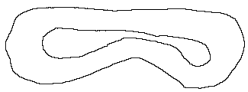
\includegraphics[interpolate=true,width=2.480000in,height=0.920000in]{contents/chapt7/figs/model/unknown_mass_path_1-img0.png}}%
\end{pgfscope}%
\begin{pgfscope}%
\pgfpathrectangle{\pgfqpoint{0.180000in}{1.566989in}}{\pgfqpoint{2.480000in}{0.915692in}}%
\pgfusepath{clip}%
\pgfsetrectcap%
\pgfsetroundjoin%
\pgfsetlinewidth{1.505625pt}%
\definecolor{currentstroke}{rgb}{0.121569,0.466667,0.705882}%
\pgfsetstrokecolor{currentstroke}%
\pgfsetstrokeopacity{0.700000}%
\pgfsetdash{}{0pt}%
\pgfpathmoveto{\pgfqpoint{1.706154in}{2.253758in}}%
\pgfpathlineto{\pgfqpoint{1.642249in}{2.254728in}}%
\pgfpathlineto{\pgfqpoint{1.580752in}{2.257988in}}%
\pgfpathlineto{\pgfqpoint{1.491262in}{2.265261in}}%
\pgfpathlineto{\pgfqpoint{1.357604in}{2.276476in}}%
\pgfpathlineto{\pgfqpoint{1.296317in}{2.279027in}}%
\pgfpathlineto{\pgfqpoint{1.204311in}{2.280252in}}%
\pgfpathlineto{\pgfqpoint{0.974282in}{2.281048in}}%
\pgfpathlineto{\pgfqpoint{0.912978in}{2.278909in}}%
\pgfpathlineto{\pgfqpoint{0.859437in}{2.275156in}}%
\pgfpathlineto{\pgfqpoint{0.806082in}{2.269333in}}%
\pgfpathlineto{\pgfqpoint{0.753009in}{2.261337in}}%
\pgfpathlineto{\pgfqpoint{0.700318in}{2.251126in}}%
\pgfpathlineto{\pgfqpoint{0.663089in}{2.241987in}}%
\pgfpathlineto{\pgfqpoint{0.633900in}{2.232589in}}%
\pgfpathlineto{\pgfqpoint{0.605640in}{2.220695in}}%
\pgfpathlineto{\pgfqpoint{0.585350in}{2.209869in}}%
\pgfpathlineto{\pgfqpoint{0.566113in}{2.197270in}}%
\pgfpathlineto{\pgfqpoint{0.548250in}{2.182792in}}%
\pgfpathlineto{\pgfqpoint{0.532189in}{2.166340in}}%
\pgfpathlineto{\pgfqpoint{0.518258in}{2.148051in}}%
\pgfpathlineto{\pgfqpoint{0.506815in}{2.128113in}}%
\pgfpathlineto{\pgfqpoint{0.498170in}{2.106813in}}%
\pgfpathlineto{\pgfqpoint{0.492601in}{2.084511in}}%
\pgfpathlineto{\pgfqpoint{0.490688in}{2.069300in}}%
\pgfpathlineto{\pgfqpoint{0.490533in}{2.046312in}}%
\pgfpathlineto{\pgfqpoint{0.493395in}{2.023501in}}%
\pgfpathlineto{\pgfqpoint{0.498983in}{2.001198in}}%
\pgfpathlineto{\pgfqpoint{0.507090in}{1.979682in}}%
\pgfpathlineto{\pgfqpoint{0.517428in}{1.959141in}}%
\pgfpathlineto{\pgfqpoint{0.529738in}{1.939718in}}%
\pgfpathlineto{\pgfqpoint{0.543776in}{1.921502in}}%
\pgfpathlineto{\pgfqpoint{0.559251in}{1.904489in}}%
\pgfpathlineto{\pgfqpoint{0.575952in}{1.888676in}}%
\pgfpathlineto{\pgfqpoint{0.599864in}{1.869482in}}%
\pgfpathlineto{\pgfqpoint{0.625341in}{1.852419in}}%
\pgfpathlineto{\pgfqpoint{0.652110in}{1.837462in}}%
\pgfpathlineto{\pgfqpoint{0.679960in}{1.824628in}}%
\pgfpathlineto{\pgfqpoint{0.708793in}{1.814194in}}%
\pgfpathlineto{\pgfqpoint{0.738429in}{1.806326in}}%
\pgfpathlineto{\pgfqpoint{0.768663in}{1.801225in}}%
\pgfpathlineto{\pgfqpoint{0.791583in}{1.799327in}}%
\pgfpathlineto{\pgfqpoint{0.814581in}{1.799132in}}%
\pgfpathlineto{\pgfqpoint{0.845167in}{1.801309in}}%
\pgfpathlineto{\pgfqpoint{0.875467in}{1.806021in}}%
\pgfpathlineto{\pgfqpoint{0.905313in}{1.813059in}}%
\pgfpathlineto{\pgfqpoint{0.934595in}{1.822171in}}%
\pgfpathlineto{\pgfqpoint{0.963228in}{1.833153in}}%
\pgfpathlineto{\pgfqpoint{0.998128in}{1.849014in}}%
\pgfpathlineto{\pgfqpoint{1.080421in}{1.890176in}}%
\pgfpathlineto{\pgfqpoint{1.129027in}{1.912940in}}%
\pgfpathlineto{\pgfqpoint{1.178569in}{1.933583in}}%
\pgfpathlineto{\pgfqpoint{1.229007in}{1.951932in}}%
\pgfpathlineto{\pgfqpoint{1.280202in}{1.968046in}}%
\pgfpathlineto{\pgfqpoint{1.332043in}{1.981943in}}%
\pgfpathlineto{\pgfqpoint{1.384425in}{1.993637in}}%
\pgfpathlineto{\pgfqpoint{1.422169in}{2.000349in}}%
\pgfpathlineto{\pgfqpoint{1.460220in}{2.005003in}}%
\pgfpathlineto{\pgfqpoint{1.498490in}{2.007174in}}%
\pgfpathlineto{\pgfqpoint{1.529155in}{2.006824in}}%
\pgfpathlineto{\pgfqpoint{1.559737in}{2.004531in}}%
\pgfpathlineto{\pgfqpoint{1.597728in}{1.999421in}}%
\pgfpathlineto{\pgfqpoint{1.635360in}{1.992109in}}%
\pgfpathlineto{\pgfqpoint{1.680009in}{1.981030in}}%
\pgfpathlineto{\pgfqpoint{1.723613in}{1.967801in}}%
\pgfpathlineto{\pgfqpoint{1.758507in}{1.954973in}}%
\pgfpathlineto{\pgfqpoint{1.791870in}{1.940287in}}%
\pgfpathlineto{\pgfqpoint{1.823460in}{1.923601in}}%
\pgfpathlineto{\pgfqpoint{1.852971in}{1.905061in}}%
\pgfpathlineto{\pgfqpoint{1.880257in}{1.884990in}}%
\pgfpathlineto{\pgfqpoint{1.905278in}{1.863636in}}%
\pgfpathlineto{\pgfqpoint{1.928054in}{1.841276in}}%
\pgfpathlineto{\pgfqpoint{1.958348in}{1.807654in}}%
\pgfpathlineto{\pgfqpoint{1.985717in}{1.778017in}}%
\pgfpathlineto{\pgfqpoint{2.010775in}{1.754001in}}%
\pgfpathlineto{\pgfqpoint{2.032691in}{1.735740in}}%
\pgfpathlineto{\pgfqpoint{2.056659in}{1.718762in}}%
\pgfpathlineto{\pgfqpoint{2.076143in}{1.707312in}}%
\pgfpathlineto{\pgfqpoint{2.096763in}{1.697301in}}%
\pgfpathlineto{\pgfqpoint{2.118190in}{1.689163in}}%
\pgfpathlineto{\pgfqpoint{2.140318in}{1.683193in}}%
\pgfpathlineto{\pgfqpoint{2.162940in}{1.679707in}}%
\pgfpathlineto{\pgfqpoint{2.185597in}{1.678874in}}%
\pgfpathlineto{\pgfqpoint{2.207943in}{1.680763in}}%
\pgfpathlineto{\pgfqpoint{2.229620in}{1.685457in}}%
\pgfpathlineto{\pgfqpoint{2.250241in}{1.692933in}}%
\pgfpathlineto{\pgfqpoint{2.269433in}{1.703037in}}%
\pgfpathlineto{\pgfqpoint{2.286843in}{1.715558in}}%
\pgfpathlineto{\pgfqpoint{2.302229in}{1.730256in}}%
\pgfpathlineto{\pgfqpoint{2.315575in}{1.746818in}}%
\pgfpathlineto{\pgfqpoint{2.327028in}{1.764734in}}%
\pgfpathlineto{\pgfqpoint{2.336748in}{1.783634in}}%
\pgfpathlineto{\pgfqpoint{2.347296in}{1.809914in}}%
\pgfpathlineto{\pgfqpoint{2.355482in}{1.837007in}}%
\pgfpathlineto{\pgfqpoint{2.361580in}{1.864649in}}%
\pgfpathlineto{\pgfqpoint{2.365417in}{1.892741in}}%
\pgfpathlineto{\pgfqpoint{2.366953in}{1.921098in}}%
\pgfpathlineto{\pgfqpoint{2.366052in}{1.949528in}}%
\pgfpathlineto{\pgfqpoint{2.362594in}{1.977806in}}%
\pgfpathlineto{\pgfqpoint{2.356447in}{2.005885in}}%
\pgfpathlineto{\pgfqpoint{2.347452in}{2.033822in}}%
\pgfpathlineto{\pgfqpoint{2.335667in}{2.061362in}}%
\pgfpathlineto{\pgfqpoint{2.321156in}{2.088214in}}%
\pgfpathlineto{\pgfqpoint{2.304162in}{2.113703in}}%
\pgfpathlineto{\pgfqpoint{2.289825in}{2.131662in}}%
\pgfpathlineto{\pgfqpoint{2.274192in}{2.148504in}}%
\pgfpathlineto{\pgfqpoint{2.257302in}{2.164085in}}%
\pgfpathlineto{\pgfqpoint{2.239244in}{2.178296in}}%
\pgfpathlineto{\pgfqpoint{2.220117in}{2.191032in}}%
\pgfpathlineto{\pgfqpoint{2.200047in}{2.202222in}}%
\pgfpathlineto{\pgfqpoint{2.179154in}{2.211790in}}%
\pgfpathlineto{\pgfqpoint{2.150304in}{2.222098in}}%
\pgfpathlineto{\pgfqpoint{2.120667in}{2.229862in}}%
\pgfpathlineto{\pgfqpoint{2.090500in}{2.235220in}}%
\pgfpathlineto{\pgfqpoint{2.060023in}{2.238380in}}%
\pgfpathlineto{\pgfqpoint{2.029403in}{2.239520in}}%
\pgfpathlineto{\pgfqpoint{1.991116in}{2.238455in}}%
\pgfpathlineto{\pgfqpoint{1.845792in}{2.230728in}}%
\pgfpathlineto{\pgfqpoint{1.807505in}{2.231854in}}%
\pgfpathlineto{\pgfqpoint{1.769330in}{2.234989in}}%
\pgfpathlineto{\pgfqpoint{1.731371in}{2.240112in}}%
\pgfpathlineto{\pgfqpoint{1.731371in}{2.240112in}}%
\pgfusepath{stroke}%
\end{pgfscope}%
\begin{pgfscope}%
\pgfpathrectangle{\pgfqpoint{0.180000in}{1.566989in}}{\pgfqpoint{2.480000in}{0.915692in}}%
\pgfusepath{clip}%
\pgfsetrectcap%
\pgfsetroundjoin%
\pgfsetlinewidth{1.505625pt}%
\definecolor{currentstroke}{rgb}{1.000000,0.498039,0.054902}%
\pgfsetstrokecolor{currentstroke}%
\pgfsetstrokeopacity{0.700000}%
\pgfsetdash{}{0pt}%
\pgfpathmoveto{\pgfqpoint{1.706154in}{2.253758in}}%
\pgfpathlineto{\pgfqpoint{1.642230in}{2.254741in}}%
\pgfpathlineto{\pgfqpoint{1.580687in}{2.258035in}}%
\pgfpathlineto{\pgfqpoint{1.491132in}{2.265448in}}%
\pgfpathlineto{\pgfqpoint{1.357242in}{2.276997in}}%
\pgfpathlineto{\pgfqpoint{1.295815in}{2.279739in}}%
\pgfpathlineto{\pgfqpoint{1.211276in}{2.281096in}}%
\pgfpathlineto{\pgfqpoint{0.973002in}{2.281763in}}%
\pgfpathlineto{\pgfqpoint{0.911552in}{2.279570in}}%
\pgfpathlineto{\pgfqpoint{0.857885in}{2.275754in}}%
\pgfpathlineto{\pgfqpoint{0.804412in}{2.269819in}}%
\pgfpathlineto{\pgfqpoint{0.751236in}{2.261636in}}%
\pgfpathlineto{\pgfqpoint{0.698466in}{2.251151in}}%
\pgfpathlineto{\pgfqpoint{0.661209in}{2.241744in}}%
\pgfpathlineto{\pgfqpoint{0.632036in}{2.232061in}}%
\pgfpathlineto{\pgfqpoint{0.610799in}{2.223089in}}%
\pgfpathlineto{\pgfqpoint{0.590358in}{2.212431in}}%
\pgfpathlineto{\pgfqpoint{0.570994in}{2.199925in}}%
\pgfpathlineto{\pgfqpoint{0.553039in}{2.185472in}}%
\pgfpathlineto{\pgfqpoint{0.536925in}{2.168996in}}%
\pgfpathlineto{\pgfqpoint{0.523057in}{2.150591in}}%
\pgfpathlineto{\pgfqpoint{0.511782in}{2.130495in}}%
\pgfpathlineto{\pgfqpoint{0.503443in}{2.109014in}}%
\pgfpathlineto{\pgfqpoint{0.499648in}{2.094122in}}%
\pgfpathlineto{\pgfqpoint{0.497339in}{2.078929in}}%
\pgfpathlineto{\pgfqpoint{0.496561in}{2.063580in}}%
\pgfpathlineto{\pgfqpoint{0.498231in}{2.040599in}}%
\pgfpathlineto{\pgfqpoint{0.503027in}{2.018059in}}%
\pgfpathlineto{\pgfqpoint{0.510580in}{1.996284in}}%
\pgfpathlineto{\pgfqpoint{0.520609in}{1.975532in}}%
\pgfpathlineto{\pgfqpoint{0.532818in}{1.955980in}}%
\pgfpathlineto{\pgfqpoint{0.546877in}{1.937712in}}%
\pgfpathlineto{\pgfqpoint{0.562512in}{1.920788in}}%
\pgfpathlineto{\pgfqpoint{0.585211in}{1.900332in}}%
\pgfpathlineto{\pgfqpoint{0.609538in}{1.882179in}}%
\pgfpathlineto{\pgfqpoint{0.635167in}{1.866299in}}%
\pgfpathlineto{\pgfqpoint{0.661803in}{1.852609in}}%
\pgfpathlineto{\pgfqpoint{0.689209in}{1.841022in}}%
\pgfpathlineto{\pgfqpoint{0.717359in}{1.831558in}}%
\pgfpathlineto{\pgfqpoint{0.746107in}{1.824200in}}%
\pgfpathlineto{\pgfqpoint{0.775292in}{1.818955in}}%
\pgfpathlineto{\pgfqpoint{0.804757in}{1.815851in}}%
\pgfpathlineto{\pgfqpoint{0.834450in}{1.814915in}}%
\pgfpathlineto{\pgfqpoint{0.865151in}{1.815991in}}%
\pgfpathlineto{\pgfqpoint{0.903487in}{1.819801in}}%
\pgfpathlineto{\pgfqpoint{0.941476in}{1.826204in}}%
\pgfpathlineto{\pgfqpoint{0.978939in}{1.835188in}}%
\pgfpathlineto{\pgfqpoint{1.015731in}{1.846620in}}%
\pgfpathlineto{\pgfqpoint{1.059178in}{1.862431in}}%
\pgfpathlineto{\pgfqpoint{1.123412in}{1.888588in}}%
\pgfpathlineto{\pgfqpoint{1.209091in}{1.923380in}}%
\pgfpathlineto{\pgfqpoint{1.267053in}{1.944375in}}%
\pgfpathlineto{\pgfqpoint{1.318485in}{1.960634in}}%
\pgfpathlineto{\pgfqpoint{1.370555in}{1.974716in}}%
\pgfpathlineto{\pgfqpoint{1.423189in}{1.986519in}}%
\pgfpathlineto{\pgfqpoint{1.461152in}{1.993088in}}%
\pgfpathlineto{\pgfqpoint{1.499427in}{1.997484in}}%
\pgfpathlineto{\pgfqpoint{1.530204in}{1.999138in}}%
\pgfpathlineto{\pgfqpoint{1.561024in}{1.998889in}}%
\pgfpathlineto{\pgfqpoint{1.591764in}{1.996649in}}%
\pgfpathlineto{\pgfqpoint{1.622318in}{1.992600in}}%
\pgfpathlineto{\pgfqpoint{1.660103in}{1.985083in}}%
\pgfpathlineto{\pgfqpoint{1.697315in}{1.975107in}}%
\pgfpathlineto{\pgfqpoint{1.733760in}{1.962948in}}%
\pgfpathlineto{\pgfqpoint{1.768634in}{1.948802in}}%
\pgfpathlineto{\pgfqpoint{1.801638in}{1.932655in}}%
\pgfpathlineto{\pgfqpoint{1.826515in}{1.918236in}}%
\pgfpathlineto{\pgfqpoint{1.849886in}{1.902487in}}%
\pgfpathlineto{\pgfqpoint{1.876821in}{1.881214in}}%
\pgfpathlineto{\pgfqpoint{1.901316in}{1.858712in}}%
\pgfpathlineto{\pgfqpoint{1.923436in}{1.835309in}}%
\pgfpathlineto{\pgfqpoint{1.947197in}{1.806512in}}%
\pgfpathlineto{\pgfqpoint{1.999345in}{1.739121in}}%
\pgfpathlineto{\pgfqpoint{2.018694in}{1.718921in}}%
\pgfpathlineto{\pgfqpoint{2.040277in}{1.700161in}}%
\pgfpathlineto{\pgfqpoint{2.057760in}{1.687900in}}%
\pgfpathlineto{\pgfqpoint{2.076374in}{1.677693in}}%
\pgfpathlineto{\pgfqpoint{2.095993in}{1.669918in}}%
\pgfpathlineto{\pgfqpoint{2.116370in}{1.664931in}}%
\pgfpathlineto{\pgfqpoint{2.137138in}{1.663045in}}%
\pgfpathlineto{\pgfqpoint{2.150968in}{1.663601in}}%
\pgfpathlineto{\pgfqpoint{2.164613in}{1.665640in}}%
\pgfpathlineto{\pgfqpoint{2.184451in}{1.671401in}}%
\pgfpathlineto{\pgfqpoint{2.203193in}{1.680023in}}%
\pgfpathlineto{\pgfqpoint{2.220615in}{1.691022in}}%
\pgfpathlineto{\pgfqpoint{2.236643in}{1.703921in}}%
\pgfpathlineto{\pgfqpoint{2.251222in}{1.718396in}}%
\pgfpathlineto{\pgfqpoint{2.264406in}{1.734114in}}%
\pgfpathlineto{\pgfqpoint{2.279909in}{1.756375in}}%
\pgfpathlineto{\pgfqpoint{2.296796in}{1.784927in}}%
\pgfpathlineto{\pgfqpoint{2.328608in}{1.840309in}}%
\pgfpathlineto{\pgfqpoint{2.342739in}{1.860878in}}%
\pgfpathlineto{\pgfqpoint{2.363311in}{1.886437in}}%
\pgfpathlineto{\pgfqpoint{2.434147in}{1.969684in}}%
\pgfpathlineto{\pgfqpoint{2.449752in}{1.993873in}}%
\pgfpathlineto{\pgfqpoint{2.459369in}{2.012009in}}%
\pgfpathlineto{\pgfqpoint{2.466775in}{2.030170in}}%
\pgfpathlineto{\pgfqpoint{2.471717in}{2.048204in}}%
\pgfpathlineto{\pgfqpoint{2.474030in}{2.065839in}}%
\pgfpathlineto{\pgfqpoint{2.473649in}{2.082865in}}%
\pgfpathlineto{\pgfqpoint{2.470272in}{2.099936in}}%
\pgfpathlineto{\pgfqpoint{2.464228in}{2.116825in}}%
\pgfpathlineto{\pgfqpoint{2.455967in}{2.133347in}}%
\pgfpathlineto{\pgfqpoint{2.445804in}{2.149407in}}%
\pgfpathlineto{\pgfqpoint{2.433902in}{2.164898in}}%
\pgfpathlineto{\pgfqpoint{2.420319in}{2.179669in}}%
\pgfpathlineto{\pgfqpoint{2.405097in}{2.193565in}}%
\pgfpathlineto{\pgfqpoint{2.382452in}{2.210654in}}%
\pgfpathlineto{\pgfqpoint{2.357414in}{2.226040in}}%
\pgfpathlineto{\pgfqpoint{2.330232in}{2.239524in}}%
\pgfpathlineto{\pgfqpoint{2.301780in}{2.250605in}}%
\pgfpathlineto{\pgfqpoint{2.272413in}{2.258954in}}%
\pgfpathlineto{\pgfqpoint{2.242396in}{2.264548in}}%
\pgfpathlineto{\pgfqpoint{2.212031in}{2.267783in}}%
\pgfpathlineto{\pgfqpoint{2.181513in}{2.268875in}}%
\pgfpathlineto{\pgfqpoint{2.143358in}{2.267735in}}%
\pgfpathlineto{\pgfqpoint{2.097777in}{2.263752in}}%
\pgfpathlineto{\pgfqpoint{2.022124in}{2.256948in}}%
\pgfpathlineto{\pgfqpoint{1.984307in}{2.255741in}}%
\pgfpathlineto{\pgfqpoint{1.946105in}{2.256792in}}%
\pgfpathlineto{\pgfqpoint{1.900393in}{2.260442in}}%
\pgfpathlineto{\pgfqpoint{1.847335in}{2.267334in}}%
\pgfpathlineto{\pgfqpoint{1.726299in}{2.284766in}}%
\pgfpathlineto{\pgfqpoint{1.703451in}{2.286725in}}%
\pgfpathlineto{\pgfqpoint{1.703451in}{2.286725in}}%
\pgfusepath{stroke}%
\end{pgfscope}%
\begin{pgfscope}%
\definecolor{textcolor}{rgb}{0.000000,0.000000,0.000000}%
\pgfsetstrokecolor{textcolor}%
\pgfsetfillcolor{textcolor}%
\pgftext[x=1.420000in,y=2.566015in,,base]{\color{textcolor}\rmfamily\fontsize{12.000000}{14.400000}\selectfont End-to-end}%
\end{pgfscope}%
\begin{pgfscope}%
\pgfpathrectangle{\pgfqpoint{2.840000in}{1.566989in}}{\pgfqpoint{2.480000in}{0.915692in}}%
\pgfusepath{clip}%
\pgfsys@transformshift{2.840000in}{1.566989in}%
\pgftext[left,bottom]{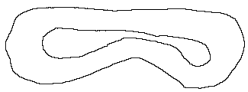
\includegraphics[interpolate=true,width=2.480000in,height=0.920000in]{contents/chapt7/figs/model/unknown_mass_path_1-img1.png}}%
\end{pgfscope}%
\begin{pgfscope}%
\pgfpathrectangle{\pgfqpoint{2.840000in}{1.566989in}}{\pgfqpoint{2.480000in}{0.915692in}}%
\pgfusepath{clip}%
\pgfsetrectcap%
\pgfsetroundjoin%
\pgfsetlinewidth{1.505625pt}%
\definecolor{currentstroke}{rgb}{0.121569,0.466667,0.705882}%
\pgfsetstrokecolor{currentstroke}%
\pgfsetstrokeopacity{0.700000}%
\pgfsetdash{}{0pt}%
\pgfpathmoveto{\pgfqpoint{4.366154in}{2.253758in}}%
\pgfpathlineto{\pgfqpoint{4.313854in}{2.254695in}}%
\pgfpathlineto{\pgfqpoint{4.275631in}{2.257832in}}%
\pgfpathlineto{\pgfqpoint{4.232535in}{2.263794in}}%
\pgfpathlineto{\pgfqpoint{4.096952in}{2.285781in}}%
\pgfpathlineto{\pgfqpoint{4.058886in}{2.288462in}}%
\pgfpathlineto{\pgfqpoint{4.013101in}{2.289410in}}%
\pgfpathlineto{\pgfqpoint{3.952051in}{2.288233in}}%
\pgfpathlineto{\pgfqpoint{3.814718in}{2.284435in}}%
\pgfpathlineto{\pgfqpoint{3.753667in}{2.285530in}}%
\pgfpathlineto{\pgfqpoint{3.608705in}{2.289510in}}%
\pgfpathlineto{\pgfqpoint{3.562938in}{2.287970in}}%
\pgfpathlineto{\pgfqpoint{3.524926in}{2.284612in}}%
\pgfpathlineto{\pgfqpoint{3.487165in}{2.279101in}}%
\pgfpathlineto{\pgfqpoint{3.442295in}{2.269951in}}%
\pgfpathlineto{\pgfqpoint{3.390489in}{2.256890in}}%
\pgfpathlineto{\pgfqpoint{3.339246in}{2.241768in}}%
\pgfpathlineto{\pgfqpoint{3.295966in}{2.226807in}}%
\pgfpathlineto{\pgfqpoint{3.260798in}{2.212005in}}%
\pgfpathlineto{\pgfqpoint{3.233711in}{2.197935in}}%
\pgfpathlineto{\pgfqpoint{3.214322in}{2.185761in}}%
\pgfpathlineto{\pgfqpoint{3.196024in}{2.172005in}}%
\pgfpathlineto{\pgfqpoint{3.179094in}{2.156597in}}%
\pgfpathlineto{\pgfqpoint{3.163764in}{2.139599in}}%
\pgfpathlineto{\pgfqpoint{3.150367in}{2.121040in}}%
\pgfpathlineto{\pgfqpoint{3.139232in}{2.101044in}}%
\pgfpathlineto{\pgfqpoint{3.130602in}{2.079848in}}%
\pgfpathlineto{\pgfqpoint{3.124707in}{2.057735in}}%
\pgfpathlineto{\pgfqpoint{3.121712in}{2.035047in}}%
\pgfpathlineto{\pgfqpoint{3.121577in}{2.012161in}}%
\pgfpathlineto{\pgfqpoint{3.124111in}{1.989414in}}%
\pgfpathlineto{\pgfqpoint{3.129231in}{1.967105in}}%
\pgfpathlineto{\pgfqpoint{3.136839in}{1.945518in}}%
\pgfpathlineto{\pgfqpoint{3.146828in}{1.924924in}}%
\pgfpathlineto{\pgfqpoint{3.159043in}{1.905569in}}%
\pgfpathlineto{\pgfqpoint{3.173388in}{1.887733in}}%
\pgfpathlineto{\pgfqpoint{3.189586in}{1.871561in}}%
\pgfpathlineto{\pgfqpoint{3.207385in}{1.857168in}}%
\pgfpathlineto{\pgfqpoint{3.226588in}{1.844711in}}%
\pgfpathlineto{\pgfqpoint{3.246993in}{1.834338in}}%
\pgfpathlineto{\pgfqpoint{3.268351in}{1.826104in}}%
\pgfpathlineto{\pgfqpoint{3.290413in}{1.819997in}}%
\pgfpathlineto{\pgfqpoint{3.312949in}{1.815971in}}%
\pgfpathlineto{\pgfqpoint{3.335736in}{1.813767in}}%
\pgfpathlineto{\pgfqpoint{3.366257in}{1.813334in}}%
\pgfpathlineto{\pgfqpoint{3.396715in}{1.815356in}}%
\pgfpathlineto{\pgfqpoint{3.426959in}{1.819503in}}%
\pgfpathlineto{\pgfqpoint{3.464324in}{1.827246in}}%
\pgfpathlineto{\pgfqpoint{3.508583in}{1.839002in}}%
\pgfpathlineto{\pgfqpoint{3.596185in}{1.865754in}}%
\pgfpathlineto{\pgfqpoint{3.647638in}{1.880134in}}%
\pgfpathlineto{\pgfqpoint{3.684900in}{1.888371in}}%
\pgfpathlineto{\pgfqpoint{3.722563in}{1.894507in}}%
\pgfpathlineto{\pgfqpoint{3.760513in}{1.898518in}}%
\pgfpathlineto{\pgfqpoint{3.821457in}{1.902297in}}%
\pgfpathlineto{\pgfqpoint{3.897648in}{1.906850in}}%
\pgfpathlineto{\pgfqpoint{3.943184in}{1.911699in}}%
\pgfpathlineto{\pgfqpoint{3.995992in}{1.919810in}}%
\pgfpathlineto{\pgfqpoint{4.116500in}{1.939549in}}%
\pgfpathlineto{\pgfqpoint{4.154491in}{1.943133in}}%
\pgfpathlineto{\pgfqpoint{4.185001in}{1.944195in}}%
\pgfpathlineto{\pgfqpoint{4.215514in}{1.943292in}}%
\pgfpathlineto{\pgfqpoint{4.245884in}{1.940211in}}%
\pgfpathlineto{\pgfqpoint{4.275946in}{1.934914in}}%
\pgfpathlineto{\pgfqpoint{4.305538in}{1.927417in}}%
\pgfpathlineto{\pgfqpoint{4.334551in}{1.917924in}}%
\pgfpathlineto{\pgfqpoint{4.369990in}{1.903771in}}%
\pgfpathlineto{\pgfqpoint{4.418672in}{1.881756in}}%
\pgfpathlineto{\pgfqpoint{4.584922in}{1.804822in}}%
\pgfpathlineto{\pgfqpoint{4.682715in}{1.761760in}}%
\pgfpathlineto{\pgfqpoint{4.711380in}{1.751258in}}%
\pgfpathlineto{\pgfqpoint{4.740706in}{1.742791in}}%
\pgfpathlineto{\pgfqpoint{4.763144in}{1.738245in}}%
\pgfpathlineto{\pgfqpoint{4.785781in}{1.735553in}}%
\pgfpathlineto{\pgfqpoint{4.808415in}{1.734709in}}%
\pgfpathlineto{\pgfqpoint{4.830894in}{1.735750in}}%
\pgfpathlineto{\pgfqpoint{4.853055in}{1.738701in}}%
\pgfpathlineto{\pgfqpoint{4.874728in}{1.743560in}}%
\pgfpathlineto{\pgfqpoint{4.895730in}{1.750319in}}%
\pgfpathlineto{\pgfqpoint{4.915986in}{1.758971in}}%
\pgfpathlineto{\pgfqpoint{4.936069in}{1.769673in}}%
\pgfpathlineto{\pgfqpoint{4.955536in}{1.781985in}}%
\pgfpathlineto{\pgfqpoint{4.974037in}{1.795707in}}%
\pgfpathlineto{\pgfqpoint{4.991411in}{1.810828in}}%
\pgfpathlineto{\pgfqpoint{5.007439in}{1.827369in}}%
\pgfpathlineto{\pgfqpoint{5.021891in}{1.845301in}}%
\pgfpathlineto{\pgfqpoint{5.034540in}{1.864547in}}%
\pgfpathlineto{\pgfqpoint{5.045295in}{1.884913in}}%
\pgfpathlineto{\pgfqpoint{5.054110in}{1.906191in}}%
\pgfpathlineto{\pgfqpoint{5.060900in}{1.928199in}}%
\pgfpathlineto{\pgfqpoint{5.065563in}{1.950752in}}%
\pgfpathlineto{\pgfqpoint{5.068012in}{1.973652in}}%
\pgfpathlineto{\pgfqpoint{5.068158in}{1.996682in}}%
\pgfpathlineto{\pgfqpoint{5.065976in}{2.019609in}}%
\pgfpathlineto{\pgfqpoint{5.061501in}{2.042200in}}%
\pgfpathlineto{\pgfqpoint{5.054745in}{2.064217in}}%
\pgfpathlineto{\pgfqpoint{5.045750in}{2.085417in}}%
\pgfpathlineto{\pgfqpoint{5.034622in}{2.105581in}}%
\pgfpathlineto{\pgfqpoint{5.021471in}{2.124486in}}%
\pgfpathlineto{\pgfqpoint{5.006380in}{2.141882in}}%
\pgfpathlineto{\pgfqpoint{4.989561in}{2.157615in}}%
\pgfpathlineto{\pgfqpoint{4.971340in}{2.171702in}}%
\pgfpathlineto{\pgfqpoint{4.951923in}{2.184090in}}%
\pgfpathlineto{\pgfqpoint{4.931549in}{2.194834in}}%
\pgfpathlineto{\pgfqpoint{4.910408in}{2.203980in}}%
\pgfpathlineto{\pgfqpoint{4.881349in}{2.213915in}}%
\pgfpathlineto{\pgfqpoint{4.844181in}{2.223530in}}%
\pgfpathlineto{\pgfqpoint{4.798983in}{2.232472in}}%
\pgfpathlineto{\pgfqpoint{4.738302in}{2.242061in}}%
\pgfpathlineto{\pgfqpoint{4.555717in}{2.267147in}}%
\pgfpathlineto{\pgfqpoint{4.517432in}{2.270044in}}%
\pgfpathlineto{\pgfqpoint{4.479047in}{2.270880in}}%
\pgfpathlineto{\pgfqpoint{4.433000in}{2.269367in}}%
\pgfpathlineto{\pgfqpoint{4.433000in}{2.269367in}}%
\pgfusepath{stroke}%
\end{pgfscope}%
\begin{pgfscope}%
\pgfpathrectangle{\pgfqpoint{2.840000in}{1.566989in}}{\pgfqpoint{2.480000in}{0.915692in}}%
\pgfusepath{clip}%
\pgfsetrectcap%
\pgfsetroundjoin%
\pgfsetlinewidth{1.505625pt}%
\definecolor{currentstroke}{rgb}{1.000000,0.498039,0.054902}%
\pgfsetstrokecolor{currentstroke}%
\pgfsetstrokeopacity{0.700000}%
\pgfsetdash{}{0pt}%
\pgfpathmoveto{\pgfqpoint{4.366154in}{2.253758in}}%
\pgfpathlineto{\pgfqpoint{4.313854in}{2.254709in}}%
\pgfpathlineto{\pgfqpoint{4.275632in}{2.257848in}}%
\pgfpathlineto{\pgfqpoint{4.232526in}{2.263809in}}%
\pgfpathlineto{\pgfqpoint{4.157257in}{2.277510in}}%
\pgfpathlineto{\pgfqpoint{4.096896in}{2.287619in}}%
\pgfpathlineto{\pgfqpoint{4.051303in}{2.292920in}}%
\pgfpathlineto{\pgfqpoint{3.997904in}{2.296969in}}%
\pgfpathlineto{\pgfqpoint{3.936750in}{2.299400in}}%
\pgfpathlineto{\pgfqpoint{3.867897in}{2.299713in}}%
\pgfpathlineto{\pgfqpoint{3.776122in}{2.297277in}}%
\pgfpathlineto{\pgfqpoint{3.691981in}{2.295791in}}%
\pgfpathlineto{\pgfqpoint{3.615484in}{2.296939in}}%
\pgfpathlineto{\pgfqpoint{3.554285in}{2.297431in}}%
\pgfpathlineto{\pgfqpoint{3.516068in}{2.295837in}}%
\pgfpathlineto{\pgfqpoint{3.478026in}{2.291893in}}%
\pgfpathlineto{\pgfqpoint{3.440335in}{2.285388in}}%
\pgfpathlineto{\pgfqpoint{3.395592in}{2.275153in}}%
\pgfpathlineto{\pgfqpoint{3.351449in}{2.262574in}}%
\pgfpathlineto{\pgfqpoint{3.315208in}{2.250339in}}%
\pgfpathlineto{\pgfqpoint{3.279727in}{2.236058in}}%
\pgfpathlineto{\pgfqpoint{3.252220in}{2.222661in}}%
\pgfpathlineto{\pgfqpoint{3.225903in}{2.207062in}}%
\pgfpathlineto{\pgfqpoint{3.207271in}{2.193668in}}%
\pgfpathlineto{\pgfqpoint{3.189901in}{2.178677in}}%
\pgfpathlineto{\pgfqpoint{3.174024in}{2.162114in}}%
\pgfpathlineto{\pgfqpoint{3.159913in}{2.144024in}}%
\pgfpathlineto{\pgfqpoint{3.147898in}{2.124480in}}%
\pgfpathlineto{\pgfqpoint{3.138223in}{2.103680in}}%
\pgfpathlineto{\pgfqpoint{3.131113in}{2.081870in}}%
\pgfpathlineto{\pgfqpoint{3.126731in}{2.059353in}}%
\pgfpathlineto{\pgfqpoint{3.125118in}{2.036470in}}%
\pgfpathlineto{\pgfqpoint{3.126155in}{2.013552in}}%
\pgfpathlineto{\pgfqpoint{3.129517in}{1.990854in}}%
\pgfpathlineto{\pgfqpoint{3.135029in}{1.968582in}}%
\pgfpathlineto{\pgfqpoint{3.142618in}{1.946929in}}%
\pgfpathlineto{\pgfqpoint{3.152250in}{1.926104in}}%
\pgfpathlineto{\pgfqpoint{3.163860in}{1.906315in}}%
\pgfpathlineto{\pgfqpoint{3.177386in}{1.887782in}}%
\pgfpathlineto{\pgfqpoint{3.192774in}{1.870766in}}%
\pgfpathlineto{\pgfqpoint{3.209931in}{1.855536in}}%
\pgfpathlineto{\pgfqpoint{3.228726in}{1.842383in}}%
\pgfpathlineto{\pgfqpoint{3.248929in}{1.831514in}}%
\pgfpathlineto{\pgfqpoint{3.270254in}{1.823058in}}%
\pgfpathlineto{\pgfqpoint{3.292400in}{1.817067in}}%
\pgfpathlineto{\pgfqpoint{3.315062in}{1.813480in}}%
\pgfpathlineto{\pgfqpoint{3.337959in}{1.811987in}}%
\pgfpathlineto{\pgfqpoint{3.368549in}{1.812551in}}%
\pgfpathlineto{\pgfqpoint{3.399016in}{1.815379in}}%
\pgfpathlineto{\pgfqpoint{3.436790in}{1.821378in}}%
\pgfpathlineto{\pgfqpoint{3.489145in}{1.832634in}}%
\pgfpathlineto{\pgfqpoint{3.548440in}{1.847796in}}%
\pgfpathlineto{\pgfqpoint{3.666763in}{1.879102in}}%
\pgfpathlineto{\pgfqpoint{3.704334in}{1.886277in}}%
\pgfpathlineto{\pgfqpoint{3.742228in}{1.891476in}}%
\pgfpathlineto{\pgfqpoint{3.795570in}{1.896222in}}%
\pgfpathlineto{\pgfqpoint{3.894661in}{1.904689in}}%
\pgfpathlineto{\pgfqpoint{3.955348in}{1.912624in}}%
\pgfpathlineto{\pgfqpoint{4.106839in}{1.934059in}}%
\pgfpathlineto{\pgfqpoint{4.152579in}{1.937880in}}%
\pgfpathlineto{\pgfqpoint{4.190814in}{1.938867in}}%
\pgfpathlineto{\pgfqpoint{4.221391in}{1.937730in}}%
\pgfpathlineto{\pgfqpoint{4.251824in}{1.934563in}}%
\pgfpathlineto{\pgfqpoint{4.281950in}{1.929217in}}%
\pgfpathlineto{\pgfqpoint{4.311625in}{1.921764in}}%
\pgfpathlineto{\pgfqpoint{4.340732in}{1.912328in}}%
\pgfpathlineto{\pgfqpoint{4.376280in}{1.898210in}}%
\pgfpathlineto{\pgfqpoint{4.446162in}{1.867071in}}%
\pgfpathlineto{\pgfqpoint{4.537174in}{1.826971in}}%
\pgfpathlineto{\pgfqpoint{4.636484in}{1.786848in}}%
\pgfpathlineto{\pgfqpoint{4.700891in}{1.762518in}}%
\pgfpathlineto{\pgfqpoint{4.730119in}{1.753463in}}%
\pgfpathlineto{\pgfqpoint{4.759938in}{1.746617in}}%
\pgfpathlineto{\pgfqpoint{4.782607in}{1.743410in}}%
\pgfpathlineto{\pgfqpoint{4.805310in}{1.742083in}}%
\pgfpathlineto{\pgfqpoint{4.827888in}{1.742662in}}%
\pgfpathlineto{\pgfqpoint{4.850161in}{1.745322in}}%
\pgfpathlineto{\pgfqpoint{4.871923in}{1.750085in}}%
\pgfpathlineto{\pgfqpoint{4.892965in}{1.756914in}}%
\pgfpathlineto{\pgfqpoint{4.913102in}{1.765696in}}%
\pgfpathlineto{\pgfqpoint{4.932761in}{1.776617in}}%
\pgfpathlineto{\pgfqpoint{4.951958in}{1.789393in}}%
\pgfpathlineto{\pgfqpoint{4.970121in}{1.803602in}}%
\pgfpathlineto{\pgfqpoint{4.987110in}{1.819194in}}%
\pgfpathlineto{\pgfqpoint{5.002743in}{1.836145in}}%
\pgfpathlineto{\pgfqpoint{5.016807in}{1.854417in}}%
\pgfpathlineto{\pgfqpoint{5.029068in}{1.873944in}}%
\pgfpathlineto{\pgfqpoint{5.039403in}{1.894555in}}%
\pgfpathlineto{\pgfqpoint{5.047681in}{1.916075in}}%
\pgfpathlineto{\pgfqpoint{5.053767in}{1.938314in}}%
\pgfpathlineto{\pgfqpoint{5.057594in}{1.961050in}}%
\pgfpathlineto{\pgfqpoint{5.059066in}{1.984059in}}%
\pgfpathlineto{\pgfqpoint{5.058121in}{2.007095in}}%
\pgfpathlineto{\pgfqpoint{5.054733in}{2.029901in}}%
\pgfpathlineto{\pgfqpoint{5.049150in}{2.052273in}}%
\pgfpathlineto{\pgfqpoint{5.041524in}{2.074034in}}%
\pgfpathlineto{\pgfqpoint{5.031879in}{2.094978in}}%
\pgfpathlineto{\pgfqpoint{5.020290in}{2.114911in}}%
\pgfpathlineto{\pgfqpoint{5.006892in}{2.133677in}}%
\pgfpathlineto{\pgfqpoint{4.991762in}{2.151075in}}%
\pgfpathlineto{\pgfqpoint{4.975040in}{2.166952in}}%
\pgfpathlineto{\pgfqpoint{4.956995in}{2.181308in}}%
\pgfpathlineto{\pgfqpoint{4.937790in}{2.194070in}}%
\pgfpathlineto{\pgfqpoint{4.917587in}{2.205189in}}%
\pgfpathlineto{\pgfqpoint{4.896590in}{2.214723in}}%
\pgfpathlineto{\pgfqpoint{4.867657in}{2.225119in}}%
\pgfpathlineto{\pgfqpoint{4.837970in}{2.233128in}}%
\pgfpathlineto{\pgfqpoint{4.792775in}{2.242348in}}%
\pgfpathlineto{\pgfqpoint{4.732066in}{2.252209in}}%
\pgfpathlineto{\pgfqpoint{4.610264in}{2.269430in}}%
\pgfpathlineto{\pgfqpoint{4.556753in}{2.275147in}}%
\pgfpathlineto{\pgfqpoint{4.510712in}{2.277940in}}%
\pgfpathlineto{\pgfqpoint{4.464588in}{2.278332in}}%
\pgfpathlineto{\pgfqpoint{4.410818in}{2.276140in}}%
\pgfpathlineto{\pgfqpoint{4.410818in}{2.276140in}}%
\pgfusepath{stroke}%
\end{pgfscope}%
\begin{pgfscope}%
\definecolor{textcolor}{rgb}{0.000000,0.000000,0.000000}%
\pgfsetstrokecolor{textcolor}%
\pgfsetfillcolor{textcolor}%
\pgftext[x=4.080000in,y=2.566015in,,base]{\color{textcolor}\rmfamily\fontsize{12.000000}{14.400000}\selectfont Steering controller}%
\end{pgfscope}%
\begin{pgfscope}%
\pgfpathrectangle{\pgfqpoint{0.180000in}{0.404960in}}{\pgfqpoint{2.480000in}{0.915692in}}%
\pgfusepath{clip}%
\pgfsys@transformshift{0.180000in}{0.404960in}%
\pgftext[left,bottom]{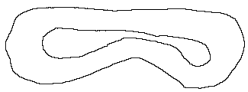
\includegraphics[interpolate=true,width=2.480000in,height=0.920000in]{contents/chapt7/figs/model/unknown_mass_path_1-img2.png}}%
\end{pgfscope}%
\begin{pgfscope}%
\pgfpathrectangle{\pgfqpoint{0.180000in}{0.404960in}}{\pgfqpoint{2.480000in}{0.915692in}}%
\pgfusepath{clip}%
\pgfsetrectcap%
\pgfsetroundjoin%
\pgfsetlinewidth{1.505625pt}%
\definecolor{currentstroke}{rgb}{0.121569,0.466667,0.705882}%
\pgfsetstrokecolor{currentstroke}%
\pgfsetstrokeopacity{0.700000}%
\pgfsetdash{}{0pt}%
\pgfpathmoveto{\pgfqpoint{1.706154in}{1.091729in}}%
\pgfpathlineto{\pgfqpoint{1.630646in}{1.092754in}}%
\pgfpathlineto{\pgfqpoint{1.566764in}{1.095756in}}%
\pgfpathlineto{\pgfqpoint{1.387983in}{1.105496in}}%
\pgfpathlineto{\pgfqpoint{1.332672in}{1.105957in}}%
\pgfpathlineto{\pgfqpoint{1.270900in}{1.104072in}}%
\pgfpathlineto{\pgfqpoint{1.170407in}{1.101112in}}%
\pgfpathlineto{\pgfqpoint{1.057964in}{1.101870in}}%
\pgfpathlineto{\pgfqpoint{0.977468in}{1.101402in}}%
\pgfpathlineto{\pgfqpoint{0.915600in}{1.098637in}}%
\pgfpathlineto{\pgfqpoint{0.873584in}{1.095024in}}%
\pgfpathlineto{\pgfqpoint{0.831012in}{1.088878in}}%
\pgfpathlineto{\pgfqpoint{0.795453in}{1.081352in}}%
\pgfpathlineto{\pgfqpoint{0.760346in}{1.071348in}}%
\pgfpathlineto{\pgfqpoint{0.732678in}{1.061218in}}%
\pgfpathlineto{\pgfqpoint{0.705653in}{1.048802in}}%
\pgfpathlineto{\pgfqpoint{0.679760in}{1.034071in}}%
\pgfpathlineto{\pgfqpoint{0.661278in}{1.021416in}}%
\pgfpathlineto{\pgfqpoint{0.643773in}{1.007348in}}%
\pgfpathlineto{\pgfqpoint{0.627443in}{0.991915in}}%
\pgfpathlineto{\pgfqpoint{0.612600in}{0.974997in}}%
\pgfpathlineto{\pgfqpoint{0.599606in}{0.956560in}}%
\pgfpathlineto{\pgfqpoint{0.588729in}{0.936746in}}%
\pgfpathlineto{\pgfqpoint{0.580274in}{0.915714in}}%
\pgfpathlineto{\pgfqpoint{0.574523in}{0.893750in}}%
\pgfpathlineto{\pgfqpoint{0.571699in}{0.871117in}}%
\pgfpathlineto{\pgfqpoint{0.571859in}{0.848220in}}%
\pgfpathlineto{\pgfqpoint{0.574938in}{0.825554in}}%
\pgfpathlineto{\pgfqpoint{0.580916in}{0.803457in}}%
\pgfpathlineto{\pgfqpoint{0.589693in}{0.782327in}}%
\pgfpathlineto{\pgfqpoint{0.601087in}{0.762526in}}%
\pgfpathlineto{\pgfqpoint{0.614925in}{0.744367in}}%
\pgfpathlineto{\pgfqpoint{0.630966in}{0.728135in}}%
\pgfpathlineto{\pgfqpoint{0.648686in}{0.714086in}}%
\pgfpathlineto{\pgfqpoint{0.667669in}{0.702206in}}%
\pgfpathlineto{\pgfqpoint{0.687681in}{0.692543in}}%
\pgfpathlineto{\pgfqpoint{0.708441in}{0.685105in}}%
\pgfpathlineto{\pgfqpoint{0.729722in}{0.679788in}}%
\pgfpathlineto{\pgfqpoint{0.751287in}{0.676489in}}%
\pgfpathlineto{\pgfqpoint{0.772946in}{0.675075in}}%
\pgfpathlineto{\pgfqpoint{0.801820in}{0.675643in}}%
\pgfpathlineto{\pgfqpoint{0.837795in}{0.679049in}}%
\pgfpathlineto{\pgfqpoint{0.880600in}{0.685531in}}%
\pgfpathlineto{\pgfqpoint{0.959093in}{0.700091in}}%
\pgfpathlineto{\pgfqpoint{1.060261in}{0.721003in}}%
\pgfpathlineto{\pgfqpoint{1.125826in}{0.736476in}}%
\pgfpathlineto{\pgfqpoint{1.183896in}{0.752400in}}%
\pgfpathlineto{\pgfqpoint{1.350397in}{0.801107in}}%
\pgfpathlineto{\pgfqpoint{1.394242in}{0.810030in}}%
\pgfpathlineto{\pgfqpoint{1.430863in}{0.815478in}}%
\pgfpathlineto{\pgfqpoint{1.467487in}{0.819021in}}%
\pgfpathlineto{\pgfqpoint{1.503841in}{0.820619in}}%
\pgfpathlineto{\pgfqpoint{1.539354in}{0.819802in}}%
\pgfpathlineto{\pgfqpoint{1.567114in}{0.817218in}}%
\pgfpathlineto{\pgfqpoint{1.594204in}{0.812777in}}%
\pgfpathlineto{\pgfqpoint{1.620539in}{0.806409in}}%
\pgfpathlineto{\pgfqpoint{1.653372in}{0.795718in}}%
\pgfpathlineto{\pgfqpoint{1.699928in}{0.777786in}}%
\pgfpathlineto{\pgfqpoint{1.814428in}{0.730177in}}%
\pgfpathlineto{\pgfqpoint{1.874225in}{0.703106in}}%
\pgfpathlineto{\pgfqpoint{1.932881in}{0.673809in}}%
\pgfpathlineto{\pgfqpoint{2.076756in}{0.600729in}}%
\pgfpathlineto{\pgfqpoint{2.104520in}{0.589967in}}%
\pgfpathlineto{\pgfqpoint{2.126031in}{0.583765in}}%
\pgfpathlineto{\pgfqpoint{2.148159in}{0.579621in}}%
\pgfpathlineto{\pgfqpoint{2.170717in}{0.577902in}}%
\pgfpathlineto{\pgfqpoint{2.193283in}{0.578949in}}%
\pgfpathlineto{\pgfqpoint{2.215460in}{0.582983in}}%
\pgfpathlineto{\pgfqpoint{2.236794in}{0.590147in}}%
\pgfpathlineto{\pgfqpoint{2.250329in}{0.596670in}}%
\pgfpathlineto{\pgfqpoint{2.263108in}{0.604532in}}%
\pgfpathlineto{\pgfqpoint{2.275032in}{0.613704in}}%
\pgfpathlineto{\pgfqpoint{2.285919in}{0.624055in}}%
\pgfpathlineto{\pgfqpoint{2.295653in}{0.635486in}}%
\pgfpathlineto{\pgfqpoint{2.304157in}{0.647887in}}%
\pgfpathlineto{\pgfqpoint{2.314570in}{0.667912in}}%
\pgfpathlineto{\pgfqpoint{2.322101in}{0.689230in}}%
\pgfpathlineto{\pgfqpoint{2.326711in}{0.711384in}}%
\pgfpathlineto{\pgfqpoint{2.328446in}{0.734024in}}%
\pgfpathlineto{\pgfqpoint{2.327411in}{0.756730in}}%
\pgfpathlineto{\pgfqpoint{2.323698in}{0.779219in}}%
\pgfpathlineto{\pgfqpoint{2.317518in}{0.801142in}}%
\pgfpathlineto{\pgfqpoint{2.309232in}{0.822362in}}%
\pgfpathlineto{\pgfqpoint{2.299096in}{0.842749in}}%
\pgfpathlineto{\pgfqpoint{2.287283in}{0.862267in}}%
\pgfpathlineto{\pgfqpoint{2.269304in}{0.886855in}}%
\pgfpathlineto{\pgfqpoint{2.249199in}{0.909783in}}%
\pgfpathlineto{\pgfqpoint{2.227710in}{0.930948in}}%
\pgfpathlineto{\pgfqpoint{2.205142in}{0.950395in}}%
\pgfpathlineto{\pgfqpoint{2.175575in}{0.972470in}}%
\pgfpathlineto{\pgfqpoint{2.144748in}{0.992294in}}%
\pgfpathlineto{\pgfqpoint{2.112680in}{1.010090in}}%
\pgfpathlineto{\pgfqpoint{2.085781in}{1.022763in}}%
\pgfpathlineto{\pgfqpoint{2.057956in}{1.033839in}}%
\pgfpathlineto{\pgfqpoint{2.029371in}{1.043067in}}%
\pgfpathlineto{\pgfqpoint{2.000128in}{1.050215in}}%
\pgfpathlineto{\pgfqpoint{1.970415in}{1.055153in}}%
\pgfpathlineto{\pgfqpoint{1.932816in}{1.058925in}}%
\pgfpathlineto{\pgfqpoint{1.803731in}{1.069325in}}%
\pgfpathlineto{\pgfqpoint{1.766193in}{1.075192in}}%
\pgfpathlineto{\pgfqpoint{1.729040in}{1.082963in}}%
\pgfpathlineto{\pgfqpoint{1.707006in}{1.088526in}}%
\pgfpathlineto{\pgfqpoint{1.707006in}{1.088526in}}%
\pgfusepath{stroke}%
\end{pgfscope}%
\begin{pgfscope}%
\pgfpathrectangle{\pgfqpoint{0.180000in}{0.404960in}}{\pgfqpoint{2.480000in}{0.915692in}}%
\pgfusepath{clip}%
\pgfsetrectcap%
\pgfsetroundjoin%
\pgfsetlinewidth{1.505625pt}%
\definecolor{currentstroke}{rgb}{1.000000,0.498039,0.054902}%
\pgfsetstrokecolor{currentstroke}%
\pgfsetstrokeopacity{0.700000}%
\pgfsetdash{}{0pt}%
\pgfpathmoveto{\pgfqpoint{1.706154in}{1.091729in}}%
\pgfpathlineto{\pgfqpoint{1.630602in}{1.092771in}}%
\pgfpathlineto{\pgfqpoint{1.566788in}{1.095792in}}%
\pgfpathlineto{\pgfqpoint{1.376428in}{1.106216in}}%
\pgfpathlineto{\pgfqpoint{1.321183in}{1.106376in}}%
\pgfpathlineto{\pgfqpoint{1.239047in}{1.103764in}}%
\pgfpathlineto{\pgfqpoint{1.165307in}{1.102363in}}%
\pgfpathlineto{\pgfqpoint{1.099306in}{1.103544in}}%
\pgfpathlineto{\pgfqpoint{1.020298in}{1.107393in}}%
\pgfpathlineto{\pgfqpoint{0.958787in}{1.109447in}}%
\pgfpathlineto{\pgfqpoint{0.909714in}{1.108846in}}%
\pgfpathlineto{\pgfqpoint{0.874249in}{1.106664in}}%
\pgfpathlineto{\pgfqpoint{0.838482in}{1.102395in}}%
\pgfpathlineto{\pgfqpoint{0.802670in}{1.095775in}}%
\pgfpathlineto{\pgfqpoint{0.767177in}{1.086532in}}%
\pgfpathlineto{\pgfqpoint{0.739178in}{1.077043in}}%
\pgfpathlineto{\pgfqpoint{0.711844in}{1.065250in}}%
\pgfpathlineto{\pgfqpoint{0.685503in}{1.051051in}}%
\pgfpathlineto{\pgfqpoint{0.660558in}{1.034363in}}%
\pgfpathlineto{\pgfqpoint{0.643006in}{1.020180in}}%
\pgfpathlineto{\pgfqpoint{0.626668in}{1.004598in}}%
\pgfpathlineto{\pgfqpoint{0.611889in}{0.987505in}}%
\pgfpathlineto{\pgfqpoint{0.599036in}{0.968858in}}%
\pgfpathlineto{\pgfqpoint{0.588351in}{0.948782in}}%
\pgfpathlineto{\pgfqpoint{0.580143in}{0.927476in}}%
\pgfpathlineto{\pgfqpoint{0.574715in}{0.905304in}}%
\pgfpathlineto{\pgfqpoint{0.572317in}{0.882573in}}%
\pgfpathlineto{\pgfqpoint{0.573030in}{0.859790in}}%
\pgfpathlineto{\pgfqpoint{0.576650in}{0.837419in}}%
\pgfpathlineto{\pgfqpoint{0.582982in}{0.815740in}}%
\pgfpathlineto{\pgfqpoint{0.591884in}{0.795089in}}%
\pgfpathlineto{\pgfqpoint{0.603095in}{0.775690in}}%
\pgfpathlineto{\pgfqpoint{0.616359in}{0.757694in}}%
\pgfpathlineto{\pgfqpoint{0.631367in}{0.741222in}}%
\pgfpathlineto{\pgfqpoint{0.647792in}{0.726439in}}%
\pgfpathlineto{\pgfqpoint{0.665431in}{0.713391in}}%
\pgfpathlineto{\pgfqpoint{0.684099in}{0.702160in}}%
\pgfpathlineto{\pgfqpoint{0.703623in}{0.692776in}}%
\pgfpathlineto{\pgfqpoint{0.723835in}{0.685287in}}%
\pgfpathlineto{\pgfqpoint{0.744630in}{0.679672in}}%
\pgfpathlineto{\pgfqpoint{0.765793in}{0.675917in}}%
\pgfpathlineto{\pgfqpoint{0.794384in}{0.673295in}}%
\pgfpathlineto{\pgfqpoint{0.823173in}{0.672887in}}%
\pgfpathlineto{\pgfqpoint{0.859226in}{0.674895in}}%
\pgfpathlineto{\pgfqpoint{0.902196in}{0.679975in}}%
\pgfpathlineto{\pgfqpoint{0.952419in}{0.688387in}}%
\pgfpathlineto{\pgfqpoint{1.017107in}{0.701552in}}%
\pgfpathlineto{\pgfqpoint{1.088913in}{0.718327in}}%
\pgfpathlineto{\pgfqpoint{1.146341in}{0.733865in}}%
\pgfpathlineto{\pgfqpoint{1.203406in}{0.751711in}}%
\pgfpathlineto{\pgfqpoint{1.303013in}{0.783736in}}%
\pgfpathlineto{\pgfqpoint{1.346158in}{0.795320in}}%
\pgfpathlineto{\pgfqpoint{1.389514in}{0.804600in}}%
\pgfpathlineto{\pgfqpoint{1.432908in}{0.811224in}}%
\pgfpathlineto{\pgfqpoint{1.469204in}{0.814615in}}%
\pgfpathlineto{\pgfqpoint{1.504974in}{0.815883in}}%
\pgfpathlineto{\pgfqpoint{1.539904in}{0.814532in}}%
\pgfpathlineto{\pgfqpoint{1.567168in}{0.811413in}}%
\pgfpathlineto{\pgfqpoint{1.593765in}{0.806344in}}%
\pgfpathlineto{\pgfqpoint{1.619786in}{0.799250in}}%
\pgfpathlineto{\pgfqpoint{1.652478in}{0.787991in}}%
\pgfpathlineto{\pgfqpoint{1.705383in}{0.766977in}}%
\pgfpathlineto{\pgfqpoint{1.860517in}{0.701755in}}%
\pgfpathlineto{\pgfqpoint{1.926645in}{0.672206in}}%
\pgfpathlineto{\pgfqpoint{1.978435in}{0.646841in}}%
\pgfpathlineto{\pgfqpoint{2.029162in}{0.619402in}}%
\pgfpathlineto{\pgfqpoint{2.081128in}{0.591528in}}%
\pgfpathlineto{\pgfqpoint{2.108501in}{0.579506in}}%
\pgfpathlineto{\pgfqpoint{2.129807in}{0.572246in}}%
\pgfpathlineto{\pgfqpoint{2.151736in}{0.566934in}}%
\pgfpathlineto{\pgfqpoint{2.174058in}{0.564083in}}%
\pgfpathlineto{\pgfqpoint{2.196513in}{0.564046in}}%
\pgfpathlineto{\pgfqpoint{2.218679in}{0.567109in}}%
\pgfpathlineto{\pgfqpoint{2.233038in}{0.570948in}}%
\pgfpathlineto{\pgfqpoint{2.246885in}{0.576250in}}%
\pgfpathlineto{\pgfqpoint{2.260084in}{0.583015in}}%
\pgfpathlineto{\pgfqpoint{2.272460in}{0.591185in}}%
\pgfpathlineto{\pgfqpoint{2.283832in}{0.600654in}}%
\pgfpathlineto{\pgfqpoint{2.294120in}{0.611347in}}%
\pgfpathlineto{\pgfqpoint{2.303256in}{0.623054in}}%
\pgfpathlineto{\pgfqpoint{2.311153in}{0.635623in}}%
\pgfpathlineto{\pgfqpoint{2.320557in}{0.655831in}}%
\pgfpathlineto{\pgfqpoint{2.326942in}{0.677207in}}%
\pgfpathlineto{\pgfqpoint{2.330266in}{0.699279in}}%
\pgfpathlineto{\pgfqpoint{2.330564in}{0.721582in}}%
\pgfpathlineto{\pgfqpoint{2.327899in}{0.743753in}}%
\pgfpathlineto{\pgfqpoint{2.322596in}{0.765515in}}%
\pgfpathlineto{\pgfqpoint{2.315060in}{0.786705in}}%
\pgfpathlineto{\pgfqpoint{2.305706in}{0.807246in}}%
\pgfpathlineto{\pgfqpoint{2.290834in}{0.833618in}}%
\pgfpathlineto{\pgfqpoint{2.273927in}{0.858741in}}%
\pgfpathlineto{\pgfqpoint{2.255421in}{0.882757in}}%
\pgfpathlineto{\pgfqpoint{2.235312in}{0.905542in}}%
\pgfpathlineto{\pgfqpoint{2.213668in}{0.926970in}}%
\pgfpathlineto{\pgfqpoint{2.190548in}{0.946829in}}%
\pgfpathlineto{\pgfqpoint{2.165957in}{0.964881in}}%
\pgfpathlineto{\pgfqpoint{2.139995in}{0.980887in}}%
\pgfpathlineto{\pgfqpoint{2.113002in}{0.995012in}}%
\pgfpathlineto{\pgfqpoint{2.085195in}{1.007450in}}%
\pgfpathlineto{\pgfqpoint{2.049455in}{1.020917in}}%
\pgfpathlineto{\pgfqpoint{2.005724in}{1.034580in}}%
\pgfpathlineto{\pgfqpoint{1.954290in}{1.048081in}}%
\pgfpathlineto{\pgfqpoint{1.887864in}{1.062802in}}%
\pgfpathlineto{\pgfqpoint{1.821244in}{1.075342in}}%
\pgfpathlineto{\pgfqpoint{1.761680in}{1.084339in}}%
\pgfpathlineto{\pgfqpoint{1.731776in}{1.087938in}}%
\pgfpathlineto{\pgfqpoint{1.731776in}{1.087938in}}%
\pgfusepath{stroke}%
\end{pgfscope}%
\begin{pgfscope}%
\definecolor{textcolor}{rgb}{0.000000,0.000000,0.000000}%
\pgfsetstrokecolor{textcolor}%
\pgfsetfillcolor{textcolor}%
\pgftext[x=1.420000in,y=1.403985in,,base]{\color{textcolor}\rmfamily\fontsize{12.000000}{14.400000}\selectfont Velocity controller}%
\end{pgfscope}%
\begin{pgfscope}%
\pgfpathrectangle{\pgfqpoint{2.840000in}{0.404960in}}{\pgfqpoint{2.480000in}{0.915692in}}%
\pgfusepath{clip}%
\pgfsys@transformshift{2.840000in}{0.404960in}%
\pgftext[left,bottom]{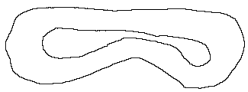
\includegraphics[interpolate=true,width=2.480000in,height=0.920000in]{contents/chapt7/figs/model/unknown_mass_path_1-img3.png}}%
\end{pgfscope}%
\begin{pgfscope}%
\pgfpathrectangle{\pgfqpoint{2.840000in}{0.404960in}}{\pgfqpoint{2.480000in}{0.915692in}}%
\pgfusepath{clip}%
\pgfsetrectcap%
\pgfsetroundjoin%
\pgfsetlinewidth{1.505625pt}%
\definecolor{currentstroke}{rgb}{0.121569,0.466667,0.705882}%
\pgfsetstrokecolor{currentstroke}%
\pgfsetstrokeopacity{0.700000}%
\pgfsetdash{}{0pt}%
\pgfpathmoveto{\pgfqpoint{4.366154in}{1.091729in}}%
\pgfpathlineto{\pgfqpoint{4.289550in}{1.092738in}}%
\pgfpathlineto{\pgfqpoint{4.223126in}{1.095711in}}%
\pgfpathlineto{\pgfqpoint{4.123054in}{1.100447in}}%
\pgfpathlineto{\pgfqpoint{4.063948in}{1.101150in}}%
\pgfpathlineto{\pgfqpoint{3.989144in}{1.099597in}}%
\pgfpathlineto{\pgfqpoint{3.784064in}{1.092808in}}%
\pgfpathlineto{\pgfqpoint{3.601068in}{1.092872in}}%
\pgfpathlineto{\pgfqpoint{3.547733in}{1.089867in}}%
\pgfpathlineto{\pgfqpoint{3.494537in}{1.084748in}}%
\pgfpathlineto{\pgfqpoint{3.441762in}{1.077453in}}%
\pgfpathlineto{\pgfqpoint{3.396773in}{1.069119in}}%
\pgfpathlineto{\pgfqpoint{3.359630in}{1.060279in}}%
\pgfpathlineto{\pgfqpoint{3.323177in}{1.049151in}}%
\pgfpathlineto{\pgfqpoint{3.294694in}{1.038156in}}%
\pgfpathlineto{\pgfqpoint{3.267181in}{1.024909in}}%
\pgfpathlineto{\pgfqpoint{3.247424in}{1.013351in}}%
\pgfpathlineto{\pgfqpoint{3.228635in}{1.000274in}}%
\pgfpathlineto{\pgfqpoint{3.211031in}{0.985668in}}%
\pgfpathlineto{\pgfqpoint{3.194990in}{0.969599in}}%
\pgfpathlineto{\pgfqpoint{3.180773in}{0.952156in}}%
\pgfpathlineto{\pgfqpoint{3.168651in}{0.933442in}}%
\pgfpathlineto{\pgfqpoint{3.158848in}{0.913619in}}%
\pgfpathlineto{\pgfqpoint{3.151557in}{0.892876in}}%
\pgfpathlineto{\pgfqpoint{3.146899in}{0.871514in}}%
\pgfpathlineto{\pgfqpoint{3.144940in}{0.849776in}}%
\pgfpathlineto{\pgfqpoint{3.145610in}{0.827802in}}%
\pgfpathlineto{\pgfqpoint{3.148844in}{0.805855in}}%
\pgfpathlineto{\pgfqpoint{3.154475in}{0.784289in}}%
\pgfpathlineto{\pgfqpoint{3.162381in}{0.763350in}}%
\pgfpathlineto{\pgfqpoint{3.172439in}{0.743272in}}%
\pgfpathlineto{\pgfqpoint{3.184542in}{0.724279in}}%
\pgfpathlineto{\pgfqpoint{3.198533in}{0.706475in}}%
\pgfpathlineto{\pgfqpoint{3.214205in}{0.690010in}}%
\pgfpathlineto{\pgfqpoint{3.231378in}{0.675011in}}%
\pgfpathlineto{\pgfqpoint{3.249851in}{0.661623in}}%
\pgfpathlineto{\pgfqpoint{3.269413in}{0.649950in}}%
\pgfpathlineto{\pgfqpoint{3.289929in}{0.640089in}}%
\pgfpathlineto{\pgfqpoint{3.311270in}{0.632094in}}%
\pgfpathlineto{\pgfqpoint{3.333277in}{0.625869in}}%
\pgfpathlineto{\pgfqpoint{3.363256in}{0.620147in}}%
\pgfpathlineto{\pgfqpoint{3.393572in}{0.617258in}}%
\pgfpathlineto{\pgfqpoint{3.424038in}{0.616962in}}%
\pgfpathlineto{\pgfqpoint{3.454489in}{0.618949in}}%
\pgfpathlineto{\pgfqpoint{3.484746in}{0.623000in}}%
\pgfpathlineto{\pgfqpoint{3.522183in}{0.630524in}}%
\pgfpathlineto{\pgfqpoint{3.559045in}{0.640434in}}%
\pgfpathlineto{\pgfqpoint{3.595191in}{0.652454in}}%
\pgfpathlineto{\pgfqpoint{3.637696in}{0.669296in}}%
\pgfpathlineto{\pgfqpoint{3.715150in}{0.701074in}}%
\pgfpathlineto{\pgfqpoint{3.751003in}{0.713697in}}%
\pgfpathlineto{\pgfqpoint{3.794817in}{0.726374in}}%
\pgfpathlineto{\pgfqpoint{3.839267in}{0.736884in}}%
\pgfpathlineto{\pgfqpoint{3.899258in}{0.748461in}}%
\pgfpathlineto{\pgfqpoint{3.966962in}{0.758991in}}%
\pgfpathlineto{\pgfqpoint{4.027536in}{0.766440in}}%
\pgfpathlineto{\pgfqpoint{4.080711in}{0.770756in}}%
\pgfpathlineto{\pgfqpoint{4.126476in}{0.772255in}}%
\pgfpathlineto{\pgfqpoint{4.172350in}{0.771356in}}%
\pgfpathlineto{\pgfqpoint{4.210420in}{0.768552in}}%
\pgfpathlineto{\pgfqpoint{4.248277in}{0.763728in}}%
\pgfpathlineto{\pgfqpoint{4.285817in}{0.756923in}}%
\pgfpathlineto{\pgfqpoint{4.322961in}{0.748136in}}%
\pgfpathlineto{\pgfqpoint{4.359571in}{0.737456in}}%
\pgfpathlineto{\pgfqpoint{4.439129in}{0.710681in}}%
\pgfpathlineto{\pgfqpoint{4.497398in}{0.692272in}}%
\pgfpathlineto{\pgfqpoint{4.592925in}{0.665731in}}%
\pgfpathlineto{\pgfqpoint{4.695871in}{0.638048in}}%
\pgfpathlineto{\pgfqpoint{4.733232in}{0.630367in}}%
\pgfpathlineto{\pgfqpoint{4.763428in}{0.626059in}}%
\pgfpathlineto{\pgfqpoint{4.793815in}{0.623799in}}%
\pgfpathlineto{\pgfqpoint{4.824335in}{0.623993in}}%
\pgfpathlineto{\pgfqpoint{4.854754in}{0.626907in}}%
\pgfpathlineto{\pgfqpoint{4.877272in}{0.631056in}}%
\pgfpathlineto{\pgfqpoint{4.899350in}{0.636935in}}%
\pgfpathlineto{\pgfqpoint{4.920873in}{0.644619in}}%
\pgfpathlineto{\pgfqpoint{4.941664in}{0.654122in}}%
\pgfpathlineto{\pgfqpoint{4.961257in}{0.665338in}}%
\pgfpathlineto{\pgfqpoint{4.979309in}{0.678146in}}%
\pgfpathlineto{\pgfqpoint{4.995629in}{0.692549in}}%
\pgfpathlineto{\pgfqpoint{5.010012in}{0.708552in}}%
\pgfpathlineto{\pgfqpoint{5.022235in}{0.725938in}}%
\pgfpathlineto{\pgfqpoint{5.032129in}{0.744471in}}%
\pgfpathlineto{\pgfqpoint{5.039658in}{0.763873in}}%
\pgfpathlineto{\pgfqpoint{5.044846in}{0.784001in}}%
\pgfpathlineto{\pgfqpoint{5.047668in}{0.804529in}}%
\pgfpathlineto{\pgfqpoint{5.048203in}{0.825160in}}%
\pgfpathlineto{\pgfqpoint{5.046547in}{0.845661in}}%
\pgfpathlineto{\pgfqpoint{5.042753in}{0.865884in}}%
\pgfpathlineto{\pgfqpoint{5.036941in}{0.885567in}}%
\pgfpathlineto{\pgfqpoint{5.029169in}{0.904583in}}%
\pgfpathlineto{\pgfqpoint{5.019540in}{0.922808in}}%
\pgfpathlineto{\pgfqpoint{5.008150in}{0.940109in}}%
\pgfpathlineto{\pgfqpoint{4.995177in}{0.956301in}}%
\pgfpathlineto{\pgfqpoint{4.980755in}{0.971354in}}%
\pgfpathlineto{\pgfqpoint{4.964938in}{0.985238in}}%
\pgfpathlineto{\pgfqpoint{4.947998in}{0.997787in}}%
\pgfpathlineto{\pgfqpoint{4.923747in}{1.012653in}}%
\pgfpathlineto{\pgfqpoint{4.897870in}{1.025439in}}%
\pgfpathlineto{\pgfqpoint{4.870573in}{1.036360in}}%
\pgfpathlineto{\pgfqpoint{4.842330in}{1.045430in}}%
\pgfpathlineto{\pgfqpoint{4.813386in}{1.052660in}}%
\pgfpathlineto{\pgfqpoint{4.776499in}{1.059358in}}%
\pgfpathlineto{\pgfqpoint{4.649742in}{1.079533in}}%
\pgfpathlineto{\pgfqpoint{4.530747in}{1.103812in}}%
\pgfpathlineto{\pgfqpoint{4.485393in}{1.109683in}}%
\pgfpathlineto{\pgfqpoint{4.371564in}{1.121745in}}%
\pgfpathlineto{\pgfqpoint{4.371564in}{1.121745in}}%
\pgfusepath{stroke}%
\end{pgfscope}%
\begin{pgfscope}%
\pgfpathrectangle{\pgfqpoint{2.840000in}{0.404960in}}{\pgfqpoint{2.480000in}{0.915692in}}%
\pgfusepath{clip}%
\pgfsetrectcap%
\pgfsetroundjoin%
\pgfsetlinewidth{1.505625pt}%
\definecolor{currentstroke}{rgb}{1.000000,0.498039,0.054902}%
\pgfsetstrokecolor{currentstroke}%
\pgfsetstrokeopacity{0.700000}%
\pgfsetdash{}{0pt}%
\pgfpathmoveto{\pgfqpoint{4.366154in}{1.091729in}}%
\pgfpathlineto{\pgfqpoint{4.289484in}{1.092739in}}%
\pgfpathlineto{\pgfqpoint{4.223100in}{1.095705in}}%
\pgfpathlineto{\pgfqpoint{4.123006in}{1.100465in}}%
\pgfpathlineto{\pgfqpoint{4.063858in}{1.101229in}}%
\pgfpathlineto{\pgfqpoint{4.004143in}{1.099723in}}%
\pgfpathlineto{\pgfqpoint{3.928992in}{1.095250in}}%
\pgfpathlineto{\pgfqpoint{3.853190in}{1.090958in}}%
\pgfpathlineto{\pgfqpoint{3.799777in}{1.090201in}}%
\pgfpathlineto{\pgfqpoint{3.731162in}{1.092026in}}%
\pgfpathlineto{\pgfqpoint{3.632101in}{1.094898in}}%
\pgfpathlineto{\pgfqpoint{3.571009in}{1.094173in}}%
\pgfpathlineto{\pgfqpoint{3.517639in}{1.091215in}}%
\pgfpathlineto{\pgfqpoint{3.472088in}{1.086528in}}%
\pgfpathlineto{\pgfqpoint{3.426845in}{1.079784in}}%
\pgfpathlineto{\pgfqpoint{3.389533in}{1.072291in}}%
\pgfpathlineto{\pgfqpoint{3.352734in}{1.062742in}}%
\pgfpathlineto{\pgfqpoint{3.323797in}{1.053316in}}%
\pgfpathlineto{\pgfqpoint{3.295531in}{1.041986in}}%
\pgfpathlineto{\pgfqpoint{3.268201in}{1.028452in}}%
\pgfpathlineto{\pgfqpoint{3.248550in}{1.016684in}}%
\pgfpathlineto{\pgfqpoint{3.229861in}{1.003421in}}%
\pgfpathlineto{\pgfqpoint{3.212360in}{0.988658in}}%
\pgfpathlineto{\pgfqpoint{3.196383in}{0.972523in}}%
\pgfpathlineto{\pgfqpoint{3.182253in}{0.955009in}}%
\pgfpathlineto{\pgfqpoint{3.170231in}{0.936252in}}%
\pgfpathlineto{\pgfqpoint{3.160552in}{0.916337in}}%
\pgfpathlineto{\pgfqpoint{3.153416in}{0.895507in}}%
\pgfpathlineto{\pgfqpoint{3.148994in}{0.874108in}}%
\pgfpathlineto{\pgfqpoint{3.147311in}{0.852447in}}%
\pgfpathlineto{\pgfqpoint{3.148348in}{0.830536in}}%
\pgfpathlineto{\pgfqpoint{3.151986in}{0.808735in}}%
\pgfpathlineto{\pgfqpoint{3.158028in}{0.787290in}}%
\pgfpathlineto{\pgfqpoint{3.166284in}{0.766483in}}%
\pgfpathlineto{\pgfqpoint{3.176589in}{0.746493in}}%
\pgfpathlineto{\pgfqpoint{3.188804in}{0.727549in}}%
\pgfpathlineto{\pgfqpoint{3.202768in}{0.709882in}}%
\pgfpathlineto{\pgfqpoint{3.218322in}{0.693604in}}%
\pgfpathlineto{\pgfqpoint{3.235350in}{0.678881in}}%
\pgfpathlineto{\pgfqpoint{3.253723in}{0.665825in}}%
\pgfpathlineto{\pgfqpoint{3.273346in}{0.654508in}}%
\pgfpathlineto{\pgfqpoint{3.294006in}{0.645004in}}%
\pgfpathlineto{\pgfqpoint{3.315447in}{0.637303in}}%
\pgfpathlineto{\pgfqpoint{3.337490in}{0.631415in}}%
\pgfpathlineto{\pgfqpoint{3.367457in}{0.626049in}}%
\pgfpathlineto{\pgfqpoint{3.397841in}{0.623348in}}%
\pgfpathlineto{\pgfqpoint{3.428367in}{0.623085in}}%
\pgfpathlineto{\pgfqpoint{3.458824in}{0.625018in}}%
\pgfpathlineto{\pgfqpoint{3.489074in}{0.628963in}}%
\pgfpathlineto{\pgfqpoint{3.518966in}{0.634791in}}%
\pgfpathlineto{\pgfqpoint{3.548518in}{0.642448in}}%
\pgfpathlineto{\pgfqpoint{3.584685in}{0.654413in}}%
\pgfpathlineto{\pgfqpoint{3.619870in}{0.668737in}}%
\pgfpathlineto{\pgfqpoint{3.661033in}{0.688363in}}%
\pgfpathlineto{\pgfqpoint{3.722939in}{0.717932in}}%
\pgfpathlineto{\pgfqpoint{3.758323in}{0.732226in}}%
\pgfpathlineto{\pgfqpoint{3.794559in}{0.744201in}}%
\pgfpathlineto{\pgfqpoint{3.831438in}{0.753908in}}%
\pgfpathlineto{\pgfqpoint{3.868814in}{0.761478in}}%
\pgfpathlineto{\pgfqpoint{3.914131in}{0.768265in}}%
\pgfpathlineto{\pgfqpoint{3.967250in}{0.773906in}}%
\pgfpathlineto{\pgfqpoint{4.020538in}{0.777340in}}%
\pgfpathlineto{\pgfqpoint{4.073922in}{0.778668in}}%
\pgfpathlineto{\pgfqpoint{4.119598in}{0.777721in}}%
\pgfpathlineto{\pgfqpoint{4.165175in}{0.774519in}}%
\pgfpathlineto{\pgfqpoint{4.210530in}{0.768802in}}%
\pgfpathlineto{\pgfqpoint{4.262967in}{0.759273in}}%
\pgfpathlineto{\pgfqpoint{4.314750in}{0.747415in}}%
\pgfpathlineto{\pgfqpoint{4.373359in}{0.731322in}}%
\pgfpathlineto{\pgfqpoint{4.504531in}{0.691806in}}%
\pgfpathlineto{\pgfqpoint{4.657927in}{0.645891in}}%
\pgfpathlineto{\pgfqpoint{4.702622in}{0.635442in}}%
\pgfpathlineto{\pgfqpoint{4.740331in}{0.629124in}}%
\pgfpathlineto{\pgfqpoint{4.770741in}{0.626063in}}%
\pgfpathlineto{\pgfqpoint{4.801279in}{0.625158in}}%
\pgfpathlineto{\pgfqpoint{4.831772in}{0.626697in}}%
\pgfpathlineto{\pgfqpoint{4.862038in}{0.630933in}}%
\pgfpathlineto{\pgfqpoint{4.884371in}{0.636052in}}%
\pgfpathlineto{\pgfqpoint{4.906215in}{0.642894in}}%
\pgfpathlineto{\pgfqpoint{4.927397in}{0.651502in}}%
\pgfpathlineto{\pgfqpoint{4.947720in}{0.661863in}}%
\pgfpathlineto{\pgfqpoint{4.966714in}{0.673796in}}%
\pgfpathlineto{\pgfqpoint{4.984125in}{0.687341in}}%
\pgfpathlineto{\pgfqpoint{4.999712in}{0.702444in}}%
\pgfpathlineto{\pgfqpoint{5.013232in}{0.719033in}}%
\pgfpathlineto{\pgfqpoint{5.024488in}{0.736945in}}%
\pgfpathlineto{\pgfqpoint{5.033307in}{0.755894in}}%
\pgfpathlineto{\pgfqpoint{5.039667in}{0.775609in}}%
\pgfpathlineto{\pgfqpoint{5.043541in}{0.795884in}}%
\pgfpathlineto{\pgfqpoint{5.044923in}{0.816436in}}%
\pgfpathlineto{\pgfqpoint{5.043917in}{0.836982in}}%
\pgfpathlineto{\pgfqpoint{5.040660in}{0.857215in}}%
\pgfpathlineto{\pgfqpoint{5.035243in}{0.876924in}}%
\pgfpathlineto{\pgfqpoint{5.027796in}{0.895877in}}%
\pgfpathlineto{\pgfqpoint{5.018293in}{0.914132in}}%
\pgfpathlineto{\pgfqpoint{5.006844in}{0.931743in}}%
\pgfpathlineto{\pgfqpoint{4.993767in}{0.948498in}}%
\pgfpathlineto{\pgfqpoint{4.979190in}{0.964334in}}%
\pgfpathlineto{\pgfqpoint{4.963306in}{0.979123in}}%
\pgfpathlineto{\pgfqpoint{4.940320in}{0.996976in}}%
\pgfpathlineto{\pgfqpoint{4.915416in}{1.012714in}}%
\pgfpathlineto{\pgfqpoint{4.888939in}{1.026258in}}%
\pgfpathlineto{\pgfqpoint{4.861134in}{1.037519in}}%
\pgfpathlineto{\pgfqpoint{4.832468in}{1.046518in}}%
\pgfpathlineto{\pgfqpoint{4.803049in}{1.053282in}}%
\pgfpathlineto{\pgfqpoint{4.773130in}{1.057835in}}%
\pgfpathlineto{\pgfqpoint{4.735385in}{1.061166in}}%
\pgfpathlineto{\pgfqpoint{4.644522in}{1.067959in}}%
\pgfpathlineto{\pgfqpoint{4.606795in}{1.073503in}}%
\pgfpathlineto{\pgfqpoint{4.569325in}{1.080945in}}%
\pgfpathlineto{\pgfqpoint{4.524887in}{1.092130in}}%
\pgfpathlineto{\pgfqpoint{4.466351in}{1.109557in}}%
\pgfpathlineto{\pgfqpoint{4.415026in}{1.124247in}}%
\pgfpathlineto{\pgfqpoint{4.377782in}{1.132376in}}%
\pgfpathlineto{\pgfqpoint{4.370252in}{1.133651in}}%
\pgfpathlineto{\pgfqpoint{4.370252in}{1.133651in}}%
\pgfusepath{stroke}%
\end{pgfscope}%
\begin{pgfscope}%
\definecolor{textcolor}{rgb}{0.000000,0.000000,0.000000}%
\pgfsetstrokecolor{textcolor}%
\pgfsetfillcolor{textcolor}%
\pgftext[x=4.080000in,y=1.403985in,,base]{\color{textcolor}\rmfamily\fontsize{12.000000}{14.400000}\selectfont Steering and velocity controllers}%
\end{pgfscope}%
\begin{pgfscope}%
\pgfsetbuttcap%
\pgfsetmiterjoin%
\definecolor{currentfill}{rgb}{1.000000,1.000000,1.000000}%
\pgfsetfillcolor{currentfill}%
\pgfsetfillopacity{0.800000}%
\pgfsetlinewidth{1.003750pt}%
\definecolor{currentstroke}{rgb}{0.800000,0.800000,0.800000}%
\pgfsetstrokecolor{currentstroke}%
\pgfsetstrokeopacity{0.800000}%
\pgfsetdash{}{0pt}%
\pgfpathmoveto{\pgfqpoint{0.864416in}{0.083333in}}%
\pgfpathlineto{\pgfqpoint{4.635584in}{0.083333in}}%
\pgfpathquadraticcurveto{\pgfqpoint{4.668917in}{0.083333in}}{\pgfqpoint{4.668917in}{0.116667in}}%
\pgfpathlineto{\pgfqpoint{4.668917in}{0.333000in}}%
\pgfpathquadraticcurveto{\pgfqpoint{4.668917in}{0.366333in}}{\pgfqpoint{4.635584in}{0.366333in}}%
\pgfpathlineto{\pgfqpoint{0.864416in}{0.366333in}}%
\pgfpathquadraticcurveto{\pgfqpoint{0.831083in}{0.366333in}}{\pgfqpoint{0.831083in}{0.333000in}}%
\pgfpathlineto{\pgfqpoint{0.831083in}{0.116667in}}%
\pgfpathquadraticcurveto{\pgfqpoint{0.831083in}{0.083333in}}{\pgfqpoint{0.864416in}{0.083333in}}%
\pgfpathlineto{\pgfqpoint{0.864416in}{0.083333in}}%
\pgfpathclose%
\pgfusepath{stroke,fill}%
\end{pgfscope}%
\begin{pgfscope}%
\pgfsetrectcap%
\pgfsetroundjoin%
\pgfsetlinewidth{1.505625pt}%
\definecolor{currentstroke}{rgb}{0.121569,0.466667,0.705882}%
\pgfsetstrokecolor{currentstroke}%
\pgfsetstrokeopacity{0.700000}%
\pgfsetdash{}{0pt}%
\pgfpathmoveto{\pgfqpoint{0.897750in}{0.240667in}}%
\pgfpathlineto{\pgfqpoint{1.064416in}{0.240667in}}%
\pgfpathlineto{\pgfqpoint{1.231083in}{0.240667in}}%
\pgfusepath{stroke}%
\end{pgfscope}%
\begin{pgfscope}%
\definecolor{textcolor}{rgb}{0.000000,0.000000,0.000000}%
\pgfsetstrokecolor{textcolor}%
\pgfsetfillcolor{textcolor}%
\pgftext[x=1.364416in,y=0.182333in,left,base]{\color{textcolor}\rmfamily\fontsize{12.000000}{14.400000}\selectfont No mass}%
\end{pgfscope}%
\begin{pgfscope}%
\pgfsetrectcap%
\pgfsetroundjoin%
\pgfsetlinewidth{1.505625pt}%
\definecolor{currentstroke}{rgb}{1.000000,0.498039,0.054902}%
\pgfsetstrokecolor{currentstroke}%
\pgfsetstrokeopacity{0.700000}%
\pgfsetdash{}{0pt}%
\pgfpathmoveto{\pgfqpoint{2.302417in}{0.240667in}}%
\pgfpathlineto{\pgfqpoint{2.469083in}{0.240667in}}%
\pgfpathlineto{\pgfqpoint{2.635750in}{0.240667in}}%
\pgfusepath{stroke}%
\end{pgfscope}%
\begin{pgfscope}%
\definecolor{textcolor}{rgb}{0.000000,0.000000,0.000000}%
\pgfsetstrokecolor{textcolor}%
\pgfsetfillcolor{textcolor}%
\pgftext[x=2.769083in,y=0.182333in,left,base]{\color{textcolor}\rmfamily\fontsize{12.000000}{14.400000}\selectfont Mass placed on front axle}%
\end{pgfscope}%
\end{pgfpicture}%
\makeatother%
\endgroup%

%     \caption[Paths taken by agents with and without an accounted for mass placed above the front axle]{Paths taken by agents with and without an unaccounted for mass placed above the front axle.}
%     \label{fig:unknown_mass_path}
% \end{figure}

Although Figure \ref{fig:unknown_mass} is a good indicator of the performance of each agent, we would also like to characterise the behaviour of the agents under model-mismatch conditions.
We therefore present the trajectories taken by an end-to-end agent, as well as a partial end-to-end agent with steering and velocity control, under conditions with and without model-mismatch over one lap in Figure \ref{fig:unknown_mass_trajs_2}.

The trajectory of the end-to-end agent is shown on the left of this figure. 
We see that the trajectories by the agent with and without model-mismatch are similar on the first straight section of the track, as well as around the first corner.
However, after the first corner, the end-to-end agent experiences slaloming on both laps.
The slaloming is characterised by fast and large oscillations in slip angle, as well as the selection of extreme steering angles.
Without model-mismatch, the end-to-end agent recovers from slaloming before the second corner.
However, in the presence of model-mismatching, the end-to-end agent is unable to recover from slaloming.
In fact, the oscillations in slip angle and steering angle grow larger until the end of the lap.

From multiple runs, we observed that end-to-end agents typically slalom after performing sharp braking manoeuvres.
End-to-end agents are slow to recover from slaloming under conditions with no model-mismatch.
However, in the presence of model mismatch, end-to-end agents are unable to recover from slaloming, and the vehicle continues to swerve for a long time.
Thus, the effect of model-mismatches are not felt across the entire operating domain of the agent, but are most catastrophic when the agent leaves its normal operating domain by slipping.

The trajectory by the partial end-to-end agent with a steering and a velocity controller is shown on the right side of Figure \ref{fig:unknown_mass_trajs_2}.
We see that the partial end-to-end agent executes near identical trajectories regardless of the presence of model-mismatch.
Decoupling path planning and control is therefore beneficial for scenarios with and without model-mismatches.
The simple feedback steering control provides stability and robustness to model-mismatches.
Furthermore, restricting the path inadvertently smooths the steering controls, and prevents the vehicle from selecting extreme steering angles.
We also see that the addition of the velocity controller smooths the velocity profile.
Selecting smoother control actions makes slipping less likely.


\begin{figure}[htb!]
    \centering
    %% Creator: Matplotlib, PGF backend
%%
%% To include the figure in your LaTeX document, write
%%   \input{<filename>.pgf}
%%
%% Make sure the required packages are loaded in your preamble
%%   \usepackage{pgf}
%%
%% Also ensure that all the required font packages are loaded; for instance,
%% the lmodern package is sometimes necessary when using math font.
%%   \usepackage{lmodern}
%%
%% Figures using additional raster images can only be included by \input if
%% they are in the same directory as the main LaTeX file. For loading figures
%% from other directories you can use the `import` package
%%   \usepackage{import}
%%
%% and then include the figures with
%%   \import{<path to file>}{<filename>.pgf}
%%
%% Matplotlib used the following preamble
%%   \usepackage{fontspec}
%%   \setmainfont{DejaVuSerif.ttf}[Path=\detokenize{/home/andrew/anaconda3/envs/auto_car_env/lib/python3.9/site-packages/matplotlib/mpl-data/fonts/ttf/}]
%%   \setsansfont{DejaVuSans.ttf}[Path=\detokenize{/home/andrew/anaconda3/envs/auto_car_env/lib/python3.9/site-packages/matplotlib/mpl-data/fonts/ttf/}]
%%   \setmonofont{DejaVuSansMono.ttf}[Path=\detokenize{/home/andrew/anaconda3/envs/auto_car_env/lib/python3.9/site-packages/matplotlib/mpl-data/fonts/ttf/}]
%%
\begingroup%
\makeatletter%
\begin{pgfpicture}%
\pgfpathrectangle{\pgfpointorigin}{\pgfqpoint{5.500000in}{5.000000in}}%
\pgfusepath{use as bounding box, clip}%
\begin{pgfscope}%
\pgfsetbuttcap%
\pgfsetmiterjoin%
\definecolor{currentfill}{rgb}{1.000000,1.000000,1.000000}%
\pgfsetfillcolor{currentfill}%
\pgfsetlinewidth{0.000000pt}%
\definecolor{currentstroke}{rgb}{1.000000,1.000000,1.000000}%
\pgfsetstrokecolor{currentstroke}%
\pgfsetdash{}{0pt}%
\pgfpathmoveto{\pgfqpoint{0.000000in}{0.000000in}}%
\pgfpathlineto{\pgfqpoint{5.500000in}{0.000000in}}%
\pgfpathlineto{\pgfqpoint{5.500000in}{5.000000in}}%
\pgfpathlineto{\pgfqpoint{0.000000in}{5.000000in}}%
\pgfpathlineto{\pgfqpoint{0.000000in}{0.000000in}}%
\pgfpathclose%
\pgfusepath{fill}%
\end{pgfscope}%
\begin{pgfscope}%
\pgfpathrectangle{\pgfqpoint{1.054417in}{3.950574in}}{\pgfqpoint{1.996630in}{0.737217in}}%
\pgfusepath{clip}%
\pgfsys@transformshift{1.054417in}{3.950574in}%
\pgftext[left,bottom]{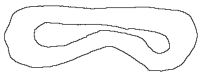
\includegraphics[interpolate=true,width=2.000000in,height=0.740000in]{contents/chapt7/figs/model/unknown_mass_trajs_3-img0.png}}%
\end{pgfscope}%
\begin{pgfscope}%
\pgfpathrectangle{\pgfqpoint{1.054417in}{3.950574in}}{\pgfqpoint{1.996630in}{0.737217in}}%
\pgfusepath{clip}%
\pgfsetbuttcap%
\pgfsetroundjoin%
\pgfsetlinewidth{1.505625pt}%
\definecolor{currentstroke}{rgb}{1.000000,0.000000,0.000000}%
\pgfsetstrokecolor{currentstroke}%
\pgfsetdash{{1.500000pt}{2.475000pt}}{0.000000pt}%
\pgfpathmoveto{\pgfqpoint{2.278748in}{4.384629in}}%
\pgfpathlineto{\pgfqpoint{2.278748in}{4.630368in}}%
\pgfusepath{stroke}%
\end{pgfscope}%
\begin{pgfscope}%
\pgfpathrectangle{\pgfqpoint{1.054417in}{3.950574in}}{\pgfqpoint{1.996630in}{0.737217in}}%
\pgfusepath{clip}%
\pgfsetrectcap%
\pgfsetroundjoin%
\pgfsetlinewidth{1.505625pt}%
\definecolor{currentstroke}{rgb}{0.121569,0.466667,0.705882}%
\pgfsetstrokecolor{currentstroke}%
\pgfsetstrokeopacity{0.700000}%
\pgfsetdash{}{0pt}%
\pgfpathmoveto{\pgfqpoint{2.283112in}{4.503487in}}%
\pgfpathlineto{\pgfqpoint{2.245241in}{4.504362in}}%
\pgfpathlineto{\pgfqpoint{2.217502in}{4.507128in}}%
\pgfpathlineto{\pgfqpoint{2.188712in}{4.512170in}}%
\pgfpathlineto{\pgfqpoint{2.112549in}{4.526987in}}%
\pgfpathlineto{\pgfqpoint{2.068930in}{4.533041in}}%
\pgfpathlineto{\pgfqpoint{2.022634in}{4.537055in}}%
\pgfpathlineto{\pgfqpoint{1.980029in}{4.538555in}}%
\pgfpathlineto{\pgfqpoint{1.825671in}{4.541670in}}%
\pgfpathlineto{\pgfqpoint{1.628242in}{4.550546in}}%
\pgfpathlineto{\pgfqpoint{1.572661in}{4.550689in}}%
\pgfpathlineto{\pgfqpoint{1.535656in}{4.548806in}}%
\pgfpathlineto{\pgfqpoint{1.498843in}{4.544620in}}%
\pgfpathlineto{\pgfqpoint{1.468492in}{4.538952in}}%
\pgfpathlineto{\pgfqpoint{1.438654in}{4.531023in}}%
\pgfpathlineto{\pgfqpoint{1.409555in}{4.520710in}}%
\pgfpathlineto{\pgfqpoint{1.381445in}{4.507947in}}%
\pgfpathlineto{\pgfqpoint{1.359859in}{4.495942in}}%
\pgfpathlineto{\pgfqpoint{1.339480in}{4.481996in}}%
\pgfpathlineto{\pgfqpoint{1.325323in}{4.470052in}}%
\pgfpathlineto{\pgfqpoint{1.312377in}{4.456805in}}%
\pgfpathlineto{\pgfqpoint{1.300919in}{4.442255in}}%
\pgfpathlineto{\pgfqpoint{1.291215in}{4.426482in}}%
\pgfpathlineto{\pgfqpoint{1.283509in}{4.409643in}}%
\pgfpathlineto{\pgfqpoint{1.277949in}{4.391980in}}%
\pgfpathlineto{\pgfqpoint{1.274665in}{4.373755in}}%
\pgfpathlineto{\pgfqpoint{1.273740in}{4.355261in}}%
\pgfpathlineto{\pgfqpoint{1.275177in}{4.336799in}}%
\pgfpathlineto{\pgfqpoint{1.278960in}{4.318672in}}%
\pgfpathlineto{\pgfqpoint{1.285011in}{4.301171in}}%
\pgfpathlineto{\pgfqpoint{1.293118in}{4.284520in}}%
\pgfpathlineto{\pgfqpoint{1.302949in}{4.268822in}}%
\pgfpathlineto{\pgfqpoint{1.314252in}{4.254148in}}%
\pgfpathlineto{\pgfqpoint{1.331244in}{4.236231in}}%
\pgfpathlineto{\pgfqpoint{1.349995in}{4.220159in}}%
\pgfpathlineto{\pgfqpoint{1.370120in}{4.205842in}}%
\pgfpathlineto{\pgfqpoint{1.396555in}{4.189890in}}%
\pgfpathlineto{\pgfqpoint{1.429461in}{4.172858in}}%
\pgfpathlineto{\pgfqpoint{1.474396in}{4.152437in}}%
\pgfpathlineto{\pgfqpoint{1.512950in}{4.137103in}}%
\pgfpathlineto{\pgfqpoint{1.539819in}{4.128703in}}%
\pgfpathlineto{\pgfqpoint{1.566118in}{4.123014in}}%
\pgfpathlineto{\pgfqpoint{1.586910in}{4.120758in}}%
\pgfpathlineto{\pgfqpoint{1.608431in}{4.120762in}}%
\pgfpathlineto{\pgfqpoint{1.630549in}{4.122895in}}%
\pgfpathlineto{\pgfqpoint{1.653090in}{4.127051in}}%
\pgfpathlineto{\pgfqpoint{1.675890in}{4.133222in}}%
\pgfpathlineto{\pgfqpoint{1.698856in}{4.141467in}}%
\pgfpathlineto{\pgfqpoint{1.726953in}{4.154139in}}%
\pgfpathlineto{\pgfqpoint{1.759504in}{4.171703in}}%
\pgfpathlineto{\pgfqpoint{1.796119in}{4.194544in}}%
\pgfpathlineto{\pgfqpoint{1.853191in}{4.231166in}}%
\pgfpathlineto{\pgfqpoint{1.880497in}{4.245456in}}%
\pgfpathlineto{\pgfqpoint{1.903287in}{4.254863in}}%
\pgfpathlineto{\pgfqpoint{1.926868in}{4.262063in}}%
\pgfpathlineto{\pgfqpoint{1.950982in}{4.267208in}}%
\pgfpathlineto{\pgfqpoint{1.981548in}{4.271159in}}%
\pgfpathlineto{\pgfqpoint{2.012326in}{4.272846in}}%
\pgfpathlineto{\pgfqpoint{2.055481in}{4.272565in}}%
\pgfpathlineto{\pgfqpoint{2.117131in}{4.272002in}}%
\pgfpathlineto{\pgfqpoint{2.154052in}{4.274187in}}%
\pgfpathlineto{\pgfqpoint{2.190744in}{4.278885in}}%
\pgfpathlineto{\pgfqpoint{2.251831in}{4.287153in}}%
\pgfpathlineto{\pgfqpoint{2.276404in}{4.288307in}}%
\pgfpathlineto{\pgfqpoint{2.300234in}{4.287362in}}%
\pgfpathlineto{\pgfqpoint{2.322888in}{4.283856in}}%
\pgfpathlineto{\pgfqpoint{2.338858in}{4.279357in}}%
\pgfpathlineto{\pgfqpoint{2.353709in}{4.273209in}}%
\pgfpathlineto{\pgfqpoint{2.367215in}{4.265492in}}%
\pgfpathlineto{\pgfqpoint{2.379214in}{4.256278in}}%
\pgfpathlineto{\pgfqpoint{2.390010in}{4.245357in}}%
\pgfpathlineto{\pgfqpoint{2.402975in}{4.228872in}}%
\pgfpathlineto{\pgfqpoint{2.427194in}{4.192553in}}%
\pgfpathlineto{\pgfqpoint{2.449931in}{4.159760in}}%
\pgfpathlineto{\pgfqpoint{2.468202in}{4.137316in}}%
\pgfpathlineto{\pgfqpoint{2.484428in}{4.120514in}}%
\pgfpathlineto{\pgfqpoint{2.502199in}{4.105079in}}%
\pgfpathlineto{\pgfqpoint{2.521508in}{4.091306in}}%
\pgfpathlineto{\pgfqpoint{2.542695in}{4.079217in}}%
\pgfpathlineto{\pgfqpoint{2.565182in}{4.069252in}}%
\pgfpathlineto{\pgfqpoint{2.588596in}{4.061724in}}%
\pgfpathlineto{\pgfqpoint{2.612717in}{4.056936in}}%
\pgfpathlineto{\pgfqpoint{2.631093in}{4.055299in}}%
\pgfpathlineto{\pgfqpoint{2.649542in}{4.055410in}}%
\pgfpathlineto{\pgfqpoint{2.667898in}{4.057247in}}%
\pgfpathlineto{\pgfqpoint{2.686001in}{4.060800in}}%
\pgfpathlineto{\pgfqpoint{2.703690in}{4.066041in}}%
\pgfpathlineto{\pgfqpoint{2.720817in}{4.072899in}}%
\pgfpathlineto{\pgfqpoint{2.737237in}{4.081310in}}%
\pgfpathlineto{\pgfqpoint{2.752821in}{4.091183in}}%
\pgfpathlineto{\pgfqpoint{2.767417in}{4.102466in}}%
\pgfpathlineto{\pgfqpoint{2.780870in}{4.115090in}}%
\pgfpathlineto{\pgfqpoint{2.793054in}{4.128942in}}%
\pgfpathlineto{\pgfqpoint{2.803830in}{4.143916in}}%
\pgfpathlineto{\pgfqpoint{2.813081in}{4.159876in}}%
\pgfpathlineto{\pgfqpoint{2.820692in}{4.176681in}}%
\pgfpathlineto{\pgfqpoint{2.826581in}{4.194163in}}%
\pgfpathlineto{\pgfqpoint{2.830744in}{4.212135in}}%
\pgfpathlineto{\pgfqpoint{2.833146in}{4.230427in}}%
\pgfpathlineto{\pgfqpoint{2.833793in}{4.248864in}}%
\pgfpathlineto{\pgfqpoint{2.832695in}{4.267280in}}%
\pgfpathlineto{\pgfqpoint{2.829896in}{4.285515in}}%
\pgfpathlineto{\pgfqpoint{2.825426in}{4.303414in}}%
\pgfpathlineto{\pgfqpoint{2.816983in}{4.326512in}}%
\pgfpathlineto{\pgfqpoint{2.806027in}{4.348531in}}%
\pgfpathlineto{\pgfqpoint{2.792793in}{4.369263in}}%
\pgfpathlineto{\pgfqpoint{2.777535in}{4.388555in}}%
\pgfpathlineto{\pgfqpoint{2.760496in}{4.406295in}}%
\pgfpathlineto{\pgfqpoint{2.741898in}{4.422395in}}%
\pgfpathlineto{\pgfqpoint{2.722059in}{4.436942in}}%
\pgfpathlineto{\pgfqpoint{2.701182in}{4.449956in}}%
\pgfpathlineto{\pgfqpoint{2.673907in}{4.464153in}}%
\pgfpathlineto{\pgfqpoint{2.645591in}{4.476144in}}%
\pgfpathlineto{\pgfqpoint{2.610637in}{4.487975in}}%
\pgfpathlineto{\pgfqpoint{2.574992in}{4.497532in}}%
\pgfpathlineto{\pgfqpoint{2.532847in}{4.506341in}}%
\pgfpathlineto{\pgfqpoint{2.484249in}{4.514070in}}%
\pgfpathlineto{\pgfqpoint{2.423181in}{4.521452in}}%
\pgfpathlineto{\pgfqpoint{2.361913in}{4.526923in}}%
\pgfpathlineto{\pgfqpoint{2.306621in}{4.529664in}}%
\pgfpathlineto{\pgfqpoint{2.294321in}{4.529931in}}%
\pgfpathlineto{\pgfqpoint{2.294321in}{4.529931in}}%
\pgfusepath{stroke}%
\end{pgfscope}%
\begin{pgfscope}%
\pgfpathrectangle{\pgfqpoint{1.054417in}{3.950574in}}{\pgfqpoint{1.996630in}{0.737217in}}%
\pgfusepath{clip}%
\pgfsetrectcap%
\pgfsetroundjoin%
\pgfsetlinewidth{1.505625pt}%
\definecolor{currentstroke}{rgb}{1.000000,0.498039,0.054902}%
\pgfsetstrokecolor{currentstroke}%
\pgfsetstrokeopacity{0.700000}%
\pgfsetdash{}{0pt}%
\pgfpathmoveto{\pgfqpoint{2.283112in}{4.503487in}}%
\pgfpathlineto{\pgfqpoint{2.241150in}{4.504500in}}%
\pgfpathlineto{\pgfqpoint{2.208781in}{4.507544in}}%
\pgfpathlineto{\pgfqpoint{2.169518in}{4.513820in}}%
\pgfpathlineto{\pgfqpoint{2.092066in}{4.526169in}}%
\pgfpathlineto{\pgfqpoint{2.045712in}{4.531466in}}%
\pgfpathlineto{\pgfqpoint{2.003043in}{4.534353in}}%
\pgfpathlineto{\pgfqpoint{1.953725in}{4.535193in}}%
\pgfpathlineto{\pgfqpoint{1.805755in}{4.535986in}}%
\pgfpathlineto{\pgfqpoint{1.738040in}{4.539845in}}%
\pgfpathlineto{\pgfqpoint{1.565800in}{4.551515in}}%
\pgfpathlineto{\pgfqpoint{1.528811in}{4.551080in}}%
\pgfpathlineto{\pgfqpoint{1.498087in}{4.548593in}}%
\pgfpathlineto{\pgfqpoint{1.467649in}{4.543740in}}%
\pgfpathlineto{\pgfqpoint{1.437735in}{4.536315in}}%
\pgfpathlineto{\pgfqpoint{1.408610in}{4.526231in}}%
\pgfpathlineto{\pgfqpoint{1.386054in}{4.516267in}}%
\pgfpathlineto{\pgfqpoint{1.364299in}{4.504655in}}%
\pgfpathlineto{\pgfqpoint{1.343612in}{4.491241in}}%
\pgfpathlineto{\pgfqpoint{1.324512in}{4.475657in}}%
\pgfpathlineto{\pgfqpoint{1.311557in}{4.462462in}}%
\pgfpathlineto{\pgfqpoint{1.300043in}{4.447994in}}%
\pgfpathlineto{\pgfqpoint{1.290258in}{4.432307in}}%
\pgfpathlineto{\pgfqpoint{1.282463in}{4.415542in}}%
\pgfpathlineto{\pgfqpoint{1.276790in}{4.397946in}}%
\pgfpathlineto{\pgfqpoint{1.273349in}{4.379781in}}%
\pgfpathlineto{\pgfqpoint{1.272230in}{4.361328in}}%
\pgfpathlineto{\pgfqpoint{1.273427in}{4.342878in}}%
\pgfpathlineto{\pgfqpoint{1.276906in}{4.324721in}}%
\pgfpathlineto{\pgfqpoint{1.282578in}{4.307124in}}%
\pgfpathlineto{\pgfqpoint{1.290327in}{4.290337in}}%
\pgfpathlineto{\pgfqpoint{1.299854in}{4.274488in}}%
\pgfpathlineto{\pgfqpoint{1.314789in}{4.254876in}}%
\pgfpathlineto{\pgfqpoint{1.331844in}{4.237072in}}%
\pgfpathlineto{\pgfqpoint{1.350558in}{4.221018in}}%
\pgfpathlineto{\pgfqpoint{1.370530in}{4.206626in}}%
\pgfpathlineto{\pgfqpoint{1.391410in}{4.193979in}}%
\pgfpathlineto{\pgfqpoint{1.413010in}{4.183085in}}%
\pgfpathlineto{\pgfqpoint{1.435195in}{4.174005in}}%
\pgfpathlineto{\pgfqpoint{1.457829in}{4.166809in}}%
\pgfpathlineto{\pgfqpoint{1.480747in}{4.161531in}}%
\pgfpathlineto{\pgfqpoint{1.509432in}{4.157344in}}%
\pgfpathlineto{\pgfqpoint{1.537916in}{4.155686in}}%
\pgfpathlineto{\pgfqpoint{1.565985in}{4.156275in}}%
\pgfpathlineto{\pgfqpoint{1.593658in}{4.158859in}}%
\pgfpathlineto{\pgfqpoint{1.627715in}{4.164179in}}%
\pgfpathlineto{\pgfqpoint{1.674912in}{4.174020in}}%
\pgfpathlineto{\pgfqpoint{1.722750in}{4.186090in}}%
\pgfpathlineto{\pgfqpoint{1.764041in}{4.198685in}}%
\pgfpathlineto{\pgfqpoint{1.798806in}{4.211354in}}%
\pgfpathlineto{\pgfqpoint{1.838439in}{4.228462in}}%
\pgfpathlineto{\pgfqpoint{1.939612in}{4.274134in}}%
\pgfpathlineto{\pgfqpoint{1.968598in}{4.284640in}}%
\pgfpathlineto{\pgfqpoint{1.992358in}{4.291261in}}%
\pgfpathlineto{\pgfqpoint{2.016577in}{4.295919in}}%
\pgfpathlineto{\pgfqpoint{2.041128in}{4.298240in}}%
\pgfpathlineto{\pgfqpoint{2.065785in}{4.297949in}}%
\pgfpathlineto{\pgfqpoint{2.090298in}{4.295228in}}%
\pgfpathlineto{\pgfqpoint{2.120551in}{4.289283in}}%
\pgfpathlineto{\pgfqpoint{2.240850in}{4.262225in}}%
\pgfpathlineto{\pgfqpoint{2.277580in}{4.257764in}}%
\pgfpathlineto{\pgfqpoint{2.320064in}{4.255298in}}%
\pgfpathlineto{\pgfqpoint{2.377354in}{4.252093in}}%
\pgfpathlineto{\pgfqpoint{2.404259in}{4.248420in}}%
\pgfpathlineto{\pgfqpoint{2.424920in}{4.243650in}}%
\pgfpathlineto{\pgfqpoint{2.444714in}{4.236948in}}%
\pgfpathlineto{\pgfqpoint{2.463393in}{4.228284in}}%
\pgfpathlineto{\pgfqpoint{2.480728in}{4.217749in}}%
\pgfpathlineto{\pgfqpoint{2.496520in}{4.205511in}}%
\pgfpathlineto{\pgfqpoint{2.511246in}{4.191338in}}%
\pgfpathlineto{\pgfqpoint{2.536469in}{4.162958in}}%
\pgfpathlineto{\pgfqpoint{2.567829in}{4.128203in}}%
\pgfpathlineto{\pgfqpoint{2.589774in}{4.106953in}}%
\pgfpathlineto{\pgfqpoint{2.608868in}{4.091673in}}%
\pgfpathlineto{\pgfqpoint{2.629579in}{4.078642in}}%
\pgfpathlineto{\pgfqpoint{2.646158in}{4.070738in}}%
\pgfpathlineto{\pgfqpoint{2.663529in}{4.064741in}}%
\pgfpathlineto{\pgfqpoint{2.681566in}{4.060892in}}%
\pgfpathlineto{\pgfqpoint{2.700067in}{4.059453in}}%
\pgfpathlineto{\pgfqpoint{2.718590in}{4.060580in}}%
\pgfpathlineto{\pgfqpoint{2.736763in}{4.064332in}}%
\pgfpathlineto{\pgfqpoint{2.754173in}{4.070748in}}%
\pgfpathlineto{\pgfqpoint{2.770388in}{4.079765in}}%
\pgfpathlineto{\pgfqpoint{2.784966in}{4.091241in}}%
\pgfpathlineto{\pgfqpoint{2.797499in}{4.104919in}}%
\pgfpathlineto{\pgfqpoint{2.807733in}{4.120396in}}%
\pgfpathlineto{\pgfqpoint{2.815620in}{4.137195in}}%
\pgfpathlineto{\pgfqpoint{2.821205in}{4.154893in}}%
\pgfpathlineto{\pgfqpoint{2.824509in}{4.173157in}}%
\pgfpathlineto{\pgfqpoint{2.825666in}{4.191683in}}%
\pgfpathlineto{\pgfqpoint{2.824821in}{4.210227in}}%
\pgfpathlineto{\pgfqpoint{2.820993in}{4.234678in}}%
\pgfpathlineto{\pgfqpoint{2.814870in}{4.258664in}}%
\pgfpathlineto{\pgfqpoint{2.803183in}{4.293912in}}%
\pgfpathlineto{\pgfqpoint{2.768350in}{4.386624in}}%
\pgfpathlineto{\pgfqpoint{2.755615in}{4.414824in}}%
\pgfpathlineto{\pgfqpoint{2.743233in}{4.436254in}}%
\pgfpathlineto{\pgfqpoint{2.732308in}{4.451263in}}%
\pgfpathlineto{\pgfqpoint{2.719823in}{4.464997in}}%
\pgfpathlineto{\pgfqpoint{2.705744in}{4.477090in}}%
\pgfpathlineto{\pgfqpoint{2.690182in}{4.487200in}}%
\pgfpathlineto{\pgfqpoint{2.673348in}{4.495006in}}%
\pgfpathlineto{\pgfqpoint{2.655553in}{4.500264in}}%
\pgfpathlineto{\pgfqpoint{2.637171in}{4.502787in}}%
\pgfpathlineto{\pgfqpoint{2.618616in}{4.502545in}}%
\pgfpathlineto{\pgfqpoint{2.600269in}{4.499751in}}%
\pgfpathlineto{\pgfqpoint{2.582405in}{4.494710in}}%
\pgfpathlineto{\pgfqpoint{2.565167in}{4.487819in}}%
\pgfpathlineto{\pgfqpoint{2.543125in}{4.476554in}}%
\pgfpathlineto{\pgfqpoint{2.481955in}{4.442366in}}%
\pgfpathlineto{\pgfqpoint{2.463342in}{4.435367in}}%
\pgfpathlineto{\pgfqpoint{2.449971in}{4.432392in}}%
\pgfpathlineto{\pgfqpoint{2.437342in}{4.431647in}}%
\pgfpathlineto{\pgfqpoint{2.425682in}{4.433420in}}%
\pgfpathlineto{\pgfqpoint{2.414342in}{4.438360in}}%
\pgfpathlineto{\pgfqpoint{2.399569in}{4.448106in}}%
\pgfpathlineto{\pgfqpoint{2.376964in}{4.466452in}}%
\pgfpathlineto{\pgfqpoint{2.356578in}{4.483545in}}%
\pgfpathlineto{\pgfqpoint{2.356578in}{4.483545in}}%
\pgfusepath{stroke}%
\end{pgfscope}%
\begin{pgfscope}%
\pgfsetbuttcap%
\pgfsetmiterjoin%
\definecolor{currentfill}{rgb}{1.000000,1.000000,1.000000}%
\pgfsetfillcolor{currentfill}%
\pgfsetlinewidth{1.003750pt}%
\definecolor{currentstroke}{rgb}{0.000000,0.000000,0.000000}%
\pgfsetstrokecolor{currentstroke}%
\pgfsetdash{}{0pt}%
\pgfpathmoveto{\pgfqpoint{1.518815in}{4.503820in}}%
\pgfpathlineto{\pgfqpoint{1.775964in}{4.503820in}}%
\pgfpathquadraticcurveto{\pgfqpoint{1.787534in}{4.503820in}}{\pgfqpoint{1.787534in}{4.515389in}}%
\pgfpathlineto{\pgfqpoint{1.787534in}{4.627355in}}%
\pgfpathquadraticcurveto{\pgfqpoint{1.787534in}{4.638924in}}{\pgfqpoint{1.775964in}{4.638924in}}%
\pgfpathlineto{\pgfqpoint{1.518815in}{4.638924in}}%
\pgfpathquadraticcurveto{\pgfqpoint{1.507246in}{4.638924in}}{\pgfqpoint{1.507246in}{4.627355in}}%
\pgfpathlineto{\pgfqpoint{1.507246in}{4.515389in}}%
\pgfpathquadraticcurveto{\pgfqpoint{1.507246in}{4.503820in}}{\pgfqpoint{1.518815in}{4.503820in}}%
\pgfpathlineto{\pgfqpoint{1.518815in}{4.503820in}}%
\pgfpathclose%
\pgfusepath{stroke,fill}%
\end{pgfscope}%
\begin{pgfscope}%
\definecolor{textcolor}{rgb}{0.000000,0.000000,0.000000}%
\pgfsetstrokecolor{textcolor}%
\pgfsetfillcolor{textcolor}%
\pgftext[x=1.518815in,y=4.539454in,left,base]{\color{textcolor}\rmfamily\fontsize{8.330000}{9.996000}\selectfont 20\%}%
\end{pgfscope}%
\begin{pgfscope}%
\pgfsetbuttcap%
\pgfsetmiterjoin%
\definecolor{currentfill}{rgb}{1.000000,1.000000,1.000000}%
\pgfsetfillcolor{currentfill}%
\pgfsetlinewidth{1.003750pt}%
\definecolor{currentstroke}{rgb}{0.000000,0.000000,0.000000}%
\pgfsetstrokecolor{currentstroke}%
\pgfsetdash{}{0pt}%
\pgfpathmoveto{\pgfqpoint{1.516473in}{4.087225in}}%
\pgfpathlineto{\pgfqpoint{1.773622in}{4.087225in}}%
\pgfpathquadraticcurveto{\pgfqpoint{1.785192in}{4.087225in}}{\pgfqpoint{1.785192in}{4.098794in}}%
\pgfpathlineto{\pgfqpoint{1.785192in}{4.210760in}}%
\pgfpathquadraticcurveto{\pgfqpoint{1.785192in}{4.222329in}}{\pgfqpoint{1.773622in}{4.222329in}}%
\pgfpathlineto{\pgfqpoint{1.516473in}{4.222329in}}%
\pgfpathquadraticcurveto{\pgfqpoint{1.504904in}{4.222329in}}{\pgfqpoint{1.504904in}{4.210760in}}%
\pgfpathlineto{\pgfqpoint{1.504904in}{4.098794in}}%
\pgfpathquadraticcurveto{\pgfqpoint{1.504904in}{4.087225in}}{\pgfqpoint{1.516473in}{4.087225in}}%
\pgfpathlineto{\pgfqpoint{1.516473in}{4.087225in}}%
\pgfpathclose%
\pgfusepath{stroke,fill}%
\end{pgfscope}%
\begin{pgfscope}%
\definecolor{textcolor}{rgb}{0.000000,0.000000,0.000000}%
\pgfsetstrokecolor{textcolor}%
\pgfsetfillcolor{textcolor}%
\pgftext[x=1.516473in,y=4.122859in,left,base]{\color{textcolor}\rmfamily\fontsize{8.330000}{9.996000}\selectfont 40\%}%
\end{pgfscope}%
\begin{pgfscope}%
\pgfsetbuttcap%
\pgfsetmiterjoin%
\definecolor{currentfill}{rgb}{1.000000,1.000000,1.000000}%
\pgfsetfillcolor{currentfill}%
\pgfsetlinewidth{1.003750pt}%
\definecolor{currentstroke}{rgb}{0.000000,0.000000,0.000000}%
\pgfsetstrokecolor{currentstroke}%
\pgfsetdash{}{0pt}%
\pgfpathmoveto{\pgfqpoint{2.243577in}{4.248009in}}%
\pgfpathlineto{\pgfqpoint{2.500726in}{4.248009in}}%
\pgfpathquadraticcurveto{\pgfqpoint{2.512295in}{4.248009in}}{\pgfqpoint{2.512295in}{4.259579in}}%
\pgfpathlineto{\pgfqpoint{2.512295in}{4.371545in}}%
\pgfpathquadraticcurveto{\pgfqpoint{2.512295in}{4.383114in}}{\pgfqpoint{2.500726in}{4.383114in}}%
\pgfpathlineto{\pgfqpoint{2.243577in}{4.383114in}}%
\pgfpathquadraticcurveto{\pgfqpoint{2.232007in}{4.383114in}}{\pgfqpoint{2.232007in}{4.371545in}}%
\pgfpathlineto{\pgfqpoint{2.232007in}{4.259579in}}%
\pgfpathquadraticcurveto{\pgfqpoint{2.232007in}{4.248009in}}{\pgfqpoint{2.243577in}{4.248009in}}%
\pgfpathlineto{\pgfqpoint{2.243577in}{4.248009in}}%
\pgfpathclose%
\pgfusepath{stroke,fill}%
\end{pgfscope}%
\begin{pgfscope}%
\definecolor{textcolor}{rgb}{0.000000,0.000000,0.000000}%
\pgfsetstrokecolor{textcolor}%
\pgfsetfillcolor{textcolor}%
\pgftext[x=2.243577in,y=4.283644in,left,base]{\color{textcolor}\rmfamily\fontsize{8.330000}{9.996000}\selectfont 60\%}%
\end{pgfscope}%
\begin{pgfscope}%
\pgfsetbuttcap%
\pgfsetmiterjoin%
\definecolor{currentfill}{rgb}{1.000000,1.000000,1.000000}%
\pgfsetfillcolor{currentfill}%
\pgfsetlinewidth{1.003750pt}%
\definecolor{currentstroke}{rgb}{0.000000,0.000000,0.000000}%
\pgfsetstrokecolor{currentstroke}%
\pgfsetdash{}{0pt}%
\pgfpathmoveto{\pgfqpoint{2.864174in}{4.193809in}}%
\pgfpathlineto{\pgfqpoint{3.121323in}{4.193809in}}%
\pgfpathquadraticcurveto{\pgfqpoint{3.132892in}{4.193809in}}{\pgfqpoint{3.132892in}{4.205378in}}%
\pgfpathlineto{\pgfqpoint{3.132892in}{4.317344in}}%
\pgfpathquadraticcurveto{\pgfqpoint{3.132892in}{4.328914in}}{\pgfqpoint{3.121323in}{4.328914in}}%
\pgfpathlineto{\pgfqpoint{2.864174in}{4.328914in}}%
\pgfpathquadraticcurveto{\pgfqpoint{2.852605in}{4.328914in}}{\pgfqpoint{2.852605in}{4.317344in}}%
\pgfpathlineto{\pgfqpoint{2.852605in}{4.205378in}}%
\pgfpathquadraticcurveto{\pgfqpoint{2.852605in}{4.193809in}}{\pgfqpoint{2.864174in}{4.193809in}}%
\pgfpathlineto{\pgfqpoint{2.864174in}{4.193809in}}%
\pgfpathclose%
\pgfusepath{stroke,fill}%
\end{pgfscope}%
\begin{pgfscope}%
\definecolor{textcolor}{rgb}{0.000000,0.000000,0.000000}%
\pgfsetstrokecolor{textcolor}%
\pgfsetfillcolor{textcolor}%
\pgftext[x=2.864174in,y=4.229444in,left,base]{\color{textcolor}\rmfamily\fontsize{8.330000}{9.996000}\selectfont 80\%}%
\end{pgfscope}%
\begin{pgfscope}%
\definecolor{textcolor}{rgb}{0.000000,0.000000,0.000000}%
\pgfsetstrokecolor{textcolor}%
\pgfsetfillcolor{textcolor}%
\pgftext[x=2.052732in,y=4.771125in,,base]{\color{textcolor}\rmfamily\fontsize{12.000000}{14.400000}\selectfont End-to-end}%
\end{pgfscope}%
\begin{pgfscope}%
\pgfpathrectangle{\pgfqpoint{3.277208in}{3.950574in}}{\pgfqpoint{1.996630in}{0.737217in}}%
\pgfusepath{clip}%
\pgfsys@transformshift{3.277208in}{3.950574in}%
\pgftext[left,bottom]{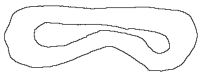
\includegraphics[interpolate=true,width=2.000000in,height=0.740000in]{contents/chapt7/figs/model/unknown_mass_trajs_3-img1.png}}%
\end{pgfscope}%
\begin{pgfscope}%
\pgfpathrectangle{\pgfqpoint{3.277208in}{3.950574in}}{\pgfqpoint{1.996630in}{0.737217in}}%
\pgfusepath{clip}%
\pgfsetbuttcap%
\pgfsetroundjoin%
\pgfsetlinewidth{1.505625pt}%
\definecolor{currentstroke}{rgb}{1.000000,0.000000,0.000000}%
\pgfsetstrokecolor{currentstroke}%
\pgfsetdash{{1.500000pt}{2.475000pt}}{0.000000pt}%
\pgfpathmoveto{\pgfqpoint{4.501540in}{4.384629in}}%
\pgfpathlineto{\pgfqpoint{4.501540in}{4.630368in}}%
\pgfusepath{stroke}%
\end{pgfscope}%
\begin{pgfscope}%
\pgfpathrectangle{\pgfqpoint{3.277208in}{3.950574in}}{\pgfqpoint{1.996630in}{0.737217in}}%
\pgfusepath{clip}%
\pgfsetrectcap%
\pgfsetroundjoin%
\pgfsetlinewidth{1.505625pt}%
\definecolor{currentstroke}{rgb}{0.121569,0.466667,0.705882}%
\pgfsetstrokecolor{currentstroke}%
\pgfsetstrokeopacity{0.700000}%
\pgfsetdash{}{0pt}%
\pgfpathmoveto{\pgfqpoint{4.505904in}{4.503487in}}%
\pgfpathlineto{\pgfqpoint{4.454214in}{4.504519in}}%
\pgfpathlineto{\pgfqpoint{4.412899in}{4.507536in}}%
\pgfpathlineto{\pgfqpoint{4.269619in}{4.520713in}}%
\pgfpathlineto{\pgfqpoint{4.209513in}{4.522315in}}%
\pgfpathlineto{\pgfqpoint{4.136442in}{4.522092in}}%
\pgfpathlineto{\pgfqpoint{4.075096in}{4.519707in}}%
\pgfpathlineto{\pgfqpoint{4.013843in}{4.514965in}}%
\pgfpathlineto{\pgfqpoint{3.946833in}{4.507607in}}%
\pgfpathlineto{\pgfqpoint{3.727420in}{4.479141in}}%
\pgfpathlineto{\pgfqpoint{3.691218in}{4.472313in}}%
\pgfpathlineto{\pgfqpoint{3.661532in}{4.464457in}}%
\pgfpathlineto{\pgfqpoint{3.638381in}{4.456274in}}%
\pgfpathlineto{\pgfqpoint{3.616076in}{4.446061in}}%
\pgfpathlineto{\pgfqpoint{3.594972in}{4.433575in}}%
\pgfpathlineto{\pgfqpoint{3.575475in}{4.418745in}}%
\pgfpathlineto{\pgfqpoint{3.562164in}{4.406038in}}%
\pgfpathlineto{\pgfqpoint{3.550210in}{4.392066in}}%
\pgfpathlineto{\pgfqpoint{3.539781in}{4.376935in}}%
\pgfpathlineto{\pgfqpoint{3.531024in}{4.360739in}}%
\pgfpathlineto{\pgfqpoint{3.524077in}{4.343677in}}%
\pgfpathlineto{\pgfqpoint{3.519087in}{4.325929in}}%
\pgfpathlineto{\pgfqpoint{3.516174in}{4.307734in}}%
\pgfpathlineto{\pgfqpoint{3.515336in}{4.289320in}}%
\pgfpathlineto{\pgfqpoint{3.516618in}{4.270922in}}%
\pgfpathlineto{\pgfqpoint{3.519996in}{4.252801in}}%
\pgfpathlineto{\pgfqpoint{3.525441in}{4.235190in}}%
\pgfpathlineto{\pgfqpoint{3.532863in}{4.218327in}}%
\pgfpathlineto{\pgfqpoint{3.542157in}{4.202460in}}%
\pgfpathlineto{\pgfqpoint{3.553155in}{4.187755in}}%
\pgfpathlineto{\pgfqpoint{3.565671in}{4.174306in}}%
\pgfpathlineto{\pgfqpoint{3.579521in}{4.162247in}}%
\pgfpathlineto{\pgfqpoint{3.594523in}{4.151667in}}%
\pgfpathlineto{\pgfqpoint{3.610505in}{4.142602in}}%
\pgfpathlineto{\pgfqpoint{3.627272in}{4.135117in}}%
\pgfpathlineto{\pgfqpoint{3.650533in}{4.127565in}}%
\pgfpathlineto{\pgfqpoint{3.674449in}{4.122596in}}%
\pgfpathlineto{\pgfqpoint{3.698867in}{4.120030in}}%
\pgfpathlineto{\pgfqpoint{3.723431in}{4.119676in}}%
\pgfpathlineto{\pgfqpoint{3.747943in}{4.121343in}}%
\pgfpathlineto{\pgfqpoint{3.772194in}{4.124899in}}%
\pgfpathlineto{\pgfqpoint{3.802159in}{4.131509in}}%
\pgfpathlineto{\pgfqpoint{3.849535in}{4.144618in}}%
\pgfpathlineto{\pgfqpoint{3.944185in}{4.171263in}}%
\pgfpathlineto{\pgfqpoint{4.199112in}{4.237500in}}%
\pgfpathlineto{\pgfqpoint{4.241450in}{4.244772in}}%
\pgfpathlineto{\pgfqpoint{4.278069in}{4.248912in}}%
\pgfpathlineto{\pgfqpoint{4.314820in}{4.250875in}}%
\pgfpathlineto{\pgfqpoint{4.351629in}{4.250314in}}%
\pgfpathlineto{\pgfqpoint{4.382261in}{4.247800in}}%
\pgfpathlineto{\pgfqpoint{4.418733in}{4.242450in}}%
\pgfpathlineto{\pgfqpoint{4.454751in}{4.234617in}}%
\pgfpathlineto{\pgfqpoint{4.490083in}{4.224201in}}%
\pgfpathlineto{\pgfqpoint{4.536200in}{4.207418in}}%
\pgfpathlineto{\pgfqpoint{4.593891in}{4.186544in}}%
\pgfpathlineto{\pgfqpoint{4.635052in}{4.174015in}}%
\pgfpathlineto{\pgfqpoint{4.700361in}{4.156622in}}%
\pgfpathlineto{\pgfqpoint{4.748317in}{4.145752in}}%
\pgfpathlineto{\pgfqpoint{4.784586in}{4.139288in}}%
\pgfpathlineto{\pgfqpoint{4.815093in}{4.135660in}}%
\pgfpathlineto{\pgfqpoint{4.845758in}{4.134119in}}%
\pgfpathlineto{\pgfqpoint{4.870211in}{4.134745in}}%
\pgfpathlineto{\pgfqpoint{4.894460in}{4.137324in}}%
\pgfpathlineto{\pgfqpoint{4.918326in}{4.142065in}}%
\pgfpathlineto{\pgfqpoint{4.941530in}{4.149187in}}%
\pgfpathlineto{\pgfqpoint{4.963749in}{4.158742in}}%
\pgfpathlineto{\pgfqpoint{4.979587in}{4.167563in}}%
\pgfpathlineto{\pgfqpoint{4.994549in}{4.177814in}}%
\pgfpathlineto{\pgfqpoint{5.008509in}{4.189440in}}%
\pgfpathlineto{\pgfqpoint{5.021263in}{4.202370in}}%
\pgfpathlineto{\pgfqpoint{5.032648in}{4.216539in}}%
\pgfpathlineto{\pgfqpoint{5.042528in}{4.231830in}}%
\pgfpathlineto{\pgfqpoint{5.050753in}{4.248097in}}%
\pgfpathlineto{\pgfqpoint{5.057204in}{4.265156in}}%
\pgfpathlineto{\pgfqpoint{5.061743in}{4.282867in}}%
\pgfpathlineto{\pgfqpoint{5.064252in}{4.301009in}}%
\pgfpathlineto{\pgfqpoint{5.064714in}{4.319319in}}%
\pgfpathlineto{\pgfqpoint{5.063124in}{4.337571in}}%
\pgfpathlineto{\pgfqpoint{5.059466in}{4.355552in}}%
\pgfpathlineto{\pgfqpoint{5.053787in}{4.373051in}}%
\pgfpathlineto{\pgfqpoint{5.046161in}{4.389831in}}%
\pgfpathlineto{\pgfqpoint{5.036733in}{4.405722in}}%
\pgfpathlineto{\pgfqpoint{5.025687in}{4.420516in}}%
\pgfpathlineto{\pgfqpoint{5.013146in}{4.434049in}}%
\pgfpathlineto{\pgfqpoint{4.999263in}{4.446188in}}%
\pgfpathlineto{\pgfqpoint{4.984252in}{4.456850in}}%
\pgfpathlineto{\pgfqpoint{4.962797in}{4.468815in}}%
\pgfpathlineto{\pgfqpoint{4.940120in}{4.478198in}}%
\pgfpathlineto{\pgfqpoint{4.916619in}{4.485171in}}%
\pgfpathlineto{\pgfqpoint{4.892589in}{4.489885in}}%
\pgfpathlineto{\pgfqpoint{4.868206in}{4.492516in}}%
\pgfpathlineto{\pgfqpoint{4.837545in}{4.493639in}}%
\pgfpathlineto{\pgfqpoint{4.714776in}{4.495595in}}%
\pgfpathlineto{\pgfqpoint{4.653474in}{4.500426in}}%
\pgfpathlineto{\pgfqpoint{4.512805in}{4.514491in}}%
\pgfpathlineto{\pgfqpoint{4.512805in}{4.514491in}}%
\pgfusepath{stroke}%
\end{pgfscope}%
\begin{pgfscope}%
\pgfpathrectangle{\pgfqpoint{3.277208in}{3.950574in}}{\pgfqpoint{1.996630in}{0.737217in}}%
\pgfusepath{clip}%
\pgfsetrectcap%
\pgfsetroundjoin%
\pgfsetlinewidth{1.505625pt}%
\definecolor{currentstroke}{rgb}{1.000000,0.498039,0.054902}%
\pgfsetstrokecolor{currentstroke}%
\pgfsetstrokeopacity{0.700000}%
\pgfsetdash{}{0pt}%
\pgfpathmoveto{\pgfqpoint{4.505904in}{4.503487in}}%
\pgfpathlineto{\pgfqpoint{4.454158in}{4.504521in}}%
\pgfpathlineto{\pgfqpoint{4.412799in}{4.507529in}}%
\pgfpathlineto{\pgfqpoint{4.280893in}{4.519600in}}%
\pgfpathlineto{\pgfqpoint{4.226638in}{4.521098in}}%
\pgfpathlineto{\pgfqpoint{4.147643in}{4.520732in}}%
\pgfpathlineto{\pgfqpoint{4.080371in}{4.518309in}}%
\pgfpathlineto{\pgfqpoint{4.025265in}{4.514127in}}%
\pgfpathlineto{\pgfqpoint{3.964345in}{4.507368in}}%
\pgfpathlineto{\pgfqpoint{3.805817in}{4.488066in}}%
\pgfpathlineto{\pgfqpoint{3.707909in}{4.480573in}}%
\pgfpathlineto{\pgfqpoint{3.677601in}{4.475540in}}%
\pgfpathlineto{\pgfqpoint{3.653758in}{4.469621in}}%
\pgfpathlineto{\pgfqpoint{3.630527in}{4.461634in}}%
\pgfpathlineto{\pgfqpoint{3.608248in}{4.451324in}}%
\pgfpathlineto{\pgfqpoint{3.587298in}{4.438536in}}%
\pgfpathlineto{\pgfqpoint{3.572710in}{4.427325in}}%
\pgfpathlineto{\pgfqpoint{3.559306in}{4.414725in}}%
\pgfpathlineto{\pgfqpoint{3.547281in}{4.400781in}}%
\pgfpathlineto{\pgfqpoint{3.536803in}{4.385622in}}%
\pgfpathlineto{\pgfqpoint{3.528052in}{4.369405in}}%
\pgfpathlineto{\pgfqpoint{3.521174in}{4.352334in}}%
\pgfpathlineto{\pgfqpoint{3.516293in}{4.334588in}}%
\pgfpathlineto{\pgfqpoint{3.513491in}{4.316389in}}%
\pgfpathlineto{\pgfqpoint{3.512835in}{4.297988in}}%
\pgfpathlineto{\pgfqpoint{3.514329in}{4.279669in}}%
\pgfpathlineto{\pgfqpoint{3.517981in}{4.261665in}}%
\pgfpathlineto{\pgfqpoint{3.523718in}{4.244156in}}%
\pgfpathlineto{\pgfqpoint{3.531398in}{4.227397in}}%
\pgfpathlineto{\pgfqpoint{3.540899in}{4.211616in}}%
\pgfpathlineto{\pgfqpoint{3.552076in}{4.196980in}}%
\pgfpathlineto{\pgfqpoint{3.564726in}{4.183612in}}%
\pgfpathlineto{\pgfqpoint{3.578703in}{4.171633in}}%
\pgfpathlineto{\pgfqpoint{3.593830in}{4.161081in}}%
\pgfpathlineto{\pgfqpoint{3.609870in}{4.152007in}}%
\pgfpathlineto{\pgfqpoint{3.632425in}{4.142268in}}%
\pgfpathlineto{\pgfqpoint{3.655967in}{4.135248in}}%
\pgfpathlineto{\pgfqpoint{3.680122in}{4.130762in}}%
\pgfpathlineto{\pgfqpoint{3.704596in}{4.128669in}}%
\pgfpathlineto{\pgfqpoint{3.729168in}{4.128842in}}%
\pgfpathlineto{\pgfqpoint{3.753634in}{4.131127in}}%
\pgfpathlineto{\pgfqpoint{3.783865in}{4.136536in}}%
\pgfpathlineto{\pgfqpoint{3.819656in}{4.145429in}}%
\pgfpathlineto{\pgfqpoint{3.985839in}{4.189961in}}%
\pgfpathlineto{\pgfqpoint{4.098983in}{4.218555in}}%
\pgfpathlineto{\pgfqpoint{4.188153in}{4.241639in}}%
\pgfpathlineto{\pgfqpoint{4.224256in}{4.248995in}}%
\pgfpathlineto{\pgfqpoint{4.260745in}{4.254181in}}%
\pgfpathlineto{\pgfqpoint{4.291398in}{4.256493in}}%
\pgfpathlineto{\pgfqpoint{4.322092in}{4.256778in}}%
\pgfpathlineto{\pgfqpoint{4.352742in}{4.255090in}}%
\pgfpathlineto{\pgfqpoint{4.389330in}{4.250556in}}%
\pgfpathlineto{\pgfqpoint{4.425456in}{4.243487in}}%
\pgfpathlineto{\pgfqpoint{4.461038in}{4.234032in}}%
\pgfpathlineto{\pgfqpoint{4.495949in}{4.222317in}}%
\pgfpathlineto{\pgfqpoint{4.605288in}{4.182263in}}%
\pgfpathlineto{\pgfqpoint{4.652507in}{4.169585in}}%
\pgfpathlineto{\pgfqpoint{4.712292in}{4.156084in}}%
\pgfpathlineto{\pgfqpoint{4.766639in}{4.145846in}}%
\pgfpathlineto{\pgfqpoint{4.803196in}{4.140899in}}%
\pgfpathlineto{\pgfqpoint{4.833825in}{4.138652in}}%
\pgfpathlineto{\pgfqpoint{4.864390in}{4.138729in}}%
\pgfpathlineto{\pgfqpoint{4.888667in}{4.140874in}}%
\pgfpathlineto{\pgfqpoint{4.912543in}{4.145108in}}%
\pgfpathlineto{\pgfqpoint{4.935788in}{4.151665in}}%
\pgfpathlineto{\pgfqpoint{4.958170in}{4.160714in}}%
\pgfpathlineto{\pgfqpoint{4.979350in}{4.172292in}}%
\pgfpathlineto{\pgfqpoint{4.994196in}{4.182649in}}%
\pgfpathlineto{\pgfqpoint{5.008011in}{4.194413in}}%
\pgfpathlineto{\pgfqpoint{5.020551in}{4.207505in}}%
\pgfpathlineto{\pgfqpoint{5.031667in}{4.221851in}}%
\pgfpathlineto{\pgfqpoint{5.041172in}{4.237268in}}%
\pgfpathlineto{\pgfqpoint{5.048915in}{4.253644in}}%
\pgfpathlineto{\pgfqpoint{5.054802in}{4.270860in}}%
\pgfpathlineto{\pgfqpoint{5.058723in}{4.288667in}}%
\pgfpathlineto{\pgfqpoint{5.060631in}{4.306833in}}%
\pgfpathlineto{\pgfqpoint{5.060480in}{4.325098in}}%
\pgfpathlineto{\pgfqpoint{5.058266in}{4.343247in}}%
\pgfpathlineto{\pgfqpoint{5.053989in}{4.361077in}}%
\pgfpathlineto{\pgfqpoint{5.047762in}{4.378310in}}%
\pgfpathlineto{\pgfqpoint{5.039676in}{4.394786in}}%
\pgfpathlineto{\pgfqpoint{5.029828in}{4.410295in}}%
\pgfpathlineto{\pgfqpoint{5.018368in}{4.424652in}}%
\pgfpathlineto{\pgfqpoint{5.005412in}{4.437746in}}%
\pgfpathlineto{\pgfqpoint{4.991189in}{4.449468in}}%
\pgfpathlineto{\pgfqpoint{4.975888in}{4.459707in}}%
\pgfpathlineto{\pgfqpoint{4.954145in}{4.471138in}}%
\pgfpathlineto{\pgfqpoint{4.931268in}{4.480153in}}%
\pgfpathlineto{\pgfqpoint{4.907645in}{4.486934in}}%
\pgfpathlineto{\pgfqpoint{4.883565in}{4.491669in}}%
\pgfpathlineto{\pgfqpoint{4.853039in}{4.495029in}}%
\pgfpathlineto{\pgfqpoint{4.810127in}{4.496697in}}%
\pgfpathlineto{\pgfqpoint{4.705694in}{4.499216in}}%
\pgfpathlineto{\pgfqpoint{4.638262in}{4.503637in}}%
\pgfpathlineto{\pgfqpoint{4.503734in}{4.515379in}}%
\pgfpathlineto{\pgfqpoint{4.503734in}{4.515379in}}%
\pgfusepath{stroke}%
\end{pgfscope}%
\begin{pgfscope}%
\pgfsetbuttcap%
\pgfsetmiterjoin%
\definecolor{currentfill}{rgb}{1.000000,1.000000,1.000000}%
\pgfsetfillcolor{currentfill}%
\pgfsetlinewidth{1.003750pt}%
\definecolor{currentstroke}{rgb}{0.000000,0.000000,0.000000}%
\pgfsetstrokecolor{currentstroke}%
\pgfsetdash{}{0pt}%
\pgfpathmoveto{\pgfqpoint{3.741607in}{4.503820in}}%
\pgfpathlineto{\pgfqpoint{3.998756in}{4.503820in}}%
\pgfpathquadraticcurveto{\pgfqpoint{4.010325in}{4.503820in}}{\pgfqpoint{4.010325in}{4.515389in}}%
\pgfpathlineto{\pgfqpoint{4.010325in}{4.627355in}}%
\pgfpathquadraticcurveto{\pgfqpoint{4.010325in}{4.638924in}}{\pgfqpoint{3.998756in}{4.638924in}}%
\pgfpathlineto{\pgfqpoint{3.741607in}{4.638924in}}%
\pgfpathquadraticcurveto{\pgfqpoint{3.730037in}{4.638924in}}{\pgfqpoint{3.730037in}{4.627355in}}%
\pgfpathlineto{\pgfqpoint{3.730037in}{4.515389in}}%
\pgfpathquadraticcurveto{\pgfqpoint{3.730037in}{4.503820in}}{\pgfqpoint{3.741607in}{4.503820in}}%
\pgfpathlineto{\pgfqpoint{3.741607in}{4.503820in}}%
\pgfpathclose%
\pgfusepath{stroke,fill}%
\end{pgfscope}%
\begin{pgfscope}%
\definecolor{textcolor}{rgb}{0.000000,0.000000,0.000000}%
\pgfsetstrokecolor{textcolor}%
\pgfsetfillcolor{textcolor}%
\pgftext[x=3.741607in,y=4.539454in,left,base]{\color{textcolor}\rmfamily\fontsize{8.330000}{9.996000}\selectfont 20\%}%
\end{pgfscope}%
\begin{pgfscope}%
\pgfsetbuttcap%
\pgfsetmiterjoin%
\definecolor{currentfill}{rgb}{1.000000,1.000000,1.000000}%
\pgfsetfillcolor{currentfill}%
\pgfsetlinewidth{1.003750pt}%
\definecolor{currentstroke}{rgb}{0.000000,0.000000,0.000000}%
\pgfsetstrokecolor{currentstroke}%
\pgfsetdash{}{0pt}%
\pgfpathmoveto{\pgfqpoint{3.739265in}{4.087225in}}%
\pgfpathlineto{\pgfqpoint{3.996414in}{4.087225in}}%
\pgfpathquadraticcurveto{\pgfqpoint{4.007983in}{4.087225in}}{\pgfqpoint{4.007983in}{4.098794in}}%
\pgfpathlineto{\pgfqpoint{4.007983in}{4.210760in}}%
\pgfpathquadraticcurveto{\pgfqpoint{4.007983in}{4.222329in}}{\pgfqpoint{3.996414in}{4.222329in}}%
\pgfpathlineto{\pgfqpoint{3.739265in}{4.222329in}}%
\pgfpathquadraticcurveto{\pgfqpoint{3.727695in}{4.222329in}}{\pgfqpoint{3.727695in}{4.210760in}}%
\pgfpathlineto{\pgfqpoint{3.727695in}{4.098794in}}%
\pgfpathquadraticcurveto{\pgfqpoint{3.727695in}{4.087225in}}{\pgfqpoint{3.739265in}{4.087225in}}%
\pgfpathlineto{\pgfqpoint{3.739265in}{4.087225in}}%
\pgfpathclose%
\pgfusepath{stroke,fill}%
\end{pgfscope}%
\begin{pgfscope}%
\definecolor{textcolor}{rgb}{0.000000,0.000000,0.000000}%
\pgfsetstrokecolor{textcolor}%
\pgfsetfillcolor{textcolor}%
\pgftext[x=3.739265in,y=4.122859in,left,base]{\color{textcolor}\rmfamily\fontsize{8.330000}{9.996000}\selectfont 40\%}%
\end{pgfscope}%
\begin{pgfscope}%
\pgfsetbuttcap%
\pgfsetmiterjoin%
\definecolor{currentfill}{rgb}{1.000000,1.000000,1.000000}%
\pgfsetfillcolor{currentfill}%
\pgfsetlinewidth{1.003750pt}%
\definecolor{currentstroke}{rgb}{0.000000,0.000000,0.000000}%
\pgfsetstrokecolor{currentstroke}%
\pgfsetdash{}{0pt}%
\pgfpathmoveto{\pgfqpoint{4.466369in}{4.248009in}}%
\pgfpathlineto{\pgfqpoint{4.723517in}{4.248009in}}%
\pgfpathquadraticcurveto{\pgfqpoint{4.735087in}{4.248009in}}{\pgfqpoint{4.735087in}{4.259579in}}%
\pgfpathlineto{\pgfqpoint{4.735087in}{4.371545in}}%
\pgfpathquadraticcurveto{\pgfqpoint{4.735087in}{4.383114in}}{\pgfqpoint{4.723517in}{4.383114in}}%
\pgfpathlineto{\pgfqpoint{4.466369in}{4.383114in}}%
\pgfpathquadraticcurveto{\pgfqpoint{4.454799in}{4.383114in}}{\pgfqpoint{4.454799in}{4.371545in}}%
\pgfpathlineto{\pgfqpoint{4.454799in}{4.259579in}}%
\pgfpathquadraticcurveto{\pgfqpoint{4.454799in}{4.248009in}}{\pgfqpoint{4.466369in}{4.248009in}}%
\pgfpathlineto{\pgfqpoint{4.466369in}{4.248009in}}%
\pgfpathclose%
\pgfusepath{stroke,fill}%
\end{pgfscope}%
\begin{pgfscope}%
\definecolor{textcolor}{rgb}{0.000000,0.000000,0.000000}%
\pgfsetstrokecolor{textcolor}%
\pgfsetfillcolor{textcolor}%
\pgftext[x=4.466369in,y=4.283644in,left,base]{\color{textcolor}\rmfamily\fontsize{8.330000}{9.996000}\selectfont 60\%}%
\end{pgfscope}%
\begin{pgfscope}%
\pgfsetbuttcap%
\pgfsetmiterjoin%
\definecolor{currentfill}{rgb}{1.000000,1.000000,1.000000}%
\pgfsetfillcolor{currentfill}%
\pgfsetlinewidth{1.003750pt}%
\definecolor{currentstroke}{rgb}{0.000000,0.000000,0.000000}%
\pgfsetstrokecolor{currentstroke}%
\pgfsetdash{}{0pt}%
\pgfpathmoveto{\pgfqpoint{5.086966in}{4.193809in}}%
\pgfpathlineto{\pgfqpoint{5.344115in}{4.193809in}}%
\pgfpathquadraticcurveto{\pgfqpoint{5.355684in}{4.193809in}}{\pgfqpoint{5.355684in}{4.205378in}}%
\pgfpathlineto{\pgfqpoint{5.355684in}{4.317344in}}%
\pgfpathquadraticcurveto{\pgfqpoint{5.355684in}{4.328914in}}{\pgfqpoint{5.344115in}{4.328914in}}%
\pgfpathlineto{\pgfqpoint{5.086966in}{4.328914in}}%
\pgfpathquadraticcurveto{\pgfqpoint{5.075396in}{4.328914in}}{\pgfqpoint{5.075396in}{4.317344in}}%
\pgfpathlineto{\pgfqpoint{5.075396in}{4.205378in}}%
\pgfpathquadraticcurveto{\pgfqpoint{5.075396in}{4.193809in}}{\pgfqpoint{5.086966in}{4.193809in}}%
\pgfpathlineto{\pgfqpoint{5.086966in}{4.193809in}}%
\pgfpathclose%
\pgfusepath{stroke,fill}%
\end{pgfscope}%
\begin{pgfscope}%
\definecolor{textcolor}{rgb}{0.000000,0.000000,0.000000}%
\pgfsetstrokecolor{textcolor}%
\pgfsetfillcolor{textcolor}%
\pgftext[x=5.086966in,y=4.229444in,left,base]{\color{textcolor}\rmfamily\fontsize{8.330000}{9.996000}\selectfont 80\%}%
\end{pgfscope}%
\begin{pgfscope}%
\definecolor{textcolor}{rgb}{0.000000,0.000000,0.000000}%
\pgfsetstrokecolor{textcolor}%
\pgfsetfillcolor{textcolor}%
\pgftext[x=4.275523in,y=4.771125in,,base]{\color{textcolor}\rmfamily\fontsize{12.000000}{14.400000}\selectfont Steering and velocity control}%
\end{pgfscope}%
\begin{pgfscope}%
\pgfsetbuttcap%
\pgfsetmiterjoin%
\definecolor{currentfill}{rgb}{1.000000,1.000000,1.000000}%
\pgfsetfillcolor{currentfill}%
\pgfsetlinewidth{0.000000pt}%
\definecolor{currentstroke}{rgb}{0.000000,0.000000,0.000000}%
\pgfsetstrokecolor{currentstroke}%
\pgfsetstrokeopacity{0.000000}%
\pgfsetdash{}{0pt}%
\pgfpathmoveto{\pgfqpoint{1.054417in}{2.960609in}}%
\pgfpathlineto{\pgfqpoint{3.051047in}{2.960609in}}%
\pgfpathlineto{\pgfqpoint{3.051047in}{3.717148in}}%
\pgfpathlineto{\pgfqpoint{1.054417in}{3.717148in}}%
\pgfpathlineto{\pgfqpoint{1.054417in}{2.960609in}}%
\pgfpathclose%
\pgfusepath{fill}%
\end{pgfscope}%
\begin{pgfscope}%
\pgfpathrectangle{\pgfqpoint{1.054417in}{2.960609in}}{\pgfqpoint{1.996630in}{0.756539in}}%
\pgfusepath{clip}%
\pgfsetrectcap%
\pgfsetroundjoin%
\pgfsetlinewidth{0.803000pt}%
\definecolor{currentstroke}{rgb}{0.690196,0.690196,0.690196}%
\pgfsetstrokecolor{currentstroke}%
\pgfsetdash{}{0pt}%
\pgfpathmoveto{\pgfqpoint{1.145173in}{2.960609in}}%
\pgfpathlineto{\pgfqpoint{1.145173in}{3.717148in}}%
\pgfusepath{stroke}%
\end{pgfscope}%
\begin{pgfscope}%
\pgfpathrectangle{\pgfqpoint{1.054417in}{2.960609in}}{\pgfqpoint{1.996630in}{0.756539in}}%
\pgfusepath{clip}%
\pgfsetrectcap%
\pgfsetroundjoin%
\pgfsetlinewidth{0.803000pt}%
\definecolor{currentstroke}{rgb}{0.690196,0.690196,0.690196}%
\pgfsetstrokecolor{currentstroke}%
\pgfsetdash{}{0pt}%
\pgfpathmoveto{\pgfqpoint{1.509379in}{2.960609in}}%
\pgfpathlineto{\pgfqpoint{1.509379in}{3.717148in}}%
\pgfusepath{stroke}%
\end{pgfscope}%
\begin{pgfscope}%
\pgfpathrectangle{\pgfqpoint{1.054417in}{2.960609in}}{\pgfqpoint{1.996630in}{0.756539in}}%
\pgfusepath{clip}%
\pgfsetrectcap%
\pgfsetroundjoin%
\pgfsetlinewidth{0.803000pt}%
\definecolor{currentstroke}{rgb}{0.690196,0.690196,0.690196}%
\pgfsetstrokecolor{currentstroke}%
\pgfsetdash{}{0pt}%
\pgfpathmoveto{\pgfqpoint{1.873585in}{2.960609in}}%
\pgfpathlineto{\pgfqpoint{1.873585in}{3.717148in}}%
\pgfusepath{stroke}%
\end{pgfscope}%
\begin{pgfscope}%
\pgfpathrectangle{\pgfqpoint{1.054417in}{2.960609in}}{\pgfqpoint{1.996630in}{0.756539in}}%
\pgfusepath{clip}%
\pgfsetrectcap%
\pgfsetroundjoin%
\pgfsetlinewidth{0.803000pt}%
\definecolor{currentstroke}{rgb}{0.690196,0.690196,0.690196}%
\pgfsetstrokecolor{currentstroke}%
\pgfsetdash{}{0pt}%
\pgfpathmoveto{\pgfqpoint{2.237791in}{2.960609in}}%
\pgfpathlineto{\pgfqpoint{2.237791in}{3.717148in}}%
\pgfusepath{stroke}%
\end{pgfscope}%
\begin{pgfscope}%
\pgfpathrectangle{\pgfqpoint{1.054417in}{2.960609in}}{\pgfqpoint{1.996630in}{0.756539in}}%
\pgfusepath{clip}%
\pgfsetrectcap%
\pgfsetroundjoin%
\pgfsetlinewidth{0.803000pt}%
\definecolor{currentstroke}{rgb}{0.690196,0.690196,0.690196}%
\pgfsetstrokecolor{currentstroke}%
\pgfsetdash{}{0pt}%
\pgfpathmoveto{\pgfqpoint{2.601997in}{2.960609in}}%
\pgfpathlineto{\pgfqpoint{2.601997in}{3.717148in}}%
\pgfusepath{stroke}%
\end{pgfscope}%
\begin{pgfscope}%
\pgfpathrectangle{\pgfqpoint{1.054417in}{2.960609in}}{\pgfqpoint{1.996630in}{0.756539in}}%
\pgfusepath{clip}%
\pgfsetrectcap%
\pgfsetroundjoin%
\pgfsetlinewidth{0.803000pt}%
\definecolor{currentstroke}{rgb}{0.690196,0.690196,0.690196}%
\pgfsetstrokecolor{currentstroke}%
\pgfsetdash{}{0pt}%
\pgfpathmoveto{\pgfqpoint{2.966203in}{2.960609in}}%
\pgfpathlineto{\pgfqpoint{2.966203in}{3.717148in}}%
\pgfusepath{stroke}%
\end{pgfscope}%
\begin{pgfscope}%
\pgfpathrectangle{\pgfqpoint{1.054417in}{2.960609in}}{\pgfqpoint{1.996630in}{0.756539in}}%
\pgfusepath{clip}%
\pgfsetrectcap%
\pgfsetroundjoin%
\pgfsetlinewidth{0.803000pt}%
\definecolor{currentstroke}{rgb}{0.690196,0.690196,0.690196}%
\pgfsetstrokecolor{currentstroke}%
\pgfsetdash{}{0pt}%
\pgfpathmoveto{\pgfqpoint{1.054417in}{2.981771in}}%
\pgfpathlineto{\pgfqpoint{3.051047in}{2.981771in}}%
\pgfusepath{stroke}%
\end{pgfscope}%
\begin{pgfscope}%
\definecolor{textcolor}{rgb}{0.000000,0.000000,0.000000}%
\pgfsetstrokecolor{textcolor}%
\pgfsetfillcolor{textcolor}%
\pgftext[x=0.676901in, y=2.929009in, left, base]{\color{textcolor}\rmfamily\fontsize{10.000000}{12.000000}\selectfont \ensuremath{-}0.4}%
\end{pgfscope}%
\begin{pgfscope}%
\pgfpathrectangle{\pgfqpoint{1.054417in}{2.960609in}}{\pgfqpoint{1.996630in}{0.756539in}}%
\pgfusepath{clip}%
\pgfsetrectcap%
\pgfsetroundjoin%
\pgfsetlinewidth{0.803000pt}%
\definecolor{currentstroke}{rgb}{0.690196,0.690196,0.690196}%
\pgfsetstrokecolor{currentstroke}%
\pgfsetdash{}{0pt}%
\pgfpathmoveto{\pgfqpoint{1.054417in}{3.312426in}}%
\pgfpathlineto{\pgfqpoint{3.051047in}{3.312426in}}%
\pgfusepath{stroke}%
\end{pgfscope}%
\begin{pgfscope}%
\definecolor{textcolor}{rgb}{0.000000,0.000000,0.000000}%
\pgfsetstrokecolor{textcolor}%
\pgfsetfillcolor{textcolor}%
\pgftext[x=0.784926in, y=3.259665in, left, base]{\color{textcolor}\rmfamily\fontsize{10.000000}{12.000000}\selectfont 0.0}%
\end{pgfscope}%
\begin{pgfscope}%
\pgfpathrectangle{\pgfqpoint{1.054417in}{2.960609in}}{\pgfqpoint{1.996630in}{0.756539in}}%
\pgfusepath{clip}%
\pgfsetrectcap%
\pgfsetroundjoin%
\pgfsetlinewidth{0.803000pt}%
\definecolor{currentstroke}{rgb}{0.690196,0.690196,0.690196}%
\pgfsetstrokecolor{currentstroke}%
\pgfsetdash{}{0pt}%
\pgfpathmoveto{\pgfqpoint{1.054417in}{3.643081in}}%
\pgfpathlineto{\pgfqpoint{3.051047in}{3.643081in}}%
\pgfusepath{stroke}%
\end{pgfscope}%
\begin{pgfscope}%
\definecolor{textcolor}{rgb}{0.000000,0.000000,0.000000}%
\pgfsetstrokecolor{textcolor}%
\pgfsetfillcolor{textcolor}%
\pgftext[x=0.784926in, y=3.590320in, left, base]{\color{textcolor}\rmfamily\fontsize{10.000000}{12.000000}\selectfont 0.4}%
\end{pgfscope}%
\begin{pgfscope}%
\definecolor{textcolor}{rgb}{0.000000,0.000000,0.000000}%
\pgfsetstrokecolor{textcolor}%
\pgfsetfillcolor{textcolor}%
\pgftext[x=0.277488in, y=3.014544in, left, base,rotate=90.000000]{\color{textcolor}\rmfamily\fontsize{10.000000}{12.000000}\selectfont Steering }%
\end{pgfscope}%
\begin{pgfscope}%
\definecolor{textcolor}{rgb}{0.000000,0.000000,0.000000}%
\pgfsetstrokecolor{textcolor}%
\pgfsetfillcolor{textcolor}%
\pgftext[x=0.434972in, y=3.122916in, left, base,rotate=90.000000]{\color{textcolor}\rmfamily\fontsize{10.000000}{12.000000}\selectfont angle }%
\end{pgfscope}%
\begin{pgfscope}%
\definecolor{textcolor}{rgb}{0.000000,0.000000,0.000000}%
\pgfsetstrokecolor{textcolor}%
\pgfsetfillcolor{textcolor}%
\pgftext[x=0.592456in, y=3.130003in, left, base,rotate=90.000000]{\color{textcolor}\rmfamily\fontsize{10.000000}{12.000000}\selectfont [rads]}%
\end{pgfscope}%
\begin{pgfscope}%
\pgfpathrectangle{\pgfqpoint{1.054417in}{2.960609in}}{\pgfqpoint{1.996630in}{0.756539in}}%
\pgfusepath{clip}%
\pgfsetrectcap%
\pgfsetroundjoin%
\pgfsetlinewidth{1.505625pt}%
\definecolor{currentstroke}{rgb}{0.121569,0.466667,0.705882}%
\pgfsetstrokecolor{currentstroke}%
\pgfsetstrokeopacity{0.700000}%
\pgfsetdash{}{0pt}%
\pgfpathmoveto{\pgfqpoint{1.145173in}{3.312426in}}%
\pgfpathlineto{\pgfqpoint{1.145173in}{3.259521in}}%
\pgfpathlineto{\pgfqpoint{1.151085in}{3.233069in}}%
\pgfpathlineto{\pgfqpoint{1.151085in}{3.180164in}}%
\pgfpathlineto{\pgfqpoint{1.151085in}{3.206616in}}%
\pgfpathlineto{\pgfqpoint{1.156997in}{3.180164in}}%
\pgfpathlineto{\pgfqpoint{1.156997in}{3.206616in}}%
\pgfpathlineto{\pgfqpoint{1.156997in}{3.180164in}}%
\pgfpathlineto{\pgfqpoint{1.162910in}{3.206616in}}%
\pgfpathlineto{\pgfqpoint{1.162910in}{3.180164in}}%
\pgfpathlineto{\pgfqpoint{1.162910in}{3.206616in}}%
\pgfpathlineto{\pgfqpoint{1.168822in}{3.180164in}}%
\pgfpathlineto{\pgfqpoint{1.168822in}{3.206616in}}%
\pgfpathlineto{\pgfqpoint{1.168822in}{3.180164in}}%
\pgfpathlineto{\pgfqpoint{1.174735in}{3.206616in}}%
\pgfpathlineto{\pgfqpoint{1.174735in}{3.180164in}}%
\pgfpathlineto{\pgfqpoint{1.174735in}{3.206616in}}%
\pgfpathlineto{\pgfqpoint{1.180647in}{3.180164in}}%
\pgfpathlineto{\pgfqpoint{1.180647in}{3.233069in}}%
\pgfpathlineto{\pgfqpoint{1.186560in}{3.259521in}}%
\pgfpathlineto{\pgfqpoint{1.186560in}{3.312426in}}%
\pgfpathlineto{\pgfqpoint{1.192472in}{3.338879in}}%
\pgfpathlineto{\pgfqpoint{1.192472in}{3.391783in}}%
\pgfpathlineto{\pgfqpoint{1.198385in}{3.365331in}}%
\pgfpathlineto{\pgfqpoint{1.198385in}{3.391783in}}%
\pgfpathlineto{\pgfqpoint{1.204297in}{3.365331in}}%
\pgfpathlineto{\pgfqpoint{1.204297in}{3.391783in}}%
\pgfpathlineto{\pgfqpoint{1.204297in}{3.365331in}}%
\pgfpathlineto{\pgfqpoint{1.210209in}{3.391783in}}%
\pgfpathlineto{\pgfqpoint{1.210209in}{3.365331in}}%
\pgfpathlineto{\pgfqpoint{1.216122in}{3.391783in}}%
\pgfpathlineto{\pgfqpoint{1.216122in}{3.365331in}}%
\pgfpathlineto{\pgfqpoint{1.216122in}{3.391783in}}%
\pgfpathlineto{\pgfqpoint{1.222034in}{3.365331in}}%
\pgfpathlineto{\pgfqpoint{1.222034in}{3.391783in}}%
\pgfpathlineto{\pgfqpoint{1.227947in}{3.365331in}}%
\pgfpathlineto{\pgfqpoint{1.227947in}{3.391783in}}%
\pgfpathlineto{\pgfqpoint{1.227947in}{3.365331in}}%
\pgfpathlineto{\pgfqpoint{1.233859in}{3.391783in}}%
\pgfpathlineto{\pgfqpoint{1.233859in}{3.365331in}}%
\pgfpathlineto{\pgfqpoint{1.239772in}{3.391783in}}%
\pgfpathlineto{\pgfqpoint{1.239772in}{3.365331in}}%
\pgfpathlineto{\pgfqpoint{1.245684in}{3.391783in}}%
\pgfpathlineto{\pgfqpoint{1.245684in}{3.365331in}}%
\pgfpathlineto{\pgfqpoint{1.251596in}{3.391783in}}%
\pgfpathlineto{\pgfqpoint{1.251596in}{3.365331in}}%
\pgfpathlineto{\pgfqpoint{1.257509in}{3.391783in}}%
\pgfpathlineto{\pgfqpoint{1.257509in}{3.365331in}}%
\pgfpathlineto{\pgfqpoint{1.257509in}{3.391783in}}%
\pgfpathlineto{\pgfqpoint{1.263421in}{3.365331in}}%
\pgfpathlineto{\pgfqpoint{1.263421in}{3.391783in}}%
\pgfpathlineto{\pgfqpoint{1.269334in}{3.365331in}}%
\pgfpathlineto{\pgfqpoint{1.269334in}{3.391783in}}%
\pgfpathlineto{\pgfqpoint{1.275246in}{3.365331in}}%
\pgfpathlineto{\pgfqpoint{1.275246in}{3.391783in}}%
\pgfpathlineto{\pgfqpoint{1.281159in}{3.365331in}}%
\pgfpathlineto{\pgfqpoint{1.281159in}{3.338879in}}%
\pgfpathlineto{\pgfqpoint{1.287071in}{3.312426in}}%
\pgfpathlineto{\pgfqpoint{1.287071in}{3.285974in}}%
\pgfpathlineto{\pgfqpoint{1.292984in}{3.259521in}}%
\pgfpathlineto{\pgfqpoint{1.292984in}{3.285974in}}%
\pgfpathlineto{\pgfqpoint{1.298896in}{3.259521in}}%
\pgfpathlineto{\pgfqpoint{1.298896in}{3.285974in}}%
\pgfpathlineto{\pgfqpoint{1.304808in}{3.259521in}}%
\pgfpathlineto{\pgfqpoint{1.304808in}{3.285974in}}%
\pgfpathlineto{\pgfqpoint{1.310721in}{3.259521in}}%
\pgfpathlineto{\pgfqpoint{1.310721in}{3.285974in}}%
\pgfpathlineto{\pgfqpoint{1.316633in}{3.259521in}}%
\pgfpathlineto{\pgfqpoint{1.316633in}{3.285974in}}%
\pgfpathlineto{\pgfqpoint{1.322546in}{3.259521in}}%
\pgfpathlineto{\pgfqpoint{1.322546in}{3.285974in}}%
\pgfpathlineto{\pgfqpoint{1.328458in}{3.259521in}}%
\pgfpathlineto{\pgfqpoint{1.328458in}{3.285974in}}%
\pgfpathlineto{\pgfqpoint{1.334371in}{3.259521in}}%
\pgfpathlineto{\pgfqpoint{1.334371in}{3.285974in}}%
\pgfpathlineto{\pgfqpoint{1.340283in}{3.259521in}}%
\pgfpathlineto{\pgfqpoint{1.340283in}{3.285974in}}%
\pgfpathlineto{\pgfqpoint{1.346195in}{3.312426in}}%
\pgfpathlineto{\pgfqpoint{1.346195in}{3.338879in}}%
\pgfpathlineto{\pgfqpoint{1.352108in}{3.312426in}}%
\pgfpathlineto{\pgfqpoint{1.352108in}{3.338879in}}%
\pgfpathlineto{\pgfqpoint{1.358020in}{3.312426in}}%
\pgfpathlineto{\pgfqpoint{1.358020in}{3.338879in}}%
\pgfpathlineto{\pgfqpoint{1.363933in}{3.312426in}}%
\pgfpathlineto{\pgfqpoint{1.369845in}{3.338879in}}%
\pgfpathlineto{\pgfqpoint{1.369845in}{3.312426in}}%
\pgfpathlineto{\pgfqpoint{1.375758in}{3.338879in}}%
\pgfpathlineto{\pgfqpoint{1.375758in}{3.312426in}}%
\pgfpathlineto{\pgfqpoint{1.381670in}{3.338879in}}%
\pgfpathlineto{\pgfqpoint{1.381670in}{3.312426in}}%
\pgfpathlineto{\pgfqpoint{1.387583in}{3.338879in}}%
\pgfpathlineto{\pgfqpoint{1.387583in}{3.312426in}}%
\pgfpathlineto{\pgfqpoint{1.393495in}{3.338879in}}%
\pgfpathlineto{\pgfqpoint{1.393495in}{3.312426in}}%
\pgfpathlineto{\pgfqpoint{1.399407in}{3.338879in}}%
\pgfpathlineto{\pgfqpoint{1.399407in}{3.312426in}}%
\pgfpathlineto{\pgfqpoint{1.405320in}{3.338879in}}%
\pgfpathlineto{\pgfqpoint{1.405320in}{3.312426in}}%
\pgfpathlineto{\pgfqpoint{1.411232in}{3.338879in}}%
\pgfpathlineto{\pgfqpoint{1.411232in}{3.312426in}}%
\pgfpathlineto{\pgfqpoint{1.417145in}{3.338879in}}%
\pgfpathlineto{\pgfqpoint{1.417145in}{3.312426in}}%
\pgfpathlineto{\pgfqpoint{1.423057in}{3.338879in}}%
\pgfpathlineto{\pgfqpoint{1.423057in}{3.312426in}}%
\pgfpathlineto{\pgfqpoint{1.428970in}{3.338879in}}%
\pgfpathlineto{\pgfqpoint{1.428970in}{3.312426in}}%
\pgfpathlineto{\pgfqpoint{1.434882in}{3.338879in}}%
\pgfpathlineto{\pgfqpoint{1.434882in}{3.312426in}}%
\pgfpathlineto{\pgfqpoint{1.440794in}{3.338879in}}%
\pgfpathlineto{\pgfqpoint{1.440794in}{3.312426in}}%
\pgfpathlineto{\pgfqpoint{1.446707in}{3.338879in}}%
\pgfpathlineto{\pgfqpoint{1.446707in}{3.312426in}}%
\pgfpathlineto{\pgfqpoint{1.452619in}{3.338879in}}%
\pgfpathlineto{\pgfqpoint{1.452619in}{3.312426in}}%
\pgfpathlineto{\pgfqpoint{1.458532in}{3.338879in}}%
\pgfpathlineto{\pgfqpoint{1.458532in}{3.312426in}}%
\pgfpathlineto{\pgfqpoint{1.464444in}{3.338879in}}%
\pgfpathlineto{\pgfqpoint{1.464444in}{3.365331in}}%
\pgfpathlineto{\pgfqpoint{1.470357in}{3.391783in}}%
\pgfpathlineto{\pgfqpoint{1.470357in}{3.418236in}}%
\pgfpathlineto{\pgfqpoint{1.476269in}{3.391783in}}%
\pgfpathlineto{\pgfqpoint{1.476269in}{3.418236in}}%
\pgfpathlineto{\pgfqpoint{1.482182in}{3.391783in}}%
\pgfpathlineto{\pgfqpoint{1.482182in}{3.418236in}}%
\pgfpathlineto{\pgfqpoint{1.488094in}{3.391783in}}%
\pgfpathlineto{\pgfqpoint{1.488094in}{3.418236in}}%
\pgfpathlineto{\pgfqpoint{1.494006in}{3.391783in}}%
\pgfpathlineto{\pgfqpoint{1.494006in}{3.418236in}}%
\pgfpathlineto{\pgfqpoint{1.499919in}{3.391783in}}%
\pgfpathlineto{\pgfqpoint{1.499919in}{3.418236in}}%
\pgfpathlineto{\pgfqpoint{1.505831in}{3.391783in}}%
\pgfpathlineto{\pgfqpoint{1.505831in}{3.418236in}}%
\pgfpathlineto{\pgfqpoint{1.511744in}{3.391783in}}%
\pgfpathlineto{\pgfqpoint{1.511744in}{3.418236in}}%
\pgfpathlineto{\pgfqpoint{1.517656in}{3.391783in}}%
\pgfpathlineto{\pgfqpoint{1.517656in}{3.418236in}}%
\pgfpathlineto{\pgfqpoint{1.523569in}{3.444688in}}%
\pgfpathlineto{\pgfqpoint{1.523569in}{3.418236in}}%
\pgfpathlineto{\pgfqpoint{1.529481in}{3.444688in}}%
\pgfpathlineto{\pgfqpoint{1.529481in}{3.418236in}}%
\pgfpathlineto{\pgfqpoint{1.535393in}{3.444688in}}%
\pgfpathlineto{\pgfqpoint{1.535393in}{3.418236in}}%
\pgfpathlineto{\pgfqpoint{1.541306in}{3.444688in}}%
\pgfpathlineto{\pgfqpoint{1.541306in}{3.418236in}}%
\pgfpathlineto{\pgfqpoint{1.547218in}{3.444688in}}%
\pgfpathlineto{\pgfqpoint{1.547218in}{3.418236in}}%
\pgfpathlineto{\pgfqpoint{1.553131in}{3.444688in}}%
\pgfpathlineto{\pgfqpoint{1.553131in}{3.418236in}}%
\pgfpathlineto{\pgfqpoint{1.559043in}{3.444688in}}%
\pgfpathlineto{\pgfqpoint{1.559043in}{3.418236in}}%
\pgfpathlineto{\pgfqpoint{1.564956in}{3.444688in}}%
\pgfpathlineto{\pgfqpoint{1.564956in}{3.418236in}}%
\pgfpathlineto{\pgfqpoint{1.570868in}{3.444688in}}%
\pgfpathlineto{\pgfqpoint{1.570868in}{3.418236in}}%
\pgfpathlineto{\pgfqpoint{1.576781in}{3.444688in}}%
\pgfpathlineto{\pgfqpoint{1.576781in}{3.418236in}}%
\pgfpathlineto{\pgfqpoint{1.582693in}{3.444688in}}%
\pgfpathlineto{\pgfqpoint{1.582693in}{3.471141in}}%
\pgfpathlineto{\pgfqpoint{1.588605in}{3.497593in}}%
\pgfpathlineto{\pgfqpoint{1.588605in}{3.524046in}}%
\pgfpathlineto{\pgfqpoint{1.594518in}{3.550498in}}%
\pgfpathlineto{\pgfqpoint{1.594518in}{3.576950in}}%
\pgfpathlineto{\pgfqpoint{1.600430in}{3.603403in}}%
\pgfpathlineto{\pgfqpoint{1.600430in}{3.629855in}}%
\pgfpathlineto{\pgfqpoint{1.606343in}{3.603403in}}%
\pgfpathlineto{\pgfqpoint{1.606343in}{3.629855in}}%
\pgfpathlineto{\pgfqpoint{1.612255in}{3.603403in}}%
\pgfpathlineto{\pgfqpoint{1.612255in}{3.629855in}}%
\pgfpathlineto{\pgfqpoint{1.618168in}{3.603403in}}%
\pgfpathlineto{\pgfqpoint{1.618168in}{3.629855in}}%
\pgfpathlineto{\pgfqpoint{1.624080in}{3.603403in}}%
\pgfpathlineto{\pgfqpoint{1.624080in}{3.629855in}}%
\pgfpathlineto{\pgfqpoint{1.629992in}{3.603403in}}%
\pgfpathlineto{\pgfqpoint{1.629992in}{3.629855in}}%
\pgfpathlineto{\pgfqpoint{1.635905in}{3.603403in}}%
\pgfpathlineto{\pgfqpoint{1.641817in}{3.629855in}}%
\pgfpathlineto{\pgfqpoint{1.641817in}{3.603403in}}%
\pgfpathlineto{\pgfqpoint{1.647730in}{3.576950in}}%
\pgfpathlineto{\pgfqpoint{1.647730in}{3.603403in}}%
\pgfpathlineto{\pgfqpoint{1.653642in}{3.576950in}}%
\pgfpathlineto{\pgfqpoint{1.653642in}{3.603403in}}%
\pgfpathlineto{\pgfqpoint{1.659555in}{3.576950in}}%
\pgfpathlineto{\pgfqpoint{1.659555in}{3.603403in}}%
\pgfpathlineto{\pgfqpoint{1.665467in}{3.576950in}}%
\pgfpathlineto{\pgfqpoint{1.665467in}{3.603403in}}%
\pgfpathlineto{\pgfqpoint{1.671380in}{3.576950in}}%
\pgfpathlineto{\pgfqpoint{1.671380in}{3.603403in}}%
\pgfpathlineto{\pgfqpoint{1.677292in}{3.576950in}}%
\pgfpathlineto{\pgfqpoint{1.677292in}{3.603403in}}%
\pgfpathlineto{\pgfqpoint{1.683204in}{3.576950in}}%
\pgfpathlineto{\pgfqpoint{1.689117in}{3.603403in}}%
\pgfpathlineto{\pgfqpoint{1.689117in}{3.576950in}}%
\pgfpathlineto{\pgfqpoint{1.695029in}{3.603403in}}%
\pgfpathlineto{\pgfqpoint{1.695029in}{3.576950in}}%
\pgfpathlineto{\pgfqpoint{1.700942in}{3.603403in}}%
\pgfpathlineto{\pgfqpoint{1.700942in}{3.576950in}}%
\pgfpathlineto{\pgfqpoint{1.706854in}{3.550498in}}%
\pgfpathlineto{\pgfqpoint{1.706854in}{3.524046in}}%
\pgfpathlineto{\pgfqpoint{1.718679in}{3.471141in}}%
\pgfpathlineto{\pgfqpoint{1.718679in}{3.444688in}}%
\pgfpathlineto{\pgfqpoint{1.724591in}{3.418236in}}%
\pgfpathlineto{\pgfqpoint{1.724591in}{3.444688in}}%
\pgfpathlineto{\pgfqpoint{1.730504in}{3.418236in}}%
\pgfpathlineto{\pgfqpoint{1.730504in}{3.444688in}}%
\pgfpathlineto{\pgfqpoint{1.736416in}{3.418236in}}%
\pgfpathlineto{\pgfqpoint{1.736416in}{3.444688in}}%
\pgfpathlineto{\pgfqpoint{1.742329in}{3.418236in}}%
\pgfpathlineto{\pgfqpoint{1.748241in}{3.444688in}}%
\pgfpathlineto{\pgfqpoint{1.748241in}{3.418236in}}%
\pgfpathlineto{\pgfqpoint{1.754154in}{3.444688in}}%
\pgfpathlineto{\pgfqpoint{1.754154in}{3.418236in}}%
\pgfpathlineto{\pgfqpoint{1.760066in}{3.444688in}}%
\pgfpathlineto{\pgfqpoint{1.765979in}{3.418236in}}%
\pgfpathlineto{\pgfqpoint{1.765979in}{3.444688in}}%
\pgfpathlineto{\pgfqpoint{1.783716in}{3.365331in}}%
\pgfpathlineto{\pgfqpoint{1.783716in}{3.338879in}}%
\pgfpathlineto{\pgfqpoint{1.789628in}{3.312426in}}%
\pgfpathlineto{\pgfqpoint{1.795541in}{3.338879in}}%
\pgfpathlineto{\pgfqpoint{1.801453in}{3.312426in}}%
\pgfpathlineto{\pgfqpoint{1.801453in}{3.338879in}}%
\pgfpathlineto{\pgfqpoint{1.807366in}{3.312426in}}%
\pgfpathlineto{\pgfqpoint{1.807366in}{3.338879in}}%
\pgfpathlineto{\pgfqpoint{1.813278in}{3.312426in}}%
\pgfpathlineto{\pgfqpoint{1.819190in}{3.338879in}}%
\pgfpathlineto{\pgfqpoint{1.819190in}{3.312426in}}%
\pgfpathlineto{\pgfqpoint{1.825103in}{3.338879in}}%
\pgfpathlineto{\pgfqpoint{1.825103in}{3.312426in}}%
\pgfpathlineto{\pgfqpoint{1.831015in}{3.338879in}}%
\pgfpathlineto{\pgfqpoint{1.831015in}{3.312426in}}%
\pgfpathlineto{\pgfqpoint{1.836928in}{3.338879in}}%
\pgfpathlineto{\pgfqpoint{1.836928in}{3.312426in}}%
\pgfpathlineto{\pgfqpoint{1.842840in}{3.338879in}}%
\pgfpathlineto{\pgfqpoint{1.842840in}{3.312426in}}%
\pgfpathlineto{\pgfqpoint{1.848753in}{3.338879in}}%
\pgfpathlineto{\pgfqpoint{1.848753in}{3.365331in}}%
\pgfpathlineto{\pgfqpoint{1.854665in}{3.391783in}}%
\pgfpathlineto{\pgfqpoint{1.854665in}{3.418236in}}%
\pgfpathlineto{\pgfqpoint{1.860578in}{3.444688in}}%
\pgfpathlineto{\pgfqpoint{1.860578in}{3.471141in}}%
\pgfpathlineto{\pgfqpoint{1.866490in}{3.444688in}}%
\pgfpathlineto{\pgfqpoint{1.866490in}{3.471141in}}%
\pgfpathlineto{\pgfqpoint{1.872402in}{3.444688in}}%
\pgfpathlineto{\pgfqpoint{1.872402in}{3.471141in}}%
\pgfpathlineto{\pgfqpoint{1.878315in}{3.444688in}}%
\pgfpathlineto{\pgfqpoint{1.878315in}{3.471141in}}%
\pgfpathlineto{\pgfqpoint{1.878315in}{3.444688in}}%
\pgfpathlineto{\pgfqpoint{1.884227in}{3.471141in}}%
\pgfpathlineto{\pgfqpoint{1.884227in}{3.444688in}}%
\pgfpathlineto{\pgfqpoint{1.890140in}{3.471141in}}%
\pgfpathlineto{\pgfqpoint{1.890140in}{3.444688in}}%
\pgfpathlineto{\pgfqpoint{1.896052in}{3.471141in}}%
\pgfpathlineto{\pgfqpoint{1.896052in}{3.444688in}}%
\pgfpathlineto{\pgfqpoint{1.896052in}{3.471141in}}%
\pgfpathlineto{\pgfqpoint{1.901965in}{3.497593in}}%
\pgfpathlineto{\pgfqpoint{1.901965in}{3.524046in}}%
\pgfpathlineto{\pgfqpoint{1.907877in}{3.497593in}}%
\pgfpathlineto{\pgfqpoint{1.907877in}{3.524046in}}%
\pgfpathlineto{\pgfqpoint{1.913789in}{3.497593in}}%
\pgfpathlineto{\pgfqpoint{1.913789in}{3.524046in}}%
\pgfpathlineto{\pgfqpoint{1.913789in}{3.497593in}}%
\pgfpathlineto{\pgfqpoint{1.919702in}{3.524046in}}%
\pgfpathlineto{\pgfqpoint{1.919702in}{3.497593in}}%
\pgfpathlineto{\pgfqpoint{1.925614in}{3.524046in}}%
\pgfpathlineto{\pgfqpoint{1.925614in}{3.497593in}}%
\pgfpathlineto{\pgfqpoint{1.931527in}{3.524046in}}%
\pgfpathlineto{\pgfqpoint{1.931527in}{3.497593in}}%
\pgfpathlineto{\pgfqpoint{1.937439in}{3.524046in}}%
\pgfpathlineto{\pgfqpoint{1.937439in}{3.497593in}}%
\pgfpathlineto{\pgfqpoint{1.937439in}{3.524046in}}%
\pgfpathlineto{\pgfqpoint{1.943352in}{3.497593in}}%
\pgfpathlineto{\pgfqpoint{1.943352in}{3.524046in}}%
\pgfpathlineto{\pgfqpoint{1.949264in}{3.497593in}}%
\pgfpathlineto{\pgfqpoint{1.949264in}{3.524046in}}%
\pgfpathlineto{\pgfqpoint{1.955177in}{3.497593in}}%
\pgfpathlineto{\pgfqpoint{1.955177in}{3.471141in}}%
\pgfpathlineto{\pgfqpoint{1.961089in}{3.444688in}}%
\pgfpathlineto{\pgfqpoint{1.961089in}{3.418236in}}%
\pgfpathlineto{\pgfqpoint{1.967001in}{3.391783in}}%
\pgfpathlineto{\pgfqpoint{1.967001in}{3.365331in}}%
\pgfpathlineto{\pgfqpoint{1.972914in}{3.338879in}}%
\pgfpathlineto{\pgfqpoint{1.972914in}{3.312426in}}%
\pgfpathlineto{\pgfqpoint{1.978826in}{3.338879in}}%
\pgfpathlineto{\pgfqpoint{1.978826in}{3.312426in}}%
\pgfpathlineto{\pgfqpoint{1.984739in}{3.338879in}}%
\pgfpathlineto{\pgfqpoint{1.984739in}{3.312426in}}%
\pgfpathlineto{\pgfqpoint{1.990651in}{3.338879in}}%
\pgfpathlineto{\pgfqpoint{1.990651in}{3.312426in}}%
\pgfpathlineto{\pgfqpoint{1.996564in}{3.338879in}}%
\pgfpathlineto{\pgfqpoint{1.996564in}{3.312426in}}%
\pgfpathlineto{\pgfqpoint{2.002476in}{3.338879in}}%
\pgfpathlineto{\pgfqpoint{2.002476in}{3.312426in}}%
\pgfpathlineto{\pgfqpoint{2.008388in}{3.338879in}}%
\pgfpathlineto{\pgfqpoint{2.008388in}{3.312426in}}%
\pgfpathlineto{\pgfqpoint{2.014301in}{3.285974in}}%
\pgfpathlineto{\pgfqpoint{2.014301in}{3.259521in}}%
\pgfpathlineto{\pgfqpoint{2.020213in}{3.233069in}}%
\pgfpathlineto{\pgfqpoint{2.020213in}{3.206616in}}%
\pgfpathlineto{\pgfqpoint{2.026126in}{3.180164in}}%
\pgfpathlineto{\pgfqpoint{2.026126in}{3.153711in}}%
\pgfpathlineto{\pgfqpoint{2.032038in}{3.127259in}}%
\pgfpathlineto{\pgfqpoint{2.032038in}{3.100807in}}%
\pgfpathlineto{\pgfqpoint{2.037951in}{3.127259in}}%
\pgfpathlineto{\pgfqpoint{2.037951in}{3.100807in}}%
\pgfpathlineto{\pgfqpoint{2.043863in}{3.127259in}}%
\pgfpathlineto{\pgfqpoint{2.043863in}{3.100807in}}%
\pgfpathlineto{\pgfqpoint{2.049776in}{3.127259in}}%
\pgfpathlineto{\pgfqpoint{2.049776in}{3.100807in}}%
\pgfpathlineto{\pgfqpoint{2.055688in}{3.127259in}}%
\pgfpathlineto{\pgfqpoint{2.055688in}{3.100807in}}%
\pgfpathlineto{\pgfqpoint{2.061600in}{3.127259in}}%
\pgfpathlineto{\pgfqpoint{2.061600in}{3.100807in}}%
\pgfpathlineto{\pgfqpoint{2.067513in}{3.127259in}}%
\pgfpathlineto{\pgfqpoint{2.067513in}{3.100807in}}%
\pgfpathlineto{\pgfqpoint{2.073425in}{3.127259in}}%
\pgfpathlineto{\pgfqpoint{2.073425in}{3.153711in}}%
\pgfpathlineto{\pgfqpoint{2.079338in}{3.180164in}}%
\pgfpathlineto{\pgfqpoint{2.079338in}{3.206616in}}%
\pgfpathlineto{\pgfqpoint{2.085250in}{3.233069in}}%
\pgfpathlineto{\pgfqpoint{2.085250in}{3.259521in}}%
\pgfpathlineto{\pgfqpoint{2.091163in}{3.285974in}}%
\pgfpathlineto{\pgfqpoint{2.091163in}{3.259521in}}%
\pgfpathlineto{\pgfqpoint{2.097075in}{3.285974in}}%
\pgfpathlineto{\pgfqpoint{2.097075in}{3.259521in}}%
\pgfpathlineto{\pgfqpoint{2.102987in}{3.285974in}}%
\pgfpathlineto{\pgfqpoint{2.102987in}{3.259521in}}%
\pgfpathlineto{\pgfqpoint{2.108900in}{3.285974in}}%
\pgfpathlineto{\pgfqpoint{2.108900in}{3.259521in}}%
\pgfpathlineto{\pgfqpoint{2.114812in}{3.285974in}}%
\pgfpathlineto{\pgfqpoint{2.114812in}{3.259521in}}%
\pgfpathlineto{\pgfqpoint{2.114812in}{3.285974in}}%
\pgfpathlineto{\pgfqpoint{2.120725in}{3.259521in}}%
\pgfpathlineto{\pgfqpoint{2.120725in}{3.285974in}}%
\pgfpathlineto{\pgfqpoint{2.126637in}{3.259521in}}%
\pgfpathlineto{\pgfqpoint{2.126637in}{3.285974in}}%
\pgfpathlineto{\pgfqpoint{2.132550in}{3.312426in}}%
\pgfpathlineto{\pgfqpoint{2.132550in}{3.338879in}}%
\pgfpathlineto{\pgfqpoint{2.138462in}{3.365331in}}%
\pgfpathlineto{\pgfqpoint{2.138462in}{3.391783in}}%
\pgfpathlineto{\pgfqpoint{2.150287in}{3.444688in}}%
\pgfpathlineto{\pgfqpoint{2.150287in}{3.418236in}}%
\pgfpathlineto{\pgfqpoint{2.156199in}{3.444688in}}%
\pgfpathlineto{\pgfqpoint{2.156199in}{3.418236in}}%
\pgfpathlineto{\pgfqpoint{2.162112in}{3.444688in}}%
\pgfpathlineto{\pgfqpoint{2.162112in}{3.418236in}}%
\pgfpathlineto{\pgfqpoint{2.168024in}{3.444688in}}%
\pgfpathlineto{\pgfqpoint{2.168024in}{3.418236in}}%
\pgfpathlineto{\pgfqpoint{2.173937in}{3.444688in}}%
\pgfpathlineto{\pgfqpoint{2.173937in}{3.418236in}}%
\pgfpathlineto{\pgfqpoint{2.179849in}{3.444688in}}%
\pgfpathlineto{\pgfqpoint{2.179849in}{3.418236in}}%
\pgfpathlineto{\pgfqpoint{2.185762in}{3.444688in}}%
\pgfpathlineto{\pgfqpoint{2.185762in}{3.418236in}}%
\pgfpathlineto{\pgfqpoint{2.191674in}{3.391783in}}%
\pgfpathlineto{\pgfqpoint{2.191674in}{3.365331in}}%
\pgfpathlineto{\pgfqpoint{2.203499in}{3.338879in}}%
\pgfpathlineto{\pgfqpoint{2.203499in}{3.285974in}}%
\pgfpathlineto{\pgfqpoint{2.209411in}{3.259521in}}%
\pgfpathlineto{\pgfqpoint{2.209411in}{3.233069in}}%
\pgfpathlineto{\pgfqpoint{2.215324in}{3.206616in}}%
\pgfpathlineto{\pgfqpoint{2.215324in}{3.180164in}}%
\pgfpathlineto{\pgfqpoint{2.221236in}{3.153711in}}%
\pgfpathlineto{\pgfqpoint{2.221236in}{3.127259in}}%
\pgfpathlineto{\pgfqpoint{2.227149in}{3.100807in}}%
\pgfpathlineto{\pgfqpoint{2.227149in}{3.074354in}}%
\pgfpathlineto{\pgfqpoint{2.233061in}{3.100807in}}%
\pgfpathlineto{\pgfqpoint{2.233061in}{3.074354in}}%
\pgfpathlineto{\pgfqpoint{2.238974in}{3.100807in}}%
\pgfpathlineto{\pgfqpoint{2.238974in}{3.074354in}}%
\pgfpathlineto{\pgfqpoint{2.244886in}{3.100807in}}%
\pgfpathlineto{\pgfqpoint{2.244886in}{3.074354in}}%
\pgfpathlineto{\pgfqpoint{2.250798in}{3.100807in}}%
\pgfpathlineto{\pgfqpoint{2.250798in}{3.127259in}}%
\pgfpathlineto{\pgfqpoint{2.250798in}{3.100807in}}%
\pgfpathlineto{\pgfqpoint{2.256711in}{3.127259in}}%
\pgfpathlineto{\pgfqpoint{2.256711in}{3.100807in}}%
\pgfpathlineto{\pgfqpoint{2.262623in}{3.127259in}}%
\pgfpathlineto{\pgfqpoint{2.262623in}{3.100807in}}%
\pgfpathlineto{\pgfqpoint{2.268536in}{3.127259in}}%
\pgfpathlineto{\pgfqpoint{2.268536in}{3.100807in}}%
\pgfpathlineto{\pgfqpoint{2.274448in}{3.127259in}}%
\pgfpathlineto{\pgfqpoint{2.274448in}{3.100807in}}%
\pgfpathlineto{\pgfqpoint{2.274448in}{3.127259in}}%
\pgfpathlineto{\pgfqpoint{2.280361in}{3.100807in}}%
\pgfpathlineto{\pgfqpoint{2.280361in}{3.127259in}}%
\pgfpathlineto{\pgfqpoint{2.286273in}{3.100807in}}%
\pgfpathlineto{\pgfqpoint{2.286273in}{3.127259in}}%
\pgfpathlineto{\pgfqpoint{2.292185in}{3.100807in}}%
\pgfpathlineto{\pgfqpoint{2.292185in}{3.127259in}}%
\pgfpathlineto{\pgfqpoint{2.292185in}{3.100807in}}%
\pgfpathlineto{\pgfqpoint{2.298098in}{3.127259in}}%
\pgfpathlineto{\pgfqpoint{2.298098in}{3.100807in}}%
\pgfpathlineto{\pgfqpoint{2.304010in}{3.127259in}}%
\pgfpathlineto{\pgfqpoint{2.304010in}{3.180164in}}%
\pgfpathlineto{\pgfqpoint{2.309923in}{3.206616in}}%
\pgfpathlineto{\pgfqpoint{2.309923in}{3.259521in}}%
\pgfpathlineto{\pgfqpoint{2.315835in}{3.285974in}}%
\pgfpathlineto{\pgfqpoint{2.315835in}{3.312426in}}%
\pgfpathlineto{\pgfqpoint{2.321748in}{3.338879in}}%
\pgfpathlineto{\pgfqpoint{2.321748in}{3.391783in}}%
\pgfpathlineto{\pgfqpoint{2.327660in}{3.418236in}}%
\pgfpathlineto{\pgfqpoint{2.327660in}{3.444688in}}%
\pgfpathlineto{\pgfqpoint{2.333573in}{3.418236in}}%
\pgfpathlineto{\pgfqpoint{2.333573in}{3.444688in}}%
\pgfpathlineto{\pgfqpoint{2.333573in}{3.418236in}}%
\pgfpathlineto{\pgfqpoint{2.339485in}{3.444688in}}%
\pgfpathlineto{\pgfqpoint{2.339485in}{3.418236in}}%
\pgfpathlineto{\pgfqpoint{2.345397in}{3.444688in}}%
\pgfpathlineto{\pgfqpoint{2.345397in}{3.418236in}}%
\pgfpathlineto{\pgfqpoint{2.351310in}{3.444688in}}%
\pgfpathlineto{\pgfqpoint{2.351310in}{3.471141in}}%
\pgfpathlineto{\pgfqpoint{2.357222in}{3.497593in}}%
\pgfpathlineto{\pgfqpoint{2.357222in}{3.524046in}}%
\pgfpathlineto{\pgfqpoint{2.363135in}{3.497593in}}%
\pgfpathlineto{\pgfqpoint{2.363135in}{3.524046in}}%
\pgfpathlineto{\pgfqpoint{2.369047in}{3.497593in}}%
\pgfpathlineto{\pgfqpoint{2.369047in}{3.524046in}}%
\pgfpathlineto{\pgfqpoint{2.369047in}{3.497593in}}%
\pgfpathlineto{\pgfqpoint{2.374960in}{3.524046in}}%
\pgfpathlineto{\pgfqpoint{2.374960in}{3.497593in}}%
\pgfpathlineto{\pgfqpoint{2.380872in}{3.524046in}}%
\pgfpathlineto{\pgfqpoint{2.380872in}{3.497593in}}%
\pgfpathlineto{\pgfqpoint{2.386784in}{3.524046in}}%
\pgfpathlineto{\pgfqpoint{2.386784in}{3.497593in}}%
\pgfpathlineto{\pgfqpoint{2.392697in}{3.524046in}}%
\pgfpathlineto{\pgfqpoint{2.392697in}{3.497593in}}%
\pgfpathlineto{\pgfqpoint{2.398609in}{3.524046in}}%
\pgfpathlineto{\pgfqpoint{2.398609in}{3.497593in}}%
\pgfpathlineto{\pgfqpoint{2.404522in}{3.524046in}}%
\pgfpathlineto{\pgfqpoint{2.404522in}{3.550498in}}%
\pgfpathlineto{\pgfqpoint{2.404522in}{3.524046in}}%
\pgfpathlineto{\pgfqpoint{2.410434in}{3.550498in}}%
\pgfpathlineto{\pgfqpoint{2.410434in}{3.524046in}}%
\pgfpathlineto{\pgfqpoint{2.416347in}{3.550498in}}%
\pgfpathlineto{\pgfqpoint{2.416347in}{3.524046in}}%
\pgfpathlineto{\pgfqpoint{2.422259in}{3.550498in}}%
\pgfpathlineto{\pgfqpoint{2.422259in}{3.524046in}}%
\pgfpathlineto{\pgfqpoint{2.428172in}{3.550498in}}%
\pgfpathlineto{\pgfqpoint{2.428172in}{3.524046in}}%
\pgfpathlineto{\pgfqpoint{2.434084in}{3.550498in}}%
\pgfpathlineto{\pgfqpoint{2.434084in}{3.524046in}}%
\pgfpathlineto{\pgfqpoint{2.434084in}{3.550498in}}%
\pgfpathlineto{\pgfqpoint{2.439996in}{3.524046in}}%
\pgfpathlineto{\pgfqpoint{2.439996in}{3.550498in}}%
\pgfpathlineto{\pgfqpoint{2.445909in}{3.524046in}}%
\pgfpathlineto{\pgfqpoint{2.445909in}{3.550498in}}%
\pgfpathlineto{\pgfqpoint{2.451821in}{3.524046in}}%
\pgfpathlineto{\pgfqpoint{2.451821in}{3.550498in}}%
\pgfpathlineto{\pgfqpoint{2.457734in}{3.524046in}}%
\pgfpathlineto{\pgfqpoint{2.457734in}{3.497593in}}%
\pgfpathlineto{\pgfqpoint{2.463646in}{3.524046in}}%
\pgfpathlineto{\pgfqpoint{2.463646in}{3.497593in}}%
\pgfpathlineto{\pgfqpoint{2.469559in}{3.524046in}}%
\pgfpathlineto{\pgfqpoint{2.469559in}{3.497593in}}%
\pgfpathlineto{\pgfqpoint{2.469559in}{3.524046in}}%
\pgfpathlineto{\pgfqpoint{2.475471in}{3.497593in}}%
\pgfpathlineto{\pgfqpoint{2.475471in}{3.524046in}}%
\pgfpathlineto{\pgfqpoint{2.481383in}{3.497593in}}%
\pgfpathlineto{\pgfqpoint{2.481383in}{3.524046in}}%
\pgfpathlineto{\pgfqpoint{2.487296in}{3.497593in}}%
\pgfpathlineto{\pgfqpoint{2.487296in}{3.524046in}}%
\pgfpathlineto{\pgfqpoint{2.493208in}{3.497593in}}%
\pgfpathlineto{\pgfqpoint{2.493208in}{3.524046in}}%
\pgfpathlineto{\pgfqpoint{2.499121in}{3.497593in}}%
\pgfpathlineto{\pgfqpoint{2.499121in}{3.524046in}}%
\pgfpathlineto{\pgfqpoint{2.505033in}{3.497593in}}%
\pgfpathlineto{\pgfqpoint{2.505033in}{3.524046in}}%
\pgfpathlineto{\pgfqpoint{2.505033in}{3.497593in}}%
\pgfpathlineto{\pgfqpoint{2.510946in}{3.524046in}}%
\pgfpathlineto{\pgfqpoint{2.510946in}{3.550498in}}%
\pgfpathlineto{\pgfqpoint{2.516858in}{3.524046in}}%
\pgfpathlineto{\pgfqpoint{2.516858in}{3.550498in}}%
\pgfpathlineto{\pgfqpoint{2.522771in}{3.524046in}}%
\pgfpathlineto{\pgfqpoint{2.522771in}{3.550498in}}%
\pgfpathlineto{\pgfqpoint{2.528683in}{3.524046in}}%
\pgfpathlineto{\pgfqpoint{2.528683in}{3.550498in}}%
\pgfpathlineto{\pgfqpoint{2.534595in}{3.524046in}}%
\pgfpathlineto{\pgfqpoint{2.534595in}{3.550498in}}%
\pgfpathlineto{\pgfqpoint{2.540508in}{3.524046in}}%
\pgfpathlineto{\pgfqpoint{2.540508in}{3.550498in}}%
\pgfpathlineto{\pgfqpoint{2.546420in}{3.524046in}}%
\pgfpathlineto{\pgfqpoint{2.546420in}{3.550498in}}%
\pgfpathlineto{\pgfqpoint{2.552333in}{3.524046in}}%
\pgfpathlineto{\pgfqpoint{2.552333in}{3.550498in}}%
\pgfpathlineto{\pgfqpoint{2.558245in}{3.524046in}}%
\pgfpathlineto{\pgfqpoint{2.558245in}{3.550498in}}%
\pgfpathlineto{\pgfqpoint{2.564158in}{3.524046in}}%
\pgfpathlineto{\pgfqpoint{2.564158in}{3.550498in}}%
\pgfpathlineto{\pgfqpoint{2.575982in}{3.497593in}}%
\pgfpathlineto{\pgfqpoint{2.575982in}{3.524046in}}%
\pgfpathlineto{\pgfqpoint{2.581895in}{3.497593in}}%
\pgfpathlineto{\pgfqpoint{2.581895in}{3.524046in}}%
\pgfpathlineto{\pgfqpoint{2.587807in}{3.497593in}}%
\pgfpathlineto{\pgfqpoint{2.587807in}{3.524046in}}%
\pgfpathlineto{\pgfqpoint{2.593720in}{3.497593in}}%
\pgfpathlineto{\pgfqpoint{2.593720in}{3.524046in}}%
\pgfpathlineto{\pgfqpoint{2.599632in}{3.497593in}}%
\pgfpathlineto{\pgfqpoint{2.599632in}{3.524046in}}%
\pgfpathlineto{\pgfqpoint{2.605545in}{3.497593in}}%
\pgfpathlineto{\pgfqpoint{2.605545in}{3.524046in}}%
\pgfpathlineto{\pgfqpoint{2.611457in}{3.497593in}}%
\pgfpathlineto{\pgfqpoint{2.617370in}{3.524046in}}%
\pgfpathlineto{\pgfqpoint{2.617370in}{3.497593in}}%
\pgfpathlineto{\pgfqpoint{2.623282in}{3.524046in}}%
\pgfpathlineto{\pgfqpoint{2.623282in}{3.497593in}}%
\pgfpathlineto{\pgfqpoint{2.629194in}{3.524046in}}%
\pgfpathlineto{\pgfqpoint{2.635107in}{3.497593in}}%
\pgfpathlineto{\pgfqpoint{2.635107in}{3.524046in}}%
\pgfpathlineto{\pgfqpoint{2.641019in}{3.497593in}}%
\pgfpathlineto{\pgfqpoint{2.641019in}{3.471141in}}%
\pgfpathlineto{\pgfqpoint{2.646932in}{3.444688in}}%
\pgfpathlineto{\pgfqpoint{2.652844in}{3.471141in}}%
\pgfpathlineto{\pgfqpoint{2.658757in}{3.444688in}}%
\pgfpathlineto{\pgfqpoint{2.658757in}{3.471141in}}%
\pgfpathlineto{\pgfqpoint{2.664669in}{3.444688in}}%
\pgfpathlineto{\pgfqpoint{2.670581in}{3.471141in}}%
\pgfpathlineto{\pgfqpoint{2.676494in}{3.444688in}}%
\pgfpathlineto{\pgfqpoint{2.676494in}{3.471141in}}%
\pgfpathlineto{\pgfqpoint{2.682406in}{3.444688in}}%
\pgfpathlineto{\pgfqpoint{2.688319in}{3.471141in}}%
\pgfpathlineto{\pgfqpoint{2.694231in}{3.444688in}}%
\pgfpathlineto{\pgfqpoint{2.694231in}{3.471141in}}%
\pgfpathlineto{\pgfqpoint{2.700144in}{3.444688in}}%
\pgfpathlineto{\pgfqpoint{2.706056in}{3.471141in}}%
\pgfpathlineto{\pgfqpoint{2.706056in}{3.444688in}}%
\pgfpathlineto{\pgfqpoint{2.711969in}{3.471141in}}%
\pgfpathlineto{\pgfqpoint{2.717881in}{3.444688in}}%
\pgfpathlineto{\pgfqpoint{2.717881in}{3.471141in}}%
\pgfpathlineto{\pgfqpoint{2.729706in}{3.418236in}}%
\pgfpathlineto{\pgfqpoint{2.729706in}{3.391783in}}%
\pgfpathlineto{\pgfqpoint{2.735618in}{3.418236in}}%
\pgfpathlineto{\pgfqpoint{2.735618in}{3.391783in}}%
\pgfpathlineto{\pgfqpoint{2.741531in}{3.418236in}}%
\pgfpathlineto{\pgfqpoint{2.747443in}{3.391783in}}%
\pgfpathlineto{\pgfqpoint{2.747443in}{3.418236in}}%
\pgfpathlineto{\pgfqpoint{2.753356in}{3.391783in}}%
\pgfpathlineto{\pgfqpoint{2.753356in}{3.418236in}}%
\pgfpathlineto{\pgfqpoint{2.759268in}{3.391783in}}%
\pgfpathlineto{\pgfqpoint{2.759268in}{3.418236in}}%
\pgfpathlineto{\pgfqpoint{2.765180in}{3.391783in}}%
\pgfpathlineto{\pgfqpoint{2.765180in}{3.418236in}}%
\pgfpathlineto{\pgfqpoint{2.771093in}{3.391783in}}%
\pgfpathlineto{\pgfqpoint{2.771093in}{3.418236in}}%
\pgfpathlineto{\pgfqpoint{2.777005in}{3.391783in}}%
\pgfpathlineto{\pgfqpoint{2.777005in}{3.418236in}}%
\pgfpathlineto{\pgfqpoint{2.777005in}{3.391783in}}%
\pgfpathlineto{\pgfqpoint{2.782918in}{3.418236in}}%
\pgfpathlineto{\pgfqpoint{2.782918in}{3.391783in}}%
\pgfpathlineto{\pgfqpoint{2.788830in}{3.365331in}}%
\pgfpathlineto{\pgfqpoint{2.788830in}{3.338879in}}%
\pgfpathlineto{\pgfqpoint{2.794743in}{3.365331in}}%
\pgfpathlineto{\pgfqpoint{2.794743in}{3.338879in}}%
\pgfpathlineto{\pgfqpoint{2.800655in}{3.365331in}}%
\pgfpathlineto{\pgfqpoint{2.800655in}{3.338879in}}%
\pgfpathlineto{\pgfqpoint{2.806568in}{3.365331in}}%
\pgfpathlineto{\pgfqpoint{2.806568in}{3.338879in}}%
\pgfpathlineto{\pgfqpoint{2.812480in}{3.365331in}}%
\pgfpathlineto{\pgfqpoint{2.812480in}{3.338879in}}%
\pgfpathlineto{\pgfqpoint{2.818392in}{3.365331in}}%
\pgfpathlineto{\pgfqpoint{2.818392in}{3.338879in}}%
\pgfpathlineto{\pgfqpoint{2.824305in}{3.365331in}}%
\pgfpathlineto{\pgfqpoint{2.824305in}{3.338879in}}%
\pgfpathlineto{\pgfqpoint{2.830217in}{3.365331in}}%
\pgfpathlineto{\pgfqpoint{2.830217in}{3.338879in}}%
\pgfpathlineto{\pgfqpoint{2.836130in}{3.365331in}}%
\pgfpathlineto{\pgfqpoint{2.836130in}{3.338879in}}%
\pgfpathlineto{\pgfqpoint{2.842042in}{3.365331in}}%
\pgfpathlineto{\pgfqpoint{2.842042in}{3.338879in}}%
\pgfpathlineto{\pgfqpoint{2.847955in}{3.312426in}}%
\pgfpathlineto{\pgfqpoint{2.847955in}{3.338879in}}%
\pgfpathlineto{\pgfqpoint{2.853867in}{3.312426in}}%
\pgfpathlineto{\pgfqpoint{2.853867in}{3.338879in}}%
\pgfpathlineto{\pgfqpoint{2.859779in}{3.312426in}}%
\pgfpathlineto{\pgfqpoint{2.859779in}{3.338879in}}%
\pgfpathlineto{\pgfqpoint{2.865692in}{3.312426in}}%
\pgfpathlineto{\pgfqpoint{2.865692in}{3.338879in}}%
\pgfpathlineto{\pgfqpoint{2.871604in}{3.312426in}}%
\pgfpathlineto{\pgfqpoint{2.871604in}{3.338879in}}%
\pgfpathlineto{\pgfqpoint{2.877517in}{3.312426in}}%
\pgfpathlineto{\pgfqpoint{2.877517in}{3.338879in}}%
\pgfpathlineto{\pgfqpoint{2.883429in}{3.312426in}}%
\pgfpathlineto{\pgfqpoint{2.883429in}{3.338879in}}%
\pgfpathlineto{\pgfqpoint{2.889342in}{3.312426in}}%
\pgfpathlineto{\pgfqpoint{2.889342in}{3.338879in}}%
\pgfpathlineto{\pgfqpoint{2.895254in}{3.312426in}}%
\pgfpathlineto{\pgfqpoint{2.895254in}{3.338879in}}%
\pgfpathlineto{\pgfqpoint{2.901167in}{3.312426in}}%
\pgfpathlineto{\pgfqpoint{2.901167in}{3.338879in}}%
\pgfpathlineto{\pgfqpoint{2.907079in}{3.365331in}}%
\pgfpathlineto{\pgfqpoint{2.907079in}{3.338879in}}%
\pgfpathlineto{\pgfqpoint{2.912991in}{3.365331in}}%
\pgfpathlineto{\pgfqpoint{2.912991in}{3.338879in}}%
\pgfpathlineto{\pgfqpoint{2.918904in}{3.365331in}}%
\pgfpathlineto{\pgfqpoint{2.918904in}{3.338879in}}%
\pgfpathlineto{\pgfqpoint{2.924816in}{3.365331in}}%
\pgfpathlineto{\pgfqpoint{2.924816in}{3.338879in}}%
\pgfpathlineto{\pgfqpoint{2.930729in}{3.365331in}}%
\pgfpathlineto{\pgfqpoint{2.930729in}{3.338879in}}%
\pgfpathlineto{\pgfqpoint{2.936641in}{3.365331in}}%
\pgfpathlineto{\pgfqpoint{2.936641in}{3.338879in}}%
\pgfpathlineto{\pgfqpoint{2.942554in}{3.365331in}}%
\pgfpathlineto{\pgfqpoint{2.942554in}{3.338879in}}%
\pgfpathlineto{\pgfqpoint{2.948466in}{3.365331in}}%
\pgfpathlineto{\pgfqpoint{2.948466in}{3.338879in}}%
\pgfpathlineto{\pgfqpoint{2.954378in}{3.365331in}}%
\pgfpathlineto{\pgfqpoint{2.954378in}{3.338879in}}%
\pgfpathlineto{\pgfqpoint{2.960291in}{3.365331in}}%
\pgfpathlineto{\pgfqpoint{2.960291in}{3.365331in}}%
\pgfusepath{stroke}%
\end{pgfscope}%
\begin{pgfscope}%
\pgfpathrectangle{\pgfqpoint{1.054417in}{2.960609in}}{\pgfqpoint{1.996630in}{0.756539in}}%
\pgfusepath{clip}%
\pgfsetrectcap%
\pgfsetroundjoin%
\pgfsetlinewidth{1.505625pt}%
\definecolor{currentstroke}{rgb}{1.000000,0.498039,0.054902}%
\pgfsetstrokecolor{currentstroke}%
\pgfsetstrokeopacity{0.700000}%
\pgfsetdash{}{0pt}%
\pgfpathmoveto{\pgfqpoint{1.145173in}{3.312426in}}%
\pgfpathlineto{\pgfqpoint{1.145173in}{3.259521in}}%
\pgfpathlineto{\pgfqpoint{1.151085in}{3.233069in}}%
\pgfpathlineto{\pgfqpoint{1.151085in}{3.206616in}}%
\pgfpathlineto{\pgfqpoint{1.151085in}{3.206616in}}%
\pgfpathlineto{\pgfqpoint{1.156997in}{3.233069in}}%
\pgfpathlineto{\pgfqpoint{1.156997in}{3.206616in}}%
\pgfpathlineto{\pgfqpoint{1.156997in}{3.233069in}}%
\pgfpathlineto{\pgfqpoint{1.162910in}{3.206616in}}%
\pgfpathlineto{\pgfqpoint{1.162910in}{3.233069in}}%
\pgfpathlineto{\pgfqpoint{1.162910in}{3.206616in}}%
\pgfpathlineto{\pgfqpoint{1.168822in}{3.233069in}}%
\pgfpathlineto{\pgfqpoint{1.168822in}{3.206616in}}%
\pgfpathlineto{\pgfqpoint{1.168822in}{3.233069in}}%
\pgfpathlineto{\pgfqpoint{1.174735in}{3.206616in}}%
\pgfpathlineto{\pgfqpoint{1.174735in}{3.233069in}}%
\pgfpathlineto{\pgfqpoint{1.174735in}{3.206616in}}%
\pgfpathlineto{\pgfqpoint{1.180647in}{3.233069in}}%
\pgfpathlineto{\pgfqpoint{1.180647in}{3.206616in}}%
\pgfpathlineto{\pgfqpoint{1.180647in}{3.233069in}}%
\pgfpathlineto{\pgfqpoint{1.186560in}{3.259521in}}%
\pgfpathlineto{\pgfqpoint{1.186560in}{3.312426in}}%
\pgfpathlineto{\pgfqpoint{1.192472in}{3.338879in}}%
\pgfpathlineto{\pgfqpoint{1.192472in}{3.365331in}}%
\pgfpathlineto{\pgfqpoint{1.198385in}{3.338879in}}%
\pgfpathlineto{\pgfqpoint{1.198385in}{3.365331in}}%
\pgfpathlineto{\pgfqpoint{1.198385in}{3.338879in}}%
\pgfpathlineto{\pgfqpoint{1.204297in}{3.365331in}}%
\pgfpathlineto{\pgfqpoint{1.204297in}{3.338879in}}%
\pgfpathlineto{\pgfqpoint{1.204297in}{3.365331in}}%
\pgfpathlineto{\pgfqpoint{1.210209in}{3.338879in}}%
\pgfpathlineto{\pgfqpoint{1.210209in}{3.365331in}}%
\pgfpathlineto{\pgfqpoint{1.216122in}{3.338879in}}%
\pgfpathlineto{\pgfqpoint{1.216122in}{3.365331in}}%
\pgfpathlineto{\pgfqpoint{1.222034in}{3.338879in}}%
\pgfpathlineto{\pgfqpoint{1.222034in}{3.365331in}}%
\pgfpathlineto{\pgfqpoint{1.222034in}{3.338879in}}%
\pgfpathlineto{\pgfqpoint{1.227947in}{3.365331in}}%
\pgfpathlineto{\pgfqpoint{1.227947in}{3.391783in}}%
\pgfpathlineto{\pgfqpoint{1.233859in}{3.365331in}}%
\pgfpathlineto{\pgfqpoint{1.233859in}{3.391783in}}%
\pgfpathlineto{\pgfqpoint{1.239772in}{3.365331in}}%
\pgfpathlineto{\pgfqpoint{1.239772in}{3.391783in}}%
\pgfpathlineto{\pgfqpoint{1.245684in}{3.365331in}}%
\pgfpathlineto{\pgfqpoint{1.245684in}{3.391783in}}%
\pgfpathlineto{\pgfqpoint{1.251596in}{3.365331in}}%
\pgfpathlineto{\pgfqpoint{1.251596in}{3.391783in}}%
\pgfpathlineto{\pgfqpoint{1.257509in}{3.365331in}}%
\pgfpathlineto{\pgfqpoint{1.257509in}{3.391783in}}%
\pgfpathlineto{\pgfqpoint{1.263421in}{3.365331in}}%
\pgfpathlineto{\pgfqpoint{1.263421in}{3.391783in}}%
\pgfpathlineto{\pgfqpoint{1.269334in}{3.365331in}}%
\pgfpathlineto{\pgfqpoint{1.269334in}{3.391783in}}%
\pgfpathlineto{\pgfqpoint{1.275246in}{3.365331in}}%
\pgfpathlineto{\pgfqpoint{1.275246in}{3.391783in}}%
\pgfpathlineto{\pgfqpoint{1.281159in}{3.365331in}}%
\pgfpathlineto{\pgfqpoint{1.281159in}{3.391783in}}%
\pgfpathlineto{\pgfqpoint{1.287071in}{3.365331in}}%
\pgfpathlineto{\pgfqpoint{1.287071in}{3.338879in}}%
\pgfpathlineto{\pgfqpoint{1.292984in}{3.312426in}}%
\pgfpathlineto{\pgfqpoint{1.292984in}{3.285974in}}%
\pgfpathlineto{\pgfqpoint{1.298896in}{3.259521in}}%
\pgfpathlineto{\pgfqpoint{1.298896in}{3.285974in}}%
\pgfpathlineto{\pgfqpoint{1.304808in}{3.259521in}}%
\pgfpathlineto{\pgfqpoint{1.304808in}{3.285974in}}%
\pgfpathlineto{\pgfqpoint{1.310721in}{3.259521in}}%
\pgfpathlineto{\pgfqpoint{1.310721in}{3.285974in}}%
\pgfpathlineto{\pgfqpoint{1.316633in}{3.259521in}}%
\pgfpathlineto{\pgfqpoint{1.316633in}{3.285974in}}%
\pgfpathlineto{\pgfqpoint{1.322546in}{3.259521in}}%
\pgfpathlineto{\pgfqpoint{1.322546in}{3.285974in}}%
\pgfpathlineto{\pgfqpoint{1.328458in}{3.259521in}}%
\pgfpathlineto{\pgfqpoint{1.328458in}{3.285974in}}%
\pgfpathlineto{\pgfqpoint{1.334371in}{3.259521in}}%
\pgfpathlineto{\pgfqpoint{1.334371in}{3.285974in}}%
\pgfpathlineto{\pgfqpoint{1.340283in}{3.259521in}}%
\pgfpathlineto{\pgfqpoint{1.340283in}{3.285974in}}%
\pgfpathlineto{\pgfqpoint{1.346195in}{3.259521in}}%
\pgfpathlineto{\pgfqpoint{1.346195in}{3.285974in}}%
\pgfpathlineto{\pgfqpoint{1.352108in}{3.312426in}}%
\pgfpathlineto{\pgfqpoint{1.352108in}{3.285974in}}%
\pgfpathlineto{\pgfqpoint{1.358020in}{3.312426in}}%
\pgfpathlineto{\pgfqpoint{1.358020in}{3.285974in}}%
\pgfpathlineto{\pgfqpoint{1.363933in}{3.312426in}}%
\pgfpathlineto{\pgfqpoint{1.363933in}{3.285974in}}%
\pgfpathlineto{\pgfqpoint{1.369845in}{3.312426in}}%
\pgfpathlineto{\pgfqpoint{1.369845in}{3.285974in}}%
\pgfpathlineto{\pgfqpoint{1.375758in}{3.312426in}}%
\pgfpathlineto{\pgfqpoint{1.375758in}{3.285974in}}%
\pgfpathlineto{\pgfqpoint{1.381670in}{3.312426in}}%
\pgfpathlineto{\pgfqpoint{1.381670in}{3.285974in}}%
\pgfpathlineto{\pgfqpoint{1.387583in}{3.312426in}}%
\pgfpathlineto{\pgfqpoint{1.387583in}{3.285974in}}%
\pgfpathlineto{\pgfqpoint{1.393495in}{3.312426in}}%
\pgfpathlineto{\pgfqpoint{1.393495in}{3.285974in}}%
\pgfpathlineto{\pgfqpoint{1.399407in}{3.312426in}}%
\pgfpathlineto{\pgfqpoint{1.399407in}{3.285974in}}%
\pgfpathlineto{\pgfqpoint{1.405320in}{3.312426in}}%
\pgfpathlineto{\pgfqpoint{1.405320in}{3.338879in}}%
\pgfpathlineto{\pgfqpoint{1.411232in}{3.312426in}}%
\pgfpathlineto{\pgfqpoint{1.411232in}{3.338879in}}%
\pgfpathlineto{\pgfqpoint{1.417145in}{3.312426in}}%
\pgfpathlineto{\pgfqpoint{1.417145in}{3.338879in}}%
\pgfpathlineto{\pgfqpoint{1.423057in}{3.312426in}}%
\pgfpathlineto{\pgfqpoint{1.423057in}{3.338879in}}%
\pgfpathlineto{\pgfqpoint{1.428970in}{3.312426in}}%
\pgfpathlineto{\pgfqpoint{1.428970in}{3.338879in}}%
\pgfpathlineto{\pgfqpoint{1.434882in}{3.312426in}}%
\pgfpathlineto{\pgfqpoint{1.434882in}{3.338879in}}%
\pgfpathlineto{\pgfqpoint{1.440794in}{3.312426in}}%
\pgfpathlineto{\pgfqpoint{1.440794in}{3.338879in}}%
\pgfpathlineto{\pgfqpoint{1.446707in}{3.312426in}}%
\pgfpathlineto{\pgfqpoint{1.446707in}{3.338879in}}%
\pgfpathlineto{\pgfqpoint{1.452619in}{3.312426in}}%
\pgfpathlineto{\pgfqpoint{1.452619in}{3.338879in}}%
\pgfpathlineto{\pgfqpoint{1.458532in}{3.312426in}}%
\pgfpathlineto{\pgfqpoint{1.458532in}{3.338879in}}%
\pgfpathlineto{\pgfqpoint{1.464444in}{3.312426in}}%
\pgfpathlineto{\pgfqpoint{1.464444in}{3.338879in}}%
\pgfpathlineto{\pgfqpoint{1.470357in}{3.365331in}}%
\pgfpathlineto{\pgfqpoint{1.470357in}{3.391783in}}%
\pgfpathlineto{\pgfqpoint{1.476269in}{3.418236in}}%
\pgfpathlineto{\pgfqpoint{1.476269in}{3.444688in}}%
\pgfpathlineto{\pgfqpoint{1.482182in}{3.418236in}}%
\pgfpathlineto{\pgfqpoint{1.482182in}{3.444688in}}%
\pgfpathlineto{\pgfqpoint{1.488094in}{3.418236in}}%
\pgfpathlineto{\pgfqpoint{1.488094in}{3.444688in}}%
\pgfpathlineto{\pgfqpoint{1.494006in}{3.418236in}}%
\pgfpathlineto{\pgfqpoint{1.494006in}{3.444688in}}%
\pgfpathlineto{\pgfqpoint{1.499919in}{3.418236in}}%
\pgfpathlineto{\pgfqpoint{1.499919in}{3.444688in}}%
\pgfpathlineto{\pgfqpoint{1.505831in}{3.418236in}}%
\pgfpathlineto{\pgfqpoint{1.505831in}{3.444688in}}%
\pgfpathlineto{\pgfqpoint{1.511744in}{3.418236in}}%
\pgfpathlineto{\pgfqpoint{1.511744in}{3.444688in}}%
\pgfpathlineto{\pgfqpoint{1.517656in}{3.418236in}}%
\pgfpathlineto{\pgfqpoint{1.517656in}{3.444688in}}%
\pgfpathlineto{\pgfqpoint{1.523569in}{3.418236in}}%
\pgfpathlineto{\pgfqpoint{1.523569in}{3.444688in}}%
\pgfpathlineto{\pgfqpoint{1.529481in}{3.418236in}}%
\pgfpathlineto{\pgfqpoint{1.529481in}{3.444688in}}%
\pgfpathlineto{\pgfqpoint{1.535393in}{3.418236in}}%
\pgfpathlineto{\pgfqpoint{1.535393in}{3.444688in}}%
\pgfpathlineto{\pgfqpoint{1.541306in}{3.418236in}}%
\pgfpathlineto{\pgfqpoint{1.541306in}{3.444688in}}%
\pgfpathlineto{\pgfqpoint{1.547218in}{3.418236in}}%
\pgfpathlineto{\pgfqpoint{1.547218in}{3.444688in}}%
\pgfpathlineto{\pgfqpoint{1.553131in}{3.418236in}}%
\pgfpathlineto{\pgfqpoint{1.553131in}{3.444688in}}%
\pgfpathlineto{\pgfqpoint{1.559043in}{3.418236in}}%
\pgfpathlineto{\pgfqpoint{1.559043in}{3.444688in}}%
\pgfpathlineto{\pgfqpoint{1.559043in}{3.418236in}}%
\pgfpathlineto{\pgfqpoint{1.564956in}{3.444688in}}%
\pgfpathlineto{\pgfqpoint{1.564956in}{3.418236in}}%
\pgfpathlineto{\pgfqpoint{1.570868in}{3.444688in}}%
\pgfpathlineto{\pgfqpoint{1.570868in}{3.418236in}}%
\pgfpathlineto{\pgfqpoint{1.576781in}{3.444688in}}%
\pgfpathlineto{\pgfqpoint{1.576781in}{3.418236in}}%
\pgfpathlineto{\pgfqpoint{1.582693in}{3.444688in}}%
\pgfpathlineto{\pgfqpoint{1.582693in}{3.471141in}}%
\pgfpathlineto{\pgfqpoint{1.588605in}{3.497593in}}%
\pgfpathlineto{\pgfqpoint{1.588605in}{3.524046in}}%
\pgfpathlineto{\pgfqpoint{1.594518in}{3.550498in}}%
\pgfpathlineto{\pgfqpoint{1.594518in}{3.576950in}}%
\pgfpathlineto{\pgfqpoint{1.600430in}{3.603403in}}%
\pgfpathlineto{\pgfqpoint{1.600430in}{3.629855in}}%
\pgfpathlineto{\pgfqpoint{1.606343in}{3.603403in}}%
\pgfpathlineto{\pgfqpoint{1.612255in}{3.629855in}}%
\pgfpathlineto{\pgfqpoint{1.612255in}{3.603403in}}%
\pgfpathlineto{\pgfqpoint{1.618168in}{3.629855in}}%
\pgfpathlineto{\pgfqpoint{1.618168in}{3.603403in}}%
\pgfpathlineto{\pgfqpoint{1.624080in}{3.629855in}}%
\pgfpathlineto{\pgfqpoint{1.624080in}{3.603403in}}%
\pgfpathlineto{\pgfqpoint{1.629992in}{3.629855in}}%
\pgfpathlineto{\pgfqpoint{1.629992in}{3.603403in}}%
\pgfpathlineto{\pgfqpoint{1.635905in}{3.629855in}}%
\pgfpathlineto{\pgfqpoint{1.635905in}{3.603403in}}%
\pgfpathlineto{\pgfqpoint{1.641817in}{3.629855in}}%
\pgfpathlineto{\pgfqpoint{1.641817in}{3.603403in}}%
\pgfpathlineto{\pgfqpoint{1.647730in}{3.576950in}}%
\pgfpathlineto{\pgfqpoint{1.647730in}{3.550498in}}%
\pgfpathlineto{\pgfqpoint{1.653642in}{3.576950in}}%
\pgfpathlineto{\pgfqpoint{1.653642in}{3.550498in}}%
\pgfpathlineto{\pgfqpoint{1.659555in}{3.576950in}}%
\pgfpathlineto{\pgfqpoint{1.659555in}{3.550498in}}%
\pgfpathlineto{\pgfqpoint{1.665467in}{3.576950in}}%
\pgfpathlineto{\pgfqpoint{1.665467in}{3.550498in}}%
\pgfpathlineto{\pgfqpoint{1.671380in}{3.576950in}}%
\pgfpathlineto{\pgfqpoint{1.671380in}{3.550498in}}%
\pgfpathlineto{\pgfqpoint{1.677292in}{3.576950in}}%
\pgfpathlineto{\pgfqpoint{1.683204in}{3.550498in}}%
\pgfpathlineto{\pgfqpoint{1.683204in}{3.576950in}}%
\pgfpathlineto{\pgfqpoint{1.689117in}{3.550498in}}%
\pgfpathlineto{\pgfqpoint{1.689117in}{3.576950in}}%
\pgfpathlineto{\pgfqpoint{1.695029in}{3.550498in}}%
\pgfpathlineto{\pgfqpoint{1.695029in}{3.576950in}}%
\pgfpathlineto{\pgfqpoint{1.700942in}{3.550498in}}%
\pgfpathlineto{\pgfqpoint{1.700942in}{3.576950in}}%
\pgfpathlineto{\pgfqpoint{1.706854in}{3.550498in}}%
\pgfpathlineto{\pgfqpoint{1.706854in}{3.524046in}}%
\pgfpathlineto{\pgfqpoint{1.718679in}{3.471141in}}%
\pgfpathlineto{\pgfqpoint{1.718679in}{3.444688in}}%
\pgfpathlineto{\pgfqpoint{1.724591in}{3.418236in}}%
\pgfpathlineto{\pgfqpoint{1.724591in}{3.391783in}}%
\pgfpathlineto{\pgfqpoint{1.730504in}{3.418236in}}%
\pgfpathlineto{\pgfqpoint{1.730504in}{3.391783in}}%
\pgfpathlineto{\pgfqpoint{1.736416in}{3.418236in}}%
\pgfpathlineto{\pgfqpoint{1.736416in}{3.391783in}}%
\pgfpathlineto{\pgfqpoint{1.742329in}{3.418236in}}%
\pgfpathlineto{\pgfqpoint{1.748241in}{3.391783in}}%
\pgfpathlineto{\pgfqpoint{1.748241in}{3.418236in}}%
\pgfpathlineto{\pgfqpoint{1.754154in}{3.391783in}}%
\pgfpathlineto{\pgfqpoint{1.754154in}{3.418236in}}%
\pgfpathlineto{\pgfqpoint{1.760066in}{3.391783in}}%
\pgfpathlineto{\pgfqpoint{1.765979in}{3.418236in}}%
\pgfpathlineto{\pgfqpoint{1.765979in}{3.391783in}}%
\pgfpathlineto{\pgfqpoint{1.777803in}{3.444688in}}%
\pgfpathlineto{\pgfqpoint{1.783716in}{3.418236in}}%
\pgfpathlineto{\pgfqpoint{1.783716in}{3.444688in}}%
\pgfpathlineto{\pgfqpoint{1.789628in}{3.418236in}}%
\pgfpathlineto{\pgfqpoint{1.795541in}{3.444688in}}%
\pgfpathlineto{\pgfqpoint{1.801453in}{3.418236in}}%
\pgfpathlineto{\pgfqpoint{1.801453in}{3.444688in}}%
\pgfpathlineto{\pgfqpoint{1.807366in}{3.418236in}}%
\pgfpathlineto{\pgfqpoint{1.807366in}{3.444688in}}%
\pgfpathlineto{\pgfqpoint{1.813278in}{3.418236in}}%
\pgfpathlineto{\pgfqpoint{1.819190in}{3.444688in}}%
\pgfpathlineto{\pgfqpoint{1.819190in}{3.418236in}}%
\pgfpathlineto{\pgfqpoint{1.825103in}{3.444688in}}%
\pgfpathlineto{\pgfqpoint{1.825103in}{3.418236in}}%
\pgfpathlineto{\pgfqpoint{1.831015in}{3.444688in}}%
\pgfpathlineto{\pgfqpoint{1.831015in}{3.418236in}}%
\pgfpathlineto{\pgfqpoint{1.836928in}{3.444688in}}%
\pgfpathlineto{\pgfqpoint{1.836928in}{3.418236in}}%
\pgfpathlineto{\pgfqpoint{1.842840in}{3.444688in}}%
\pgfpathlineto{\pgfqpoint{1.842840in}{3.418236in}}%
\pgfpathlineto{\pgfqpoint{1.848753in}{3.391783in}}%
\pgfpathlineto{\pgfqpoint{1.848753in}{3.365331in}}%
\pgfpathlineto{\pgfqpoint{1.854665in}{3.391783in}}%
\pgfpathlineto{\pgfqpoint{1.854665in}{3.365331in}}%
\pgfpathlineto{\pgfqpoint{1.860578in}{3.391783in}}%
\pgfpathlineto{\pgfqpoint{1.860578in}{3.365331in}}%
\pgfpathlineto{\pgfqpoint{1.866490in}{3.391783in}}%
\pgfpathlineto{\pgfqpoint{1.866490in}{3.365331in}}%
\pgfpathlineto{\pgfqpoint{1.872402in}{3.391783in}}%
\pgfpathlineto{\pgfqpoint{1.872402in}{3.365331in}}%
\pgfpathlineto{\pgfqpoint{1.878315in}{3.391783in}}%
\pgfpathlineto{\pgfqpoint{1.878315in}{3.365331in}}%
\pgfpathlineto{\pgfqpoint{1.884227in}{3.391783in}}%
\pgfpathlineto{\pgfqpoint{1.884227in}{3.365331in}}%
\pgfpathlineto{\pgfqpoint{1.890140in}{3.391783in}}%
\pgfpathlineto{\pgfqpoint{1.890140in}{3.365331in}}%
\pgfpathlineto{\pgfqpoint{1.896052in}{3.391783in}}%
\pgfpathlineto{\pgfqpoint{1.896052in}{3.365331in}}%
\pgfpathlineto{\pgfqpoint{1.901965in}{3.391783in}}%
\pgfpathlineto{\pgfqpoint{1.901965in}{3.365331in}}%
\pgfpathlineto{\pgfqpoint{1.907877in}{3.338879in}}%
\pgfpathlineto{\pgfqpoint{1.907877in}{3.365331in}}%
\pgfpathlineto{\pgfqpoint{1.913789in}{3.338879in}}%
\pgfpathlineto{\pgfqpoint{1.913789in}{3.365331in}}%
\pgfpathlineto{\pgfqpoint{1.919702in}{3.338879in}}%
\pgfpathlineto{\pgfqpoint{1.919702in}{3.365331in}}%
\pgfpathlineto{\pgfqpoint{1.925614in}{3.338879in}}%
\pgfpathlineto{\pgfqpoint{1.925614in}{3.365331in}}%
\pgfpathlineto{\pgfqpoint{1.931527in}{3.338879in}}%
\pgfpathlineto{\pgfqpoint{1.931527in}{3.365331in}}%
\pgfpathlineto{\pgfqpoint{1.937439in}{3.338879in}}%
\pgfpathlineto{\pgfqpoint{1.937439in}{3.365331in}}%
\pgfpathlineto{\pgfqpoint{1.943352in}{3.338879in}}%
\pgfpathlineto{\pgfqpoint{1.943352in}{3.365331in}}%
\pgfpathlineto{\pgfqpoint{1.949264in}{3.338879in}}%
\pgfpathlineto{\pgfqpoint{1.949264in}{3.365331in}}%
\pgfpathlineto{\pgfqpoint{1.955177in}{3.338879in}}%
\pgfpathlineto{\pgfqpoint{1.955177in}{3.365331in}}%
\pgfpathlineto{\pgfqpoint{1.961089in}{3.338879in}}%
\pgfpathlineto{\pgfqpoint{1.961089in}{3.365331in}}%
\pgfpathlineto{\pgfqpoint{1.967001in}{3.391783in}}%
\pgfpathlineto{\pgfqpoint{1.967001in}{3.365331in}}%
\pgfpathlineto{\pgfqpoint{1.972914in}{3.391783in}}%
\pgfpathlineto{\pgfqpoint{1.972914in}{3.365331in}}%
\pgfpathlineto{\pgfqpoint{1.978826in}{3.391783in}}%
\pgfpathlineto{\pgfqpoint{1.978826in}{3.365331in}}%
\pgfpathlineto{\pgfqpoint{1.984739in}{3.391783in}}%
\pgfpathlineto{\pgfqpoint{1.984739in}{3.365331in}}%
\pgfpathlineto{\pgfqpoint{1.990651in}{3.391783in}}%
\pgfpathlineto{\pgfqpoint{1.990651in}{3.365331in}}%
\pgfpathlineto{\pgfqpoint{1.996564in}{3.391783in}}%
\pgfpathlineto{\pgfqpoint{1.996564in}{3.365331in}}%
\pgfpathlineto{\pgfqpoint{2.002476in}{3.391783in}}%
\pgfpathlineto{\pgfqpoint{2.002476in}{3.365331in}}%
\pgfpathlineto{\pgfqpoint{2.008388in}{3.391783in}}%
\pgfpathlineto{\pgfqpoint{2.008388in}{3.365331in}}%
\pgfpathlineto{\pgfqpoint{2.014301in}{3.391783in}}%
\pgfpathlineto{\pgfqpoint{2.014301in}{3.365331in}}%
\pgfpathlineto{\pgfqpoint{2.020213in}{3.391783in}}%
\pgfpathlineto{\pgfqpoint{2.020213in}{3.365331in}}%
\pgfpathlineto{\pgfqpoint{2.026126in}{3.338879in}}%
\pgfpathlineto{\pgfqpoint{2.026126in}{3.312426in}}%
\pgfpathlineto{\pgfqpoint{2.037951in}{3.259521in}}%
\pgfpathlineto{\pgfqpoint{2.037951in}{3.233069in}}%
\pgfpathlineto{\pgfqpoint{2.043863in}{3.259521in}}%
\pgfpathlineto{\pgfqpoint{2.043863in}{3.233069in}}%
\pgfpathlineto{\pgfqpoint{2.049776in}{3.259521in}}%
\pgfpathlineto{\pgfqpoint{2.049776in}{3.233069in}}%
\pgfpathlineto{\pgfqpoint{2.055688in}{3.259521in}}%
\pgfpathlineto{\pgfqpoint{2.055688in}{3.233069in}}%
\pgfpathlineto{\pgfqpoint{2.061600in}{3.259521in}}%
\pgfpathlineto{\pgfqpoint{2.061600in}{3.233069in}}%
\pgfpathlineto{\pgfqpoint{2.067513in}{3.259521in}}%
\pgfpathlineto{\pgfqpoint{2.067513in}{3.233069in}}%
\pgfpathlineto{\pgfqpoint{2.073425in}{3.259521in}}%
\pgfpathlineto{\pgfqpoint{2.073425in}{3.233069in}}%
\pgfpathlineto{\pgfqpoint{2.079338in}{3.259521in}}%
\pgfpathlineto{\pgfqpoint{2.079338in}{3.233069in}}%
\pgfpathlineto{\pgfqpoint{2.085250in}{3.259521in}}%
\pgfpathlineto{\pgfqpoint{2.085250in}{3.233069in}}%
\pgfpathlineto{\pgfqpoint{2.091163in}{3.206616in}}%
\pgfpathlineto{\pgfqpoint{2.091163in}{3.180164in}}%
\pgfpathlineto{\pgfqpoint{2.097075in}{3.153711in}}%
\pgfpathlineto{\pgfqpoint{2.097075in}{3.127259in}}%
\pgfpathlineto{\pgfqpoint{2.102987in}{3.100807in}}%
\pgfpathlineto{\pgfqpoint{2.102987in}{3.127259in}}%
\pgfpathlineto{\pgfqpoint{2.108900in}{3.100807in}}%
\pgfpathlineto{\pgfqpoint{2.108900in}{3.127259in}}%
\pgfpathlineto{\pgfqpoint{2.108900in}{3.100807in}}%
\pgfpathlineto{\pgfqpoint{2.114812in}{3.127259in}}%
\pgfpathlineto{\pgfqpoint{2.114812in}{3.100807in}}%
\pgfpathlineto{\pgfqpoint{2.120725in}{3.127259in}}%
\pgfpathlineto{\pgfqpoint{2.120725in}{3.100807in}}%
\pgfpathlineto{\pgfqpoint{2.126637in}{3.127259in}}%
\pgfpathlineto{\pgfqpoint{2.126637in}{3.100807in}}%
\pgfpathlineto{\pgfqpoint{2.132550in}{3.127259in}}%
\pgfpathlineto{\pgfqpoint{2.132550in}{3.100807in}}%
\pgfpathlineto{\pgfqpoint{2.138462in}{3.127259in}}%
\pgfpathlineto{\pgfqpoint{2.138462in}{3.100807in}}%
\pgfpathlineto{\pgfqpoint{2.144375in}{3.127259in}}%
\pgfpathlineto{\pgfqpoint{2.144375in}{3.153711in}}%
\pgfpathlineto{\pgfqpoint{2.150287in}{3.180164in}}%
\pgfpathlineto{\pgfqpoint{2.150287in}{3.206616in}}%
\pgfpathlineto{\pgfqpoint{2.156199in}{3.233069in}}%
\pgfpathlineto{\pgfqpoint{2.156199in}{3.259521in}}%
\pgfpathlineto{\pgfqpoint{2.162112in}{3.285974in}}%
\pgfpathlineto{\pgfqpoint{2.162112in}{3.312426in}}%
\pgfpathlineto{\pgfqpoint{2.168024in}{3.338879in}}%
\pgfpathlineto{\pgfqpoint{2.168024in}{3.365331in}}%
\pgfpathlineto{\pgfqpoint{2.173937in}{3.391783in}}%
\pgfpathlineto{\pgfqpoint{2.173937in}{3.418236in}}%
\pgfpathlineto{\pgfqpoint{2.179849in}{3.444688in}}%
\pgfpathlineto{\pgfqpoint{2.179849in}{3.418236in}}%
\pgfpathlineto{\pgfqpoint{2.185762in}{3.444688in}}%
\pgfpathlineto{\pgfqpoint{2.185762in}{3.418236in}}%
\pgfpathlineto{\pgfqpoint{2.191674in}{3.444688in}}%
\pgfpathlineto{\pgfqpoint{2.191674in}{3.418236in}}%
\pgfpathlineto{\pgfqpoint{2.197586in}{3.444688in}}%
\pgfpathlineto{\pgfqpoint{2.203499in}{3.418236in}}%
\pgfpathlineto{\pgfqpoint{2.203499in}{3.391783in}}%
\pgfpathlineto{\pgfqpoint{2.209411in}{3.365331in}}%
\pgfpathlineto{\pgfqpoint{2.209411in}{3.391783in}}%
\pgfpathlineto{\pgfqpoint{2.215324in}{3.365331in}}%
\pgfpathlineto{\pgfqpoint{2.215324in}{3.391783in}}%
\pgfpathlineto{\pgfqpoint{2.221236in}{3.365331in}}%
\pgfpathlineto{\pgfqpoint{2.221236in}{3.391783in}}%
\pgfpathlineto{\pgfqpoint{2.227149in}{3.365331in}}%
\pgfpathlineto{\pgfqpoint{2.227149in}{3.391783in}}%
\pgfpathlineto{\pgfqpoint{2.233061in}{3.365331in}}%
\pgfpathlineto{\pgfqpoint{2.233061in}{3.391783in}}%
\pgfpathlineto{\pgfqpoint{2.238974in}{3.365331in}}%
\pgfpathlineto{\pgfqpoint{2.238974in}{3.391783in}}%
\pgfpathlineto{\pgfqpoint{2.244886in}{3.365331in}}%
\pgfpathlineto{\pgfqpoint{2.244886in}{3.391783in}}%
\pgfpathlineto{\pgfqpoint{2.250798in}{3.365331in}}%
\pgfpathlineto{\pgfqpoint{2.250798in}{3.391783in}}%
\pgfpathlineto{\pgfqpoint{2.256711in}{3.365331in}}%
\pgfpathlineto{\pgfqpoint{2.256711in}{3.391783in}}%
\pgfpathlineto{\pgfqpoint{2.262623in}{3.365331in}}%
\pgfpathlineto{\pgfqpoint{2.262623in}{3.338879in}}%
\pgfpathlineto{\pgfqpoint{2.268536in}{3.312426in}}%
\pgfpathlineto{\pgfqpoint{2.268536in}{3.285974in}}%
\pgfpathlineto{\pgfqpoint{2.274448in}{3.259521in}}%
\pgfpathlineto{\pgfqpoint{2.274448in}{3.233069in}}%
\pgfpathlineto{\pgfqpoint{2.280361in}{3.206616in}}%
\pgfpathlineto{\pgfqpoint{2.280361in}{3.180164in}}%
\pgfpathlineto{\pgfqpoint{2.286273in}{3.153711in}}%
\pgfpathlineto{\pgfqpoint{2.286273in}{3.127259in}}%
\pgfpathlineto{\pgfqpoint{2.286273in}{3.153711in}}%
\pgfpathlineto{\pgfqpoint{2.292185in}{3.127259in}}%
\pgfpathlineto{\pgfqpoint{2.292185in}{3.153711in}}%
\pgfpathlineto{\pgfqpoint{2.298098in}{3.127259in}}%
\pgfpathlineto{\pgfqpoint{2.298098in}{3.153711in}}%
\pgfpathlineto{\pgfqpoint{2.304010in}{3.127259in}}%
\pgfpathlineto{\pgfqpoint{2.304010in}{3.153711in}}%
\pgfpathlineto{\pgfqpoint{2.304010in}{3.127259in}}%
\pgfpathlineto{\pgfqpoint{2.309923in}{3.153711in}}%
\pgfpathlineto{\pgfqpoint{2.309923in}{3.127259in}}%
\pgfpathlineto{\pgfqpoint{2.315835in}{3.153711in}}%
\pgfpathlineto{\pgfqpoint{2.315835in}{3.127259in}}%
\pgfpathlineto{\pgfqpoint{2.315835in}{3.153711in}}%
\pgfpathlineto{\pgfqpoint{2.321748in}{3.127259in}}%
\pgfpathlineto{\pgfqpoint{2.321748in}{3.153711in}}%
\pgfpathlineto{\pgfqpoint{2.321748in}{3.127259in}}%
\pgfpathlineto{\pgfqpoint{2.327660in}{3.153711in}}%
\pgfpathlineto{\pgfqpoint{2.327660in}{3.127259in}}%
\pgfpathlineto{\pgfqpoint{2.333573in}{3.153711in}}%
\pgfpathlineto{\pgfqpoint{2.333573in}{3.127259in}}%
\pgfpathlineto{\pgfqpoint{2.333573in}{3.153711in}}%
\pgfpathlineto{\pgfqpoint{2.339485in}{3.127259in}}%
\pgfpathlineto{\pgfqpoint{2.339485in}{3.153711in}}%
\pgfpathlineto{\pgfqpoint{2.345397in}{3.127259in}}%
\pgfpathlineto{\pgfqpoint{2.345397in}{3.153711in}}%
\pgfpathlineto{\pgfqpoint{2.345397in}{3.127259in}}%
\pgfpathlineto{\pgfqpoint{2.351310in}{3.153711in}}%
\pgfpathlineto{\pgfqpoint{2.351310in}{3.127259in}}%
\pgfpathlineto{\pgfqpoint{2.351310in}{3.153711in}}%
\pgfpathlineto{\pgfqpoint{2.357222in}{3.127259in}}%
\pgfpathlineto{\pgfqpoint{2.357222in}{3.153711in}}%
\pgfpathlineto{\pgfqpoint{2.363135in}{3.180164in}}%
\pgfpathlineto{\pgfqpoint{2.363135in}{3.233069in}}%
\pgfpathlineto{\pgfqpoint{2.369047in}{3.259521in}}%
\pgfpathlineto{\pgfqpoint{2.369047in}{3.285974in}}%
\pgfpathlineto{\pgfqpoint{2.374960in}{3.312426in}}%
\pgfpathlineto{\pgfqpoint{2.374960in}{3.365331in}}%
\pgfpathlineto{\pgfqpoint{2.380872in}{3.391783in}}%
\pgfpathlineto{\pgfqpoint{2.380872in}{3.418236in}}%
\pgfpathlineto{\pgfqpoint{2.386784in}{3.444688in}}%
\pgfpathlineto{\pgfqpoint{2.386784in}{3.471141in}}%
\pgfpathlineto{\pgfqpoint{2.386784in}{3.444688in}}%
\pgfpathlineto{\pgfqpoint{2.392697in}{3.471141in}}%
\pgfpathlineto{\pgfqpoint{2.392697in}{3.444688in}}%
\pgfpathlineto{\pgfqpoint{2.398609in}{3.471141in}}%
\pgfpathlineto{\pgfqpoint{2.398609in}{3.444688in}}%
\pgfpathlineto{\pgfqpoint{2.404522in}{3.471141in}}%
\pgfpathlineto{\pgfqpoint{2.404522in}{3.444688in}}%
\pgfpathlineto{\pgfqpoint{2.416347in}{3.497593in}}%
\pgfpathlineto{\pgfqpoint{2.416347in}{3.524046in}}%
\pgfpathlineto{\pgfqpoint{2.422259in}{3.550498in}}%
\pgfpathlineto{\pgfqpoint{2.422259in}{3.576950in}}%
\pgfpathlineto{\pgfqpoint{2.434084in}{3.629855in}}%
\pgfpathlineto{\pgfqpoint{2.434084in}{3.603403in}}%
\pgfpathlineto{\pgfqpoint{2.439996in}{3.629855in}}%
\pgfpathlineto{\pgfqpoint{2.445909in}{3.603403in}}%
\pgfpathlineto{\pgfqpoint{2.445909in}{3.629855in}}%
\pgfpathlineto{\pgfqpoint{2.451821in}{3.603403in}}%
\pgfpathlineto{\pgfqpoint{2.451821in}{3.629855in}}%
\pgfpathlineto{\pgfqpoint{2.457734in}{3.603403in}}%
\pgfpathlineto{\pgfqpoint{2.457734in}{3.629855in}}%
\pgfpathlineto{\pgfqpoint{2.457734in}{3.603403in}}%
\pgfpathlineto{\pgfqpoint{2.463646in}{3.629855in}}%
\pgfpathlineto{\pgfqpoint{2.463646in}{3.603403in}}%
\pgfpathlineto{\pgfqpoint{2.469559in}{3.629855in}}%
\pgfpathlineto{\pgfqpoint{2.469559in}{3.603403in}}%
\pgfpathlineto{\pgfqpoint{2.475471in}{3.629855in}}%
\pgfpathlineto{\pgfqpoint{2.475471in}{3.656308in}}%
\pgfpathlineto{\pgfqpoint{2.481383in}{3.682760in}}%
\pgfpathlineto{\pgfqpoint{2.481383in}{3.656308in}}%
\pgfpathlineto{\pgfqpoint{2.481383in}{3.682760in}}%
\pgfpathlineto{\pgfqpoint{2.487296in}{3.656308in}}%
\pgfpathlineto{\pgfqpoint{2.487296in}{3.682760in}}%
\pgfpathlineto{\pgfqpoint{2.493208in}{3.656308in}}%
\pgfpathlineto{\pgfqpoint{2.493208in}{3.682760in}}%
\pgfpathlineto{\pgfqpoint{2.499121in}{3.656308in}}%
\pgfpathlineto{\pgfqpoint{2.499121in}{3.682760in}}%
\pgfpathlineto{\pgfqpoint{2.499121in}{3.656308in}}%
\pgfpathlineto{\pgfqpoint{2.505033in}{3.682760in}}%
\pgfpathlineto{\pgfqpoint{2.505033in}{3.656308in}}%
\pgfpathlineto{\pgfqpoint{2.510946in}{3.682760in}}%
\pgfpathlineto{\pgfqpoint{2.510946in}{3.656308in}}%
\pgfpathlineto{\pgfqpoint{2.516858in}{3.682760in}}%
\pgfpathlineto{\pgfqpoint{2.516858in}{3.656308in}}%
\pgfpathlineto{\pgfqpoint{2.522771in}{3.682760in}}%
\pgfpathlineto{\pgfqpoint{2.522771in}{3.656308in}}%
\pgfpathlineto{\pgfqpoint{2.528683in}{3.682760in}}%
\pgfpathlineto{\pgfqpoint{2.528683in}{3.629855in}}%
\pgfpathlineto{\pgfqpoint{2.534595in}{3.603403in}}%
\pgfpathlineto{\pgfqpoint{2.534595in}{3.576950in}}%
\pgfpathlineto{\pgfqpoint{2.540508in}{3.550498in}}%
\pgfpathlineto{\pgfqpoint{2.540508in}{3.524046in}}%
\pgfpathlineto{\pgfqpoint{2.546420in}{3.497593in}}%
\pgfpathlineto{\pgfqpoint{2.546420in}{3.471141in}}%
\pgfpathlineto{\pgfqpoint{2.552333in}{3.497593in}}%
\pgfpathlineto{\pgfqpoint{2.552333in}{3.471141in}}%
\pgfpathlineto{\pgfqpoint{2.558245in}{3.497593in}}%
\pgfpathlineto{\pgfqpoint{2.558245in}{3.471141in}}%
\pgfpathlineto{\pgfqpoint{2.558245in}{3.497593in}}%
\pgfpathlineto{\pgfqpoint{2.564158in}{3.471141in}}%
\pgfpathlineto{\pgfqpoint{2.564158in}{3.497593in}}%
\pgfpathlineto{\pgfqpoint{2.570070in}{3.471141in}}%
\pgfpathlineto{\pgfqpoint{2.570070in}{3.497593in}}%
\pgfpathlineto{\pgfqpoint{2.575982in}{3.471141in}}%
\pgfpathlineto{\pgfqpoint{2.575982in}{3.497593in}}%
\pgfpathlineto{\pgfqpoint{2.581895in}{3.471141in}}%
\pgfpathlineto{\pgfqpoint{2.581895in}{3.444688in}}%
\pgfpathlineto{\pgfqpoint{2.587807in}{3.418236in}}%
\pgfpathlineto{\pgfqpoint{2.587807in}{3.391783in}}%
\pgfpathlineto{\pgfqpoint{2.593720in}{3.365331in}}%
\pgfpathlineto{\pgfqpoint{2.593720in}{3.338879in}}%
\pgfpathlineto{\pgfqpoint{2.599632in}{3.312426in}}%
\pgfpathlineto{\pgfqpoint{2.599632in}{3.285974in}}%
\pgfpathlineto{\pgfqpoint{2.605545in}{3.259521in}}%
\pgfpathlineto{\pgfqpoint{2.605545in}{3.233069in}}%
\pgfpathlineto{\pgfqpoint{2.611457in}{3.259521in}}%
\pgfpathlineto{\pgfqpoint{2.617370in}{3.233069in}}%
\pgfpathlineto{\pgfqpoint{2.617370in}{3.259521in}}%
\pgfpathlineto{\pgfqpoint{2.623282in}{3.233069in}}%
\pgfpathlineto{\pgfqpoint{2.623282in}{3.259521in}}%
\pgfpathlineto{\pgfqpoint{2.629194in}{3.233069in}}%
\pgfpathlineto{\pgfqpoint{2.635107in}{3.259521in}}%
\pgfpathlineto{\pgfqpoint{2.641019in}{3.233069in}}%
\pgfpathlineto{\pgfqpoint{2.641019in}{3.259521in}}%
\pgfpathlineto{\pgfqpoint{2.646932in}{3.233069in}}%
\pgfpathlineto{\pgfqpoint{2.694231in}{3.444688in}}%
\pgfpathlineto{\pgfqpoint{2.694231in}{3.471141in}}%
\pgfpathlineto{\pgfqpoint{2.706056in}{3.524046in}}%
\pgfpathlineto{\pgfqpoint{2.706056in}{3.550498in}}%
\pgfpathlineto{\pgfqpoint{2.711969in}{3.576950in}}%
\pgfpathlineto{\pgfqpoint{2.711969in}{3.603403in}}%
\pgfpathlineto{\pgfqpoint{2.723793in}{3.656308in}}%
\pgfpathlineto{\pgfqpoint{2.723793in}{3.629855in}}%
\pgfpathlineto{\pgfqpoint{2.729706in}{3.656308in}}%
\pgfpathlineto{\pgfqpoint{2.729706in}{3.629855in}}%
\pgfpathlineto{\pgfqpoint{2.735618in}{3.656308in}}%
\pgfpathlineto{\pgfqpoint{2.735618in}{3.629855in}}%
\pgfpathlineto{\pgfqpoint{2.741531in}{3.656308in}}%
\pgfpathlineto{\pgfqpoint{2.741531in}{3.629855in}}%
\pgfpathlineto{\pgfqpoint{2.747443in}{3.656308in}}%
\pgfpathlineto{\pgfqpoint{2.747443in}{3.629855in}}%
\pgfpathlineto{\pgfqpoint{2.747443in}{3.656308in}}%
\pgfpathlineto{\pgfqpoint{2.753356in}{3.629855in}}%
\pgfpathlineto{\pgfqpoint{2.753356in}{3.656308in}}%
\pgfpathlineto{\pgfqpoint{2.759268in}{3.629855in}}%
\pgfpathlineto{\pgfqpoint{2.759268in}{3.656308in}}%
\pgfpathlineto{\pgfqpoint{2.765180in}{3.629855in}}%
\pgfpathlineto{\pgfqpoint{2.765180in}{3.656308in}}%
\pgfpathlineto{\pgfqpoint{2.771093in}{3.629855in}}%
\pgfpathlineto{\pgfqpoint{2.771093in}{3.656308in}}%
\pgfpathlineto{\pgfqpoint{2.771093in}{3.629855in}}%
\pgfpathlineto{\pgfqpoint{2.777005in}{3.656308in}}%
\pgfpathlineto{\pgfqpoint{2.777005in}{3.629855in}}%
\pgfpathlineto{\pgfqpoint{2.782918in}{3.656308in}}%
\pgfpathlineto{\pgfqpoint{2.782918in}{3.629855in}}%
\pgfpathlineto{\pgfqpoint{2.788830in}{3.656308in}}%
\pgfpathlineto{\pgfqpoint{2.788830in}{3.629855in}}%
\pgfpathlineto{\pgfqpoint{2.794743in}{3.603403in}}%
\pgfpathlineto{\pgfqpoint{2.794743in}{3.576950in}}%
\pgfpathlineto{\pgfqpoint{2.800655in}{3.550498in}}%
\pgfpathlineto{\pgfqpoint{2.800655in}{3.524046in}}%
\pgfpathlineto{\pgfqpoint{2.806568in}{3.497593in}}%
\pgfpathlineto{\pgfqpoint{2.806568in}{3.471141in}}%
\pgfpathlineto{\pgfqpoint{2.812480in}{3.444688in}}%
\pgfpathlineto{\pgfqpoint{2.812480in}{3.418236in}}%
\pgfpathlineto{\pgfqpoint{2.818392in}{3.391783in}}%
\pgfpathlineto{\pgfqpoint{2.818392in}{3.365331in}}%
\pgfpathlineto{\pgfqpoint{2.824305in}{3.338879in}}%
\pgfpathlineto{\pgfqpoint{2.824305in}{3.312426in}}%
\pgfpathlineto{\pgfqpoint{2.830217in}{3.285974in}}%
\pgfpathlineto{\pgfqpoint{2.830217in}{3.233069in}}%
\pgfpathlineto{\pgfqpoint{2.836130in}{3.206616in}}%
\pgfpathlineto{\pgfqpoint{2.836130in}{3.180164in}}%
\pgfpathlineto{\pgfqpoint{2.842042in}{3.153711in}}%
\pgfpathlineto{\pgfqpoint{2.842042in}{3.127259in}}%
\pgfpathlineto{\pgfqpoint{2.847955in}{3.100807in}}%
\pgfpathlineto{\pgfqpoint{2.847955in}{3.047902in}}%
\pgfpathlineto{\pgfqpoint{2.853867in}{3.021449in}}%
\pgfpathlineto{\pgfqpoint{2.853867in}{2.994997in}}%
\pgfpathlineto{\pgfqpoint{2.859779in}{3.021449in}}%
\pgfpathlineto{\pgfqpoint{2.859779in}{2.994997in}}%
\pgfpathlineto{\pgfqpoint{2.859779in}{3.021449in}}%
\pgfpathlineto{\pgfqpoint{2.865692in}{2.994997in}}%
\pgfpathlineto{\pgfqpoint{2.865692in}{3.021449in}}%
\pgfpathlineto{\pgfqpoint{2.871604in}{2.994997in}}%
\pgfpathlineto{\pgfqpoint{2.871604in}{3.021449in}}%
\pgfpathlineto{\pgfqpoint{2.871604in}{2.994997in}}%
\pgfpathlineto{\pgfqpoint{2.877517in}{3.021449in}}%
\pgfpathlineto{\pgfqpoint{2.877517in}{2.994997in}}%
\pgfpathlineto{\pgfqpoint{2.883429in}{3.021449in}}%
\pgfpathlineto{\pgfqpoint{2.883429in}{2.994997in}}%
\pgfpathlineto{\pgfqpoint{2.883429in}{3.021449in}}%
\pgfpathlineto{\pgfqpoint{2.889342in}{2.994997in}}%
\pgfpathlineto{\pgfqpoint{2.889342in}{3.021449in}}%
\pgfpathlineto{\pgfqpoint{2.889342in}{2.994997in}}%
\pgfpathlineto{\pgfqpoint{2.895254in}{3.021449in}}%
\pgfpathlineto{\pgfqpoint{2.895254in}{3.074354in}}%
\pgfpathlineto{\pgfqpoint{2.901167in}{3.100807in}}%
\pgfpathlineto{\pgfqpoint{2.901167in}{3.153711in}}%
\pgfpathlineto{\pgfqpoint{2.907079in}{3.180164in}}%
\pgfpathlineto{\pgfqpoint{2.907079in}{3.259521in}}%
\pgfpathlineto{\pgfqpoint{2.912991in}{3.285974in}}%
\pgfpathlineto{\pgfqpoint{2.912991in}{3.338879in}}%
\pgfpathlineto{\pgfqpoint{2.918904in}{3.365331in}}%
\pgfpathlineto{\pgfqpoint{2.918904in}{3.418236in}}%
\pgfpathlineto{\pgfqpoint{2.924816in}{3.391783in}}%
\pgfpathlineto{\pgfqpoint{2.924816in}{3.418236in}}%
\pgfpathlineto{\pgfqpoint{2.924816in}{3.391783in}}%
\pgfpathlineto{\pgfqpoint{2.930729in}{3.418236in}}%
\pgfpathlineto{\pgfqpoint{2.930729in}{3.418236in}}%
\pgfusepath{stroke}%
\end{pgfscope}%
\begin{pgfscope}%
\pgfsetrectcap%
\pgfsetmiterjoin%
\pgfsetlinewidth{0.803000pt}%
\definecolor{currentstroke}{rgb}{0.501961,0.501961,0.501961}%
\pgfsetstrokecolor{currentstroke}%
\pgfsetdash{}{0pt}%
\pgfpathmoveto{\pgfqpoint{1.054417in}{2.960609in}}%
\pgfpathlineto{\pgfqpoint{1.054417in}{3.717148in}}%
\pgfusepath{stroke}%
\end{pgfscope}%
\begin{pgfscope}%
\pgfsetrectcap%
\pgfsetmiterjoin%
\pgfsetlinewidth{0.803000pt}%
\definecolor{currentstroke}{rgb}{0.501961,0.501961,0.501961}%
\pgfsetstrokecolor{currentstroke}%
\pgfsetdash{}{0pt}%
\pgfpathmoveto{\pgfqpoint{3.051047in}{2.960609in}}%
\pgfpathlineto{\pgfqpoint{3.051047in}{3.717148in}}%
\pgfusepath{stroke}%
\end{pgfscope}%
\begin{pgfscope}%
\pgfsetrectcap%
\pgfsetmiterjoin%
\pgfsetlinewidth{0.803000pt}%
\definecolor{currentstroke}{rgb}{0.501961,0.501961,0.501961}%
\pgfsetstrokecolor{currentstroke}%
\pgfsetdash{}{0pt}%
\pgfpathmoveto{\pgfqpoint{1.054417in}{2.960609in}}%
\pgfpathlineto{\pgfqpoint{3.051047in}{2.960609in}}%
\pgfusepath{stroke}%
\end{pgfscope}%
\begin{pgfscope}%
\pgfsetrectcap%
\pgfsetmiterjoin%
\pgfsetlinewidth{0.803000pt}%
\definecolor{currentstroke}{rgb}{0.501961,0.501961,0.501961}%
\pgfsetstrokecolor{currentstroke}%
\pgfsetdash{}{0pt}%
\pgfpathmoveto{\pgfqpoint{1.054417in}{3.717148in}}%
\pgfpathlineto{\pgfqpoint{3.051047in}{3.717148in}}%
\pgfusepath{stroke}%
\end{pgfscope}%
\begin{pgfscope}%
\pgfsetbuttcap%
\pgfsetmiterjoin%
\definecolor{currentfill}{rgb}{1.000000,1.000000,1.000000}%
\pgfsetfillcolor{currentfill}%
\pgfsetlinewidth{0.000000pt}%
\definecolor{currentstroke}{rgb}{0.000000,0.000000,0.000000}%
\pgfsetstrokecolor{currentstroke}%
\pgfsetstrokeopacity{0.000000}%
\pgfsetdash{}{0pt}%
\pgfpathmoveto{\pgfqpoint{3.277208in}{2.960609in}}%
\pgfpathlineto{\pgfqpoint{5.273838in}{2.960609in}}%
\pgfpathlineto{\pgfqpoint{5.273838in}{3.717148in}}%
\pgfpathlineto{\pgfqpoint{3.277208in}{3.717148in}}%
\pgfpathlineto{\pgfqpoint{3.277208in}{2.960609in}}%
\pgfpathclose%
\pgfusepath{fill}%
\end{pgfscope}%
\begin{pgfscope}%
\pgfpathrectangle{\pgfqpoint{3.277208in}{2.960609in}}{\pgfqpoint{1.996630in}{0.756539in}}%
\pgfusepath{clip}%
\pgfsetrectcap%
\pgfsetroundjoin%
\pgfsetlinewidth{0.803000pt}%
\definecolor{currentstroke}{rgb}{0.690196,0.690196,0.690196}%
\pgfsetstrokecolor{currentstroke}%
\pgfsetdash{}{0pt}%
\pgfpathmoveto{\pgfqpoint{3.367964in}{2.960609in}}%
\pgfpathlineto{\pgfqpoint{3.367964in}{3.717148in}}%
\pgfusepath{stroke}%
\end{pgfscope}%
\begin{pgfscope}%
\pgfpathrectangle{\pgfqpoint{3.277208in}{2.960609in}}{\pgfqpoint{1.996630in}{0.756539in}}%
\pgfusepath{clip}%
\pgfsetrectcap%
\pgfsetroundjoin%
\pgfsetlinewidth{0.803000pt}%
\definecolor{currentstroke}{rgb}{0.690196,0.690196,0.690196}%
\pgfsetstrokecolor{currentstroke}%
\pgfsetdash{}{0pt}%
\pgfpathmoveto{\pgfqpoint{3.730988in}{2.960609in}}%
\pgfpathlineto{\pgfqpoint{3.730988in}{3.717148in}}%
\pgfusepath{stroke}%
\end{pgfscope}%
\begin{pgfscope}%
\pgfpathrectangle{\pgfqpoint{3.277208in}{2.960609in}}{\pgfqpoint{1.996630in}{0.756539in}}%
\pgfusepath{clip}%
\pgfsetrectcap%
\pgfsetroundjoin%
\pgfsetlinewidth{0.803000pt}%
\definecolor{currentstroke}{rgb}{0.690196,0.690196,0.690196}%
\pgfsetstrokecolor{currentstroke}%
\pgfsetdash{}{0pt}%
\pgfpathmoveto{\pgfqpoint{4.094012in}{2.960609in}}%
\pgfpathlineto{\pgfqpoint{4.094012in}{3.717148in}}%
\pgfusepath{stroke}%
\end{pgfscope}%
\begin{pgfscope}%
\pgfpathrectangle{\pgfqpoint{3.277208in}{2.960609in}}{\pgfqpoint{1.996630in}{0.756539in}}%
\pgfusepath{clip}%
\pgfsetrectcap%
\pgfsetroundjoin%
\pgfsetlinewidth{0.803000pt}%
\definecolor{currentstroke}{rgb}{0.690196,0.690196,0.690196}%
\pgfsetstrokecolor{currentstroke}%
\pgfsetdash{}{0pt}%
\pgfpathmoveto{\pgfqpoint{4.457035in}{2.960609in}}%
\pgfpathlineto{\pgfqpoint{4.457035in}{3.717148in}}%
\pgfusepath{stroke}%
\end{pgfscope}%
\begin{pgfscope}%
\pgfpathrectangle{\pgfqpoint{3.277208in}{2.960609in}}{\pgfqpoint{1.996630in}{0.756539in}}%
\pgfusepath{clip}%
\pgfsetrectcap%
\pgfsetroundjoin%
\pgfsetlinewidth{0.803000pt}%
\definecolor{currentstroke}{rgb}{0.690196,0.690196,0.690196}%
\pgfsetstrokecolor{currentstroke}%
\pgfsetdash{}{0pt}%
\pgfpathmoveto{\pgfqpoint{4.820059in}{2.960609in}}%
\pgfpathlineto{\pgfqpoint{4.820059in}{3.717148in}}%
\pgfusepath{stroke}%
\end{pgfscope}%
\begin{pgfscope}%
\pgfpathrectangle{\pgfqpoint{3.277208in}{2.960609in}}{\pgfqpoint{1.996630in}{0.756539in}}%
\pgfusepath{clip}%
\pgfsetrectcap%
\pgfsetroundjoin%
\pgfsetlinewidth{0.803000pt}%
\definecolor{currentstroke}{rgb}{0.690196,0.690196,0.690196}%
\pgfsetstrokecolor{currentstroke}%
\pgfsetdash{}{0pt}%
\pgfpathmoveto{\pgfqpoint{5.183083in}{2.960609in}}%
\pgfpathlineto{\pgfqpoint{5.183083in}{3.717148in}}%
\pgfusepath{stroke}%
\end{pgfscope}%
\begin{pgfscope}%
\pgfpathrectangle{\pgfqpoint{3.277208in}{2.960609in}}{\pgfqpoint{1.996630in}{0.756539in}}%
\pgfusepath{clip}%
\pgfsetrectcap%
\pgfsetroundjoin%
\pgfsetlinewidth{0.803000pt}%
\definecolor{currentstroke}{rgb}{0.690196,0.690196,0.690196}%
\pgfsetstrokecolor{currentstroke}%
\pgfsetdash{}{0pt}%
\pgfpathmoveto{\pgfqpoint{3.277208in}{2.960609in}}%
\pgfpathlineto{\pgfqpoint{5.273838in}{2.960609in}}%
\pgfusepath{stroke}%
\end{pgfscope}%
\begin{pgfscope}%
\pgfpathrectangle{\pgfqpoint{3.277208in}{2.960609in}}{\pgfqpoint{1.996630in}{0.756539in}}%
\pgfusepath{clip}%
\pgfsetrectcap%
\pgfsetroundjoin%
\pgfsetlinewidth{0.803000pt}%
\definecolor{currentstroke}{rgb}{0.690196,0.690196,0.690196}%
\pgfsetstrokecolor{currentstroke}%
\pgfsetdash{}{0pt}%
\pgfpathmoveto{\pgfqpoint{3.277208in}{3.338879in}}%
\pgfpathlineto{\pgfqpoint{5.273838in}{3.338879in}}%
\pgfusepath{stroke}%
\end{pgfscope}%
\begin{pgfscope}%
\pgfpathrectangle{\pgfqpoint{3.277208in}{2.960609in}}{\pgfqpoint{1.996630in}{0.756539in}}%
\pgfusepath{clip}%
\pgfsetrectcap%
\pgfsetroundjoin%
\pgfsetlinewidth{0.803000pt}%
\definecolor{currentstroke}{rgb}{0.690196,0.690196,0.690196}%
\pgfsetstrokecolor{currentstroke}%
\pgfsetdash{}{0pt}%
\pgfpathmoveto{\pgfqpoint{3.277208in}{3.717148in}}%
\pgfpathlineto{\pgfqpoint{5.273838in}{3.717148in}}%
\pgfusepath{stroke}%
\end{pgfscope}%
\begin{pgfscope}%
\pgfpathrectangle{\pgfqpoint{3.277208in}{2.960609in}}{\pgfqpoint{1.996630in}{0.756539in}}%
\pgfusepath{clip}%
\pgfsetrectcap%
\pgfsetroundjoin%
\pgfsetlinewidth{1.505625pt}%
\definecolor{currentstroke}{rgb}{0.121569,0.466667,0.705882}%
\pgfsetstrokecolor{currentstroke}%
\pgfsetstrokeopacity{0.700000}%
\pgfsetdash{}{0pt}%
\pgfpathmoveto{\pgfqpoint{3.367964in}{3.338879in}}%
\pgfpathlineto{\pgfqpoint{3.367964in}{3.278355in}}%
\pgfpathlineto{\pgfqpoint{3.373857in}{3.248094in}}%
\pgfpathlineto{\pgfqpoint{3.373857in}{3.217832in}}%
\pgfpathlineto{\pgfqpoint{3.373857in}{3.248094in}}%
\pgfpathlineto{\pgfqpoint{3.379751in}{3.217832in}}%
\pgfpathlineto{\pgfqpoint{3.379751in}{3.248094in}}%
\pgfpathlineto{\pgfqpoint{3.379751in}{3.217832in}}%
\pgfpathlineto{\pgfqpoint{3.385644in}{3.248094in}}%
\pgfpathlineto{\pgfqpoint{3.385644in}{3.217832in}}%
\pgfpathlineto{\pgfqpoint{3.385644in}{3.248094in}}%
\pgfpathlineto{\pgfqpoint{3.391537in}{3.217832in}}%
\pgfpathlineto{\pgfqpoint{3.391537in}{3.248094in}}%
\pgfpathlineto{\pgfqpoint{3.397430in}{3.278355in}}%
\pgfpathlineto{\pgfqpoint{3.397430in}{3.248094in}}%
\pgfpathlineto{\pgfqpoint{3.397430in}{3.278355in}}%
\pgfpathlineto{\pgfqpoint{3.403324in}{3.248094in}}%
\pgfpathlineto{\pgfqpoint{3.403324in}{3.278355in}}%
\pgfpathlineto{\pgfqpoint{3.409217in}{3.248094in}}%
\pgfpathlineto{\pgfqpoint{3.409217in}{3.278355in}}%
\pgfpathlineto{\pgfqpoint{3.415110in}{3.308617in}}%
\pgfpathlineto{\pgfqpoint{3.415110in}{3.369140in}}%
\pgfpathlineto{\pgfqpoint{3.421003in}{3.399402in}}%
\pgfpathlineto{\pgfqpoint{3.421003in}{3.369140in}}%
\pgfpathlineto{\pgfqpoint{3.426897in}{3.399402in}}%
\pgfpathlineto{\pgfqpoint{3.426897in}{3.369140in}}%
\pgfpathlineto{\pgfqpoint{3.432790in}{3.399402in}}%
\pgfpathlineto{\pgfqpoint{3.432790in}{3.429663in}}%
\pgfpathlineto{\pgfqpoint{3.438683in}{3.399402in}}%
\pgfpathlineto{\pgfqpoint{3.438683in}{3.429663in}}%
\pgfpathlineto{\pgfqpoint{3.444576in}{3.399402in}}%
\pgfpathlineto{\pgfqpoint{3.444576in}{3.429663in}}%
\pgfpathlineto{\pgfqpoint{3.450470in}{3.399402in}}%
\pgfpathlineto{\pgfqpoint{3.450470in}{3.429663in}}%
\pgfpathlineto{\pgfqpoint{3.456363in}{3.399402in}}%
\pgfpathlineto{\pgfqpoint{3.456363in}{3.369140in}}%
\pgfpathlineto{\pgfqpoint{3.462256in}{3.399402in}}%
\pgfpathlineto{\pgfqpoint{3.462256in}{3.369140in}}%
\pgfpathlineto{\pgfqpoint{3.468149in}{3.399402in}}%
\pgfpathlineto{\pgfqpoint{3.468149in}{3.338879in}}%
\pgfpathlineto{\pgfqpoint{3.474043in}{3.369140in}}%
\pgfpathlineto{\pgfqpoint{3.474043in}{3.338879in}}%
\pgfpathlineto{\pgfqpoint{3.479936in}{3.369140in}}%
\pgfpathlineto{\pgfqpoint{3.479936in}{3.338879in}}%
\pgfpathlineto{\pgfqpoint{3.485829in}{3.369140in}}%
\pgfpathlineto{\pgfqpoint{3.485829in}{3.338879in}}%
\pgfpathlineto{\pgfqpoint{3.491722in}{3.369140in}}%
\pgfpathlineto{\pgfqpoint{3.491722in}{3.338879in}}%
\pgfpathlineto{\pgfqpoint{3.497616in}{3.369140in}}%
\pgfpathlineto{\pgfqpoint{3.497616in}{3.338879in}}%
\pgfpathlineto{\pgfqpoint{3.503509in}{3.369140in}}%
\pgfpathlineto{\pgfqpoint{3.503509in}{3.338879in}}%
\pgfpathlineto{\pgfqpoint{3.509402in}{3.369140in}}%
\pgfpathlineto{\pgfqpoint{3.509402in}{3.338879in}}%
\pgfpathlineto{\pgfqpoint{3.515295in}{3.369140in}}%
\pgfpathlineto{\pgfqpoint{3.515295in}{3.338879in}}%
\pgfpathlineto{\pgfqpoint{3.521189in}{3.308617in}}%
\pgfpathlineto{\pgfqpoint{3.521189in}{3.338879in}}%
\pgfpathlineto{\pgfqpoint{3.527082in}{3.369140in}}%
\pgfpathlineto{\pgfqpoint{3.527082in}{3.399402in}}%
\pgfpathlineto{\pgfqpoint{3.532975in}{3.369140in}}%
\pgfpathlineto{\pgfqpoint{3.532975in}{3.399402in}}%
\pgfpathlineto{\pgfqpoint{3.538868in}{3.369140in}}%
\pgfpathlineto{\pgfqpoint{3.538868in}{3.399402in}}%
\pgfpathlineto{\pgfqpoint{3.544761in}{3.369140in}}%
\pgfpathlineto{\pgfqpoint{3.544761in}{3.399402in}}%
\pgfpathlineto{\pgfqpoint{3.550655in}{3.369140in}}%
\pgfpathlineto{\pgfqpoint{3.550655in}{3.399402in}}%
\pgfpathlineto{\pgfqpoint{3.556548in}{3.369140in}}%
\pgfpathlineto{\pgfqpoint{3.556548in}{3.399402in}}%
\pgfpathlineto{\pgfqpoint{3.562441in}{3.369140in}}%
\pgfpathlineto{\pgfqpoint{3.562441in}{3.399402in}}%
\pgfpathlineto{\pgfqpoint{3.568334in}{3.369140in}}%
\pgfpathlineto{\pgfqpoint{3.568334in}{3.338879in}}%
\pgfpathlineto{\pgfqpoint{3.574228in}{3.369140in}}%
\pgfpathlineto{\pgfqpoint{3.574228in}{3.338879in}}%
\pgfpathlineto{\pgfqpoint{3.580121in}{3.369140in}}%
\pgfpathlineto{\pgfqpoint{3.580121in}{3.338879in}}%
\pgfpathlineto{\pgfqpoint{3.586014in}{3.369140in}}%
\pgfpathlineto{\pgfqpoint{3.586014in}{3.338879in}}%
\pgfpathlineto{\pgfqpoint{3.591907in}{3.369140in}}%
\pgfpathlineto{\pgfqpoint{3.591907in}{3.338879in}}%
\pgfpathlineto{\pgfqpoint{3.597801in}{3.369140in}}%
\pgfpathlineto{\pgfqpoint{3.597801in}{3.338879in}}%
\pgfpathlineto{\pgfqpoint{3.603694in}{3.369140in}}%
\pgfpathlineto{\pgfqpoint{3.603694in}{3.338879in}}%
\pgfpathlineto{\pgfqpoint{3.609587in}{3.369140in}}%
\pgfpathlineto{\pgfqpoint{3.609587in}{3.338879in}}%
\pgfpathlineto{\pgfqpoint{3.615480in}{3.369140in}}%
\pgfpathlineto{\pgfqpoint{3.615480in}{3.338879in}}%
\pgfpathlineto{\pgfqpoint{3.621374in}{3.369140in}}%
\pgfpathlineto{\pgfqpoint{3.621374in}{3.338879in}}%
\pgfpathlineto{\pgfqpoint{3.627267in}{3.369140in}}%
\pgfpathlineto{\pgfqpoint{3.627267in}{3.338879in}}%
\pgfpathlineto{\pgfqpoint{3.633160in}{3.369140in}}%
\pgfpathlineto{\pgfqpoint{3.633160in}{3.338879in}}%
\pgfpathlineto{\pgfqpoint{3.633160in}{3.369140in}}%
\pgfpathlineto{\pgfqpoint{3.639053in}{3.338879in}}%
\pgfpathlineto{\pgfqpoint{3.639053in}{3.308617in}}%
\pgfpathlineto{\pgfqpoint{3.644947in}{3.338879in}}%
\pgfpathlineto{\pgfqpoint{3.644947in}{3.308617in}}%
\pgfpathlineto{\pgfqpoint{3.650840in}{3.338879in}}%
\pgfpathlineto{\pgfqpoint{3.650840in}{3.308617in}}%
\pgfpathlineto{\pgfqpoint{3.656733in}{3.338879in}}%
\pgfpathlineto{\pgfqpoint{3.662626in}{3.308617in}}%
\pgfpathlineto{\pgfqpoint{3.662626in}{3.338879in}}%
\pgfpathlineto{\pgfqpoint{3.668520in}{3.308617in}}%
\pgfpathlineto{\pgfqpoint{3.668520in}{3.338879in}}%
\pgfpathlineto{\pgfqpoint{3.674413in}{3.308617in}}%
\pgfpathlineto{\pgfqpoint{3.674413in}{3.308617in}}%
\pgfpathlineto{\pgfqpoint{3.680306in}{3.338879in}}%
\pgfpathlineto{\pgfqpoint{3.680306in}{3.308617in}}%
\pgfpathlineto{\pgfqpoint{3.686199in}{3.338879in}}%
\pgfpathlineto{\pgfqpoint{3.686199in}{3.308617in}}%
\pgfpathlineto{\pgfqpoint{3.692093in}{3.338879in}}%
\pgfpathlineto{\pgfqpoint{3.692093in}{3.308617in}}%
\pgfpathlineto{\pgfqpoint{3.697986in}{3.338879in}}%
\pgfpathlineto{\pgfqpoint{3.697986in}{3.308617in}}%
\pgfpathlineto{\pgfqpoint{3.703879in}{3.338879in}}%
\pgfpathlineto{\pgfqpoint{3.703879in}{3.369140in}}%
\pgfpathlineto{\pgfqpoint{3.709772in}{3.399402in}}%
\pgfpathlineto{\pgfqpoint{3.709772in}{3.369140in}}%
\pgfpathlineto{\pgfqpoint{3.715665in}{3.399402in}}%
\pgfpathlineto{\pgfqpoint{3.715665in}{3.429663in}}%
\pgfpathlineto{\pgfqpoint{3.721559in}{3.399402in}}%
\pgfpathlineto{\pgfqpoint{3.721559in}{3.429663in}}%
\pgfpathlineto{\pgfqpoint{3.727452in}{3.399402in}}%
\pgfpathlineto{\pgfqpoint{3.727452in}{3.429663in}}%
\pgfpathlineto{\pgfqpoint{3.733345in}{3.459925in}}%
\pgfpathlineto{\pgfqpoint{3.733345in}{3.429663in}}%
\pgfpathlineto{\pgfqpoint{3.745132in}{3.490186in}}%
\pgfpathlineto{\pgfqpoint{3.745132in}{3.459925in}}%
\pgfpathlineto{\pgfqpoint{3.751025in}{3.490186in}}%
\pgfpathlineto{\pgfqpoint{3.751025in}{3.459925in}}%
\pgfpathlineto{\pgfqpoint{3.756918in}{3.490186in}}%
\pgfpathlineto{\pgfqpoint{3.756918in}{3.520448in}}%
\pgfpathlineto{\pgfqpoint{3.762811in}{3.490186in}}%
\pgfpathlineto{\pgfqpoint{3.762811in}{3.520448in}}%
\pgfpathlineto{\pgfqpoint{3.768705in}{3.550710in}}%
\pgfpathlineto{\pgfqpoint{3.774598in}{3.520448in}}%
\pgfpathlineto{\pgfqpoint{3.774598in}{3.550710in}}%
\pgfpathlineto{\pgfqpoint{3.780491in}{3.520448in}}%
\pgfpathlineto{\pgfqpoint{3.780491in}{3.550710in}}%
\pgfpathlineto{\pgfqpoint{3.786384in}{3.580971in}}%
\pgfpathlineto{\pgfqpoint{3.786384in}{3.550710in}}%
\pgfpathlineto{\pgfqpoint{3.798171in}{3.611233in}}%
\pgfpathlineto{\pgfqpoint{3.798171in}{3.580971in}}%
\pgfpathlineto{\pgfqpoint{3.804064in}{3.611233in}}%
\pgfpathlineto{\pgfqpoint{3.809957in}{3.580971in}}%
\pgfpathlineto{\pgfqpoint{3.809957in}{3.611233in}}%
\pgfpathlineto{\pgfqpoint{3.815851in}{3.580971in}}%
\pgfpathlineto{\pgfqpoint{3.821744in}{3.611233in}}%
\pgfpathlineto{\pgfqpoint{3.827637in}{3.580971in}}%
\pgfpathlineto{\pgfqpoint{3.833530in}{3.611233in}}%
\pgfpathlineto{\pgfqpoint{3.833530in}{3.641494in}}%
\pgfpathlineto{\pgfqpoint{3.839424in}{3.611233in}}%
\pgfpathlineto{\pgfqpoint{3.845317in}{3.641494in}}%
\pgfpathlineto{\pgfqpoint{3.851210in}{3.611233in}}%
\pgfpathlineto{\pgfqpoint{3.857103in}{3.641494in}}%
\pgfpathlineto{\pgfqpoint{3.857103in}{3.611233in}}%
\pgfpathlineto{\pgfqpoint{3.862997in}{3.641494in}}%
\pgfpathlineto{\pgfqpoint{3.868890in}{3.611233in}}%
\pgfpathlineto{\pgfqpoint{3.868890in}{3.641494in}}%
\pgfpathlineto{\pgfqpoint{3.874783in}{3.611233in}}%
\pgfpathlineto{\pgfqpoint{3.880676in}{3.641494in}}%
\pgfpathlineto{\pgfqpoint{3.880676in}{3.611233in}}%
\pgfpathlineto{\pgfqpoint{3.886569in}{3.641494in}}%
\pgfpathlineto{\pgfqpoint{3.892463in}{3.611233in}}%
\pgfpathlineto{\pgfqpoint{3.892463in}{3.641494in}}%
\pgfpathlineto{\pgfqpoint{3.898356in}{3.611233in}}%
\pgfpathlineto{\pgfqpoint{3.904249in}{3.641494in}}%
\pgfpathlineto{\pgfqpoint{3.904249in}{3.671756in}}%
\pgfpathlineto{\pgfqpoint{3.910142in}{3.641494in}}%
\pgfpathlineto{\pgfqpoint{3.916036in}{3.671756in}}%
\pgfpathlineto{\pgfqpoint{3.916036in}{3.641494in}}%
\pgfpathlineto{\pgfqpoint{3.921929in}{3.641494in}}%
\pgfpathlineto{\pgfqpoint{3.921929in}{3.611233in}}%
\pgfpathlineto{\pgfqpoint{3.927822in}{3.641494in}}%
\pgfpathlineto{\pgfqpoint{3.933715in}{3.611233in}}%
\pgfpathlineto{\pgfqpoint{3.933715in}{3.641494in}}%
\pgfpathlineto{\pgfqpoint{3.939609in}{3.611233in}}%
\pgfpathlineto{\pgfqpoint{3.939609in}{3.641494in}}%
\pgfpathlineto{\pgfqpoint{3.945502in}{3.611233in}}%
\pgfpathlineto{\pgfqpoint{3.945502in}{3.641494in}}%
\pgfpathlineto{\pgfqpoint{3.951395in}{3.611233in}}%
\pgfpathlineto{\pgfqpoint{3.951395in}{3.641494in}}%
\pgfpathlineto{\pgfqpoint{3.957288in}{3.611233in}}%
\pgfpathlineto{\pgfqpoint{3.957288in}{3.641494in}}%
\pgfpathlineto{\pgfqpoint{3.963182in}{3.611233in}}%
\pgfpathlineto{\pgfqpoint{3.963182in}{3.641494in}}%
\pgfpathlineto{\pgfqpoint{3.969075in}{3.611233in}}%
\pgfpathlineto{\pgfqpoint{3.974968in}{3.641494in}}%
\pgfpathlineto{\pgfqpoint{3.974968in}{3.611233in}}%
\pgfpathlineto{\pgfqpoint{3.980861in}{3.641494in}}%
\pgfpathlineto{\pgfqpoint{3.980861in}{3.611233in}}%
\pgfpathlineto{\pgfqpoint{3.986755in}{3.580971in}}%
\pgfpathlineto{\pgfqpoint{3.986755in}{3.550710in}}%
\pgfpathlineto{\pgfqpoint{3.992648in}{3.580971in}}%
\pgfpathlineto{\pgfqpoint{3.992648in}{3.550710in}}%
\pgfpathlineto{\pgfqpoint{3.998541in}{3.580971in}}%
\pgfpathlineto{\pgfqpoint{3.998541in}{3.550710in}}%
\pgfpathlineto{\pgfqpoint{4.004434in}{3.580971in}}%
\pgfpathlineto{\pgfqpoint{4.004434in}{3.550710in}}%
\pgfpathlineto{\pgfqpoint{4.010328in}{3.580971in}}%
\pgfpathlineto{\pgfqpoint{4.010328in}{3.550710in}}%
\pgfpathlineto{\pgfqpoint{4.016221in}{3.580971in}}%
\pgfpathlineto{\pgfqpoint{4.022114in}{3.550710in}}%
\pgfpathlineto{\pgfqpoint{4.022114in}{3.580971in}}%
\pgfpathlineto{\pgfqpoint{4.028007in}{3.550710in}}%
\pgfpathlineto{\pgfqpoint{4.028007in}{3.580971in}}%
\pgfpathlineto{\pgfqpoint{4.033901in}{3.550710in}}%
\pgfpathlineto{\pgfqpoint{4.033901in}{3.580971in}}%
\pgfpathlineto{\pgfqpoint{4.033901in}{3.550710in}}%
\pgfpathlineto{\pgfqpoint{4.039794in}{3.520448in}}%
\pgfpathlineto{\pgfqpoint{4.039794in}{3.550710in}}%
\pgfpathlineto{\pgfqpoint{4.045687in}{3.520448in}}%
\pgfpathlineto{\pgfqpoint{4.045687in}{3.490186in}}%
\pgfpathlineto{\pgfqpoint{4.051580in}{3.459925in}}%
\pgfpathlineto{\pgfqpoint{4.051580in}{3.490186in}}%
\pgfpathlineto{\pgfqpoint{4.057473in}{3.459925in}}%
\pgfpathlineto{\pgfqpoint{4.057473in}{3.490186in}}%
\pgfpathlineto{\pgfqpoint{4.063367in}{3.459925in}}%
\pgfpathlineto{\pgfqpoint{4.063367in}{3.490186in}}%
\pgfpathlineto{\pgfqpoint{4.069260in}{3.459925in}}%
\pgfpathlineto{\pgfqpoint{4.069260in}{3.490186in}}%
\pgfpathlineto{\pgfqpoint{4.075153in}{3.459925in}}%
\pgfpathlineto{\pgfqpoint{4.075153in}{3.490186in}}%
\pgfpathlineto{\pgfqpoint{4.081046in}{3.459925in}}%
\pgfpathlineto{\pgfqpoint{4.081046in}{3.490186in}}%
\pgfpathlineto{\pgfqpoint{4.086940in}{3.459925in}}%
\pgfpathlineto{\pgfqpoint{4.086940in}{3.490186in}}%
\pgfpathlineto{\pgfqpoint{4.092833in}{3.459925in}}%
\pgfpathlineto{\pgfqpoint{4.092833in}{3.490186in}}%
\pgfpathlineto{\pgfqpoint{4.098726in}{3.459925in}}%
\pgfpathlineto{\pgfqpoint{4.098726in}{3.490186in}}%
\pgfpathlineto{\pgfqpoint{4.104619in}{3.459925in}}%
\pgfpathlineto{\pgfqpoint{4.104619in}{3.429663in}}%
\pgfpathlineto{\pgfqpoint{4.110513in}{3.399402in}}%
\pgfpathlineto{\pgfqpoint{4.110513in}{3.369140in}}%
\pgfpathlineto{\pgfqpoint{4.116406in}{3.338879in}}%
\pgfpathlineto{\pgfqpoint{4.116406in}{3.308617in}}%
\pgfpathlineto{\pgfqpoint{4.122299in}{3.278355in}}%
\pgfpathlineto{\pgfqpoint{4.122299in}{3.308617in}}%
\pgfpathlineto{\pgfqpoint{4.128192in}{3.278355in}}%
\pgfpathlineto{\pgfqpoint{4.128192in}{3.248094in}}%
\pgfpathlineto{\pgfqpoint{4.134086in}{3.278355in}}%
\pgfpathlineto{\pgfqpoint{4.134086in}{3.308617in}}%
\pgfpathlineto{\pgfqpoint{4.139979in}{3.278355in}}%
\pgfpathlineto{\pgfqpoint{4.139979in}{3.308617in}}%
\pgfpathlineto{\pgfqpoint{4.145872in}{3.278355in}}%
\pgfpathlineto{\pgfqpoint{4.145872in}{3.308617in}}%
\pgfpathlineto{\pgfqpoint{4.151765in}{3.278355in}}%
\pgfpathlineto{\pgfqpoint{4.151765in}{3.308617in}}%
\pgfpathlineto{\pgfqpoint{4.157659in}{3.278355in}}%
\pgfpathlineto{\pgfqpoint{4.157659in}{3.308617in}}%
\pgfpathlineto{\pgfqpoint{4.163552in}{3.308617in}}%
\pgfpathlineto{\pgfqpoint{4.163552in}{3.338879in}}%
\pgfpathlineto{\pgfqpoint{4.169445in}{3.308617in}}%
\pgfpathlineto{\pgfqpoint{4.169445in}{3.338879in}}%
\pgfpathlineto{\pgfqpoint{4.175338in}{3.308617in}}%
\pgfpathlineto{\pgfqpoint{4.175338in}{3.338879in}}%
\pgfpathlineto{\pgfqpoint{4.181232in}{3.308617in}}%
\pgfpathlineto{\pgfqpoint{4.181232in}{3.338879in}}%
\pgfpathlineto{\pgfqpoint{4.187125in}{3.369140in}}%
\pgfpathlineto{\pgfqpoint{4.187125in}{3.338879in}}%
\pgfpathlineto{\pgfqpoint{4.193018in}{3.369140in}}%
\pgfpathlineto{\pgfqpoint{4.193018in}{3.338879in}}%
\pgfpathlineto{\pgfqpoint{4.198911in}{3.369140in}}%
\pgfpathlineto{\pgfqpoint{4.198911in}{3.338879in}}%
\pgfpathlineto{\pgfqpoint{4.204805in}{3.369140in}}%
\pgfpathlineto{\pgfqpoint{4.204805in}{3.338879in}}%
\pgfpathlineto{\pgfqpoint{4.210698in}{3.369140in}}%
\pgfpathlineto{\pgfqpoint{4.210698in}{3.338879in}}%
\pgfpathlineto{\pgfqpoint{4.216591in}{3.369140in}}%
\pgfpathlineto{\pgfqpoint{4.216591in}{3.338879in}}%
\pgfpathlineto{\pgfqpoint{4.222484in}{3.369140in}}%
\pgfpathlineto{\pgfqpoint{4.222484in}{3.338879in}}%
\pgfpathlineto{\pgfqpoint{4.228377in}{3.369140in}}%
\pgfpathlineto{\pgfqpoint{4.228377in}{3.338879in}}%
\pgfpathlineto{\pgfqpoint{4.234271in}{3.369140in}}%
\pgfpathlineto{\pgfqpoint{4.234271in}{3.338879in}}%
\pgfpathlineto{\pgfqpoint{4.240164in}{3.369140in}}%
\pgfpathlineto{\pgfqpoint{4.240164in}{3.338879in}}%
\pgfpathlineto{\pgfqpoint{4.246057in}{3.369140in}}%
\pgfpathlineto{\pgfqpoint{4.246057in}{3.338879in}}%
\pgfpathlineto{\pgfqpoint{4.251950in}{3.308617in}}%
\pgfpathlineto{\pgfqpoint{4.251950in}{3.338879in}}%
\pgfpathlineto{\pgfqpoint{4.257844in}{3.308617in}}%
\pgfpathlineto{\pgfqpoint{4.257844in}{3.338879in}}%
\pgfpathlineto{\pgfqpoint{4.263737in}{3.308617in}}%
\pgfpathlineto{\pgfqpoint{4.263737in}{3.338879in}}%
\pgfpathlineto{\pgfqpoint{4.269630in}{3.308617in}}%
\pgfpathlineto{\pgfqpoint{4.269630in}{3.338879in}}%
\pgfpathlineto{\pgfqpoint{4.275523in}{3.308617in}}%
\pgfpathlineto{\pgfqpoint{4.275523in}{3.338879in}}%
\pgfpathlineto{\pgfqpoint{4.281417in}{3.308617in}}%
\pgfpathlineto{\pgfqpoint{4.281417in}{3.278355in}}%
\pgfpathlineto{\pgfqpoint{4.287310in}{3.248094in}}%
\pgfpathlineto{\pgfqpoint{4.287310in}{3.278355in}}%
\pgfpathlineto{\pgfqpoint{4.293203in}{3.248094in}}%
\pgfpathlineto{\pgfqpoint{4.293203in}{3.278355in}}%
\pgfpathlineto{\pgfqpoint{4.299096in}{3.248094in}}%
\pgfpathlineto{\pgfqpoint{4.299096in}{3.278355in}}%
\pgfpathlineto{\pgfqpoint{4.304990in}{3.248094in}}%
\pgfpathlineto{\pgfqpoint{4.304990in}{3.278355in}}%
\pgfpathlineto{\pgfqpoint{4.310883in}{3.248094in}}%
\pgfpathlineto{\pgfqpoint{4.310883in}{3.278355in}}%
\pgfpathlineto{\pgfqpoint{4.316776in}{3.248094in}}%
\pgfpathlineto{\pgfqpoint{4.316776in}{3.278355in}}%
\pgfpathlineto{\pgfqpoint{4.322669in}{3.248094in}}%
\pgfpathlineto{\pgfqpoint{4.322669in}{3.278355in}}%
\pgfpathlineto{\pgfqpoint{4.328563in}{3.248094in}}%
\pgfpathlineto{\pgfqpoint{4.328563in}{3.278355in}}%
\pgfpathlineto{\pgfqpoint{4.334456in}{3.248094in}}%
\pgfpathlineto{\pgfqpoint{4.334456in}{3.278355in}}%
\pgfpathlineto{\pgfqpoint{4.340349in}{3.248094in}}%
\pgfpathlineto{\pgfqpoint{4.340349in}{3.278355in}}%
\pgfpathlineto{\pgfqpoint{4.346242in}{3.248094in}}%
\pgfpathlineto{\pgfqpoint{4.346242in}{3.278355in}}%
\pgfpathlineto{\pgfqpoint{4.352136in}{3.248094in}}%
\pgfpathlineto{\pgfqpoint{4.352136in}{3.278355in}}%
\pgfpathlineto{\pgfqpoint{4.358029in}{3.248094in}}%
\pgfpathlineto{\pgfqpoint{4.363922in}{3.278355in}}%
\pgfpathlineto{\pgfqpoint{4.363922in}{3.248094in}}%
\pgfpathlineto{\pgfqpoint{4.369815in}{3.217832in}}%
\pgfpathlineto{\pgfqpoint{4.369815in}{3.248094in}}%
\pgfpathlineto{\pgfqpoint{4.375709in}{3.217832in}}%
\pgfpathlineto{\pgfqpoint{4.375709in}{3.248094in}}%
\pgfpathlineto{\pgfqpoint{4.381602in}{3.217832in}}%
\pgfpathlineto{\pgfqpoint{4.381602in}{3.248094in}}%
\pgfpathlineto{\pgfqpoint{4.387495in}{3.217832in}}%
\pgfpathlineto{\pgfqpoint{4.393388in}{3.248094in}}%
\pgfpathlineto{\pgfqpoint{4.393388in}{3.217832in}}%
\pgfpathlineto{\pgfqpoint{4.399281in}{3.248094in}}%
\pgfpathlineto{\pgfqpoint{4.399281in}{3.217832in}}%
\pgfpathlineto{\pgfqpoint{4.405175in}{3.248094in}}%
\pgfpathlineto{\pgfqpoint{4.405175in}{3.278355in}}%
\pgfpathlineto{\pgfqpoint{4.411068in}{3.248094in}}%
\pgfpathlineto{\pgfqpoint{4.411068in}{3.278355in}}%
\pgfpathlineto{\pgfqpoint{4.422854in}{3.248094in}}%
\pgfpathlineto{\pgfqpoint{4.422854in}{3.278355in}}%
\pgfpathlineto{\pgfqpoint{4.428748in}{3.248094in}}%
\pgfpathlineto{\pgfqpoint{4.428748in}{3.278355in}}%
\pgfpathlineto{\pgfqpoint{4.434641in}{3.248094in}}%
\pgfpathlineto{\pgfqpoint{4.434641in}{3.278355in}}%
\pgfpathlineto{\pgfqpoint{4.440534in}{3.248094in}}%
\pgfpathlineto{\pgfqpoint{4.440534in}{3.278355in}}%
\pgfpathlineto{\pgfqpoint{4.452321in}{3.217832in}}%
\pgfpathlineto{\pgfqpoint{4.452321in}{3.248094in}}%
\pgfpathlineto{\pgfqpoint{4.458214in}{3.217832in}}%
\pgfpathlineto{\pgfqpoint{4.458214in}{3.248094in}}%
\pgfpathlineto{\pgfqpoint{4.464107in}{3.217832in}}%
\pgfpathlineto{\pgfqpoint{4.464107in}{3.248094in}}%
\pgfpathlineto{\pgfqpoint{4.470000in}{3.217832in}}%
\pgfpathlineto{\pgfqpoint{4.470000in}{3.248094in}}%
\pgfpathlineto{\pgfqpoint{4.475894in}{3.278355in}}%
\pgfpathlineto{\pgfqpoint{4.475894in}{3.308617in}}%
\pgfpathlineto{\pgfqpoint{4.481787in}{3.338879in}}%
\pgfpathlineto{\pgfqpoint{4.481787in}{3.369140in}}%
\pgfpathlineto{\pgfqpoint{4.487680in}{3.399402in}}%
\pgfpathlineto{\pgfqpoint{4.487680in}{3.429663in}}%
\pgfpathlineto{\pgfqpoint{4.493573in}{3.459925in}}%
\pgfpathlineto{\pgfqpoint{4.499467in}{3.429663in}}%
\pgfpathlineto{\pgfqpoint{4.499467in}{3.459925in}}%
\pgfpathlineto{\pgfqpoint{4.505360in}{3.429663in}}%
\pgfpathlineto{\pgfqpoint{4.505360in}{3.459925in}}%
\pgfpathlineto{\pgfqpoint{4.511253in}{3.429663in}}%
\pgfpathlineto{\pgfqpoint{4.511253in}{3.459925in}}%
\pgfpathlineto{\pgfqpoint{4.517146in}{3.429663in}}%
\pgfpathlineto{\pgfqpoint{4.517146in}{3.459925in}}%
\pgfpathlineto{\pgfqpoint{4.523040in}{3.429663in}}%
\pgfpathlineto{\pgfqpoint{4.523040in}{3.399402in}}%
\pgfpathlineto{\pgfqpoint{4.528933in}{3.429663in}}%
\pgfpathlineto{\pgfqpoint{4.534826in}{3.399402in}}%
\pgfpathlineto{\pgfqpoint{4.534826in}{3.429663in}}%
\pgfpathlineto{\pgfqpoint{4.540719in}{3.399402in}}%
\pgfpathlineto{\pgfqpoint{4.540719in}{3.369140in}}%
\pgfpathlineto{\pgfqpoint{4.546613in}{3.338879in}}%
\pgfpathlineto{\pgfqpoint{4.546613in}{3.308617in}}%
\pgfpathlineto{\pgfqpoint{4.552506in}{3.278355in}}%
\pgfpathlineto{\pgfqpoint{4.552506in}{3.308617in}}%
\pgfpathlineto{\pgfqpoint{4.558399in}{3.278355in}}%
\pgfpathlineto{\pgfqpoint{4.558399in}{3.308617in}}%
\pgfpathlineto{\pgfqpoint{4.564292in}{3.338879in}}%
\pgfpathlineto{\pgfqpoint{4.564292in}{3.308617in}}%
\pgfpathlineto{\pgfqpoint{4.570185in}{3.338879in}}%
\pgfpathlineto{\pgfqpoint{4.570185in}{3.369140in}}%
\pgfpathlineto{\pgfqpoint{4.576079in}{3.338879in}}%
\pgfpathlineto{\pgfqpoint{4.576079in}{3.369140in}}%
\pgfpathlineto{\pgfqpoint{4.581972in}{3.399402in}}%
\pgfpathlineto{\pgfqpoint{4.581972in}{3.369140in}}%
\pgfpathlineto{\pgfqpoint{4.587865in}{3.399402in}}%
\pgfpathlineto{\pgfqpoint{4.587865in}{3.429663in}}%
\pgfpathlineto{\pgfqpoint{4.587865in}{3.399402in}}%
\pgfpathlineto{\pgfqpoint{4.593758in}{3.429663in}}%
\pgfpathlineto{\pgfqpoint{4.593758in}{3.399402in}}%
\pgfpathlineto{\pgfqpoint{4.599652in}{3.429663in}}%
\pgfpathlineto{\pgfqpoint{4.599652in}{3.399402in}}%
\pgfpathlineto{\pgfqpoint{4.599652in}{3.429663in}}%
\pgfpathlineto{\pgfqpoint{4.605545in}{3.399402in}}%
\pgfpathlineto{\pgfqpoint{4.605545in}{3.429663in}}%
\pgfpathlineto{\pgfqpoint{4.611438in}{3.459925in}}%
\pgfpathlineto{\pgfqpoint{4.611438in}{3.429663in}}%
\pgfpathlineto{\pgfqpoint{4.617331in}{3.459925in}}%
\pgfpathlineto{\pgfqpoint{4.617331in}{3.429663in}}%
\pgfpathlineto{\pgfqpoint{4.617331in}{3.459925in}}%
\pgfpathlineto{\pgfqpoint{4.623225in}{3.490186in}}%
\pgfpathlineto{\pgfqpoint{4.623225in}{3.459925in}}%
\pgfpathlineto{\pgfqpoint{4.629118in}{3.490186in}}%
\pgfpathlineto{\pgfqpoint{4.629118in}{3.459925in}}%
\pgfpathlineto{\pgfqpoint{4.635011in}{3.490186in}}%
\pgfpathlineto{\pgfqpoint{4.640904in}{3.459925in}}%
\pgfpathlineto{\pgfqpoint{4.640904in}{3.490186in}}%
\pgfpathlineto{\pgfqpoint{4.646798in}{3.520448in}}%
\pgfpathlineto{\pgfqpoint{4.652691in}{3.490186in}}%
\pgfpathlineto{\pgfqpoint{4.658584in}{3.520448in}}%
\pgfpathlineto{\pgfqpoint{4.664477in}{3.490186in}}%
\pgfpathlineto{\pgfqpoint{4.676264in}{3.550710in}}%
\pgfpathlineto{\pgfqpoint{4.682157in}{3.520448in}}%
\pgfpathlineto{\pgfqpoint{4.682157in}{3.550710in}}%
\pgfpathlineto{\pgfqpoint{4.688050in}{3.520448in}}%
\pgfpathlineto{\pgfqpoint{4.693944in}{3.550710in}}%
\pgfpathlineto{\pgfqpoint{4.693944in}{3.520448in}}%
\pgfpathlineto{\pgfqpoint{4.705730in}{3.580971in}}%
\pgfpathlineto{\pgfqpoint{4.705730in}{3.550710in}}%
\pgfpathlineto{\pgfqpoint{4.711623in}{3.580971in}}%
\pgfpathlineto{\pgfqpoint{4.711623in}{3.550710in}}%
\pgfpathlineto{\pgfqpoint{4.717517in}{3.580971in}}%
\pgfpathlineto{\pgfqpoint{4.723410in}{3.550710in}}%
\pgfpathlineto{\pgfqpoint{4.723410in}{3.580971in}}%
\pgfpathlineto{\pgfqpoint{4.729303in}{3.550710in}}%
\pgfpathlineto{\pgfqpoint{4.729303in}{3.580971in}}%
\pgfpathlineto{\pgfqpoint{4.735196in}{3.550710in}}%
\pgfpathlineto{\pgfqpoint{4.741089in}{3.580971in}}%
\pgfpathlineto{\pgfqpoint{4.741089in}{3.611233in}}%
\pgfpathlineto{\pgfqpoint{4.746983in}{3.580971in}}%
\pgfpathlineto{\pgfqpoint{4.752876in}{3.611233in}}%
\pgfpathlineto{\pgfqpoint{4.752876in}{3.580971in}}%
\pgfpathlineto{\pgfqpoint{4.758769in}{3.611233in}}%
\pgfpathlineto{\pgfqpoint{4.764662in}{3.580971in}}%
\pgfpathlineto{\pgfqpoint{4.764662in}{3.611233in}}%
\pgfpathlineto{\pgfqpoint{4.770556in}{3.580971in}}%
\pgfpathlineto{\pgfqpoint{4.776449in}{3.611233in}}%
\pgfpathlineto{\pgfqpoint{4.776449in}{3.641494in}}%
\pgfpathlineto{\pgfqpoint{4.782342in}{3.611233in}}%
\pgfpathlineto{\pgfqpoint{4.788235in}{3.641494in}}%
\pgfpathlineto{\pgfqpoint{4.788235in}{3.611233in}}%
\pgfpathlineto{\pgfqpoint{4.794129in}{3.641494in}}%
\pgfpathlineto{\pgfqpoint{4.800022in}{3.611233in}}%
\pgfpathlineto{\pgfqpoint{4.800022in}{3.641494in}}%
\pgfpathlineto{\pgfqpoint{4.805915in}{3.611233in}}%
\pgfpathlineto{\pgfqpoint{4.805915in}{3.641494in}}%
\pgfpathlineto{\pgfqpoint{4.811808in}{3.611233in}}%
\pgfpathlineto{\pgfqpoint{4.817702in}{3.641494in}}%
\pgfpathlineto{\pgfqpoint{4.817702in}{3.611233in}}%
\pgfpathlineto{\pgfqpoint{4.823595in}{3.641494in}}%
\pgfpathlineto{\pgfqpoint{4.823595in}{3.611233in}}%
\pgfpathlineto{\pgfqpoint{4.829488in}{3.641494in}}%
\pgfpathlineto{\pgfqpoint{4.829488in}{3.671756in}}%
\pgfpathlineto{\pgfqpoint{4.835381in}{3.641494in}}%
\pgfpathlineto{\pgfqpoint{4.841275in}{3.671756in}}%
\pgfpathlineto{\pgfqpoint{4.841275in}{3.641494in}}%
\pgfpathlineto{\pgfqpoint{4.847168in}{3.671756in}}%
\pgfpathlineto{\pgfqpoint{4.847168in}{3.641494in}}%
\pgfpathlineto{\pgfqpoint{4.853061in}{3.611233in}}%
\pgfpathlineto{\pgfqpoint{4.853061in}{3.641494in}}%
\pgfpathlineto{\pgfqpoint{4.858954in}{3.611233in}}%
\pgfpathlineto{\pgfqpoint{4.864848in}{3.641494in}}%
\pgfpathlineto{\pgfqpoint{4.864848in}{3.611233in}}%
\pgfpathlineto{\pgfqpoint{4.870741in}{3.641494in}}%
\pgfpathlineto{\pgfqpoint{4.870741in}{3.611233in}}%
\pgfpathlineto{\pgfqpoint{4.876634in}{3.641494in}}%
\pgfpathlineto{\pgfqpoint{4.882527in}{3.611233in}}%
\pgfpathlineto{\pgfqpoint{4.882527in}{3.641494in}}%
\pgfpathlineto{\pgfqpoint{4.888421in}{3.611233in}}%
\pgfpathlineto{\pgfqpoint{4.888421in}{3.641494in}}%
\pgfpathlineto{\pgfqpoint{4.894314in}{3.611233in}}%
\pgfpathlineto{\pgfqpoint{4.894314in}{3.641494in}}%
\pgfpathlineto{\pgfqpoint{4.906100in}{3.580971in}}%
\pgfpathlineto{\pgfqpoint{4.906100in}{3.611233in}}%
\pgfpathlineto{\pgfqpoint{4.911993in}{3.580971in}}%
\pgfpathlineto{\pgfqpoint{4.911993in}{3.611233in}}%
\pgfpathlineto{\pgfqpoint{4.917887in}{3.580971in}}%
\pgfpathlineto{\pgfqpoint{4.917887in}{3.611233in}}%
\pgfpathlineto{\pgfqpoint{4.923780in}{3.580971in}}%
\pgfpathlineto{\pgfqpoint{4.923780in}{3.611233in}}%
\pgfpathlineto{\pgfqpoint{4.929673in}{3.580971in}}%
\pgfpathlineto{\pgfqpoint{4.929673in}{3.611233in}}%
\pgfpathlineto{\pgfqpoint{4.935566in}{3.580971in}}%
\pgfpathlineto{\pgfqpoint{4.935566in}{3.550710in}}%
\pgfpathlineto{\pgfqpoint{4.941460in}{3.580971in}}%
\pgfpathlineto{\pgfqpoint{4.941460in}{3.550710in}}%
\pgfpathlineto{\pgfqpoint{4.947353in}{3.520448in}}%
\pgfpathlineto{\pgfqpoint{4.947353in}{3.490186in}}%
\pgfpathlineto{\pgfqpoint{4.953246in}{3.520448in}}%
\pgfpathlineto{\pgfqpoint{4.953246in}{3.490186in}}%
\pgfpathlineto{\pgfqpoint{4.959139in}{3.520448in}}%
\pgfpathlineto{\pgfqpoint{4.959139in}{3.490186in}}%
\pgfpathlineto{\pgfqpoint{4.965033in}{3.520448in}}%
\pgfpathlineto{\pgfqpoint{4.965033in}{3.490186in}}%
\pgfpathlineto{\pgfqpoint{4.970926in}{3.459925in}}%
\pgfpathlineto{\pgfqpoint{4.970926in}{3.490186in}}%
\pgfpathlineto{\pgfqpoint{4.976819in}{3.459925in}}%
\pgfpathlineto{\pgfqpoint{4.976819in}{3.490186in}}%
\pgfpathlineto{\pgfqpoint{4.982712in}{3.459925in}}%
\pgfpathlineto{\pgfqpoint{4.982712in}{3.490186in}}%
\pgfpathlineto{\pgfqpoint{4.988606in}{3.459925in}}%
\pgfpathlineto{\pgfqpoint{4.988606in}{3.490186in}}%
\pgfpathlineto{\pgfqpoint{4.994499in}{3.459925in}}%
\pgfpathlineto{\pgfqpoint{4.994499in}{3.490186in}}%
\pgfpathlineto{\pgfqpoint{5.000392in}{3.459925in}}%
\pgfpathlineto{\pgfqpoint{5.000392in}{3.429663in}}%
\pgfpathlineto{\pgfqpoint{5.006285in}{3.399402in}}%
\pgfpathlineto{\pgfqpoint{5.006285in}{3.369140in}}%
\pgfpathlineto{\pgfqpoint{5.012179in}{3.338879in}}%
\pgfpathlineto{\pgfqpoint{5.012179in}{3.308617in}}%
\pgfpathlineto{\pgfqpoint{5.018072in}{3.278355in}}%
\pgfpathlineto{\pgfqpoint{5.018072in}{3.248094in}}%
\pgfpathlineto{\pgfqpoint{5.023965in}{3.217832in}}%
\pgfpathlineto{\pgfqpoint{5.023965in}{3.248094in}}%
\pgfpathlineto{\pgfqpoint{5.029858in}{3.217832in}}%
\pgfpathlineto{\pgfqpoint{5.029858in}{3.248094in}}%
\pgfpathlineto{\pgfqpoint{5.035752in}{3.217832in}}%
\pgfpathlineto{\pgfqpoint{5.035752in}{3.248094in}}%
\pgfpathlineto{\pgfqpoint{5.041645in}{3.278355in}}%
\pgfpathlineto{\pgfqpoint{5.041645in}{3.248094in}}%
\pgfpathlineto{\pgfqpoint{5.047538in}{3.278355in}}%
\pgfpathlineto{\pgfqpoint{5.047538in}{3.248094in}}%
\pgfpathlineto{\pgfqpoint{5.053431in}{3.278355in}}%
\pgfpathlineto{\pgfqpoint{5.053431in}{3.248094in}}%
\pgfpathlineto{\pgfqpoint{5.059324in}{3.278355in}}%
\pgfpathlineto{\pgfqpoint{5.059324in}{3.248094in}}%
\pgfpathlineto{\pgfqpoint{5.065218in}{3.278355in}}%
\pgfpathlineto{\pgfqpoint{5.065218in}{3.308617in}}%
\pgfpathlineto{\pgfqpoint{5.071111in}{3.338879in}}%
\pgfpathlineto{\pgfqpoint{5.071111in}{3.308617in}}%
\pgfpathlineto{\pgfqpoint{5.077004in}{3.338879in}}%
\pgfpathlineto{\pgfqpoint{5.077004in}{3.369140in}}%
\pgfpathlineto{\pgfqpoint{5.082897in}{3.338879in}}%
\pgfpathlineto{\pgfqpoint{5.082897in}{3.369140in}}%
\pgfpathlineto{\pgfqpoint{5.088791in}{3.338879in}}%
\pgfpathlineto{\pgfqpoint{5.088791in}{3.369140in}}%
\pgfpathlineto{\pgfqpoint{5.094684in}{3.338879in}}%
\pgfpathlineto{\pgfqpoint{5.094684in}{3.369140in}}%
\pgfpathlineto{\pgfqpoint{5.100577in}{3.338879in}}%
\pgfpathlineto{\pgfqpoint{5.100577in}{3.308617in}}%
\pgfpathlineto{\pgfqpoint{5.106470in}{3.338879in}}%
\pgfpathlineto{\pgfqpoint{5.106470in}{3.308617in}}%
\pgfpathlineto{\pgfqpoint{5.112364in}{3.338879in}}%
\pgfpathlineto{\pgfqpoint{5.112364in}{3.308617in}}%
\pgfpathlineto{\pgfqpoint{5.118257in}{3.338879in}}%
\pgfpathlineto{\pgfqpoint{5.118257in}{3.308617in}}%
\pgfpathlineto{\pgfqpoint{5.124150in}{3.338879in}}%
\pgfpathlineto{\pgfqpoint{5.124150in}{3.369140in}}%
\pgfpathlineto{\pgfqpoint{5.130043in}{3.338879in}}%
\pgfpathlineto{\pgfqpoint{5.130043in}{3.369140in}}%
\pgfpathlineto{\pgfqpoint{5.135937in}{3.338879in}}%
\pgfpathlineto{\pgfqpoint{5.135937in}{3.369140in}}%
\pgfpathlineto{\pgfqpoint{5.141830in}{3.338879in}}%
\pgfpathlineto{\pgfqpoint{5.141830in}{3.369140in}}%
\pgfpathlineto{\pgfqpoint{5.147723in}{3.338879in}}%
\pgfpathlineto{\pgfqpoint{5.147723in}{3.369140in}}%
\pgfpathlineto{\pgfqpoint{5.153616in}{3.338879in}}%
\pgfpathlineto{\pgfqpoint{5.153616in}{3.369140in}}%
\pgfpathlineto{\pgfqpoint{5.159510in}{3.338879in}}%
\pgfpathlineto{\pgfqpoint{5.159510in}{3.369140in}}%
\pgfpathlineto{\pgfqpoint{5.165403in}{3.338879in}}%
\pgfpathlineto{\pgfqpoint{5.165403in}{3.369140in}}%
\pgfpathlineto{\pgfqpoint{5.171296in}{3.338879in}}%
\pgfpathlineto{\pgfqpoint{5.171296in}{3.369140in}}%
\pgfpathlineto{\pgfqpoint{5.177189in}{3.338879in}}%
\pgfpathlineto{\pgfqpoint{5.177189in}{3.369140in}}%
\pgfpathlineto{\pgfqpoint{5.177189in}{3.369140in}}%
\pgfusepath{stroke}%
\end{pgfscope}%
\begin{pgfscope}%
\pgfpathrectangle{\pgfqpoint{3.277208in}{2.960609in}}{\pgfqpoint{1.996630in}{0.756539in}}%
\pgfusepath{clip}%
\pgfsetrectcap%
\pgfsetroundjoin%
\pgfsetlinewidth{1.505625pt}%
\definecolor{currentstroke}{rgb}{1.000000,0.498039,0.054902}%
\pgfsetstrokecolor{currentstroke}%
\pgfsetstrokeopacity{0.700000}%
\pgfsetdash{}{0pt}%
\pgfpathmoveto{\pgfqpoint{3.367964in}{3.338879in}}%
\pgfpathlineto{\pgfqpoint{3.367964in}{3.278355in}}%
\pgfpathlineto{\pgfqpoint{3.373857in}{3.248094in}}%
\pgfpathlineto{\pgfqpoint{3.373857in}{3.217832in}}%
\pgfpathlineto{\pgfqpoint{3.373857in}{3.248094in}}%
\pgfpathlineto{\pgfqpoint{3.379751in}{3.217832in}}%
\pgfpathlineto{\pgfqpoint{3.379751in}{3.248094in}}%
\pgfpathlineto{\pgfqpoint{3.379751in}{3.217832in}}%
\pgfpathlineto{\pgfqpoint{3.385644in}{3.248094in}}%
\pgfpathlineto{\pgfqpoint{3.385644in}{3.217832in}}%
\pgfpathlineto{\pgfqpoint{3.385644in}{3.248094in}}%
\pgfpathlineto{\pgfqpoint{3.391537in}{3.217832in}}%
\pgfpathlineto{\pgfqpoint{3.391537in}{3.248094in}}%
\pgfpathlineto{\pgfqpoint{3.397430in}{3.278355in}}%
\pgfpathlineto{\pgfqpoint{3.397430in}{3.248094in}}%
\pgfpathlineto{\pgfqpoint{3.397430in}{3.278355in}}%
\pgfpathlineto{\pgfqpoint{3.403324in}{3.248094in}}%
\pgfpathlineto{\pgfqpoint{3.403324in}{3.278355in}}%
\pgfpathlineto{\pgfqpoint{3.409217in}{3.248094in}}%
\pgfpathlineto{\pgfqpoint{3.409217in}{3.278355in}}%
\pgfpathlineto{\pgfqpoint{3.415110in}{3.308617in}}%
\pgfpathlineto{\pgfqpoint{3.415110in}{3.338879in}}%
\pgfpathlineto{\pgfqpoint{3.421003in}{3.369140in}}%
\pgfpathlineto{\pgfqpoint{3.421003in}{3.429663in}}%
\pgfpathlineto{\pgfqpoint{3.426897in}{3.399402in}}%
\pgfpathlineto{\pgfqpoint{3.426897in}{3.429663in}}%
\pgfpathlineto{\pgfqpoint{3.432790in}{3.399402in}}%
\pgfpathlineto{\pgfqpoint{3.432790in}{3.429663in}}%
\pgfpathlineto{\pgfqpoint{3.438683in}{3.399402in}}%
\pgfpathlineto{\pgfqpoint{3.438683in}{3.429663in}}%
\pgfpathlineto{\pgfqpoint{3.444576in}{3.399402in}}%
\pgfpathlineto{\pgfqpoint{3.444576in}{3.429663in}}%
\pgfpathlineto{\pgfqpoint{3.450470in}{3.399402in}}%
\pgfpathlineto{\pgfqpoint{3.450470in}{3.429663in}}%
\pgfpathlineto{\pgfqpoint{3.456363in}{3.399402in}}%
\pgfpathlineto{\pgfqpoint{3.456363in}{3.369140in}}%
\pgfpathlineto{\pgfqpoint{3.462256in}{3.399402in}}%
\pgfpathlineto{\pgfqpoint{3.462256in}{3.369140in}}%
\pgfpathlineto{\pgfqpoint{3.468149in}{3.399402in}}%
\pgfpathlineto{\pgfqpoint{3.468149in}{3.369140in}}%
\pgfpathlineto{\pgfqpoint{3.474043in}{3.338879in}}%
\pgfpathlineto{\pgfqpoint{3.474043in}{3.369140in}}%
\pgfpathlineto{\pgfqpoint{3.479936in}{3.338879in}}%
\pgfpathlineto{\pgfqpoint{3.479936in}{3.369140in}}%
\pgfpathlineto{\pgfqpoint{3.479936in}{3.338879in}}%
\pgfpathlineto{\pgfqpoint{3.485829in}{3.369140in}}%
\pgfpathlineto{\pgfqpoint{3.485829in}{3.338879in}}%
\pgfpathlineto{\pgfqpoint{3.491722in}{3.369140in}}%
\pgfpathlineto{\pgfqpoint{3.491722in}{3.338879in}}%
\pgfpathlineto{\pgfqpoint{3.497616in}{3.369140in}}%
\pgfpathlineto{\pgfqpoint{3.497616in}{3.338879in}}%
\pgfpathlineto{\pgfqpoint{3.503509in}{3.369140in}}%
\pgfpathlineto{\pgfqpoint{3.503509in}{3.338879in}}%
\pgfpathlineto{\pgfqpoint{3.509402in}{3.308617in}}%
\pgfpathlineto{\pgfqpoint{3.509402in}{3.338879in}}%
\pgfpathlineto{\pgfqpoint{3.515295in}{3.308617in}}%
\pgfpathlineto{\pgfqpoint{3.515295in}{3.338879in}}%
\pgfpathlineto{\pgfqpoint{3.521189in}{3.308617in}}%
\pgfpathlineto{\pgfqpoint{3.521189in}{3.338879in}}%
\pgfpathlineto{\pgfqpoint{3.527082in}{3.369140in}}%
\pgfpathlineto{\pgfqpoint{3.527082in}{3.399402in}}%
\pgfpathlineto{\pgfqpoint{3.532975in}{3.369140in}}%
\pgfpathlineto{\pgfqpoint{3.532975in}{3.399402in}}%
\pgfpathlineto{\pgfqpoint{3.538868in}{3.369140in}}%
\pgfpathlineto{\pgfqpoint{3.538868in}{3.399402in}}%
\pgfpathlineto{\pgfqpoint{3.544761in}{3.369140in}}%
\pgfpathlineto{\pgfqpoint{3.544761in}{3.399402in}}%
\pgfpathlineto{\pgfqpoint{3.550655in}{3.369140in}}%
\pgfpathlineto{\pgfqpoint{3.550655in}{3.399402in}}%
\pgfpathlineto{\pgfqpoint{3.556548in}{3.369140in}}%
\pgfpathlineto{\pgfqpoint{3.556548in}{3.399402in}}%
\pgfpathlineto{\pgfqpoint{3.562441in}{3.369140in}}%
\pgfpathlineto{\pgfqpoint{3.562441in}{3.399402in}}%
\pgfpathlineto{\pgfqpoint{3.568334in}{3.369140in}}%
\pgfpathlineto{\pgfqpoint{3.568334in}{3.399402in}}%
\pgfpathlineto{\pgfqpoint{3.580121in}{3.338879in}}%
\pgfpathlineto{\pgfqpoint{3.580121in}{3.369140in}}%
\pgfpathlineto{\pgfqpoint{3.586014in}{3.338879in}}%
\pgfpathlineto{\pgfqpoint{3.586014in}{3.369140in}}%
\pgfpathlineto{\pgfqpoint{3.591907in}{3.338879in}}%
\pgfpathlineto{\pgfqpoint{3.591907in}{3.369140in}}%
\pgfpathlineto{\pgfqpoint{3.597801in}{3.338879in}}%
\pgfpathlineto{\pgfqpoint{3.597801in}{3.369140in}}%
\pgfpathlineto{\pgfqpoint{3.603694in}{3.338879in}}%
\pgfpathlineto{\pgfqpoint{3.603694in}{3.369140in}}%
\pgfpathlineto{\pgfqpoint{3.609587in}{3.338879in}}%
\pgfpathlineto{\pgfqpoint{3.609587in}{3.369140in}}%
\pgfpathlineto{\pgfqpoint{3.615480in}{3.338879in}}%
\pgfpathlineto{\pgfqpoint{3.615480in}{3.369140in}}%
\pgfpathlineto{\pgfqpoint{3.621374in}{3.338879in}}%
\pgfpathlineto{\pgfqpoint{3.621374in}{3.369140in}}%
\pgfpathlineto{\pgfqpoint{3.627267in}{3.338879in}}%
\pgfpathlineto{\pgfqpoint{3.627267in}{3.369140in}}%
\pgfpathlineto{\pgfqpoint{3.633160in}{3.338879in}}%
\pgfpathlineto{\pgfqpoint{3.633160in}{3.369140in}}%
\pgfpathlineto{\pgfqpoint{3.639053in}{3.338879in}}%
\pgfpathlineto{\pgfqpoint{3.639053in}{3.369140in}}%
\pgfpathlineto{\pgfqpoint{3.644947in}{3.338879in}}%
\pgfpathlineto{\pgfqpoint{3.644947in}{3.308617in}}%
\pgfpathlineto{\pgfqpoint{3.650840in}{3.278355in}}%
\pgfpathlineto{\pgfqpoint{3.650840in}{3.248094in}}%
\pgfpathlineto{\pgfqpoint{3.656733in}{3.278355in}}%
\pgfpathlineto{\pgfqpoint{3.656733in}{3.248094in}}%
\pgfpathlineto{\pgfqpoint{3.662626in}{3.278355in}}%
\pgfpathlineto{\pgfqpoint{3.662626in}{3.248094in}}%
\pgfpathlineto{\pgfqpoint{3.668520in}{3.278355in}}%
\pgfpathlineto{\pgfqpoint{3.668520in}{3.248094in}}%
\pgfpathlineto{\pgfqpoint{3.674413in}{3.278355in}}%
\pgfpathlineto{\pgfqpoint{3.674413in}{3.248094in}}%
\pgfpathlineto{\pgfqpoint{3.680306in}{3.278355in}}%
\pgfpathlineto{\pgfqpoint{3.680306in}{3.308617in}}%
\pgfpathlineto{\pgfqpoint{3.686199in}{3.278355in}}%
\pgfpathlineto{\pgfqpoint{3.686199in}{3.308617in}}%
\pgfpathlineto{\pgfqpoint{3.692093in}{3.278355in}}%
\pgfpathlineto{\pgfqpoint{3.692093in}{3.308617in}}%
\pgfpathlineto{\pgfqpoint{3.697986in}{3.278355in}}%
\pgfpathlineto{\pgfqpoint{3.697986in}{3.308617in}}%
\pgfpathlineto{\pgfqpoint{3.703879in}{3.338879in}}%
\pgfpathlineto{\pgfqpoint{3.703879in}{3.369140in}}%
\pgfpathlineto{\pgfqpoint{3.709772in}{3.399402in}}%
\pgfpathlineto{\pgfqpoint{3.709772in}{3.429663in}}%
\pgfpathlineto{\pgfqpoint{3.715665in}{3.459925in}}%
\pgfpathlineto{\pgfqpoint{3.715665in}{3.429663in}}%
\pgfpathlineto{\pgfqpoint{3.721559in}{3.459925in}}%
\pgfpathlineto{\pgfqpoint{3.721559in}{3.490186in}}%
\pgfpathlineto{\pgfqpoint{3.727452in}{3.459925in}}%
\pgfpathlineto{\pgfqpoint{3.727452in}{3.490186in}}%
\pgfpathlineto{\pgfqpoint{3.733345in}{3.459925in}}%
\pgfpathlineto{\pgfqpoint{3.739238in}{3.490186in}}%
\pgfpathlineto{\pgfqpoint{3.739238in}{3.459925in}}%
\pgfpathlineto{\pgfqpoint{3.745132in}{3.490186in}}%
\pgfpathlineto{\pgfqpoint{3.745132in}{3.520448in}}%
\pgfpathlineto{\pgfqpoint{3.751025in}{3.490186in}}%
\pgfpathlineto{\pgfqpoint{3.751025in}{3.520448in}}%
\pgfpathlineto{\pgfqpoint{3.756918in}{3.490186in}}%
\pgfpathlineto{\pgfqpoint{3.756918in}{3.520448in}}%
\pgfpathlineto{\pgfqpoint{3.762811in}{3.550710in}}%
\pgfpathlineto{\pgfqpoint{3.762811in}{3.520448in}}%
\pgfpathlineto{\pgfqpoint{3.768705in}{3.550710in}}%
\pgfpathlineto{\pgfqpoint{3.774598in}{3.520448in}}%
\pgfpathlineto{\pgfqpoint{3.774598in}{3.550710in}}%
\pgfpathlineto{\pgfqpoint{3.780491in}{3.580971in}}%
\pgfpathlineto{\pgfqpoint{3.780491in}{3.550710in}}%
\pgfpathlineto{\pgfqpoint{3.786384in}{3.580971in}}%
\pgfpathlineto{\pgfqpoint{3.786384in}{3.550710in}}%
\pgfpathlineto{\pgfqpoint{3.798171in}{3.611233in}}%
\pgfpathlineto{\pgfqpoint{3.798171in}{3.580971in}}%
\pgfpathlineto{\pgfqpoint{3.804064in}{3.611233in}}%
\pgfpathlineto{\pgfqpoint{3.809957in}{3.580971in}}%
\pgfpathlineto{\pgfqpoint{3.809957in}{3.611233in}}%
\pgfpathlineto{\pgfqpoint{3.815851in}{3.580971in}}%
\pgfpathlineto{\pgfqpoint{3.821744in}{3.611233in}}%
\pgfpathlineto{\pgfqpoint{3.821744in}{3.580971in}}%
\pgfpathlineto{\pgfqpoint{3.827637in}{3.611233in}}%
\pgfpathlineto{\pgfqpoint{3.833530in}{3.580971in}}%
\pgfpathlineto{\pgfqpoint{3.845317in}{3.641494in}}%
\pgfpathlineto{\pgfqpoint{3.845317in}{3.611233in}}%
\pgfpathlineto{\pgfqpoint{3.851210in}{3.641494in}}%
\pgfpathlineto{\pgfqpoint{3.857103in}{3.611233in}}%
\pgfpathlineto{\pgfqpoint{3.857103in}{3.641494in}}%
\pgfpathlineto{\pgfqpoint{3.862997in}{3.611233in}}%
\pgfpathlineto{\pgfqpoint{3.868890in}{3.641494in}}%
\pgfpathlineto{\pgfqpoint{3.868890in}{3.611233in}}%
\pgfpathlineto{\pgfqpoint{3.874783in}{3.641494in}}%
\pgfpathlineto{\pgfqpoint{3.880676in}{3.611233in}}%
\pgfpathlineto{\pgfqpoint{3.880676in}{3.641494in}}%
\pgfpathlineto{\pgfqpoint{3.886569in}{3.611233in}}%
\pgfpathlineto{\pgfqpoint{3.892463in}{3.641494in}}%
\pgfpathlineto{\pgfqpoint{3.892463in}{3.611233in}}%
\pgfpathlineto{\pgfqpoint{3.898356in}{3.641494in}}%
\pgfpathlineto{\pgfqpoint{3.904249in}{3.611233in}}%
\pgfpathlineto{\pgfqpoint{3.904249in}{3.641494in}}%
\pgfpathlineto{\pgfqpoint{3.910142in}{3.611233in}}%
\pgfpathlineto{\pgfqpoint{3.910142in}{3.641494in}}%
\pgfpathlineto{\pgfqpoint{3.916036in}{3.611233in}}%
\pgfpathlineto{\pgfqpoint{3.921929in}{3.641494in}}%
\pgfpathlineto{\pgfqpoint{3.921929in}{3.611233in}}%
\pgfpathlineto{\pgfqpoint{3.927822in}{3.641494in}}%
\pgfpathlineto{\pgfqpoint{3.927822in}{3.611233in}}%
\pgfpathlineto{\pgfqpoint{3.933715in}{3.641494in}}%
\pgfpathlineto{\pgfqpoint{3.933715in}{3.611233in}}%
\pgfpathlineto{\pgfqpoint{3.939609in}{3.641494in}}%
\pgfpathlineto{\pgfqpoint{3.939609in}{3.611233in}}%
\pgfpathlineto{\pgfqpoint{3.945502in}{3.641494in}}%
\pgfpathlineto{\pgfqpoint{3.951395in}{3.611233in}}%
\pgfpathlineto{\pgfqpoint{3.951395in}{3.580971in}}%
\pgfpathlineto{\pgfqpoint{3.957288in}{3.611233in}}%
\pgfpathlineto{\pgfqpoint{3.957288in}{3.580971in}}%
\pgfpathlineto{\pgfqpoint{3.963182in}{3.611233in}}%
\pgfpathlineto{\pgfqpoint{3.963182in}{3.580971in}}%
\pgfpathlineto{\pgfqpoint{3.969075in}{3.611233in}}%
\pgfpathlineto{\pgfqpoint{3.969075in}{3.580971in}}%
\pgfpathlineto{\pgfqpoint{3.974968in}{3.611233in}}%
\pgfpathlineto{\pgfqpoint{3.974968in}{3.580971in}}%
\pgfpathlineto{\pgfqpoint{3.980861in}{3.611233in}}%
\pgfpathlineto{\pgfqpoint{3.986755in}{3.580971in}}%
\pgfpathlineto{\pgfqpoint{3.986755in}{3.550710in}}%
\pgfpathlineto{\pgfqpoint{3.992648in}{3.580971in}}%
\pgfpathlineto{\pgfqpoint{3.992648in}{3.550710in}}%
\pgfpathlineto{\pgfqpoint{3.998541in}{3.580971in}}%
\pgfpathlineto{\pgfqpoint{3.998541in}{3.550710in}}%
\pgfpathlineto{\pgfqpoint{4.004434in}{3.580971in}}%
\pgfpathlineto{\pgfqpoint{4.004434in}{3.550710in}}%
\pgfpathlineto{\pgfqpoint{4.010328in}{3.520448in}}%
\pgfpathlineto{\pgfqpoint{4.016221in}{3.550710in}}%
\pgfpathlineto{\pgfqpoint{4.016221in}{3.520448in}}%
\pgfpathlineto{\pgfqpoint{4.022114in}{3.550710in}}%
\pgfpathlineto{\pgfqpoint{4.022114in}{3.520448in}}%
\pgfpathlineto{\pgfqpoint{4.028007in}{3.550710in}}%
\pgfpathlineto{\pgfqpoint{4.028007in}{3.520448in}}%
\pgfpathlineto{\pgfqpoint{4.033901in}{3.550710in}}%
\pgfpathlineto{\pgfqpoint{4.033901in}{3.520448in}}%
\pgfpathlineto{\pgfqpoint{4.039794in}{3.550710in}}%
\pgfpathlineto{\pgfqpoint{4.039794in}{3.520448in}}%
\pgfpathlineto{\pgfqpoint{4.045687in}{3.550710in}}%
\pgfpathlineto{\pgfqpoint{4.045687in}{3.520448in}}%
\pgfpathlineto{\pgfqpoint{4.051580in}{3.490186in}}%
\pgfpathlineto{\pgfqpoint{4.051580in}{3.459925in}}%
\pgfpathlineto{\pgfqpoint{4.057473in}{3.490186in}}%
\pgfpathlineto{\pgfqpoint{4.057473in}{3.459925in}}%
\pgfpathlineto{\pgfqpoint{4.063367in}{3.490186in}}%
\pgfpathlineto{\pgfqpoint{4.063367in}{3.459925in}}%
\pgfpathlineto{\pgfqpoint{4.069260in}{3.490186in}}%
\pgfpathlineto{\pgfqpoint{4.069260in}{3.459925in}}%
\pgfpathlineto{\pgfqpoint{4.075153in}{3.490186in}}%
\pgfpathlineto{\pgfqpoint{4.075153in}{3.459925in}}%
\pgfpathlineto{\pgfqpoint{4.081046in}{3.490186in}}%
\pgfpathlineto{\pgfqpoint{4.081046in}{3.459925in}}%
\pgfpathlineto{\pgfqpoint{4.086940in}{3.490186in}}%
\pgfpathlineto{\pgfqpoint{4.086940in}{3.459925in}}%
\pgfpathlineto{\pgfqpoint{4.092833in}{3.490186in}}%
\pgfpathlineto{\pgfqpoint{4.092833in}{3.459925in}}%
\pgfpathlineto{\pgfqpoint{4.098726in}{3.429663in}}%
\pgfpathlineto{\pgfqpoint{4.098726in}{3.459925in}}%
\pgfpathlineto{\pgfqpoint{4.104619in}{3.429663in}}%
\pgfpathlineto{\pgfqpoint{4.104619in}{3.399402in}}%
\pgfpathlineto{\pgfqpoint{4.110513in}{3.369140in}}%
\pgfpathlineto{\pgfqpoint{4.110513in}{3.338879in}}%
\pgfpathlineto{\pgfqpoint{4.116406in}{3.308617in}}%
\pgfpathlineto{\pgfqpoint{4.116406in}{3.278355in}}%
\pgfpathlineto{\pgfqpoint{4.122299in}{3.308617in}}%
\pgfpathlineto{\pgfqpoint{4.122299in}{3.278355in}}%
\pgfpathlineto{\pgfqpoint{4.128192in}{3.248094in}}%
\pgfpathlineto{\pgfqpoint{4.128192in}{3.278355in}}%
\pgfpathlineto{\pgfqpoint{4.134086in}{3.248094in}}%
\pgfpathlineto{\pgfqpoint{4.134086in}{3.278355in}}%
\pgfpathlineto{\pgfqpoint{4.139979in}{3.308617in}}%
\pgfpathlineto{\pgfqpoint{4.139979in}{3.278355in}}%
\pgfpathlineto{\pgfqpoint{4.145872in}{3.308617in}}%
\pgfpathlineto{\pgfqpoint{4.145872in}{3.278355in}}%
\pgfpathlineto{\pgfqpoint{4.151765in}{3.308617in}}%
\pgfpathlineto{\pgfqpoint{4.151765in}{3.278355in}}%
\pgfpathlineto{\pgfqpoint{4.157659in}{3.308617in}}%
\pgfpathlineto{\pgfqpoint{4.157659in}{3.278355in}}%
\pgfpathlineto{\pgfqpoint{4.163552in}{3.308617in}}%
\pgfpathlineto{\pgfqpoint{4.163552in}{3.338879in}}%
\pgfpathlineto{\pgfqpoint{4.169445in}{3.308617in}}%
\pgfpathlineto{\pgfqpoint{4.169445in}{3.338879in}}%
\pgfpathlineto{\pgfqpoint{4.175338in}{3.308617in}}%
\pgfpathlineto{\pgfqpoint{4.175338in}{3.338879in}}%
\pgfpathlineto{\pgfqpoint{4.181232in}{3.308617in}}%
\pgfpathlineto{\pgfqpoint{4.181232in}{3.338879in}}%
\pgfpathlineto{\pgfqpoint{4.187125in}{3.369140in}}%
\pgfpathlineto{\pgfqpoint{4.187125in}{3.338879in}}%
\pgfpathlineto{\pgfqpoint{4.193018in}{3.369140in}}%
\pgfpathlineto{\pgfqpoint{4.193018in}{3.338879in}}%
\pgfpathlineto{\pgfqpoint{4.198911in}{3.369140in}}%
\pgfpathlineto{\pgfqpoint{4.198911in}{3.338879in}}%
\pgfpathlineto{\pgfqpoint{4.204805in}{3.369140in}}%
\pgfpathlineto{\pgfqpoint{4.210698in}{3.338879in}}%
\pgfpathlineto{\pgfqpoint{4.210698in}{3.369140in}}%
\pgfpathlineto{\pgfqpoint{4.216591in}{3.338879in}}%
\pgfpathlineto{\pgfqpoint{4.216591in}{3.369140in}}%
\pgfpathlineto{\pgfqpoint{4.222484in}{3.338879in}}%
\pgfpathlineto{\pgfqpoint{4.222484in}{3.369140in}}%
\pgfpathlineto{\pgfqpoint{4.228377in}{3.338879in}}%
\pgfpathlineto{\pgfqpoint{4.228377in}{3.369140in}}%
\pgfpathlineto{\pgfqpoint{4.234271in}{3.338879in}}%
\pgfpathlineto{\pgfqpoint{4.234271in}{3.369140in}}%
\pgfpathlineto{\pgfqpoint{4.240164in}{3.338879in}}%
\pgfpathlineto{\pgfqpoint{4.240164in}{3.369140in}}%
\pgfpathlineto{\pgfqpoint{4.246057in}{3.338879in}}%
\pgfpathlineto{\pgfqpoint{4.246057in}{3.369140in}}%
\pgfpathlineto{\pgfqpoint{4.251950in}{3.338879in}}%
\pgfpathlineto{\pgfqpoint{4.251950in}{3.369140in}}%
\pgfpathlineto{\pgfqpoint{4.257844in}{3.338879in}}%
\pgfpathlineto{\pgfqpoint{4.257844in}{3.369140in}}%
\pgfpathlineto{\pgfqpoint{4.263737in}{3.338879in}}%
\pgfpathlineto{\pgfqpoint{4.263737in}{3.369140in}}%
\pgfpathlineto{\pgfqpoint{4.269630in}{3.338879in}}%
\pgfpathlineto{\pgfqpoint{4.269630in}{3.369140in}}%
\pgfpathlineto{\pgfqpoint{4.275523in}{3.338879in}}%
\pgfpathlineto{\pgfqpoint{4.275523in}{3.308617in}}%
\pgfpathlineto{\pgfqpoint{4.275523in}{3.338879in}}%
\pgfpathlineto{\pgfqpoint{4.281417in}{3.308617in}}%
\pgfpathlineto{\pgfqpoint{4.281417in}{3.278355in}}%
\pgfpathlineto{\pgfqpoint{4.287310in}{3.248094in}}%
\pgfpathlineto{\pgfqpoint{4.287310in}{3.278355in}}%
\pgfpathlineto{\pgfqpoint{4.293203in}{3.248094in}}%
\pgfpathlineto{\pgfqpoint{4.293203in}{3.278355in}}%
\pgfpathlineto{\pgfqpoint{4.299096in}{3.248094in}}%
\pgfpathlineto{\pgfqpoint{4.299096in}{3.278355in}}%
\pgfpathlineto{\pgfqpoint{4.304990in}{3.248094in}}%
\pgfpathlineto{\pgfqpoint{4.304990in}{3.278355in}}%
\pgfpathlineto{\pgfqpoint{4.310883in}{3.248094in}}%
\pgfpathlineto{\pgfqpoint{4.310883in}{3.278355in}}%
\pgfpathlineto{\pgfqpoint{4.316776in}{3.248094in}}%
\pgfpathlineto{\pgfqpoint{4.316776in}{3.217832in}}%
\pgfpathlineto{\pgfqpoint{4.322669in}{3.248094in}}%
\pgfpathlineto{\pgfqpoint{4.322669in}{3.217832in}}%
\pgfpathlineto{\pgfqpoint{4.328563in}{3.248094in}}%
\pgfpathlineto{\pgfqpoint{4.328563in}{3.217832in}}%
\pgfpathlineto{\pgfqpoint{4.334456in}{3.248094in}}%
\pgfpathlineto{\pgfqpoint{4.334456in}{3.217832in}}%
\pgfpathlineto{\pgfqpoint{4.340349in}{3.248094in}}%
\pgfpathlineto{\pgfqpoint{4.340349in}{3.217832in}}%
\pgfpathlineto{\pgfqpoint{4.346242in}{3.248094in}}%
\pgfpathlineto{\pgfqpoint{4.352136in}{3.217832in}}%
\pgfpathlineto{\pgfqpoint{4.352136in}{3.248094in}}%
\pgfpathlineto{\pgfqpoint{4.358029in}{3.217832in}}%
\pgfpathlineto{\pgfqpoint{4.358029in}{3.248094in}}%
\pgfpathlineto{\pgfqpoint{4.363922in}{3.217832in}}%
\pgfpathlineto{\pgfqpoint{4.363922in}{3.248094in}}%
\pgfpathlineto{\pgfqpoint{4.369815in}{3.217832in}}%
\pgfpathlineto{\pgfqpoint{4.369815in}{3.248094in}}%
\pgfpathlineto{\pgfqpoint{4.375709in}{3.217832in}}%
\pgfpathlineto{\pgfqpoint{4.381602in}{3.248094in}}%
\pgfpathlineto{\pgfqpoint{4.381602in}{3.278355in}}%
\pgfpathlineto{\pgfqpoint{4.387495in}{3.248094in}}%
\pgfpathlineto{\pgfqpoint{4.387495in}{3.278355in}}%
\pgfpathlineto{\pgfqpoint{4.393388in}{3.248094in}}%
\pgfpathlineto{\pgfqpoint{4.393388in}{3.278355in}}%
\pgfpathlineto{\pgfqpoint{4.399281in}{3.248094in}}%
\pgfpathlineto{\pgfqpoint{4.399281in}{3.278355in}}%
\pgfpathlineto{\pgfqpoint{4.405175in}{3.248094in}}%
\pgfpathlineto{\pgfqpoint{4.405175in}{3.278355in}}%
\pgfpathlineto{\pgfqpoint{4.411068in}{3.248094in}}%
\pgfpathlineto{\pgfqpoint{4.411068in}{3.278355in}}%
\pgfpathlineto{\pgfqpoint{4.422854in}{3.248094in}}%
\pgfpathlineto{\pgfqpoint{4.422854in}{3.278355in}}%
\pgfpathlineto{\pgfqpoint{4.428748in}{3.248094in}}%
\pgfpathlineto{\pgfqpoint{4.428748in}{3.278355in}}%
\pgfpathlineto{\pgfqpoint{4.434641in}{3.248094in}}%
\pgfpathlineto{\pgfqpoint{4.434641in}{3.278355in}}%
\pgfpathlineto{\pgfqpoint{4.440534in}{3.248094in}}%
\pgfpathlineto{\pgfqpoint{4.440534in}{3.278355in}}%
\pgfpathlineto{\pgfqpoint{4.446427in}{3.248094in}}%
\pgfpathlineto{\pgfqpoint{4.452321in}{3.278355in}}%
\pgfpathlineto{\pgfqpoint{4.452321in}{3.248094in}}%
\pgfpathlineto{\pgfqpoint{4.458214in}{3.278355in}}%
\pgfpathlineto{\pgfqpoint{4.458214in}{3.248094in}}%
\pgfpathlineto{\pgfqpoint{4.464107in}{3.278355in}}%
\pgfpathlineto{\pgfqpoint{4.464107in}{3.248094in}}%
\pgfpathlineto{\pgfqpoint{4.470000in}{3.278355in}}%
\pgfpathlineto{\pgfqpoint{4.470000in}{3.248094in}}%
\pgfpathlineto{\pgfqpoint{4.475894in}{3.278355in}}%
\pgfpathlineto{\pgfqpoint{4.475894in}{3.308617in}}%
\pgfpathlineto{\pgfqpoint{4.481787in}{3.338879in}}%
\pgfpathlineto{\pgfqpoint{4.481787in}{3.369140in}}%
\pgfpathlineto{\pgfqpoint{4.487680in}{3.399402in}}%
\pgfpathlineto{\pgfqpoint{4.487680in}{3.429663in}}%
\pgfpathlineto{\pgfqpoint{4.499467in}{3.490186in}}%
\pgfpathlineto{\pgfqpoint{4.499467in}{3.459925in}}%
\pgfpathlineto{\pgfqpoint{4.505360in}{3.490186in}}%
\pgfpathlineto{\pgfqpoint{4.505360in}{3.459925in}}%
\pgfpathlineto{\pgfqpoint{4.511253in}{3.490186in}}%
\pgfpathlineto{\pgfqpoint{4.511253in}{3.459925in}}%
\pgfpathlineto{\pgfqpoint{4.517146in}{3.490186in}}%
\pgfpathlineto{\pgfqpoint{4.517146in}{3.459925in}}%
\pgfpathlineto{\pgfqpoint{4.523040in}{3.429663in}}%
\pgfpathlineto{\pgfqpoint{4.523040in}{3.459925in}}%
\pgfpathlineto{\pgfqpoint{4.528933in}{3.429663in}}%
\pgfpathlineto{\pgfqpoint{4.534826in}{3.459925in}}%
\pgfpathlineto{\pgfqpoint{4.534826in}{3.429663in}}%
\pgfpathlineto{\pgfqpoint{4.540719in}{3.399402in}}%
\pgfpathlineto{\pgfqpoint{4.540719in}{3.369140in}}%
\pgfpathlineto{\pgfqpoint{4.546613in}{3.338879in}}%
\pgfpathlineto{\pgfqpoint{4.546613in}{3.308617in}}%
\pgfpathlineto{\pgfqpoint{4.552506in}{3.278355in}}%
\pgfpathlineto{\pgfqpoint{4.552506in}{3.308617in}}%
\pgfpathlineto{\pgfqpoint{4.558399in}{3.278355in}}%
\pgfpathlineto{\pgfqpoint{4.558399in}{3.308617in}}%
\pgfpathlineto{\pgfqpoint{4.564292in}{3.278355in}}%
\pgfpathlineto{\pgfqpoint{4.564292in}{3.308617in}}%
\pgfpathlineto{\pgfqpoint{4.570185in}{3.338879in}}%
\pgfpathlineto{\pgfqpoint{4.570185in}{3.308617in}}%
\pgfpathlineto{\pgfqpoint{4.576079in}{3.338879in}}%
\pgfpathlineto{\pgfqpoint{4.576079in}{3.369140in}}%
\pgfpathlineto{\pgfqpoint{4.581972in}{3.338879in}}%
\pgfpathlineto{\pgfqpoint{4.581972in}{3.399402in}}%
\pgfpathlineto{\pgfqpoint{4.587865in}{3.369140in}}%
\pgfpathlineto{\pgfqpoint{4.587865in}{3.399402in}}%
\pgfpathlineto{\pgfqpoint{4.593758in}{3.369140in}}%
\pgfpathlineto{\pgfqpoint{4.593758in}{3.399402in}}%
\pgfpathlineto{\pgfqpoint{4.599652in}{3.429663in}}%
\pgfpathlineto{\pgfqpoint{4.599652in}{3.399402in}}%
\pgfpathlineto{\pgfqpoint{4.599652in}{3.429663in}}%
\pgfpathlineto{\pgfqpoint{4.605545in}{3.399402in}}%
\pgfpathlineto{\pgfqpoint{4.605545in}{3.429663in}}%
\pgfpathlineto{\pgfqpoint{4.611438in}{3.459925in}}%
\pgfpathlineto{\pgfqpoint{4.611438in}{3.429663in}}%
\pgfpathlineto{\pgfqpoint{4.611438in}{3.459925in}}%
\pgfpathlineto{\pgfqpoint{4.617331in}{3.429663in}}%
\pgfpathlineto{\pgfqpoint{4.617331in}{3.459925in}}%
\pgfpathlineto{\pgfqpoint{4.623225in}{3.429663in}}%
\pgfpathlineto{\pgfqpoint{4.623225in}{3.459925in}}%
\pgfpathlineto{\pgfqpoint{4.629118in}{3.490186in}}%
\pgfpathlineto{\pgfqpoint{4.629118in}{3.459925in}}%
\pgfpathlineto{\pgfqpoint{4.635011in}{3.490186in}}%
\pgfpathlineto{\pgfqpoint{4.635011in}{3.459925in}}%
\pgfpathlineto{\pgfqpoint{4.646798in}{3.520448in}}%
\pgfpathlineto{\pgfqpoint{4.652691in}{3.490186in}}%
\pgfpathlineto{\pgfqpoint{4.658584in}{3.520448in}}%
\pgfpathlineto{\pgfqpoint{4.664477in}{3.490186in}}%
\pgfpathlineto{\pgfqpoint{4.676264in}{3.550710in}}%
\pgfpathlineto{\pgfqpoint{4.682157in}{3.520448in}}%
\pgfpathlineto{\pgfqpoint{4.688050in}{3.550710in}}%
\pgfpathlineto{\pgfqpoint{4.688050in}{3.520448in}}%
\pgfpathlineto{\pgfqpoint{4.693944in}{3.550710in}}%
\pgfpathlineto{\pgfqpoint{4.699837in}{3.520448in}}%
\pgfpathlineto{\pgfqpoint{4.699837in}{3.550710in}}%
\pgfpathlineto{\pgfqpoint{4.705730in}{3.520448in}}%
\pgfpathlineto{\pgfqpoint{4.705730in}{3.550710in}}%
\pgfpathlineto{\pgfqpoint{4.711623in}{3.580971in}}%
\pgfpathlineto{\pgfqpoint{4.717517in}{3.550710in}}%
\pgfpathlineto{\pgfqpoint{4.717517in}{3.580971in}}%
\pgfpathlineto{\pgfqpoint{4.723410in}{3.550710in}}%
\pgfpathlineto{\pgfqpoint{4.723410in}{3.580971in}}%
\pgfpathlineto{\pgfqpoint{4.729303in}{3.550710in}}%
\pgfpathlineto{\pgfqpoint{4.735196in}{3.580971in}}%
\pgfpathlineto{\pgfqpoint{4.735196in}{3.550710in}}%
\pgfpathlineto{\pgfqpoint{4.746983in}{3.611233in}}%
\pgfpathlineto{\pgfqpoint{4.746983in}{3.580971in}}%
\pgfpathlineto{\pgfqpoint{4.752876in}{3.611233in}}%
\pgfpathlineto{\pgfqpoint{4.758769in}{3.580971in}}%
\pgfpathlineto{\pgfqpoint{4.758769in}{3.611233in}}%
\pgfpathlineto{\pgfqpoint{4.764662in}{3.580971in}}%
\pgfpathlineto{\pgfqpoint{4.776449in}{3.641494in}}%
\pgfpathlineto{\pgfqpoint{4.776449in}{3.611233in}}%
\pgfpathlineto{\pgfqpoint{4.782342in}{3.641494in}}%
\pgfpathlineto{\pgfqpoint{4.788235in}{3.611233in}}%
\pgfpathlineto{\pgfqpoint{4.788235in}{3.641494in}}%
\pgfpathlineto{\pgfqpoint{4.794129in}{3.611233in}}%
\pgfpathlineto{\pgfqpoint{4.794129in}{3.641494in}}%
\pgfpathlineto{\pgfqpoint{4.800022in}{3.611233in}}%
\pgfpathlineto{\pgfqpoint{4.805915in}{3.641494in}}%
\pgfpathlineto{\pgfqpoint{4.805915in}{3.611233in}}%
\pgfpathlineto{\pgfqpoint{4.811808in}{3.641494in}}%
\pgfpathlineto{\pgfqpoint{4.811808in}{3.611233in}}%
\pgfpathlineto{\pgfqpoint{4.817702in}{3.641494in}}%
\pgfpathlineto{\pgfqpoint{4.823595in}{3.611233in}}%
\pgfpathlineto{\pgfqpoint{4.823595in}{3.641494in}}%
\pgfpathlineto{\pgfqpoint{4.829488in}{3.611233in}}%
\pgfpathlineto{\pgfqpoint{4.829488in}{3.641494in}}%
\pgfpathlineto{\pgfqpoint{4.835381in}{3.611233in}}%
\pgfpathlineto{\pgfqpoint{4.835381in}{3.641494in}}%
\pgfpathlineto{\pgfqpoint{4.841275in}{3.611233in}}%
\pgfpathlineto{\pgfqpoint{4.847168in}{3.641494in}}%
\pgfpathlineto{\pgfqpoint{4.847168in}{3.611233in}}%
\pgfpathlineto{\pgfqpoint{4.853061in}{3.641494in}}%
\pgfpathlineto{\pgfqpoint{4.853061in}{3.611233in}}%
\pgfpathlineto{\pgfqpoint{4.858954in}{3.641494in}}%
\pgfpathlineto{\pgfqpoint{4.864848in}{3.611233in}}%
\pgfpathlineto{\pgfqpoint{4.864848in}{3.641494in}}%
\pgfpathlineto{\pgfqpoint{4.870741in}{3.611233in}}%
\pgfpathlineto{\pgfqpoint{4.870741in}{3.641494in}}%
\pgfpathlineto{\pgfqpoint{4.876634in}{3.611233in}}%
\pgfpathlineto{\pgfqpoint{4.882527in}{3.641494in}}%
\pgfpathlineto{\pgfqpoint{4.882527in}{3.611233in}}%
\pgfpathlineto{\pgfqpoint{4.888421in}{3.580971in}}%
\pgfpathlineto{\pgfqpoint{4.888421in}{3.611233in}}%
\pgfpathlineto{\pgfqpoint{4.894314in}{3.580971in}}%
\pgfpathlineto{\pgfqpoint{4.900207in}{3.611233in}}%
\pgfpathlineto{\pgfqpoint{4.900207in}{3.580971in}}%
\pgfpathlineto{\pgfqpoint{4.906100in}{3.611233in}}%
\pgfpathlineto{\pgfqpoint{4.906100in}{3.580971in}}%
\pgfpathlineto{\pgfqpoint{4.911993in}{3.611233in}}%
\pgfpathlineto{\pgfqpoint{4.911993in}{3.580971in}}%
\pgfpathlineto{\pgfqpoint{4.917887in}{3.611233in}}%
\pgfpathlineto{\pgfqpoint{4.917887in}{3.580971in}}%
\pgfpathlineto{\pgfqpoint{4.923780in}{3.611233in}}%
\pgfpathlineto{\pgfqpoint{4.923780in}{3.580971in}}%
\pgfpathlineto{\pgfqpoint{4.929673in}{3.550710in}}%
\pgfpathlineto{\pgfqpoint{4.929673in}{3.580971in}}%
\pgfpathlineto{\pgfqpoint{4.935566in}{3.550710in}}%
\pgfpathlineto{\pgfqpoint{4.935566in}{3.580971in}}%
\pgfpathlineto{\pgfqpoint{4.941460in}{3.550710in}}%
\pgfpathlineto{\pgfqpoint{4.947353in}{3.580971in}}%
\pgfpathlineto{\pgfqpoint{4.947353in}{3.550710in}}%
\pgfpathlineto{\pgfqpoint{4.953246in}{3.520448in}}%
\pgfpathlineto{\pgfqpoint{4.953246in}{3.490186in}}%
\pgfpathlineto{\pgfqpoint{4.959139in}{3.459925in}}%
\pgfpathlineto{\pgfqpoint{4.959139in}{3.490186in}}%
\pgfpathlineto{\pgfqpoint{4.965033in}{3.459925in}}%
\pgfpathlineto{\pgfqpoint{4.965033in}{3.490186in}}%
\pgfpathlineto{\pgfqpoint{4.970926in}{3.459925in}}%
\pgfpathlineto{\pgfqpoint{4.970926in}{3.429663in}}%
\pgfpathlineto{\pgfqpoint{4.970926in}{3.459925in}}%
\pgfpathlineto{\pgfqpoint{4.976819in}{3.429663in}}%
\pgfpathlineto{\pgfqpoint{4.976819in}{3.459925in}}%
\pgfpathlineto{\pgfqpoint{4.982712in}{3.429663in}}%
\pgfpathlineto{\pgfqpoint{4.982712in}{3.459925in}}%
\pgfpathlineto{\pgfqpoint{4.988606in}{3.429663in}}%
\pgfpathlineto{\pgfqpoint{4.988606in}{3.459925in}}%
\pgfpathlineto{\pgfqpoint{4.994499in}{3.429663in}}%
\pgfpathlineto{\pgfqpoint{4.994499in}{3.459925in}}%
\pgfpathlineto{\pgfqpoint{5.000392in}{3.429663in}}%
\pgfpathlineto{\pgfqpoint{5.000392in}{3.459925in}}%
\pgfpathlineto{\pgfqpoint{5.006285in}{3.429663in}}%
\pgfpathlineto{\pgfqpoint{5.006285in}{3.399402in}}%
\pgfpathlineto{\pgfqpoint{5.012179in}{3.369140in}}%
\pgfpathlineto{\pgfqpoint{5.012179in}{3.338879in}}%
\pgfpathlineto{\pgfqpoint{5.018072in}{3.308617in}}%
\pgfpathlineto{\pgfqpoint{5.018072in}{3.278355in}}%
\pgfpathlineto{\pgfqpoint{5.023965in}{3.248094in}}%
\pgfpathlineto{\pgfqpoint{5.023965in}{3.278355in}}%
\pgfpathlineto{\pgfqpoint{5.029858in}{3.248094in}}%
\pgfpathlineto{\pgfqpoint{5.029858in}{3.278355in}}%
\pgfpathlineto{\pgfqpoint{5.035752in}{3.248094in}}%
\pgfpathlineto{\pgfqpoint{5.035752in}{3.278355in}}%
\pgfpathlineto{\pgfqpoint{5.041645in}{3.248094in}}%
\pgfpathlineto{\pgfqpoint{5.041645in}{3.278355in}}%
\pgfpathlineto{\pgfqpoint{5.047538in}{3.248094in}}%
\pgfpathlineto{\pgfqpoint{5.047538in}{3.278355in}}%
\pgfpathlineto{\pgfqpoint{5.053431in}{3.248094in}}%
\pgfpathlineto{\pgfqpoint{5.053431in}{3.278355in}}%
\pgfpathlineto{\pgfqpoint{5.059324in}{3.308617in}}%
\pgfpathlineto{\pgfqpoint{5.059324in}{3.278355in}}%
\pgfpathlineto{\pgfqpoint{5.065218in}{3.308617in}}%
\pgfpathlineto{\pgfqpoint{5.065218in}{3.338879in}}%
\pgfpathlineto{\pgfqpoint{5.071111in}{3.308617in}}%
\pgfpathlineto{\pgfqpoint{5.071111in}{3.338879in}}%
\pgfpathlineto{\pgfqpoint{5.077004in}{3.369140in}}%
\pgfpathlineto{\pgfqpoint{5.077004in}{3.338879in}}%
\pgfpathlineto{\pgfqpoint{5.082897in}{3.369140in}}%
\pgfpathlineto{\pgfqpoint{5.082897in}{3.338879in}}%
\pgfpathlineto{\pgfqpoint{5.088791in}{3.369140in}}%
\pgfpathlineto{\pgfqpoint{5.088791in}{3.338879in}}%
\pgfpathlineto{\pgfqpoint{5.094684in}{3.308617in}}%
\pgfpathlineto{\pgfqpoint{5.094684in}{3.338879in}}%
\pgfpathlineto{\pgfqpoint{5.100577in}{3.308617in}}%
\pgfpathlineto{\pgfqpoint{5.100577in}{3.338879in}}%
\pgfpathlineto{\pgfqpoint{5.106470in}{3.308617in}}%
\pgfpathlineto{\pgfqpoint{5.106470in}{3.338879in}}%
\pgfpathlineto{\pgfqpoint{5.112364in}{3.308617in}}%
\pgfpathlineto{\pgfqpoint{5.112364in}{3.338879in}}%
\pgfpathlineto{\pgfqpoint{5.118257in}{3.308617in}}%
\pgfpathlineto{\pgfqpoint{5.118257in}{3.338879in}}%
\pgfpathlineto{\pgfqpoint{5.124150in}{3.308617in}}%
\pgfpathlineto{\pgfqpoint{5.124150in}{3.338879in}}%
\pgfpathlineto{\pgfqpoint{5.130043in}{3.369140in}}%
\pgfpathlineto{\pgfqpoint{5.130043in}{3.338879in}}%
\pgfpathlineto{\pgfqpoint{5.135937in}{3.369140in}}%
\pgfpathlineto{\pgfqpoint{5.135937in}{3.338879in}}%
\pgfpathlineto{\pgfqpoint{5.141830in}{3.369140in}}%
\pgfpathlineto{\pgfqpoint{5.141830in}{3.338879in}}%
\pgfpathlineto{\pgfqpoint{5.147723in}{3.369140in}}%
\pgfpathlineto{\pgfqpoint{5.147723in}{3.338879in}}%
\pgfpathlineto{\pgfqpoint{5.153616in}{3.369140in}}%
\pgfpathlineto{\pgfqpoint{5.153616in}{3.338879in}}%
\pgfpathlineto{\pgfqpoint{5.159510in}{3.369140in}}%
\pgfpathlineto{\pgfqpoint{5.159510in}{3.338879in}}%
\pgfpathlineto{\pgfqpoint{5.165403in}{3.369140in}}%
\pgfpathlineto{\pgfqpoint{5.165403in}{3.338879in}}%
\pgfpathlineto{\pgfqpoint{5.171296in}{3.369140in}}%
\pgfpathlineto{\pgfqpoint{5.171296in}{3.338879in}}%
\pgfpathlineto{\pgfqpoint{5.177189in}{3.369140in}}%
\pgfpathlineto{\pgfqpoint{5.177189in}{3.338879in}}%
\pgfpathlineto{\pgfqpoint{5.183083in}{3.369140in}}%
\pgfpathlineto{\pgfqpoint{5.183083in}{3.369140in}}%
\pgfusepath{stroke}%
\end{pgfscope}%
\begin{pgfscope}%
\pgfsetrectcap%
\pgfsetmiterjoin%
\pgfsetlinewidth{0.803000pt}%
\definecolor{currentstroke}{rgb}{0.501961,0.501961,0.501961}%
\pgfsetstrokecolor{currentstroke}%
\pgfsetdash{}{0pt}%
\pgfpathmoveto{\pgfqpoint{3.277208in}{2.960609in}}%
\pgfpathlineto{\pgfqpoint{3.277208in}{3.717148in}}%
\pgfusepath{stroke}%
\end{pgfscope}%
\begin{pgfscope}%
\pgfsetrectcap%
\pgfsetmiterjoin%
\pgfsetlinewidth{0.803000pt}%
\definecolor{currentstroke}{rgb}{0.501961,0.501961,0.501961}%
\pgfsetstrokecolor{currentstroke}%
\pgfsetdash{}{0pt}%
\pgfpathmoveto{\pgfqpoint{5.273838in}{2.960609in}}%
\pgfpathlineto{\pgfqpoint{5.273838in}{3.717148in}}%
\pgfusepath{stroke}%
\end{pgfscope}%
\begin{pgfscope}%
\pgfsetrectcap%
\pgfsetmiterjoin%
\pgfsetlinewidth{0.803000pt}%
\definecolor{currentstroke}{rgb}{0.501961,0.501961,0.501961}%
\pgfsetstrokecolor{currentstroke}%
\pgfsetdash{}{0pt}%
\pgfpathmoveto{\pgfqpoint{3.277208in}{2.960609in}}%
\pgfpathlineto{\pgfqpoint{5.273838in}{2.960609in}}%
\pgfusepath{stroke}%
\end{pgfscope}%
\begin{pgfscope}%
\pgfsetrectcap%
\pgfsetmiterjoin%
\pgfsetlinewidth{0.803000pt}%
\definecolor{currentstroke}{rgb}{0.501961,0.501961,0.501961}%
\pgfsetstrokecolor{currentstroke}%
\pgfsetdash{}{0pt}%
\pgfpathmoveto{\pgfqpoint{3.277208in}{3.717148in}}%
\pgfpathlineto{\pgfqpoint{5.273838in}{3.717148in}}%
\pgfusepath{stroke}%
\end{pgfscope}%
\begin{pgfscope}%
\pgfsetbuttcap%
\pgfsetmiterjoin%
\definecolor{currentfill}{rgb}{1.000000,1.000000,1.000000}%
\pgfsetfillcolor{currentfill}%
\pgfsetlinewidth{0.000000pt}%
\definecolor{currentstroke}{rgb}{0.000000,0.000000,0.000000}%
\pgfsetstrokecolor{currentstroke}%
\pgfsetstrokeopacity{0.000000}%
\pgfsetdash{}{0pt}%
\pgfpathmoveto{\pgfqpoint{1.054417in}{1.980304in}}%
\pgfpathlineto{\pgfqpoint{3.051047in}{1.980304in}}%
\pgfpathlineto{\pgfqpoint{3.051047in}{2.736844in}}%
\pgfpathlineto{\pgfqpoint{1.054417in}{2.736844in}}%
\pgfpathlineto{\pgfqpoint{1.054417in}{1.980304in}}%
\pgfpathclose%
\pgfusepath{fill}%
\end{pgfscope}%
\begin{pgfscope}%
\pgfpathrectangle{\pgfqpoint{1.054417in}{1.980304in}}{\pgfqpoint{1.996630in}{0.756539in}}%
\pgfusepath{clip}%
\pgfsetrectcap%
\pgfsetroundjoin%
\pgfsetlinewidth{0.803000pt}%
\definecolor{currentstroke}{rgb}{0.690196,0.690196,0.690196}%
\pgfsetstrokecolor{currentstroke}%
\pgfsetdash{}{0pt}%
\pgfpathmoveto{\pgfqpoint{1.145173in}{1.980304in}}%
\pgfpathlineto{\pgfqpoint{1.145173in}{2.736844in}}%
\pgfusepath{stroke}%
\end{pgfscope}%
\begin{pgfscope}%
\pgfpathrectangle{\pgfqpoint{1.054417in}{1.980304in}}{\pgfqpoint{1.996630in}{0.756539in}}%
\pgfusepath{clip}%
\pgfsetrectcap%
\pgfsetroundjoin%
\pgfsetlinewidth{0.803000pt}%
\definecolor{currentstroke}{rgb}{0.690196,0.690196,0.690196}%
\pgfsetstrokecolor{currentstroke}%
\pgfsetdash{}{0pt}%
\pgfpathmoveto{\pgfqpoint{1.509379in}{1.980304in}}%
\pgfpathlineto{\pgfqpoint{1.509379in}{2.736844in}}%
\pgfusepath{stroke}%
\end{pgfscope}%
\begin{pgfscope}%
\pgfpathrectangle{\pgfqpoint{1.054417in}{1.980304in}}{\pgfqpoint{1.996630in}{0.756539in}}%
\pgfusepath{clip}%
\pgfsetrectcap%
\pgfsetroundjoin%
\pgfsetlinewidth{0.803000pt}%
\definecolor{currentstroke}{rgb}{0.690196,0.690196,0.690196}%
\pgfsetstrokecolor{currentstroke}%
\pgfsetdash{}{0pt}%
\pgfpathmoveto{\pgfqpoint{1.873585in}{1.980304in}}%
\pgfpathlineto{\pgfqpoint{1.873585in}{2.736844in}}%
\pgfusepath{stroke}%
\end{pgfscope}%
\begin{pgfscope}%
\pgfpathrectangle{\pgfqpoint{1.054417in}{1.980304in}}{\pgfqpoint{1.996630in}{0.756539in}}%
\pgfusepath{clip}%
\pgfsetrectcap%
\pgfsetroundjoin%
\pgfsetlinewidth{0.803000pt}%
\definecolor{currentstroke}{rgb}{0.690196,0.690196,0.690196}%
\pgfsetstrokecolor{currentstroke}%
\pgfsetdash{}{0pt}%
\pgfpathmoveto{\pgfqpoint{2.237791in}{1.980304in}}%
\pgfpathlineto{\pgfqpoint{2.237791in}{2.736844in}}%
\pgfusepath{stroke}%
\end{pgfscope}%
\begin{pgfscope}%
\pgfpathrectangle{\pgfqpoint{1.054417in}{1.980304in}}{\pgfqpoint{1.996630in}{0.756539in}}%
\pgfusepath{clip}%
\pgfsetrectcap%
\pgfsetroundjoin%
\pgfsetlinewidth{0.803000pt}%
\definecolor{currentstroke}{rgb}{0.690196,0.690196,0.690196}%
\pgfsetstrokecolor{currentstroke}%
\pgfsetdash{}{0pt}%
\pgfpathmoveto{\pgfqpoint{2.601997in}{1.980304in}}%
\pgfpathlineto{\pgfqpoint{2.601997in}{2.736844in}}%
\pgfusepath{stroke}%
\end{pgfscope}%
\begin{pgfscope}%
\pgfpathrectangle{\pgfqpoint{1.054417in}{1.980304in}}{\pgfqpoint{1.996630in}{0.756539in}}%
\pgfusepath{clip}%
\pgfsetrectcap%
\pgfsetroundjoin%
\pgfsetlinewidth{0.803000pt}%
\definecolor{currentstroke}{rgb}{0.690196,0.690196,0.690196}%
\pgfsetstrokecolor{currentstroke}%
\pgfsetdash{}{0pt}%
\pgfpathmoveto{\pgfqpoint{2.966203in}{1.980304in}}%
\pgfpathlineto{\pgfqpoint{2.966203in}{2.736844in}}%
\pgfusepath{stroke}%
\end{pgfscope}%
\begin{pgfscope}%
\pgfpathrectangle{\pgfqpoint{1.054417in}{1.980304in}}{\pgfqpoint{1.996630in}{0.756539in}}%
\pgfusepath{clip}%
\pgfsetrectcap%
\pgfsetroundjoin%
\pgfsetlinewidth{0.803000pt}%
\definecolor{currentstroke}{rgb}{0.690196,0.690196,0.690196}%
\pgfsetstrokecolor{currentstroke}%
\pgfsetdash{}{0pt}%
\pgfpathmoveto{\pgfqpoint{1.054417in}{2.014693in}}%
\pgfpathlineto{\pgfqpoint{3.051047in}{2.014693in}}%
\pgfusepath{stroke}%
\end{pgfscope}%
\begin{pgfscope}%
\definecolor{textcolor}{rgb}{0.000000,0.000000,0.000000}%
\pgfsetstrokecolor{textcolor}%
\pgfsetfillcolor{textcolor}%
\pgftext[x=0.917440in, y=1.961931in, left, base]{\color{textcolor}\rmfamily\fontsize{10.000000}{12.000000}\selectfont 3}%
\end{pgfscope}%
\begin{pgfscope}%
\pgfpathrectangle{\pgfqpoint{1.054417in}{1.980304in}}{\pgfqpoint{1.996630in}{0.756539in}}%
\pgfusepath{clip}%
\pgfsetrectcap%
\pgfsetroundjoin%
\pgfsetlinewidth{0.803000pt}%
\definecolor{currentstroke}{rgb}{0.690196,0.690196,0.690196}%
\pgfsetstrokecolor{currentstroke}%
\pgfsetdash{}{0pt}%
\pgfpathmoveto{\pgfqpoint{1.054417in}{2.352157in}}%
\pgfpathlineto{\pgfqpoint{3.051047in}{2.352157in}}%
\pgfusepath{stroke}%
\end{pgfscope}%
\begin{pgfscope}%
\definecolor{textcolor}{rgb}{0.000000,0.000000,0.000000}%
\pgfsetstrokecolor{textcolor}%
\pgfsetfillcolor{textcolor}%
\pgftext[x=0.917440in, y=2.299396in, left, base]{\color{textcolor}\rmfamily\fontsize{10.000000}{12.000000}\selectfont 4}%
\end{pgfscope}%
\begin{pgfscope}%
\pgfpathrectangle{\pgfqpoint{1.054417in}{1.980304in}}{\pgfqpoint{1.996630in}{0.756539in}}%
\pgfusepath{clip}%
\pgfsetrectcap%
\pgfsetroundjoin%
\pgfsetlinewidth{0.803000pt}%
\definecolor{currentstroke}{rgb}{0.690196,0.690196,0.690196}%
\pgfsetstrokecolor{currentstroke}%
\pgfsetdash{}{0pt}%
\pgfpathmoveto{\pgfqpoint{1.054417in}{2.689622in}}%
\pgfpathlineto{\pgfqpoint{3.051047in}{2.689622in}}%
\pgfusepath{stroke}%
\end{pgfscope}%
\begin{pgfscope}%
\definecolor{textcolor}{rgb}{0.000000,0.000000,0.000000}%
\pgfsetstrokecolor{textcolor}%
\pgfsetfillcolor{textcolor}%
\pgftext[x=0.917440in, y=2.636861in, left, base]{\color{textcolor}\rmfamily\fontsize{10.000000}{12.000000}\selectfont 5}%
\end{pgfscope}%
\begin{pgfscope}%
\definecolor{textcolor}{rgb}{0.000000,0.000000,0.000000}%
\pgfsetstrokecolor{textcolor}%
\pgfsetfillcolor{textcolor}%
\pgftext[x=0.518027in, y=1.889553in, left, base,rotate=90.000000]{\color{textcolor}\rmfamily\fontsize{10.000000}{12.000000}\selectfont Longitudinal }%
\end{pgfscope}%
\begin{pgfscope}%
\definecolor{textcolor}{rgb}{0.000000,0.000000,0.000000}%
\pgfsetstrokecolor{textcolor}%
\pgfsetfillcolor{textcolor}%
\pgftext[x=0.675511in, y=2.063910in, left, base,rotate=90.000000]{\color{textcolor}\rmfamily\fontsize{10.000000}{12.000000}\selectfont velocity }%
\end{pgfscope}%
\begin{pgfscope}%
\definecolor{textcolor}{rgb}{0.000000,0.000000,0.000000}%
\pgfsetstrokecolor{textcolor}%
\pgfsetfillcolor{textcolor}%
\pgftext[x=0.832995in, y=2.179504in, left, base,rotate=90.000000]{\color{textcolor}\rmfamily\fontsize{10.000000}{12.000000}\selectfont [m/s]}%
\end{pgfscope}%
\begin{pgfscope}%
\pgfpathrectangle{\pgfqpoint{1.054417in}{1.980304in}}{\pgfqpoint{1.996630in}{0.756539in}}%
\pgfusepath{clip}%
\pgfsetrectcap%
\pgfsetroundjoin%
\pgfsetlinewidth{1.505625pt}%
\definecolor{currentstroke}{rgb}{0.121569,0.466667,0.705882}%
\pgfsetstrokecolor{currentstroke}%
\pgfsetstrokeopacity{0.700000}%
\pgfsetdash{}{0pt}%
\pgfpathmoveto{\pgfqpoint{1.145173in}{2.014693in}}%
\pgfpathlineto{\pgfqpoint{1.145173in}{2.027249in}}%
\pgfpathlineto{\pgfqpoint{1.151085in}{2.033527in}}%
\pgfpathlineto{\pgfqpoint{1.151085in}{2.052361in}}%
\pgfpathlineto{\pgfqpoint{1.156997in}{2.058639in}}%
\pgfpathlineto{\pgfqpoint{1.156997in}{2.071195in}}%
\pgfpathlineto{\pgfqpoint{1.162910in}{2.077473in}}%
\pgfpathlineto{\pgfqpoint{1.162910in}{2.090030in}}%
\pgfpathlineto{\pgfqpoint{1.168822in}{2.096308in}}%
\pgfpathlineto{\pgfqpoint{1.168822in}{2.108864in}}%
\pgfpathlineto{\pgfqpoint{1.174735in}{2.115142in}}%
\pgfpathlineto{\pgfqpoint{1.174735in}{2.127698in}}%
\pgfpathlineto{\pgfqpoint{1.180647in}{2.133976in}}%
\pgfpathlineto{\pgfqpoint{1.180647in}{2.157131in}}%
\pgfpathlineto{\pgfqpoint{1.186560in}{2.174007in}}%
\pgfpathlineto{\pgfqpoint{1.186560in}{2.207760in}}%
\pgfpathlineto{\pgfqpoint{1.192472in}{2.224636in}}%
\pgfpathlineto{\pgfqpoint{1.192472in}{2.258389in}}%
\pgfpathlineto{\pgfqpoint{1.198385in}{2.275265in}}%
\pgfpathlineto{\pgfqpoint{1.198385in}{2.292142in}}%
\pgfpathlineto{\pgfqpoint{1.204297in}{2.309018in}}%
\pgfpathlineto{\pgfqpoint{1.204297in}{2.342771in}}%
\pgfpathlineto{\pgfqpoint{1.210209in}{2.359647in}}%
\pgfpathlineto{\pgfqpoint{1.210209in}{2.376523in}}%
\pgfpathlineto{\pgfqpoint{1.216122in}{2.393400in}}%
\pgfpathlineto{\pgfqpoint{1.216122in}{2.427152in}}%
\pgfpathlineto{\pgfqpoint{1.222034in}{2.444029in}}%
\pgfpathlineto{\pgfqpoint{1.222034in}{2.460905in}}%
\pgfpathlineto{\pgfqpoint{1.227947in}{2.477781in}}%
\pgfpathlineto{\pgfqpoint{1.227947in}{2.498666in}}%
\pgfpathlineto{\pgfqpoint{1.233859in}{2.509108in}}%
\pgfpathlineto{\pgfqpoint{1.233859in}{2.519550in}}%
\pgfpathlineto{\pgfqpoint{1.239772in}{2.529993in}}%
\pgfpathlineto{\pgfqpoint{1.239772in}{2.540435in}}%
\pgfpathlineto{\pgfqpoint{1.245684in}{2.550877in}}%
\pgfpathlineto{\pgfqpoint{1.245684in}{2.561319in}}%
\pgfpathlineto{\pgfqpoint{1.251596in}{2.571761in}}%
\pgfpathlineto{\pgfqpoint{1.251596in}{2.582204in}}%
\pgfpathlineto{\pgfqpoint{1.257509in}{2.592646in}}%
\pgfpathlineto{\pgfqpoint{1.257509in}{2.613530in}}%
\pgfpathlineto{\pgfqpoint{1.263421in}{2.623973in}}%
\pgfpathlineto{\pgfqpoint{1.263421in}{2.634415in}}%
\pgfpathlineto{\pgfqpoint{1.269334in}{2.644857in}}%
\pgfpathlineto{\pgfqpoint{1.269334in}{2.655299in}}%
\pgfpathlineto{\pgfqpoint{1.275246in}{2.665741in}}%
\pgfpathlineto{\pgfqpoint{1.275246in}{2.676184in}}%
\pgfpathlineto{\pgfqpoint{1.281159in}{2.686626in}}%
\pgfpathlineto{\pgfqpoint{1.281159in}{2.698628in}}%
\pgfpathlineto{\pgfqpoint{1.842840in}{2.698628in}}%
\pgfpathlineto{\pgfqpoint{1.842840in}{2.698628in}}%
\pgfpathlineto{\pgfqpoint{1.848753in}{2.685026in}}%
\pgfpathlineto{\pgfqpoint{1.848753in}{2.671423in}}%
\pgfpathlineto{\pgfqpoint{1.854665in}{2.657820in}}%
\pgfpathlineto{\pgfqpoint{1.854665in}{2.644218in}}%
\pgfpathlineto{\pgfqpoint{1.860578in}{2.630615in}}%
\pgfpathlineto{\pgfqpoint{1.860578in}{2.617012in}}%
\pgfpathlineto{\pgfqpoint{1.866490in}{2.603410in}}%
\pgfpathlineto{\pgfqpoint{1.866490in}{2.589807in}}%
\pgfpathlineto{\pgfqpoint{1.872402in}{2.576204in}}%
\pgfpathlineto{\pgfqpoint{1.872402in}{2.562602in}}%
\pgfpathlineto{\pgfqpoint{1.878315in}{2.548999in}}%
\pgfpathlineto{\pgfqpoint{1.878315in}{2.521794in}}%
\pgfpathlineto{\pgfqpoint{1.884227in}{2.508191in}}%
\pgfpathlineto{\pgfqpoint{1.884227in}{2.494588in}}%
\pgfpathlineto{\pgfqpoint{1.890140in}{2.480986in}}%
\pgfpathlineto{\pgfqpoint{1.890140in}{2.467383in}}%
\pgfpathlineto{\pgfqpoint{1.896052in}{2.453780in}}%
\pgfpathlineto{\pgfqpoint{1.896052in}{2.426575in}}%
\pgfpathlineto{\pgfqpoint{1.901965in}{2.438573in}}%
\pgfpathlineto{\pgfqpoint{1.901965in}{2.450571in}}%
\pgfpathlineto{\pgfqpoint{1.907877in}{2.462569in}}%
\pgfpathlineto{\pgfqpoint{1.907877in}{2.474567in}}%
\pgfpathlineto{\pgfqpoint{1.913789in}{2.486566in}}%
\pgfpathlineto{\pgfqpoint{1.913789in}{2.510562in}}%
\pgfpathlineto{\pgfqpoint{1.919702in}{2.522560in}}%
\pgfpathlineto{\pgfqpoint{1.919702in}{2.534558in}}%
\pgfpathlineto{\pgfqpoint{1.925614in}{2.546556in}}%
\pgfpathlineto{\pgfqpoint{1.925614in}{2.558554in}}%
\pgfpathlineto{\pgfqpoint{1.931527in}{2.570552in}}%
\pgfpathlineto{\pgfqpoint{1.931527in}{2.582550in}}%
\pgfpathlineto{\pgfqpoint{1.937439in}{2.594548in}}%
\pgfpathlineto{\pgfqpoint{1.937439in}{2.618545in}}%
\pgfpathlineto{\pgfqpoint{1.943352in}{2.630543in}}%
\pgfpathlineto{\pgfqpoint{1.943352in}{2.642541in}}%
\pgfpathlineto{\pgfqpoint{1.949264in}{2.654539in}}%
\pgfpathlineto{\pgfqpoint{1.949264in}{2.666537in}}%
\pgfpathlineto{\pgfqpoint{1.955177in}{2.695757in}}%
\pgfpathlineto{\pgfqpoint{1.955177in}{2.695757in}}%
\pgfpathlineto{\pgfqpoint{2.250798in}{2.695757in}}%
\pgfpathlineto{\pgfqpoint{2.250798in}{2.664170in}}%
\pgfpathlineto{\pgfqpoint{2.256711in}{2.648376in}}%
\pgfpathlineto{\pgfqpoint{2.256711in}{2.632582in}}%
\pgfpathlineto{\pgfqpoint{2.262623in}{2.616789in}}%
\pgfpathlineto{\pgfqpoint{2.262623in}{2.600995in}}%
\pgfpathlineto{\pgfqpoint{2.268536in}{2.585202in}}%
\pgfpathlineto{\pgfqpoint{2.268536in}{2.569408in}}%
\pgfpathlineto{\pgfqpoint{2.274448in}{2.553615in}}%
\pgfpathlineto{\pgfqpoint{2.274448in}{2.522027in}}%
\pgfpathlineto{\pgfqpoint{2.280361in}{2.506234in}}%
\pgfpathlineto{\pgfqpoint{2.280361in}{2.490440in}}%
\pgfpathlineto{\pgfqpoint{2.286273in}{2.474647in}}%
\pgfpathlineto{\pgfqpoint{2.286273in}{2.458853in}}%
\pgfpathlineto{\pgfqpoint{2.292185in}{2.443060in}}%
\pgfpathlineto{\pgfqpoint{2.292185in}{2.411472in}}%
\pgfpathlineto{\pgfqpoint{2.298098in}{2.395679in}}%
\pgfpathlineto{\pgfqpoint{2.298098in}{2.379885in}}%
\pgfpathlineto{\pgfqpoint{2.304010in}{2.389582in}}%
\pgfpathlineto{\pgfqpoint{2.304010in}{2.408976in}}%
\pgfpathlineto{\pgfqpoint{2.309923in}{2.418673in}}%
\pgfpathlineto{\pgfqpoint{2.309923in}{2.438067in}}%
\pgfpathlineto{\pgfqpoint{2.315835in}{2.447764in}}%
\pgfpathlineto{\pgfqpoint{2.315835in}{2.457461in}}%
\pgfpathlineto{\pgfqpoint{2.321748in}{2.467158in}}%
\pgfpathlineto{\pgfqpoint{2.321748in}{2.486552in}}%
\pgfpathlineto{\pgfqpoint{2.327660in}{2.496248in}}%
\pgfpathlineto{\pgfqpoint{2.327660in}{2.505945in}}%
\pgfpathlineto{\pgfqpoint{2.333573in}{2.515642in}}%
\pgfpathlineto{\pgfqpoint{2.333573in}{2.535036in}}%
\pgfpathlineto{\pgfqpoint{2.339485in}{2.544733in}}%
\pgfpathlineto{\pgfqpoint{2.339485in}{2.554430in}}%
\pgfpathlineto{\pgfqpoint{2.345397in}{2.564127in}}%
\pgfpathlineto{\pgfqpoint{2.345397in}{2.573824in}}%
\pgfpathlineto{\pgfqpoint{2.351310in}{2.576940in}}%
\pgfpathlineto{\pgfqpoint{2.351310in}{2.580056in}}%
\pgfpathlineto{\pgfqpoint{2.357222in}{2.583171in}}%
\pgfpathlineto{\pgfqpoint{2.357222in}{2.586287in}}%
\pgfpathlineto{\pgfqpoint{2.363135in}{2.589403in}}%
\pgfpathlineto{\pgfqpoint{2.363135in}{2.592519in}}%
\pgfpathlineto{\pgfqpoint{2.369047in}{2.595635in}}%
\pgfpathlineto{\pgfqpoint{2.369047in}{2.601867in}}%
\pgfpathlineto{\pgfqpoint{2.374960in}{2.604982in}}%
\pgfpathlineto{\pgfqpoint{2.374960in}{2.608098in}}%
\pgfpathlineto{\pgfqpoint{2.380872in}{2.611214in}}%
\pgfpathlineto{\pgfqpoint{2.380872in}{2.614330in}}%
\pgfpathlineto{\pgfqpoint{2.386784in}{2.617446in}}%
\pgfpathlineto{\pgfqpoint{2.386784in}{2.620562in}}%
\pgfpathlineto{\pgfqpoint{2.392697in}{2.623677in}}%
\pgfpathlineto{\pgfqpoint{2.392697in}{2.626793in}}%
\pgfpathlineto{\pgfqpoint{2.398609in}{2.629909in}}%
\pgfpathlineto{\pgfqpoint{2.398609in}{2.633025in}}%
\pgfpathlineto{\pgfqpoint{2.404522in}{2.636141in}}%
\pgfpathlineto{\pgfqpoint{2.404522in}{2.673269in}}%
\pgfpathlineto{\pgfqpoint{2.410434in}{2.691833in}}%
\pgfpathlineto{\pgfqpoint{2.410434in}{2.691833in}}%
\pgfpathlineto{\pgfqpoint{2.960291in}{2.691833in}}%
\pgfpathlineto{\pgfqpoint{2.960291in}{2.691833in}}%
\pgfusepath{stroke}%
\end{pgfscope}%
\begin{pgfscope}%
\pgfpathrectangle{\pgfqpoint{1.054417in}{1.980304in}}{\pgfqpoint{1.996630in}{0.756539in}}%
\pgfusepath{clip}%
\pgfsetrectcap%
\pgfsetroundjoin%
\pgfsetlinewidth{1.505625pt}%
\definecolor{currentstroke}{rgb}{1.000000,0.498039,0.054902}%
\pgfsetstrokecolor{currentstroke}%
\pgfsetstrokeopacity{0.700000}%
\pgfsetdash{}{0pt}%
\pgfpathmoveto{\pgfqpoint{1.145173in}{2.014693in}}%
\pgfpathlineto{\pgfqpoint{1.145173in}{2.029034in}}%
\pgfpathlineto{\pgfqpoint{1.151085in}{2.036205in}}%
\pgfpathlineto{\pgfqpoint{1.151085in}{2.057718in}}%
\pgfpathlineto{\pgfqpoint{1.156997in}{2.064889in}}%
\pgfpathlineto{\pgfqpoint{1.156997in}{2.079231in}}%
\pgfpathlineto{\pgfqpoint{1.162910in}{2.086402in}}%
\pgfpathlineto{\pgfqpoint{1.162910in}{2.100744in}}%
\pgfpathlineto{\pgfqpoint{1.168822in}{2.107914in}}%
\pgfpathlineto{\pgfqpoint{1.168822in}{2.122256in}}%
\pgfpathlineto{\pgfqpoint{1.174735in}{2.129427in}}%
\pgfpathlineto{\pgfqpoint{1.174735in}{2.143769in}}%
\pgfpathlineto{\pgfqpoint{1.180647in}{2.150940in}}%
\pgfpathlineto{\pgfqpoint{1.180647in}{2.176908in}}%
\pgfpathlineto{\pgfqpoint{1.186560in}{2.195704in}}%
\pgfpathlineto{\pgfqpoint{1.186560in}{2.233298in}}%
\pgfpathlineto{\pgfqpoint{1.192472in}{2.252094in}}%
\pgfpathlineto{\pgfqpoint{1.192472in}{2.270891in}}%
\pgfpathlineto{\pgfqpoint{1.198385in}{2.289688in}}%
\pgfpathlineto{\pgfqpoint{1.198385in}{2.327281in}}%
\pgfpathlineto{\pgfqpoint{1.204297in}{2.346078in}}%
\pgfpathlineto{\pgfqpoint{1.204297in}{2.383671in}}%
\pgfpathlineto{\pgfqpoint{1.210209in}{2.402468in}}%
\pgfpathlineto{\pgfqpoint{1.210209in}{2.421264in}}%
\pgfpathlineto{\pgfqpoint{1.216122in}{2.440061in}}%
\pgfpathlineto{\pgfqpoint{1.216122in}{2.458858in}}%
\pgfpathlineto{\pgfqpoint{1.222034in}{2.477654in}}%
\pgfpathlineto{\pgfqpoint{1.222034in}{2.515248in}}%
\pgfpathlineto{\pgfqpoint{1.227947in}{2.534044in}}%
\pgfpathlineto{\pgfqpoint{1.227947in}{2.544833in}}%
\pgfpathlineto{\pgfqpoint{1.233859in}{2.555621in}}%
\pgfpathlineto{\pgfqpoint{1.233859in}{2.566409in}}%
\pgfpathlineto{\pgfqpoint{1.239772in}{2.577197in}}%
\pgfpathlineto{\pgfqpoint{1.239772in}{2.587985in}}%
\pgfpathlineto{\pgfqpoint{1.245684in}{2.598774in}}%
\pgfpathlineto{\pgfqpoint{1.245684in}{2.609562in}}%
\pgfpathlineto{\pgfqpoint{1.251596in}{2.620350in}}%
\pgfpathlineto{\pgfqpoint{1.251596in}{2.631138in}}%
\pgfpathlineto{\pgfqpoint{1.257509in}{2.641926in}}%
\pgfpathlineto{\pgfqpoint{1.257509in}{2.652715in}}%
\pgfpathlineto{\pgfqpoint{1.263421in}{2.663503in}}%
\pgfpathlineto{\pgfqpoint{1.263421in}{2.674291in}}%
\pgfpathlineto{\pgfqpoint{1.269334in}{2.685079in}}%
\pgfpathlineto{\pgfqpoint{1.269334in}{2.695867in}}%
\pgfpathlineto{\pgfqpoint{1.771891in}{2.695867in}}%
\pgfpathlineto{\pgfqpoint{1.783716in}{2.688313in}}%
\pgfpathlineto{\pgfqpoint{1.783716in}{2.684537in}}%
\pgfpathlineto{\pgfqpoint{1.801453in}{2.673206in}}%
\pgfpathlineto{\pgfqpoint{1.801453in}{2.669429in}}%
\pgfpathlineto{\pgfqpoint{1.807366in}{2.665652in}}%
\pgfpathlineto{\pgfqpoint{1.807366in}{2.661875in}}%
\pgfpathlineto{\pgfqpoint{1.819190in}{2.654321in}}%
\pgfpathlineto{\pgfqpoint{1.819190in}{2.650544in}}%
\pgfpathlineto{\pgfqpoint{1.825103in}{2.646767in}}%
\pgfpathlineto{\pgfqpoint{1.825103in}{2.642990in}}%
\pgfpathlineto{\pgfqpoint{1.831015in}{2.639213in}}%
\pgfpathlineto{\pgfqpoint{1.831015in}{2.635436in}}%
\pgfpathlineto{\pgfqpoint{1.836928in}{2.631659in}}%
\pgfpathlineto{\pgfqpoint{1.836928in}{2.627882in}}%
\pgfpathlineto{\pgfqpoint{1.842840in}{2.624106in}}%
\pgfpathlineto{\pgfqpoint{1.842840in}{2.620329in}}%
\pgfpathlineto{\pgfqpoint{1.848753in}{2.615296in}}%
\pgfpathlineto{\pgfqpoint{1.848753in}{2.610263in}}%
\pgfpathlineto{\pgfqpoint{1.854665in}{2.605230in}}%
\pgfpathlineto{\pgfqpoint{1.854665in}{2.600197in}}%
\pgfpathlineto{\pgfqpoint{1.860578in}{2.595164in}}%
\pgfpathlineto{\pgfqpoint{1.860578in}{2.590131in}}%
\pgfpathlineto{\pgfqpoint{1.866490in}{2.585098in}}%
\pgfpathlineto{\pgfqpoint{1.866490in}{2.580065in}}%
\pgfpathlineto{\pgfqpoint{1.872402in}{2.575032in}}%
\pgfpathlineto{\pgfqpoint{1.872402in}{2.569999in}}%
\pgfpathlineto{\pgfqpoint{1.878315in}{2.564966in}}%
\pgfpathlineto{\pgfqpoint{1.878315in}{2.559934in}}%
\pgfpathlineto{\pgfqpoint{1.884227in}{2.554901in}}%
\pgfpathlineto{\pgfqpoint{1.884227in}{2.549868in}}%
\pgfpathlineto{\pgfqpoint{1.890140in}{2.544835in}}%
\pgfpathlineto{\pgfqpoint{1.890140in}{2.539802in}}%
\pgfpathlineto{\pgfqpoint{1.896052in}{2.534769in}}%
\pgfpathlineto{\pgfqpoint{1.896052in}{2.529736in}}%
\pgfpathlineto{\pgfqpoint{1.901965in}{2.524703in}}%
\pgfpathlineto{\pgfqpoint{1.901965in}{2.519670in}}%
\pgfpathlineto{\pgfqpoint{1.907877in}{2.530707in}}%
\pgfpathlineto{\pgfqpoint{1.907877in}{2.541744in}}%
\pgfpathlineto{\pgfqpoint{1.913789in}{2.552781in}}%
\pgfpathlineto{\pgfqpoint{1.913789in}{2.563818in}}%
\pgfpathlineto{\pgfqpoint{1.919702in}{2.574855in}}%
\pgfpathlineto{\pgfqpoint{1.919702in}{2.585893in}}%
\pgfpathlineto{\pgfqpoint{1.925614in}{2.596930in}}%
\pgfpathlineto{\pgfqpoint{1.925614in}{2.607967in}}%
\pgfpathlineto{\pgfqpoint{1.931527in}{2.619004in}}%
\pgfpathlineto{\pgfqpoint{1.931527in}{2.630041in}}%
\pgfpathlineto{\pgfqpoint{1.937439in}{2.641078in}}%
\pgfpathlineto{\pgfqpoint{1.937439in}{2.652115in}}%
\pgfpathlineto{\pgfqpoint{1.943352in}{2.663152in}}%
\pgfpathlineto{\pgfqpoint{1.943352in}{2.674189in}}%
\pgfpathlineto{\pgfqpoint{1.949264in}{2.685226in}}%
\pgfpathlineto{\pgfqpoint{1.949264in}{2.696263in}}%
\pgfpathlineto{\pgfqpoint{2.262623in}{2.696263in}}%
\pgfpathlineto{\pgfqpoint{2.262623in}{2.685045in}}%
\pgfpathlineto{\pgfqpoint{2.268536in}{2.673828in}}%
\pgfpathlineto{\pgfqpoint{2.268536in}{2.662610in}}%
\pgfpathlineto{\pgfqpoint{2.274448in}{2.651392in}}%
\pgfpathlineto{\pgfqpoint{2.274448in}{2.640175in}}%
\pgfpathlineto{\pgfqpoint{2.280361in}{2.628957in}}%
\pgfpathlineto{\pgfqpoint{2.280361in}{2.617739in}}%
\pgfpathlineto{\pgfqpoint{2.286273in}{2.606521in}}%
\pgfpathlineto{\pgfqpoint{2.286273in}{2.584086in}}%
\pgfpathlineto{\pgfqpoint{2.292185in}{2.572868in}}%
\pgfpathlineto{\pgfqpoint{2.292185in}{2.561651in}}%
\pgfpathlineto{\pgfqpoint{2.298098in}{2.550433in}}%
\pgfpathlineto{\pgfqpoint{2.298098in}{2.539215in}}%
\pgfpathlineto{\pgfqpoint{2.304010in}{2.527997in}}%
\pgfpathlineto{\pgfqpoint{2.304010in}{2.505562in}}%
\pgfpathlineto{\pgfqpoint{2.309923in}{2.494344in}}%
\pgfpathlineto{\pgfqpoint{2.309923in}{2.483127in}}%
\pgfpathlineto{\pgfqpoint{2.315835in}{2.471909in}}%
\pgfpathlineto{\pgfqpoint{2.315835in}{2.461415in}}%
\pgfpathlineto{\pgfqpoint{2.321748in}{2.456168in}}%
\pgfpathlineto{\pgfqpoint{2.321748in}{2.445674in}}%
\pgfpathlineto{\pgfqpoint{2.327660in}{2.440427in}}%
\pgfpathlineto{\pgfqpoint{2.327660in}{2.435180in}}%
\pgfpathlineto{\pgfqpoint{2.333573in}{2.429933in}}%
\pgfpathlineto{\pgfqpoint{2.333573in}{2.419439in}}%
\pgfpathlineto{\pgfqpoint{2.339485in}{2.414192in}}%
\pgfpathlineto{\pgfqpoint{2.339485in}{2.408945in}}%
\pgfpathlineto{\pgfqpoint{2.345397in}{2.403698in}}%
\pgfpathlineto{\pgfqpoint{2.345397in}{2.393203in}}%
\pgfpathlineto{\pgfqpoint{2.351310in}{2.387956in}}%
\pgfpathlineto{\pgfqpoint{2.351310in}{2.377462in}}%
\pgfpathlineto{\pgfqpoint{2.357222in}{2.372215in}}%
\pgfpathlineto{\pgfqpoint{2.357222in}{2.366968in}}%
\pgfpathlineto{\pgfqpoint{2.363135in}{2.382624in}}%
\pgfpathlineto{\pgfqpoint{2.363135in}{2.413935in}}%
\pgfpathlineto{\pgfqpoint{2.369047in}{2.429590in}}%
\pgfpathlineto{\pgfqpoint{2.369047in}{2.445245in}}%
\pgfpathlineto{\pgfqpoint{2.374960in}{2.460901in}}%
\pgfpathlineto{\pgfqpoint{2.374960in}{2.492211in}}%
\pgfpathlineto{\pgfqpoint{2.380872in}{2.507867in}}%
\pgfpathlineto{\pgfqpoint{2.380872in}{2.523522in}}%
\pgfpathlineto{\pgfqpoint{2.386784in}{2.539178in}}%
\pgfpathlineto{\pgfqpoint{2.386784in}{2.570488in}}%
\pgfpathlineto{\pgfqpoint{2.392697in}{2.586144in}}%
\pgfpathlineto{\pgfqpoint{2.392697in}{2.601799in}}%
\pgfpathlineto{\pgfqpoint{2.398609in}{2.617455in}}%
\pgfpathlineto{\pgfqpoint{2.398609in}{2.633110in}}%
\pgfpathlineto{\pgfqpoint{2.404522in}{2.648765in}}%
\pgfpathlineto{\pgfqpoint{2.404522in}{2.664421in}}%
\pgfpathlineto{\pgfqpoint{2.410434in}{2.680076in}}%
\pgfpathlineto{\pgfqpoint{2.445909in}{2.682972in}}%
\pgfpathlineto{\pgfqpoint{2.445909in}{2.683294in}}%
\pgfpathlineto{\pgfqpoint{2.463646in}{2.685225in}}%
\pgfpathlineto{\pgfqpoint{2.463646in}{2.685547in}}%
\pgfpathlineto{\pgfqpoint{2.475471in}{2.686512in}}%
\pgfpathlineto{\pgfqpoint{2.475471in}{2.702456in}}%
\pgfpathlineto{\pgfqpoint{2.847955in}{2.702456in}}%
\pgfpathlineto{\pgfqpoint{2.847955in}{2.638863in}}%
\pgfpathlineto{\pgfqpoint{2.853867in}{2.607066in}}%
\pgfpathlineto{\pgfqpoint{2.853867in}{2.575270in}}%
\pgfpathlineto{\pgfqpoint{2.859779in}{2.543473in}}%
\pgfpathlineto{\pgfqpoint{2.859779in}{2.479880in}}%
\pgfpathlineto{\pgfqpoint{2.865692in}{2.448083in}}%
\pgfpathlineto{\pgfqpoint{2.865692in}{2.416287in}}%
\pgfpathlineto{\pgfqpoint{2.871604in}{2.384490in}}%
\pgfpathlineto{\pgfqpoint{2.871604in}{2.320897in}}%
\pgfpathlineto{\pgfqpoint{2.877517in}{2.289101in}}%
\pgfpathlineto{\pgfqpoint{2.877517in}{2.257304in}}%
\pgfpathlineto{\pgfqpoint{2.883429in}{2.225508in}}%
\pgfpathlineto{\pgfqpoint{2.883429in}{2.161915in}}%
\pgfpathlineto{\pgfqpoint{2.889342in}{2.130118in}}%
\pgfpathlineto{\pgfqpoint{2.889342in}{2.066525in}}%
\pgfpathlineto{\pgfqpoint{2.895254in}{2.089886in}}%
\pgfpathlineto{\pgfqpoint{2.895254in}{2.136607in}}%
\pgfpathlineto{\pgfqpoint{2.901167in}{2.159968in}}%
\pgfpathlineto{\pgfqpoint{2.901167in}{2.206689in}}%
\pgfpathlineto{\pgfqpoint{2.907079in}{2.230050in}}%
\pgfpathlineto{\pgfqpoint{2.907079in}{2.300132in}}%
\pgfpathlineto{\pgfqpoint{2.912991in}{2.323493in}}%
\pgfpathlineto{\pgfqpoint{2.912991in}{2.370214in}}%
\pgfpathlineto{\pgfqpoint{2.918904in}{2.393575in}}%
\pgfpathlineto{\pgfqpoint{2.918904in}{2.440296in}}%
\pgfpathlineto{\pgfqpoint{2.924816in}{2.463657in}}%
\pgfpathlineto{\pgfqpoint{2.924816in}{2.510378in}}%
\pgfpathlineto{\pgfqpoint{2.930729in}{2.533739in}}%
\pgfpathlineto{\pgfqpoint{2.930729in}{2.533739in}}%
\pgfusepath{stroke}%
\end{pgfscope}%
\begin{pgfscope}%
\pgfsetrectcap%
\pgfsetmiterjoin%
\pgfsetlinewidth{0.803000pt}%
\definecolor{currentstroke}{rgb}{0.501961,0.501961,0.501961}%
\pgfsetstrokecolor{currentstroke}%
\pgfsetdash{}{0pt}%
\pgfpathmoveto{\pgfqpoint{1.054417in}{1.980304in}}%
\pgfpathlineto{\pgfqpoint{1.054417in}{2.736844in}}%
\pgfusepath{stroke}%
\end{pgfscope}%
\begin{pgfscope}%
\pgfsetrectcap%
\pgfsetmiterjoin%
\pgfsetlinewidth{0.803000pt}%
\definecolor{currentstroke}{rgb}{0.501961,0.501961,0.501961}%
\pgfsetstrokecolor{currentstroke}%
\pgfsetdash{}{0pt}%
\pgfpathmoveto{\pgfqpoint{3.051047in}{1.980304in}}%
\pgfpathlineto{\pgfqpoint{3.051047in}{2.736844in}}%
\pgfusepath{stroke}%
\end{pgfscope}%
\begin{pgfscope}%
\pgfsetrectcap%
\pgfsetmiterjoin%
\pgfsetlinewidth{0.803000pt}%
\definecolor{currentstroke}{rgb}{0.501961,0.501961,0.501961}%
\pgfsetstrokecolor{currentstroke}%
\pgfsetdash{}{0pt}%
\pgfpathmoveto{\pgfqpoint{1.054417in}{1.980304in}}%
\pgfpathlineto{\pgfqpoint{3.051047in}{1.980304in}}%
\pgfusepath{stroke}%
\end{pgfscope}%
\begin{pgfscope}%
\pgfsetrectcap%
\pgfsetmiterjoin%
\pgfsetlinewidth{0.803000pt}%
\definecolor{currentstroke}{rgb}{0.501961,0.501961,0.501961}%
\pgfsetstrokecolor{currentstroke}%
\pgfsetdash{}{0pt}%
\pgfpathmoveto{\pgfqpoint{1.054417in}{2.736844in}}%
\pgfpathlineto{\pgfqpoint{3.051047in}{2.736844in}}%
\pgfusepath{stroke}%
\end{pgfscope}%
\begin{pgfscope}%
\pgfsetbuttcap%
\pgfsetmiterjoin%
\definecolor{currentfill}{rgb}{1.000000,1.000000,1.000000}%
\pgfsetfillcolor{currentfill}%
\pgfsetlinewidth{0.000000pt}%
\definecolor{currentstroke}{rgb}{0.000000,0.000000,0.000000}%
\pgfsetstrokecolor{currentstroke}%
\pgfsetstrokeopacity{0.000000}%
\pgfsetdash{}{0pt}%
\pgfpathmoveto{\pgfqpoint{3.277208in}{1.980304in}}%
\pgfpathlineto{\pgfqpoint{5.273838in}{1.980304in}}%
\pgfpathlineto{\pgfqpoint{5.273838in}{2.736844in}}%
\pgfpathlineto{\pgfqpoint{3.277208in}{2.736844in}}%
\pgfpathlineto{\pgfqpoint{3.277208in}{1.980304in}}%
\pgfpathclose%
\pgfusepath{fill}%
\end{pgfscope}%
\begin{pgfscope}%
\pgfpathrectangle{\pgfqpoint{3.277208in}{1.980304in}}{\pgfqpoint{1.996630in}{0.756539in}}%
\pgfusepath{clip}%
\pgfsetrectcap%
\pgfsetroundjoin%
\pgfsetlinewidth{0.803000pt}%
\definecolor{currentstroke}{rgb}{0.690196,0.690196,0.690196}%
\pgfsetstrokecolor{currentstroke}%
\pgfsetdash{}{0pt}%
\pgfpathmoveto{\pgfqpoint{3.367964in}{1.980304in}}%
\pgfpathlineto{\pgfqpoint{3.367964in}{2.736844in}}%
\pgfusepath{stroke}%
\end{pgfscope}%
\begin{pgfscope}%
\pgfpathrectangle{\pgfqpoint{3.277208in}{1.980304in}}{\pgfqpoint{1.996630in}{0.756539in}}%
\pgfusepath{clip}%
\pgfsetrectcap%
\pgfsetroundjoin%
\pgfsetlinewidth{0.803000pt}%
\definecolor{currentstroke}{rgb}{0.690196,0.690196,0.690196}%
\pgfsetstrokecolor{currentstroke}%
\pgfsetdash{}{0pt}%
\pgfpathmoveto{\pgfqpoint{3.730988in}{1.980304in}}%
\pgfpathlineto{\pgfqpoint{3.730988in}{2.736844in}}%
\pgfusepath{stroke}%
\end{pgfscope}%
\begin{pgfscope}%
\pgfpathrectangle{\pgfqpoint{3.277208in}{1.980304in}}{\pgfqpoint{1.996630in}{0.756539in}}%
\pgfusepath{clip}%
\pgfsetrectcap%
\pgfsetroundjoin%
\pgfsetlinewidth{0.803000pt}%
\definecolor{currentstroke}{rgb}{0.690196,0.690196,0.690196}%
\pgfsetstrokecolor{currentstroke}%
\pgfsetdash{}{0pt}%
\pgfpathmoveto{\pgfqpoint{4.094012in}{1.980304in}}%
\pgfpathlineto{\pgfqpoint{4.094012in}{2.736844in}}%
\pgfusepath{stroke}%
\end{pgfscope}%
\begin{pgfscope}%
\pgfpathrectangle{\pgfqpoint{3.277208in}{1.980304in}}{\pgfqpoint{1.996630in}{0.756539in}}%
\pgfusepath{clip}%
\pgfsetrectcap%
\pgfsetroundjoin%
\pgfsetlinewidth{0.803000pt}%
\definecolor{currentstroke}{rgb}{0.690196,0.690196,0.690196}%
\pgfsetstrokecolor{currentstroke}%
\pgfsetdash{}{0pt}%
\pgfpathmoveto{\pgfqpoint{4.457035in}{1.980304in}}%
\pgfpathlineto{\pgfqpoint{4.457035in}{2.736844in}}%
\pgfusepath{stroke}%
\end{pgfscope}%
\begin{pgfscope}%
\pgfpathrectangle{\pgfqpoint{3.277208in}{1.980304in}}{\pgfqpoint{1.996630in}{0.756539in}}%
\pgfusepath{clip}%
\pgfsetrectcap%
\pgfsetroundjoin%
\pgfsetlinewidth{0.803000pt}%
\definecolor{currentstroke}{rgb}{0.690196,0.690196,0.690196}%
\pgfsetstrokecolor{currentstroke}%
\pgfsetdash{}{0pt}%
\pgfpathmoveto{\pgfqpoint{4.820059in}{1.980304in}}%
\pgfpathlineto{\pgfqpoint{4.820059in}{2.736844in}}%
\pgfusepath{stroke}%
\end{pgfscope}%
\begin{pgfscope}%
\pgfpathrectangle{\pgfqpoint{3.277208in}{1.980304in}}{\pgfqpoint{1.996630in}{0.756539in}}%
\pgfusepath{clip}%
\pgfsetrectcap%
\pgfsetroundjoin%
\pgfsetlinewidth{0.803000pt}%
\definecolor{currentstroke}{rgb}{0.690196,0.690196,0.690196}%
\pgfsetstrokecolor{currentstroke}%
\pgfsetdash{}{0pt}%
\pgfpathmoveto{\pgfqpoint{5.183083in}{1.980304in}}%
\pgfpathlineto{\pgfqpoint{5.183083in}{2.736844in}}%
\pgfusepath{stroke}%
\end{pgfscope}%
\begin{pgfscope}%
\pgfpathrectangle{\pgfqpoint{3.277208in}{1.980304in}}{\pgfqpoint{1.996630in}{0.756539in}}%
\pgfusepath{clip}%
\pgfsetrectcap%
\pgfsetroundjoin%
\pgfsetlinewidth{0.803000pt}%
\definecolor{currentstroke}{rgb}{0.690196,0.690196,0.690196}%
\pgfsetstrokecolor{currentstroke}%
\pgfsetdash{}{0pt}%
\pgfpathmoveto{\pgfqpoint{3.277208in}{2.014693in}}%
\pgfpathlineto{\pgfqpoint{5.273838in}{2.014693in}}%
\pgfusepath{stroke}%
\end{pgfscope}%
\begin{pgfscope}%
\pgfpathrectangle{\pgfqpoint{3.277208in}{1.980304in}}{\pgfqpoint{1.996630in}{0.756539in}}%
\pgfusepath{clip}%
\pgfsetrectcap%
\pgfsetroundjoin%
\pgfsetlinewidth{0.803000pt}%
\definecolor{currentstroke}{rgb}{0.690196,0.690196,0.690196}%
\pgfsetstrokecolor{currentstroke}%
\pgfsetdash{}{0pt}%
\pgfpathmoveto{\pgfqpoint{3.277208in}{2.355997in}}%
\pgfpathlineto{\pgfqpoint{5.273838in}{2.355997in}}%
\pgfusepath{stroke}%
\end{pgfscope}%
\begin{pgfscope}%
\pgfpathrectangle{\pgfqpoint{3.277208in}{1.980304in}}{\pgfqpoint{1.996630in}{0.756539in}}%
\pgfusepath{clip}%
\pgfsetrectcap%
\pgfsetroundjoin%
\pgfsetlinewidth{0.803000pt}%
\definecolor{currentstroke}{rgb}{0.690196,0.690196,0.690196}%
\pgfsetstrokecolor{currentstroke}%
\pgfsetdash{}{0pt}%
\pgfpathmoveto{\pgfqpoint{3.277208in}{2.697301in}}%
\pgfpathlineto{\pgfqpoint{5.273838in}{2.697301in}}%
\pgfusepath{stroke}%
\end{pgfscope}%
\begin{pgfscope}%
\pgfpathrectangle{\pgfqpoint{3.277208in}{1.980304in}}{\pgfqpoint{1.996630in}{0.756539in}}%
\pgfusepath{clip}%
\pgfsetrectcap%
\pgfsetroundjoin%
\pgfsetlinewidth{1.505625pt}%
\definecolor{currentstroke}{rgb}{0.121569,0.466667,0.705882}%
\pgfsetstrokecolor{currentstroke}%
\pgfsetstrokeopacity{0.700000}%
\pgfsetdash{}{0pt}%
\pgfpathmoveto{\pgfqpoint{3.367964in}{2.014693in}}%
\pgfpathlineto{\pgfqpoint{3.367964in}{2.079609in}}%
\pgfpathlineto{\pgfqpoint{3.373857in}{2.112067in}}%
\pgfpathlineto{\pgfqpoint{3.373857in}{2.176983in}}%
\pgfpathlineto{\pgfqpoint{3.379751in}{2.209441in}}%
\pgfpathlineto{\pgfqpoint{3.379751in}{2.268276in}}%
\pgfpathlineto{\pgfqpoint{3.385644in}{2.295073in}}%
\pgfpathlineto{\pgfqpoint{3.385644in}{2.346951in}}%
\pgfpathlineto{\pgfqpoint{3.391537in}{2.365497in}}%
\pgfpathlineto{\pgfqpoint{3.391537in}{2.386660in}}%
\pgfpathlineto{\pgfqpoint{3.397430in}{2.404366in}}%
\pgfpathlineto{\pgfqpoint{3.397430in}{2.441304in}}%
\pgfpathlineto{\pgfqpoint{3.403324in}{2.455970in}}%
\pgfpathlineto{\pgfqpoint{3.403324in}{2.469244in}}%
\pgfpathlineto{\pgfqpoint{3.409217in}{2.485337in}}%
\pgfpathlineto{\pgfqpoint{3.409217in}{2.499219in}}%
\pgfpathlineto{\pgfqpoint{3.415110in}{2.508698in}}%
\pgfpathlineto{\pgfqpoint{3.415110in}{2.528211in}}%
\pgfpathlineto{\pgfqpoint{3.421003in}{2.536724in}}%
\pgfpathlineto{\pgfqpoint{3.421003in}{2.547219in}}%
\pgfpathlineto{\pgfqpoint{3.426897in}{2.556661in}}%
\pgfpathlineto{\pgfqpoint{3.426897in}{2.568800in}}%
\pgfpathlineto{\pgfqpoint{3.432790in}{2.578279in}}%
\pgfpathlineto{\pgfqpoint{3.432790in}{2.585224in}}%
\pgfpathlineto{\pgfqpoint{3.438683in}{2.592871in}}%
\pgfpathlineto{\pgfqpoint{3.438683in}{2.598828in}}%
\pgfpathlineto{\pgfqpoint{3.444576in}{2.603048in}}%
\pgfpathlineto{\pgfqpoint{3.450470in}{2.612178in}}%
\pgfpathlineto{\pgfqpoint{3.450470in}{2.618705in}}%
\pgfpathlineto{\pgfqpoint{3.456363in}{2.619034in}}%
\pgfpathlineto{\pgfqpoint{3.456363in}{2.622457in}}%
\pgfpathlineto{\pgfqpoint{3.462256in}{2.626099in}}%
\pgfpathlineto{\pgfqpoint{3.468149in}{2.630994in}}%
\pgfpathlineto{\pgfqpoint{3.468149in}{2.638979in}}%
\pgfpathlineto{\pgfqpoint{3.474043in}{2.642027in}}%
\pgfpathlineto{\pgfqpoint{3.474043in}{2.647975in}}%
\pgfpathlineto{\pgfqpoint{3.485829in}{2.654424in}}%
\pgfpathlineto{\pgfqpoint{3.485829in}{2.657004in}}%
\pgfpathlineto{\pgfqpoint{3.491722in}{2.663579in}}%
\pgfpathlineto{\pgfqpoint{3.497616in}{2.662675in}}%
\pgfpathlineto{\pgfqpoint{3.497616in}{2.665326in}}%
\pgfpathlineto{\pgfqpoint{3.503509in}{2.669605in}}%
\pgfpathlineto{\pgfqpoint{3.503509in}{2.671135in}}%
\pgfpathlineto{\pgfqpoint{3.509402in}{2.675408in}}%
\pgfpathlineto{\pgfqpoint{3.515295in}{2.679585in}}%
\pgfpathlineto{\pgfqpoint{3.515295in}{2.682275in}}%
\pgfpathlineto{\pgfqpoint{3.521189in}{2.683085in}}%
\pgfpathlineto{\pgfqpoint{3.521189in}{2.681462in}}%
\pgfpathlineto{\pgfqpoint{3.532975in}{2.684728in}}%
\pgfpathlineto{\pgfqpoint{3.532975in}{2.684280in}}%
\pgfpathlineto{\pgfqpoint{3.538868in}{2.686046in}}%
\pgfpathlineto{\pgfqpoint{3.538868in}{2.690491in}}%
\pgfpathlineto{\pgfqpoint{3.544761in}{2.689429in}}%
\pgfpathlineto{\pgfqpoint{3.544761in}{2.693551in}}%
\pgfpathlineto{\pgfqpoint{3.550655in}{2.697434in}}%
\pgfpathlineto{\pgfqpoint{3.550655in}{2.697434in}}%
\pgfpathlineto{\pgfqpoint{3.562441in}{2.697434in}}%
\pgfpathlineto{\pgfqpoint{3.562441in}{2.696012in}}%
\pgfpathlineto{\pgfqpoint{3.568334in}{2.698028in}}%
\pgfpathlineto{\pgfqpoint{3.568334in}{2.698028in}}%
\pgfpathlineto{\pgfqpoint{3.586014in}{2.697899in}}%
\pgfpathlineto{\pgfqpoint{3.586014in}{2.696523in}}%
\pgfpathlineto{\pgfqpoint{3.591907in}{2.695757in}}%
\pgfpathlineto{\pgfqpoint{3.597801in}{2.698127in}}%
\pgfpathlineto{\pgfqpoint{3.597801in}{2.698127in}}%
\pgfpathlineto{\pgfqpoint{3.603694in}{2.695241in}}%
\pgfpathlineto{\pgfqpoint{3.603694in}{2.695673in}}%
\pgfpathlineto{\pgfqpoint{3.609587in}{2.694319in}}%
\pgfpathlineto{\pgfqpoint{3.609587in}{2.692150in}}%
\pgfpathlineto{\pgfqpoint{3.621374in}{2.691327in}}%
\pgfpathlineto{\pgfqpoint{3.621374in}{2.691858in}}%
\pgfpathlineto{\pgfqpoint{3.633160in}{2.694898in}}%
\pgfpathlineto{\pgfqpoint{3.633160in}{2.693880in}}%
\pgfpathlineto{\pgfqpoint{3.644947in}{2.697744in}}%
\pgfpathlineto{\pgfqpoint{3.650840in}{2.697274in}}%
\pgfpathlineto{\pgfqpoint{3.650840in}{2.698178in}}%
\pgfpathlineto{\pgfqpoint{3.668520in}{2.697366in}}%
\pgfpathlineto{\pgfqpoint{3.668520in}{2.696196in}}%
\pgfpathlineto{\pgfqpoint{3.674413in}{2.697919in}}%
\pgfpathlineto{\pgfqpoint{3.674413in}{2.697919in}}%
\pgfpathlineto{\pgfqpoint{3.680306in}{2.696473in}}%
\pgfpathlineto{\pgfqpoint{3.686199in}{2.700897in}}%
\pgfpathlineto{\pgfqpoint{3.686199in}{2.700216in}}%
\pgfpathlineto{\pgfqpoint{3.697986in}{2.699363in}}%
\pgfpathlineto{\pgfqpoint{3.697986in}{2.699363in}}%
\pgfpathlineto{\pgfqpoint{3.703879in}{2.696619in}}%
\pgfpathlineto{\pgfqpoint{3.709772in}{2.696876in}}%
\pgfpathlineto{\pgfqpoint{3.709772in}{2.700661in}}%
\pgfpathlineto{\pgfqpoint{3.727452in}{2.700085in}}%
\pgfpathlineto{\pgfqpoint{3.727452in}{2.698536in}}%
\pgfpathlineto{\pgfqpoint{3.733345in}{2.697896in}}%
\pgfpathlineto{\pgfqpoint{3.745132in}{2.693947in}}%
\pgfpathlineto{\pgfqpoint{3.751025in}{2.698293in}}%
\pgfpathlineto{\pgfqpoint{3.751025in}{2.698293in}}%
\pgfpathlineto{\pgfqpoint{3.756918in}{2.697135in}}%
\pgfpathlineto{\pgfqpoint{3.768705in}{2.697372in}}%
\pgfpathlineto{\pgfqpoint{3.774598in}{2.695441in}}%
\pgfpathlineto{\pgfqpoint{3.774598in}{2.698048in}}%
\pgfpathlineto{\pgfqpoint{3.780491in}{2.698048in}}%
\pgfpathlineto{\pgfqpoint{3.780491in}{2.696884in}}%
\pgfpathlineto{\pgfqpoint{3.786384in}{2.694970in}}%
\pgfpathlineto{\pgfqpoint{3.786384in}{2.695633in}}%
\pgfpathlineto{\pgfqpoint{3.792278in}{2.695766in}}%
\pgfpathlineto{\pgfqpoint{3.804064in}{2.694223in}}%
\pgfpathlineto{\pgfqpoint{3.809957in}{2.694763in}}%
\pgfpathlineto{\pgfqpoint{3.809957in}{2.694082in}}%
\pgfpathlineto{\pgfqpoint{3.827637in}{2.693369in}}%
\pgfpathlineto{\pgfqpoint{3.833530in}{2.691688in}}%
\pgfpathlineto{\pgfqpoint{3.833530in}{2.691886in}}%
\pgfpathlineto{\pgfqpoint{3.839424in}{2.694668in}}%
\pgfpathlineto{\pgfqpoint{3.845317in}{2.695991in}}%
\pgfpathlineto{\pgfqpoint{3.851210in}{2.694729in}}%
\pgfpathlineto{\pgfqpoint{3.857103in}{2.695351in}}%
\pgfpathlineto{\pgfqpoint{3.857103in}{2.694174in}}%
\pgfpathlineto{\pgfqpoint{3.862997in}{2.695339in}}%
\pgfpathlineto{\pgfqpoint{3.868890in}{2.692508in}}%
\pgfpathlineto{\pgfqpoint{3.868890in}{2.692916in}}%
\pgfpathlineto{\pgfqpoint{3.874783in}{2.693480in}}%
\pgfpathlineto{\pgfqpoint{3.880676in}{2.692666in}}%
\pgfpathlineto{\pgfqpoint{3.880676in}{2.694890in}}%
\pgfpathlineto{\pgfqpoint{3.886569in}{2.697347in}}%
\pgfpathlineto{\pgfqpoint{3.898356in}{2.696397in}}%
\pgfpathlineto{\pgfqpoint{3.904249in}{2.698649in}}%
\pgfpathlineto{\pgfqpoint{3.904249in}{2.698649in}}%
\pgfpathlineto{\pgfqpoint{3.921929in}{2.698649in}}%
\pgfpathlineto{\pgfqpoint{3.921929in}{2.696059in}}%
\pgfpathlineto{\pgfqpoint{3.927822in}{2.696029in}}%
\pgfpathlineto{\pgfqpoint{3.933715in}{2.699582in}}%
\pgfpathlineto{\pgfqpoint{3.933715in}{2.699582in}}%
\pgfpathlineto{\pgfqpoint{3.951395in}{2.698853in}}%
\pgfpathlineto{\pgfqpoint{3.951395in}{2.697172in}}%
\pgfpathlineto{\pgfqpoint{3.957288in}{2.696617in}}%
\pgfpathlineto{\pgfqpoint{3.957288in}{2.699272in}}%
\pgfpathlineto{\pgfqpoint{3.963182in}{2.699272in}}%
\pgfpathlineto{\pgfqpoint{3.963182in}{2.697936in}}%
\pgfpathlineto{\pgfqpoint{3.974968in}{2.697044in}}%
\pgfpathlineto{\pgfqpoint{3.980861in}{2.692619in}}%
\pgfpathlineto{\pgfqpoint{3.992648in}{2.691577in}}%
\pgfpathlineto{\pgfqpoint{3.992648in}{2.692935in}}%
\pgfpathlineto{\pgfqpoint{3.998541in}{2.691728in}}%
\pgfpathlineto{\pgfqpoint{3.998541in}{2.692970in}}%
\pgfpathlineto{\pgfqpoint{4.004434in}{2.693008in}}%
\pgfpathlineto{\pgfqpoint{4.004434in}{2.691390in}}%
\pgfpathlineto{\pgfqpoint{4.016221in}{2.690950in}}%
\pgfpathlineto{\pgfqpoint{4.028007in}{2.693436in}}%
\pgfpathlineto{\pgfqpoint{4.028007in}{2.692460in}}%
\pgfpathlineto{\pgfqpoint{4.033901in}{2.690157in}}%
\pgfpathlineto{\pgfqpoint{4.033901in}{2.693053in}}%
\pgfpathlineto{\pgfqpoint{4.033901in}{2.691519in}}%
\pgfpathlineto{\pgfqpoint{4.039794in}{2.691446in}}%
\pgfpathlineto{\pgfqpoint{4.039794in}{2.688873in}}%
\pgfpathlineto{\pgfqpoint{4.051580in}{2.690684in}}%
\pgfpathlineto{\pgfqpoint{4.051580in}{2.688693in}}%
\pgfpathlineto{\pgfqpoint{4.057473in}{2.687038in}}%
\pgfpathlineto{\pgfqpoint{4.057473in}{2.684689in}}%
\pgfpathlineto{\pgfqpoint{4.063367in}{2.692867in}}%
\pgfpathlineto{\pgfqpoint{4.063367in}{2.698072in}}%
\pgfpathlineto{\pgfqpoint{4.069260in}{2.698072in}}%
\pgfpathlineto{\pgfqpoint{4.069260in}{2.696714in}}%
\pgfpathlineto{\pgfqpoint{4.075153in}{2.695339in}}%
\pgfpathlineto{\pgfqpoint{4.075153in}{2.698380in}}%
\pgfpathlineto{\pgfqpoint{4.081046in}{2.698380in}}%
\pgfpathlineto{\pgfqpoint{4.081046in}{2.696809in}}%
\pgfpathlineto{\pgfqpoint{4.086940in}{2.697715in}}%
\pgfpathlineto{\pgfqpoint{4.086940in}{2.696463in}}%
\pgfpathlineto{\pgfqpoint{4.092833in}{2.697635in}}%
\pgfpathlineto{\pgfqpoint{4.092833in}{2.697635in}}%
\pgfpathlineto{\pgfqpoint{4.098726in}{2.695649in}}%
\pgfpathlineto{\pgfqpoint{4.098726in}{2.693444in}}%
\pgfpathlineto{\pgfqpoint{4.104619in}{2.691904in}}%
\pgfpathlineto{\pgfqpoint{4.110513in}{2.696448in}}%
\pgfpathlineto{\pgfqpoint{4.116406in}{2.694704in}}%
\pgfpathlineto{\pgfqpoint{4.116406in}{2.697255in}}%
\pgfpathlineto{\pgfqpoint{4.122299in}{2.694681in}}%
\pgfpathlineto{\pgfqpoint{4.122299in}{2.697873in}}%
\pgfpathlineto{\pgfqpoint{4.139979in}{2.697873in}}%
\pgfpathlineto{\pgfqpoint{4.139979in}{2.695790in}}%
\pgfpathlineto{\pgfqpoint{4.145872in}{2.698517in}}%
\pgfpathlineto{\pgfqpoint{4.145872in}{2.698517in}}%
\pgfpathlineto{\pgfqpoint{4.169445in}{2.697798in}}%
\pgfpathlineto{\pgfqpoint{4.169445in}{2.695826in}}%
\pgfpathlineto{\pgfqpoint{4.175338in}{2.698279in}}%
\pgfpathlineto{\pgfqpoint{4.175338in}{2.698279in}}%
\pgfpathlineto{\pgfqpoint{4.181232in}{2.696814in}}%
\pgfpathlineto{\pgfqpoint{4.187125in}{2.699404in}}%
\pgfpathlineto{\pgfqpoint{4.187125in}{2.698349in}}%
\pgfpathlineto{\pgfqpoint{4.193018in}{2.698349in}}%
\pgfpathlineto{\pgfqpoint{4.193018in}{2.697188in}}%
\pgfpathlineto{\pgfqpoint{4.204805in}{2.698238in}}%
\pgfpathlineto{\pgfqpoint{4.204805in}{2.697910in}}%
\pgfpathlineto{\pgfqpoint{4.210698in}{2.696235in}}%
\pgfpathlineto{\pgfqpoint{4.210698in}{2.698099in}}%
\pgfpathlineto{\pgfqpoint{4.216591in}{2.698099in}}%
\pgfpathlineto{\pgfqpoint{4.216591in}{2.696539in}}%
\pgfpathlineto{\pgfqpoint{4.222484in}{2.696331in}}%
\pgfpathlineto{\pgfqpoint{4.222484in}{2.694740in}}%
\pgfpathlineto{\pgfqpoint{4.228377in}{2.694678in}}%
\pgfpathlineto{\pgfqpoint{4.228377in}{2.694920in}}%
\pgfpathlineto{\pgfqpoint{4.234271in}{2.692534in}}%
\pgfpathlineto{\pgfqpoint{4.234271in}{2.692837in}}%
\pgfpathlineto{\pgfqpoint{4.240164in}{2.693312in}}%
\pgfpathlineto{\pgfqpoint{4.240164in}{2.691291in}}%
\pgfpathlineto{\pgfqpoint{4.246057in}{2.690031in}}%
\pgfpathlineto{\pgfqpoint{4.246057in}{2.691017in}}%
\pgfpathlineto{\pgfqpoint{4.251950in}{2.690621in}}%
\pgfpathlineto{\pgfqpoint{4.257844in}{2.693680in}}%
\pgfpathlineto{\pgfqpoint{4.257844in}{2.692954in}}%
\pgfpathlineto{\pgfqpoint{4.269630in}{2.690076in}}%
\pgfpathlineto{\pgfqpoint{4.269630in}{2.692186in}}%
\pgfpathlineto{\pgfqpoint{4.275523in}{2.691160in}}%
\pgfpathlineto{\pgfqpoint{4.275523in}{2.689762in}}%
\pgfpathlineto{\pgfqpoint{4.281417in}{2.689333in}}%
\pgfpathlineto{\pgfqpoint{4.287310in}{2.690585in}}%
\pgfpathlineto{\pgfqpoint{4.287310in}{2.690133in}}%
\pgfpathlineto{\pgfqpoint{4.304990in}{2.688207in}}%
\pgfpathlineto{\pgfqpoint{4.304990in}{2.689218in}}%
\pgfpathlineto{\pgfqpoint{4.310883in}{2.690742in}}%
\pgfpathlineto{\pgfqpoint{4.310883in}{2.688435in}}%
\pgfpathlineto{\pgfqpoint{4.316776in}{2.689303in}}%
\pgfpathlineto{\pgfqpoint{4.316776in}{2.692355in}}%
\pgfpathlineto{\pgfqpoint{4.322669in}{2.693842in}}%
\pgfpathlineto{\pgfqpoint{4.328563in}{2.696647in}}%
\pgfpathlineto{\pgfqpoint{4.328563in}{2.698626in}}%
\pgfpathlineto{\pgfqpoint{4.334456in}{2.695210in}}%
\pgfpathlineto{\pgfqpoint{4.334456in}{2.695908in}}%
\pgfpathlineto{\pgfqpoint{4.340349in}{2.695760in}}%
\pgfpathlineto{\pgfqpoint{4.340349in}{2.698451in}}%
\pgfpathlineto{\pgfqpoint{4.346242in}{2.698451in}}%
\pgfpathlineto{\pgfqpoint{4.346242in}{2.697332in}}%
\pgfpathlineto{\pgfqpoint{4.352136in}{2.696467in}}%
\pgfpathlineto{\pgfqpoint{4.358029in}{2.694896in}}%
\pgfpathlineto{\pgfqpoint{4.381602in}{2.694445in}}%
\pgfpathlineto{\pgfqpoint{4.381602in}{2.693852in}}%
\pgfpathlineto{\pgfqpoint{4.387495in}{2.696233in}}%
\pgfpathlineto{\pgfqpoint{4.399281in}{2.696434in}}%
\pgfpathlineto{\pgfqpoint{4.405175in}{2.699642in}}%
\pgfpathlineto{\pgfqpoint{4.405175in}{2.698856in}}%
\pgfpathlineto{\pgfqpoint{4.422854in}{2.698340in}}%
\pgfpathlineto{\pgfqpoint{4.422854in}{2.697302in}}%
\pgfpathlineto{\pgfqpoint{4.428748in}{2.696121in}}%
\pgfpathlineto{\pgfqpoint{4.428748in}{2.698190in}}%
\pgfpathlineto{\pgfqpoint{4.440534in}{2.697975in}}%
\pgfpathlineto{\pgfqpoint{4.440534in}{2.697501in}}%
\pgfpathlineto{\pgfqpoint{4.446427in}{2.695136in}}%
\pgfpathlineto{\pgfqpoint{4.452321in}{2.698419in}}%
\pgfpathlineto{\pgfqpoint{4.452321in}{2.698419in}}%
\pgfpathlineto{\pgfqpoint{4.470000in}{2.697162in}}%
\pgfpathlineto{\pgfqpoint{4.470000in}{2.695546in}}%
\pgfpathlineto{\pgfqpoint{4.475894in}{2.694521in}}%
\pgfpathlineto{\pgfqpoint{4.475894in}{2.697755in}}%
\pgfpathlineto{\pgfqpoint{4.481787in}{2.694710in}}%
\pgfpathlineto{\pgfqpoint{4.487680in}{2.695529in}}%
\pgfpathlineto{\pgfqpoint{4.487680in}{2.693368in}}%
\pgfpathlineto{\pgfqpoint{4.499467in}{2.694259in}}%
\pgfpathlineto{\pgfqpoint{4.499467in}{2.694964in}}%
\pgfpathlineto{\pgfqpoint{4.505360in}{2.693888in}}%
\pgfpathlineto{\pgfqpoint{4.505360in}{2.692313in}}%
\pgfpathlineto{\pgfqpoint{4.511253in}{2.691867in}}%
\pgfpathlineto{\pgfqpoint{4.511253in}{2.692909in}}%
\pgfpathlineto{\pgfqpoint{4.517146in}{2.695709in}}%
\pgfpathlineto{\pgfqpoint{4.517146in}{2.697442in}}%
\pgfpathlineto{\pgfqpoint{4.523040in}{2.697442in}}%
\pgfpathlineto{\pgfqpoint{4.523040in}{2.696266in}}%
\pgfpathlineto{\pgfqpoint{4.528933in}{2.697481in}}%
\pgfpathlineto{\pgfqpoint{4.534826in}{2.696000in}}%
\pgfpathlineto{\pgfqpoint{4.534826in}{2.698841in}}%
\pgfpathlineto{\pgfqpoint{4.552506in}{2.697895in}}%
\pgfpathlineto{\pgfqpoint{4.552506in}{2.697545in}}%
\pgfpathlineto{\pgfqpoint{4.558399in}{2.697354in}}%
\pgfpathlineto{\pgfqpoint{4.558399in}{2.697354in}}%
\pgfpathlineto{\pgfqpoint{4.564292in}{2.695959in}}%
\pgfpathlineto{\pgfqpoint{4.564292in}{2.697199in}}%
\pgfpathlineto{\pgfqpoint{4.570185in}{2.695128in}}%
\pgfpathlineto{\pgfqpoint{4.570185in}{2.698996in}}%
\pgfpathlineto{\pgfqpoint{4.593758in}{2.695895in}}%
\pgfpathlineto{\pgfqpoint{4.593758in}{2.699023in}}%
\pgfpathlineto{\pgfqpoint{4.605545in}{2.698388in}}%
\pgfpathlineto{\pgfqpoint{4.605545in}{2.697672in}}%
\pgfpathlineto{\pgfqpoint{4.611438in}{2.697672in}}%
\pgfpathlineto{\pgfqpoint{4.611438in}{2.694907in}}%
\pgfpathlineto{\pgfqpoint{4.617331in}{2.695067in}}%
\pgfpathlineto{\pgfqpoint{4.617331in}{2.697283in}}%
\pgfpathlineto{\pgfqpoint{4.629118in}{2.698172in}}%
\pgfpathlineto{\pgfqpoint{4.629118in}{2.698172in}}%
\pgfpathlineto{\pgfqpoint{4.635011in}{2.696178in}}%
\pgfpathlineto{\pgfqpoint{4.640904in}{2.697468in}}%
\pgfpathlineto{\pgfqpoint{4.640904in}{2.697468in}}%
\pgfpathlineto{\pgfqpoint{4.652691in}{2.697848in}}%
\pgfpathlineto{\pgfqpoint{4.664477in}{2.692317in}}%
\pgfpathlineto{\pgfqpoint{4.670371in}{2.689582in}}%
\pgfpathlineto{\pgfqpoint{4.676264in}{2.689597in}}%
\pgfpathlineto{\pgfqpoint{4.682157in}{2.688051in}}%
\pgfpathlineto{\pgfqpoint{4.682157in}{2.685496in}}%
\pgfpathlineto{\pgfqpoint{4.705730in}{2.682983in}}%
\pgfpathlineto{\pgfqpoint{4.705730in}{2.680359in}}%
\pgfpathlineto{\pgfqpoint{4.717517in}{2.676550in}}%
\pgfpathlineto{\pgfqpoint{4.723410in}{2.677845in}}%
\pgfpathlineto{\pgfqpoint{4.723410in}{2.676276in}}%
\pgfpathlineto{\pgfqpoint{4.729303in}{2.673514in}}%
\pgfpathlineto{\pgfqpoint{4.729303in}{2.671708in}}%
\pgfpathlineto{\pgfqpoint{4.735196in}{2.669649in}}%
\pgfpathlineto{\pgfqpoint{4.764662in}{2.670444in}}%
\pgfpathlineto{\pgfqpoint{4.764662in}{2.674305in}}%
\pgfpathlineto{\pgfqpoint{4.770556in}{2.672519in}}%
\pgfpathlineto{\pgfqpoint{4.776449in}{2.673655in}}%
\pgfpathlineto{\pgfqpoint{4.776449in}{2.672532in}}%
\pgfpathlineto{\pgfqpoint{4.782342in}{2.672469in}}%
\pgfpathlineto{\pgfqpoint{4.788235in}{2.675012in}}%
\pgfpathlineto{\pgfqpoint{4.794129in}{2.673998in}}%
\pgfpathlineto{\pgfqpoint{4.800022in}{2.674304in}}%
\pgfpathlineto{\pgfqpoint{4.800022in}{2.675965in}}%
\pgfpathlineto{\pgfqpoint{4.811808in}{2.678730in}}%
\pgfpathlineto{\pgfqpoint{4.823595in}{2.680940in}}%
\pgfpathlineto{\pgfqpoint{4.829488in}{2.679783in}}%
\pgfpathlineto{\pgfqpoint{4.829488in}{2.681230in}}%
\pgfpathlineto{\pgfqpoint{4.835381in}{2.685102in}}%
\pgfpathlineto{\pgfqpoint{4.841275in}{2.687303in}}%
\pgfpathlineto{\pgfqpoint{4.841275in}{2.685890in}}%
\pgfpathlineto{\pgfqpoint{4.847168in}{2.688225in}}%
\pgfpathlineto{\pgfqpoint{4.847168in}{2.687881in}}%
\pgfpathlineto{\pgfqpoint{4.853061in}{2.688037in}}%
\pgfpathlineto{\pgfqpoint{4.853061in}{2.686720in}}%
\pgfpathlineto{\pgfqpoint{4.864848in}{2.688289in}}%
\pgfpathlineto{\pgfqpoint{4.870741in}{2.687742in}}%
\pgfpathlineto{\pgfqpoint{4.870741in}{2.690473in}}%
\pgfpathlineto{\pgfqpoint{4.876634in}{2.688963in}}%
\pgfpathlineto{\pgfqpoint{4.882527in}{2.692268in}}%
\pgfpathlineto{\pgfqpoint{4.882527in}{2.694522in}}%
\pgfpathlineto{\pgfqpoint{4.894314in}{2.695108in}}%
\pgfpathlineto{\pgfqpoint{4.894314in}{2.697058in}}%
\pgfpathlineto{\pgfqpoint{4.900207in}{2.702456in}}%
\pgfpathlineto{\pgfqpoint{4.911993in}{2.702174in}}%
\pgfpathlineto{\pgfqpoint{4.911993in}{2.701030in}}%
\pgfpathlineto{\pgfqpoint{4.923780in}{2.700240in}}%
\pgfpathlineto{\pgfqpoint{4.923780in}{2.700240in}}%
\pgfpathlineto{\pgfqpoint{4.929673in}{2.699064in}}%
\pgfpathlineto{\pgfqpoint{4.929673in}{2.699064in}}%
\pgfpathlineto{\pgfqpoint{4.935566in}{2.699064in}}%
\pgfpathlineto{\pgfqpoint{4.935566in}{2.698980in}}%
\pgfpathlineto{\pgfqpoint{4.947353in}{2.694746in}}%
\pgfpathlineto{\pgfqpoint{4.947353in}{2.697690in}}%
\pgfpathlineto{\pgfqpoint{4.959139in}{2.697690in}}%
\pgfpathlineto{\pgfqpoint{4.959139in}{2.695217in}}%
\pgfpathlineto{\pgfqpoint{4.965033in}{2.696823in}}%
\pgfpathlineto{\pgfqpoint{4.982712in}{2.692606in}}%
\pgfpathlineto{\pgfqpoint{4.982712in}{2.693208in}}%
\pgfpathlineto{\pgfqpoint{4.988606in}{2.689739in}}%
\pgfpathlineto{\pgfqpoint{4.994499in}{2.693782in}}%
\pgfpathlineto{\pgfqpoint{4.994499in}{2.693321in}}%
\pgfpathlineto{\pgfqpoint{5.000392in}{2.693509in}}%
\pgfpathlineto{\pgfqpoint{5.000392in}{2.695196in}}%
\pgfpathlineto{\pgfqpoint{5.006285in}{2.695230in}}%
\pgfpathlineto{\pgfqpoint{5.006285in}{2.694035in}}%
\pgfpathlineto{\pgfqpoint{5.012179in}{2.693548in}}%
\pgfpathlineto{\pgfqpoint{5.012179in}{2.693994in}}%
\pgfpathlineto{\pgfqpoint{5.018072in}{2.698112in}}%
\pgfpathlineto{\pgfqpoint{5.018072in}{2.698112in}}%
\pgfpathlineto{\pgfqpoint{5.023965in}{2.696900in}}%
\pgfpathlineto{\pgfqpoint{5.023965in}{2.694988in}}%
\pgfpathlineto{\pgfqpoint{5.029858in}{2.696244in}}%
\pgfpathlineto{\pgfqpoint{5.029858in}{2.695473in}}%
\pgfpathlineto{\pgfqpoint{5.035752in}{2.695478in}}%
\pgfpathlineto{\pgfqpoint{5.035752in}{2.699043in}}%
\pgfpathlineto{\pgfqpoint{5.041645in}{2.698566in}}%
\pgfpathlineto{\pgfqpoint{5.041645in}{2.696346in}}%
\pgfpathlineto{\pgfqpoint{5.053431in}{2.697269in}}%
\pgfpathlineto{\pgfqpoint{5.053431in}{2.696762in}}%
\pgfpathlineto{\pgfqpoint{5.065218in}{2.695538in}}%
\pgfpathlineto{\pgfqpoint{5.065218in}{2.693221in}}%
\pgfpathlineto{\pgfqpoint{5.071111in}{2.698290in}}%
\pgfpathlineto{\pgfqpoint{5.071111in}{2.698290in}}%
\pgfpathlineto{\pgfqpoint{5.077004in}{2.698027in}}%
\pgfpathlineto{\pgfqpoint{5.077004in}{2.695796in}}%
\pgfpathlineto{\pgfqpoint{5.082897in}{2.697280in}}%
\pgfpathlineto{\pgfqpoint{5.082897in}{2.694361in}}%
\pgfpathlineto{\pgfqpoint{5.088791in}{2.697131in}}%
\pgfpathlineto{\pgfqpoint{5.088791in}{2.700368in}}%
\pgfpathlineto{\pgfqpoint{5.118257in}{2.699694in}}%
\pgfpathlineto{\pgfqpoint{5.118257in}{2.698552in}}%
\pgfpathlineto{\pgfqpoint{5.124150in}{2.696991in}}%
\pgfpathlineto{\pgfqpoint{5.124150in}{2.699696in}}%
\pgfpathlineto{\pgfqpoint{5.130043in}{2.699132in}}%
\pgfpathlineto{\pgfqpoint{5.130043in}{2.699132in}}%
\pgfpathlineto{\pgfqpoint{5.135937in}{2.697282in}}%
\pgfpathlineto{\pgfqpoint{5.135937in}{2.699517in}}%
\pgfpathlineto{\pgfqpoint{5.141830in}{2.697579in}}%
\pgfpathlineto{\pgfqpoint{5.141830in}{2.697579in}}%
\pgfpathlineto{\pgfqpoint{5.165403in}{2.695945in}}%
\pgfpathlineto{\pgfqpoint{5.165403in}{2.698921in}}%
\pgfpathlineto{\pgfqpoint{5.171296in}{2.698921in}}%
\pgfpathlineto{\pgfqpoint{5.171296in}{2.698473in}}%
\pgfpathlineto{\pgfqpoint{5.177189in}{2.697758in}}%
\pgfpathlineto{\pgfqpoint{5.177189in}{2.697758in}}%
\pgfusepath{stroke}%
\end{pgfscope}%
\begin{pgfscope}%
\pgfpathrectangle{\pgfqpoint{3.277208in}{1.980304in}}{\pgfqpoint{1.996630in}{0.756539in}}%
\pgfusepath{clip}%
\pgfsetrectcap%
\pgfsetroundjoin%
\pgfsetlinewidth{1.505625pt}%
\definecolor{currentstroke}{rgb}{1.000000,0.498039,0.054902}%
\pgfsetstrokecolor{currentstroke}%
\pgfsetstrokeopacity{0.700000}%
\pgfsetdash{}{0pt}%
\pgfpathmoveto{\pgfqpoint{3.367964in}{2.014693in}}%
\pgfpathlineto{\pgfqpoint{3.367964in}{2.079609in}}%
\pgfpathlineto{\pgfqpoint{3.373857in}{2.112067in}}%
\pgfpathlineto{\pgfqpoint{3.373857in}{2.176983in}}%
\pgfpathlineto{\pgfqpoint{3.379751in}{2.209441in}}%
\pgfpathlineto{\pgfqpoint{3.379751in}{2.270832in}}%
\pgfpathlineto{\pgfqpoint{3.385644in}{2.299432in}}%
\pgfpathlineto{\pgfqpoint{3.385644in}{2.345830in}}%
\pgfpathlineto{\pgfqpoint{3.391537in}{2.366077in}}%
\pgfpathlineto{\pgfqpoint{3.391537in}{2.389092in}}%
\pgfpathlineto{\pgfqpoint{3.397430in}{2.407172in}}%
\pgfpathlineto{\pgfqpoint{3.397430in}{2.441071in}}%
\pgfpathlineto{\pgfqpoint{3.403324in}{2.457619in}}%
\pgfpathlineto{\pgfqpoint{3.403324in}{2.473392in}}%
\pgfpathlineto{\pgfqpoint{3.409217in}{2.486623in}}%
\pgfpathlineto{\pgfqpoint{3.409217in}{2.500080in}}%
\pgfpathlineto{\pgfqpoint{3.415110in}{2.512013in}}%
\pgfpathlineto{\pgfqpoint{3.415110in}{2.520770in}}%
\pgfpathlineto{\pgfqpoint{3.421003in}{2.529667in}}%
\pgfpathlineto{\pgfqpoint{3.421003in}{2.550876in}}%
\pgfpathlineto{\pgfqpoint{3.426897in}{2.557794in}}%
\pgfpathlineto{\pgfqpoint{3.426897in}{2.569758in}}%
\pgfpathlineto{\pgfqpoint{3.432790in}{2.580783in}}%
\pgfpathlineto{\pgfqpoint{3.432790in}{2.586154in}}%
\pgfpathlineto{\pgfqpoint{3.438683in}{2.593709in}}%
\pgfpathlineto{\pgfqpoint{3.438683in}{2.597142in}}%
\pgfpathlineto{\pgfqpoint{3.444576in}{2.604878in}}%
\pgfpathlineto{\pgfqpoint{3.444576in}{2.611581in}}%
\pgfpathlineto{\pgfqpoint{3.450470in}{2.618941in}}%
\pgfpathlineto{\pgfqpoint{3.450470in}{2.624159in}}%
\pgfpathlineto{\pgfqpoint{3.456363in}{2.628415in}}%
\pgfpathlineto{\pgfqpoint{3.456363in}{2.634832in}}%
\pgfpathlineto{\pgfqpoint{3.462256in}{2.640043in}}%
\pgfpathlineto{\pgfqpoint{3.462256in}{2.641647in}}%
\pgfpathlineto{\pgfqpoint{3.468149in}{2.644971in}}%
\pgfpathlineto{\pgfqpoint{3.468149in}{2.649085in}}%
\pgfpathlineto{\pgfqpoint{3.474043in}{2.651494in}}%
\pgfpathlineto{\pgfqpoint{3.474043in}{2.654122in}}%
\pgfpathlineto{\pgfqpoint{3.479936in}{2.661629in}}%
\pgfpathlineto{\pgfqpoint{3.479936in}{2.665377in}}%
\pgfpathlineto{\pgfqpoint{3.485829in}{2.668673in}}%
\pgfpathlineto{\pgfqpoint{3.485829in}{2.670537in}}%
\pgfpathlineto{\pgfqpoint{3.491722in}{2.670266in}}%
\pgfpathlineto{\pgfqpoint{3.491722in}{2.668900in}}%
\pgfpathlineto{\pgfqpoint{3.503509in}{2.672693in}}%
\pgfpathlineto{\pgfqpoint{3.503509in}{2.672569in}}%
\pgfpathlineto{\pgfqpoint{3.509402in}{2.673649in}}%
\pgfpathlineto{\pgfqpoint{3.509402in}{2.675195in}}%
\pgfpathlineto{\pgfqpoint{3.515295in}{2.679585in}}%
\pgfpathlineto{\pgfqpoint{3.515295in}{2.677686in}}%
\pgfpathlineto{\pgfqpoint{3.521189in}{2.677817in}}%
\pgfpathlineto{\pgfqpoint{3.521189in}{2.682413in}}%
\pgfpathlineto{\pgfqpoint{3.527082in}{2.683163in}}%
\pgfpathlineto{\pgfqpoint{3.527082in}{2.683163in}}%
\pgfpathlineto{\pgfqpoint{3.538868in}{2.692214in}}%
\pgfpathlineto{\pgfqpoint{3.538868in}{2.690661in}}%
\pgfpathlineto{\pgfqpoint{3.550655in}{2.687945in}}%
\pgfpathlineto{\pgfqpoint{3.556548in}{2.689784in}}%
\pgfpathlineto{\pgfqpoint{3.562441in}{2.693956in}}%
\pgfpathlineto{\pgfqpoint{3.562441in}{2.693633in}}%
\pgfpathlineto{\pgfqpoint{3.568334in}{2.692641in}}%
\pgfpathlineto{\pgfqpoint{3.574228in}{2.694868in}}%
\pgfpathlineto{\pgfqpoint{3.574228in}{2.699935in}}%
\pgfpathlineto{\pgfqpoint{3.580121in}{2.699671in}}%
\pgfpathlineto{\pgfqpoint{3.580121in}{2.698468in}}%
\pgfpathlineto{\pgfqpoint{3.586014in}{2.696311in}}%
\pgfpathlineto{\pgfqpoint{3.586014in}{2.696406in}}%
\pgfpathlineto{\pgfqpoint{3.591907in}{2.695061in}}%
\pgfpathlineto{\pgfqpoint{3.609587in}{2.690957in}}%
\pgfpathlineto{\pgfqpoint{3.609587in}{2.692154in}}%
\pgfpathlineto{\pgfqpoint{3.615480in}{2.691953in}}%
\pgfpathlineto{\pgfqpoint{3.615480in}{2.696562in}}%
\pgfpathlineto{\pgfqpoint{3.627267in}{2.696604in}}%
\pgfpathlineto{\pgfqpoint{3.627267in}{2.698926in}}%
\pgfpathlineto{\pgfqpoint{3.633160in}{2.697650in}}%
\pgfpathlineto{\pgfqpoint{3.633160in}{2.697650in}}%
\pgfpathlineto{\pgfqpoint{3.656733in}{2.697370in}}%
\pgfpathlineto{\pgfqpoint{3.656733in}{2.696765in}}%
\pgfpathlineto{\pgfqpoint{3.674413in}{2.694956in}}%
\pgfpathlineto{\pgfqpoint{3.674413in}{2.693811in}}%
\pgfpathlineto{\pgfqpoint{3.680306in}{2.698519in}}%
\pgfpathlineto{\pgfqpoint{3.680306in}{2.698519in}}%
\pgfpathlineto{\pgfqpoint{3.703879in}{2.698519in}}%
\pgfpathlineto{\pgfqpoint{3.703879in}{2.698012in}}%
\pgfpathlineto{\pgfqpoint{3.721559in}{2.694973in}}%
\pgfpathlineto{\pgfqpoint{3.721559in}{2.692381in}}%
\pgfpathlineto{\pgfqpoint{3.733345in}{2.694542in}}%
\pgfpathlineto{\pgfqpoint{3.739238in}{2.693933in}}%
\pgfpathlineto{\pgfqpoint{3.739238in}{2.697138in}}%
\pgfpathlineto{\pgfqpoint{3.745132in}{2.695852in}}%
\pgfpathlineto{\pgfqpoint{3.745132in}{2.698548in}}%
\pgfpathlineto{\pgfqpoint{3.774598in}{2.697425in}}%
\pgfpathlineto{\pgfqpoint{3.780491in}{2.695920in}}%
\pgfpathlineto{\pgfqpoint{3.780491in}{2.697180in}}%
\pgfpathlineto{\pgfqpoint{3.786384in}{2.697652in}}%
\pgfpathlineto{\pgfqpoint{3.786384in}{2.697652in}}%
\pgfpathlineto{\pgfqpoint{3.798171in}{2.696689in}}%
\pgfpathlineto{\pgfqpoint{3.798171in}{2.696745in}}%
\pgfpathlineto{\pgfqpoint{3.815851in}{2.695479in}}%
\pgfpathlineto{\pgfqpoint{3.821744in}{2.697833in}}%
\pgfpathlineto{\pgfqpoint{3.821744in}{2.696066in}}%
\pgfpathlineto{\pgfqpoint{3.827637in}{2.694409in}}%
\pgfpathlineto{\pgfqpoint{3.851210in}{2.695136in}}%
\pgfpathlineto{\pgfqpoint{3.857103in}{2.697281in}}%
\pgfpathlineto{\pgfqpoint{3.857103in}{2.695251in}}%
\pgfpathlineto{\pgfqpoint{3.862997in}{2.696710in}}%
\pgfpathlineto{\pgfqpoint{3.868890in}{2.696657in}}%
\pgfpathlineto{\pgfqpoint{3.868890in}{2.698419in}}%
\pgfpathlineto{\pgfqpoint{3.880676in}{2.698419in}}%
\pgfpathlineto{\pgfqpoint{3.880676in}{2.698419in}}%
\pgfpathlineto{\pgfqpoint{3.892463in}{2.695324in}}%
\pgfpathlineto{\pgfqpoint{3.892463in}{2.696333in}}%
\pgfpathlineto{\pgfqpoint{3.898356in}{2.695522in}}%
\pgfpathlineto{\pgfqpoint{3.904249in}{2.697141in}}%
\pgfpathlineto{\pgfqpoint{3.904249in}{2.695273in}}%
\pgfpathlineto{\pgfqpoint{3.910142in}{2.694754in}}%
\pgfpathlineto{\pgfqpoint{3.910142in}{2.697140in}}%
\pgfpathlineto{\pgfqpoint{3.916036in}{2.695898in}}%
\pgfpathlineto{\pgfqpoint{3.927822in}{2.697044in}}%
\pgfpathlineto{\pgfqpoint{3.927822in}{2.695895in}}%
\pgfpathlineto{\pgfqpoint{3.933715in}{2.695596in}}%
\pgfpathlineto{\pgfqpoint{3.933715in}{2.692363in}}%
\pgfpathlineto{\pgfqpoint{3.939609in}{2.692666in}}%
\pgfpathlineto{\pgfqpoint{3.939609in}{2.692477in}}%
\pgfpathlineto{\pgfqpoint{3.945502in}{2.691433in}}%
\pgfpathlineto{\pgfqpoint{3.951395in}{2.693939in}}%
\pgfpathlineto{\pgfqpoint{3.951395in}{2.695708in}}%
\pgfpathlineto{\pgfqpoint{3.957288in}{2.698637in}}%
\pgfpathlineto{\pgfqpoint{3.957288in}{2.698637in}}%
\pgfpathlineto{\pgfqpoint{3.969075in}{2.697649in}}%
\pgfpathlineto{\pgfqpoint{3.974968in}{2.695753in}}%
\pgfpathlineto{\pgfqpoint{3.974968in}{2.698127in}}%
\pgfpathlineto{\pgfqpoint{3.980861in}{2.698127in}}%
\pgfpathlineto{\pgfqpoint{3.986755in}{2.697005in}}%
\pgfpathlineto{\pgfqpoint{3.986755in}{2.695081in}}%
\pgfpathlineto{\pgfqpoint{3.992648in}{2.695062in}}%
\pgfpathlineto{\pgfqpoint{3.992648in}{2.695257in}}%
\pgfpathlineto{\pgfqpoint{3.998541in}{2.696179in}}%
\pgfpathlineto{\pgfqpoint{3.998541in}{2.694159in}}%
\pgfpathlineto{\pgfqpoint{4.010328in}{2.699144in}}%
\pgfpathlineto{\pgfqpoint{4.016221in}{2.699144in}}%
\pgfpathlineto{\pgfqpoint{4.016221in}{2.699144in}}%
\pgfpathlineto{\pgfqpoint{4.028007in}{2.697015in}}%
\pgfpathlineto{\pgfqpoint{4.039794in}{2.698086in}}%
\pgfpathlineto{\pgfqpoint{4.039794in}{2.697645in}}%
\pgfpathlineto{\pgfqpoint{4.063367in}{2.697388in}}%
\pgfpathlineto{\pgfqpoint{4.063367in}{2.696559in}}%
\pgfpathlineto{\pgfqpoint{4.069260in}{2.696286in}}%
\pgfpathlineto{\pgfqpoint{4.069260in}{2.698063in}}%
\pgfpathlineto{\pgfqpoint{4.081046in}{2.698182in}}%
\pgfpathlineto{\pgfqpoint{4.081046in}{2.698182in}}%
\pgfpathlineto{\pgfqpoint{4.122299in}{2.698319in}}%
\pgfpathlineto{\pgfqpoint{4.122299in}{2.698319in}}%
\pgfpathlineto{\pgfqpoint{4.151765in}{2.698229in}}%
\pgfpathlineto{\pgfqpoint{4.151765in}{2.696845in}}%
\pgfpathlineto{\pgfqpoint{4.157659in}{2.697372in}}%
\pgfpathlineto{\pgfqpoint{4.157659in}{2.696789in}}%
\pgfpathlineto{\pgfqpoint{4.169445in}{2.695391in}}%
\pgfpathlineto{\pgfqpoint{4.175338in}{2.700883in}}%
\pgfpathlineto{\pgfqpoint{4.175338in}{2.700883in}}%
\pgfpathlineto{\pgfqpoint{4.181232in}{2.699525in}}%
\pgfpathlineto{\pgfqpoint{4.181232in}{2.699525in}}%
\pgfpathlineto{\pgfqpoint{4.187125in}{2.699525in}}%
\pgfpathlineto{\pgfqpoint{4.187125in}{2.699525in}}%
\pgfpathlineto{\pgfqpoint{4.193018in}{2.697806in}}%
\pgfpathlineto{\pgfqpoint{4.193018in}{2.697806in}}%
\pgfpathlineto{\pgfqpoint{4.210698in}{2.697250in}}%
\pgfpathlineto{\pgfqpoint{4.210698in}{2.695692in}}%
\pgfpathlineto{\pgfqpoint{4.216591in}{2.693630in}}%
\pgfpathlineto{\pgfqpoint{4.216591in}{2.696996in}}%
\pgfpathlineto{\pgfqpoint{4.222484in}{2.697795in}}%
\pgfpathlineto{\pgfqpoint{4.222484in}{2.697598in}}%
\pgfpathlineto{\pgfqpoint{4.240164in}{2.695257in}}%
\pgfpathlineto{\pgfqpoint{4.246057in}{2.696179in}}%
\pgfpathlineto{\pgfqpoint{4.246057in}{2.694179in}}%
\pgfpathlineto{\pgfqpoint{4.251950in}{2.699194in}}%
\pgfpathlineto{\pgfqpoint{4.251950in}{2.699194in}}%
\pgfpathlineto{\pgfqpoint{4.269630in}{2.696380in}}%
\pgfpathlineto{\pgfqpoint{4.275523in}{2.694111in}}%
\pgfpathlineto{\pgfqpoint{4.275523in}{2.698666in}}%
\pgfpathlineto{\pgfqpoint{4.281417in}{2.696186in}}%
\pgfpathlineto{\pgfqpoint{4.281417in}{2.698469in}}%
\pgfpathlineto{\pgfqpoint{4.287310in}{2.698469in}}%
\pgfpathlineto{\pgfqpoint{4.287310in}{2.695885in}}%
\pgfpathlineto{\pgfqpoint{4.293203in}{2.693586in}}%
\pgfpathlineto{\pgfqpoint{4.293203in}{2.696195in}}%
\pgfpathlineto{\pgfqpoint{4.299096in}{2.698264in}}%
\pgfpathlineto{\pgfqpoint{4.299096in}{2.698264in}}%
\pgfpathlineto{\pgfqpoint{4.304990in}{2.697419in}}%
\pgfpathlineto{\pgfqpoint{4.304990in}{2.695869in}}%
\pgfpathlineto{\pgfqpoint{4.310883in}{2.696887in}}%
\pgfpathlineto{\pgfqpoint{4.310883in}{2.696654in}}%
\pgfpathlineto{\pgfqpoint{4.316776in}{2.695525in}}%
\pgfpathlineto{\pgfqpoint{4.322669in}{2.697341in}}%
\pgfpathlineto{\pgfqpoint{4.322669in}{2.695551in}}%
\pgfpathlineto{\pgfqpoint{4.328563in}{2.698248in}}%
\pgfpathlineto{\pgfqpoint{4.328563in}{2.698248in}}%
\pgfpathlineto{\pgfqpoint{4.346242in}{2.696987in}}%
\pgfpathlineto{\pgfqpoint{4.352136in}{2.697112in}}%
\pgfpathlineto{\pgfqpoint{4.358029in}{2.700537in}}%
\pgfpathlineto{\pgfqpoint{4.358029in}{2.700411in}}%
\pgfpathlineto{\pgfqpoint{4.375709in}{2.695864in}}%
\pgfpathlineto{\pgfqpoint{4.381602in}{2.696807in}}%
\pgfpathlineto{\pgfqpoint{4.381602in}{2.696005in}}%
\pgfpathlineto{\pgfqpoint{4.387495in}{2.694452in}}%
\pgfpathlineto{\pgfqpoint{4.387495in}{2.695260in}}%
\pgfpathlineto{\pgfqpoint{4.393388in}{2.695017in}}%
\pgfpathlineto{\pgfqpoint{4.393388in}{2.698617in}}%
\pgfpathlineto{\pgfqpoint{4.411068in}{2.697739in}}%
\pgfpathlineto{\pgfqpoint{4.411068in}{2.697739in}}%
\pgfpathlineto{\pgfqpoint{4.434641in}{2.695890in}}%
\pgfpathlineto{\pgfqpoint{4.434641in}{2.693032in}}%
\pgfpathlineto{\pgfqpoint{4.440534in}{2.695535in}}%
\pgfpathlineto{\pgfqpoint{4.440534in}{2.694660in}}%
\pgfpathlineto{\pgfqpoint{4.452321in}{2.693994in}}%
\pgfpathlineto{\pgfqpoint{4.452321in}{2.695396in}}%
\pgfpathlineto{\pgfqpoint{4.458214in}{2.697354in}}%
\pgfpathlineto{\pgfqpoint{4.458214in}{2.697354in}}%
\pgfpathlineto{\pgfqpoint{4.464107in}{2.695967in}}%
\pgfpathlineto{\pgfqpoint{4.470000in}{2.697577in}}%
\pgfpathlineto{\pgfqpoint{4.470000in}{2.695906in}}%
\pgfpathlineto{\pgfqpoint{4.481787in}{2.692976in}}%
\pgfpathlineto{\pgfqpoint{4.487680in}{2.697590in}}%
\pgfpathlineto{\pgfqpoint{4.487680in}{2.696543in}}%
\pgfpathlineto{\pgfqpoint{4.493573in}{2.696581in}}%
\pgfpathlineto{\pgfqpoint{4.499467in}{2.698870in}}%
\pgfpathlineto{\pgfqpoint{4.499467in}{2.698420in}}%
\pgfpathlineto{\pgfqpoint{4.505360in}{2.696864in}}%
\pgfpathlineto{\pgfqpoint{4.511253in}{2.694219in}}%
\pgfpathlineto{\pgfqpoint{4.511253in}{2.695382in}}%
\pgfpathlineto{\pgfqpoint{4.517146in}{2.695624in}}%
\pgfpathlineto{\pgfqpoint{4.517146in}{2.692983in}}%
\pgfpathlineto{\pgfqpoint{4.523040in}{2.690972in}}%
\pgfpathlineto{\pgfqpoint{4.523040in}{2.688584in}}%
\pgfpathlineto{\pgfqpoint{4.540719in}{2.687953in}}%
\pgfpathlineto{\pgfqpoint{4.540719in}{2.690614in}}%
\pgfpathlineto{\pgfqpoint{4.552506in}{2.688968in}}%
\pgfpathlineto{\pgfqpoint{4.552506in}{2.686332in}}%
\pgfpathlineto{\pgfqpoint{4.558399in}{2.685125in}}%
\pgfpathlineto{\pgfqpoint{4.558399in}{2.688904in}}%
\pgfpathlineto{\pgfqpoint{4.564292in}{2.689294in}}%
\pgfpathlineto{\pgfqpoint{4.564292in}{2.691028in}}%
\pgfpathlineto{\pgfqpoint{4.570185in}{2.693026in}}%
\pgfpathlineto{\pgfqpoint{4.576079in}{2.690495in}}%
\pgfpathlineto{\pgfqpoint{4.576079in}{2.691770in}}%
\pgfpathlineto{\pgfqpoint{4.581972in}{2.690044in}}%
\pgfpathlineto{\pgfqpoint{4.581972in}{2.696485in}}%
\pgfpathlineto{\pgfqpoint{4.587865in}{2.695821in}}%
\pgfpathlineto{\pgfqpoint{4.587865in}{2.698732in}}%
\pgfpathlineto{\pgfqpoint{4.593758in}{2.698703in}}%
\pgfpathlineto{\pgfqpoint{4.593758in}{2.697287in}}%
\pgfpathlineto{\pgfqpoint{4.599652in}{2.697800in}}%
\pgfpathlineto{\pgfqpoint{4.599652in}{2.694637in}}%
\pgfpathlineto{\pgfqpoint{4.605545in}{2.695498in}}%
\pgfpathlineto{\pgfqpoint{4.605545in}{2.700109in}}%
\pgfpathlineto{\pgfqpoint{4.617331in}{2.699621in}}%
\pgfpathlineto{\pgfqpoint{4.617331in}{2.698839in}}%
\pgfpathlineto{\pgfqpoint{4.623225in}{2.698839in}}%
\pgfpathlineto{\pgfqpoint{4.623225in}{2.698839in}}%
\pgfpathlineto{\pgfqpoint{4.635011in}{2.696160in}}%
\pgfpathlineto{\pgfqpoint{4.635011in}{2.698548in}}%
\pgfpathlineto{\pgfqpoint{4.640904in}{2.696801in}}%
\pgfpathlineto{\pgfqpoint{4.646798in}{2.696985in}}%
\pgfpathlineto{\pgfqpoint{4.652691in}{2.695966in}}%
\pgfpathlineto{\pgfqpoint{4.658584in}{2.690254in}}%
\pgfpathlineto{\pgfqpoint{4.670371in}{2.686054in}}%
\pgfpathlineto{\pgfqpoint{4.676264in}{2.686800in}}%
\pgfpathlineto{\pgfqpoint{4.688050in}{2.683519in}}%
\pgfpathlineto{\pgfqpoint{4.699837in}{2.678161in}}%
\pgfpathlineto{\pgfqpoint{4.699837in}{2.675341in}}%
\pgfpathlineto{\pgfqpoint{4.723410in}{2.667008in}}%
\pgfpathlineto{\pgfqpoint{4.723410in}{2.669002in}}%
\pgfpathlineto{\pgfqpoint{4.735196in}{2.667649in}}%
\pgfpathlineto{\pgfqpoint{4.741089in}{2.668973in}}%
\pgfpathlineto{\pgfqpoint{4.746983in}{2.667324in}}%
\pgfpathlineto{\pgfqpoint{4.746983in}{2.667505in}}%
\pgfpathlineto{\pgfqpoint{4.752876in}{2.668341in}}%
\pgfpathlineto{\pgfqpoint{4.758769in}{2.666387in}}%
\pgfpathlineto{\pgfqpoint{4.776449in}{2.672599in}}%
\pgfpathlineto{\pgfqpoint{4.776449in}{2.672390in}}%
\pgfpathlineto{\pgfqpoint{4.782342in}{2.670252in}}%
\pgfpathlineto{\pgfqpoint{4.788235in}{2.670702in}}%
\pgfpathlineto{\pgfqpoint{4.788235in}{2.669073in}}%
\pgfpathlineto{\pgfqpoint{4.794129in}{2.669924in}}%
\pgfpathlineto{\pgfqpoint{4.794129in}{2.672494in}}%
\pgfpathlineto{\pgfqpoint{4.800022in}{2.673225in}}%
\pgfpathlineto{\pgfqpoint{4.805915in}{2.669620in}}%
\pgfpathlineto{\pgfqpoint{4.805915in}{2.667996in}}%
\pgfpathlineto{\pgfqpoint{4.811808in}{2.667940in}}%
\pgfpathlineto{\pgfqpoint{4.811808in}{2.666485in}}%
\pgfpathlineto{\pgfqpoint{4.817702in}{2.667859in}}%
\pgfpathlineto{\pgfqpoint{4.823595in}{2.672127in}}%
\pgfpathlineto{\pgfqpoint{4.823595in}{2.674012in}}%
\pgfpathlineto{\pgfqpoint{4.829488in}{2.676535in}}%
\pgfpathlineto{\pgfqpoint{4.829488in}{2.678168in}}%
\pgfpathlineto{\pgfqpoint{4.847168in}{2.681614in}}%
\pgfpathlineto{\pgfqpoint{4.847168in}{2.683992in}}%
\pgfpathlineto{\pgfqpoint{4.853061in}{2.682170in}}%
\pgfpathlineto{\pgfqpoint{4.858954in}{2.683251in}}%
\pgfpathlineto{\pgfqpoint{4.864848in}{2.683088in}}%
\pgfpathlineto{\pgfqpoint{4.864848in}{2.681384in}}%
\pgfpathlineto{\pgfqpoint{4.870741in}{2.684097in}}%
\pgfpathlineto{\pgfqpoint{4.870741in}{2.687991in}}%
\pgfpathlineto{\pgfqpoint{4.876634in}{2.689213in}}%
\pgfpathlineto{\pgfqpoint{4.888421in}{2.687741in}}%
\pgfpathlineto{\pgfqpoint{4.888421in}{2.687446in}}%
\pgfpathlineto{\pgfqpoint{4.900207in}{2.691561in}}%
\pgfpathlineto{\pgfqpoint{4.906100in}{2.690603in}}%
\pgfpathlineto{\pgfqpoint{4.906100in}{2.693482in}}%
\pgfpathlineto{\pgfqpoint{4.911993in}{2.691821in}}%
\pgfpathlineto{\pgfqpoint{4.917887in}{2.693560in}}%
\pgfpathlineto{\pgfqpoint{4.917887in}{2.690414in}}%
\pgfpathlineto{\pgfqpoint{4.929673in}{2.697114in}}%
\pgfpathlineto{\pgfqpoint{4.929673in}{2.699354in}}%
\pgfpathlineto{\pgfqpoint{4.935566in}{2.697997in}}%
\pgfpathlineto{\pgfqpoint{4.935566in}{2.697997in}}%
\pgfpathlineto{\pgfqpoint{4.947353in}{2.696933in}}%
\pgfpathlineto{\pgfqpoint{4.947353in}{2.696819in}}%
\pgfpathlineto{\pgfqpoint{4.953246in}{2.694613in}}%
\pgfpathlineto{\pgfqpoint{4.953246in}{2.694960in}}%
\pgfpathlineto{\pgfqpoint{4.959139in}{2.699647in}}%
\pgfpathlineto{\pgfqpoint{4.959139in}{2.699389in}}%
\pgfpathlineto{\pgfqpoint{4.965033in}{2.695985in}}%
\pgfpathlineto{\pgfqpoint{4.965033in}{2.699735in}}%
\pgfpathlineto{\pgfqpoint{4.970926in}{2.699735in}}%
\pgfpathlineto{\pgfqpoint{4.970926in}{2.698759in}}%
\pgfpathlineto{\pgfqpoint{4.970926in}{2.698065in}}%
\pgfpathlineto{\pgfqpoint{4.982712in}{2.698065in}}%
\pgfpathlineto{\pgfqpoint{4.982712in}{2.697882in}}%
\pgfpathlineto{\pgfqpoint{4.988606in}{2.695667in}}%
\pgfpathlineto{\pgfqpoint{5.000392in}{2.695804in}}%
\pgfpathlineto{\pgfqpoint{5.000392in}{2.698567in}}%
\pgfpathlineto{\pgfqpoint{5.023965in}{2.695727in}}%
\pgfpathlineto{\pgfqpoint{5.023965in}{2.693324in}}%
\pgfpathlineto{\pgfqpoint{5.029858in}{2.694010in}}%
\pgfpathlineto{\pgfqpoint{5.029858in}{2.692006in}}%
\pgfpathlineto{\pgfqpoint{5.035752in}{2.694574in}}%
\pgfpathlineto{\pgfqpoint{5.035752in}{2.695846in}}%
\pgfpathlineto{\pgfqpoint{5.041645in}{2.696364in}}%
\pgfpathlineto{\pgfqpoint{5.041645in}{2.696128in}}%
\pgfpathlineto{\pgfqpoint{5.047538in}{2.699101in}}%
\pgfpathlineto{\pgfqpoint{5.047538in}{2.699101in}}%
\pgfpathlineto{\pgfqpoint{5.059324in}{2.698356in}}%
\pgfpathlineto{\pgfqpoint{5.065218in}{2.696563in}}%
\pgfpathlineto{\pgfqpoint{5.065218in}{2.699595in}}%
\pgfpathlineto{\pgfqpoint{5.071111in}{2.699595in}}%
\pgfpathlineto{\pgfqpoint{5.071111in}{2.698396in}}%
\pgfpathlineto{\pgfqpoint{5.077004in}{2.698396in}}%
\pgfpathlineto{\pgfqpoint{5.077004in}{2.697016in}}%
\pgfpathlineto{\pgfqpoint{5.082897in}{2.697468in}}%
\pgfpathlineto{\pgfqpoint{5.082897in}{2.696169in}}%
\pgfpathlineto{\pgfqpoint{5.088791in}{2.698569in}}%
\pgfpathlineto{\pgfqpoint{5.088791in}{2.698265in}}%
\pgfpathlineto{\pgfqpoint{5.094684in}{2.696918in}}%
\pgfpathlineto{\pgfqpoint{5.094684in}{2.695456in}}%
\pgfpathlineto{\pgfqpoint{5.100577in}{2.696941in}}%
\pgfpathlineto{\pgfqpoint{5.106470in}{2.698435in}}%
\pgfpathlineto{\pgfqpoint{5.106470in}{2.698435in}}%
\pgfpathlineto{\pgfqpoint{5.130043in}{2.695735in}}%
\pgfpathlineto{\pgfqpoint{5.130043in}{2.694688in}}%
\pgfpathlineto{\pgfqpoint{5.135937in}{2.693063in}}%
\pgfpathlineto{\pgfqpoint{5.141830in}{2.695827in}}%
\pgfpathlineto{\pgfqpoint{5.141830in}{2.694658in}}%
\pgfpathlineto{\pgfqpoint{5.147723in}{2.693510in}}%
\pgfpathlineto{\pgfqpoint{5.147723in}{2.694617in}}%
\pgfpathlineto{\pgfqpoint{5.153616in}{2.694450in}}%
\pgfpathlineto{\pgfqpoint{5.153616in}{2.696448in}}%
\pgfpathlineto{\pgfqpoint{5.159510in}{2.696815in}}%
\pgfpathlineto{\pgfqpoint{5.159510in}{2.695640in}}%
\pgfpathlineto{\pgfqpoint{5.165403in}{2.699442in}}%
\pgfpathlineto{\pgfqpoint{5.165403in}{2.698235in}}%
\pgfpathlineto{\pgfqpoint{5.171296in}{2.696748in}}%
\pgfpathlineto{\pgfqpoint{5.171296in}{2.695589in}}%
\pgfpathlineto{\pgfqpoint{5.177189in}{2.696503in}}%
\pgfpathlineto{\pgfqpoint{5.177189in}{2.693924in}}%
\pgfpathlineto{\pgfqpoint{5.183083in}{2.692257in}}%
\pgfpathlineto{\pgfqpoint{5.183083in}{2.692257in}}%
\pgfusepath{stroke}%
\end{pgfscope}%
\begin{pgfscope}%
\pgfsetrectcap%
\pgfsetmiterjoin%
\pgfsetlinewidth{0.803000pt}%
\definecolor{currentstroke}{rgb}{0.501961,0.501961,0.501961}%
\pgfsetstrokecolor{currentstroke}%
\pgfsetdash{}{0pt}%
\pgfpathmoveto{\pgfqpoint{3.277208in}{1.980304in}}%
\pgfpathlineto{\pgfqpoint{3.277208in}{2.736844in}}%
\pgfusepath{stroke}%
\end{pgfscope}%
\begin{pgfscope}%
\pgfsetrectcap%
\pgfsetmiterjoin%
\pgfsetlinewidth{0.803000pt}%
\definecolor{currentstroke}{rgb}{0.501961,0.501961,0.501961}%
\pgfsetstrokecolor{currentstroke}%
\pgfsetdash{}{0pt}%
\pgfpathmoveto{\pgfqpoint{5.273838in}{1.980304in}}%
\pgfpathlineto{\pgfqpoint{5.273838in}{2.736844in}}%
\pgfusepath{stroke}%
\end{pgfscope}%
\begin{pgfscope}%
\pgfsetrectcap%
\pgfsetmiterjoin%
\pgfsetlinewidth{0.803000pt}%
\definecolor{currentstroke}{rgb}{0.501961,0.501961,0.501961}%
\pgfsetstrokecolor{currentstroke}%
\pgfsetdash{}{0pt}%
\pgfpathmoveto{\pgfqpoint{3.277208in}{1.980304in}}%
\pgfpathlineto{\pgfqpoint{5.273838in}{1.980304in}}%
\pgfusepath{stroke}%
\end{pgfscope}%
\begin{pgfscope}%
\pgfsetrectcap%
\pgfsetmiterjoin%
\pgfsetlinewidth{0.803000pt}%
\definecolor{currentstroke}{rgb}{0.501961,0.501961,0.501961}%
\pgfsetstrokecolor{currentstroke}%
\pgfsetdash{}{0pt}%
\pgfpathmoveto{\pgfqpoint{3.277208in}{2.736844in}}%
\pgfpathlineto{\pgfqpoint{5.273838in}{2.736844in}}%
\pgfusepath{stroke}%
\end{pgfscope}%
\begin{pgfscope}%
\pgfsetbuttcap%
\pgfsetmiterjoin%
\definecolor{currentfill}{rgb}{1.000000,1.000000,1.000000}%
\pgfsetfillcolor{currentfill}%
\pgfsetlinewidth{0.000000pt}%
\definecolor{currentstroke}{rgb}{0.000000,0.000000,0.000000}%
\pgfsetstrokecolor{currentstroke}%
\pgfsetstrokeopacity{0.000000}%
\pgfsetdash{}{0pt}%
\pgfpathmoveto{\pgfqpoint{1.054417in}{1.000000in}}%
\pgfpathlineto{\pgfqpoint{3.051047in}{1.000000in}}%
\pgfpathlineto{\pgfqpoint{3.051047in}{1.756539in}}%
\pgfpathlineto{\pgfqpoint{1.054417in}{1.756539in}}%
\pgfpathlineto{\pgfqpoint{1.054417in}{1.000000in}}%
\pgfpathclose%
\pgfusepath{fill}%
\end{pgfscope}%
\begin{pgfscope}%
\pgfpathrectangle{\pgfqpoint{1.054417in}{1.000000in}}{\pgfqpoint{1.996630in}{0.756539in}}%
\pgfusepath{clip}%
\pgfsetrectcap%
\pgfsetroundjoin%
\pgfsetlinewidth{0.803000pt}%
\definecolor{currentstroke}{rgb}{0.690196,0.690196,0.690196}%
\pgfsetstrokecolor{currentstroke}%
\pgfsetdash{}{0pt}%
\pgfpathmoveto{\pgfqpoint{1.145173in}{1.000000in}}%
\pgfpathlineto{\pgfqpoint{1.145173in}{1.756539in}}%
\pgfusepath{stroke}%
\end{pgfscope}%
\begin{pgfscope}%
\definecolor{textcolor}{rgb}{0.000000,0.000000,0.000000}%
\pgfsetstrokecolor{textcolor}%
\pgfsetfillcolor{textcolor}%
\pgftext[x=1.145173in,y=0.951389in,,top]{\color{textcolor}\rmfamily\fontsize{10.000000}{12.000000}\selectfont 0}%
\end{pgfscope}%
\begin{pgfscope}%
\pgfpathrectangle{\pgfqpoint{1.054417in}{1.000000in}}{\pgfqpoint{1.996630in}{0.756539in}}%
\pgfusepath{clip}%
\pgfsetrectcap%
\pgfsetroundjoin%
\pgfsetlinewidth{0.803000pt}%
\definecolor{currentstroke}{rgb}{0.690196,0.690196,0.690196}%
\pgfsetstrokecolor{currentstroke}%
\pgfsetdash{}{0pt}%
\pgfpathmoveto{\pgfqpoint{1.509379in}{1.000000in}}%
\pgfpathlineto{\pgfqpoint{1.509379in}{1.756539in}}%
\pgfusepath{stroke}%
\end{pgfscope}%
\begin{pgfscope}%
\definecolor{textcolor}{rgb}{0.000000,0.000000,0.000000}%
\pgfsetstrokecolor{textcolor}%
\pgfsetfillcolor{textcolor}%
\pgftext[x=1.509379in,y=0.951389in,,top]{\color{textcolor}\rmfamily\fontsize{10.000000}{12.000000}\selectfont 20}%
\end{pgfscope}%
\begin{pgfscope}%
\pgfpathrectangle{\pgfqpoint{1.054417in}{1.000000in}}{\pgfqpoint{1.996630in}{0.756539in}}%
\pgfusepath{clip}%
\pgfsetrectcap%
\pgfsetroundjoin%
\pgfsetlinewidth{0.803000pt}%
\definecolor{currentstroke}{rgb}{0.690196,0.690196,0.690196}%
\pgfsetstrokecolor{currentstroke}%
\pgfsetdash{}{0pt}%
\pgfpathmoveto{\pgfqpoint{1.873585in}{1.000000in}}%
\pgfpathlineto{\pgfqpoint{1.873585in}{1.756539in}}%
\pgfusepath{stroke}%
\end{pgfscope}%
\begin{pgfscope}%
\definecolor{textcolor}{rgb}{0.000000,0.000000,0.000000}%
\pgfsetstrokecolor{textcolor}%
\pgfsetfillcolor{textcolor}%
\pgftext[x=1.873585in,y=0.951389in,,top]{\color{textcolor}\rmfamily\fontsize{10.000000}{12.000000}\selectfont 40}%
\end{pgfscope}%
\begin{pgfscope}%
\pgfpathrectangle{\pgfqpoint{1.054417in}{1.000000in}}{\pgfqpoint{1.996630in}{0.756539in}}%
\pgfusepath{clip}%
\pgfsetrectcap%
\pgfsetroundjoin%
\pgfsetlinewidth{0.803000pt}%
\definecolor{currentstroke}{rgb}{0.690196,0.690196,0.690196}%
\pgfsetstrokecolor{currentstroke}%
\pgfsetdash{}{0pt}%
\pgfpathmoveto{\pgfqpoint{2.237791in}{1.000000in}}%
\pgfpathlineto{\pgfqpoint{2.237791in}{1.756539in}}%
\pgfusepath{stroke}%
\end{pgfscope}%
\begin{pgfscope}%
\definecolor{textcolor}{rgb}{0.000000,0.000000,0.000000}%
\pgfsetstrokecolor{textcolor}%
\pgfsetfillcolor{textcolor}%
\pgftext[x=2.237791in,y=0.951389in,,top]{\color{textcolor}\rmfamily\fontsize{10.000000}{12.000000}\selectfont 60}%
\end{pgfscope}%
\begin{pgfscope}%
\pgfpathrectangle{\pgfqpoint{1.054417in}{1.000000in}}{\pgfqpoint{1.996630in}{0.756539in}}%
\pgfusepath{clip}%
\pgfsetrectcap%
\pgfsetroundjoin%
\pgfsetlinewidth{0.803000pt}%
\definecolor{currentstroke}{rgb}{0.690196,0.690196,0.690196}%
\pgfsetstrokecolor{currentstroke}%
\pgfsetdash{}{0pt}%
\pgfpathmoveto{\pgfqpoint{2.601997in}{1.000000in}}%
\pgfpathlineto{\pgfqpoint{2.601997in}{1.756539in}}%
\pgfusepath{stroke}%
\end{pgfscope}%
\begin{pgfscope}%
\definecolor{textcolor}{rgb}{0.000000,0.000000,0.000000}%
\pgfsetstrokecolor{textcolor}%
\pgfsetfillcolor{textcolor}%
\pgftext[x=2.601997in,y=0.951389in,,top]{\color{textcolor}\rmfamily\fontsize{10.000000}{12.000000}\selectfont 80}%
\end{pgfscope}%
\begin{pgfscope}%
\pgfpathrectangle{\pgfqpoint{1.054417in}{1.000000in}}{\pgfqpoint{1.996630in}{0.756539in}}%
\pgfusepath{clip}%
\pgfsetrectcap%
\pgfsetroundjoin%
\pgfsetlinewidth{0.803000pt}%
\definecolor{currentstroke}{rgb}{0.690196,0.690196,0.690196}%
\pgfsetstrokecolor{currentstroke}%
\pgfsetdash{}{0pt}%
\pgfpathmoveto{\pgfqpoint{2.966203in}{1.000000in}}%
\pgfpathlineto{\pgfqpoint{2.966203in}{1.756539in}}%
\pgfusepath{stroke}%
\end{pgfscope}%
\begin{pgfscope}%
\definecolor{textcolor}{rgb}{0.000000,0.000000,0.000000}%
\pgfsetstrokecolor{textcolor}%
\pgfsetfillcolor{textcolor}%
\pgftext[x=2.966203in,y=0.951389in,,top]{\color{textcolor}\rmfamily\fontsize{10.000000}{12.000000}\selectfont 100}%
\end{pgfscope}%
\begin{pgfscope}%
\definecolor{textcolor}{rgb}{0.000000,0.000000,0.000000}%
\pgfsetstrokecolor{textcolor}%
\pgfsetfillcolor{textcolor}%
\pgftext[x=2.052732in,y=0.761421in,,top]{\color{textcolor}\rmfamily\fontsize{10.000000}{12.000000}\selectfont Progress along centerline}%
\end{pgfscope}%
\begin{pgfscope}%
\pgfpathrectangle{\pgfqpoint{1.054417in}{1.000000in}}{\pgfqpoint{1.996630in}{0.756539in}}%
\pgfusepath{clip}%
\pgfsetrectcap%
\pgfsetroundjoin%
\pgfsetlinewidth{0.803000pt}%
\definecolor{currentstroke}{rgb}{0.690196,0.690196,0.690196}%
\pgfsetstrokecolor{currentstroke}%
\pgfsetdash{}{0pt}%
\pgfpathmoveto{\pgfqpoint{1.054417in}{1.000000in}}%
\pgfpathlineto{\pgfqpoint{3.051047in}{1.000000in}}%
\pgfusepath{stroke}%
\end{pgfscope}%
\begin{pgfscope}%
\definecolor{textcolor}{rgb}{0.000000,0.000000,0.000000}%
\pgfsetstrokecolor{textcolor}%
\pgfsetfillcolor{textcolor}%
\pgftext[x=0.676901in, y=0.947238in, left, base]{\color{textcolor}\rmfamily\fontsize{10.000000}{12.000000}\selectfont \ensuremath{-}0.5}%
\end{pgfscope}%
\begin{pgfscope}%
\pgfpathrectangle{\pgfqpoint{1.054417in}{1.000000in}}{\pgfqpoint{1.996630in}{0.756539in}}%
\pgfusepath{clip}%
\pgfsetrectcap%
\pgfsetroundjoin%
\pgfsetlinewidth{0.803000pt}%
\definecolor{currentstroke}{rgb}{0.690196,0.690196,0.690196}%
\pgfsetstrokecolor{currentstroke}%
\pgfsetdash{}{0pt}%
\pgfpathmoveto{\pgfqpoint{1.054417in}{1.378270in}}%
\pgfpathlineto{\pgfqpoint{3.051047in}{1.378270in}}%
\pgfusepath{stroke}%
\end{pgfscope}%
\begin{pgfscope}%
\definecolor{textcolor}{rgb}{0.000000,0.000000,0.000000}%
\pgfsetstrokecolor{textcolor}%
\pgfsetfillcolor{textcolor}%
\pgftext[x=0.784926in, y=1.325508in, left, base]{\color{textcolor}\rmfamily\fontsize{10.000000}{12.000000}\selectfont 0.0}%
\end{pgfscope}%
\begin{pgfscope}%
\pgfpathrectangle{\pgfqpoint{1.054417in}{1.000000in}}{\pgfqpoint{1.996630in}{0.756539in}}%
\pgfusepath{clip}%
\pgfsetrectcap%
\pgfsetroundjoin%
\pgfsetlinewidth{0.803000pt}%
\definecolor{currentstroke}{rgb}{0.690196,0.690196,0.690196}%
\pgfsetstrokecolor{currentstroke}%
\pgfsetdash{}{0pt}%
\pgfpathmoveto{\pgfqpoint{1.054417in}{1.756539in}}%
\pgfpathlineto{\pgfqpoint{3.051047in}{1.756539in}}%
\pgfusepath{stroke}%
\end{pgfscope}%
\begin{pgfscope}%
\definecolor{textcolor}{rgb}{0.000000,0.000000,0.000000}%
\pgfsetstrokecolor{textcolor}%
\pgfsetfillcolor{textcolor}%
\pgftext[x=0.784926in, y=1.703778in, left, base]{\color{textcolor}\rmfamily\fontsize{10.000000}{12.000000}\selectfont 0.5}%
\end{pgfscope}%
\begin{pgfscope}%
\definecolor{textcolor}{rgb}{0.000000,0.000000,0.000000}%
\pgfsetstrokecolor{textcolor}%
\pgfsetfillcolor{textcolor}%
\pgftext[x=0.434972in, y=1.003785in, left, base,rotate=90.000000]{\color{textcolor}\rmfamily\fontsize{10.000000}{12.000000}\selectfont Slip angle }%
\end{pgfscope}%
\begin{pgfscope}%
\definecolor{textcolor}{rgb}{0.000000,0.000000,0.000000}%
\pgfsetstrokecolor{textcolor}%
\pgfsetfillcolor{textcolor}%
\pgftext[x=0.592456in, y=1.169394in, left, base,rotate=90.000000]{\color{textcolor}\rmfamily\fontsize{10.000000}{12.000000}\selectfont [rads]}%
\end{pgfscope}%
\begin{pgfscope}%
\pgfpathrectangle{\pgfqpoint{1.054417in}{1.000000in}}{\pgfqpoint{1.996630in}{0.756539in}}%
\pgfusepath{clip}%
\pgfsetrectcap%
\pgfsetroundjoin%
\pgfsetlinewidth{1.505625pt}%
\definecolor{currentstroke}{rgb}{0.121569,0.466667,0.705882}%
\pgfsetstrokecolor{currentstroke}%
\pgfsetstrokeopacity{0.700000}%
\pgfsetdash{}{0pt}%
\pgfpathmoveto{\pgfqpoint{1.145173in}{1.378270in}}%
\pgfpathlineto{\pgfqpoint{1.145173in}{1.376414in}}%
\pgfpathlineto{\pgfqpoint{1.151085in}{1.373647in}}%
\pgfpathlineto{\pgfqpoint{1.151085in}{1.364494in}}%
\pgfpathlineto{\pgfqpoint{1.156997in}{1.365451in}}%
\pgfpathlineto{\pgfqpoint{1.156997in}{1.364899in}}%
\pgfpathlineto{\pgfqpoint{1.156997in}{1.367139in}}%
\pgfpathlineto{\pgfqpoint{1.162910in}{1.367242in}}%
\pgfpathlineto{\pgfqpoint{1.162910in}{1.369863in}}%
\pgfpathlineto{\pgfqpoint{1.168822in}{1.372241in}}%
\pgfpathlineto{\pgfqpoint{1.168822in}{1.374433in}}%
\pgfpathlineto{\pgfqpoint{1.174735in}{1.374279in}}%
\pgfpathlineto{\pgfqpoint{1.174735in}{1.376303in}}%
\pgfpathlineto{\pgfqpoint{1.174735in}{1.376021in}}%
\pgfpathlineto{\pgfqpoint{1.180647in}{1.377914in}}%
\pgfpathlineto{\pgfqpoint{1.180647in}{1.377542in}}%
\pgfpathlineto{\pgfqpoint{1.180647in}{1.379306in}}%
\pgfpathlineto{\pgfqpoint{1.186560in}{1.381648in}}%
\pgfpathlineto{\pgfqpoint{1.186560in}{1.386737in}}%
\pgfpathlineto{\pgfqpoint{1.192472in}{1.389067in}}%
\pgfpathlineto{\pgfqpoint{1.192472in}{1.392719in}}%
\pgfpathlineto{\pgfqpoint{1.198385in}{1.393918in}}%
\pgfpathlineto{\pgfqpoint{1.198385in}{1.392129in}}%
\pgfpathlineto{\pgfqpoint{1.204297in}{1.391225in}}%
\pgfpathlineto{\pgfqpoint{1.204297in}{1.386824in}}%
\pgfpathlineto{\pgfqpoint{1.210209in}{1.383758in}}%
\pgfpathlineto{\pgfqpoint{1.210209in}{1.382370in}}%
\pgfpathlineto{\pgfqpoint{1.216122in}{1.378474in}}%
\pgfpathlineto{\pgfqpoint{1.216122in}{1.376025in}}%
\pgfpathlineto{\pgfqpoint{1.222034in}{1.375266in}}%
\pgfpathlineto{\pgfqpoint{1.222034in}{1.373157in}}%
\pgfpathlineto{\pgfqpoint{1.227947in}{1.372679in}}%
\pgfpathlineto{\pgfqpoint{1.227947in}{1.370606in}}%
\pgfpathlineto{\pgfqpoint{1.257509in}{1.360147in}}%
\pgfpathlineto{\pgfqpoint{1.263421in}{1.360319in}}%
\pgfpathlineto{\pgfqpoint{1.263421in}{1.358996in}}%
\pgfpathlineto{\pgfqpoint{1.269334in}{1.359217in}}%
\pgfpathlineto{\pgfqpoint{1.269334in}{1.357950in}}%
\pgfpathlineto{\pgfqpoint{1.275246in}{1.358205in}}%
\pgfpathlineto{\pgfqpoint{1.275246in}{1.356980in}}%
\pgfpathlineto{\pgfqpoint{1.281159in}{1.357255in}}%
\pgfpathlineto{\pgfqpoint{1.281159in}{1.356059in}}%
\pgfpathlineto{\pgfqpoint{1.287071in}{1.354177in}}%
\pgfpathlineto{\pgfqpoint{1.287071in}{1.351854in}}%
\pgfpathlineto{\pgfqpoint{1.292984in}{1.349763in}}%
\pgfpathlineto{\pgfqpoint{1.292984in}{1.348369in}}%
\pgfpathlineto{\pgfqpoint{1.298896in}{1.350407in}}%
\pgfpathlineto{\pgfqpoint{1.298896in}{1.351881in}}%
\pgfpathlineto{\pgfqpoint{1.304808in}{1.355823in}}%
\pgfpathlineto{\pgfqpoint{1.304808in}{1.358474in}}%
\pgfpathlineto{\pgfqpoint{1.310721in}{1.363053in}}%
\pgfpathlineto{\pgfqpoint{1.310721in}{1.365945in}}%
\pgfpathlineto{\pgfqpoint{1.316633in}{1.370480in}}%
\pgfpathlineto{\pgfqpoint{1.316633in}{1.373132in}}%
\pgfpathlineto{\pgfqpoint{1.322546in}{1.377296in}}%
\pgfpathlineto{\pgfqpoint{1.322546in}{1.379496in}}%
\pgfpathlineto{\pgfqpoint{1.328458in}{1.383165in}}%
\pgfpathlineto{\pgfqpoint{1.328458in}{1.384852in}}%
\pgfpathlineto{\pgfqpoint{1.340283in}{1.391897in}}%
\pgfpathlineto{\pgfqpoint{1.340283in}{1.392655in}}%
\pgfpathlineto{\pgfqpoint{1.346195in}{1.394943in}}%
\pgfpathlineto{\pgfqpoint{1.346195in}{1.397762in}}%
\pgfpathlineto{\pgfqpoint{1.352108in}{1.400394in}}%
\pgfpathlineto{\pgfqpoint{1.352108in}{1.399918in}}%
\pgfpathlineto{\pgfqpoint{1.358020in}{1.400187in}}%
\pgfpathlineto{\pgfqpoint{1.358020in}{1.398066in}}%
\pgfpathlineto{\pgfqpoint{1.363933in}{1.397238in}}%
\pgfpathlineto{\pgfqpoint{1.369845in}{1.393229in}}%
\pgfpathlineto{\pgfqpoint{1.381670in}{1.386259in}}%
\pgfpathlineto{\pgfqpoint{1.381670in}{1.385271in}}%
\pgfpathlineto{\pgfqpoint{1.405320in}{1.375302in}}%
\pgfpathlineto{\pgfqpoint{1.405320in}{1.375361in}}%
\pgfpathlineto{\pgfqpoint{1.423057in}{1.371772in}}%
\pgfpathlineto{\pgfqpoint{1.423057in}{1.372285in}}%
\pgfpathlineto{\pgfqpoint{1.434882in}{1.370644in}}%
\pgfpathlineto{\pgfqpoint{1.434882in}{1.371317in}}%
\pgfpathlineto{\pgfqpoint{1.446707in}{1.370039in}}%
\pgfpathlineto{\pgfqpoint{1.446707in}{1.370802in}}%
\pgfpathlineto{\pgfqpoint{1.458532in}{1.369725in}}%
\pgfpathlineto{\pgfqpoint{1.458532in}{1.370536in}}%
\pgfpathlineto{\pgfqpoint{1.464444in}{1.369632in}}%
\pgfpathlineto{\pgfqpoint{1.464444in}{1.370458in}}%
\pgfpathlineto{\pgfqpoint{1.470357in}{1.371995in}}%
\pgfpathlineto{\pgfqpoint{1.470357in}{1.373508in}}%
\pgfpathlineto{\pgfqpoint{1.476269in}{1.374486in}}%
\pgfpathlineto{\pgfqpoint{1.476269in}{1.372158in}}%
\pgfpathlineto{\pgfqpoint{1.482182in}{1.370490in}}%
\pgfpathlineto{\pgfqpoint{1.482182in}{1.366427in}}%
\pgfpathlineto{\pgfqpoint{1.488094in}{1.363708in}}%
\pgfpathlineto{\pgfqpoint{1.488094in}{1.359101in}}%
\pgfpathlineto{\pgfqpoint{1.494006in}{1.356210in}}%
\pgfpathlineto{\pgfqpoint{1.494006in}{1.351695in}}%
\pgfpathlineto{\pgfqpoint{1.499919in}{1.349077in}}%
\pgfpathlineto{\pgfqpoint{1.499919in}{1.344955in}}%
\pgfpathlineto{\pgfqpoint{1.505831in}{1.342802in}}%
\pgfpathlineto{\pgfqpoint{1.505831in}{1.339183in}}%
\pgfpathlineto{\pgfqpoint{1.511744in}{1.337544in}}%
\pgfpathlineto{\pgfqpoint{1.511744in}{1.334432in}}%
\pgfpathlineto{\pgfqpoint{1.517656in}{1.333283in}}%
\pgfpathlineto{\pgfqpoint{1.517656in}{1.330634in}}%
\pgfpathlineto{\pgfqpoint{1.523569in}{1.329915in}}%
\pgfpathlineto{\pgfqpoint{1.523569in}{1.330090in}}%
\pgfpathlineto{\pgfqpoint{1.529481in}{1.327238in}}%
\pgfpathlineto{\pgfqpoint{1.541306in}{1.320759in}}%
\pgfpathlineto{\pgfqpoint{1.541306in}{1.319758in}}%
\pgfpathlineto{\pgfqpoint{1.570868in}{1.307296in}}%
\pgfpathlineto{\pgfqpoint{1.570868in}{1.307442in}}%
\pgfpathlineto{\pgfqpoint{1.582693in}{1.304929in}}%
\pgfpathlineto{\pgfqpoint{1.582693in}{1.305376in}}%
\pgfpathlineto{\pgfqpoint{1.588605in}{1.306584in}}%
\pgfpathlineto{\pgfqpoint{1.588605in}{1.307813in}}%
\pgfpathlineto{\pgfqpoint{1.594518in}{1.308546in}}%
\pgfpathlineto{\pgfqpoint{1.594518in}{1.308435in}}%
\pgfpathlineto{\pgfqpoint{1.600430in}{1.307262in}}%
\pgfpathlineto{\pgfqpoint{1.600430in}{1.304904in}}%
\pgfpathlineto{\pgfqpoint{1.606343in}{1.301308in}}%
\pgfpathlineto{\pgfqpoint{1.606343in}{1.294045in}}%
\pgfpathlineto{\pgfqpoint{1.612255in}{1.287329in}}%
\pgfpathlineto{\pgfqpoint{1.612255in}{1.278280in}}%
\pgfpathlineto{\pgfqpoint{1.618168in}{1.270761in}}%
\pgfpathlineto{\pgfqpoint{1.618168in}{1.261620in}}%
\pgfpathlineto{\pgfqpoint{1.624080in}{1.254508in}}%
\pgfpathlineto{\pgfqpoint{1.624080in}{1.246111in}}%
\pgfpathlineto{\pgfqpoint{1.629992in}{1.239957in}}%
\pgfpathlineto{\pgfqpoint{1.629992in}{1.232641in}}%
\pgfpathlineto{\pgfqpoint{1.641817in}{1.221450in}}%
\pgfpathlineto{\pgfqpoint{1.641817in}{1.217548in}}%
\pgfpathlineto{\pgfqpoint{1.647730in}{1.212438in}}%
\pgfpathlineto{\pgfqpoint{1.647730in}{1.207106in}}%
\pgfpathlineto{\pgfqpoint{1.653642in}{1.204673in}}%
\pgfpathlineto{\pgfqpoint{1.653642in}{1.201430in}}%
\pgfpathlineto{\pgfqpoint{1.659555in}{1.200618in}}%
\pgfpathlineto{\pgfqpoint{1.659555in}{1.198623in}}%
\pgfpathlineto{\pgfqpoint{1.665467in}{1.198762in}}%
\pgfpathlineto{\pgfqpoint{1.665467in}{1.197484in}}%
\pgfpathlineto{\pgfqpoint{1.677292in}{1.198219in}}%
\pgfpathlineto{\pgfqpoint{1.677292in}{1.197524in}}%
\pgfpathlineto{\pgfqpoint{1.683204in}{1.198602in}}%
\pgfpathlineto{\pgfqpoint{1.689117in}{1.197985in}}%
\pgfpathlineto{\pgfqpoint{1.689117in}{1.199105in}}%
\pgfpathlineto{\pgfqpoint{1.700942in}{1.198999in}}%
\pgfpathlineto{\pgfqpoint{1.700942in}{1.200089in}}%
\pgfpathlineto{\pgfqpoint{1.706854in}{1.199438in}}%
\pgfpathlineto{\pgfqpoint{1.706854in}{1.198065in}}%
\pgfpathlineto{\pgfqpoint{1.718679in}{1.195861in}}%
\pgfpathlineto{\pgfqpoint{1.718679in}{1.195884in}}%
\pgfpathlineto{\pgfqpoint{1.724591in}{1.196987in}}%
\pgfpathlineto{\pgfqpoint{1.724591in}{1.199289in}}%
\pgfpathlineto{\pgfqpoint{1.730504in}{1.205268in}}%
\pgfpathlineto{\pgfqpoint{1.730504in}{1.210743in}}%
\pgfpathlineto{\pgfqpoint{1.736416in}{1.218616in}}%
\pgfpathlineto{\pgfqpoint{1.736416in}{1.225038in}}%
\pgfpathlineto{\pgfqpoint{1.742329in}{1.233168in}}%
\pgfpathlineto{\pgfqpoint{1.748241in}{1.239358in}}%
\pgfpathlineto{\pgfqpoint{1.748241in}{1.246921in}}%
\pgfpathlineto{\pgfqpoint{1.754154in}{1.252326in}}%
\pgfpathlineto{\pgfqpoint{1.754154in}{1.258973in}}%
\pgfpathlineto{\pgfqpoint{1.765979in}{1.269048in}}%
\pgfpathlineto{\pgfqpoint{1.765979in}{1.272490in}}%
\pgfpathlineto{\pgfqpoint{1.771891in}{1.277196in}}%
\pgfpathlineto{\pgfqpoint{1.789628in}{1.283643in}}%
\pgfpathlineto{\pgfqpoint{1.795541in}{1.285556in}}%
\pgfpathlineto{\pgfqpoint{1.801453in}{1.290728in}}%
\pgfpathlineto{\pgfqpoint{1.801453in}{1.295127in}}%
\pgfpathlineto{\pgfqpoint{1.807366in}{1.301766in}}%
\pgfpathlineto{\pgfqpoint{1.807366in}{1.306879in}}%
\pgfpathlineto{\pgfqpoint{1.813278in}{1.313684in}}%
\pgfpathlineto{\pgfqpoint{1.819190in}{1.318576in}}%
\pgfpathlineto{\pgfqpoint{1.819190in}{1.324896in}}%
\pgfpathlineto{\pgfqpoint{1.825103in}{1.329132in}}%
\pgfpathlineto{\pgfqpoint{1.825103in}{1.334695in}}%
\pgfpathlineto{\pgfqpoint{1.831015in}{1.338125in}}%
\pgfpathlineto{\pgfqpoint{1.831015in}{1.342871in}}%
\pgfpathlineto{\pgfqpoint{1.836928in}{1.345499in}}%
\pgfpathlineto{\pgfqpoint{1.836928in}{1.349475in}}%
\pgfpathlineto{\pgfqpoint{1.842840in}{1.351378in}}%
\pgfpathlineto{\pgfqpoint{1.842840in}{1.354683in}}%
\pgfpathlineto{\pgfqpoint{1.848753in}{1.355861in}}%
\pgfpathlineto{\pgfqpoint{1.848753in}{1.358460in}}%
\pgfpathlineto{\pgfqpoint{1.854665in}{1.361406in}}%
\pgfpathlineto{\pgfqpoint{1.854665in}{1.363956in}}%
\pgfpathlineto{\pgfqpoint{1.860578in}{1.366059in}}%
\pgfpathlineto{\pgfqpoint{1.866490in}{1.365118in}}%
\pgfpathlineto{\pgfqpoint{1.866490in}{1.359679in}}%
\pgfpathlineto{\pgfqpoint{1.872402in}{1.354957in}}%
\pgfpathlineto{\pgfqpoint{1.872402in}{1.347212in}}%
\pgfpathlineto{\pgfqpoint{1.878315in}{1.341306in}}%
\pgfpathlineto{\pgfqpoint{1.878315in}{1.327358in}}%
\pgfpathlineto{\pgfqpoint{1.884227in}{1.319665in}}%
\pgfpathlineto{\pgfqpoint{1.884227in}{1.314688in}}%
\pgfpathlineto{\pgfqpoint{1.890140in}{1.307916in}}%
\pgfpathlineto{\pgfqpoint{1.890140in}{1.303999in}}%
\pgfpathlineto{\pgfqpoint{1.896052in}{1.298308in}}%
\pgfpathlineto{\pgfqpoint{1.896052in}{1.290941in}}%
\pgfpathlineto{\pgfqpoint{1.901965in}{1.290265in}}%
\pgfpathlineto{\pgfqpoint{1.901965in}{1.293705in}}%
\pgfpathlineto{\pgfqpoint{1.907877in}{1.299313in}}%
\pgfpathlineto{\pgfqpoint{1.907877in}{1.303349in}}%
\pgfpathlineto{\pgfqpoint{1.913789in}{1.308731in}}%
\pgfpathlineto{\pgfqpoint{1.913789in}{1.316431in}}%
\pgfpathlineto{\pgfqpoint{1.919702in}{1.318632in}}%
\pgfpathlineto{\pgfqpoint{1.919702in}{1.321814in}}%
\pgfpathlineto{\pgfqpoint{1.925614in}{1.322879in}}%
\pgfpathlineto{\pgfqpoint{1.925614in}{1.324977in}}%
\pgfpathlineto{\pgfqpoint{1.931527in}{1.325074in}}%
\pgfpathlineto{\pgfqpoint{1.931527in}{1.326292in}}%
\pgfpathlineto{\pgfqpoint{1.943352in}{1.325063in}}%
\pgfpathlineto{\pgfqpoint{1.943352in}{1.323484in}}%
\pgfpathlineto{\pgfqpoint{1.949264in}{1.323237in}}%
\pgfpathlineto{\pgfqpoint{1.949264in}{1.321413in}}%
\pgfpathlineto{\pgfqpoint{1.961089in}{1.318352in}}%
\pgfpathlineto{\pgfqpoint{1.961089in}{1.314260in}}%
\pgfpathlineto{\pgfqpoint{1.967001in}{1.309626in}}%
\pgfpathlineto{\pgfqpoint{1.967001in}{1.305220in}}%
\pgfpathlineto{\pgfqpoint{1.972914in}{1.301573in}}%
\pgfpathlineto{\pgfqpoint{1.972914in}{1.299034in}}%
\pgfpathlineto{\pgfqpoint{1.978826in}{1.297817in}}%
\pgfpathlineto{\pgfqpoint{1.978826in}{1.300463in}}%
\pgfpathlineto{\pgfqpoint{1.984739in}{1.302827in}}%
\pgfpathlineto{\pgfqpoint{1.984739in}{1.307832in}}%
\pgfpathlineto{\pgfqpoint{1.990651in}{1.311634in}}%
\pgfpathlineto{\pgfqpoint{1.990651in}{1.317394in}}%
\pgfpathlineto{\pgfqpoint{1.996564in}{1.321451in}}%
\pgfpathlineto{\pgfqpoint{1.996564in}{1.327112in}}%
\pgfpathlineto{\pgfqpoint{2.002476in}{1.330824in}}%
\pgfpathlineto{\pgfqpoint{2.002476in}{1.335978in}}%
\pgfpathlineto{\pgfqpoint{2.008388in}{1.339085in}}%
\pgfpathlineto{\pgfqpoint{2.008388in}{1.343582in}}%
\pgfpathlineto{\pgfqpoint{2.014301in}{1.346015in}}%
\pgfpathlineto{\pgfqpoint{2.014301in}{1.347412in}}%
\pgfpathlineto{\pgfqpoint{2.020213in}{1.348522in}}%
\pgfpathlineto{\pgfqpoint{2.020213in}{1.349874in}}%
\pgfpathlineto{\pgfqpoint{2.026126in}{1.351833in}}%
\pgfpathlineto{\pgfqpoint{2.026126in}{1.354634in}}%
\pgfpathlineto{\pgfqpoint{2.032038in}{1.358419in}}%
\pgfpathlineto{\pgfqpoint{2.032038in}{1.363260in}}%
\pgfpathlineto{\pgfqpoint{2.037951in}{1.369174in}}%
\pgfpathlineto{\pgfqpoint{2.037951in}{1.378579in}}%
\pgfpathlineto{\pgfqpoint{2.043863in}{1.387247in}}%
\pgfpathlineto{\pgfqpoint{2.043863in}{1.398062in}}%
\pgfpathlineto{\pgfqpoint{2.049776in}{1.407163in}}%
\pgfpathlineto{\pgfqpoint{2.049776in}{1.417715in}}%
\pgfpathlineto{\pgfqpoint{2.055688in}{1.426075in}}%
\pgfpathlineto{\pgfqpoint{2.055688in}{1.435574in}}%
\pgfpathlineto{\pgfqpoint{2.061600in}{1.442693in}}%
\pgfpathlineto{\pgfqpoint{2.061600in}{1.450853in}}%
\pgfpathlineto{\pgfqpoint{2.067513in}{1.456604in}}%
\pgfpathlineto{\pgfqpoint{2.067513in}{1.463414in}}%
\pgfpathlineto{\pgfqpoint{2.073425in}{1.467866in}}%
\pgfpathlineto{\pgfqpoint{2.073425in}{1.473451in}}%
\pgfpathlineto{\pgfqpoint{2.079338in}{1.479193in}}%
\pgfpathlineto{\pgfqpoint{2.079338in}{1.484409in}}%
\pgfpathlineto{\pgfqpoint{2.085250in}{1.488633in}}%
\pgfpathlineto{\pgfqpoint{2.085250in}{1.491570in}}%
\pgfpathlineto{\pgfqpoint{2.091163in}{1.493050in}}%
\pgfpathlineto{\pgfqpoint{2.091163in}{1.492995in}}%
\pgfpathlineto{\pgfqpoint{2.097075in}{1.488964in}}%
\pgfpathlineto{\pgfqpoint{2.097075in}{1.485176in}}%
\pgfpathlineto{\pgfqpoint{2.102987in}{1.478758in}}%
\pgfpathlineto{\pgfqpoint{2.102987in}{1.473594in}}%
\pgfpathlineto{\pgfqpoint{2.108900in}{1.466544in}}%
\pgfpathlineto{\pgfqpoint{2.108900in}{1.461283in}}%
\pgfpathlineto{\pgfqpoint{2.114812in}{1.454515in}}%
\pgfpathlineto{\pgfqpoint{2.114812in}{1.443726in}}%
\pgfpathlineto{\pgfqpoint{2.120725in}{1.439800in}}%
\pgfpathlineto{\pgfqpoint{2.120725in}{1.434572in}}%
\pgfpathlineto{\pgfqpoint{2.126637in}{1.431491in}}%
\pgfpathlineto{\pgfqpoint{2.126637in}{1.427090in}}%
\pgfpathlineto{\pgfqpoint{2.132550in}{1.424798in}}%
\pgfpathlineto{\pgfqpoint{2.132550in}{1.423569in}}%
\pgfpathlineto{\pgfqpoint{2.138462in}{1.422643in}}%
\pgfpathlineto{\pgfqpoint{2.138462in}{1.421479in}}%
\pgfpathlineto{\pgfqpoint{2.150287in}{1.417086in}}%
\pgfpathlineto{\pgfqpoint{2.150287in}{1.413471in}}%
\pgfpathlineto{\pgfqpoint{2.156199in}{1.406358in}}%
\pgfpathlineto{\pgfqpoint{2.156199in}{1.399909in}}%
\pgfpathlineto{\pgfqpoint{2.162112in}{1.391202in}}%
\pgfpathlineto{\pgfqpoint{2.162112in}{1.384070in}}%
\pgfpathlineto{\pgfqpoint{2.168024in}{1.375334in}}%
\pgfpathlineto{\pgfqpoint{2.168024in}{1.368632in}}%
\pgfpathlineto{\pgfqpoint{2.173937in}{1.360634in}}%
\pgfpathlineto{\pgfqpoint{2.173937in}{1.354865in}}%
\pgfpathlineto{\pgfqpoint{2.179849in}{1.347908in}}%
\pgfpathlineto{\pgfqpoint{2.179849in}{1.343226in}}%
\pgfpathlineto{\pgfqpoint{2.185762in}{1.337359in}}%
\pgfpathlineto{\pgfqpoint{2.185762in}{1.333738in}}%
\pgfpathlineto{\pgfqpoint{2.191674in}{1.328881in}}%
\pgfpathlineto{\pgfqpoint{2.191674in}{1.323772in}}%
\pgfpathlineto{\pgfqpoint{2.203499in}{1.319109in}}%
\pgfpathlineto{\pgfqpoint{2.203499in}{1.312840in}}%
\pgfpathlineto{\pgfqpoint{2.209411in}{1.311717in}}%
\pgfpathlineto{\pgfqpoint{2.209411in}{1.312078in}}%
\pgfpathlineto{\pgfqpoint{2.215324in}{1.313941in}}%
\pgfpathlineto{\pgfqpoint{2.215324in}{1.317275in}}%
\pgfpathlineto{\pgfqpoint{2.221236in}{1.322017in}}%
\pgfpathlineto{\pgfqpoint{2.221236in}{1.328082in}}%
\pgfpathlineto{\pgfqpoint{2.227149in}{1.335374in}}%
\pgfpathlineto{\pgfqpoint{2.227149in}{1.343792in}}%
\pgfpathlineto{\pgfqpoint{2.233061in}{1.353232in}}%
\pgfpathlineto{\pgfqpoint{2.233061in}{1.366026in}}%
\pgfpathlineto{\pgfqpoint{2.238974in}{1.377892in}}%
\pgfpathlineto{\pgfqpoint{2.238974in}{1.391680in}}%
\pgfpathlineto{\pgfqpoint{2.244886in}{1.403513in}}%
\pgfpathlineto{\pgfqpoint{2.244886in}{1.416552in}}%
\pgfpathlineto{\pgfqpoint{2.250798in}{1.427157in}}%
\pgfpathlineto{\pgfqpoint{2.250798in}{1.452543in}}%
\pgfpathlineto{\pgfqpoint{2.256711in}{1.464003in}}%
\pgfpathlineto{\pgfqpoint{2.256711in}{1.477212in}}%
\pgfpathlineto{\pgfqpoint{2.262623in}{1.487656in}}%
\pgfpathlineto{\pgfqpoint{2.262623in}{1.499616in}}%
\pgfpathlineto{\pgfqpoint{2.268536in}{1.508589in}}%
\pgfpathlineto{\pgfqpoint{2.268536in}{1.518990in}}%
\pgfpathlineto{\pgfqpoint{2.274448in}{1.526286in}}%
\pgfpathlineto{\pgfqpoint{2.274448in}{1.540563in}}%
\pgfpathlineto{\pgfqpoint{2.280361in}{1.547586in}}%
\pgfpathlineto{\pgfqpoint{2.280361in}{1.551424in}}%
\pgfpathlineto{\pgfqpoint{2.286273in}{1.556800in}}%
\pgfpathlineto{\pgfqpoint{2.286273in}{1.558986in}}%
\pgfpathlineto{\pgfqpoint{2.292185in}{1.563435in}}%
\pgfpathlineto{\pgfqpoint{2.292185in}{1.565803in}}%
\pgfpathlineto{\pgfqpoint{2.298098in}{1.565000in}}%
\pgfpathlineto{\pgfqpoint{2.298098in}{1.566046in}}%
\pgfpathlineto{\pgfqpoint{2.304010in}{1.561299in}}%
\pgfpathlineto{\pgfqpoint{2.304010in}{1.541945in}}%
\pgfpathlineto{\pgfqpoint{2.309923in}{1.530118in}}%
\pgfpathlineto{\pgfqpoint{2.309923in}{1.505986in}}%
\pgfpathlineto{\pgfqpoint{2.315835in}{1.494419in}}%
\pgfpathlineto{\pgfqpoint{2.315835in}{1.483411in}}%
\pgfpathlineto{\pgfqpoint{2.321748in}{1.473008in}}%
\pgfpathlineto{\pgfqpoint{2.321748in}{1.453914in}}%
\pgfpathlineto{\pgfqpoint{2.327660in}{1.445098in}}%
\pgfpathlineto{\pgfqpoint{2.327660in}{1.436661in}}%
\pgfpathlineto{\pgfqpoint{2.333573in}{1.428516in}}%
\pgfpathlineto{\pgfqpoint{2.333573in}{1.409541in}}%
\pgfpathlineto{\pgfqpoint{2.339485in}{1.399648in}}%
\pgfpathlineto{\pgfqpoint{2.339485in}{1.391975in}}%
\pgfpathlineto{\pgfqpoint{2.345397in}{1.383431in}}%
\pgfpathlineto{\pgfqpoint{2.345397in}{1.377260in}}%
\pgfpathlineto{\pgfqpoint{2.351310in}{1.370280in}}%
\pgfpathlineto{\pgfqpoint{2.351310in}{1.365487in}}%
\pgfpathlineto{\pgfqpoint{2.357222in}{1.361932in}}%
\pgfpathlineto{\pgfqpoint{2.357222in}{1.358926in}}%
\pgfpathlineto{\pgfqpoint{2.363135in}{1.355979in}}%
\pgfpathlineto{\pgfqpoint{2.363135in}{1.350265in}}%
\pgfpathlineto{\pgfqpoint{2.369047in}{1.345741in}}%
\pgfpathlineto{\pgfqpoint{2.369047in}{1.334583in}}%
\pgfpathlineto{\pgfqpoint{2.374960in}{1.328355in}}%
\pgfpathlineto{\pgfqpoint{2.374960in}{1.324153in}}%
\pgfpathlineto{\pgfqpoint{2.380872in}{1.318584in}}%
\pgfpathlineto{\pgfqpoint{2.380872in}{1.315121in}}%
\pgfpathlineto{\pgfqpoint{2.386784in}{1.310331in}}%
\pgfpathlineto{\pgfqpoint{2.386784in}{1.307639in}}%
\pgfpathlineto{\pgfqpoint{2.392697in}{1.303595in}}%
\pgfpathlineto{\pgfqpoint{2.392697in}{1.301598in}}%
\pgfpathlineto{\pgfqpoint{2.398609in}{1.298201in}}%
\pgfpathlineto{\pgfqpoint{2.398609in}{1.296786in}}%
\pgfpathlineto{\pgfqpoint{2.404522in}{1.293917in}}%
\pgfpathlineto{\pgfqpoint{2.404522in}{1.292667in}}%
\pgfpathlineto{\pgfqpoint{2.404522in}{1.294219in}}%
\pgfpathlineto{\pgfqpoint{2.410434in}{1.295380in}}%
\pgfpathlineto{\pgfqpoint{2.410434in}{1.299400in}}%
\pgfpathlineto{\pgfqpoint{2.416347in}{1.298352in}}%
\pgfpathlineto{\pgfqpoint{2.422259in}{1.294716in}}%
\pgfpathlineto{\pgfqpoint{2.422259in}{1.291987in}}%
\pgfpathlineto{\pgfqpoint{2.428172in}{1.287056in}}%
\pgfpathlineto{\pgfqpoint{2.428172in}{1.283642in}}%
\pgfpathlineto{\pgfqpoint{2.434084in}{1.278471in}}%
\pgfpathlineto{\pgfqpoint{2.434084in}{1.270259in}}%
\pgfpathlineto{\pgfqpoint{2.439996in}{1.267361in}}%
\pgfpathlineto{\pgfqpoint{2.439996in}{1.263015in}}%
\pgfpathlineto{\pgfqpoint{2.445909in}{1.260692in}}%
\pgfpathlineto{\pgfqpoint{2.445909in}{1.256936in}}%
\pgfpathlineto{\pgfqpoint{2.451821in}{1.255198in}}%
\pgfpathlineto{\pgfqpoint{2.451821in}{1.252007in}}%
\pgfpathlineto{\pgfqpoint{2.457734in}{1.250803in}}%
\pgfpathlineto{\pgfqpoint{2.457734in}{1.248110in}}%
\pgfpathlineto{\pgfqpoint{2.469559in}{1.242842in}}%
\pgfpathlineto{\pgfqpoint{2.469559in}{1.243509in}}%
\pgfpathlineto{\pgfqpoint{2.469559in}{1.242802in}}%
\pgfpathlineto{\pgfqpoint{2.522771in}{1.253601in}}%
\pgfpathlineto{\pgfqpoint{2.522771in}{1.252046in}}%
\pgfpathlineto{\pgfqpoint{2.528683in}{1.251983in}}%
\pgfpathlineto{\pgfqpoint{2.528683in}{1.250052in}}%
\pgfpathlineto{\pgfqpoint{2.534595in}{1.249784in}}%
\pgfpathlineto{\pgfqpoint{2.534595in}{1.247771in}}%
\pgfpathlineto{\pgfqpoint{2.540508in}{1.247511in}}%
\pgfpathlineto{\pgfqpoint{2.540508in}{1.245569in}}%
\pgfpathlineto{\pgfqpoint{2.546420in}{1.245421in}}%
\pgfpathlineto{\pgfqpoint{2.546420in}{1.243617in}}%
\pgfpathlineto{\pgfqpoint{2.552333in}{1.243620in}}%
\pgfpathlineto{\pgfqpoint{2.552333in}{1.241972in}}%
\pgfpathlineto{\pgfqpoint{2.558245in}{1.242132in}}%
\pgfpathlineto{\pgfqpoint{2.558245in}{1.240636in}}%
\pgfpathlineto{\pgfqpoint{2.564158in}{1.240939in}}%
\pgfpathlineto{\pgfqpoint{2.564158in}{1.239578in}}%
\pgfpathlineto{\pgfqpoint{2.570070in}{1.240004in}}%
\pgfpathlineto{\pgfqpoint{2.575982in}{1.238756in}}%
\pgfpathlineto{\pgfqpoint{2.575982in}{1.236847in}}%
\pgfpathlineto{\pgfqpoint{2.587807in}{1.238415in}}%
\pgfpathlineto{\pgfqpoint{2.611457in}{1.246680in}}%
\pgfpathlineto{\pgfqpoint{2.617370in}{1.246671in}}%
\pgfpathlineto{\pgfqpoint{2.617370in}{1.248313in}}%
\pgfpathlineto{\pgfqpoint{2.623282in}{1.248149in}}%
\pgfpathlineto{\pgfqpoint{2.623282in}{1.249642in}}%
\pgfpathlineto{\pgfqpoint{2.629194in}{1.249336in}}%
\pgfpathlineto{\pgfqpoint{2.641019in}{1.251514in}}%
\pgfpathlineto{\pgfqpoint{2.641019in}{1.250983in}}%
\pgfpathlineto{\pgfqpoint{2.652844in}{1.248406in}}%
\pgfpathlineto{\pgfqpoint{2.658757in}{1.250782in}}%
\pgfpathlineto{\pgfqpoint{2.664669in}{1.253774in}}%
\pgfpathlineto{\pgfqpoint{2.670581in}{1.255343in}}%
\pgfpathlineto{\pgfqpoint{2.676494in}{1.258788in}}%
\pgfpathlineto{\pgfqpoint{2.676494in}{1.260530in}}%
\pgfpathlineto{\pgfqpoint{2.682406in}{1.263948in}}%
\pgfpathlineto{\pgfqpoint{2.688319in}{1.265525in}}%
\pgfpathlineto{\pgfqpoint{2.694231in}{1.268685in}}%
\pgfpathlineto{\pgfqpoint{2.694231in}{1.269948in}}%
\pgfpathlineto{\pgfqpoint{2.700144in}{1.272762in}}%
\pgfpathlineto{\pgfqpoint{2.706056in}{1.273668in}}%
\pgfpathlineto{\pgfqpoint{2.706056in}{1.276128in}}%
\pgfpathlineto{\pgfqpoint{2.711969in}{1.276690in}}%
\pgfpathlineto{\pgfqpoint{2.723793in}{1.280936in}}%
\pgfpathlineto{\pgfqpoint{2.729706in}{1.280939in}}%
\pgfpathlineto{\pgfqpoint{2.729706in}{1.280124in}}%
\pgfpathlineto{\pgfqpoint{2.735618in}{1.279235in}}%
\pgfpathlineto{\pgfqpoint{2.735618in}{1.281231in}}%
\pgfpathlineto{\pgfqpoint{2.741531in}{1.282273in}}%
\pgfpathlineto{\pgfqpoint{2.747443in}{1.285529in}}%
\pgfpathlineto{\pgfqpoint{2.747443in}{1.287327in}}%
\pgfpathlineto{\pgfqpoint{2.753356in}{1.290968in}}%
\pgfpathlineto{\pgfqpoint{2.753356in}{1.292879in}}%
\pgfpathlineto{\pgfqpoint{2.759268in}{1.296441in}}%
\pgfpathlineto{\pgfqpoint{2.759268in}{1.298141in}}%
\pgfpathlineto{\pgfqpoint{2.765180in}{1.301406in}}%
\pgfpathlineto{\pgfqpoint{2.765180in}{1.302758in}}%
\pgfpathlineto{\pgfqpoint{2.777005in}{1.309740in}}%
\pgfpathlineto{\pgfqpoint{2.777005in}{1.311913in}}%
\pgfpathlineto{\pgfqpoint{2.782918in}{1.312204in}}%
\pgfpathlineto{\pgfqpoint{2.782918in}{1.314085in}}%
\pgfpathlineto{\pgfqpoint{2.788830in}{1.314111in}}%
\pgfpathlineto{\pgfqpoint{2.788830in}{1.313315in}}%
\pgfpathlineto{\pgfqpoint{2.794743in}{1.312442in}}%
\pgfpathlineto{\pgfqpoint{2.794743in}{1.314452in}}%
\pgfpathlineto{\pgfqpoint{2.800655in}{1.315504in}}%
\pgfpathlineto{\pgfqpoint{2.800655in}{1.318770in}}%
\pgfpathlineto{\pgfqpoint{2.806568in}{1.320576in}}%
\pgfpathlineto{\pgfqpoint{2.806568in}{1.324223in}}%
\pgfpathlineto{\pgfqpoint{2.812480in}{1.326139in}}%
\pgfpathlineto{\pgfqpoint{2.812480in}{1.329705in}}%
\pgfpathlineto{\pgfqpoint{2.818392in}{1.331410in}}%
\pgfpathlineto{\pgfqpoint{2.818392in}{1.334677in}}%
\pgfpathlineto{\pgfqpoint{2.824305in}{1.336032in}}%
\pgfpathlineto{\pgfqpoint{2.824305in}{1.338924in}}%
\pgfpathlineto{\pgfqpoint{2.830217in}{1.339896in}}%
\pgfpathlineto{\pgfqpoint{2.830217in}{1.342411in}}%
\pgfpathlineto{\pgfqpoint{2.836130in}{1.343020in}}%
\pgfpathlineto{\pgfqpoint{2.836130in}{1.345194in}}%
\pgfpathlineto{\pgfqpoint{2.842042in}{1.345485in}}%
\pgfpathlineto{\pgfqpoint{2.842042in}{1.347367in}}%
\pgfpathlineto{\pgfqpoint{2.853867in}{1.348420in}}%
\pgfpathlineto{\pgfqpoint{2.865692in}{1.353775in}}%
\pgfpathlineto{\pgfqpoint{2.865692in}{1.354487in}}%
\pgfpathlineto{\pgfqpoint{2.895254in}{1.365596in}}%
\pgfpathlineto{\pgfqpoint{2.895254in}{1.365380in}}%
\pgfpathlineto{\pgfqpoint{2.907079in}{1.367750in}}%
\pgfpathlineto{\pgfqpoint{2.907079in}{1.369702in}}%
\pgfpathlineto{\pgfqpoint{2.918904in}{1.368247in}}%
\pgfpathlineto{\pgfqpoint{2.960291in}{1.356058in}}%
\pgfpathlineto{\pgfqpoint{2.960291in}{1.356058in}}%
\pgfusepath{stroke}%
\end{pgfscope}%
\begin{pgfscope}%
\pgfpathrectangle{\pgfqpoint{1.054417in}{1.000000in}}{\pgfqpoint{1.996630in}{0.756539in}}%
\pgfusepath{clip}%
\pgfsetrectcap%
\pgfsetroundjoin%
\pgfsetlinewidth{1.505625pt}%
\definecolor{currentstroke}{rgb}{1.000000,0.498039,0.054902}%
\pgfsetstrokecolor{currentstroke}%
\pgfsetstrokeopacity{0.700000}%
\pgfsetdash{}{0pt}%
\pgfpathmoveto{\pgfqpoint{1.145173in}{1.378270in}}%
\pgfpathlineto{\pgfqpoint{1.145173in}{1.376355in}}%
\pgfpathlineto{\pgfqpoint{1.151085in}{1.373403in}}%
\pgfpathlineto{\pgfqpoint{1.151085in}{1.366468in}}%
\pgfpathlineto{\pgfqpoint{1.151085in}{1.366802in}}%
\pgfpathlineto{\pgfqpoint{1.156997in}{1.365698in}}%
\pgfpathlineto{\pgfqpoint{1.156997in}{1.367492in}}%
\pgfpathlineto{\pgfqpoint{1.156997in}{1.367261in}}%
\pgfpathlineto{\pgfqpoint{1.162910in}{1.369497in}}%
\pgfpathlineto{\pgfqpoint{1.162910in}{1.369479in}}%
\pgfpathlineto{\pgfqpoint{1.162910in}{1.371740in}}%
\pgfpathlineto{\pgfqpoint{1.168822in}{1.371681in}}%
\pgfpathlineto{\pgfqpoint{1.168822in}{1.373823in}}%
\pgfpathlineto{\pgfqpoint{1.168822in}{1.373650in}}%
\pgfpathlineto{\pgfqpoint{1.174735in}{1.375644in}}%
\pgfpathlineto{\pgfqpoint{1.174735in}{1.375355in}}%
\pgfpathlineto{\pgfqpoint{1.174735in}{1.377218in}}%
\pgfpathlineto{\pgfqpoint{1.180647in}{1.376836in}}%
\pgfpathlineto{\pgfqpoint{1.180647in}{1.378596in}}%
\pgfpathlineto{\pgfqpoint{1.180647in}{1.378431in}}%
\pgfpathlineto{\pgfqpoint{1.186560in}{1.379728in}}%
\pgfpathlineto{\pgfqpoint{1.186560in}{1.384426in}}%
\pgfpathlineto{\pgfqpoint{1.192472in}{1.387066in}}%
\pgfpathlineto{\pgfqpoint{1.192472in}{1.389567in}}%
\pgfpathlineto{\pgfqpoint{1.198385in}{1.391770in}}%
\pgfpathlineto{\pgfqpoint{1.198385in}{1.391053in}}%
\pgfpathlineto{\pgfqpoint{1.204297in}{1.388126in}}%
\pgfpathlineto{\pgfqpoint{1.204297in}{1.385626in}}%
\pgfpathlineto{\pgfqpoint{1.210209in}{1.384630in}}%
\pgfpathlineto{\pgfqpoint{1.210209in}{1.382185in}}%
\pgfpathlineto{\pgfqpoint{1.216122in}{1.381325in}}%
\pgfpathlineto{\pgfqpoint{1.216122in}{1.379120in}}%
\pgfpathlineto{\pgfqpoint{1.222034in}{1.378503in}}%
\pgfpathlineto{\pgfqpoint{1.222034in}{1.376217in}}%
\pgfpathlineto{\pgfqpoint{1.227947in}{1.374557in}}%
\pgfpathlineto{\pgfqpoint{1.233859in}{1.375338in}}%
\pgfpathlineto{\pgfqpoint{1.233859in}{1.373964in}}%
\pgfpathlineto{\pgfqpoint{1.239772in}{1.373762in}}%
\pgfpathlineto{\pgfqpoint{1.239772in}{1.371741in}}%
\pgfpathlineto{\pgfqpoint{1.245684in}{1.371119in}}%
\pgfpathlineto{\pgfqpoint{1.245684in}{1.368880in}}%
\pgfpathlineto{\pgfqpoint{1.251596in}{1.368162in}}%
\pgfpathlineto{\pgfqpoint{1.251596in}{1.365943in}}%
\pgfpathlineto{\pgfqpoint{1.257509in}{1.365297in}}%
\pgfpathlineto{\pgfqpoint{1.257509in}{1.363214in}}%
\pgfpathlineto{\pgfqpoint{1.263421in}{1.362715in}}%
\pgfpathlineto{\pgfqpoint{1.263421in}{1.360810in}}%
\pgfpathlineto{\pgfqpoint{1.269334in}{1.360478in}}%
\pgfpathlineto{\pgfqpoint{1.269334in}{1.358753in}}%
\pgfpathlineto{\pgfqpoint{1.275246in}{1.358792in}}%
\pgfpathlineto{\pgfqpoint{1.275246in}{1.356759in}}%
\pgfpathlineto{\pgfqpoint{1.281159in}{1.356229in}}%
\pgfpathlineto{\pgfqpoint{1.281159in}{1.353842in}}%
\pgfpathlineto{\pgfqpoint{1.287071in}{1.353125in}}%
\pgfpathlineto{\pgfqpoint{1.287071in}{1.350678in}}%
\pgfpathlineto{\pgfqpoint{1.292984in}{1.347450in}}%
\pgfpathlineto{\pgfqpoint{1.292984in}{1.344151in}}%
\pgfpathlineto{\pgfqpoint{1.298896in}{1.341300in}}%
\pgfpathlineto{\pgfqpoint{1.298896in}{1.339265in}}%
\pgfpathlineto{\pgfqpoint{1.304808in}{1.340838in}}%
\pgfpathlineto{\pgfqpoint{1.304808in}{1.342038in}}%
\pgfpathlineto{\pgfqpoint{1.310721in}{1.345901in}}%
\pgfpathlineto{\pgfqpoint{1.310721in}{1.348647in}}%
\pgfpathlineto{\pgfqpoint{1.316633in}{1.353476in}}%
\pgfpathlineto{\pgfqpoint{1.316633in}{1.356743in}}%
\pgfpathlineto{\pgfqpoint{1.322546in}{1.361757in}}%
\pgfpathlineto{\pgfqpoint{1.322546in}{1.364958in}}%
\pgfpathlineto{\pgfqpoint{1.328458in}{1.369725in}}%
\pgfpathlineto{\pgfqpoint{1.328458in}{1.372554in}}%
\pgfpathlineto{\pgfqpoint{1.334371in}{1.376865in}}%
\pgfpathlineto{\pgfqpoint{1.334371in}{1.379190in}}%
\pgfpathlineto{\pgfqpoint{1.340283in}{1.382974in}}%
\pgfpathlineto{\pgfqpoint{1.340283in}{1.384766in}}%
\pgfpathlineto{\pgfqpoint{1.346195in}{1.388027in}}%
\pgfpathlineto{\pgfqpoint{1.346195in}{1.389316in}}%
\pgfpathlineto{\pgfqpoint{1.352108in}{1.392101in}}%
\pgfpathlineto{\pgfqpoint{1.352108in}{1.395487in}}%
\pgfpathlineto{\pgfqpoint{1.358020in}{1.396267in}}%
\pgfpathlineto{\pgfqpoint{1.358020in}{1.398092in}}%
\pgfpathlineto{\pgfqpoint{1.375758in}{1.396486in}}%
\pgfpathlineto{\pgfqpoint{1.375758in}{1.396693in}}%
\pgfpathlineto{\pgfqpoint{1.399407in}{1.391132in}}%
\pgfpathlineto{\pgfqpoint{1.399407in}{1.391461in}}%
\pgfpathlineto{\pgfqpoint{1.405320in}{1.390111in}}%
\pgfpathlineto{\pgfqpoint{1.405320in}{1.390533in}}%
\pgfpathlineto{\pgfqpoint{1.411232in}{1.391815in}}%
\pgfpathlineto{\pgfqpoint{1.411232in}{1.390730in}}%
\pgfpathlineto{\pgfqpoint{1.417145in}{1.390910in}}%
\pgfpathlineto{\pgfqpoint{1.417145in}{1.389044in}}%
\pgfpathlineto{\pgfqpoint{1.423057in}{1.388694in}}%
\pgfpathlineto{\pgfqpoint{1.423057in}{1.386496in}}%
\pgfpathlineto{\pgfqpoint{1.428970in}{1.385967in}}%
\pgfpathlineto{\pgfqpoint{1.428970in}{1.383703in}}%
\pgfpathlineto{\pgfqpoint{1.434882in}{1.383194in}}%
\pgfpathlineto{\pgfqpoint{1.434882in}{1.381012in}}%
\pgfpathlineto{\pgfqpoint{1.440794in}{1.380627in}}%
\pgfpathlineto{\pgfqpoint{1.440794in}{1.378598in}}%
\pgfpathlineto{\pgfqpoint{1.446707in}{1.378383in}}%
\pgfpathlineto{\pgfqpoint{1.446707in}{1.376532in}}%
\pgfpathlineto{\pgfqpoint{1.452619in}{1.376496in}}%
\pgfpathlineto{\pgfqpoint{1.452619in}{1.374821in}}%
\pgfpathlineto{\pgfqpoint{1.458532in}{1.374956in}}%
\pgfpathlineto{\pgfqpoint{1.458532in}{1.373442in}}%
\pgfpathlineto{\pgfqpoint{1.464444in}{1.373727in}}%
\pgfpathlineto{\pgfqpoint{1.464444in}{1.372353in}}%
\pgfpathlineto{\pgfqpoint{1.470357in}{1.372767in}}%
\pgfpathlineto{\pgfqpoint{1.470357in}{1.374052in}}%
\pgfpathlineto{\pgfqpoint{1.476269in}{1.375522in}}%
\pgfpathlineto{\pgfqpoint{1.476269in}{1.376669in}}%
\pgfpathlineto{\pgfqpoint{1.482182in}{1.377135in}}%
\pgfpathlineto{\pgfqpoint{1.482182in}{1.374128in}}%
\pgfpathlineto{\pgfqpoint{1.488094in}{1.371628in}}%
\pgfpathlineto{\pgfqpoint{1.488094in}{1.366593in}}%
\pgfpathlineto{\pgfqpoint{1.494006in}{1.362797in}}%
\pgfpathlineto{\pgfqpoint{1.494006in}{1.357032in}}%
\pgfpathlineto{\pgfqpoint{1.499919in}{1.352935in}}%
\pgfpathlineto{\pgfqpoint{1.499919in}{1.347189in}}%
\pgfpathlineto{\pgfqpoint{1.505831in}{1.343343in}}%
\pgfpathlineto{\pgfqpoint{1.505831in}{1.338013in}}%
\pgfpathlineto{\pgfqpoint{1.511744in}{1.334692in}}%
\pgfpathlineto{\pgfqpoint{1.511744in}{1.329953in}}%
\pgfpathlineto{\pgfqpoint{1.517656in}{1.327258in}}%
\pgfpathlineto{\pgfqpoint{1.517656in}{1.323154in}}%
\pgfpathlineto{\pgfqpoint{1.523569in}{1.321087in}}%
\pgfpathlineto{\pgfqpoint{1.523569in}{1.317590in}}%
\pgfpathlineto{\pgfqpoint{1.529481in}{1.316099in}}%
\pgfpathlineto{\pgfqpoint{1.529481in}{1.313143in}}%
\pgfpathlineto{\pgfqpoint{1.535393in}{1.312154in}}%
\pgfpathlineto{\pgfqpoint{1.535393in}{1.309659in}}%
\pgfpathlineto{\pgfqpoint{1.541306in}{1.309089in}}%
\pgfpathlineto{\pgfqpoint{1.541306in}{1.306974in}}%
\pgfpathlineto{\pgfqpoint{1.547218in}{1.306747in}}%
\pgfpathlineto{\pgfqpoint{1.547218in}{1.304938in}}%
\pgfpathlineto{\pgfqpoint{1.553131in}{1.304982in}}%
\pgfpathlineto{\pgfqpoint{1.553131in}{1.303414in}}%
\pgfpathlineto{\pgfqpoint{1.559043in}{1.303671in}}%
\pgfpathlineto{\pgfqpoint{1.559043in}{1.302289in}}%
\pgfpathlineto{\pgfqpoint{1.559043in}{1.302709in}}%
\pgfpathlineto{\pgfqpoint{1.570868in}{1.300880in}}%
\pgfpathlineto{\pgfqpoint{1.570868in}{1.301516in}}%
\pgfpathlineto{\pgfqpoint{1.582693in}{1.300169in}}%
\pgfpathlineto{\pgfqpoint{1.582693in}{1.300921in}}%
\pgfpathlineto{\pgfqpoint{1.588605in}{1.302510in}}%
\pgfpathlineto{\pgfqpoint{1.588605in}{1.304249in}}%
\pgfpathlineto{\pgfqpoint{1.600430in}{1.306031in}}%
\pgfpathlineto{\pgfqpoint{1.600430in}{1.304642in}}%
\pgfpathlineto{\pgfqpoint{1.606343in}{1.302059in}}%
\pgfpathlineto{\pgfqpoint{1.612255in}{1.295703in}}%
\pgfpathlineto{\pgfqpoint{1.612255in}{1.289716in}}%
\pgfpathlineto{\pgfqpoint{1.618168in}{1.281180in}}%
\pgfpathlineto{\pgfqpoint{1.618168in}{1.273955in}}%
\pgfpathlineto{\pgfqpoint{1.624080in}{1.264897in}}%
\pgfpathlineto{\pgfqpoint{1.624080in}{1.257686in}}%
\pgfpathlineto{\pgfqpoint{1.629992in}{1.249031in}}%
\pgfpathlineto{\pgfqpoint{1.629992in}{1.242498in}}%
\pgfpathlineto{\pgfqpoint{1.635905in}{1.234704in}}%
\pgfpathlineto{\pgfqpoint{1.635905in}{1.229144in}}%
\pgfpathlineto{\pgfqpoint{1.641817in}{1.222383in}}%
\pgfpathlineto{\pgfqpoint{1.641817in}{1.217874in}}%
\pgfpathlineto{\pgfqpoint{1.647730in}{1.212151in}}%
\pgfpathlineto{\pgfqpoint{1.647730in}{1.206102in}}%
\pgfpathlineto{\pgfqpoint{1.653642in}{1.200382in}}%
\pgfpathlineto{\pgfqpoint{1.653642in}{1.198004in}}%
\pgfpathlineto{\pgfqpoint{1.659555in}{1.194995in}}%
\pgfpathlineto{\pgfqpoint{1.665467in}{1.193835in}}%
\pgfpathlineto{\pgfqpoint{1.665467in}{1.194938in}}%
\pgfpathlineto{\pgfqpoint{1.671380in}{1.194699in}}%
\pgfpathlineto{\pgfqpoint{1.671380in}{1.196452in}}%
\pgfpathlineto{\pgfqpoint{1.677292in}{1.196651in}}%
\pgfpathlineto{\pgfqpoint{1.706854in}{1.207252in}}%
\pgfpathlineto{\pgfqpoint{1.706854in}{1.207158in}}%
\pgfpathlineto{\pgfqpoint{1.724591in}{1.203856in}}%
\pgfpathlineto{\pgfqpoint{1.724591in}{1.204531in}}%
\pgfpathlineto{\pgfqpoint{1.730504in}{1.206271in}}%
\pgfpathlineto{\pgfqpoint{1.730504in}{1.211708in}}%
\pgfpathlineto{\pgfqpoint{1.736416in}{1.216744in}}%
\pgfpathlineto{\pgfqpoint{1.736416in}{1.224330in}}%
\pgfpathlineto{\pgfqpoint{1.742329in}{1.230627in}}%
\pgfpathlineto{\pgfqpoint{1.748241in}{1.238795in}}%
\pgfpathlineto{\pgfqpoint{1.748241in}{1.245167in}}%
\pgfpathlineto{\pgfqpoint{1.754154in}{1.253039in}}%
\pgfpathlineto{\pgfqpoint{1.754154in}{1.258850in}}%
\pgfpathlineto{\pgfqpoint{1.760066in}{1.265983in}}%
\pgfpathlineto{\pgfqpoint{1.765979in}{1.270942in}}%
\pgfpathlineto{\pgfqpoint{1.765979in}{1.277162in}}%
\pgfpathlineto{\pgfqpoint{1.777803in}{1.286508in}}%
\pgfpathlineto{\pgfqpoint{1.783716in}{1.291821in}}%
\pgfpathlineto{\pgfqpoint{1.783716in}{1.293896in}}%
\pgfpathlineto{\pgfqpoint{1.789628in}{1.296718in}}%
\pgfpathlineto{\pgfqpoint{1.795541in}{1.296894in}}%
\pgfpathlineto{\pgfqpoint{1.801453in}{1.298303in}}%
\pgfpathlineto{\pgfqpoint{1.801453in}{1.297439in}}%
\pgfpathlineto{\pgfqpoint{1.807366in}{1.298112in}}%
\pgfpathlineto{\pgfqpoint{1.807366in}{1.296738in}}%
\pgfpathlineto{\pgfqpoint{1.813278in}{1.297090in}}%
\pgfpathlineto{\pgfqpoint{1.831015in}{1.293078in}}%
\pgfpathlineto{\pgfqpoint{1.831015in}{1.293534in}}%
\pgfpathlineto{\pgfqpoint{1.842840in}{1.291600in}}%
\pgfpathlineto{\pgfqpoint{1.842840in}{1.292364in}}%
\pgfpathlineto{\pgfqpoint{1.848753in}{1.291282in}}%
\pgfpathlineto{\pgfqpoint{1.848753in}{1.289206in}}%
\pgfpathlineto{\pgfqpoint{1.854665in}{1.286917in}}%
\pgfpathlineto{\pgfqpoint{1.854665in}{1.287842in}}%
\pgfpathlineto{\pgfqpoint{1.860578in}{1.287755in}}%
\pgfpathlineto{\pgfqpoint{1.860578in}{1.290276in}}%
\pgfpathlineto{\pgfqpoint{1.866490in}{1.291296in}}%
\pgfpathlineto{\pgfqpoint{1.866490in}{1.294568in}}%
\pgfpathlineto{\pgfqpoint{1.872402in}{1.296046in}}%
\pgfpathlineto{\pgfqpoint{1.872402in}{1.299575in}}%
\pgfpathlineto{\pgfqpoint{1.878315in}{1.301142in}}%
\pgfpathlineto{\pgfqpoint{1.878315in}{1.304654in}}%
\pgfpathlineto{\pgfqpoint{1.884227in}{1.306111in}}%
\pgfpathlineto{\pgfqpoint{1.884227in}{1.309467in}}%
\pgfpathlineto{\pgfqpoint{1.890140in}{1.310720in}}%
\pgfpathlineto{\pgfqpoint{1.890140in}{1.313860in}}%
\pgfpathlineto{\pgfqpoint{1.896052in}{1.314873in}}%
\pgfpathlineto{\pgfqpoint{1.896052in}{1.317782in}}%
\pgfpathlineto{\pgfqpoint{1.901965in}{1.318556in}}%
\pgfpathlineto{\pgfqpoint{1.901965in}{1.321244in}}%
\pgfpathlineto{\pgfqpoint{1.907877in}{1.323169in}}%
\pgfpathlineto{\pgfqpoint{1.913789in}{1.326866in}}%
\pgfpathlineto{\pgfqpoint{1.913789in}{1.329631in}}%
\pgfpathlineto{\pgfqpoint{1.919702in}{1.334271in}}%
\pgfpathlineto{\pgfqpoint{1.919702in}{1.337416in}}%
\pgfpathlineto{\pgfqpoint{1.925614in}{1.342000in}}%
\pgfpathlineto{\pgfqpoint{1.925614in}{1.344819in}}%
\pgfpathlineto{\pgfqpoint{1.931527in}{1.348871in}}%
\pgfpathlineto{\pgfqpoint{1.931527in}{1.351064in}}%
\pgfpathlineto{\pgfqpoint{1.937439in}{1.354416in}}%
\pgfpathlineto{\pgfqpoint{1.937439in}{1.355911in}}%
\pgfpathlineto{\pgfqpoint{1.955177in}{1.363492in}}%
\pgfpathlineto{\pgfqpoint{1.955177in}{1.363008in}}%
\pgfpathlineto{\pgfqpoint{1.961089in}{1.363876in}}%
\pgfpathlineto{\pgfqpoint{1.961089in}{1.362744in}}%
\pgfpathlineto{\pgfqpoint{1.972914in}{1.362833in}}%
\pgfpathlineto{\pgfqpoint{1.972914in}{1.362616in}}%
\pgfpathlineto{\pgfqpoint{1.984739in}{1.356807in}}%
\pgfpathlineto{\pgfqpoint{1.984739in}{1.355805in}}%
\pgfpathlineto{\pgfqpoint{1.996564in}{1.349555in}}%
\pgfpathlineto{\pgfqpoint{1.996564in}{1.348794in}}%
\pgfpathlineto{\pgfqpoint{2.020213in}{1.339790in}}%
\pgfpathlineto{\pgfqpoint{2.020213in}{1.339915in}}%
\pgfpathlineto{\pgfqpoint{2.026126in}{1.338401in}}%
\pgfpathlineto{\pgfqpoint{2.026126in}{1.336149in}}%
\pgfpathlineto{\pgfqpoint{2.037951in}{1.330846in}}%
\pgfpathlineto{\pgfqpoint{2.043863in}{1.330757in}}%
\pgfpathlineto{\pgfqpoint{2.043863in}{1.334373in}}%
\pgfpathlineto{\pgfqpoint{2.049776in}{1.337639in}}%
\pgfpathlineto{\pgfqpoint{2.049776in}{1.343534in}}%
\pgfpathlineto{\pgfqpoint{2.055688in}{1.348238in}}%
\pgfpathlineto{\pgfqpoint{2.055688in}{1.354925in}}%
\pgfpathlineto{\pgfqpoint{2.061600in}{1.359932in}}%
\pgfpathlineto{\pgfqpoint{2.061600in}{1.366557in}}%
\pgfpathlineto{\pgfqpoint{2.067513in}{1.371237in}}%
\pgfpathlineto{\pgfqpoint{2.067513in}{1.377350in}}%
\pgfpathlineto{\pgfqpoint{2.073425in}{1.381397in}}%
\pgfpathlineto{\pgfqpoint{2.073425in}{1.386803in}}%
\pgfpathlineto{\pgfqpoint{2.079338in}{1.390106in}}%
\pgfpathlineto{\pgfqpoint{2.079338in}{1.394760in}}%
\pgfpathlineto{\pgfqpoint{2.085250in}{1.397322in}}%
\pgfpathlineto{\pgfqpoint{2.085250in}{1.401261in}}%
\pgfpathlineto{\pgfqpoint{2.097075in}{1.404710in}}%
\pgfpathlineto{\pgfqpoint{2.102987in}{1.405654in}}%
\pgfpathlineto{\pgfqpoint{2.102987in}{1.407352in}}%
\pgfpathlineto{\pgfqpoint{2.108900in}{1.412522in}}%
\pgfpathlineto{\pgfqpoint{2.108900in}{1.424188in}}%
\pgfpathlineto{\pgfqpoint{2.114812in}{1.429892in}}%
\pgfpathlineto{\pgfqpoint{2.114812in}{1.437436in}}%
\pgfpathlineto{\pgfqpoint{2.120725in}{1.443175in}}%
\pgfpathlineto{\pgfqpoint{2.120725in}{1.450424in}}%
\pgfpathlineto{\pgfqpoint{2.126637in}{1.455634in}}%
\pgfpathlineto{\pgfqpoint{2.126637in}{1.462196in}}%
\pgfpathlineto{\pgfqpoint{2.132550in}{1.466621in}}%
\pgfpathlineto{\pgfqpoint{2.132550in}{1.472345in}}%
\pgfpathlineto{\pgfqpoint{2.138462in}{1.475915in}}%
\pgfpathlineto{\pgfqpoint{2.138462in}{1.480791in}}%
\pgfpathlineto{\pgfqpoint{2.144375in}{1.483539in}}%
\pgfpathlineto{\pgfqpoint{2.144375in}{1.487631in}}%
\pgfpathlineto{\pgfqpoint{2.150287in}{1.492185in}}%
\pgfpathlineto{\pgfqpoint{2.150287in}{1.496544in}}%
\pgfpathlineto{\pgfqpoint{2.156199in}{1.500235in}}%
\pgfpathlineto{\pgfqpoint{2.156199in}{1.502931in}}%
\pgfpathlineto{\pgfqpoint{2.162112in}{1.504559in}}%
\pgfpathlineto{\pgfqpoint{2.168024in}{1.503304in}}%
\pgfpathlineto{\pgfqpoint{2.168024in}{1.500638in}}%
\pgfpathlineto{\pgfqpoint{2.173937in}{1.496589in}}%
\pgfpathlineto{\pgfqpoint{2.173937in}{1.491209in}}%
\pgfpathlineto{\pgfqpoint{2.179849in}{1.484568in}}%
\pgfpathlineto{\pgfqpoint{2.179849in}{1.476750in}}%
\pgfpathlineto{\pgfqpoint{2.185762in}{1.465298in}}%
\pgfpathlineto{\pgfqpoint{2.185762in}{1.454439in}}%
\pgfpathlineto{\pgfqpoint{2.191674in}{1.441311in}}%
\pgfpathlineto{\pgfqpoint{2.191674in}{1.429810in}}%
\pgfpathlineto{\pgfqpoint{2.203499in}{1.405993in}}%
\pgfpathlineto{\pgfqpoint{2.203499in}{1.394068in}}%
\pgfpathlineto{\pgfqpoint{2.209411in}{1.382042in}}%
\pgfpathlineto{\pgfqpoint{2.209411in}{1.370655in}}%
\pgfpathlineto{\pgfqpoint{2.215324in}{1.362971in}}%
\pgfpathlineto{\pgfqpoint{2.215324in}{1.355209in}}%
\pgfpathlineto{\pgfqpoint{2.221236in}{1.350540in}}%
\pgfpathlineto{\pgfqpoint{2.221236in}{1.345275in}}%
\pgfpathlineto{\pgfqpoint{2.227149in}{1.342666in}}%
\pgfpathlineto{\pgfqpoint{2.227149in}{1.339093in}}%
\pgfpathlineto{\pgfqpoint{2.233061in}{1.337866in}}%
\pgfpathlineto{\pgfqpoint{2.233061in}{1.335416in}}%
\pgfpathlineto{\pgfqpoint{2.238974in}{1.335097in}}%
\pgfpathlineto{\pgfqpoint{2.238974in}{1.333375in}}%
\pgfpathlineto{\pgfqpoint{2.244886in}{1.333636in}}%
\pgfpathlineto{\pgfqpoint{2.244886in}{1.332372in}}%
\pgfpathlineto{\pgfqpoint{2.256711in}{1.332832in}}%
\pgfpathlineto{\pgfqpoint{2.256711in}{1.332002in}}%
\pgfpathlineto{\pgfqpoint{2.262623in}{1.332946in}}%
\pgfpathlineto{\pgfqpoint{2.262623in}{1.332085in}}%
\pgfpathlineto{\pgfqpoint{2.268536in}{1.329590in}}%
\pgfpathlineto{\pgfqpoint{2.268536in}{1.326477in}}%
\pgfpathlineto{\pgfqpoint{2.274448in}{1.323492in}}%
\pgfpathlineto{\pgfqpoint{2.274448in}{1.321165in}}%
\pgfpathlineto{\pgfqpoint{2.280361in}{1.319832in}}%
\pgfpathlineto{\pgfqpoint{2.286273in}{1.321208in}}%
\pgfpathlineto{\pgfqpoint{2.286273in}{1.328396in}}%
\pgfpathlineto{\pgfqpoint{2.292185in}{1.337306in}}%
\pgfpathlineto{\pgfqpoint{2.292185in}{1.345670in}}%
\pgfpathlineto{\pgfqpoint{2.298098in}{1.357111in}}%
\pgfpathlineto{\pgfqpoint{2.298098in}{1.366833in}}%
\pgfpathlineto{\pgfqpoint{2.304010in}{1.378806in}}%
\pgfpathlineto{\pgfqpoint{2.304010in}{1.399812in}}%
\pgfpathlineto{\pgfqpoint{2.309923in}{1.408492in}}%
\pgfpathlineto{\pgfqpoint{2.309923in}{1.418795in}}%
\pgfpathlineto{\pgfqpoint{2.315835in}{1.426187in}}%
\pgfpathlineto{\pgfqpoint{2.315835in}{1.440177in}}%
\pgfpathlineto{\pgfqpoint{2.321748in}{1.446415in}}%
\pgfpathlineto{\pgfqpoint{2.321748in}{1.454079in}}%
\pgfpathlineto{\pgfqpoint{2.327660in}{1.455766in}}%
\pgfpathlineto{\pgfqpoint{2.327660in}{1.459016in}}%
\pgfpathlineto{\pgfqpoint{2.333573in}{1.459637in}}%
\pgfpathlineto{\pgfqpoint{2.333573in}{1.461995in}}%
\pgfpathlineto{\pgfqpoint{2.333573in}{1.461843in}}%
\pgfpathlineto{\pgfqpoint{2.339485in}{1.463552in}}%
\pgfpathlineto{\pgfqpoint{2.339485in}{1.462832in}}%
\pgfpathlineto{\pgfqpoint{2.345397in}{1.464067in}}%
\pgfpathlineto{\pgfqpoint{2.345397in}{1.462926in}}%
\pgfpathlineto{\pgfqpoint{2.345397in}{1.463812in}}%
\pgfpathlineto{\pgfqpoint{2.363135in}{1.459384in}}%
\pgfpathlineto{\pgfqpoint{2.363135in}{1.454769in}}%
\pgfpathlineto{\pgfqpoint{2.369047in}{1.451389in}}%
\pgfpathlineto{\pgfqpoint{2.369047in}{1.447608in}}%
\pgfpathlineto{\pgfqpoint{2.374960in}{1.443562in}}%
\pgfpathlineto{\pgfqpoint{2.374960in}{1.434965in}}%
\pgfpathlineto{\pgfqpoint{2.380872in}{1.430472in}}%
\pgfpathlineto{\pgfqpoint{2.380872in}{1.425851in}}%
\pgfpathlineto{\pgfqpoint{2.386784in}{1.421087in}}%
\pgfpathlineto{\pgfqpoint{2.386784in}{1.411038in}}%
\pgfpathlineto{\pgfqpoint{2.392697in}{1.403512in}}%
\pgfpathlineto{\pgfqpoint{2.392697in}{1.396972in}}%
\pgfpathlineto{\pgfqpoint{2.398609in}{1.388937in}}%
\pgfpathlineto{\pgfqpoint{2.398609in}{1.382499in}}%
\pgfpathlineto{\pgfqpoint{2.404522in}{1.375028in}}%
\pgfpathlineto{\pgfqpoint{2.404522in}{1.369418in}}%
\pgfpathlineto{\pgfqpoint{2.410434in}{1.362967in}}%
\pgfpathlineto{\pgfqpoint{2.416347in}{1.358955in}}%
\pgfpathlineto{\pgfqpoint{2.416347in}{1.355322in}}%
\pgfpathlineto{\pgfqpoint{2.422259in}{1.351642in}}%
\pgfpathlineto{\pgfqpoint{2.422259in}{1.347605in}}%
\pgfpathlineto{\pgfqpoint{2.434084in}{1.337664in}}%
\pgfpathlineto{\pgfqpoint{2.434084in}{1.331531in}}%
\pgfpathlineto{\pgfqpoint{2.445909in}{1.313194in}}%
\pgfpathlineto{\pgfqpoint{2.445909in}{1.302171in}}%
\pgfpathlineto{\pgfqpoint{2.451821in}{1.292770in}}%
\pgfpathlineto{\pgfqpoint{2.451821in}{1.281815in}}%
\pgfpathlineto{\pgfqpoint{2.457734in}{1.272963in}}%
\pgfpathlineto{\pgfqpoint{2.457734in}{1.255146in}}%
\pgfpathlineto{\pgfqpoint{2.463646in}{1.246314in}}%
\pgfpathlineto{\pgfqpoint{2.463646in}{1.239873in}}%
\pgfpathlineto{\pgfqpoint{2.469559in}{1.232364in}}%
\pgfpathlineto{\pgfqpoint{2.469559in}{1.227223in}}%
\pgfpathlineto{\pgfqpoint{2.475471in}{1.220967in}}%
\pgfpathlineto{\pgfqpoint{2.475471in}{1.216853in}}%
\pgfpathlineto{\pgfqpoint{2.481383in}{1.218531in}}%
\pgfpathlineto{\pgfqpoint{2.481383in}{1.215548in}}%
\pgfpathlineto{\pgfqpoint{2.487296in}{1.213058in}}%
\pgfpathlineto{\pgfqpoint{2.487296in}{1.208030in}}%
\pgfpathlineto{\pgfqpoint{2.493208in}{1.204228in}}%
\pgfpathlineto{\pgfqpoint{2.493208in}{1.198456in}}%
\pgfpathlineto{\pgfqpoint{2.499121in}{1.194341in}}%
\pgfpathlineto{\pgfqpoint{2.499121in}{1.184707in}}%
\pgfpathlineto{\pgfqpoint{2.505033in}{1.179353in}}%
\pgfpathlineto{\pgfqpoint{2.505033in}{1.176002in}}%
\pgfpathlineto{\pgfqpoint{2.510946in}{1.171237in}}%
\pgfpathlineto{\pgfqpoint{2.510946in}{1.168511in}}%
\pgfpathlineto{\pgfqpoint{2.516858in}{1.164382in}}%
\pgfpathlineto{\pgfqpoint{2.516858in}{1.162284in}}%
\pgfpathlineto{\pgfqpoint{2.522771in}{1.158763in}}%
\pgfpathlineto{\pgfqpoint{2.522771in}{1.157244in}}%
\pgfpathlineto{\pgfqpoint{2.528683in}{1.153252in}}%
\pgfpathlineto{\pgfqpoint{2.528683in}{1.150739in}}%
\pgfpathlineto{\pgfqpoint{2.534595in}{1.147615in}}%
\pgfpathlineto{\pgfqpoint{2.534595in}{1.144542in}}%
\pgfpathlineto{\pgfqpoint{2.540508in}{1.142003in}}%
\pgfpathlineto{\pgfqpoint{2.540508in}{1.140337in}}%
\pgfpathlineto{\pgfqpoint{2.546420in}{1.139770in}}%
\pgfpathlineto{\pgfqpoint{2.546420in}{1.140441in}}%
\pgfpathlineto{\pgfqpoint{2.552333in}{1.142422in}}%
\pgfpathlineto{\pgfqpoint{2.552333in}{1.148267in}}%
\pgfpathlineto{\pgfqpoint{2.558245in}{1.153834in}}%
\pgfpathlineto{\pgfqpoint{2.558245in}{1.168968in}}%
\pgfpathlineto{\pgfqpoint{2.564158in}{1.177798in}}%
\pgfpathlineto{\pgfqpoint{2.564158in}{1.184834in}}%
\pgfpathlineto{\pgfqpoint{2.570070in}{1.193349in}}%
\pgfpathlineto{\pgfqpoint{2.570070in}{1.199781in}}%
\pgfpathlineto{\pgfqpoint{2.575982in}{1.207496in}}%
\pgfpathlineto{\pgfqpoint{2.575982in}{1.213005in}}%
\pgfpathlineto{\pgfqpoint{2.581895in}{1.219728in}}%
\pgfpathlineto{\pgfqpoint{2.581895in}{1.224220in}}%
\pgfpathlineto{\pgfqpoint{2.587807in}{1.227398in}}%
\pgfpathlineto{\pgfqpoint{2.587807in}{1.229963in}}%
\pgfpathlineto{\pgfqpoint{2.593720in}{1.232442in}}%
\pgfpathlineto{\pgfqpoint{2.593720in}{1.235221in}}%
\pgfpathlineto{\pgfqpoint{2.599632in}{1.238574in}}%
\pgfpathlineto{\pgfqpoint{2.599632in}{1.242688in}}%
\pgfpathlineto{\pgfqpoint{2.605545in}{1.247681in}}%
\pgfpathlineto{\pgfqpoint{2.605545in}{1.253617in}}%
\pgfpathlineto{\pgfqpoint{2.611457in}{1.260522in}}%
\pgfpathlineto{\pgfqpoint{2.617370in}{1.270922in}}%
\pgfpathlineto{\pgfqpoint{2.617370in}{1.280668in}}%
\pgfpathlineto{\pgfqpoint{2.623282in}{1.292658in}}%
\pgfpathlineto{\pgfqpoint{2.623282in}{1.303042in}}%
\pgfpathlineto{\pgfqpoint{2.635107in}{1.324755in}}%
\pgfpathlineto{\pgfqpoint{2.641019in}{1.335721in}}%
\pgfpathlineto{\pgfqpoint{2.641019in}{1.344324in}}%
\pgfpathlineto{\pgfqpoint{2.646932in}{1.353950in}}%
\pgfpathlineto{\pgfqpoint{2.658757in}{1.369325in}}%
\pgfpathlineto{\pgfqpoint{2.670581in}{1.385388in}}%
\pgfpathlineto{\pgfqpoint{2.682406in}{1.397590in}}%
\pgfpathlineto{\pgfqpoint{2.688319in}{1.401519in}}%
\pgfpathlineto{\pgfqpoint{2.694231in}{1.404475in}}%
\pgfpathlineto{\pgfqpoint{2.700144in}{1.403472in}}%
\pgfpathlineto{\pgfqpoint{2.706056in}{1.400868in}}%
\pgfpathlineto{\pgfqpoint{2.706056in}{1.396735in}}%
\pgfpathlineto{\pgfqpoint{2.711969in}{1.391164in}}%
\pgfpathlineto{\pgfqpoint{2.711969in}{1.384254in}}%
\pgfpathlineto{\pgfqpoint{2.723793in}{1.366844in}}%
\pgfpathlineto{\pgfqpoint{2.723793in}{1.356554in}}%
\pgfpathlineto{\pgfqpoint{2.729706in}{1.342811in}}%
\pgfpathlineto{\pgfqpoint{2.729706in}{1.329833in}}%
\pgfpathlineto{\pgfqpoint{2.735618in}{1.314771in}}%
\pgfpathlineto{\pgfqpoint{2.735618in}{1.301504in}}%
\pgfpathlineto{\pgfqpoint{2.741531in}{1.286911in}}%
\pgfpathlineto{\pgfqpoint{2.741531in}{1.274657in}}%
\pgfpathlineto{\pgfqpoint{2.747443in}{1.261448in}}%
\pgfpathlineto{\pgfqpoint{2.747443in}{1.239361in}}%
\pgfpathlineto{\pgfqpoint{2.753356in}{1.230540in}}%
\pgfpathlineto{\pgfqpoint{2.753356in}{1.220896in}}%
\pgfpathlineto{\pgfqpoint{2.759268in}{1.213838in}}%
\pgfpathlineto{\pgfqpoint{2.759268in}{1.205882in}}%
\pgfpathlineto{\pgfqpoint{2.765180in}{1.200417in}}%
\pgfpathlineto{\pgfqpoint{2.765180in}{1.193945in}}%
\pgfpathlineto{\pgfqpoint{2.771093in}{1.189850in}}%
\pgfpathlineto{\pgfqpoint{2.771093in}{1.181676in}}%
\pgfpathlineto{\pgfqpoint{2.777005in}{1.177485in}}%
\pgfpathlineto{\pgfqpoint{2.777005in}{1.175449in}}%
\pgfpathlineto{\pgfqpoint{2.782918in}{1.172080in}}%
\pgfpathlineto{\pgfqpoint{2.782918in}{1.170774in}}%
\pgfpathlineto{\pgfqpoint{2.794743in}{1.165083in}}%
\pgfpathlineto{\pgfqpoint{2.794743in}{1.162245in}}%
\pgfpathlineto{\pgfqpoint{2.800655in}{1.159452in}}%
\pgfpathlineto{\pgfqpoint{2.800655in}{1.157181in}}%
\pgfpathlineto{\pgfqpoint{2.806568in}{1.155438in}}%
\pgfpathlineto{\pgfqpoint{2.812480in}{1.156327in}}%
\pgfpathlineto{\pgfqpoint{2.812480in}{1.158508in}}%
\pgfpathlineto{\pgfqpoint{2.818392in}{1.162001in}}%
\pgfpathlineto{\pgfqpoint{2.818392in}{1.166790in}}%
\pgfpathlineto{\pgfqpoint{2.824305in}{1.172831in}}%
\pgfpathlineto{\pgfqpoint{2.824305in}{1.180064in}}%
\pgfpathlineto{\pgfqpoint{2.830217in}{1.188415in}}%
\pgfpathlineto{\pgfqpoint{2.830217in}{1.208144in}}%
\pgfpathlineto{\pgfqpoint{2.836130in}{1.219356in}}%
\pgfpathlineto{\pgfqpoint{2.836130in}{1.231355in}}%
\pgfpathlineto{\pgfqpoint{2.842042in}{1.244063in}}%
\pgfpathlineto{\pgfqpoint{2.842042in}{1.257405in}}%
\pgfpathlineto{\pgfqpoint{2.847955in}{1.271311in}}%
\pgfpathlineto{\pgfqpoint{2.847955in}{1.295266in}}%
\pgfpathlineto{\pgfqpoint{2.853867in}{1.308215in}}%
\pgfpathlineto{\pgfqpoint{2.853867in}{1.322498in}}%
\pgfpathlineto{\pgfqpoint{2.859779in}{1.338400in}}%
\pgfpathlineto{\pgfqpoint{2.859779in}{1.380884in}}%
\pgfpathlineto{\pgfqpoint{2.865692in}{1.405847in}}%
\pgfpathlineto{\pgfqpoint{2.865692in}{1.428604in}}%
\pgfpathlineto{\pgfqpoint{2.871604in}{1.454539in}}%
\pgfpathlineto{\pgfqpoint{2.871604in}{1.502648in}}%
\pgfpathlineto{\pgfqpoint{2.877517in}{1.524066in}}%
\pgfpathlineto{\pgfqpoint{2.877517in}{1.547667in}}%
\pgfpathlineto{\pgfqpoint{2.883429in}{1.566677in}}%
\pgfpathlineto{\pgfqpoint{2.883429in}{1.603232in}}%
\pgfpathlineto{\pgfqpoint{2.889342in}{1.620540in}}%
\pgfpathlineto{\pgfqpoint{2.889342in}{1.645065in}}%
\pgfpathlineto{\pgfqpoint{2.895254in}{1.625239in}}%
\pgfpathlineto{\pgfqpoint{2.895254in}{1.567381in}}%
\pgfpathlineto{\pgfqpoint{2.901167in}{1.538171in}}%
\pgfpathlineto{\pgfqpoint{2.901167in}{1.488349in}}%
\pgfpathlineto{\pgfqpoint{2.907079in}{1.468708in}}%
\pgfpathlineto{\pgfqpoint{2.907079in}{1.429036in}}%
\pgfpathlineto{\pgfqpoint{2.912991in}{1.420919in}}%
\pgfpathlineto{\pgfqpoint{2.912991in}{1.409810in}}%
\pgfpathlineto{\pgfqpoint{2.918904in}{1.406067in}}%
\pgfpathlineto{\pgfqpoint{2.918904in}{1.400650in}}%
\pgfpathlineto{\pgfqpoint{2.924816in}{1.398487in}}%
\pgfpathlineto{\pgfqpoint{2.924816in}{1.391283in}}%
\pgfpathlineto{\pgfqpoint{2.930729in}{1.386824in}}%
\pgfpathlineto{\pgfqpoint{2.930729in}{1.386824in}}%
\pgfusepath{stroke}%
\end{pgfscope}%
\begin{pgfscope}%
\pgfsetrectcap%
\pgfsetmiterjoin%
\pgfsetlinewidth{0.803000pt}%
\definecolor{currentstroke}{rgb}{0.501961,0.501961,0.501961}%
\pgfsetstrokecolor{currentstroke}%
\pgfsetdash{}{0pt}%
\pgfpathmoveto{\pgfqpoint{1.054417in}{1.000000in}}%
\pgfpathlineto{\pgfqpoint{1.054417in}{1.756539in}}%
\pgfusepath{stroke}%
\end{pgfscope}%
\begin{pgfscope}%
\pgfsetrectcap%
\pgfsetmiterjoin%
\pgfsetlinewidth{0.803000pt}%
\definecolor{currentstroke}{rgb}{0.501961,0.501961,0.501961}%
\pgfsetstrokecolor{currentstroke}%
\pgfsetdash{}{0pt}%
\pgfpathmoveto{\pgfqpoint{3.051047in}{1.000000in}}%
\pgfpathlineto{\pgfqpoint{3.051047in}{1.756539in}}%
\pgfusepath{stroke}%
\end{pgfscope}%
\begin{pgfscope}%
\pgfsetrectcap%
\pgfsetmiterjoin%
\pgfsetlinewidth{0.803000pt}%
\definecolor{currentstroke}{rgb}{0.501961,0.501961,0.501961}%
\pgfsetstrokecolor{currentstroke}%
\pgfsetdash{}{0pt}%
\pgfpathmoveto{\pgfqpoint{1.054417in}{1.000000in}}%
\pgfpathlineto{\pgfqpoint{3.051047in}{1.000000in}}%
\pgfusepath{stroke}%
\end{pgfscope}%
\begin{pgfscope}%
\pgfsetrectcap%
\pgfsetmiterjoin%
\pgfsetlinewidth{0.803000pt}%
\definecolor{currentstroke}{rgb}{0.501961,0.501961,0.501961}%
\pgfsetstrokecolor{currentstroke}%
\pgfsetdash{}{0pt}%
\pgfpathmoveto{\pgfqpoint{1.054417in}{1.756539in}}%
\pgfpathlineto{\pgfqpoint{3.051047in}{1.756539in}}%
\pgfusepath{stroke}%
\end{pgfscope}%
\begin{pgfscope}%
\pgfsetbuttcap%
\pgfsetmiterjoin%
\definecolor{currentfill}{rgb}{1.000000,1.000000,1.000000}%
\pgfsetfillcolor{currentfill}%
\pgfsetlinewidth{0.000000pt}%
\definecolor{currentstroke}{rgb}{0.000000,0.000000,0.000000}%
\pgfsetstrokecolor{currentstroke}%
\pgfsetstrokeopacity{0.000000}%
\pgfsetdash{}{0pt}%
\pgfpathmoveto{\pgfqpoint{3.277208in}{1.000000in}}%
\pgfpathlineto{\pgfqpoint{5.273838in}{1.000000in}}%
\pgfpathlineto{\pgfqpoint{5.273838in}{1.756539in}}%
\pgfpathlineto{\pgfqpoint{3.277208in}{1.756539in}}%
\pgfpathlineto{\pgfqpoint{3.277208in}{1.000000in}}%
\pgfpathclose%
\pgfusepath{fill}%
\end{pgfscope}%
\begin{pgfscope}%
\pgfpathrectangle{\pgfqpoint{3.277208in}{1.000000in}}{\pgfqpoint{1.996630in}{0.756539in}}%
\pgfusepath{clip}%
\pgfsetrectcap%
\pgfsetroundjoin%
\pgfsetlinewidth{0.803000pt}%
\definecolor{currentstroke}{rgb}{0.690196,0.690196,0.690196}%
\pgfsetstrokecolor{currentstroke}%
\pgfsetdash{}{0pt}%
\pgfpathmoveto{\pgfqpoint{3.367964in}{1.000000in}}%
\pgfpathlineto{\pgfqpoint{3.367964in}{1.756539in}}%
\pgfusepath{stroke}%
\end{pgfscope}%
\begin{pgfscope}%
\definecolor{textcolor}{rgb}{0.000000,0.000000,0.000000}%
\pgfsetstrokecolor{textcolor}%
\pgfsetfillcolor{textcolor}%
\pgftext[x=3.367964in,y=0.951389in,,top]{\color{textcolor}\rmfamily\fontsize{10.000000}{12.000000}\selectfont 0}%
\end{pgfscope}%
\begin{pgfscope}%
\pgfpathrectangle{\pgfqpoint{3.277208in}{1.000000in}}{\pgfqpoint{1.996630in}{0.756539in}}%
\pgfusepath{clip}%
\pgfsetrectcap%
\pgfsetroundjoin%
\pgfsetlinewidth{0.803000pt}%
\definecolor{currentstroke}{rgb}{0.690196,0.690196,0.690196}%
\pgfsetstrokecolor{currentstroke}%
\pgfsetdash{}{0pt}%
\pgfpathmoveto{\pgfqpoint{3.730988in}{1.000000in}}%
\pgfpathlineto{\pgfqpoint{3.730988in}{1.756539in}}%
\pgfusepath{stroke}%
\end{pgfscope}%
\begin{pgfscope}%
\definecolor{textcolor}{rgb}{0.000000,0.000000,0.000000}%
\pgfsetstrokecolor{textcolor}%
\pgfsetfillcolor{textcolor}%
\pgftext[x=3.730988in,y=0.951389in,,top]{\color{textcolor}\rmfamily\fontsize{10.000000}{12.000000}\selectfont 20}%
\end{pgfscope}%
\begin{pgfscope}%
\pgfpathrectangle{\pgfqpoint{3.277208in}{1.000000in}}{\pgfqpoint{1.996630in}{0.756539in}}%
\pgfusepath{clip}%
\pgfsetrectcap%
\pgfsetroundjoin%
\pgfsetlinewidth{0.803000pt}%
\definecolor{currentstroke}{rgb}{0.690196,0.690196,0.690196}%
\pgfsetstrokecolor{currentstroke}%
\pgfsetdash{}{0pt}%
\pgfpathmoveto{\pgfqpoint{4.094012in}{1.000000in}}%
\pgfpathlineto{\pgfqpoint{4.094012in}{1.756539in}}%
\pgfusepath{stroke}%
\end{pgfscope}%
\begin{pgfscope}%
\definecolor{textcolor}{rgb}{0.000000,0.000000,0.000000}%
\pgfsetstrokecolor{textcolor}%
\pgfsetfillcolor{textcolor}%
\pgftext[x=4.094012in,y=0.951389in,,top]{\color{textcolor}\rmfamily\fontsize{10.000000}{12.000000}\selectfont 40}%
\end{pgfscope}%
\begin{pgfscope}%
\pgfpathrectangle{\pgfqpoint{3.277208in}{1.000000in}}{\pgfqpoint{1.996630in}{0.756539in}}%
\pgfusepath{clip}%
\pgfsetrectcap%
\pgfsetroundjoin%
\pgfsetlinewidth{0.803000pt}%
\definecolor{currentstroke}{rgb}{0.690196,0.690196,0.690196}%
\pgfsetstrokecolor{currentstroke}%
\pgfsetdash{}{0pt}%
\pgfpathmoveto{\pgfqpoint{4.457035in}{1.000000in}}%
\pgfpathlineto{\pgfqpoint{4.457035in}{1.756539in}}%
\pgfusepath{stroke}%
\end{pgfscope}%
\begin{pgfscope}%
\definecolor{textcolor}{rgb}{0.000000,0.000000,0.000000}%
\pgfsetstrokecolor{textcolor}%
\pgfsetfillcolor{textcolor}%
\pgftext[x=4.457035in,y=0.951389in,,top]{\color{textcolor}\rmfamily\fontsize{10.000000}{12.000000}\selectfont 60}%
\end{pgfscope}%
\begin{pgfscope}%
\pgfpathrectangle{\pgfqpoint{3.277208in}{1.000000in}}{\pgfqpoint{1.996630in}{0.756539in}}%
\pgfusepath{clip}%
\pgfsetrectcap%
\pgfsetroundjoin%
\pgfsetlinewidth{0.803000pt}%
\definecolor{currentstroke}{rgb}{0.690196,0.690196,0.690196}%
\pgfsetstrokecolor{currentstroke}%
\pgfsetdash{}{0pt}%
\pgfpathmoveto{\pgfqpoint{4.820059in}{1.000000in}}%
\pgfpathlineto{\pgfqpoint{4.820059in}{1.756539in}}%
\pgfusepath{stroke}%
\end{pgfscope}%
\begin{pgfscope}%
\definecolor{textcolor}{rgb}{0.000000,0.000000,0.000000}%
\pgfsetstrokecolor{textcolor}%
\pgfsetfillcolor{textcolor}%
\pgftext[x=4.820059in,y=0.951389in,,top]{\color{textcolor}\rmfamily\fontsize{10.000000}{12.000000}\selectfont 80}%
\end{pgfscope}%
\begin{pgfscope}%
\pgfpathrectangle{\pgfqpoint{3.277208in}{1.000000in}}{\pgfqpoint{1.996630in}{0.756539in}}%
\pgfusepath{clip}%
\pgfsetrectcap%
\pgfsetroundjoin%
\pgfsetlinewidth{0.803000pt}%
\definecolor{currentstroke}{rgb}{0.690196,0.690196,0.690196}%
\pgfsetstrokecolor{currentstroke}%
\pgfsetdash{}{0pt}%
\pgfpathmoveto{\pgfqpoint{5.183083in}{1.000000in}}%
\pgfpathlineto{\pgfqpoint{5.183083in}{1.756539in}}%
\pgfusepath{stroke}%
\end{pgfscope}%
\begin{pgfscope}%
\definecolor{textcolor}{rgb}{0.000000,0.000000,0.000000}%
\pgfsetstrokecolor{textcolor}%
\pgfsetfillcolor{textcolor}%
\pgftext[x=5.183083in,y=0.951389in,,top]{\color{textcolor}\rmfamily\fontsize{10.000000}{12.000000}\selectfont 100}%
\end{pgfscope}%
\begin{pgfscope}%
\definecolor{textcolor}{rgb}{0.000000,0.000000,0.000000}%
\pgfsetstrokecolor{textcolor}%
\pgfsetfillcolor{textcolor}%
\pgftext[x=4.275523in,y=0.761421in,,top]{\color{textcolor}\rmfamily\fontsize{10.000000}{12.000000}\selectfont Progress along centerline}%
\end{pgfscope}%
\begin{pgfscope}%
\pgfpathrectangle{\pgfqpoint{3.277208in}{1.000000in}}{\pgfqpoint{1.996630in}{0.756539in}}%
\pgfusepath{clip}%
\pgfsetrectcap%
\pgfsetroundjoin%
\pgfsetlinewidth{0.803000pt}%
\definecolor{currentstroke}{rgb}{0.690196,0.690196,0.690196}%
\pgfsetstrokecolor{currentstroke}%
\pgfsetdash{}{0pt}%
\pgfpathmoveto{\pgfqpoint{3.277208in}{1.000000in}}%
\pgfpathlineto{\pgfqpoint{5.273838in}{1.000000in}}%
\pgfusepath{stroke}%
\end{pgfscope}%
\begin{pgfscope}%
\pgfpathrectangle{\pgfqpoint{3.277208in}{1.000000in}}{\pgfqpoint{1.996630in}{0.756539in}}%
\pgfusepath{clip}%
\pgfsetrectcap%
\pgfsetroundjoin%
\pgfsetlinewidth{0.803000pt}%
\definecolor{currentstroke}{rgb}{0.690196,0.690196,0.690196}%
\pgfsetstrokecolor{currentstroke}%
\pgfsetdash{}{0pt}%
\pgfpathmoveto{\pgfqpoint{3.277208in}{1.378270in}}%
\pgfpathlineto{\pgfqpoint{5.273838in}{1.378270in}}%
\pgfusepath{stroke}%
\end{pgfscope}%
\begin{pgfscope}%
\pgfpathrectangle{\pgfqpoint{3.277208in}{1.000000in}}{\pgfqpoint{1.996630in}{0.756539in}}%
\pgfusepath{clip}%
\pgfsetrectcap%
\pgfsetroundjoin%
\pgfsetlinewidth{0.803000pt}%
\definecolor{currentstroke}{rgb}{0.690196,0.690196,0.690196}%
\pgfsetstrokecolor{currentstroke}%
\pgfsetdash{}{0pt}%
\pgfpathmoveto{\pgfqpoint{3.277208in}{1.756539in}}%
\pgfpathlineto{\pgfqpoint{5.273838in}{1.756539in}}%
\pgfusepath{stroke}%
\end{pgfscope}%
\begin{pgfscope}%
\pgfpathrectangle{\pgfqpoint{3.277208in}{1.000000in}}{\pgfqpoint{1.996630in}{0.756539in}}%
\pgfusepath{clip}%
\pgfsetrectcap%
\pgfsetroundjoin%
\pgfsetlinewidth{1.505625pt}%
\definecolor{currentstroke}{rgb}{0.121569,0.466667,0.705882}%
\pgfsetstrokecolor{currentstroke}%
\pgfsetstrokeopacity{0.700000}%
\pgfsetdash{}{0pt}%
\pgfpathmoveto{\pgfqpoint{3.367964in}{1.378270in}}%
\pgfpathlineto{\pgfqpoint{3.367964in}{1.377123in}}%
\pgfpathlineto{\pgfqpoint{3.373857in}{1.375346in}}%
\pgfpathlineto{\pgfqpoint{3.373857in}{1.371256in}}%
\pgfpathlineto{\pgfqpoint{3.385644in}{1.372173in}}%
\pgfpathlineto{\pgfqpoint{3.385644in}{1.374542in}}%
\pgfpathlineto{\pgfqpoint{3.397430in}{1.379345in}}%
\pgfpathlineto{\pgfqpoint{3.397430in}{1.383295in}}%
\pgfpathlineto{\pgfqpoint{3.415110in}{1.389273in}}%
\pgfpathlineto{\pgfqpoint{3.415110in}{1.394148in}}%
\pgfpathlineto{\pgfqpoint{3.421003in}{1.396382in}}%
\pgfpathlineto{\pgfqpoint{3.421003in}{1.397917in}}%
\pgfpathlineto{\pgfqpoint{3.426897in}{1.395304in}}%
\pgfpathlineto{\pgfqpoint{3.432790in}{1.392146in}}%
\pgfpathlineto{\pgfqpoint{3.432790in}{1.390309in}}%
\pgfpathlineto{\pgfqpoint{3.438683in}{1.389041in}}%
\pgfpathlineto{\pgfqpoint{3.438683in}{1.385524in}}%
\pgfpathlineto{\pgfqpoint{3.444576in}{1.383363in}}%
\pgfpathlineto{\pgfqpoint{3.444576in}{1.379260in}}%
\pgfpathlineto{\pgfqpoint{3.450470in}{1.376716in}}%
\pgfpathlineto{\pgfqpoint{3.450470in}{1.372827in}}%
\pgfpathlineto{\pgfqpoint{3.456363in}{1.370865in}}%
\pgfpathlineto{\pgfqpoint{3.456363in}{1.367174in}}%
\pgfpathlineto{\pgfqpoint{3.462256in}{1.362974in}}%
\pgfpathlineto{\pgfqpoint{3.462256in}{1.361417in}}%
\pgfpathlineto{\pgfqpoint{3.468149in}{1.358435in}}%
\pgfpathlineto{\pgfqpoint{3.468149in}{1.356922in}}%
\pgfpathlineto{\pgfqpoint{3.474043in}{1.354911in}}%
\pgfpathlineto{\pgfqpoint{3.474043in}{1.355512in}}%
\pgfpathlineto{\pgfqpoint{3.479936in}{1.355129in}}%
\pgfpathlineto{\pgfqpoint{3.479936in}{1.356835in}}%
\pgfpathlineto{\pgfqpoint{3.485829in}{1.356996in}}%
\pgfpathlineto{\pgfqpoint{3.485829in}{1.358993in}}%
\pgfpathlineto{\pgfqpoint{3.491722in}{1.359383in}}%
\pgfpathlineto{\pgfqpoint{3.491722in}{1.361501in}}%
\pgfpathlineto{\pgfqpoint{3.497616in}{1.361772in}}%
\pgfpathlineto{\pgfqpoint{3.497616in}{1.363660in}}%
\pgfpathlineto{\pgfqpoint{3.503509in}{1.363810in}}%
\pgfpathlineto{\pgfqpoint{3.503509in}{1.365591in}}%
\pgfpathlineto{\pgfqpoint{3.509402in}{1.365567in}}%
\pgfpathlineto{\pgfqpoint{3.509402in}{1.367169in}}%
\pgfpathlineto{\pgfqpoint{3.515295in}{1.366957in}}%
\pgfpathlineto{\pgfqpoint{3.515295in}{1.368361in}}%
\pgfpathlineto{\pgfqpoint{3.521189in}{1.368003in}}%
\pgfpathlineto{\pgfqpoint{3.521189in}{1.366788in}}%
\pgfpathlineto{\pgfqpoint{3.527082in}{1.368004in}}%
\pgfpathlineto{\pgfqpoint{3.527082in}{1.370378in}}%
\pgfpathlineto{\pgfqpoint{3.532975in}{1.372992in}}%
\pgfpathlineto{\pgfqpoint{3.532975in}{1.372872in}}%
\pgfpathlineto{\pgfqpoint{3.538868in}{1.373660in}}%
\pgfpathlineto{\pgfqpoint{3.538868in}{1.372244in}}%
\pgfpathlineto{\pgfqpoint{3.544761in}{1.372270in}}%
\pgfpathlineto{\pgfqpoint{3.544761in}{1.370269in}}%
\pgfpathlineto{\pgfqpoint{3.550655in}{1.369860in}}%
\pgfpathlineto{\pgfqpoint{3.550655in}{1.367793in}}%
\pgfpathlineto{\pgfqpoint{3.556548in}{1.367399in}}%
\pgfpathlineto{\pgfqpoint{3.556548in}{1.365267in}}%
\pgfpathlineto{\pgfqpoint{3.562441in}{1.364899in}}%
\pgfpathlineto{\pgfqpoint{3.562441in}{1.362846in}}%
\pgfpathlineto{\pgfqpoint{3.568334in}{1.362562in}}%
\pgfpathlineto{\pgfqpoint{3.568334in}{1.360727in}}%
\pgfpathlineto{\pgfqpoint{3.574228in}{1.358255in}}%
\pgfpathlineto{\pgfqpoint{3.574228in}{1.358321in}}%
\pgfpathlineto{\pgfqpoint{3.580121in}{1.357240in}}%
\pgfpathlineto{\pgfqpoint{3.580121in}{1.358305in}}%
\pgfpathlineto{\pgfqpoint{3.586014in}{1.357924in}}%
\pgfpathlineto{\pgfqpoint{3.586014in}{1.359465in}}%
\pgfpathlineto{\pgfqpoint{3.591907in}{1.359336in}}%
\pgfpathlineto{\pgfqpoint{3.591907in}{1.361009in}}%
\pgfpathlineto{\pgfqpoint{3.597801in}{1.360984in}}%
\pgfpathlineto{\pgfqpoint{3.597801in}{1.362697in}}%
\pgfpathlineto{\pgfqpoint{3.603694in}{1.362615in}}%
\pgfpathlineto{\pgfqpoint{3.603694in}{1.364205in}}%
\pgfpathlineto{\pgfqpoint{3.609587in}{1.364020in}}%
\pgfpathlineto{\pgfqpoint{3.609587in}{1.365533in}}%
\pgfpathlineto{\pgfqpoint{3.615480in}{1.365189in}}%
\pgfpathlineto{\pgfqpoint{3.615480in}{1.366556in}}%
\pgfpathlineto{\pgfqpoint{3.621374in}{1.366127in}}%
\pgfpathlineto{\pgfqpoint{3.621374in}{1.367399in}}%
\pgfpathlineto{\pgfqpoint{3.627267in}{1.366933in}}%
\pgfpathlineto{\pgfqpoint{3.627267in}{1.368166in}}%
\pgfpathlineto{\pgfqpoint{3.633160in}{1.367621in}}%
\pgfpathlineto{\pgfqpoint{3.633160in}{1.368778in}}%
\pgfpathlineto{\pgfqpoint{3.633160in}{1.368143in}}%
\pgfpathlineto{\pgfqpoint{3.639053in}{1.369197in}}%
\pgfpathlineto{\pgfqpoint{3.639053in}{1.368536in}}%
\pgfpathlineto{\pgfqpoint{3.644947in}{1.367168in}}%
\pgfpathlineto{\pgfqpoint{3.644947in}{1.368197in}}%
\pgfpathlineto{\pgfqpoint{3.650840in}{1.367981in}}%
\pgfpathlineto{\pgfqpoint{3.650840in}{1.369822in}}%
\pgfpathlineto{\pgfqpoint{3.656733in}{1.370135in}}%
\pgfpathlineto{\pgfqpoint{3.680306in}{1.378200in}}%
\pgfpathlineto{\pgfqpoint{3.680306in}{1.380373in}}%
\pgfpathlineto{\pgfqpoint{3.686199in}{1.380638in}}%
\pgfpathlineto{\pgfqpoint{3.686199in}{1.382376in}}%
\pgfpathlineto{\pgfqpoint{3.692093in}{1.382249in}}%
\pgfpathlineto{\pgfqpoint{3.692093in}{1.383749in}}%
\pgfpathlineto{\pgfqpoint{3.697986in}{1.383418in}}%
\pgfpathlineto{\pgfqpoint{3.697986in}{1.384735in}}%
\pgfpathlineto{\pgfqpoint{3.703879in}{1.384230in}}%
\pgfpathlineto{\pgfqpoint{3.703879in}{1.385457in}}%
\pgfpathlineto{\pgfqpoint{3.709772in}{1.387323in}}%
\pgfpathlineto{\pgfqpoint{3.709772in}{1.388990in}}%
\pgfpathlineto{\pgfqpoint{3.721559in}{1.387254in}}%
\pgfpathlineto{\pgfqpoint{3.721559in}{1.384192in}}%
\pgfpathlineto{\pgfqpoint{3.727452in}{1.382157in}}%
\pgfpathlineto{\pgfqpoint{3.727452in}{1.377991in}}%
\pgfpathlineto{\pgfqpoint{3.733345in}{1.375335in}}%
\pgfpathlineto{\pgfqpoint{3.733345in}{1.373383in}}%
\pgfpathlineto{\pgfqpoint{3.745132in}{1.363508in}}%
\pgfpathlineto{\pgfqpoint{3.751025in}{1.358522in}}%
\pgfpathlineto{\pgfqpoint{3.751025in}{1.355199in}}%
\pgfpathlineto{\pgfqpoint{3.756918in}{1.349953in}}%
\pgfpathlineto{\pgfqpoint{3.756918in}{1.346376in}}%
\pgfpathlineto{\pgfqpoint{3.762811in}{1.343612in}}%
\pgfpathlineto{\pgfqpoint{3.762811in}{1.338675in}}%
\pgfpathlineto{\pgfqpoint{3.774598in}{1.332449in}}%
\pgfpathlineto{\pgfqpoint{3.774598in}{1.327026in}}%
\pgfpathlineto{\pgfqpoint{3.780491in}{1.323367in}}%
\pgfpathlineto{\pgfqpoint{3.780491in}{1.317849in}}%
\pgfpathlineto{\pgfqpoint{3.786384in}{1.314008in}}%
\pgfpathlineto{\pgfqpoint{3.786384in}{1.310806in}}%
\pgfpathlineto{\pgfqpoint{3.792278in}{1.305606in}}%
\pgfpathlineto{\pgfqpoint{3.798171in}{1.302008in}}%
\pgfpathlineto{\pgfqpoint{3.798171in}{1.298948in}}%
\pgfpathlineto{\pgfqpoint{3.809957in}{1.289766in}}%
\pgfpathlineto{\pgfqpoint{3.809957in}{1.284163in}}%
\pgfpathlineto{\pgfqpoint{3.815851in}{1.280293in}}%
\pgfpathlineto{\pgfqpoint{3.821744in}{1.274913in}}%
\pgfpathlineto{\pgfqpoint{3.827637in}{1.271741in}}%
\pgfpathlineto{\pgfqpoint{3.833530in}{1.266803in}}%
\pgfpathlineto{\pgfqpoint{3.833530in}{1.263728in}}%
\pgfpathlineto{\pgfqpoint{3.839424in}{1.261836in}}%
\pgfpathlineto{\pgfqpoint{3.845317in}{1.258512in}}%
\pgfpathlineto{\pgfqpoint{3.851210in}{1.256871in}}%
\pgfpathlineto{\pgfqpoint{3.857103in}{1.252977in}}%
\pgfpathlineto{\pgfqpoint{3.857103in}{1.250956in}}%
\pgfpathlineto{\pgfqpoint{3.862997in}{1.246993in}}%
\pgfpathlineto{\pgfqpoint{3.868890in}{1.245222in}}%
\pgfpathlineto{\pgfqpoint{3.868890in}{1.241226in}}%
\pgfpathlineto{\pgfqpoint{3.874783in}{1.239427in}}%
\pgfpathlineto{\pgfqpoint{3.880676in}{1.236333in}}%
\pgfpathlineto{\pgfqpoint{3.880676in}{1.235039in}}%
\pgfpathlineto{\pgfqpoint{3.886569in}{1.232828in}}%
\pgfpathlineto{\pgfqpoint{3.892463in}{1.232931in}}%
\pgfpathlineto{\pgfqpoint{3.892463in}{1.231074in}}%
\pgfpathlineto{\pgfqpoint{3.898356in}{1.230971in}}%
\pgfpathlineto{\pgfqpoint{3.904249in}{1.229054in}}%
\pgfpathlineto{\pgfqpoint{3.904249in}{1.229415in}}%
\pgfpathlineto{\pgfqpoint{3.910142in}{1.230393in}}%
\pgfpathlineto{\pgfqpoint{3.916036in}{1.228535in}}%
\pgfpathlineto{\pgfqpoint{3.921929in}{1.226147in}}%
\pgfpathlineto{\pgfqpoint{3.921929in}{1.224076in}}%
\pgfpathlineto{\pgfqpoint{3.927822in}{1.220478in}}%
\pgfpathlineto{\pgfqpoint{3.933715in}{1.219440in}}%
\pgfpathlineto{\pgfqpoint{3.933715in}{1.218140in}}%
\pgfpathlineto{\pgfqpoint{3.945502in}{1.218466in}}%
\pgfpathlineto{\pgfqpoint{3.945502in}{1.217564in}}%
\pgfpathlineto{\pgfqpoint{3.951395in}{1.218469in}}%
\pgfpathlineto{\pgfqpoint{3.951395in}{1.217625in}}%
\pgfpathlineto{\pgfqpoint{3.969075in}{1.218984in}}%
\pgfpathlineto{\pgfqpoint{3.986755in}{1.216697in}}%
\pgfpathlineto{\pgfqpoint{3.986755in}{1.214667in}}%
\pgfpathlineto{\pgfqpoint{3.992648in}{1.213026in}}%
\pgfpathlineto{\pgfqpoint{3.992648in}{1.214459in}}%
\pgfpathlineto{\pgfqpoint{3.998541in}{1.215421in}}%
\pgfpathlineto{\pgfqpoint{3.998541in}{1.218455in}}%
\pgfpathlineto{\pgfqpoint{4.004434in}{1.220427in}}%
\pgfpathlineto{\pgfqpoint{4.004434in}{1.224257in}}%
\pgfpathlineto{\pgfqpoint{4.010328in}{1.225986in}}%
\pgfpathlineto{\pgfqpoint{4.010328in}{1.229420in}}%
\pgfpathlineto{\pgfqpoint{4.016221in}{1.230934in}}%
\pgfpathlineto{\pgfqpoint{4.022114in}{1.234277in}}%
\pgfpathlineto{\pgfqpoint{4.022114in}{1.236072in}}%
\pgfpathlineto{\pgfqpoint{4.028007in}{1.239195in}}%
\pgfpathlineto{\pgfqpoint{4.028007in}{1.240674in}}%
\pgfpathlineto{\pgfqpoint{4.033901in}{1.243750in}}%
\pgfpathlineto{\pgfqpoint{4.033901in}{1.246308in}}%
\pgfpathlineto{\pgfqpoint{4.051580in}{1.247871in}}%
\pgfpathlineto{\pgfqpoint{4.057473in}{1.250828in}}%
\pgfpathlineto{\pgfqpoint{4.057473in}{1.252660in}}%
\pgfpathlineto{\pgfqpoint{4.063367in}{1.256673in}}%
\pgfpathlineto{\pgfqpoint{4.063367in}{1.260713in}}%
\pgfpathlineto{\pgfqpoint{4.069260in}{1.266917in}}%
\pgfpathlineto{\pgfqpoint{4.069260in}{1.270822in}}%
\pgfpathlineto{\pgfqpoint{4.075153in}{1.275773in}}%
\pgfpathlineto{\pgfqpoint{4.075153in}{1.278393in}}%
\pgfpathlineto{\pgfqpoint{4.081046in}{1.282768in}}%
\pgfpathlineto{\pgfqpoint{4.081046in}{1.284944in}}%
\pgfpathlineto{\pgfqpoint{4.086940in}{1.288258in}}%
\pgfpathlineto{\pgfqpoint{4.086940in}{1.289667in}}%
\pgfpathlineto{\pgfqpoint{4.104619in}{1.297403in}}%
\pgfpathlineto{\pgfqpoint{4.104619in}{1.297074in}}%
\pgfpathlineto{\pgfqpoint{4.116406in}{1.295300in}}%
\pgfpathlineto{\pgfqpoint{4.116406in}{1.295835in}}%
\pgfpathlineto{\pgfqpoint{4.122299in}{1.297304in}}%
\pgfpathlineto{\pgfqpoint{4.122299in}{1.300010in}}%
\pgfpathlineto{\pgfqpoint{4.128192in}{1.306323in}}%
\pgfpathlineto{\pgfqpoint{4.128192in}{1.312029in}}%
\pgfpathlineto{\pgfqpoint{4.134086in}{1.317623in}}%
\pgfpathlineto{\pgfqpoint{4.134086in}{1.325893in}}%
\pgfpathlineto{\pgfqpoint{4.139979in}{1.335320in}}%
\pgfpathlineto{\pgfqpoint{4.139979in}{1.342346in}}%
\pgfpathlineto{\pgfqpoint{4.145872in}{1.350405in}}%
\pgfpathlineto{\pgfqpoint{4.145872in}{1.356138in}}%
\pgfpathlineto{\pgfqpoint{4.151765in}{1.362935in}}%
\pgfpathlineto{\pgfqpoint{4.151765in}{1.367365in}}%
\pgfpathlineto{\pgfqpoint{4.157659in}{1.372934in}}%
\pgfpathlineto{\pgfqpoint{4.157659in}{1.376223in}}%
\pgfpathlineto{\pgfqpoint{4.163552in}{1.380745in}}%
\pgfpathlineto{\pgfqpoint{4.163552in}{1.384302in}}%
\pgfpathlineto{\pgfqpoint{4.175338in}{1.391855in}}%
\pgfpathlineto{\pgfqpoint{4.175338in}{1.391830in}}%
\pgfpathlineto{\pgfqpoint{4.181232in}{1.393140in}}%
\pgfpathlineto{\pgfqpoint{4.181232in}{1.392411in}}%
\pgfpathlineto{\pgfqpoint{4.187125in}{1.393162in}}%
\pgfpathlineto{\pgfqpoint{4.187125in}{1.394497in}}%
\pgfpathlineto{\pgfqpoint{4.198911in}{1.391042in}}%
\pgfpathlineto{\pgfqpoint{4.198911in}{1.390373in}}%
\pgfpathlineto{\pgfqpoint{4.210698in}{1.384558in}}%
\pgfpathlineto{\pgfqpoint{4.210698in}{1.383848in}}%
\pgfpathlineto{\pgfqpoint{4.234271in}{1.374941in}}%
\pgfpathlineto{\pgfqpoint{4.234271in}{1.375074in}}%
\pgfpathlineto{\pgfqpoint{4.251950in}{1.369788in}}%
\pgfpathlineto{\pgfqpoint{4.263737in}{1.371460in}}%
\pgfpathlineto{\pgfqpoint{4.281417in}{1.377949in}}%
\pgfpathlineto{\pgfqpoint{4.287310in}{1.376577in}}%
\pgfpathlineto{\pgfqpoint{4.293203in}{1.378755in}}%
\pgfpathlineto{\pgfqpoint{4.293203in}{1.379989in}}%
\pgfpathlineto{\pgfqpoint{4.299096in}{1.383447in}}%
\pgfpathlineto{\pgfqpoint{4.299096in}{1.385421in}}%
\pgfpathlineto{\pgfqpoint{4.304990in}{1.389233in}}%
\pgfpathlineto{\pgfqpoint{4.304990in}{1.391305in}}%
\pgfpathlineto{\pgfqpoint{4.310883in}{1.394950in}}%
\pgfpathlineto{\pgfqpoint{4.310883in}{1.396653in}}%
\pgfpathlineto{\pgfqpoint{4.316776in}{1.400065in}}%
\pgfpathlineto{\pgfqpoint{4.316776in}{1.401528in}}%
\pgfpathlineto{\pgfqpoint{4.340349in}{1.412645in}}%
\pgfpathlineto{\pgfqpoint{4.358029in}{1.416758in}}%
\pgfpathlineto{\pgfqpoint{4.363922in}{1.416475in}}%
\pgfpathlineto{\pgfqpoint{4.363922in}{1.417819in}}%
\pgfpathlineto{\pgfqpoint{4.369815in}{1.417371in}}%
\pgfpathlineto{\pgfqpoint{4.369815in}{1.416169in}}%
\pgfpathlineto{\pgfqpoint{4.381602in}{1.419406in}}%
\pgfpathlineto{\pgfqpoint{4.387495in}{1.421653in}}%
\pgfpathlineto{\pgfqpoint{4.393388in}{1.422029in}}%
\pgfpathlineto{\pgfqpoint{4.393388in}{1.424135in}}%
\pgfpathlineto{\pgfqpoint{4.399281in}{1.424521in}}%
\pgfpathlineto{\pgfqpoint{4.399281in}{1.426593in}}%
\pgfpathlineto{\pgfqpoint{4.405175in}{1.426841in}}%
\pgfpathlineto{\pgfqpoint{4.405175in}{1.428459in}}%
\pgfpathlineto{\pgfqpoint{4.411068in}{1.430852in}}%
\pgfpathlineto{\pgfqpoint{4.411068in}{1.430751in}}%
\pgfpathlineto{\pgfqpoint{4.428748in}{1.431346in}}%
\pgfpathlineto{\pgfqpoint{4.428748in}{1.430000in}}%
\pgfpathlineto{\pgfqpoint{4.434641in}{1.430060in}}%
\pgfpathlineto{\pgfqpoint{4.434641in}{1.428350in}}%
\pgfpathlineto{\pgfqpoint{4.440534in}{1.428388in}}%
\pgfpathlineto{\pgfqpoint{4.440534in}{1.426708in}}%
\pgfpathlineto{\pgfqpoint{4.446427in}{1.426855in}}%
\pgfpathlineto{\pgfqpoint{4.452321in}{1.425448in}}%
\pgfpathlineto{\pgfqpoint{4.452321in}{1.423065in}}%
\pgfpathlineto{\pgfqpoint{4.464107in}{1.423550in}}%
\pgfpathlineto{\pgfqpoint{4.464107in}{1.423342in}}%
\pgfpathlineto{\pgfqpoint{4.475894in}{1.427000in}}%
\pgfpathlineto{\pgfqpoint{4.475894in}{1.429599in}}%
\pgfpathlineto{\pgfqpoint{4.481787in}{1.432037in}}%
\pgfpathlineto{\pgfqpoint{4.481787in}{1.434000in}}%
\pgfpathlineto{\pgfqpoint{4.487680in}{1.434967in}}%
\pgfpathlineto{\pgfqpoint{4.487680in}{1.434882in}}%
\pgfpathlineto{\pgfqpoint{4.493573in}{1.433469in}}%
\pgfpathlineto{\pgfqpoint{4.499467in}{1.430651in}}%
\pgfpathlineto{\pgfqpoint{4.499467in}{1.424094in}}%
\pgfpathlineto{\pgfqpoint{4.505360in}{1.418068in}}%
\pgfpathlineto{\pgfqpoint{4.505360in}{1.409608in}}%
\pgfpathlineto{\pgfqpoint{4.511253in}{1.402627in}}%
\pgfpathlineto{\pgfqpoint{4.511253in}{1.393941in}}%
\pgfpathlineto{\pgfqpoint{4.517146in}{1.387217in}}%
\pgfpathlineto{\pgfqpoint{4.517146in}{1.379286in}}%
\pgfpathlineto{\pgfqpoint{4.523040in}{1.373569in}}%
\pgfpathlineto{\pgfqpoint{4.523040in}{1.366597in}}%
\pgfpathlineto{\pgfqpoint{4.528933in}{1.359419in}}%
\pgfpathlineto{\pgfqpoint{4.534826in}{1.355244in}}%
\pgfpathlineto{\pgfqpoint{4.534826in}{1.350332in}}%
\pgfpathlineto{\pgfqpoint{4.540719in}{1.348058in}}%
\pgfpathlineto{\pgfqpoint{4.540719in}{1.344693in}}%
\pgfpathlineto{\pgfqpoint{4.546613in}{1.341109in}}%
\pgfpathlineto{\pgfqpoint{4.546613in}{1.337956in}}%
\pgfpathlineto{\pgfqpoint{4.552506in}{1.334552in}}%
\pgfpathlineto{\pgfqpoint{4.558399in}{1.337176in}}%
\pgfpathlineto{\pgfqpoint{4.558399in}{1.339429in}}%
\pgfpathlineto{\pgfqpoint{4.564292in}{1.344260in}}%
\pgfpathlineto{\pgfqpoint{4.564292in}{1.350261in}}%
\pgfpathlineto{\pgfqpoint{4.570185in}{1.354049in}}%
\pgfpathlineto{\pgfqpoint{4.570185in}{1.359024in}}%
\pgfpathlineto{\pgfqpoint{4.576079in}{1.364380in}}%
\pgfpathlineto{\pgfqpoint{4.576079in}{1.366792in}}%
\pgfpathlineto{\pgfqpoint{4.581972in}{1.370023in}}%
\pgfpathlineto{\pgfqpoint{4.581972in}{1.373254in}}%
\pgfpathlineto{\pgfqpoint{4.587865in}{1.374527in}}%
\pgfpathlineto{\pgfqpoint{4.587865in}{1.375635in}}%
\pgfpathlineto{\pgfqpoint{4.593758in}{1.372893in}}%
\pgfpathlineto{\pgfqpoint{4.599652in}{1.369890in}}%
\pgfpathlineto{\pgfqpoint{4.599652in}{1.364842in}}%
\pgfpathlineto{\pgfqpoint{4.605545in}{1.363065in}}%
\pgfpathlineto{\pgfqpoint{4.605545in}{1.359614in}}%
\pgfpathlineto{\pgfqpoint{4.611438in}{1.357307in}}%
\pgfpathlineto{\pgfqpoint{4.617331in}{1.354106in}}%
\pgfpathlineto{\pgfqpoint{4.617331in}{1.348890in}}%
\pgfpathlineto{\pgfqpoint{4.623225in}{1.346184in}}%
\pgfpathlineto{\pgfqpoint{4.629118in}{1.342856in}}%
\pgfpathlineto{\pgfqpoint{4.629118in}{1.340865in}}%
\pgfpathlineto{\pgfqpoint{4.635011in}{1.336955in}}%
\pgfpathlineto{\pgfqpoint{4.640904in}{1.334574in}}%
\pgfpathlineto{\pgfqpoint{4.640904in}{1.330702in}}%
\pgfpathlineto{\pgfqpoint{4.664477in}{1.321969in}}%
\pgfpathlineto{\pgfqpoint{4.670371in}{1.317705in}}%
\pgfpathlineto{\pgfqpoint{4.682157in}{1.313514in}}%
\pgfpathlineto{\pgfqpoint{4.682157in}{1.309551in}}%
\pgfpathlineto{\pgfqpoint{4.688050in}{1.306893in}}%
\pgfpathlineto{\pgfqpoint{4.693944in}{1.302521in}}%
\pgfpathlineto{\pgfqpoint{4.693944in}{1.299923in}}%
\pgfpathlineto{\pgfqpoint{4.699837in}{1.295986in}}%
\pgfpathlineto{\pgfqpoint{4.705730in}{1.292829in}}%
\pgfpathlineto{\pgfqpoint{4.711623in}{1.289170in}}%
\pgfpathlineto{\pgfqpoint{4.711623in}{1.286895in}}%
\pgfpathlineto{\pgfqpoint{4.717517in}{1.282874in}}%
\pgfpathlineto{\pgfqpoint{4.723410in}{1.280679in}}%
\pgfpathlineto{\pgfqpoint{4.723410in}{1.277243in}}%
\pgfpathlineto{\pgfqpoint{4.729303in}{1.275560in}}%
\pgfpathlineto{\pgfqpoint{4.729303in}{1.271926in}}%
\pgfpathlineto{\pgfqpoint{4.735196in}{1.270239in}}%
\pgfpathlineto{\pgfqpoint{4.741089in}{1.265937in}}%
\pgfpathlineto{\pgfqpoint{4.746983in}{1.266058in}}%
\pgfpathlineto{\pgfqpoint{4.764662in}{1.260709in}}%
\pgfpathlineto{\pgfqpoint{4.764662in}{1.258265in}}%
\pgfpathlineto{\pgfqpoint{4.770556in}{1.258318in}}%
\pgfpathlineto{\pgfqpoint{4.776449in}{1.255837in}}%
\pgfpathlineto{\pgfqpoint{4.782342in}{1.256076in}}%
\pgfpathlineto{\pgfqpoint{4.800022in}{1.249924in}}%
\pgfpathlineto{\pgfqpoint{4.800022in}{1.247100in}}%
\pgfpathlineto{\pgfqpoint{4.805915in}{1.246319in}}%
\pgfpathlineto{\pgfqpoint{4.805915in}{1.244149in}}%
\pgfpathlineto{\pgfqpoint{4.811808in}{1.243504in}}%
\pgfpathlineto{\pgfqpoint{4.829488in}{1.236287in}}%
\pgfpathlineto{\pgfqpoint{4.835381in}{1.236919in}}%
\pgfpathlineto{\pgfqpoint{4.847168in}{1.234310in}}%
\pgfpathlineto{\pgfqpoint{4.847168in}{1.233941in}}%
\pgfpathlineto{\pgfqpoint{4.853061in}{1.231359in}}%
\pgfpathlineto{\pgfqpoint{4.853061in}{1.227881in}}%
\pgfpathlineto{\pgfqpoint{4.876634in}{1.222413in}}%
\pgfpathlineto{\pgfqpoint{4.888421in}{1.224722in}}%
\pgfpathlineto{\pgfqpoint{4.888421in}{1.224488in}}%
\pgfpathlineto{\pgfqpoint{4.900207in}{1.226360in}}%
\pgfpathlineto{\pgfqpoint{4.929673in}{1.229903in}}%
\pgfpathlineto{\pgfqpoint{4.929673in}{1.229359in}}%
\pgfpathlineto{\pgfqpoint{4.935566in}{1.230651in}}%
\pgfpathlineto{\pgfqpoint{4.935566in}{1.230274in}}%
\pgfpathlineto{\pgfqpoint{4.941460in}{1.229163in}}%
\pgfpathlineto{\pgfqpoint{4.941460in}{1.230248in}}%
\pgfpathlineto{\pgfqpoint{4.953246in}{1.229542in}}%
\pgfpathlineto{\pgfqpoint{4.953246in}{1.232778in}}%
\pgfpathlineto{\pgfqpoint{4.959139in}{1.235126in}}%
\pgfpathlineto{\pgfqpoint{4.959139in}{1.239688in}}%
\pgfpathlineto{\pgfqpoint{4.965033in}{1.242348in}}%
\pgfpathlineto{\pgfqpoint{4.965033in}{1.247139in}}%
\pgfpathlineto{\pgfqpoint{4.970926in}{1.250202in}}%
\pgfpathlineto{\pgfqpoint{4.970926in}{1.252140in}}%
\pgfpathlineto{\pgfqpoint{4.976819in}{1.256372in}}%
\pgfpathlineto{\pgfqpoint{4.976819in}{1.259146in}}%
\pgfpathlineto{\pgfqpoint{4.982712in}{1.263692in}}%
\pgfpathlineto{\pgfqpoint{4.982712in}{1.266462in}}%
\pgfpathlineto{\pgfqpoint{4.988606in}{1.271019in}}%
\pgfpathlineto{\pgfqpoint{4.988606in}{1.273322in}}%
\pgfpathlineto{\pgfqpoint{4.994499in}{1.277126in}}%
\pgfpathlineto{\pgfqpoint{4.994499in}{1.279676in}}%
\pgfpathlineto{\pgfqpoint{5.000392in}{1.283554in}}%
\pgfpathlineto{\pgfqpoint{5.000392in}{1.285427in}}%
\pgfpathlineto{\pgfqpoint{5.012179in}{1.287957in}}%
\pgfpathlineto{\pgfqpoint{5.012179in}{1.289398in}}%
\pgfpathlineto{\pgfqpoint{5.018072in}{1.291957in}}%
\pgfpathlineto{\pgfqpoint{5.018072in}{1.295576in}}%
\pgfpathlineto{\pgfqpoint{5.023965in}{1.300113in}}%
\pgfpathlineto{\pgfqpoint{5.023965in}{1.305591in}}%
\pgfpathlineto{\pgfqpoint{5.029858in}{1.314669in}}%
\pgfpathlineto{\pgfqpoint{5.029858in}{1.322990in}}%
\pgfpathlineto{\pgfqpoint{5.035752in}{1.333493in}}%
\pgfpathlineto{\pgfqpoint{5.035752in}{1.342376in}}%
\pgfpathlineto{\pgfqpoint{5.041645in}{1.352626in}}%
\pgfpathlineto{\pgfqpoint{5.041645in}{1.363181in}}%
\pgfpathlineto{\pgfqpoint{5.047538in}{1.370676in}}%
\pgfpathlineto{\pgfqpoint{5.047538in}{1.378759in}}%
\pgfpathlineto{\pgfqpoint{5.053431in}{1.384114in}}%
\pgfpathlineto{\pgfqpoint{5.053431in}{1.390279in}}%
\pgfpathlineto{\pgfqpoint{5.059324in}{1.393963in}}%
\pgfpathlineto{\pgfqpoint{5.059324in}{1.398774in}}%
\pgfpathlineto{\pgfqpoint{5.065218in}{1.401277in}}%
\pgfpathlineto{\pgfqpoint{5.065218in}{1.405018in}}%
\pgfpathlineto{\pgfqpoint{5.071111in}{1.408971in}}%
\pgfpathlineto{\pgfqpoint{5.071111in}{1.412463in}}%
\pgfpathlineto{\pgfqpoint{5.077004in}{1.413653in}}%
\pgfpathlineto{\pgfqpoint{5.082897in}{1.414499in}}%
\pgfpathlineto{\pgfqpoint{5.082897in}{1.412402in}}%
\pgfpathlineto{\pgfqpoint{5.088791in}{1.411185in}}%
\pgfpathlineto{\pgfqpoint{5.088791in}{1.407690in}}%
\pgfpathlineto{\pgfqpoint{5.094684in}{1.405550in}}%
\pgfpathlineto{\pgfqpoint{5.094684in}{1.401589in}}%
\pgfpathlineto{\pgfqpoint{5.100577in}{1.399383in}}%
\pgfpathlineto{\pgfqpoint{5.100577in}{1.395551in}}%
\pgfpathlineto{\pgfqpoint{5.106470in}{1.391160in}}%
\pgfpathlineto{\pgfqpoint{5.106470in}{1.389435in}}%
\pgfpathlineto{\pgfqpoint{5.118257in}{1.384473in}}%
\pgfpathlineto{\pgfqpoint{5.118257in}{1.384764in}}%
\pgfpathlineto{\pgfqpoint{5.124150in}{1.383546in}}%
\pgfpathlineto{\pgfqpoint{5.124150in}{1.384259in}}%
\pgfpathlineto{\pgfqpoint{5.130043in}{1.385817in}}%
\pgfpathlineto{\pgfqpoint{5.130043in}{1.384985in}}%
\pgfpathlineto{\pgfqpoint{5.135937in}{1.385462in}}%
\pgfpathlineto{\pgfqpoint{5.135937in}{1.383874in}}%
\pgfpathlineto{\pgfqpoint{5.141830in}{1.383833in}}%
\pgfpathlineto{\pgfqpoint{5.141830in}{1.381923in}}%
\pgfpathlineto{\pgfqpoint{5.147723in}{1.381710in}}%
\pgfpathlineto{\pgfqpoint{5.147723in}{1.379767in}}%
\pgfpathlineto{\pgfqpoint{5.153616in}{1.379590in}}%
\pgfpathlineto{\pgfqpoint{5.153616in}{1.377735in}}%
\pgfpathlineto{\pgfqpoint{5.159510in}{1.377680in}}%
\pgfpathlineto{\pgfqpoint{5.159510in}{1.375956in}}%
\pgfpathlineto{\pgfqpoint{5.165403in}{1.376049in}}%
\pgfpathlineto{\pgfqpoint{5.165403in}{1.374497in}}%
\pgfpathlineto{\pgfqpoint{5.171296in}{1.374730in}}%
\pgfpathlineto{\pgfqpoint{5.171296in}{1.373297in}}%
\pgfpathlineto{\pgfqpoint{5.177189in}{1.373666in}}%
\pgfpathlineto{\pgfqpoint{5.177189in}{1.372346in}}%
\pgfpathlineto{\pgfqpoint{5.177189in}{1.372346in}}%
\pgfusepath{stroke}%
\end{pgfscope}%
\begin{pgfscope}%
\pgfpathrectangle{\pgfqpoint{3.277208in}{1.000000in}}{\pgfqpoint{1.996630in}{0.756539in}}%
\pgfusepath{clip}%
\pgfsetrectcap%
\pgfsetroundjoin%
\pgfsetlinewidth{1.505625pt}%
\definecolor{currentstroke}{rgb}{1.000000,0.498039,0.054902}%
\pgfsetstrokecolor{currentstroke}%
\pgfsetstrokeopacity{0.700000}%
\pgfsetdash{}{0pt}%
\pgfpathmoveto{\pgfqpoint{3.367964in}{1.378270in}}%
\pgfpathlineto{\pgfqpoint{3.367964in}{1.377071in}}%
\pgfpathlineto{\pgfqpoint{3.373857in}{1.375172in}}%
\pgfpathlineto{\pgfqpoint{3.373857in}{1.370645in}}%
\pgfpathlineto{\pgfqpoint{3.385644in}{1.371064in}}%
\pgfpathlineto{\pgfqpoint{3.385644in}{1.372972in}}%
\pgfpathlineto{\pgfqpoint{3.397430in}{1.378118in}}%
\pgfpathlineto{\pgfqpoint{3.397430in}{1.382412in}}%
\pgfpathlineto{\pgfqpoint{3.415110in}{1.388998in}}%
\pgfpathlineto{\pgfqpoint{3.415110in}{1.391495in}}%
\pgfpathlineto{\pgfqpoint{3.421003in}{1.394295in}}%
\pgfpathlineto{\pgfqpoint{3.421003in}{1.398902in}}%
\pgfpathlineto{\pgfqpoint{3.426897in}{1.400434in}}%
\pgfpathlineto{\pgfqpoint{3.426897in}{1.398428in}}%
\pgfpathlineto{\pgfqpoint{3.432790in}{1.396911in}}%
\pgfpathlineto{\pgfqpoint{3.432790in}{1.393200in}}%
\pgfpathlineto{\pgfqpoint{3.438683in}{1.390633in}}%
\pgfpathlineto{\pgfqpoint{3.438683in}{1.386236in}}%
\pgfpathlineto{\pgfqpoint{3.444576in}{1.383363in}}%
\pgfpathlineto{\pgfqpoint{3.444576in}{1.378967in}}%
\pgfpathlineto{\pgfqpoint{3.450470in}{1.376356in}}%
\pgfpathlineto{\pgfqpoint{3.450470in}{1.372347in}}%
\pgfpathlineto{\pgfqpoint{3.456363in}{1.370218in}}%
\pgfpathlineto{\pgfqpoint{3.456363in}{1.366604in}}%
\pgfpathlineto{\pgfqpoint{3.462256in}{1.362451in}}%
\pgfpathlineto{\pgfqpoint{3.462256in}{1.360825in}}%
\pgfpathlineto{\pgfqpoint{3.474043in}{1.355815in}}%
\pgfpathlineto{\pgfqpoint{3.474043in}{1.353513in}}%
\pgfpathlineto{\pgfqpoint{3.485829in}{1.354737in}}%
\pgfpathlineto{\pgfqpoint{3.485829in}{1.356685in}}%
\pgfpathlineto{\pgfqpoint{3.491722in}{1.356984in}}%
\pgfpathlineto{\pgfqpoint{3.491722in}{1.359036in}}%
\pgfpathlineto{\pgfqpoint{3.497616in}{1.359277in}}%
\pgfpathlineto{\pgfqpoint{3.497616in}{1.361236in}}%
\pgfpathlineto{\pgfqpoint{3.503509in}{1.361395in}}%
\pgfpathlineto{\pgfqpoint{3.503509in}{1.363233in}}%
\pgfpathlineto{\pgfqpoint{3.515295in}{1.363961in}}%
\pgfpathlineto{\pgfqpoint{3.527082in}{1.369205in}}%
\pgfpathlineto{\pgfqpoint{3.527082in}{1.372472in}}%
\pgfpathlineto{\pgfqpoint{3.532975in}{1.376228in}}%
\pgfpathlineto{\pgfqpoint{3.538868in}{1.377369in}}%
\pgfpathlineto{\pgfqpoint{3.538868in}{1.376326in}}%
\pgfpathlineto{\pgfqpoint{3.544761in}{1.376479in}}%
\pgfpathlineto{\pgfqpoint{3.544761in}{1.374484in}}%
\pgfpathlineto{\pgfqpoint{3.550655in}{1.374019in}}%
\pgfpathlineto{\pgfqpoint{3.550655in}{1.371622in}}%
\pgfpathlineto{\pgfqpoint{3.556548in}{1.370889in}}%
\pgfpathlineto{\pgfqpoint{3.556548in}{1.368467in}}%
\pgfpathlineto{\pgfqpoint{3.562441in}{1.367773in}}%
\pgfpathlineto{\pgfqpoint{3.562441in}{1.365560in}}%
\pgfpathlineto{\pgfqpoint{3.568334in}{1.365127in}}%
\pgfpathlineto{\pgfqpoint{3.568334in}{1.362988in}}%
\pgfpathlineto{\pgfqpoint{3.574228in}{1.362643in}}%
\pgfpathlineto{\pgfqpoint{3.574228in}{1.360790in}}%
\pgfpathlineto{\pgfqpoint{3.580121in}{1.359531in}}%
\pgfpathlineto{\pgfqpoint{3.580121in}{1.357345in}}%
\pgfpathlineto{\pgfqpoint{3.597801in}{1.358394in}}%
\pgfpathlineto{\pgfqpoint{3.597801in}{1.358178in}}%
\pgfpathlineto{\pgfqpoint{3.633160in}{1.366875in}}%
\pgfpathlineto{\pgfqpoint{3.633160in}{1.366433in}}%
\pgfpathlineto{\pgfqpoint{3.644947in}{1.368305in}}%
\pgfpathlineto{\pgfqpoint{3.644947in}{1.367686in}}%
\pgfpathlineto{\pgfqpoint{3.650840in}{1.366247in}}%
\pgfpathlineto{\pgfqpoint{3.650840in}{1.364611in}}%
\pgfpathlineto{\pgfqpoint{3.656733in}{1.363278in}}%
\pgfpathlineto{\pgfqpoint{3.656733in}{1.365232in}}%
\pgfpathlineto{\pgfqpoint{3.662626in}{1.366525in}}%
\pgfpathlineto{\pgfqpoint{3.662626in}{1.370306in}}%
\pgfpathlineto{\pgfqpoint{3.668520in}{1.372799in}}%
\pgfpathlineto{\pgfqpoint{3.668520in}{1.377304in}}%
\pgfpathlineto{\pgfqpoint{3.674413in}{1.380124in}}%
\pgfpathlineto{\pgfqpoint{3.674413in}{1.384720in}}%
\pgfpathlineto{\pgfqpoint{3.680306in}{1.387550in}}%
\pgfpathlineto{\pgfqpoint{3.680306in}{1.391701in}}%
\pgfpathlineto{\pgfqpoint{3.686199in}{1.396509in}}%
\pgfpathlineto{\pgfqpoint{3.686199in}{1.398709in}}%
\pgfpathlineto{\pgfqpoint{3.697986in}{1.405097in}}%
\pgfpathlineto{\pgfqpoint{3.703879in}{1.406616in}}%
\pgfpathlineto{\pgfqpoint{3.703879in}{1.408741in}}%
\pgfpathlineto{\pgfqpoint{3.709772in}{1.410867in}}%
\pgfpathlineto{\pgfqpoint{3.709772in}{1.412498in}}%
\pgfpathlineto{\pgfqpoint{3.715665in}{1.413341in}}%
\pgfpathlineto{\pgfqpoint{3.715665in}{1.413040in}}%
\pgfpathlineto{\pgfqpoint{3.721559in}{1.409076in}}%
\pgfpathlineto{\pgfqpoint{3.721559in}{1.405561in}}%
\pgfpathlineto{\pgfqpoint{3.727452in}{1.401781in}}%
\pgfpathlineto{\pgfqpoint{3.727452in}{1.395132in}}%
\pgfpathlineto{\pgfqpoint{3.733345in}{1.389533in}}%
\pgfpathlineto{\pgfqpoint{3.739238in}{1.381832in}}%
\pgfpathlineto{\pgfqpoint{3.739238in}{1.375650in}}%
\pgfpathlineto{\pgfqpoint{3.745132in}{1.368063in}}%
\pgfpathlineto{\pgfqpoint{3.745132in}{1.362289in}}%
\pgfpathlineto{\pgfqpoint{3.751025in}{1.357857in}}%
\pgfpathlineto{\pgfqpoint{3.751025in}{1.351320in}}%
\pgfpathlineto{\pgfqpoint{3.756918in}{1.346399in}}%
\pgfpathlineto{\pgfqpoint{3.756918in}{1.339804in}}%
\pgfpathlineto{\pgfqpoint{3.762811in}{1.335089in}}%
\pgfpathlineto{\pgfqpoint{3.762811in}{1.331464in}}%
\pgfpathlineto{\pgfqpoint{3.768705in}{1.325758in}}%
\pgfpathlineto{\pgfqpoint{3.774598in}{1.321654in}}%
\pgfpathlineto{\pgfqpoint{3.774598in}{1.315795in}}%
\pgfpathlineto{\pgfqpoint{3.780491in}{1.311832in}}%
\pgfpathlineto{\pgfqpoint{3.780491in}{1.308685in}}%
\pgfpathlineto{\pgfqpoint{3.786384in}{1.303654in}}%
\pgfpathlineto{\pgfqpoint{3.786384in}{1.300217in}}%
\pgfpathlineto{\pgfqpoint{3.792278in}{1.294989in}}%
\pgfpathlineto{\pgfqpoint{3.798171in}{1.291439in}}%
\pgfpathlineto{\pgfqpoint{3.798171in}{1.288891in}}%
\pgfpathlineto{\pgfqpoint{3.804064in}{1.284184in}}%
\pgfpathlineto{\pgfqpoint{3.809957in}{1.280954in}}%
\pgfpathlineto{\pgfqpoint{3.809957in}{1.275786in}}%
\pgfpathlineto{\pgfqpoint{3.815851in}{1.272470in}}%
\pgfpathlineto{\pgfqpoint{3.821744in}{1.267570in}}%
\pgfpathlineto{\pgfqpoint{3.821744in}{1.265032in}}%
\pgfpathlineto{\pgfqpoint{3.827637in}{1.260558in}}%
\pgfpathlineto{\pgfqpoint{3.833530in}{1.257833in}}%
\pgfpathlineto{\pgfqpoint{3.839424in}{1.253815in}}%
\pgfpathlineto{\pgfqpoint{3.845317in}{1.251198in}}%
\pgfpathlineto{\pgfqpoint{3.851210in}{1.248081in}}%
\pgfpathlineto{\pgfqpoint{3.857103in}{1.246653in}}%
\pgfpathlineto{\pgfqpoint{3.857103in}{1.243824in}}%
\pgfpathlineto{\pgfqpoint{3.862997in}{1.242140in}}%
\pgfpathlineto{\pgfqpoint{3.868890in}{1.239088in}}%
\pgfpathlineto{\pgfqpoint{3.868890in}{1.237734in}}%
\pgfpathlineto{\pgfqpoint{3.874783in}{1.235091in}}%
\pgfpathlineto{\pgfqpoint{3.880676in}{1.234153in}}%
\pgfpathlineto{\pgfqpoint{3.880676in}{1.231510in}}%
\pgfpathlineto{\pgfqpoint{3.886569in}{1.230681in}}%
\pgfpathlineto{\pgfqpoint{3.898356in}{1.224182in}}%
\pgfpathlineto{\pgfqpoint{3.904249in}{1.223527in}}%
\pgfpathlineto{\pgfqpoint{3.904249in}{1.221711in}}%
\pgfpathlineto{\pgfqpoint{3.910142in}{1.221337in}}%
\pgfpathlineto{\pgfqpoint{3.910142in}{1.219344in}}%
\pgfpathlineto{\pgfqpoint{3.916036in}{1.219782in}}%
\pgfpathlineto{\pgfqpoint{3.927822in}{1.217402in}}%
\pgfpathlineto{\pgfqpoint{3.927822in}{1.218003in}}%
\pgfpathlineto{\pgfqpoint{3.945502in}{1.213782in}}%
\pgfpathlineto{\pgfqpoint{3.951395in}{1.214075in}}%
\pgfpathlineto{\pgfqpoint{3.951395in}{1.213451in}}%
\pgfpathlineto{\pgfqpoint{3.957288in}{1.212419in}}%
\pgfpathlineto{\pgfqpoint{3.957288in}{1.214201in}}%
\pgfpathlineto{\pgfqpoint{3.963182in}{1.214437in}}%
\pgfpathlineto{\pgfqpoint{3.963182in}{1.216480in}}%
\pgfpathlineto{\pgfqpoint{3.969075in}{1.216854in}}%
\pgfpathlineto{\pgfqpoint{3.969075in}{1.218980in}}%
\pgfpathlineto{\pgfqpoint{3.974968in}{1.219152in}}%
\pgfpathlineto{\pgfqpoint{3.974968in}{1.220698in}}%
\pgfpathlineto{\pgfqpoint{3.980861in}{1.221134in}}%
\pgfpathlineto{\pgfqpoint{3.986755in}{1.223207in}}%
\pgfpathlineto{\pgfqpoint{3.986755in}{1.223178in}}%
\pgfpathlineto{\pgfqpoint{3.992648in}{1.221938in}}%
\pgfpathlineto{\pgfqpoint{3.992648in}{1.223198in}}%
\pgfpathlineto{\pgfqpoint{3.998541in}{1.223333in}}%
\pgfpathlineto{\pgfqpoint{3.998541in}{1.225723in}}%
\pgfpathlineto{\pgfqpoint{4.004434in}{1.226196in}}%
\pgfpathlineto{\pgfqpoint{4.004434in}{1.229042in}}%
\pgfpathlineto{\pgfqpoint{4.016221in}{1.230856in}}%
\pgfpathlineto{\pgfqpoint{4.016221in}{1.233652in}}%
\pgfpathlineto{\pgfqpoint{4.022114in}{1.234969in}}%
\pgfpathlineto{\pgfqpoint{4.022114in}{1.237973in}}%
\pgfpathlineto{\pgfqpoint{4.028007in}{1.239346in}}%
\pgfpathlineto{\pgfqpoint{4.028007in}{1.242377in}}%
\pgfpathlineto{\pgfqpoint{4.033901in}{1.243674in}}%
\pgfpathlineto{\pgfqpoint{4.033901in}{1.246824in}}%
\pgfpathlineto{\pgfqpoint{4.039794in}{1.248106in}}%
\pgfpathlineto{\pgfqpoint{4.039794in}{1.250971in}}%
\pgfpathlineto{\pgfqpoint{4.045687in}{1.251866in}}%
\pgfpathlineto{\pgfqpoint{4.045687in}{1.254356in}}%
\pgfpathlineto{\pgfqpoint{4.051580in}{1.254977in}}%
\pgfpathlineto{\pgfqpoint{4.051580in}{1.254639in}}%
\pgfpathlineto{\pgfqpoint{4.057473in}{1.254032in}}%
\pgfpathlineto{\pgfqpoint{4.057473in}{1.256212in}}%
\pgfpathlineto{\pgfqpoint{4.063367in}{1.257392in}}%
\pgfpathlineto{\pgfqpoint{4.063367in}{1.260759in}}%
\pgfpathlineto{\pgfqpoint{4.069260in}{1.262577in}}%
\pgfpathlineto{\pgfqpoint{4.069260in}{1.266290in}}%
\pgfpathlineto{\pgfqpoint{4.075153in}{1.268592in}}%
\pgfpathlineto{\pgfqpoint{4.075153in}{1.272491in}}%
\pgfpathlineto{\pgfqpoint{4.081046in}{1.274418in}}%
\pgfpathlineto{\pgfqpoint{4.081046in}{1.278119in}}%
\pgfpathlineto{\pgfqpoint{4.086940in}{1.279877in}}%
\pgfpathlineto{\pgfqpoint{4.086940in}{1.283136in}}%
\pgfpathlineto{\pgfqpoint{4.092833in}{1.284425in}}%
\pgfpathlineto{\pgfqpoint{4.092833in}{1.287224in}}%
\pgfpathlineto{\pgfqpoint{4.098726in}{1.288096in}}%
\pgfpathlineto{\pgfqpoint{4.098726in}{1.287974in}}%
\pgfpathlineto{\pgfqpoint{4.104619in}{1.290844in}}%
\pgfpathlineto{\pgfqpoint{4.116406in}{1.291581in}}%
\pgfpathlineto{\pgfqpoint{4.116406in}{1.292843in}}%
\pgfpathlineto{\pgfqpoint{4.122299in}{1.294981in}}%
\pgfpathlineto{\pgfqpoint{4.122299in}{1.300674in}}%
\pgfpathlineto{\pgfqpoint{4.128192in}{1.305847in}}%
\pgfpathlineto{\pgfqpoint{4.128192in}{1.310934in}}%
\pgfpathlineto{\pgfqpoint{4.134086in}{1.318805in}}%
\pgfpathlineto{\pgfqpoint{4.134086in}{1.325541in}}%
\pgfpathlineto{\pgfqpoint{4.139979in}{1.334257in}}%
\pgfpathlineto{\pgfqpoint{4.139979in}{1.343784in}}%
\pgfpathlineto{\pgfqpoint{4.145872in}{1.350700in}}%
\pgfpathlineto{\pgfqpoint{4.145872in}{1.358517in}}%
\pgfpathlineto{\pgfqpoint{4.151765in}{1.363829in}}%
\pgfpathlineto{\pgfqpoint{4.151765in}{1.370175in}}%
\pgfpathlineto{\pgfqpoint{4.157659in}{1.374124in}}%
\pgfpathlineto{\pgfqpoint{4.157659in}{1.379208in}}%
\pgfpathlineto{\pgfqpoint{4.163552in}{1.382023in}}%
\pgfpathlineto{\pgfqpoint{4.163552in}{1.386107in}}%
\pgfpathlineto{\pgfqpoint{4.169445in}{1.390584in}}%
\pgfpathlineto{\pgfqpoint{4.169445in}{1.392268in}}%
\pgfpathlineto{\pgfqpoint{4.181232in}{1.396311in}}%
\pgfpathlineto{\pgfqpoint{4.181232in}{1.395635in}}%
\pgfpathlineto{\pgfqpoint{4.187125in}{1.396414in}}%
\pgfpathlineto{\pgfqpoint{4.187125in}{1.397816in}}%
\pgfpathlineto{\pgfqpoint{4.198911in}{1.394572in}}%
\pgfpathlineto{\pgfqpoint{4.198911in}{1.393907in}}%
\pgfpathlineto{\pgfqpoint{4.204805in}{1.391349in}}%
\pgfpathlineto{\pgfqpoint{4.210698in}{1.390448in}}%
\pgfpathlineto{\pgfqpoint{4.210698in}{1.387791in}}%
\pgfpathlineto{\pgfqpoint{4.216591in}{1.386948in}}%
\pgfpathlineto{\pgfqpoint{4.216591in}{1.384428in}}%
\pgfpathlineto{\pgfqpoint{4.222484in}{1.383675in}}%
\pgfpathlineto{\pgfqpoint{4.222484in}{1.381309in}}%
\pgfpathlineto{\pgfqpoint{4.228377in}{1.380798in}}%
\pgfpathlineto{\pgfqpoint{4.228377in}{1.378660in}}%
\pgfpathlineto{\pgfqpoint{4.234271in}{1.378377in}}%
\pgfpathlineto{\pgfqpoint{4.234271in}{1.376460in}}%
\pgfpathlineto{\pgfqpoint{4.240164in}{1.376388in}}%
\pgfpathlineto{\pgfqpoint{4.240164in}{1.374681in}}%
\pgfpathlineto{\pgfqpoint{4.246057in}{1.374799in}}%
\pgfpathlineto{\pgfqpoint{4.246057in}{1.373274in}}%
\pgfpathlineto{\pgfqpoint{4.251950in}{1.373527in}}%
\pgfpathlineto{\pgfqpoint{4.251950in}{1.372234in}}%
\pgfpathlineto{\pgfqpoint{4.257844in}{1.372721in}}%
\pgfpathlineto{\pgfqpoint{4.257844in}{1.371497in}}%
\pgfpathlineto{\pgfqpoint{4.263737in}{1.372047in}}%
\pgfpathlineto{\pgfqpoint{4.263737in}{1.370896in}}%
\pgfpathlineto{\pgfqpoint{4.275523in}{1.371116in}}%
\pgfpathlineto{\pgfqpoint{4.275523in}{1.368311in}}%
\pgfpathlineto{\pgfqpoint{4.281417in}{1.368881in}}%
\pgfpathlineto{\pgfqpoint{4.281417in}{1.368277in}}%
\pgfpathlineto{\pgfqpoint{4.287310in}{1.366116in}}%
\pgfpathlineto{\pgfqpoint{4.293203in}{1.368254in}}%
\pgfpathlineto{\pgfqpoint{4.293203in}{1.369742in}}%
\pgfpathlineto{\pgfqpoint{4.299096in}{1.373466in}}%
\pgfpathlineto{\pgfqpoint{4.299096in}{1.375814in}}%
\pgfpathlineto{\pgfqpoint{4.304990in}{1.380113in}}%
\pgfpathlineto{\pgfqpoint{4.304990in}{1.382748in}}%
\pgfpathlineto{\pgfqpoint{4.310883in}{1.387153in}}%
\pgfpathlineto{\pgfqpoint{4.310883in}{1.389675in}}%
\pgfpathlineto{\pgfqpoint{4.316776in}{1.393781in}}%
\pgfpathlineto{\pgfqpoint{4.316776in}{1.395973in}}%
\pgfpathlineto{\pgfqpoint{4.322669in}{1.397165in}}%
\pgfpathlineto{\pgfqpoint{4.322669in}{1.400384in}}%
\pgfpathlineto{\pgfqpoint{4.328563in}{1.402302in}}%
\pgfpathlineto{\pgfqpoint{4.328563in}{1.405871in}}%
\pgfpathlineto{\pgfqpoint{4.334456in}{1.407766in}}%
\pgfpathlineto{\pgfqpoint{4.334456in}{1.411436in}}%
\pgfpathlineto{\pgfqpoint{4.340349in}{1.413279in}}%
\pgfpathlineto{\pgfqpoint{4.340349in}{1.416719in}}%
\pgfpathlineto{\pgfqpoint{4.346242in}{1.418261in}}%
\pgfpathlineto{\pgfqpoint{4.358029in}{1.425318in}}%
\pgfpathlineto{\pgfqpoint{4.358029in}{1.425932in}}%
\pgfpathlineto{\pgfqpoint{4.375709in}{1.433210in}}%
\pgfpathlineto{\pgfqpoint{4.381602in}{1.433312in}}%
\pgfpathlineto{\pgfqpoint{4.381602in}{1.434919in}}%
\pgfpathlineto{\pgfqpoint{4.387495in}{1.437333in}}%
\pgfpathlineto{\pgfqpoint{4.387495in}{1.437277in}}%
\pgfpathlineto{\pgfqpoint{4.393388in}{1.438273in}}%
\pgfpathlineto{\pgfqpoint{4.393388in}{1.437107in}}%
\pgfpathlineto{\pgfqpoint{4.399281in}{1.437079in}}%
\pgfpathlineto{\pgfqpoint{4.399281in}{1.435192in}}%
\pgfpathlineto{\pgfqpoint{4.405175in}{1.434967in}}%
\pgfpathlineto{\pgfqpoint{4.405175in}{1.432988in}}%
\pgfpathlineto{\pgfqpoint{4.411068in}{1.432760in}}%
\pgfpathlineto{\pgfqpoint{4.411068in}{1.430879in}}%
\pgfpathlineto{\pgfqpoint{4.422854in}{1.430776in}}%
\pgfpathlineto{\pgfqpoint{4.422854in}{1.429055in}}%
\pgfpathlineto{\pgfqpoint{4.428748in}{1.429073in}}%
\pgfpathlineto{\pgfqpoint{4.428748in}{1.427479in}}%
\pgfpathlineto{\pgfqpoint{4.434641in}{1.427682in}}%
\pgfpathlineto{\pgfqpoint{4.434641in}{1.426116in}}%
\pgfpathlineto{\pgfqpoint{4.440534in}{1.426528in}}%
\pgfpathlineto{\pgfqpoint{4.440534in}{1.425075in}}%
\pgfpathlineto{\pgfqpoint{4.446427in}{1.425474in}}%
\pgfpathlineto{\pgfqpoint{4.464107in}{1.422474in}}%
\pgfpathlineto{\pgfqpoint{4.464107in}{1.423040in}}%
\pgfpathlineto{\pgfqpoint{4.475894in}{1.421557in}}%
\pgfpathlineto{\pgfqpoint{4.475894in}{1.422372in}}%
\pgfpathlineto{\pgfqpoint{4.481787in}{1.424056in}}%
\pgfpathlineto{\pgfqpoint{4.481787in}{1.425892in}}%
\pgfpathlineto{\pgfqpoint{4.493573in}{1.427477in}}%
\pgfpathlineto{\pgfqpoint{4.499467in}{1.425928in}}%
\pgfpathlineto{\pgfqpoint{4.499467in}{1.423378in}}%
\pgfpathlineto{\pgfqpoint{4.505360in}{1.417056in}}%
\pgfpathlineto{\pgfqpoint{4.505360in}{1.411132in}}%
\pgfpathlineto{\pgfqpoint{4.511253in}{1.402662in}}%
\pgfpathlineto{\pgfqpoint{4.511253in}{1.395399in}}%
\pgfpathlineto{\pgfqpoint{4.517146in}{1.386393in}}%
\pgfpathlineto{\pgfqpoint{4.517146in}{1.379317in}}%
\pgfpathlineto{\pgfqpoint{4.523040in}{1.370621in}}%
\pgfpathlineto{\pgfqpoint{4.523040in}{1.361416in}}%
\pgfpathlineto{\pgfqpoint{4.534826in}{1.348150in}}%
\pgfpathlineto{\pgfqpoint{4.534826in}{1.343878in}}%
\pgfpathlineto{\pgfqpoint{4.540719in}{1.338646in}}%
\pgfpathlineto{\pgfqpoint{4.540719in}{1.333354in}}%
\pgfpathlineto{\pgfqpoint{4.546613in}{1.328542in}}%
\pgfpathlineto{\pgfqpoint{4.546613in}{1.324545in}}%
\pgfpathlineto{\pgfqpoint{4.552506in}{1.321639in}}%
\pgfpathlineto{\pgfqpoint{4.552506in}{1.319888in}}%
\pgfpathlineto{\pgfqpoint{4.558399in}{1.322172in}}%
\pgfpathlineto{\pgfqpoint{4.558399in}{1.324494in}}%
\pgfpathlineto{\pgfqpoint{4.564292in}{1.329596in}}%
\pgfpathlineto{\pgfqpoint{4.564292in}{1.333690in}}%
\pgfpathlineto{\pgfqpoint{4.570185in}{1.339876in}}%
\pgfpathlineto{\pgfqpoint{4.570185in}{1.347029in}}%
\pgfpathlineto{\pgfqpoint{4.576079in}{1.351717in}}%
\pgfpathlineto{\pgfqpoint{4.576079in}{1.357434in}}%
\pgfpathlineto{\pgfqpoint{4.581972in}{1.363460in}}%
\pgfpathlineto{\pgfqpoint{4.581972in}{1.370125in}}%
\pgfpathlineto{\pgfqpoint{4.587865in}{1.374733in}}%
\pgfpathlineto{\pgfqpoint{4.593758in}{1.376276in}}%
\pgfpathlineto{\pgfqpoint{4.593758in}{1.375340in}}%
\pgfpathlineto{\pgfqpoint{4.599652in}{1.376284in}}%
\pgfpathlineto{\pgfqpoint{4.599652in}{1.374269in}}%
\pgfpathlineto{\pgfqpoint{4.605545in}{1.373273in}}%
\pgfpathlineto{\pgfqpoint{4.605545in}{1.370169in}}%
\pgfpathlineto{\pgfqpoint{4.611438in}{1.367834in}}%
\pgfpathlineto{\pgfqpoint{4.611438in}{1.364498in}}%
\pgfpathlineto{\pgfqpoint{4.617331in}{1.362420in}}%
\pgfpathlineto{\pgfqpoint{4.617331in}{1.358343in}}%
\pgfpathlineto{\pgfqpoint{4.623225in}{1.355842in}}%
\pgfpathlineto{\pgfqpoint{4.623225in}{1.351615in}}%
\pgfpathlineto{\pgfqpoint{4.629118in}{1.349222in}}%
\pgfpathlineto{\pgfqpoint{4.629118in}{1.347698in}}%
\pgfpathlineto{\pgfqpoint{4.635011in}{1.343967in}}%
\pgfpathlineto{\pgfqpoint{4.635011in}{1.341552in}}%
\pgfpathlineto{\pgfqpoint{4.640904in}{1.337538in}}%
\pgfpathlineto{\pgfqpoint{4.664477in}{1.326813in}}%
\pgfpathlineto{\pgfqpoint{4.670371in}{1.321896in}}%
\pgfpathlineto{\pgfqpoint{4.688050in}{1.312634in}}%
\pgfpathlineto{\pgfqpoint{4.688050in}{1.309926in}}%
\pgfpathlineto{\pgfqpoint{4.693944in}{1.305282in}}%
\pgfpathlineto{\pgfqpoint{4.699837in}{1.302295in}}%
\pgfpathlineto{\pgfqpoint{4.699837in}{1.297394in}}%
\pgfpathlineto{\pgfqpoint{4.705730in}{1.294363in}}%
\pgfpathlineto{\pgfqpoint{4.705730in}{1.289817in}}%
\pgfpathlineto{\pgfqpoint{4.717517in}{1.286352in}}%
\pgfpathlineto{\pgfqpoint{4.717517in}{1.282798in}}%
\pgfpathlineto{\pgfqpoint{4.723410in}{1.280994in}}%
\pgfpathlineto{\pgfqpoint{4.723410in}{1.277348in}}%
\pgfpathlineto{\pgfqpoint{4.729303in}{1.275964in}}%
\pgfpathlineto{\pgfqpoint{4.741089in}{1.268721in}}%
\pgfpathlineto{\pgfqpoint{4.746983in}{1.268060in}}%
\pgfpathlineto{\pgfqpoint{4.746983in}{1.268076in}}%
\pgfpathlineto{\pgfqpoint{4.752876in}{1.265901in}}%
\pgfpathlineto{\pgfqpoint{4.758769in}{1.265326in}}%
\pgfpathlineto{\pgfqpoint{4.758769in}{1.262546in}}%
\pgfpathlineto{\pgfqpoint{4.764662in}{1.261295in}}%
\pgfpathlineto{\pgfqpoint{4.770556in}{1.258711in}}%
\pgfpathlineto{\pgfqpoint{4.782342in}{1.256795in}}%
\pgfpathlineto{\pgfqpoint{4.788235in}{1.255597in}}%
\pgfpathlineto{\pgfqpoint{4.788235in}{1.252491in}}%
\pgfpathlineto{\pgfqpoint{4.794129in}{1.250680in}}%
\pgfpathlineto{\pgfqpoint{4.794129in}{1.247352in}}%
\pgfpathlineto{\pgfqpoint{4.800022in}{1.246283in}}%
\pgfpathlineto{\pgfqpoint{4.805915in}{1.243539in}}%
\pgfpathlineto{\pgfqpoint{4.805915in}{1.241846in}}%
\pgfpathlineto{\pgfqpoint{4.811808in}{1.238295in}}%
\pgfpathlineto{\pgfqpoint{4.811808in}{1.236846in}}%
\pgfpathlineto{\pgfqpoint{4.817702in}{1.233657in}}%
\pgfpathlineto{\pgfqpoint{4.823595in}{1.232822in}}%
\pgfpathlineto{\pgfqpoint{4.823595in}{1.231401in}}%
\pgfpathlineto{\pgfqpoint{4.835381in}{1.232140in}}%
\pgfpathlineto{\pgfqpoint{4.835381in}{1.231338in}}%
\pgfpathlineto{\pgfqpoint{4.841275in}{1.231714in}}%
\pgfpathlineto{\pgfqpoint{4.870741in}{1.227663in}}%
\pgfpathlineto{\pgfqpoint{4.870741in}{1.226381in}}%
\pgfpathlineto{\pgfqpoint{4.876634in}{1.227509in}}%
\pgfpathlineto{\pgfqpoint{4.888421in}{1.226577in}}%
\pgfpathlineto{\pgfqpoint{4.888421in}{1.224080in}}%
\pgfpathlineto{\pgfqpoint{4.906100in}{1.224281in}}%
\pgfpathlineto{\pgfqpoint{4.906100in}{1.225726in}}%
\pgfpathlineto{\pgfqpoint{4.911993in}{1.226086in}}%
\pgfpathlineto{\pgfqpoint{4.911993in}{1.227787in}}%
\pgfpathlineto{\pgfqpoint{4.917887in}{1.227581in}}%
\pgfpathlineto{\pgfqpoint{4.917887in}{1.229423in}}%
\pgfpathlineto{\pgfqpoint{4.923780in}{1.228726in}}%
\pgfpathlineto{\pgfqpoint{4.923780in}{1.230381in}}%
\pgfpathlineto{\pgfqpoint{4.929673in}{1.230418in}}%
\pgfpathlineto{\pgfqpoint{4.929673in}{1.229957in}}%
\pgfpathlineto{\pgfqpoint{4.941460in}{1.234064in}}%
\pgfpathlineto{\pgfqpoint{4.947353in}{1.234376in}}%
\pgfpathlineto{\pgfqpoint{4.947353in}{1.236265in}}%
\pgfpathlineto{\pgfqpoint{4.953246in}{1.236424in}}%
\pgfpathlineto{\pgfqpoint{4.953246in}{1.235419in}}%
\pgfpathlineto{\pgfqpoint{4.959139in}{1.234625in}}%
\pgfpathlineto{\pgfqpoint{4.959139in}{1.234797in}}%
\pgfpathlineto{\pgfqpoint{4.965033in}{1.237906in}}%
\pgfpathlineto{\pgfqpoint{4.965033in}{1.239835in}}%
\pgfpathlineto{\pgfqpoint{4.970926in}{1.244678in}}%
\pgfpathlineto{\pgfqpoint{4.970926in}{1.250572in}}%
\pgfpathlineto{\pgfqpoint{4.976819in}{1.255453in}}%
\pgfpathlineto{\pgfqpoint{4.976819in}{1.259040in}}%
\pgfpathlineto{\pgfqpoint{4.982712in}{1.264569in}}%
\pgfpathlineto{\pgfqpoint{4.982712in}{1.268404in}}%
\pgfpathlineto{\pgfqpoint{4.988606in}{1.273869in}}%
\pgfpathlineto{\pgfqpoint{4.988606in}{1.277172in}}%
\pgfpathlineto{\pgfqpoint{4.994499in}{1.282047in}}%
\pgfpathlineto{\pgfqpoint{4.994499in}{1.284963in}}%
\pgfpathlineto{\pgfqpoint{5.000392in}{1.289307in}}%
\pgfpathlineto{\pgfqpoint{5.000392in}{1.291833in}}%
\pgfpathlineto{\pgfqpoint{5.006285in}{1.296059in}}%
\pgfpathlineto{\pgfqpoint{5.006285in}{1.298074in}}%
\pgfpathlineto{\pgfqpoint{5.018072in}{1.300888in}}%
\pgfpathlineto{\pgfqpoint{5.023965in}{1.302569in}}%
\pgfpathlineto{\pgfqpoint{5.023965in}{1.305040in}}%
\pgfpathlineto{\pgfqpoint{5.029858in}{1.311215in}}%
\pgfpathlineto{\pgfqpoint{5.029858in}{1.316818in}}%
\pgfpathlineto{\pgfqpoint{5.035752in}{1.324990in}}%
\pgfpathlineto{\pgfqpoint{5.035752in}{1.331865in}}%
\pgfpathlineto{\pgfqpoint{5.041645in}{1.340519in}}%
\pgfpathlineto{\pgfqpoint{5.041645in}{1.347294in}}%
\pgfpathlineto{\pgfqpoint{5.047538in}{1.355513in}}%
\pgfpathlineto{\pgfqpoint{5.047538in}{1.361621in}}%
\pgfpathlineto{\pgfqpoint{5.053431in}{1.369004in}}%
\pgfpathlineto{\pgfqpoint{5.053431in}{1.374168in}}%
\pgfpathlineto{\pgfqpoint{5.059324in}{1.380558in}}%
\pgfpathlineto{\pgfqpoint{5.059324in}{1.387279in}}%
\pgfpathlineto{\pgfqpoint{5.065218in}{1.391100in}}%
\pgfpathlineto{\pgfqpoint{5.065218in}{1.395668in}}%
\pgfpathlineto{\pgfqpoint{5.071111in}{1.400242in}}%
\pgfpathlineto{\pgfqpoint{5.071111in}{1.401777in}}%
\pgfpathlineto{\pgfqpoint{5.077004in}{1.404042in}}%
\pgfpathlineto{\pgfqpoint{5.077004in}{1.406390in}}%
\pgfpathlineto{\pgfqpoint{5.082897in}{1.405694in}}%
\pgfpathlineto{\pgfqpoint{5.082897in}{1.405826in}}%
\pgfpathlineto{\pgfqpoint{5.088791in}{1.402490in}}%
\pgfpathlineto{\pgfqpoint{5.094684in}{1.399446in}}%
\pgfpathlineto{\pgfqpoint{5.094684in}{1.395440in}}%
\pgfpathlineto{\pgfqpoint{5.100577in}{1.393857in}}%
\pgfpathlineto{\pgfqpoint{5.100577in}{1.391054in}}%
\pgfpathlineto{\pgfqpoint{5.106470in}{1.390363in}}%
\pgfpathlineto{\pgfqpoint{5.106470in}{1.388280in}}%
\pgfpathlineto{\pgfqpoint{5.112364in}{1.388219in}}%
\pgfpathlineto{\pgfqpoint{5.112364in}{1.386659in}}%
\pgfpathlineto{\pgfqpoint{5.118257in}{1.387014in}}%
\pgfpathlineto{\pgfqpoint{5.118257in}{1.385784in}}%
\pgfpathlineto{\pgfqpoint{5.135937in}{1.387705in}}%
\pgfpathlineto{\pgfqpoint{5.147723in}{1.383932in}}%
\pgfpathlineto{\pgfqpoint{5.177189in}{1.374298in}}%
\pgfpathlineto{\pgfqpoint{5.177189in}{1.374531in}}%
\pgfpathlineto{\pgfqpoint{5.183083in}{1.373029in}}%
\pgfpathlineto{\pgfqpoint{5.183083in}{1.373029in}}%
\pgfusepath{stroke}%
\end{pgfscope}%
\begin{pgfscope}%
\pgfsetrectcap%
\pgfsetmiterjoin%
\pgfsetlinewidth{0.803000pt}%
\definecolor{currentstroke}{rgb}{0.501961,0.501961,0.501961}%
\pgfsetstrokecolor{currentstroke}%
\pgfsetdash{}{0pt}%
\pgfpathmoveto{\pgfqpoint{3.277208in}{1.000000in}}%
\pgfpathlineto{\pgfqpoint{3.277208in}{1.756539in}}%
\pgfusepath{stroke}%
\end{pgfscope}%
\begin{pgfscope}%
\pgfsetrectcap%
\pgfsetmiterjoin%
\pgfsetlinewidth{0.803000pt}%
\definecolor{currentstroke}{rgb}{0.501961,0.501961,0.501961}%
\pgfsetstrokecolor{currentstroke}%
\pgfsetdash{}{0pt}%
\pgfpathmoveto{\pgfqpoint{5.273838in}{1.000000in}}%
\pgfpathlineto{\pgfqpoint{5.273838in}{1.756539in}}%
\pgfusepath{stroke}%
\end{pgfscope}%
\begin{pgfscope}%
\pgfsetrectcap%
\pgfsetmiterjoin%
\pgfsetlinewidth{0.803000pt}%
\definecolor{currentstroke}{rgb}{0.501961,0.501961,0.501961}%
\pgfsetstrokecolor{currentstroke}%
\pgfsetdash{}{0pt}%
\pgfpathmoveto{\pgfqpoint{3.277208in}{1.000000in}}%
\pgfpathlineto{\pgfqpoint{5.273838in}{1.000000in}}%
\pgfusepath{stroke}%
\end{pgfscope}%
\begin{pgfscope}%
\pgfsetrectcap%
\pgfsetmiterjoin%
\pgfsetlinewidth{0.803000pt}%
\definecolor{currentstroke}{rgb}{0.501961,0.501961,0.501961}%
\pgfsetstrokecolor{currentstroke}%
\pgfsetdash{}{0pt}%
\pgfpathmoveto{\pgfqpoint{3.277208in}{1.756539in}}%
\pgfpathlineto{\pgfqpoint{5.273838in}{1.756539in}}%
\pgfusepath{stroke}%
\end{pgfscope}%
\begin{pgfscope}%
\pgfsetbuttcap%
\pgfsetmiterjoin%
\definecolor{currentfill}{rgb}{1.000000,1.000000,1.000000}%
\pgfsetfillcolor{currentfill}%
\pgfsetfillopacity{0.800000}%
\pgfsetlinewidth{1.003750pt}%
\definecolor{currentstroke}{rgb}{0.800000,0.800000,0.800000}%
\pgfsetstrokecolor{currentstroke}%
\pgfsetstrokeopacity{0.800000}%
\pgfsetdash{}{0pt}%
\pgfpathmoveto{\pgfqpoint{0.861470in}{0.069444in}}%
\pgfpathlineto{\pgfqpoint{4.638530in}{0.069444in}}%
\pgfpathquadraticcurveto{\pgfqpoint{4.666307in}{0.069444in}}{\pgfqpoint{4.666307in}{0.097222in}}%
\pgfpathlineto{\pgfqpoint{4.666307in}{0.287191in}}%
\pgfpathquadraticcurveto{\pgfqpoint{4.666307in}{0.314968in}}{\pgfqpoint{4.638530in}{0.314968in}}%
\pgfpathlineto{\pgfqpoint{0.861470in}{0.314968in}}%
\pgfpathquadraticcurveto{\pgfqpoint{0.833693in}{0.314968in}}{\pgfqpoint{0.833693in}{0.287191in}}%
\pgfpathlineto{\pgfqpoint{0.833693in}{0.097222in}}%
\pgfpathquadraticcurveto{\pgfqpoint{0.833693in}{0.069444in}}{\pgfqpoint{0.861470in}{0.069444in}}%
\pgfpathlineto{\pgfqpoint{0.861470in}{0.069444in}}%
\pgfpathclose%
\pgfusepath{stroke,fill}%
\end{pgfscope}%
\begin{pgfscope}%
\pgfsetrectcap%
\pgfsetroundjoin%
\pgfsetlinewidth{1.505625pt}%
\definecolor{currentstroke}{rgb}{0.121569,0.466667,0.705882}%
\pgfsetstrokecolor{currentstroke}%
\pgfsetstrokeopacity{0.700000}%
\pgfsetdash{}{0pt}%
\pgfpathmoveto{\pgfqpoint{0.889248in}{0.202501in}}%
\pgfpathlineto{\pgfqpoint{1.028137in}{0.202501in}}%
\pgfpathlineto{\pgfqpoint{1.167026in}{0.202501in}}%
\pgfusepath{stroke}%
\end{pgfscope}%
\begin{pgfscope}%
\definecolor{textcolor}{rgb}{0.000000,0.000000,0.000000}%
\pgfsetstrokecolor{textcolor}%
\pgfsetfillcolor{textcolor}%
\pgftext[x=1.278137in,y=0.153890in,left,base]{\color{textcolor}\rmfamily\fontsize{10.000000}{12.000000}\selectfont No mass}%
\end{pgfscope}%
\begin{pgfscope}%
\pgfsetrectcap%
\pgfsetroundjoin%
\pgfsetlinewidth{1.505625pt}%
\definecolor{currentstroke}{rgb}{1.000000,0.498039,0.054902}%
\pgfsetstrokecolor{currentstroke}%
\pgfsetstrokeopacity{0.700000}%
\pgfsetdash{}{0pt}%
\pgfpathmoveto{\pgfqpoint{2.162265in}{0.202501in}}%
\pgfpathlineto{\pgfqpoint{2.301154in}{0.202501in}}%
\pgfpathlineto{\pgfqpoint{2.440043in}{0.202501in}}%
\pgfusepath{stroke}%
\end{pgfscope}%
\begin{pgfscope}%
\definecolor{textcolor}{rgb}{0.000000,0.000000,0.000000}%
\pgfsetstrokecolor{textcolor}%
\pgfsetfillcolor{textcolor}%
\pgftext[x=2.551154in,y=0.153890in,left,base]{\color{textcolor}\rmfamily\fontsize{10.000000}{12.000000}\selectfont Mass placed above front axle}%
\end{pgfscope}%
\end{pgfpicture}%
\makeatother%
\endgroup%

    \caption[Paths taken by agents with and without an accounted for mass placed above the front axle]{Paths taken by agents with and without an unaccounted for mass placed above the front axle.}
    \label{fig:unknown_mass_trajs_2}
\end{figure}

% $l_f$ - Center of gravity, measured from from axle
% $h$ - center of gravity
% $m$ - mass of vehicle
% $I$ - Moment of inertia of vehicle

% \subsection{Uncertainty due to a change in motor performance:}
% It is common knowledge that motor performance degrades over time. This is especially prevalent in combustion engines, and is caused by faulty spark plugs, dirt deposits on fuel injectors, air filters and exhausts and mechanical wear.
% Electric engines can also suffer from reduced performance due to damaged windings or the breakdown of insulating material.
% Although race car engine performance is well monitored, the same cannot necessarily be said for road-going vehicles.
% It is therefore relevant to establish whether a decrease in motor performance will result in cause the driving algorithm to select a catastrophic action.

% % We model the effect of motor performance degradation as a decrease in the maximum steering velocity and longitudinal acceleration values.
% % Since the controller output is normalised by the maximum acceleration, modifying it affects 
% % Modifying the maximum acceleration changes the acceleration values because the values are normalised in Equation \ref{eq:vel_control}.  

% \newcolumntype{L}{>{\raggedleft\arraybackslash}p{3.5cm}}
\newcolumntype{R}{>{\centering\arraybackslash}p{1.8cm}}


\begin{table}[!htb]
\centering
\renewcommand{\arraystretch}{1.2}
\small
\begin{tabularx}{\textwidth}{XRRRR} 
    \toprule
    \multirow{2}{*}{\textbf{Agent architecture}}
    % & \multicolumn{2}{c}{\parbox{3.6cm}{\centering \textbf{Maximum \mbox{longitudinal} \mbox{acceleration}}}} & 
    % \multicolumn{2}{c}{\parbox{3.6cm}{\centering \textbf{Maximum \mbox{steering} \mbox{velocity}}}}\\
    % \addlinespace[.5em] \cmidrule{2-5}
    & \multicolumn{2}{c}{\parbox{3.6cm}{\centering Variation from nominal $a_{\text{max}}$ value }} & 
    \multicolumn{2}{c}{\parbox{3.6cm}{\centering Variation from nominal $\overline{v}_{\delta}$ value}}\\
    \cmidrule{2-5}
    & $-15\%$ & $+15\%$ & $-15\%$ & $+15\%$ \\
    \midrule
    End-to-end & $99$ & $98.5$ & $97$ & $99$ \\
    Steering controller & $100$ & $100$ & $99$ & $100$ \\
    Velocity controller & $99.5$ & $100$ & $99.5$ & $100$ \\
    Both controllers & $100$ & $100$ & $100$ & $100$ \\
    \bottomrule
\end{tabularx}
\caption[]{Success rate  of agents with and without }
\label{tab:noise_results}
\end{table}


\subsection{Uncertainty due to cornering stiffness}

The cornering stiffness is usually considered to be the ratio between the lateral force on a tire and its slip angle.
However, in Chapter \ref{chp:modelling} we described the how the cornering stiffness term was separated into a tire stiffness coefficient $C_S$, a road surface friction coefficient $\mu$, and a vertical force $F_z$, such that the cornering stiffness is 
\begin{equation}\label{eq:C_S_mismatch}
    C_i = \mu C_{S,i} F_{z,i}, \hspace{1cm} i\in\{\text{front, rear}\}
\end{equation}
This allows us to model the front and rear tires independently.
We can also model the tire effects independently of the road surface, whose value is largely influenced by the weather.
In this section, we investigate the effect of varying the tire cornering stiffness coefficient $C_S$ for the front and rear tires.
Tire construction and dimensions, the type and quality of the tread, and inflation pressure are significant factors when determining cornering stiffness.
If any of these factors are not monitored (e.g., a tire deflates or is replaced with a different tire), then a model-mismatch may occur.
Like with the mass model-mismatch from the previous section, a mismatch in tire parameters is more likely to occur in road-going vehicles because they are not monitored as well as racing vehicles.

Similar to the previous model-mismatch experiments, we simulated a change in cornering stiffness for (a) the front tires, (b) the rear tires, then (c) the front and rear tires in-between training and testing.
During these tests, the nominal values (i.e., the values used during training) for the front and rear tires of $4.72$ and $5.45$ $\text{rads}^{-1}$ respectively were varied by $\pm 20 \%$. 
The percentage success laps and average lap times of agents with mismatched cornering stiffness coefficients are graphed in Figure \ref{fig:c_s}.

\begin{figure}[htb!]
    \centering
    %% Creator: Matplotlib, PGF backend
%%
%% To include the figure in your LaTeX document, write
%%   \input{<filename>.pgf}
%%
%% Make sure the required packages are loaded in your preamble
%%   \usepackage{pgf}
%%
%% Also ensure that all the required font packages are loaded; for instance,
%% the lmodern package is sometimes necessary when using math font.
%%   \usepackage{lmodern}
%%
%% Figures using additional raster images can only be included by \input if
%% they are in the same directory as the main LaTeX file. For loading figures
%% from other directories you can use the `import` package
%%   \usepackage{import}
%%
%% and then include the figures with
%%   \import{<path to file>}{<filename>.pgf}
%%
%% Matplotlib used the following preamble
%%   \usepackage{fontspec}
%%   \setmainfont{DejaVuSerif.ttf}[Path=\detokenize{/home/andrew/anaconda3/envs/auto_car_env/lib/python3.9/site-packages/matplotlib/mpl-data/fonts/ttf/}]
%%   \setsansfont{DejaVuSans.ttf}[Path=\detokenize{/home/andrew/anaconda3/envs/auto_car_env/lib/python3.9/site-packages/matplotlib/mpl-data/fonts/ttf/}]
%%   \setmonofont{DejaVuSansMono.ttf}[Path=\detokenize{/home/andrew/anaconda3/envs/auto_car_env/lib/python3.9/site-packages/matplotlib/mpl-data/fonts/ttf/}]
%%
\begingroup%
\makeatletter%
\begin{pgfpicture}%
\pgfpathrectangle{\pgfpointorigin}{\pgfqpoint{5.500000in}{2.000000in}}%
\pgfusepath{use as bounding box, clip}%
\begin{pgfscope}%
\pgfsetbuttcap%
\pgfsetmiterjoin%
\definecolor{currentfill}{rgb}{1.000000,1.000000,1.000000}%
\pgfsetfillcolor{currentfill}%
\pgfsetlinewidth{0.000000pt}%
\definecolor{currentstroke}{rgb}{1.000000,1.000000,1.000000}%
\pgfsetstrokecolor{currentstroke}%
\pgfsetdash{}{0pt}%
\pgfpathmoveto{\pgfqpoint{0.000000in}{0.000000in}}%
\pgfpathlineto{\pgfqpoint{5.500000in}{0.000000in}}%
\pgfpathlineto{\pgfqpoint{5.500000in}{2.000000in}}%
\pgfpathlineto{\pgfqpoint{0.000000in}{2.000000in}}%
\pgfpathlineto{\pgfqpoint{0.000000in}{0.000000in}}%
\pgfpathclose%
\pgfusepath{fill}%
\end{pgfscope}%
\begin{pgfscope}%
\pgfpathrectangle{\pgfqpoint{0.150000in}{0.508846in}}{\pgfqpoint{2.525000in}{0.932308in}}%
\pgfusepath{clip}%
\pgfsys@transformshift{0.150000in}{0.508846in}%
\pgftext[left,bottom]{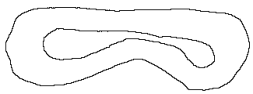
\includegraphics[interpolate=true,width=2.530000in,height=0.940000in]{contents/chapt7/figs/model/cornering_stiffness-img0.png}}%
\end{pgfscope}%
\begin{pgfscope}%
\pgfpathrectangle{\pgfqpoint{0.150000in}{0.508846in}}{\pgfqpoint{2.525000in}{0.932308in}}%
\pgfusepath{clip}%
\pgfsetrectcap%
\pgfsetroundjoin%
\pgfsetlinewidth{1.505625pt}%
\definecolor{currentstroke}{rgb}{0.121569,0.466667,0.705882}%
\pgfsetstrokecolor{currentstroke}%
\pgfsetstrokeopacity{0.700000}%
\pgfsetdash{}{0pt}%
\pgfpathmoveto{\pgfqpoint{1.703846in}{1.208077in}}%
\pgfpathlineto{\pgfqpoint{1.638816in}{1.209065in}}%
\pgfpathlineto{\pgfqpoint{1.576283in}{1.212383in}}%
\pgfpathlineto{\pgfqpoint{1.485221in}{1.219788in}}%
\pgfpathlineto{\pgfqpoint{1.356954in}{1.230720in}}%
\pgfpathlineto{\pgfqpoint{1.294588in}{1.233590in}}%
\pgfpathlineto{\pgfqpoint{1.200947in}{1.234983in}}%
\pgfpathlineto{\pgfqpoint{0.951216in}{1.235676in}}%
\pgfpathlineto{\pgfqpoint{0.888831in}{1.233236in}}%
\pgfpathlineto{\pgfqpoint{0.834359in}{1.229120in}}%
\pgfpathlineto{\pgfqpoint{0.780088in}{1.222885in}}%
\pgfpathlineto{\pgfqpoint{0.726121in}{1.214419in}}%
\pgfpathlineto{\pgfqpoint{0.672559in}{1.203686in}}%
\pgfpathlineto{\pgfqpoint{0.634793in}{1.193896in}}%
\pgfpathlineto{\pgfqpoint{0.605284in}{1.183733in}}%
\pgfpathlineto{\pgfqpoint{0.583817in}{1.174401in}}%
\pgfpathlineto{\pgfqpoint{0.563166in}{1.163382in}}%
\pgfpathlineto{\pgfqpoint{0.543586in}{1.150558in}}%
\pgfpathlineto{\pgfqpoint{0.525405in}{1.135822in}}%
\pgfpathlineto{\pgfqpoint{0.509058in}{1.119078in}}%
\pgfpathlineto{\pgfqpoint{0.494879in}{1.100463in}}%
\pgfpathlineto{\pgfqpoint{0.483231in}{1.080171in}}%
\pgfpathlineto{\pgfqpoint{0.474431in}{1.058492in}}%
\pgfpathlineto{\pgfqpoint{0.468761in}{1.035794in}}%
\pgfpathlineto{\pgfqpoint{0.466812in}{1.020312in}}%
\pgfpathlineto{\pgfqpoint{0.466651in}{0.996915in}}%
\pgfpathlineto{\pgfqpoint{0.469561in}{0.973697in}}%
\pgfpathlineto{\pgfqpoint{0.475243in}{0.950997in}}%
\pgfpathlineto{\pgfqpoint{0.483490in}{0.929095in}}%
\pgfpathlineto{\pgfqpoint{0.494006in}{0.908186in}}%
\pgfpathlineto{\pgfqpoint{0.506529in}{0.888413in}}%
\pgfpathlineto{\pgfqpoint{0.520810in}{0.869868in}}%
\pgfpathlineto{\pgfqpoint{0.536555in}{0.852546in}}%
\pgfpathlineto{\pgfqpoint{0.553547in}{0.836445in}}%
\pgfpathlineto{\pgfqpoint{0.577876in}{0.816900in}}%
\pgfpathlineto{\pgfqpoint{0.603800in}{0.799522in}}%
\pgfpathlineto{\pgfqpoint{0.631038in}{0.784285in}}%
\pgfpathlineto{\pgfqpoint{0.659377in}{0.771209in}}%
\pgfpathlineto{\pgfqpoint{0.688718in}{0.760574in}}%
\pgfpathlineto{\pgfqpoint{0.718877in}{0.752551in}}%
\pgfpathlineto{\pgfqpoint{0.749646in}{0.747343in}}%
\pgfpathlineto{\pgfqpoint{0.772974in}{0.745398in}}%
\pgfpathlineto{\pgfqpoint{0.796381in}{0.745187in}}%
\pgfpathlineto{\pgfqpoint{0.827513in}{0.747385in}}%
\pgfpathlineto{\pgfqpoint{0.858355in}{0.752162in}}%
\pgfpathlineto{\pgfqpoint{0.888737in}{0.759306in}}%
\pgfpathlineto{\pgfqpoint{0.918546in}{0.768560in}}%
\pgfpathlineto{\pgfqpoint{0.947696in}{0.779718in}}%
\pgfpathlineto{\pgfqpoint{0.983229in}{0.795837in}}%
\pgfpathlineto{\pgfqpoint{1.060017in}{0.834222in}}%
\pgfpathlineto{\pgfqpoint{1.109380in}{0.857621in}}%
\pgfpathlineto{\pgfqpoint{1.159684in}{0.878918in}}%
\pgfpathlineto{\pgfqpoint{1.210910in}{0.897891in}}%
\pgfpathlineto{\pgfqpoint{1.262928in}{0.914570in}}%
\pgfpathlineto{\pgfqpoint{1.315613in}{0.929003in}}%
\pgfpathlineto{\pgfqpoint{1.368866in}{0.941182in}}%
\pgfpathlineto{\pgfqpoint{1.414853in}{0.949525in}}%
\pgfpathlineto{\pgfqpoint{1.453370in}{0.954179in}}%
\pgfpathlineto{\pgfqpoint{1.484250in}{0.956075in}}%
\pgfpathlineto{\pgfqpoint{1.515100in}{0.956086in}}%
\pgfpathlineto{\pgfqpoint{1.545825in}{0.954075in}}%
\pgfpathlineto{\pgfqpoint{1.584073in}{0.949127in}}%
\pgfpathlineto{\pgfqpoint{1.622056in}{0.941875in}}%
\pgfpathlineto{\pgfqpoint{1.667245in}{0.930758in}}%
\pgfpathlineto{\pgfqpoint{1.711653in}{0.917508in}}%
\pgfpathlineto{\pgfqpoint{1.747302in}{0.904712in}}%
\pgfpathlineto{\pgfqpoint{1.781498in}{0.890120in}}%
\pgfpathlineto{\pgfqpoint{1.813988in}{0.873526in}}%
\pgfpathlineto{\pgfqpoint{1.844501in}{0.854985in}}%
\pgfpathlineto{\pgfqpoint{1.872871in}{0.834830in}}%
\pgfpathlineto{\pgfqpoint{1.899034in}{0.813277in}}%
\pgfpathlineto{\pgfqpoint{1.923017in}{0.790618in}}%
\pgfpathlineto{\pgfqpoint{1.949971in}{0.761659in}}%
\pgfpathlineto{\pgfqpoint{1.987425in}{0.721323in}}%
\pgfpathlineto{\pgfqpoint{2.013420in}{0.696805in}}%
\pgfpathlineto{\pgfqpoint{2.036131in}{0.678185in}}%
\pgfpathlineto{\pgfqpoint{2.060941in}{0.660906in}}%
\pgfpathlineto{\pgfqpoint{2.081042in}{0.649208in}}%
\pgfpathlineto{\pgfqpoint{2.102128in}{0.639009in}}%
\pgfpathlineto{\pgfqpoint{2.123997in}{0.630625in}}%
\pgfpathlineto{\pgfqpoint{2.146562in}{0.624356in}}%
\pgfpathlineto{\pgfqpoint{2.169613in}{0.620460in}}%
\pgfpathlineto{\pgfqpoint{2.192633in}{0.619086in}}%
\pgfpathlineto{\pgfqpoint{2.215297in}{0.620406in}}%
\pgfpathlineto{\pgfqpoint{2.237259in}{0.624515in}}%
\pgfpathlineto{\pgfqpoint{2.258126in}{0.631438in}}%
\pgfpathlineto{\pgfqpoint{2.277497in}{0.641057in}}%
\pgfpathlineto{\pgfqpoint{2.294979in}{0.653174in}}%
\pgfpathlineto{\pgfqpoint{2.310249in}{0.667492in}}%
\pgfpathlineto{\pgfqpoint{2.323190in}{0.683568in}}%
\pgfpathlineto{\pgfqpoint{2.333911in}{0.700856in}}%
\pgfpathlineto{\pgfqpoint{2.342694in}{0.718876in}}%
\pgfpathlineto{\pgfqpoint{2.352107in}{0.743396in}}%
\pgfpathlineto{\pgfqpoint{2.361274in}{0.774145in}}%
\pgfpathlineto{\pgfqpoint{2.371828in}{0.818495in}}%
\pgfpathlineto{\pgfqpoint{2.377716in}{0.851750in}}%
\pgfpathlineto{\pgfqpoint{2.381558in}{0.886317in}}%
\pgfpathlineto{\pgfqpoint{2.382727in}{0.914835in}}%
\pgfpathlineto{\pgfqpoint{2.381734in}{0.943888in}}%
\pgfpathlineto{\pgfqpoint{2.379060in}{0.965862in}}%
\pgfpathlineto{\pgfqpoint{2.374424in}{0.987798in}}%
\pgfpathlineto{\pgfqpoint{2.367641in}{1.009464in}}%
\pgfpathlineto{\pgfqpoint{2.358568in}{1.030585in}}%
\pgfpathlineto{\pgfqpoint{2.347113in}{1.050841in}}%
\pgfpathlineto{\pgfqpoint{2.333440in}{1.069790in}}%
\pgfpathlineto{\pgfqpoint{2.317865in}{1.087210in}}%
\pgfpathlineto{\pgfqpoint{2.300634in}{1.102994in}}%
\pgfpathlineto{\pgfqpoint{2.281915in}{1.116983in}}%
\pgfpathlineto{\pgfqpoint{2.261945in}{1.129120in}}%
\pgfpathlineto{\pgfqpoint{2.240947in}{1.139377in}}%
\pgfpathlineto{\pgfqpoint{2.219134in}{1.147766in}}%
\pgfpathlineto{\pgfqpoint{2.189177in}{1.156337in}}%
\pgfpathlineto{\pgfqpoint{2.158602in}{1.162352in}}%
\pgfpathlineto{\pgfqpoint{2.127666in}{1.166110in}}%
\pgfpathlineto{\pgfqpoint{2.088766in}{1.168141in}}%
\pgfpathlineto{\pgfqpoint{2.049811in}{1.167742in}}%
\pgfpathlineto{\pgfqpoint{1.925207in}{1.164132in}}%
\pgfpathlineto{\pgfqpoint{1.886282in}{1.165722in}}%
\pgfpathlineto{\pgfqpoint{1.839704in}{1.169722in}}%
\pgfpathlineto{\pgfqpoint{1.785610in}{1.176696in}}%
\pgfpathlineto{\pgfqpoint{1.770199in}{1.179019in}}%
\pgfpathlineto{\pgfqpoint{1.770199in}{1.179019in}}%
\pgfusepath{stroke}%
\end{pgfscope}%
\begin{pgfscope}%
\pgfpathrectangle{\pgfqpoint{0.150000in}{0.508846in}}{\pgfqpoint{2.525000in}{0.932308in}}%
\pgfusepath{clip}%
\pgfsetrectcap%
\pgfsetroundjoin%
\pgfsetlinewidth{1.505625pt}%
\definecolor{currentstroke}{rgb}{1.000000,0.498039,0.054902}%
\pgfsetstrokecolor{currentstroke}%
\pgfsetstrokeopacity{0.700000}%
\pgfsetdash{}{0pt}%
\pgfpathmoveto{\pgfqpoint{1.703846in}{1.208077in}}%
\pgfpathlineto{\pgfqpoint{1.638673in}{1.209160in}}%
\pgfpathlineto{\pgfqpoint{1.581829in}{1.212338in}}%
\pgfpathlineto{\pgfqpoint{1.498158in}{1.219520in}}%
\pgfpathlineto{\pgfqpoint{1.339628in}{1.233961in}}%
\pgfpathlineto{\pgfqpoint{1.284690in}{1.236272in}}%
\pgfpathlineto{\pgfqpoint{1.127666in}{1.241158in}}%
\pgfpathlineto{\pgfqpoint{0.986474in}{1.248696in}}%
\pgfpathlineto{\pgfqpoint{0.939344in}{1.248834in}}%
\pgfpathlineto{\pgfqpoint{0.892270in}{1.246591in}}%
\pgfpathlineto{\pgfqpoint{0.853203in}{1.242566in}}%
\pgfpathlineto{\pgfqpoint{0.814400in}{1.236498in}}%
\pgfpathlineto{\pgfqpoint{0.768222in}{1.227073in}}%
\pgfpathlineto{\pgfqpoint{0.714876in}{1.213747in}}%
\pgfpathlineto{\pgfqpoint{0.654494in}{1.196337in}}%
\pgfpathlineto{\pgfqpoint{0.617394in}{1.183461in}}%
\pgfpathlineto{\pgfqpoint{0.588641in}{1.170811in}}%
\pgfpathlineto{\pgfqpoint{0.567950in}{1.159541in}}%
\pgfpathlineto{\pgfqpoint{0.548336in}{1.146490in}}%
\pgfpathlineto{\pgfqpoint{0.530155in}{1.131513in}}%
\pgfpathlineto{\pgfqpoint{0.513948in}{1.114424in}}%
\pgfpathlineto{\pgfqpoint{0.500189in}{1.095311in}}%
\pgfpathlineto{\pgfqpoint{0.492599in}{1.081561in}}%
\pgfpathlineto{\pgfqpoint{0.486430in}{1.067117in}}%
\pgfpathlineto{\pgfqpoint{0.481804in}{1.052109in}}%
\pgfpathlineto{\pgfqpoint{0.478821in}{1.036689in}}%
\pgfpathlineto{\pgfqpoint{0.477558in}{1.021035in}}%
\pgfpathlineto{\pgfqpoint{0.478064in}{1.005339in}}%
\pgfpathlineto{\pgfqpoint{0.480334in}{0.989798in}}%
\pgfpathlineto{\pgfqpoint{0.484258in}{0.974591in}}%
\pgfpathlineto{\pgfqpoint{0.489710in}{0.959861in}}%
\pgfpathlineto{\pgfqpoint{0.500440in}{0.938898in}}%
\pgfpathlineto{\pgfqpoint{0.513892in}{0.919565in}}%
\pgfpathlineto{\pgfqpoint{0.529654in}{0.902062in}}%
\pgfpathlineto{\pgfqpoint{0.547306in}{0.886463in}}%
\pgfpathlineto{\pgfqpoint{0.566504in}{0.872810in}}%
\pgfpathlineto{\pgfqpoint{0.586907in}{0.861027in}}%
\pgfpathlineto{\pgfqpoint{0.615383in}{0.847769in}}%
\pgfpathlineto{\pgfqpoint{0.644900in}{0.837013in}}%
\pgfpathlineto{\pgfqpoint{0.675102in}{0.828359in}}%
\pgfpathlineto{\pgfqpoint{0.713461in}{0.819938in}}%
\pgfpathlineto{\pgfqpoint{0.752293in}{0.814084in}}%
\pgfpathlineto{\pgfqpoint{0.791432in}{0.810872in}}%
\pgfpathlineto{\pgfqpoint{0.822845in}{0.810313in}}%
\pgfpathlineto{\pgfqpoint{0.854233in}{0.811661in}}%
\pgfpathlineto{\pgfqpoint{0.885477in}{0.814962in}}%
\pgfpathlineto{\pgfqpoint{0.924211in}{0.821441in}}%
\pgfpathlineto{\pgfqpoint{0.962472in}{0.830295in}}%
\pgfpathlineto{\pgfqpoint{1.000213in}{0.841162in}}%
\pgfpathlineto{\pgfqpoint{1.044810in}{0.856405in}}%
\pgfpathlineto{\pgfqpoint{1.155915in}{0.895624in}}%
\pgfpathlineto{\pgfqpoint{1.208733in}{0.910908in}}%
\pgfpathlineto{\pgfqpoint{1.262153in}{0.923938in}}%
\pgfpathlineto{\pgfqpoint{1.323697in}{0.936647in}}%
\pgfpathlineto{\pgfqpoint{1.377917in}{0.945785in}}%
\pgfpathlineto{\pgfqpoint{1.424704in}{0.951451in}}%
\pgfpathlineto{\pgfqpoint{1.463880in}{0.954233in}}%
\pgfpathlineto{\pgfqpoint{1.503146in}{0.954972in}}%
\pgfpathlineto{\pgfqpoint{1.542393in}{0.953530in}}%
\pgfpathlineto{\pgfqpoint{1.581488in}{0.949809in}}%
\pgfpathlineto{\pgfqpoint{1.620297in}{0.943788in}}%
\pgfpathlineto{\pgfqpoint{1.658526in}{0.935479in}}%
\pgfpathlineto{\pgfqpoint{1.695810in}{0.924942in}}%
\pgfpathlineto{\pgfqpoint{1.731985in}{0.912155in}}%
\pgfpathlineto{\pgfqpoint{1.766895in}{0.897169in}}%
\pgfpathlineto{\pgfqpoint{1.800348in}{0.880194in}}%
\pgfpathlineto{\pgfqpoint{1.832200in}{0.861608in}}%
\pgfpathlineto{\pgfqpoint{1.862442in}{0.841631in}}%
\pgfpathlineto{\pgfqpoint{1.896642in}{0.816140in}}%
\pgfpathlineto{\pgfqpoint{2.001708in}{0.732833in}}%
\pgfpathlineto{\pgfqpoint{2.027771in}{0.715863in}}%
\pgfpathlineto{\pgfqpoint{2.054902in}{0.700664in}}%
\pgfpathlineto{\pgfqpoint{2.083125in}{0.687610in}}%
\pgfpathlineto{\pgfqpoint{2.112369in}{0.677041in}}%
\pgfpathlineto{\pgfqpoint{2.142467in}{0.669240in}}%
\pgfpathlineto{\pgfqpoint{2.165462in}{0.665339in}}%
\pgfpathlineto{\pgfqpoint{2.188699in}{0.663359in}}%
\pgfpathlineto{\pgfqpoint{2.212019in}{0.663507in}}%
\pgfpathlineto{\pgfqpoint{2.235217in}{0.665890in}}%
\pgfpathlineto{\pgfqpoint{2.258054in}{0.670606in}}%
\pgfpathlineto{\pgfqpoint{2.280254in}{0.677739in}}%
\pgfpathlineto{\pgfqpoint{2.301527in}{0.687287in}}%
\pgfpathlineto{\pgfqpoint{2.321580in}{0.699186in}}%
\pgfpathlineto{\pgfqpoint{2.340173in}{0.713257in}}%
\pgfpathlineto{\pgfqpoint{2.357066in}{0.729330in}}%
\pgfpathlineto{\pgfqpoint{2.372039in}{0.747204in}}%
\pgfpathlineto{\pgfqpoint{2.384932in}{0.766633in}}%
\pgfpathlineto{\pgfqpoint{2.395590in}{0.787373in}}%
\pgfpathlineto{\pgfqpoint{2.403910in}{0.809156in}}%
\pgfpathlineto{\pgfqpoint{2.409816in}{0.831714in}}%
\pgfpathlineto{\pgfqpoint{2.413336in}{0.854766in}}%
\pgfpathlineto{\pgfqpoint{2.414466in}{0.878058in}}%
\pgfpathlineto{\pgfqpoint{2.413222in}{0.901344in}}%
\pgfpathlineto{\pgfqpoint{2.409677in}{0.924393in}}%
\pgfpathlineto{\pgfqpoint{2.403884in}{0.946982in}}%
\pgfpathlineto{\pgfqpoint{2.395940in}{0.968907in}}%
\pgfpathlineto{\pgfqpoint{2.386022in}{0.990014in}}%
\pgfpathlineto{\pgfqpoint{2.374236in}{1.010139in}}%
\pgfpathlineto{\pgfqpoint{2.360729in}{1.029151in}}%
\pgfpathlineto{\pgfqpoint{2.345631in}{1.046926in}}%
\pgfpathlineto{\pgfqpoint{2.329093in}{1.063371in}}%
\pgfpathlineto{\pgfqpoint{2.311245in}{1.078382in}}%
\pgfpathlineto{\pgfqpoint{2.292231in}{1.091889in}}%
\pgfpathlineto{\pgfqpoint{2.265467in}{1.107720in}}%
\pgfpathlineto{\pgfqpoint{2.237520in}{1.121360in}}%
\pgfpathlineto{\pgfqpoint{2.208692in}{1.133026in}}%
\pgfpathlineto{\pgfqpoint{2.171804in}{1.145293in}}%
\pgfpathlineto{\pgfqpoint{2.134249in}{1.155338in}}%
\pgfpathlineto{\pgfqpoint{2.096184in}{1.163234in}}%
\pgfpathlineto{\pgfqpoint{2.057736in}{1.168987in}}%
\pgfpathlineto{\pgfqpoint{2.019024in}{1.172546in}}%
\pgfpathlineto{\pgfqpoint{1.972400in}{1.174172in}}%
\pgfpathlineto{\pgfqpoint{1.840265in}{1.177360in}}%
\pgfpathlineto{\pgfqpoint{1.793793in}{1.181465in}}%
\pgfpathlineto{\pgfqpoint{1.747567in}{1.187758in}}%
\pgfpathlineto{\pgfqpoint{1.709303in}{1.194641in}}%
\pgfpathlineto{\pgfqpoint{1.709303in}{1.194641in}}%
\pgfusepath{stroke}%
\end{pgfscope}%
\begin{pgfscope}%
\definecolor{textcolor}{rgb}{0.000000,0.000000,0.000000}%
\pgfsetstrokecolor{textcolor}%
\pgfsetfillcolor{textcolor}%
\pgftext[x=1.412500in,y=1.524487in,,base]{\color{textcolor}\rmfamily\fontsize{12.000000}{14.400000}\selectfont End-to-end}%
\end{pgfscope}%
\begin{pgfscope}%
\pgfpathrectangle{\pgfqpoint{2.825000in}{0.508846in}}{\pgfqpoint{2.525000in}{0.932308in}}%
\pgfusepath{clip}%
\pgfsys@transformshift{2.825000in}{0.508846in}%
\pgftext[left,bottom]{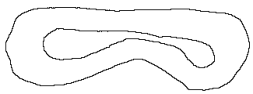
\includegraphics[interpolate=true,width=2.530000in,height=0.940000in]{contents/chapt7/figs/model/cornering_stiffness-img1.png}}%
\end{pgfscope}%
\begin{pgfscope}%
\pgfpathrectangle{\pgfqpoint{2.825000in}{0.508846in}}{\pgfqpoint{2.525000in}{0.932308in}}%
\pgfusepath{clip}%
\pgfsetrectcap%
\pgfsetroundjoin%
\pgfsetlinewidth{1.505625pt}%
\definecolor{currentstroke}{rgb}{0.121569,0.466667,0.705882}%
\pgfsetstrokecolor{currentstroke}%
\pgfsetstrokeopacity{0.700000}%
\pgfsetdash{}{0pt}%
\pgfpathmoveto{\pgfqpoint{4.378846in}{1.208077in}}%
\pgfpathlineto{\pgfqpoint{4.319458in}{1.209146in}}%
\pgfpathlineto{\pgfqpoint{4.272471in}{1.212520in}}%
\pgfpathlineto{\pgfqpoint{4.227084in}{1.217894in}}%
\pgfpathlineto{\pgfqpoint{4.103399in}{1.234024in}}%
\pgfpathlineto{\pgfqpoint{4.056752in}{1.237459in}}%
\pgfpathlineto{\pgfqpoint{4.009985in}{1.238234in}}%
\pgfpathlineto{\pgfqpoint{3.963238in}{1.236617in}}%
\pgfpathlineto{\pgfqpoint{3.807564in}{1.228491in}}%
\pgfpathlineto{\pgfqpoint{3.768613in}{1.229921in}}%
\pgfpathlineto{\pgfqpoint{3.706456in}{1.235074in}}%
\pgfpathlineto{\pgfqpoint{3.644273in}{1.239878in}}%
\pgfpathlineto{\pgfqpoint{3.597516in}{1.241143in}}%
\pgfpathlineto{\pgfqpoint{3.550758in}{1.239981in}}%
\pgfpathlineto{\pgfqpoint{3.504144in}{1.236127in}}%
\pgfpathlineto{\pgfqpoint{3.457827in}{1.229611in}}%
\pgfpathlineto{\pgfqpoint{3.404246in}{1.219267in}}%
\pgfpathlineto{\pgfqpoint{3.351219in}{1.206380in}}%
\pgfpathlineto{\pgfqpoint{3.313826in}{1.195374in}}%
\pgfpathlineto{\pgfqpoint{3.277104in}{1.182312in}}%
\pgfpathlineto{\pgfqpoint{3.248495in}{1.169915in}}%
\pgfpathlineto{\pgfqpoint{3.220980in}{1.155257in}}%
\pgfpathlineto{\pgfqpoint{3.201361in}{1.142532in}}%
\pgfpathlineto{\pgfqpoint{3.182918in}{1.128160in}}%
\pgfpathlineto{\pgfqpoint{3.165930in}{1.112094in}}%
\pgfpathlineto{\pgfqpoint{3.150665in}{1.094386in}}%
\pgfpathlineto{\pgfqpoint{3.137445in}{1.075104in}}%
\pgfpathlineto{\pgfqpoint{3.126537in}{1.054428in}}%
\pgfpathlineto{\pgfqpoint{3.118241in}{1.032574in}}%
\pgfpathlineto{\pgfqpoint{3.112770in}{1.009848in}}%
\pgfpathlineto{\pgfqpoint{3.110226in}{0.986611in}}%
\pgfpathlineto{\pgfqpoint{3.110584in}{0.963237in}}%
\pgfpathlineto{\pgfqpoint{3.113647in}{0.940060in}}%
\pgfpathlineto{\pgfqpoint{3.119320in}{0.917380in}}%
\pgfpathlineto{\pgfqpoint{3.127436in}{0.895456in}}%
\pgfpathlineto{\pgfqpoint{3.137889in}{0.874543in}}%
\pgfpathlineto{\pgfqpoint{3.150571in}{0.854904in}}%
\pgfpathlineto{\pgfqpoint{3.165373in}{0.836808in}}%
\pgfpathlineto{\pgfqpoint{3.182040in}{0.820412in}}%
\pgfpathlineto{\pgfqpoint{3.200364in}{0.805893in}}%
\pgfpathlineto{\pgfqpoint{3.220148in}{0.793435in}}%
\pgfpathlineto{\pgfqpoint{3.241145in}{0.783152in}}%
\pgfpathlineto{\pgfqpoint{3.263105in}{0.775126in}}%
\pgfpathlineto{\pgfqpoint{3.285755in}{0.769320in}}%
\pgfpathlineto{\pgfqpoint{3.308849in}{0.765657in}}%
\pgfpathlineto{\pgfqpoint{3.332164in}{0.763860in}}%
\pgfpathlineto{\pgfqpoint{3.363342in}{0.763925in}}%
\pgfpathlineto{\pgfqpoint{3.394430in}{0.766317in}}%
\pgfpathlineto{\pgfqpoint{3.432983in}{0.772036in}}%
\pgfpathlineto{\pgfqpoint{3.471115in}{0.780114in}}%
\pgfpathlineto{\pgfqpoint{3.531552in}{0.795522in}}%
\pgfpathlineto{\pgfqpoint{3.644736in}{0.824902in}}%
\pgfpathlineto{\pgfqpoint{3.682998in}{0.832342in}}%
\pgfpathlineto{\pgfqpoint{3.721600in}{0.837746in}}%
\pgfpathlineto{\pgfqpoint{3.768213in}{0.841619in}}%
\pgfpathlineto{\pgfqpoint{3.916000in}{0.851400in}}%
\pgfpathlineto{\pgfqpoint{3.977885in}{0.859157in}}%
\pgfpathlineto{\pgfqpoint{4.124660in}{0.879042in}}%
\pgfpathlineto{\pgfqpoint{4.163547in}{0.881694in}}%
\pgfpathlineto{\pgfqpoint{4.202521in}{0.882006in}}%
\pgfpathlineto{\pgfqpoint{4.233652in}{0.880228in}}%
\pgfpathlineto{\pgfqpoint{4.264585in}{0.876316in}}%
\pgfpathlineto{\pgfqpoint{4.295159in}{0.870202in}}%
\pgfpathlineto{\pgfqpoint{4.325250in}{0.862030in}}%
\pgfpathlineto{\pgfqpoint{4.354774in}{0.851999in}}%
\pgfpathlineto{\pgfqpoint{4.390911in}{0.837389in}}%
\pgfpathlineto{\pgfqpoint{4.483490in}{0.796138in}}%
\pgfpathlineto{\pgfqpoint{4.661935in}{0.717831in}}%
\pgfpathlineto{\pgfqpoint{4.712002in}{0.697576in}}%
\pgfpathlineto{\pgfqpoint{4.748264in}{0.685655in}}%
\pgfpathlineto{\pgfqpoint{4.777755in}{0.678723in}}%
\pgfpathlineto{\pgfqpoint{4.800122in}{0.675594in}}%
\pgfpathlineto{\pgfqpoint{4.822584in}{0.674438in}}%
\pgfpathlineto{\pgfqpoint{4.844964in}{0.675399in}}%
\pgfpathlineto{\pgfqpoint{4.867043in}{0.678600in}}%
\pgfpathlineto{\pgfqpoint{4.888598in}{0.684000in}}%
\pgfpathlineto{\pgfqpoint{4.909417in}{0.691507in}}%
\pgfpathlineto{\pgfqpoint{4.929293in}{0.701035in}}%
\pgfpathlineto{\pgfqpoint{4.948351in}{0.712555in}}%
\pgfpathlineto{\pgfqpoint{4.967128in}{0.726060in}}%
\pgfpathlineto{\pgfqpoint{4.990938in}{0.746245in}}%
\pgfpathlineto{\pgfqpoint{5.012828in}{0.768499in}}%
\pgfpathlineto{\pgfqpoint{5.027767in}{0.786528in}}%
\pgfpathlineto{\pgfqpoint{5.041241in}{0.805676in}}%
\pgfpathlineto{\pgfqpoint{5.053051in}{0.825892in}}%
\pgfpathlineto{\pgfqpoint{5.063160in}{0.847010in}}%
\pgfpathlineto{\pgfqpoint{5.071442in}{0.868909in}}%
\pgfpathlineto{\pgfqpoint{5.077755in}{0.891454in}}%
\pgfpathlineto{\pgfqpoint{5.081971in}{0.914483in}}%
\pgfpathlineto{\pgfqpoint{5.084015in}{0.937804in}}%
\pgfpathlineto{\pgfqpoint{5.083654in}{0.961211in}}%
\pgfpathlineto{\pgfqpoint{5.080892in}{0.984458in}}%
\pgfpathlineto{\pgfqpoint{5.075867in}{1.007323in}}%
\pgfpathlineto{\pgfqpoint{5.068580in}{1.029571in}}%
\pgfpathlineto{\pgfqpoint{5.059045in}{1.050951in}}%
\pgfpathlineto{\pgfqpoint{5.047368in}{1.071240in}}%
\pgfpathlineto{\pgfqpoint{5.033619in}{1.090186in}}%
\pgfpathlineto{\pgfqpoint{5.017930in}{1.107560in}}%
\pgfpathlineto{\pgfqpoint{5.000511in}{1.123201in}}%
\pgfpathlineto{\pgfqpoint{4.981659in}{1.137081in}}%
\pgfpathlineto{\pgfqpoint{4.961608in}{1.149169in}}%
\pgfpathlineto{\pgfqpoint{4.940570in}{1.159442in}}%
\pgfpathlineto{\pgfqpoint{4.918771in}{1.167988in}}%
\pgfpathlineto{\pgfqpoint{4.888871in}{1.176957in}}%
\pgfpathlineto{\pgfqpoint{4.858387in}{1.183704in}}%
\pgfpathlineto{\pgfqpoint{4.819897in}{1.190161in}}%
\pgfpathlineto{\pgfqpoint{4.765681in}{1.196973in}}%
\pgfpathlineto{\pgfqpoint{4.695744in}{1.203645in}}%
\pgfpathlineto{\pgfqpoint{4.617870in}{1.209043in}}%
\pgfpathlineto{\pgfqpoint{4.555461in}{1.211271in}}%
\pgfpathlineto{\pgfqpoint{4.493013in}{1.211267in}}%
\pgfpathlineto{\pgfqpoint{4.430583in}{1.209681in}}%
\pgfpathlineto{\pgfqpoint{4.430583in}{1.209681in}}%
\pgfusepath{stroke}%
\end{pgfscope}%
\begin{pgfscope}%
\pgfpathrectangle{\pgfqpoint{2.825000in}{0.508846in}}{\pgfqpoint{2.525000in}{0.932308in}}%
\pgfusepath{clip}%
\pgfsetrectcap%
\pgfsetroundjoin%
\pgfsetlinewidth{1.505625pt}%
\definecolor{currentstroke}{rgb}{1.000000,0.498039,0.054902}%
\pgfsetstrokecolor{currentstroke}%
\pgfsetstrokeopacity{0.700000}%
\pgfsetdash{}{0pt}%
\pgfpathmoveto{\pgfqpoint{4.378846in}{1.208077in}}%
\pgfpathlineto{\pgfqpoint{4.325597in}{1.209062in}}%
\pgfpathlineto{\pgfqpoint{4.286669in}{1.212118in}}%
\pgfpathlineto{\pgfqpoint{4.242734in}{1.217832in}}%
\pgfpathlineto{\pgfqpoint{4.088808in}{1.241428in}}%
\pgfpathlineto{\pgfqpoint{4.042200in}{1.244734in}}%
\pgfpathlineto{\pgfqpoint{3.995489in}{1.245910in}}%
\pgfpathlineto{\pgfqpoint{3.933194in}{1.244988in}}%
\pgfpathlineto{\pgfqpoint{3.808621in}{1.242180in}}%
\pgfpathlineto{\pgfqpoint{3.746333in}{1.243514in}}%
\pgfpathlineto{\pgfqpoint{3.652898in}{1.245449in}}%
\pgfpathlineto{\pgfqpoint{3.606181in}{1.244540in}}%
\pgfpathlineto{\pgfqpoint{3.559566in}{1.241361in}}%
\pgfpathlineto{\pgfqpoint{3.513169in}{1.235835in}}%
\pgfpathlineto{\pgfqpoint{3.467113in}{1.227965in}}%
\pgfpathlineto{\pgfqpoint{3.421483in}{1.217905in}}%
\pgfpathlineto{\pgfqpoint{3.368805in}{1.203882in}}%
\pgfpathlineto{\pgfqpoint{3.324230in}{1.189870in}}%
\pgfpathlineto{\pgfqpoint{3.280439in}{1.173580in}}%
\pgfpathlineto{\pgfqpoint{3.252016in}{1.160842in}}%
\pgfpathlineto{\pgfqpoint{3.224670in}{1.145939in}}%
\pgfpathlineto{\pgfqpoint{3.205194in}{1.133043in}}%
\pgfpathlineto{\pgfqpoint{3.186939in}{1.118473in}}%
\pgfpathlineto{\pgfqpoint{3.170268in}{1.102115in}}%
\pgfpathlineto{\pgfqpoint{3.155522in}{1.084008in}}%
\pgfpathlineto{\pgfqpoint{3.143104in}{1.064232in}}%
\pgfpathlineto{\pgfqpoint{3.133339in}{1.043023in}}%
\pgfpathlineto{\pgfqpoint{3.126434in}{1.020718in}}%
\pgfpathlineto{\pgfqpoint{3.122600in}{0.997687in}}%
\pgfpathlineto{\pgfqpoint{3.121883in}{0.974348in}}%
\pgfpathlineto{\pgfqpoint{3.124167in}{0.951108in}}%
\pgfpathlineto{\pgfqpoint{3.129156in}{0.928295in}}%
\pgfpathlineto{\pgfqpoint{3.136693in}{0.906190in}}%
\pgfpathlineto{\pgfqpoint{3.146624in}{0.885052in}}%
\pgfpathlineto{\pgfqpoint{3.158800in}{0.865123in}}%
\pgfpathlineto{\pgfqpoint{3.173098in}{0.846657in}}%
\pgfpathlineto{\pgfqpoint{3.189396in}{0.829930in}}%
\pgfpathlineto{\pgfqpoint{3.207470in}{0.815141in}}%
\pgfpathlineto{\pgfqpoint{3.227126in}{0.802531in}}%
\pgfpathlineto{\pgfqpoint{3.248119in}{0.792300in}}%
\pgfpathlineto{\pgfqpoint{3.270137in}{0.784513in}}%
\pgfpathlineto{\pgfqpoint{3.292854in}{0.779087in}}%
\pgfpathlineto{\pgfqpoint{3.315992in}{0.775895in}}%
\pgfpathlineto{\pgfqpoint{3.339322in}{0.774738in}}%
\pgfpathlineto{\pgfqpoint{3.370455in}{0.775630in}}%
\pgfpathlineto{\pgfqpoint{3.409207in}{0.779414in}}%
\pgfpathlineto{\pgfqpoint{3.470871in}{0.788318in}}%
\pgfpathlineto{\pgfqpoint{3.547678in}{0.801197in}}%
\pgfpathlineto{\pgfqpoint{3.624106in}{0.816165in}}%
\pgfpathlineto{\pgfqpoint{3.700517in}{0.831204in}}%
\pgfpathlineto{\pgfqpoint{3.746756in}{0.837924in}}%
\pgfpathlineto{\pgfqpoint{3.793259in}{0.842485in}}%
\pgfpathlineto{\pgfqpoint{3.925157in}{0.853826in}}%
\pgfpathlineto{\pgfqpoint{3.986840in}{0.862589in}}%
\pgfpathlineto{\pgfqpoint{4.102330in}{0.880123in}}%
\pgfpathlineto{\pgfqpoint{4.148847in}{0.884507in}}%
\pgfpathlineto{\pgfqpoint{4.187762in}{0.885711in}}%
\pgfpathlineto{\pgfqpoint{4.218891in}{0.884621in}}%
\pgfpathlineto{\pgfqpoint{4.249887in}{0.881549in}}%
\pgfpathlineto{\pgfqpoint{4.280634in}{0.876571in}}%
\pgfpathlineto{\pgfqpoint{4.311020in}{0.869719in}}%
\pgfpathlineto{\pgfqpoint{4.348399in}{0.858822in}}%
\pgfpathlineto{\pgfqpoint{4.385051in}{0.845685in}}%
\pgfpathlineto{\pgfqpoint{4.428044in}{0.827385in}}%
\pgfpathlineto{\pgfqpoint{4.484321in}{0.800656in}}%
\pgfpathlineto{\pgfqpoint{4.560653in}{0.761767in}}%
\pgfpathlineto{\pgfqpoint{4.637123in}{0.723151in}}%
\pgfpathlineto{\pgfqpoint{4.679798in}{0.704161in}}%
\pgfpathlineto{\pgfqpoint{4.708796in}{0.693291in}}%
\pgfpathlineto{\pgfqpoint{4.738302in}{0.684595in}}%
\pgfpathlineto{\pgfqpoint{4.760742in}{0.679846in}}%
\pgfpathlineto{\pgfqpoint{4.783372in}{0.676904in}}%
\pgfpathlineto{\pgfqpoint{4.806059in}{0.676054in}}%
\pgfpathlineto{\pgfqpoint{4.828717in}{0.677418in}}%
\pgfpathlineto{\pgfqpoint{4.851823in}{0.681049in}}%
\pgfpathlineto{\pgfqpoint{4.874639in}{0.686633in}}%
\pgfpathlineto{\pgfqpoint{4.896906in}{0.694114in}}%
\pgfpathlineto{\pgfqpoint{4.918473in}{0.703422in}}%
\pgfpathlineto{\pgfqpoint{4.939168in}{0.714533in}}%
\pgfpathlineto{\pgfqpoint{4.958823in}{0.727394in}}%
\pgfpathlineto{\pgfqpoint{4.977273in}{0.741932in}}%
\pgfpathlineto{\pgfqpoint{4.994463in}{0.757940in}}%
\pgfpathlineto{\pgfqpoint{5.010224in}{0.775356in}}%
\pgfpathlineto{\pgfqpoint{5.024460in}{0.794040in}}%
\pgfpathlineto{\pgfqpoint{5.037017in}{0.813891in}}%
\pgfpathlineto{\pgfqpoint{5.047804in}{0.834757in}}%
\pgfpathlineto{\pgfqpoint{5.056708in}{0.856493in}}%
\pgfpathlineto{\pgfqpoint{5.063614in}{0.878942in}}%
\pgfpathlineto{\pgfqpoint{5.068246in}{0.901968in}}%
\pgfpathlineto{\pgfqpoint{5.070506in}{0.925345in}}%
\pgfpathlineto{\pgfqpoint{5.070262in}{0.948829in}}%
\pgfpathlineto{\pgfqpoint{5.067435in}{0.972143in}}%
\pgfpathlineto{\pgfqpoint{5.061967in}{0.994981in}}%
\pgfpathlineto{\pgfqpoint{5.053889in}{1.017021in}}%
\pgfpathlineto{\pgfqpoint{5.043379in}{1.037924in}}%
\pgfpathlineto{\pgfqpoint{5.030552in}{1.057384in}}%
\pgfpathlineto{\pgfqpoint{5.015588in}{1.075137in}}%
\pgfpathlineto{\pgfqpoint{4.998690in}{1.090930in}}%
\pgfpathlineto{\pgfqpoint{4.980149in}{1.104612in}}%
\pgfpathlineto{\pgfqpoint{4.960286in}{1.116119in}}%
\pgfpathlineto{\pgfqpoint{4.939119in}{1.125591in}}%
\pgfpathlineto{\pgfqpoint{4.909679in}{1.135663in}}%
\pgfpathlineto{\pgfqpoint{4.864585in}{1.147740in}}%
\pgfpathlineto{\pgfqpoint{4.804522in}{1.164060in}}%
\pgfpathlineto{\pgfqpoint{4.767664in}{1.176501in}}%
\pgfpathlineto{\pgfqpoint{4.672420in}{1.210484in}}%
\pgfpathlineto{\pgfqpoint{4.642246in}{1.218091in}}%
\pgfpathlineto{\pgfqpoint{4.611612in}{1.223561in}}%
\pgfpathlineto{\pgfqpoint{4.580686in}{1.227031in}}%
\pgfpathlineto{\pgfqpoint{4.541836in}{1.228982in}}%
\pgfpathlineto{\pgfqpoint{4.495155in}{1.228711in}}%
\pgfpathlineto{\pgfqpoint{4.417363in}{1.227487in}}%
\pgfpathlineto{\pgfqpoint{4.378513in}{1.229421in}}%
\pgfpathlineto{\pgfqpoint{4.378513in}{1.229421in}}%
\pgfusepath{stroke}%
\end{pgfscope}%
\begin{pgfscope}%
\definecolor{textcolor}{rgb}{0.000000,0.000000,0.000000}%
\pgfsetstrokecolor{textcolor}%
\pgfsetfillcolor{textcolor}%
\pgftext[x=4.087500in,y=1.524487in,,base]{\color{textcolor}\rmfamily\fontsize{12.000000}{14.400000}\selectfont Steering and velocity controllers}%
\end{pgfscope}%
\begin{pgfscope}%
\pgfsetbuttcap%
\pgfsetmiterjoin%
\definecolor{currentfill}{rgb}{1.000000,1.000000,1.000000}%
\pgfsetfillcolor{currentfill}%
\pgfsetfillopacity{0.800000}%
\pgfsetlinewidth{1.003750pt}%
\definecolor{currentstroke}{rgb}{0.800000,0.800000,0.800000}%
\pgfsetstrokecolor{currentstroke}%
\pgfsetstrokeopacity{0.800000}%
\pgfsetdash{}{0pt}%
\pgfpathmoveto{\pgfqpoint{0.937900in}{0.069444in}}%
\pgfpathlineto{\pgfqpoint{4.562100in}{0.069444in}}%
\pgfpathquadraticcurveto{\pgfqpoint{4.589878in}{0.069444in}}{\pgfqpoint{4.589878in}{0.097222in}}%
\pgfpathlineto{\pgfqpoint{4.589878in}{0.444675in}}%
\pgfpathquadraticcurveto{\pgfqpoint{4.589878in}{0.472452in}}{\pgfqpoint{4.562100in}{0.472452in}}%
\pgfpathlineto{\pgfqpoint{0.937900in}{0.472452in}}%
\pgfpathquadraticcurveto{\pgfqpoint{0.910122in}{0.472452in}}{\pgfqpoint{0.910122in}{0.444675in}}%
\pgfpathlineto{\pgfqpoint{0.910122in}{0.097222in}}%
\pgfpathquadraticcurveto{\pgfqpoint{0.910122in}{0.069444in}}{\pgfqpoint{0.937900in}{0.069444in}}%
\pgfpathlineto{\pgfqpoint{0.937900in}{0.069444in}}%
\pgfpathclose%
\pgfusepath{stroke,fill}%
\end{pgfscope}%
\begin{pgfscope}%
\pgfsetrectcap%
\pgfsetroundjoin%
\pgfsetlinewidth{1.505625pt}%
\definecolor{currentstroke}{rgb}{0.121569,0.466667,0.705882}%
\pgfsetstrokecolor{currentstroke}%
\pgfsetstrokeopacity{0.700000}%
\pgfsetdash{}{0pt}%
\pgfpathmoveto{\pgfqpoint{0.965678in}{0.266798in}}%
\pgfpathlineto{\pgfqpoint{1.104567in}{0.266798in}}%
\pgfpathlineto{\pgfqpoint{1.243456in}{0.266798in}}%
\pgfusepath{stroke}%
\end{pgfscope}%
\begin{pgfscope}%
\definecolor{textcolor}{rgb}{0.000000,0.000000,0.000000}%
\pgfsetstrokecolor{textcolor}%
\pgfsetfillcolor{textcolor}%
\pgftext[x=1.354567in,y=0.218187in,left,base]{\color{textcolor}\rmfamily\fontsize{10.000000}{12.000000}\selectfont No model error}%
\end{pgfscope}%
\begin{pgfscope}%
\pgfsetrectcap%
\pgfsetroundjoin%
\pgfsetlinewidth{1.505625pt}%
\definecolor{currentstroke}{rgb}{1.000000,0.498039,0.054902}%
\pgfsetstrokecolor{currentstroke}%
\pgfsetstrokeopacity{0.700000}%
\pgfsetdash{}{0pt}%
\pgfpathmoveto{\pgfqpoint{2.721619in}{0.266798in}}%
\pgfpathlineto{\pgfqpoint{2.860508in}{0.266798in}}%
\pgfpathlineto{\pgfqpoint{2.999396in}{0.266798in}}%
\pgfusepath{stroke}%
\end{pgfscope}%
\begin{pgfscope}%
\definecolor{textcolor}{rgb}{0.000000,0.000000,0.000000}%
\pgfsetstrokecolor{textcolor}%
\pgfsetfillcolor{textcolor}%
\pgftext[x=3.110507in, y=0.311374in, left, base]{\color{textcolor}\rmfamily\fontsize{10.000000}{12.000000}\selectfont Increased front tire }%
\end{pgfscope}%
\begin{pgfscope}%
\definecolor{textcolor}{rgb}{0.000000,0.000000,0.000000}%
\pgfsetstrokecolor{textcolor}%
\pgfsetfillcolor{textcolor}%
\pgftext[x=3.110507in, y=0.155856in, left, base]{\color{textcolor}\rmfamily\fontsize{10.000000}{12.000000}\selectfont cornering stiffness}%
\end{pgfscope}%
\end{pgfpicture}%
\makeatother%
\endgroup%

    \caption[Success rate under test conditions of agents with mismatched tire cornering stiffness]{Success rate under test conditions of agents with mismatched tire cornering stiffness.}
    \label{fig:c_s}
\end{figure}

\textbf{Front tire cornering stiffness}: 
From Figure \ref{fig:c_s}, we see that end-to-end agents are far more sensitive to a front tire cornering stiffness mismatch than partial end-to-end agents.
Specifically, end-to-end agents tend to crash when the front tire cornering stiffness is higher than expected.
The end-to-end agent behaviour that results in this decreased performance is shown on the left of Figure \ref{fig:front_cornering_stiffness_+_paths}.
From this figure, we see that the end-to-end agent comes closer to the inside of the track when the front tire cornering stiffness is increased.
This is because increasing the front tire cornering stiffness decreases slip angle of the tire for a given lateral force, which results in more aggressive cornering.

However, Figure \ref{fig:c_s} shows that our partial-end-to-end agent with both steering and velocity control is robust to changes in front tire cornering stiffness.
The behaviour of this agent is shown on the right of Figure \ref{fig:front_cornering_stiffness_+_paths}.
We see that the partial end-to-end agent does not deviate significantly from the original path.
In fact, an increase in the font tire cornering stiffness only results in more accurate path tracking.
Since the paths are constrained such that they do not intersect with the track boundary, the vehicle does not crash when there is an increase in front tire stiffness coefficient.

\begin{figure}[htb!]
    \centering
    %% Creator: Matplotlib, PGF backend
%%
%% To include the figure in your LaTeX document, write
%%   \input{<filename>.pgf}
%%
%% Make sure the required packages are loaded in your preamble
%%   \usepackage{pgf}
%%
%% Also ensure that all the required font packages are loaded; for instance,
%% the lmodern package is sometimes necessary when using math font.
%%   \usepackage{lmodern}
%%
%% Figures using additional raster images can only be included by \input if
%% they are in the same directory as the main LaTeX file. For loading figures
%% from other directories you can use the `import` package
%%   \usepackage{import}
%%
%% and then include the figures with
%%   \import{<path to file>}{<filename>.pgf}
%%
%% Matplotlib used the following preamble
%%   \usepackage{fontspec}
%%   \setmainfont{DejaVuSerif.ttf}[Path=\detokenize{/home/andrew/anaconda3/envs/auto_car_env/lib/python3.9/site-packages/matplotlib/mpl-data/fonts/ttf/}]
%%   \setsansfont{DejaVuSans.ttf}[Path=\detokenize{/home/andrew/anaconda3/envs/auto_car_env/lib/python3.9/site-packages/matplotlib/mpl-data/fonts/ttf/}]
%%   \setmonofont{DejaVuSansMono.ttf}[Path=\detokenize{/home/andrew/anaconda3/envs/auto_car_env/lib/python3.9/site-packages/matplotlib/mpl-data/fonts/ttf/}]
%%
\begingroup%
\makeatletter%
\begin{pgfpicture}%
\pgfpathrectangle{\pgfpointorigin}{\pgfqpoint{5.500000in}{2.000000in}}%
\pgfusepath{use as bounding box, clip}%
\begin{pgfscope}%
\pgfsetbuttcap%
\pgfsetmiterjoin%
\definecolor{currentfill}{rgb}{1.000000,1.000000,1.000000}%
\pgfsetfillcolor{currentfill}%
\pgfsetlinewidth{0.000000pt}%
\definecolor{currentstroke}{rgb}{1.000000,1.000000,1.000000}%
\pgfsetstrokecolor{currentstroke}%
\pgfsetdash{}{0pt}%
\pgfpathmoveto{\pgfqpoint{0.000000in}{0.000000in}}%
\pgfpathlineto{\pgfqpoint{5.500000in}{0.000000in}}%
\pgfpathlineto{\pgfqpoint{5.500000in}{2.000000in}}%
\pgfpathlineto{\pgfqpoint{0.000000in}{2.000000in}}%
\pgfpathlineto{\pgfqpoint{0.000000in}{0.000000in}}%
\pgfpathclose%
\pgfusepath{fill}%
\end{pgfscope}%
\begin{pgfscope}%
\pgfpathrectangle{\pgfqpoint{0.150000in}{0.508846in}}{\pgfqpoint{2.525000in}{0.932308in}}%
\pgfusepath{clip}%
\pgfsys@transformshift{0.150000in}{0.508846in}%
\pgftext[left,bottom]{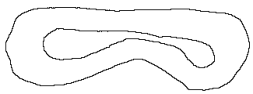
\includegraphics[interpolate=true,width=2.530000in,height=0.940000in]{contents/chapt7/figs/model/cornering_stiffness-img0.png}}%
\end{pgfscope}%
\begin{pgfscope}%
\pgfpathrectangle{\pgfqpoint{0.150000in}{0.508846in}}{\pgfqpoint{2.525000in}{0.932308in}}%
\pgfusepath{clip}%
\pgfsetrectcap%
\pgfsetroundjoin%
\pgfsetlinewidth{1.505625pt}%
\definecolor{currentstroke}{rgb}{0.121569,0.466667,0.705882}%
\pgfsetstrokecolor{currentstroke}%
\pgfsetstrokeopacity{0.700000}%
\pgfsetdash{}{0pt}%
\pgfpathmoveto{\pgfqpoint{1.703846in}{1.208077in}}%
\pgfpathlineto{\pgfqpoint{1.638816in}{1.209065in}}%
\pgfpathlineto{\pgfqpoint{1.576283in}{1.212383in}}%
\pgfpathlineto{\pgfqpoint{1.485221in}{1.219788in}}%
\pgfpathlineto{\pgfqpoint{1.356954in}{1.230720in}}%
\pgfpathlineto{\pgfqpoint{1.294588in}{1.233590in}}%
\pgfpathlineto{\pgfqpoint{1.200947in}{1.234983in}}%
\pgfpathlineto{\pgfqpoint{0.951216in}{1.235676in}}%
\pgfpathlineto{\pgfqpoint{0.888831in}{1.233236in}}%
\pgfpathlineto{\pgfqpoint{0.834359in}{1.229120in}}%
\pgfpathlineto{\pgfqpoint{0.780088in}{1.222885in}}%
\pgfpathlineto{\pgfqpoint{0.726121in}{1.214419in}}%
\pgfpathlineto{\pgfqpoint{0.672559in}{1.203686in}}%
\pgfpathlineto{\pgfqpoint{0.634793in}{1.193896in}}%
\pgfpathlineto{\pgfqpoint{0.605284in}{1.183733in}}%
\pgfpathlineto{\pgfqpoint{0.583817in}{1.174401in}}%
\pgfpathlineto{\pgfqpoint{0.563166in}{1.163382in}}%
\pgfpathlineto{\pgfqpoint{0.543586in}{1.150558in}}%
\pgfpathlineto{\pgfqpoint{0.525405in}{1.135822in}}%
\pgfpathlineto{\pgfqpoint{0.509058in}{1.119078in}}%
\pgfpathlineto{\pgfqpoint{0.494879in}{1.100463in}}%
\pgfpathlineto{\pgfqpoint{0.483231in}{1.080171in}}%
\pgfpathlineto{\pgfqpoint{0.474431in}{1.058492in}}%
\pgfpathlineto{\pgfqpoint{0.468761in}{1.035794in}}%
\pgfpathlineto{\pgfqpoint{0.466812in}{1.020312in}}%
\pgfpathlineto{\pgfqpoint{0.466651in}{0.996915in}}%
\pgfpathlineto{\pgfqpoint{0.469561in}{0.973697in}}%
\pgfpathlineto{\pgfqpoint{0.475243in}{0.950997in}}%
\pgfpathlineto{\pgfqpoint{0.483490in}{0.929095in}}%
\pgfpathlineto{\pgfqpoint{0.494006in}{0.908186in}}%
\pgfpathlineto{\pgfqpoint{0.506529in}{0.888413in}}%
\pgfpathlineto{\pgfqpoint{0.520810in}{0.869868in}}%
\pgfpathlineto{\pgfqpoint{0.536555in}{0.852546in}}%
\pgfpathlineto{\pgfqpoint{0.553547in}{0.836445in}}%
\pgfpathlineto{\pgfqpoint{0.577876in}{0.816900in}}%
\pgfpathlineto{\pgfqpoint{0.603800in}{0.799522in}}%
\pgfpathlineto{\pgfqpoint{0.631038in}{0.784285in}}%
\pgfpathlineto{\pgfqpoint{0.659377in}{0.771209in}}%
\pgfpathlineto{\pgfqpoint{0.688718in}{0.760574in}}%
\pgfpathlineto{\pgfqpoint{0.718877in}{0.752551in}}%
\pgfpathlineto{\pgfqpoint{0.749646in}{0.747343in}}%
\pgfpathlineto{\pgfqpoint{0.772974in}{0.745398in}}%
\pgfpathlineto{\pgfqpoint{0.796381in}{0.745187in}}%
\pgfpathlineto{\pgfqpoint{0.827513in}{0.747385in}}%
\pgfpathlineto{\pgfqpoint{0.858355in}{0.752162in}}%
\pgfpathlineto{\pgfqpoint{0.888737in}{0.759306in}}%
\pgfpathlineto{\pgfqpoint{0.918546in}{0.768560in}}%
\pgfpathlineto{\pgfqpoint{0.947696in}{0.779718in}}%
\pgfpathlineto{\pgfqpoint{0.983229in}{0.795837in}}%
\pgfpathlineto{\pgfqpoint{1.060017in}{0.834222in}}%
\pgfpathlineto{\pgfqpoint{1.109380in}{0.857621in}}%
\pgfpathlineto{\pgfqpoint{1.159684in}{0.878918in}}%
\pgfpathlineto{\pgfqpoint{1.210910in}{0.897891in}}%
\pgfpathlineto{\pgfqpoint{1.262928in}{0.914570in}}%
\pgfpathlineto{\pgfqpoint{1.315613in}{0.929003in}}%
\pgfpathlineto{\pgfqpoint{1.368866in}{0.941182in}}%
\pgfpathlineto{\pgfqpoint{1.414853in}{0.949525in}}%
\pgfpathlineto{\pgfqpoint{1.453370in}{0.954179in}}%
\pgfpathlineto{\pgfqpoint{1.484250in}{0.956075in}}%
\pgfpathlineto{\pgfqpoint{1.515100in}{0.956086in}}%
\pgfpathlineto{\pgfqpoint{1.545825in}{0.954075in}}%
\pgfpathlineto{\pgfqpoint{1.584073in}{0.949127in}}%
\pgfpathlineto{\pgfqpoint{1.622056in}{0.941875in}}%
\pgfpathlineto{\pgfqpoint{1.667245in}{0.930758in}}%
\pgfpathlineto{\pgfqpoint{1.711653in}{0.917508in}}%
\pgfpathlineto{\pgfqpoint{1.747302in}{0.904712in}}%
\pgfpathlineto{\pgfqpoint{1.781498in}{0.890120in}}%
\pgfpathlineto{\pgfqpoint{1.813988in}{0.873526in}}%
\pgfpathlineto{\pgfqpoint{1.844501in}{0.854985in}}%
\pgfpathlineto{\pgfqpoint{1.872871in}{0.834830in}}%
\pgfpathlineto{\pgfqpoint{1.899034in}{0.813277in}}%
\pgfpathlineto{\pgfqpoint{1.923017in}{0.790618in}}%
\pgfpathlineto{\pgfqpoint{1.949971in}{0.761659in}}%
\pgfpathlineto{\pgfqpoint{1.987425in}{0.721323in}}%
\pgfpathlineto{\pgfqpoint{2.013420in}{0.696805in}}%
\pgfpathlineto{\pgfqpoint{2.036131in}{0.678185in}}%
\pgfpathlineto{\pgfqpoint{2.060941in}{0.660906in}}%
\pgfpathlineto{\pgfqpoint{2.081042in}{0.649208in}}%
\pgfpathlineto{\pgfqpoint{2.102128in}{0.639009in}}%
\pgfpathlineto{\pgfqpoint{2.123997in}{0.630625in}}%
\pgfpathlineto{\pgfqpoint{2.146562in}{0.624356in}}%
\pgfpathlineto{\pgfqpoint{2.169613in}{0.620460in}}%
\pgfpathlineto{\pgfqpoint{2.192633in}{0.619086in}}%
\pgfpathlineto{\pgfqpoint{2.215297in}{0.620406in}}%
\pgfpathlineto{\pgfqpoint{2.237259in}{0.624515in}}%
\pgfpathlineto{\pgfqpoint{2.258126in}{0.631438in}}%
\pgfpathlineto{\pgfqpoint{2.277497in}{0.641057in}}%
\pgfpathlineto{\pgfqpoint{2.294979in}{0.653174in}}%
\pgfpathlineto{\pgfqpoint{2.310249in}{0.667492in}}%
\pgfpathlineto{\pgfqpoint{2.323190in}{0.683568in}}%
\pgfpathlineto{\pgfqpoint{2.333911in}{0.700856in}}%
\pgfpathlineto{\pgfqpoint{2.342694in}{0.718876in}}%
\pgfpathlineto{\pgfqpoint{2.352107in}{0.743396in}}%
\pgfpathlineto{\pgfqpoint{2.361274in}{0.774145in}}%
\pgfpathlineto{\pgfqpoint{2.371828in}{0.818495in}}%
\pgfpathlineto{\pgfqpoint{2.377716in}{0.851750in}}%
\pgfpathlineto{\pgfqpoint{2.381558in}{0.886317in}}%
\pgfpathlineto{\pgfqpoint{2.382727in}{0.914835in}}%
\pgfpathlineto{\pgfqpoint{2.381734in}{0.943888in}}%
\pgfpathlineto{\pgfqpoint{2.379060in}{0.965862in}}%
\pgfpathlineto{\pgfqpoint{2.374424in}{0.987798in}}%
\pgfpathlineto{\pgfqpoint{2.367641in}{1.009464in}}%
\pgfpathlineto{\pgfqpoint{2.358568in}{1.030585in}}%
\pgfpathlineto{\pgfqpoint{2.347113in}{1.050841in}}%
\pgfpathlineto{\pgfqpoint{2.333440in}{1.069790in}}%
\pgfpathlineto{\pgfqpoint{2.317865in}{1.087210in}}%
\pgfpathlineto{\pgfqpoint{2.300634in}{1.102994in}}%
\pgfpathlineto{\pgfqpoint{2.281915in}{1.116983in}}%
\pgfpathlineto{\pgfqpoint{2.261945in}{1.129120in}}%
\pgfpathlineto{\pgfqpoint{2.240947in}{1.139377in}}%
\pgfpathlineto{\pgfqpoint{2.219134in}{1.147766in}}%
\pgfpathlineto{\pgfqpoint{2.189177in}{1.156337in}}%
\pgfpathlineto{\pgfqpoint{2.158602in}{1.162352in}}%
\pgfpathlineto{\pgfqpoint{2.127666in}{1.166110in}}%
\pgfpathlineto{\pgfqpoint{2.088766in}{1.168141in}}%
\pgfpathlineto{\pgfqpoint{2.049811in}{1.167742in}}%
\pgfpathlineto{\pgfqpoint{1.925207in}{1.164132in}}%
\pgfpathlineto{\pgfqpoint{1.886282in}{1.165722in}}%
\pgfpathlineto{\pgfqpoint{1.839704in}{1.169722in}}%
\pgfpathlineto{\pgfqpoint{1.785610in}{1.176696in}}%
\pgfpathlineto{\pgfqpoint{1.770199in}{1.179019in}}%
\pgfpathlineto{\pgfqpoint{1.770199in}{1.179019in}}%
\pgfusepath{stroke}%
\end{pgfscope}%
\begin{pgfscope}%
\pgfpathrectangle{\pgfqpoint{0.150000in}{0.508846in}}{\pgfqpoint{2.525000in}{0.932308in}}%
\pgfusepath{clip}%
\pgfsetrectcap%
\pgfsetroundjoin%
\pgfsetlinewidth{1.505625pt}%
\definecolor{currentstroke}{rgb}{1.000000,0.498039,0.054902}%
\pgfsetstrokecolor{currentstroke}%
\pgfsetstrokeopacity{0.700000}%
\pgfsetdash{}{0pt}%
\pgfpathmoveto{\pgfqpoint{1.703846in}{1.208077in}}%
\pgfpathlineto{\pgfqpoint{1.638673in}{1.209160in}}%
\pgfpathlineto{\pgfqpoint{1.581829in}{1.212338in}}%
\pgfpathlineto{\pgfqpoint{1.498158in}{1.219520in}}%
\pgfpathlineto{\pgfqpoint{1.339628in}{1.233961in}}%
\pgfpathlineto{\pgfqpoint{1.284690in}{1.236272in}}%
\pgfpathlineto{\pgfqpoint{1.127666in}{1.241158in}}%
\pgfpathlineto{\pgfqpoint{0.986474in}{1.248696in}}%
\pgfpathlineto{\pgfqpoint{0.939344in}{1.248834in}}%
\pgfpathlineto{\pgfqpoint{0.892270in}{1.246591in}}%
\pgfpathlineto{\pgfqpoint{0.853203in}{1.242566in}}%
\pgfpathlineto{\pgfqpoint{0.814400in}{1.236498in}}%
\pgfpathlineto{\pgfqpoint{0.768222in}{1.227073in}}%
\pgfpathlineto{\pgfqpoint{0.714876in}{1.213747in}}%
\pgfpathlineto{\pgfqpoint{0.654494in}{1.196337in}}%
\pgfpathlineto{\pgfqpoint{0.617394in}{1.183461in}}%
\pgfpathlineto{\pgfqpoint{0.588641in}{1.170811in}}%
\pgfpathlineto{\pgfqpoint{0.567950in}{1.159541in}}%
\pgfpathlineto{\pgfqpoint{0.548336in}{1.146490in}}%
\pgfpathlineto{\pgfqpoint{0.530155in}{1.131513in}}%
\pgfpathlineto{\pgfqpoint{0.513948in}{1.114424in}}%
\pgfpathlineto{\pgfqpoint{0.500189in}{1.095311in}}%
\pgfpathlineto{\pgfqpoint{0.492599in}{1.081561in}}%
\pgfpathlineto{\pgfqpoint{0.486430in}{1.067117in}}%
\pgfpathlineto{\pgfqpoint{0.481804in}{1.052109in}}%
\pgfpathlineto{\pgfqpoint{0.478821in}{1.036689in}}%
\pgfpathlineto{\pgfqpoint{0.477558in}{1.021035in}}%
\pgfpathlineto{\pgfqpoint{0.478064in}{1.005339in}}%
\pgfpathlineto{\pgfqpoint{0.480334in}{0.989798in}}%
\pgfpathlineto{\pgfqpoint{0.484258in}{0.974591in}}%
\pgfpathlineto{\pgfqpoint{0.489710in}{0.959861in}}%
\pgfpathlineto{\pgfqpoint{0.500440in}{0.938898in}}%
\pgfpathlineto{\pgfqpoint{0.513892in}{0.919565in}}%
\pgfpathlineto{\pgfqpoint{0.529654in}{0.902062in}}%
\pgfpathlineto{\pgfqpoint{0.547306in}{0.886463in}}%
\pgfpathlineto{\pgfqpoint{0.566504in}{0.872810in}}%
\pgfpathlineto{\pgfqpoint{0.586907in}{0.861027in}}%
\pgfpathlineto{\pgfqpoint{0.615383in}{0.847769in}}%
\pgfpathlineto{\pgfqpoint{0.644900in}{0.837013in}}%
\pgfpathlineto{\pgfqpoint{0.675102in}{0.828359in}}%
\pgfpathlineto{\pgfqpoint{0.713461in}{0.819938in}}%
\pgfpathlineto{\pgfqpoint{0.752293in}{0.814084in}}%
\pgfpathlineto{\pgfqpoint{0.791432in}{0.810872in}}%
\pgfpathlineto{\pgfqpoint{0.822845in}{0.810313in}}%
\pgfpathlineto{\pgfqpoint{0.854233in}{0.811661in}}%
\pgfpathlineto{\pgfqpoint{0.885477in}{0.814962in}}%
\pgfpathlineto{\pgfqpoint{0.924211in}{0.821441in}}%
\pgfpathlineto{\pgfqpoint{0.962472in}{0.830295in}}%
\pgfpathlineto{\pgfqpoint{1.000213in}{0.841162in}}%
\pgfpathlineto{\pgfqpoint{1.044810in}{0.856405in}}%
\pgfpathlineto{\pgfqpoint{1.155915in}{0.895624in}}%
\pgfpathlineto{\pgfqpoint{1.208733in}{0.910908in}}%
\pgfpathlineto{\pgfqpoint{1.262153in}{0.923938in}}%
\pgfpathlineto{\pgfqpoint{1.323697in}{0.936647in}}%
\pgfpathlineto{\pgfqpoint{1.377917in}{0.945785in}}%
\pgfpathlineto{\pgfqpoint{1.424704in}{0.951451in}}%
\pgfpathlineto{\pgfqpoint{1.463880in}{0.954233in}}%
\pgfpathlineto{\pgfqpoint{1.503146in}{0.954972in}}%
\pgfpathlineto{\pgfqpoint{1.542393in}{0.953530in}}%
\pgfpathlineto{\pgfqpoint{1.581488in}{0.949809in}}%
\pgfpathlineto{\pgfqpoint{1.620297in}{0.943788in}}%
\pgfpathlineto{\pgfqpoint{1.658526in}{0.935479in}}%
\pgfpathlineto{\pgfqpoint{1.695810in}{0.924942in}}%
\pgfpathlineto{\pgfqpoint{1.731985in}{0.912155in}}%
\pgfpathlineto{\pgfqpoint{1.766895in}{0.897169in}}%
\pgfpathlineto{\pgfqpoint{1.800348in}{0.880194in}}%
\pgfpathlineto{\pgfqpoint{1.832200in}{0.861608in}}%
\pgfpathlineto{\pgfqpoint{1.862442in}{0.841631in}}%
\pgfpathlineto{\pgfqpoint{1.896642in}{0.816140in}}%
\pgfpathlineto{\pgfqpoint{2.001708in}{0.732833in}}%
\pgfpathlineto{\pgfqpoint{2.027771in}{0.715863in}}%
\pgfpathlineto{\pgfqpoint{2.054902in}{0.700664in}}%
\pgfpathlineto{\pgfqpoint{2.083125in}{0.687610in}}%
\pgfpathlineto{\pgfqpoint{2.112369in}{0.677041in}}%
\pgfpathlineto{\pgfqpoint{2.142467in}{0.669240in}}%
\pgfpathlineto{\pgfqpoint{2.165462in}{0.665339in}}%
\pgfpathlineto{\pgfqpoint{2.188699in}{0.663359in}}%
\pgfpathlineto{\pgfqpoint{2.212019in}{0.663507in}}%
\pgfpathlineto{\pgfqpoint{2.235217in}{0.665890in}}%
\pgfpathlineto{\pgfqpoint{2.258054in}{0.670606in}}%
\pgfpathlineto{\pgfqpoint{2.280254in}{0.677739in}}%
\pgfpathlineto{\pgfqpoint{2.301527in}{0.687287in}}%
\pgfpathlineto{\pgfqpoint{2.321580in}{0.699186in}}%
\pgfpathlineto{\pgfqpoint{2.340173in}{0.713257in}}%
\pgfpathlineto{\pgfqpoint{2.357066in}{0.729330in}}%
\pgfpathlineto{\pgfqpoint{2.372039in}{0.747204in}}%
\pgfpathlineto{\pgfqpoint{2.384932in}{0.766633in}}%
\pgfpathlineto{\pgfqpoint{2.395590in}{0.787373in}}%
\pgfpathlineto{\pgfqpoint{2.403910in}{0.809156in}}%
\pgfpathlineto{\pgfqpoint{2.409816in}{0.831714in}}%
\pgfpathlineto{\pgfqpoint{2.413336in}{0.854766in}}%
\pgfpathlineto{\pgfqpoint{2.414466in}{0.878058in}}%
\pgfpathlineto{\pgfqpoint{2.413222in}{0.901344in}}%
\pgfpathlineto{\pgfqpoint{2.409677in}{0.924393in}}%
\pgfpathlineto{\pgfqpoint{2.403884in}{0.946982in}}%
\pgfpathlineto{\pgfqpoint{2.395940in}{0.968907in}}%
\pgfpathlineto{\pgfqpoint{2.386022in}{0.990014in}}%
\pgfpathlineto{\pgfqpoint{2.374236in}{1.010139in}}%
\pgfpathlineto{\pgfqpoint{2.360729in}{1.029151in}}%
\pgfpathlineto{\pgfqpoint{2.345631in}{1.046926in}}%
\pgfpathlineto{\pgfqpoint{2.329093in}{1.063371in}}%
\pgfpathlineto{\pgfqpoint{2.311245in}{1.078382in}}%
\pgfpathlineto{\pgfqpoint{2.292231in}{1.091889in}}%
\pgfpathlineto{\pgfqpoint{2.265467in}{1.107720in}}%
\pgfpathlineto{\pgfqpoint{2.237520in}{1.121360in}}%
\pgfpathlineto{\pgfqpoint{2.208692in}{1.133026in}}%
\pgfpathlineto{\pgfqpoint{2.171804in}{1.145293in}}%
\pgfpathlineto{\pgfqpoint{2.134249in}{1.155338in}}%
\pgfpathlineto{\pgfqpoint{2.096184in}{1.163234in}}%
\pgfpathlineto{\pgfqpoint{2.057736in}{1.168987in}}%
\pgfpathlineto{\pgfqpoint{2.019024in}{1.172546in}}%
\pgfpathlineto{\pgfqpoint{1.972400in}{1.174172in}}%
\pgfpathlineto{\pgfqpoint{1.840265in}{1.177360in}}%
\pgfpathlineto{\pgfqpoint{1.793793in}{1.181465in}}%
\pgfpathlineto{\pgfqpoint{1.747567in}{1.187758in}}%
\pgfpathlineto{\pgfqpoint{1.709303in}{1.194641in}}%
\pgfpathlineto{\pgfqpoint{1.709303in}{1.194641in}}%
\pgfusepath{stroke}%
\end{pgfscope}%
\begin{pgfscope}%
\definecolor{textcolor}{rgb}{0.000000,0.000000,0.000000}%
\pgfsetstrokecolor{textcolor}%
\pgfsetfillcolor{textcolor}%
\pgftext[x=1.412500in,y=1.524487in,,base]{\color{textcolor}\rmfamily\fontsize{12.000000}{14.400000}\selectfont End-to-end}%
\end{pgfscope}%
\begin{pgfscope}%
\pgfpathrectangle{\pgfqpoint{2.825000in}{0.508846in}}{\pgfqpoint{2.525000in}{0.932308in}}%
\pgfusepath{clip}%
\pgfsys@transformshift{2.825000in}{0.508846in}%
\pgftext[left,bottom]{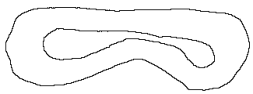
\includegraphics[interpolate=true,width=2.530000in,height=0.940000in]{contents/chapt7/figs/model/cornering_stiffness-img1.png}}%
\end{pgfscope}%
\begin{pgfscope}%
\pgfpathrectangle{\pgfqpoint{2.825000in}{0.508846in}}{\pgfqpoint{2.525000in}{0.932308in}}%
\pgfusepath{clip}%
\pgfsetrectcap%
\pgfsetroundjoin%
\pgfsetlinewidth{1.505625pt}%
\definecolor{currentstroke}{rgb}{0.121569,0.466667,0.705882}%
\pgfsetstrokecolor{currentstroke}%
\pgfsetstrokeopacity{0.700000}%
\pgfsetdash{}{0pt}%
\pgfpathmoveto{\pgfqpoint{4.378846in}{1.208077in}}%
\pgfpathlineto{\pgfqpoint{4.319458in}{1.209146in}}%
\pgfpathlineto{\pgfqpoint{4.272471in}{1.212520in}}%
\pgfpathlineto{\pgfqpoint{4.227084in}{1.217894in}}%
\pgfpathlineto{\pgfqpoint{4.103399in}{1.234024in}}%
\pgfpathlineto{\pgfqpoint{4.056752in}{1.237459in}}%
\pgfpathlineto{\pgfqpoint{4.009985in}{1.238234in}}%
\pgfpathlineto{\pgfqpoint{3.963238in}{1.236617in}}%
\pgfpathlineto{\pgfqpoint{3.807564in}{1.228491in}}%
\pgfpathlineto{\pgfqpoint{3.768613in}{1.229921in}}%
\pgfpathlineto{\pgfqpoint{3.706456in}{1.235074in}}%
\pgfpathlineto{\pgfqpoint{3.644273in}{1.239878in}}%
\pgfpathlineto{\pgfqpoint{3.597516in}{1.241143in}}%
\pgfpathlineto{\pgfqpoint{3.550758in}{1.239981in}}%
\pgfpathlineto{\pgfqpoint{3.504144in}{1.236127in}}%
\pgfpathlineto{\pgfqpoint{3.457827in}{1.229611in}}%
\pgfpathlineto{\pgfqpoint{3.404246in}{1.219267in}}%
\pgfpathlineto{\pgfqpoint{3.351219in}{1.206380in}}%
\pgfpathlineto{\pgfqpoint{3.313826in}{1.195374in}}%
\pgfpathlineto{\pgfqpoint{3.277104in}{1.182312in}}%
\pgfpathlineto{\pgfqpoint{3.248495in}{1.169915in}}%
\pgfpathlineto{\pgfqpoint{3.220980in}{1.155257in}}%
\pgfpathlineto{\pgfqpoint{3.201361in}{1.142532in}}%
\pgfpathlineto{\pgfqpoint{3.182918in}{1.128160in}}%
\pgfpathlineto{\pgfqpoint{3.165930in}{1.112094in}}%
\pgfpathlineto{\pgfqpoint{3.150665in}{1.094386in}}%
\pgfpathlineto{\pgfqpoint{3.137445in}{1.075104in}}%
\pgfpathlineto{\pgfqpoint{3.126537in}{1.054428in}}%
\pgfpathlineto{\pgfqpoint{3.118241in}{1.032574in}}%
\pgfpathlineto{\pgfqpoint{3.112770in}{1.009848in}}%
\pgfpathlineto{\pgfqpoint{3.110226in}{0.986611in}}%
\pgfpathlineto{\pgfqpoint{3.110584in}{0.963237in}}%
\pgfpathlineto{\pgfqpoint{3.113647in}{0.940060in}}%
\pgfpathlineto{\pgfqpoint{3.119320in}{0.917380in}}%
\pgfpathlineto{\pgfqpoint{3.127436in}{0.895456in}}%
\pgfpathlineto{\pgfqpoint{3.137889in}{0.874543in}}%
\pgfpathlineto{\pgfqpoint{3.150571in}{0.854904in}}%
\pgfpathlineto{\pgfqpoint{3.165373in}{0.836808in}}%
\pgfpathlineto{\pgfqpoint{3.182040in}{0.820412in}}%
\pgfpathlineto{\pgfqpoint{3.200364in}{0.805893in}}%
\pgfpathlineto{\pgfqpoint{3.220148in}{0.793435in}}%
\pgfpathlineto{\pgfqpoint{3.241145in}{0.783152in}}%
\pgfpathlineto{\pgfqpoint{3.263105in}{0.775126in}}%
\pgfpathlineto{\pgfqpoint{3.285755in}{0.769320in}}%
\pgfpathlineto{\pgfqpoint{3.308849in}{0.765657in}}%
\pgfpathlineto{\pgfqpoint{3.332164in}{0.763860in}}%
\pgfpathlineto{\pgfqpoint{3.363342in}{0.763925in}}%
\pgfpathlineto{\pgfqpoint{3.394430in}{0.766317in}}%
\pgfpathlineto{\pgfqpoint{3.432983in}{0.772036in}}%
\pgfpathlineto{\pgfqpoint{3.471115in}{0.780114in}}%
\pgfpathlineto{\pgfqpoint{3.531552in}{0.795522in}}%
\pgfpathlineto{\pgfqpoint{3.644736in}{0.824902in}}%
\pgfpathlineto{\pgfqpoint{3.682998in}{0.832342in}}%
\pgfpathlineto{\pgfqpoint{3.721600in}{0.837746in}}%
\pgfpathlineto{\pgfqpoint{3.768213in}{0.841619in}}%
\pgfpathlineto{\pgfqpoint{3.916000in}{0.851400in}}%
\pgfpathlineto{\pgfqpoint{3.977885in}{0.859157in}}%
\pgfpathlineto{\pgfqpoint{4.124660in}{0.879042in}}%
\pgfpathlineto{\pgfqpoint{4.163547in}{0.881694in}}%
\pgfpathlineto{\pgfqpoint{4.202521in}{0.882006in}}%
\pgfpathlineto{\pgfqpoint{4.233652in}{0.880228in}}%
\pgfpathlineto{\pgfqpoint{4.264585in}{0.876316in}}%
\pgfpathlineto{\pgfqpoint{4.295159in}{0.870202in}}%
\pgfpathlineto{\pgfqpoint{4.325250in}{0.862030in}}%
\pgfpathlineto{\pgfqpoint{4.354774in}{0.851999in}}%
\pgfpathlineto{\pgfqpoint{4.390911in}{0.837389in}}%
\pgfpathlineto{\pgfqpoint{4.483490in}{0.796138in}}%
\pgfpathlineto{\pgfqpoint{4.661935in}{0.717831in}}%
\pgfpathlineto{\pgfqpoint{4.712002in}{0.697576in}}%
\pgfpathlineto{\pgfqpoint{4.748264in}{0.685655in}}%
\pgfpathlineto{\pgfqpoint{4.777755in}{0.678723in}}%
\pgfpathlineto{\pgfqpoint{4.800122in}{0.675594in}}%
\pgfpathlineto{\pgfqpoint{4.822584in}{0.674438in}}%
\pgfpathlineto{\pgfqpoint{4.844964in}{0.675399in}}%
\pgfpathlineto{\pgfqpoint{4.867043in}{0.678600in}}%
\pgfpathlineto{\pgfqpoint{4.888598in}{0.684000in}}%
\pgfpathlineto{\pgfqpoint{4.909417in}{0.691507in}}%
\pgfpathlineto{\pgfqpoint{4.929293in}{0.701035in}}%
\pgfpathlineto{\pgfqpoint{4.948351in}{0.712555in}}%
\pgfpathlineto{\pgfqpoint{4.967128in}{0.726060in}}%
\pgfpathlineto{\pgfqpoint{4.990938in}{0.746245in}}%
\pgfpathlineto{\pgfqpoint{5.012828in}{0.768499in}}%
\pgfpathlineto{\pgfqpoint{5.027767in}{0.786528in}}%
\pgfpathlineto{\pgfqpoint{5.041241in}{0.805676in}}%
\pgfpathlineto{\pgfqpoint{5.053051in}{0.825892in}}%
\pgfpathlineto{\pgfqpoint{5.063160in}{0.847010in}}%
\pgfpathlineto{\pgfqpoint{5.071442in}{0.868909in}}%
\pgfpathlineto{\pgfqpoint{5.077755in}{0.891454in}}%
\pgfpathlineto{\pgfqpoint{5.081971in}{0.914483in}}%
\pgfpathlineto{\pgfqpoint{5.084015in}{0.937804in}}%
\pgfpathlineto{\pgfqpoint{5.083654in}{0.961211in}}%
\pgfpathlineto{\pgfqpoint{5.080892in}{0.984458in}}%
\pgfpathlineto{\pgfqpoint{5.075867in}{1.007323in}}%
\pgfpathlineto{\pgfqpoint{5.068580in}{1.029571in}}%
\pgfpathlineto{\pgfqpoint{5.059045in}{1.050951in}}%
\pgfpathlineto{\pgfqpoint{5.047368in}{1.071240in}}%
\pgfpathlineto{\pgfqpoint{5.033619in}{1.090186in}}%
\pgfpathlineto{\pgfqpoint{5.017930in}{1.107560in}}%
\pgfpathlineto{\pgfqpoint{5.000511in}{1.123201in}}%
\pgfpathlineto{\pgfqpoint{4.981659in}{1.137081in}}%
\pgfpathlineto{\pgfqpoint{4.961608in}{1.149169in}}%
\pgfpathlineto{\pgfqpoint{4.940570in}{1.159442in}}%
\pgfpathlineto{\pgfqpoint{4.918771in}{1.167988in}}%
\pgfpathlineto{\pgfqpoint{4.888871in}{1.176957in}}%
\pgfpathlineto{\pgfqpoint{4.858387in}{1.183704in}}%
\pgfpathlineto{\pgfqpoint{4.819897in}{1.190161in}}%
\pgfpathlineto{\pgfqpoint{4.765681in}{1.196973in}}%
\pgfpathlineto{\pgfqpoint{4.695744in}{1.203645in}}%
\pgfpathlineto{\pgfqpoint{4.617870in}{1.209043in}}%
\pgfpathlineto{\pgfqpoint{4.555461in}{1.211271in}}%
\pgfpathlineto{\pgfqpoint{4.493013in}{1.211267in}}%
\pgfpathlineto{\pgfqpoint{4.430583in}{1.209681in}}%
\pgfpathlineto{\pgfqpoint{4.430583in}{1.209681in}}%
\pgfusepath{stroke}%
\end{pgfscope}%
\begin{pgfscope}%
\pgfpathrectangle{\pgfqpoint{2.825000in}{0.508846in}}{\pgfqpoint{2.525000in}{0.932308in}}%
\pgfusepath{clip}%
\pgfsetrectcap%
\pgfsetroundjoin%
\pgfsetlinewidth{1.505625pt}%
\definecolor{currentstroke}{rgb}{1.000000,0.498039,0.054902}%
\pgfsetstrokecolor{currentstroke}%
\pgfsetstrokeopacity{0.700000}%
\pgfsetdash{}{0pt}%
\pgfpathmoveto{\pgfqpoint{4.378846in}{1.208077in}}%
\pgfpathlineto{\pgfqpoint{4.325597in}{1.209062in}}%
\pgfpathlineto{\pgfqpoint{4.286669in}{1.212118in}}%
\pgfpathlineto{\pgfqpoint{4.242734in}{1.217832in}}%
\pgfpathlineto{\pgfqpoint{4.088808in}{1.241428in}}%
\pgfpathlineto{\pgfqpoint{4.042200in}{1.244734in}}%
\pgfpathlineto{\pgfqpoint{3.995489in}{1.245910in}}%
\pgfpathlineto{\pgfqpoint{3.933194in}{1.244988in}}%
\pgfpathlineto{\pgfqpoint{3.808621in}{1.242180in}}%
\pgfpathlineto{\pgfqpoint{3.746333in}{1.243514in}}%
\pgfpathlineto{\pgfqpoint{3.652898in}{1.245449in}}%
\pgfpathlineto{\pgfqpoint{3.606181in}{1.244540in}}%
\pgfpathlineto{\pgfqpoint{3.559566in}{1.241361in}}%
\pgfpathlineto{\pgfqpoint{3.513169in}{1.235835in}}%
\pgfpathlineto{\pgfqpoint{3.467113in}{1.227965in}}%
\pgfpathlineto{\pgfqpoint{3.421483in}{1.217905in}}%
\pgfpathlineto{\pgfqpoint{3.368805in}{1.203882in}}%
\pgfpathlineto{\pgfqpoint{3.324230in}{1.189870in}}%
\pgfpathlineto{\pgfqpoint{3.280439in}{1.173580in}}%
\pgfpathlineto{\pgfqpoint{3.252016in}{1.160842in}}%
\pgfpathlineto{\pgfqpoint{3.224670in}{1.145939in}}%
\pgfpathlineto{\pgfqpoint{3.205194in}{1.133043in}}%
\pgfpathlineto{\pgfqpoint{3.186939in}{1.118473in}}%
\pgfpathlineto{\pgfqpoint{3.170268in}{1.102115in}}%
\pgfpathlineto{\pgfqpoint{3.155522in}{1.084008in}}%
\pgfpathlineto{\pgfqpoint{3.143104in}{1.064232in}}%
\pgfpathlineto{\pgfqpoint{3.133339in}{1.043023in}}%
\pgfpathlineto{\pgfqpoint{3.126434in}{1.020718in}}%
\pgfpathlineto{\pgfqpoint{3.122600in}{0.997687in}}%
\pgfpathlineto{\pgfqpoint{3.121883in}{0.974348in}}%
\pgfpathlineto{\pgfqpoint{3.124167in}{0.951108in}}%
\pgfpathlineto{\pgfqpoint{3.129156in}{0.928295in}}%
\pgfpathlineto{\pgfqpoint{3.136693in}{0.906190in}}%
\pgfpathlineto{\pgfqpoint{3.146624in}{0.885052in}}%
\pgfpathlineto{\pgfqpoint{3.158800in}{0.865123in}}%
\pgfpathlineto{\pgfqpoint{3.173098in}{0.846657in}}%
\pgfpathlineto{\pgfqpoint{3.189396in}{0.829930in}}%
\pgfpathlineto{\pgfqpoint{3.207470in}{0.815141in}}%
\pgfpathlineto{\pgfqpoint{3.227126in}{0.802531in}}%
\pgfpathlineto{\pgfqpoint{3.248119in}{0.792300in}}%
\pgfpathlineto{\pgfqpoint{3.270137in}{0.784513in}}%
\pgfpathlineto{\pgfqpoint{3.292854in}{0.779087in}}%
\pgfpathlineto{\pgfqpoint{3.315992in}{0.775895in}}%
\pgfpathlineto{\pgfqpoint{3.339322in}{0.774738in}}%
\pgfpathlineto{\pgfqpoint{3.370455in}{0.775630in}}%
\pgfpathlineto{\pgfqpoint{3.409207in}{0.779414in}}%
\pgfpathlineto{\pgfqpoint{3.470871in}{0.788318in}}%
\pgfpathlineto{\pgfqpoint{3.547678in}{0.801197in}}%
\pgfpathlineto{\pgfqpoint{3.624106in}{0.816165in}}%
\pgfpathlineto{\pgfqpoint{3.700517in}{0.831204in}}%
\pgfpathlineto{\pgfqpoint{3.746756in}{0.837924in}}%
\pgfpathlineto{\pgfqpoint{3.793259in}{0.842485in}}%
\pgfpathlineto{\pgfqpoint{3.925157in}{0.853826in}}%
\pgfpathlineto{\pgfqpoint{3.986840in}{0.862589in}}%
\pgfpathlineto{\pgfqpoint{4.102330in}{0.880123in}}%
\pgfpathlineto{\pgfqpoint{4.148847in}{0.884507in}}%
\pgfpathlineto{\pgfqpoint{4.187762in}{0.885711in}}%
\pgfpathlineto{\pgfqpoint{4.218891in}{0.884621in}}%
\pgfpathlineto{\pgfqpoint{4.249887in}{0.881549in}}%
\pgfpathlineto{\pgfqpoint{4.280634in}{0.876571in}}%
\pgfpathlineto{\pgfqpoint{4.311020in}{0.869719in}}%
\pgfpathlineto{\pgfqpoint{4.348399in}{0.858822in}}%
\pgfpathlineto{\pgfqpoint{4.385051in}{0.845685in}}%
\pgfpathlineto{\pgfqpoint{4.428044in}{0.827385in}}%
\pgfpathlineto{\pgfqpoint{4.484321in}{0.800656in}}%
\pgfpathlineto{\pgfqpoint{4.560653in}{0.761767in}}%
\pgfpathlineto{\pgfqpoint{4.637123in}{0.723151in}}%
\pgfpathlineto{\pgfqpoint{4.679798in}{0.704161in}}%
\pgfpathlineto{\pgfqpoint{4.708796in}{0.693291in}}%
\pgfpathlineto{\pgfqpoint{4.738302in}{0.684595in}}%
\pgfpathlineto{\pgfqpoint{4.760742in}{0.679846in}}%
\pgfpathlineto{\pgfqpoint{4.783372in}{0.676904in}}%
\pgfpathlineto{\pgfqpoint{4.806059in}{0.676054in}}%
\pgfpathlineto{\pgfqpoint{4.828717in}{0.677418in}}%
\pgfpathlineto{\pgfqpoint{4.851823in}{0.681049in}}%
\pgfpathlineto{\pgfqpoint{4.874639in}{0.686633in}}%
\pgfpathlineto{\pgfqpoint{4.896906in}{0.694114in}}%
\pgfpathlineto{\pgfqpoint{4.918473in}{0.703422in}}%
\pgfpathlineto{\pgfqpoint{4.939168in}{0.714533in}}%
\pgfpathlineto{\pgfqpoint{4.958823in}{0.727394in}}%
\pgfpathlineto{\pgfqpoint{4.977273in}{0.741932in}}%
\pgfpathlineto{\pgfqpoint{4.994463in}{0.757940in}}%
\pgfpathlineto{\pgfqpoint{5.010224in}{0.775356in}}%
\pgfpathlineto{\pgfqpoint{5.024460in}{0.794040in}}%
\pgfpathlineto{\pgfqpoint{5.037017in}{0.813891in}}%
\pgfpathlineto{\pgfqpoint{5.047804in}{0.834757in}}%
\pgfpathlineto{\pgfqpoint{5.056708in}{0.856493in}}%
\pgfpathlineto{\pgfqpoint{5.063614in}{0.878942in}}%
\pgfpathlineto{\pgfqpoint{5.068246in}{0.901968in}}%
\pgfpathlineto{\pgfqpoint{5.070506in}{0.925345in}}%
\pgfpathlineto{\pgfqpoint{5.070262in}{0.948829in}}%
\pgfpathlineto{\pgfqpoint{5.067435in}{0.972143in}}%
\pgfpathlineto{\pgfqpoint{5.061967in}{0.994981in}}%
\pgfpathlineto{\pgfqpoint{5.053889in}{1.017021in}}%
\pgfpathlineto{\pgfqpoint{5.043379in}{1.037924in}}%
\pgfpathlineto{\pgfqpoint{5.030552in}{1.057384in}}%
\pgfpathlineto{\pgfqpoint{5.015588in}{1.075137in}}%
\pgfpathlineto{\pgfqpoint{4.998690in}{1.090930in}}%
\pgfpathlineto{\pgfqpoint{4.980149in}{1.104612in}}%
\pgfpathlineto{\pgfqpoint{4.960286in}{1.116119in}}%
\pgfpathlineto{\pgfqpoint{4.939119in}{1.125591in}}%
\pgfpathlineto{\pgfqpoint{4.909679in}{1.135663in}}%
\pgfpathlineto{\pgfqpoint{4.864585in}{1.147740in}}%
\pgfpathlineto{\pgfqpoint{4.804522in}{1.164060in}}%
\pgfpathlineto{\pgfqpoint{4.767664in}{1.176501in}}%
\pgfpathlineto{\pgfqpoint{4.672420in}{1.210484in}}%
\pgfpathlineto{\pgfqpoint{4.642246in}{1.218091in}}%
\pgfpathlineto{\pgfqpoint{4.611612in}{1.223561in}}%
\pgfpathlineto{\pgfqpoint{4.580686in}{1.227031in}}%
\pgfpathlineto{\pgfqpoint{4.541836in}{1.228982in}}%
\pgfpathlineto{\pgfqpoint{4.495155in}{1.228711in}}%
\pgfpathlineto{\pgfqpoint{4.417363in}{1.227487in}}%
\pgfpathlineto{\pgfqpoint{4.378513in}{1.229421in}}%
\pgfpathlineto{\pgfqpoint{4.378513in}{1.229421in}}%
\pgfusepath{stroke}%
\end{pgfscope}%
\begin{pgfscope}%
\definecolor{textcolor}{rgb}{0.000000,0.000000,0.000000}%
\pgfsetstrokecolor{textcolor}%
\pgfsetfillcolor{textcolor}%
\pgftext[x=4.087500in,y=1.524487in,,base]{\color{textcolor}\rmfamily\fontsize{12.000000}{14.400000}\selectfont Steering and velocity controllers}%
\end{pgfscope}%
\begin{pgfscope}%
\pgfsetbuttcap%
\pgfsetmiterjoin%
\definecolor{currentfill}{rgb}{1.000000,1.000000,1.000000}%
\pgfsetfillcolor{currentfill}%
\pgfsetfillopacity{0.800000}%
\pgfsetlinewidth{1.003750pt}%
\definecolor{currentstroke}{rgb}{0.800000,0.800000,0.800000}%
\pgfsetstrokecolor{currentstroke}%
\pgfsetstrokeopacity{0.800000}%
\pgfsetdash{}{0pt}%
\pgfpathmoveto{\pgfqpoint{0.937900in}{0.069444in}}%
\pgfpathlineto{\pgfqpoint{4.562100in}{0.069444in}}%
\pgfpathquadraticcurveto{\pgfqpoint{4.589878in}{0.069444in}}{\pgfqpoint{4.589878in}{0.097222in}}%
\pgfpathlineto{\pgfqpoint{4.589878in}{0.444675in}}%
\pgfpathquadraticcurveto{\pgfqpoint{4.589878in}{0.472452in}}{\pgfqpoint{4.562100in}{0.472452in}}%
\pgfpathlineto{\pgfqpoint{0.937900in}{0.472452in}}%
\pgfpathquadraticcurveto{\pgfqpoint{0.910122in}{0.472452in}}{\pgfqpoint{0.910122in}{0.444675in}}%
\pgfpathlineto{\pgfqpoint{0.910122in}{0.097222in}}%
\pgfpathquadraticcurveto{\pgfqpoint{0.910122in}{0.069444in}}{\pgfqpoint{0.937900in}{0.069444in}}%
\pgfpathlineto{\pgfqpoint{0.937900in}{0.069444in}}%
\pgfpathclose%
\pgfusepath{stroke,fill}%
\end{pgfscope}%
\begin{pgfscope}%
\pgfsetrectcap%
\pgfsetroundjoin%
\pgfsetlinewidth{1.505625pt}%
\definecolor{currentstroke}{rgb}{0.121569,0.466667,0.705882}%
\pgfsetstrokecolor{currentstroke}%
\pgfsetstrokeopacity{0.700000}%
\pgfsetdash{}{0pt}%
\pgfpathmoveto{\pgfqpoint{0.965678in}{0.266798in}}%
\pgfpathlineto{\pgfqpoint{1.104567in}{0.266798in}}%
\pgfpathlineto{\pgfqpoint{1.243456in}{0.266798in}}%
\pgfusepath{stroke}%
\end{pgfscope}%
\begin{pgfscope}%
\definecolor{textcolor}{rgb}{0.000000,0.000000,0.000000}%
\pgfsetstrokecolor{textcolor}%
\pgfsetfillcolor{textcolor}%
\pgftext[x=1.354567in,y=0.218187in,left,base]{\color{textcolor}\rmfamily\fontsize{10.000000}{12.000000}\selectfont No model error}%
\end{pgfscope}%
\begin{pgfscope}%
\pgfsetrectcap%
\pgfsetroundjoin%
\pgfsetlinewidth{1.505625pt}%
\definecolor{currentstroke}{rgb}{1.000000,0.498039,0.054902}%
\pgfsetstrokecolor{currentstroke}%
\pgfsetstrokeopacity{0.700000}%
\pgfsetdash{}{0pt}%
\pgfpathmoveto{\pgfqpoint{2.721619in}{0.266798in}}%
\pgfpathlineto{\pgfqpoint{2.860508in}{0.266798in}}%
\pgfpathlineto{\pgfqpoint{2.999396in}{0.266798in}}%
\pgfusepath{stroke}%
\end{pgfscope}%
\begin{pgfscope}%
\definecolor{textcolor}{rgb}{0.000000,0.000000,0.000000}%
\pgfsetstrokecolor{textcolor}%
\pgfsetfillcolor{textcolor}%
\pgftext[x=3.110507in, y=0.311374in, left, base]{\color{textcolor}\rmfamily\fontsize{10.000000}{12.000000}\selectfont Increased front tire }%
\end{pgfscope}%
\begin{pgfscope}%
\definecolor{textcolor}{rgb}{0.000000,0.000000,0.000000}%
\pgfsetstrokecolor{textcolor}%
\pgfsetfillcolor{textcolor}%
\pgftext[x=3.110507in, y=0.155856in, left, base]{\color{textcolor}\rmfamily\fontsize{10.000000}{12.000000}\selectfont cornering stiffness}%
\end{pgfscope}%
\end{pgfpicture}%
\makeatother%
\endgroup%

    \caption[Paths taken by agents with no model error, and with an increased tire front tire stiffness coefficient]{Paths taken by agents with no model error, and with an increased tire front tire stiffness coefficient.}
    \label{fig:front_cornering_stiffness_+_paths}
\end{figure}

Although Figure \ref{fig:front_cornering_stiffness_+_paths} indicates that the end-to-end agent complete laps successfully when the front tire cornering stiffness is lower than expected, the behaviour of this agent is still dangerous.
Figure \ref{fig:front_cornering_stiffness_-_paths} shows the paths taken by the end-to-end and partial end-to-end agents with a front tire cornering stiffness of $4.01$, which is $15\%$ smaller than the nominal value of $4.72$.
We see from this figure that decreasing the front tire cornering stiffness causes end-to-end agents to understeer and drive wide around the corners.
However, our partial end-to-end agent follows a very similar path to the one it had taken without the decreased front tire cornering stiffness.

\begin{figure}[htb!]
    \centering
    %% Creator: Matplotlib, PGF backend
%%
%% To include the figure in your LaTeX document, write
%%   \input{<filename>.pgf}
%%
%% Make sure the required packages are loaded in your preamble
%%   \usepackage{pgf}
%%
%% Also ensure that all the required font packages are loaded; for instance,
%% the lmodern package is sometimes necessary when using math font.
%%   \usepackage{lmodern}
%%
%% Figures using additional raster images can only be included by \input if
%% they are in the same directory as the main LaTeX file. For loading figures
%% from other directories you can use the `import` package
%%   \usepackage{import}
%%
%% and then include the figures with
%%   \import{<path to file>}{<filename>.pgf}
%%
%% Matplotlib used the following preamble
%%   \usepackage{fontspec}
%%   \setmainfont{DejaVuSerif.ttf}[Path=\detokenize{/home/andrew/anaconda3/envs/auto_car_env/lib/python3.9/site-packages/matplotlib/mpl-data/fonts/ttf/}]
%%   \setsansfont{DejaVuSans.ttf}[Path=\detokenize{/home/andrew/anaconda3/envs/auto_car_env/lib/python3.9/site-packages/matplotlib/mpl-data/fonts/ttf/}]
%%   \setmonofont{DejaVuSansMono.ttf}[Path=\detokenize{/home/andrew/anaconda3/envs/auto_car_env/lib/python3.9/site-packages/matplotlib/mpl-data/fonts/ttf/}]
%%
\begingroup%
\makeatletter%
\begin{pgfpicture}%
\pgfpathrectangle{\pgfpointorigin}{\pgfqpoint{5.500000in}{2.000000in}}%
\pgfusepath{use as bounding box, clip}%
\begin{pgfscope}%
\pgfsetbuttcap%
\pgfsetmiterjoin%
\definecolor{currentfill}{rgb}{1.000000,1.000000,1.000000}%
\pgfsetfillcolor{currentfill}%
\pgfsetlinewidth{0.000000pt}%
\definecolor{currentstroke}{rgb}{1.000000,1.000000,1.000000}%
\pgfsetstrokecolor{currentstroke}%
\pgfsetdash{}{0pt}%
\pgfpathmoveto{\pgfqpoint{0.000000in}{0.000000in}}%
\pgfpathlineto{\pgfqpoint{5.500000in}{0.000000in}}%
\pgfpathlineto{\pgfqpoint{5.500000in}{2.000000in}}%
\pgfpathlineto{\pgfqpoint{0.000000in}{2.000000in}}%
\pgfpathlineto{\pgfqpoint{0.000000in}{0.000000in}}%
\pgfpathclose%
\pgfusepath{fill}%
\end{pgfscope}%
\begin{pgfscope}%
\pgfpathrectangle{\pgfqpoint{0.150000in}{0.508846in}}{\pgfqpoint{2.525000in}{0.932308in}}%
\pgfusepath{clip}%
\pgfsys@transformshift{0.150000in}{0.508846in}%
\pgftext[left,bottom]{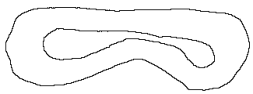
\includegraphics[interpolate=true,width=2.530000in,height=0.940000in]{contents/chapt7/figs/model/front_cornering_stiffness_path-img0.png}}%
\end{pgfscope}%
\begin{pgfscope}%
\pgfpathrectangle{\pgfqpoint{0.150000in}{0.508846in}}{\pgfqpoint{2.525000in}{0.932308in}}%
\pgfusepath{clip}%
\pgfsetrectcap%
\pgfsetroundjoin%
\pgfsetlinewidth{1.505625pt}%
\definecolor{currentstroke}{rgb}{0.121569,0.466667,0.705882}%
\pgfsetstrokecolor{currentstroke}%
\pgfsetstrokeopacity{0.700000}%
\pgfsetdash{}{0pt}%
\pgfpathmoveto{\pgfqpoint{1.703846in}{1.208077in}}%
\pgfpathlineto{\pgfqpoint{1.638569in}{1.209062in}}%
\pgfpathlineto{\pgfqpoint{1.575430in}{1.212385in}}%
\pgfpathlineto{\pgfqpoint{1.483510in}{1.219816in}}%
\pgfpathlineto{\pgfqpoint{1.354939in}{1.230699in}}%
\pgfpathlineto{\pgfqpoint{1.292804in}{1.233459in}}%
\pgfpathlineto{\pgfqpoint{1.199513in}{1.234666in}}%
\pgfpathlineto{\pgfqpoint{0.950723in}{1.234867in}}%
\pgfpathlineto{\pgfqpoint{0.888579in}{1.232311in}}%
\pgfpathlineto{\pgfqpoint{0.834320in}{1.228104in}}%
\pgfpathlineto{\pgfqpoint{0.780266in}{1.221790in}}%
\pgfpathlineto{\pgfqpoint{0.726518in}{1.213259in}}%
\pgfpathlineto{\pgfqpoint{0.673176in}{1.202475in}}%
\pgfpathlineto{\pgfqpoint{0.635569in}{1.192658in}}%
\pgfpathlineto{\pgfqpoint{0.606206in}{1.182438in}}%
\pgfpathlineto{\pgfqpoint{0.584904in}{1.172951in}}%
\pgfpathlineto{\pgfqpoint{0.564485in}{1.161690in}}%
\pgfpathlineto{\pgfqpoint{0.545258in}{1.148502in}}%
\pgfpathlineto{\pgfqpoint{0.527551in}{1.133337in}}%
\pgfpathlineto{\pgfqpoint{0.511810in}{1.116142in}}%
\pgfpathlineto{\pgfqpoint{0.498378in}{1.097091in}}%
\pgfpathlineto{\pgfqpoint{0.487604in}{1.076421in}}%
\pgfpathlineto{\pgfqpoint{0.479780in}{1.054465in}}%
\pgfpathlineto{\pgfqpoint{0.475155in}{1.031622in}}%
\pgfpathlineto{\pgfqpoint{0.473924in}{1.016125in}}%
\pgfpathlineto{\pgfqpoint{0.474846in}{0.992835in}}%
\pgfpathlineto{\pgfqpoint{0.478822in}{0.969865in}}%
\pgfpathlineto{\pgfqpoint{0.485533in}{0.947539in}}%
\pgfpathlineto{\pgfqpoint{0.494754in}{0.926126in}}%
\pgfpathlineto{\pgfqpoint{0.506184in}{0.905803in}}%
\pgfpathlineto{\pgfqpoint{0.519553in}{0.886700in}}%
\pgfpathlineto{\pgfqpoint{0.534611in}{0.868895in}}%
\pgfpathlineto{\pgfqpoint{0.551064in}{0.852369in}}%
\pgfpathlineto{\pgfqpoint{0.568700in}{0.837111in}}%
\pgfpathlineto{\pgfqpoint{0.593788in}{0.818747in}}%
\pgfpathlineto{\pgfqpoint{0.620360in}{0.802604in}}%
\pgfpathlineto{\pgfqpoint{0.648143in}{0.788644in}}%
\pgfpathlineto{\pgfqpoint{0.676922in}{0.776876in}}%
\pgfpathlineto{\pgfqpoint{0.706548in}{0.767440in}}%
\pgfpathlineto{\pgfqpoint{0.736838in}{0.760426in}}%
\pgfpathlineto{\pgfqpoint{0.767604in}{0.755939in}}%
\pgfpathlineto{\pgfqpoint{0.798639in}{0.754071in}}%
\pgfpathlineto{\pgfqpoint{0.829720in}{0.754854in}}%
\pgfpathlineto{\pgfqpoint{0.860651in}{0.758030in}}%
\pgfpathlineto{\pgfqpoint{0.891266in}{0.763462in}}%
\pgfpathlineto{\pgfqpoint{0.921440in}{0.770972in}}%
\pgfpathlineto{\pgfqpoint{0.951075in}{0.780390in}}%
\pgfpathlineto{\pgfqpoint{0.987261in}{0.794578in}}%
\pgfpathlineto{\pgfqpoint{1.036795in}{0.817118in}}%
\pgfpathlineto{\pgfqpoint{1.156416in}{0.873316in}}%
\pgfpathlineto{\pgfqpoint{1.206728in}{0.894064in}}%
\pgfpathlineto{\pgfqpoint{1.257830in}{0.912777in}}%
\pgfpathlineto{\pgfqpoint{1.302320in}{0.926794in}}%
\pgfpathlineto{\pgfqpoint{1.347441in}{0.938617in}}%
\pgfpathlineto{\pgfqpoint{1.393137in}{0.947973in}}%
\pgfpathlineto{\pgfqpoint{1.431589in}{0.953662in}}%
\pgfpathlineto{\pgfqpoint{1.470302in}{0.957147in}}%
\pgfpathlineto{\pgfqpoint{1.509155in}{0.958246in}}%
\pgfpathlineto{\pgfqpoint{1.547997in}{0.956817in}}%
\pgfpathlineto{\pgfqpoint{1.586669in}{0.952902in}}%
\pgfpathlineto{\pgfqpoint{1.625078in}{0.946929in}}%
\pgfpathlineto{\pgfqpoint{1.670742in}{0.937412in}}%
\pgfpathlineto{\pgfqpoint{1.715828in}{0.925781in}}%
\pgfpathlineto{\pgfqpoint{1.752216in}{0.914251in}}%
\pgfpathlineto{\pgfqpoint{1.787134in}{0.900659in}}%
\pgfpathlineto{\pgfqpoint{1.813785in}{0.888073in}}%
\pgfpathlineto{\pgfqpoint{1.839081in}{0.873840in}}%
\pgfpathlineto{\pgfqpoint{1.862799in}{0.858171in}}%
\pgfpathlineto{\pgfqpoint{1.884854in}{0.841356in}}%
\pgfpathlineto{\pgfqpoint{1.905204in}{0.823546in}}%
\pgfpathlineto{\pgfqpoint{1.928294in}{0.800213in}}%
\pgfpathlineto{\pgfqpoint{1.949038in}{0.775868in}}%
\pgfpathlineto{\pgfqpoint{2.003406in}{0.708335in}}%
\pgfpathlineto{\pgfqpoint{2.027702in}{0.683217in}}%
\pgfpathlineto{\pgfqpoint{2.049177in}{0.664214in}}%
\pgfpathlineto{\pgfqpoint{2.066731in}{0.651011in}}%
\pgfpathlineto{\pgfqpoint{2.085643in}{0.639090in}}%
\pgfpathlineto{\pgfqpoint{2.105881in}{0.628706in}}%
\pgfpathlineto{\pgfqpoint{2.127382in}{0.620158in}}%
\pgfpathlineto{\pgfqpoint{2.149888in}{0.613760in}}%
\pgfpathlineto{\pgfqpoint{2.172954in}{0.609840in}}%
\pgfpathlineto{\pgfqpoint{2.196315in}{0.608579in}}%
\pgfpathlineto{\pgfqpoint{2.219655in}{0.610173in}}%
\pgfpathlineto{\pgfqpoint{2.242596in}{0.614745in}}%
\pgfpathlineto{\pgfqpoint{2.264738in}{0.622290in}}%
\pgfpathlineto{\pgfqpoint{2.285665in}{0.632741in}}%
\pgfpathlineto{\pgfqpoint{2.304984in}{0.645928in}}%
\pgfpathlineto{\pgfqpoint{2.322303in}{0.661589in}}%
\pgfpathlineto{\pgfqpoint{2.337460in}{0.679272in}}%
\pgfpathlineto{\pgfqpoint{2.350468in}{0.698519in}}%
\pgfpathlineto{\pgfqpoint{2.361443in}{0.718923in}}%
\pgfpathlineto{\pgfqpoint{2.370469in}{0.740196in}}%
\pgfpathlineto{\pgfqpoint{2.377729in}{0.762069in}}%
\pgfpathlineto{\pgfqpoint{2.384950in}{0.791849in}}%
\pgfpathlineto{\pgfqpoint{2.389579in}{0.822106in}}%
\pgfpathlineto{\pgfqpoint{2.391822in}{0.852602in}}%
\pgfpathlineto{\pgfqpoint{2.391785in}{0.883149in}}%
\pgfpathlineto{\pgfqpoint{2.389515in}{0.913581in}}%
\pgfpathlineto{\pgfqpoint{2.385030in}{0.943846in}}%
\pgfpathlineto{\pgfqpoint{2.378039in}{0.974122in}}%
\pgfpathlineto{\pgfqpoint{2.370865in}{0.996379in}}%
\pgfpathlineto{\pgfqpoint{2.361903in}{1.017977in}}%
\pgfpathlineto{\pgfqpoint{2.351038in}{1.038681in}}%
\pgfpathlineto{\pgfqpoint{2.338158in}{1.058193in}}%
\pgfpathlineto{\pgfqpoint{2.323255in}{1.076207in}}%
\pgfpathlineto{\pgfqpoint{2.306511in}{1.092525in}}%
\pgfpathlineto{\pgfqpoint{2.288252in}{1.107131in}}%
\pgfpathlineto{\pgfqpoint{2.268736in}{1.120011in}}%
\pgfpathlineto{\pgfqpoint{2.248194in}{1.131183in}}%
\pgfpathlineto{\pgfqpoint{2.226840in}{1.140716in}}%
\pgfpathlineto{\pgfqpoint{2.197428in}{1.151053in}}%
\pgfpathlineto{\pgfqpoint{2.167277in}{1.159000in}}%
\pgfpathlineto{\pgfqpoint{2.129033in}{1.166526in}}%
\pgfpathlineto{\pgfqpoint{2.082701in}{1.172943in}}%
\pgfpathlineto{\pgfqpoint{2.020617in}{1.178900in}}%
\pgfpathlineto{\pgfqpoint{1.795380in}{1.198517in}}%
\pgfpathlineto{\pgfqpoint{1.741164in}{1.204772in}}%
\pgfpathlineto{\pgfqpoint{1.741164in}{1.204772in}}%
\pgfusepath{stroke}%
\end{pgfscope}%
\begin{pgfscope}%
\pgfpathrectangle{\pgfqpoint{0.150000in}{0.508846in}}{\pgfqpoint{2.525000in}{0.932308in}}%
\pgfusepath{clip}%
\pgfsetrectcap%
\pgfsetroundjoin%
\pgfsetlinewidth{1.505625pt}%
\definecolor{currentstroke}{rgb}{1.000000,0.498039,0.054902}%
\pgfsetstrokecolor{currentstroke}%
\pgfsetstrokeopacity{0.700000}%
\pgfsetdash{}{0pt}%
\pgfpathmoveto{\pgfqpoint{1.703846in}{1.208077in}}%
\pgfpathlineto{\pgfqpoint{1.633346in}{1.209134in}}%
\pgfpathlineto{\pgfqpoint{1.569973in}{1.212330in}}%
\pgfpathlineto{\pgfqpoint{1.470467in}{1.219771in}}%
\pgfpathlineto{\pgfqpoint{1.355652in}{1.228411in}}%
\pgfpathlineto{\pgfqpoint{1.285102in}{1.231223in}}%
\pgfpathlineto{\pgfqpoint{1.136115in}{1.235793in}}%
\pgfpathlineto{\pgfqpoint{0.979412in}{1.243696in}}%
\pgfpathlineto{\pgfqpoint{0.924497in}{1.243722in}}%
\pgfpathlineto{\pgfqpoint{0.877472in}{1.241669in}}%
\pgfpathlineto{\pgfqpoint{0.830591in}{1.237459in}}%
\pgfpathlineto{\pgfqpoint{0.783933in}{1.231244in}}%
\pgfpathlineto{\pgfqpoint{0.729843in}{1.221760in}}%
\pgfpathlineto{\pgfqpoint{0.676163in}{1.210176in}}%
\pgfpathlineto{\pgfqpoint{0.638204in}{1.200296in}}%
\pgfpathlineto{\pgfqpoint{0.608379in}{1.190550in}}%
\pgfpathlineto{\pgfqpoint{0.579425in}{1.178472in}}%
\pgfpathlineto{\pgfqpoint{0.558544in}{1.167622in}}%
\pgfpathlineto{\pgfqpoint{0.538640in}{1.155072in}}%
\pgfpathlineto{\pgfqpoint{0.519965in}{1.140761in}}%
\pgfpathlineto{\pgfqpoint{0.502862in}{1.124605in}}%
\pgfpathlineto{\pgfqpoint{0.487594in}{1.106706in}}%
\pgfpathlineto{\pgfqpoint{0.474433in}{1.087207in}}%
\pgfpathlineto{\pgfqpoint{0.463612in}{1.066318in}}%
\pgfpathlineto{\pgfqpoint{0.455346in}{1.044295in}}%
\pgfpathlineto{\pgfqpoint{0.449780in}{1.021439in}}%
\pgfpathlineto{\pgfqpoint{0.446888in}{0.998091in}}%
\pgfpathlineto{\pgfqpoint{0.446588in}{0.974566in}}%
\pgfpathlineto{\pgfqpoint{0.448819in}{0.951146in}}%
\pgfpathlineto{\pgfqpoint{0.453480in}{0.928084in}}%
\pgfpathlineto{\pgfqpoint{0.460430in}{0.905606in}}%
\pgfpathlineto{\pgfqpoint{0.469550in}{0.883917in}}%
\pgfpathlineto{\pgfqpoint{0.480700in}{0.863198in}}%
\pgfpathlineto{\pgfqpoint{0.493645in}{0.843547in}}%
\pgfpathlineto{\pgfqpoint{0.508062in}{0.824949in}}%
\pgfpathlineto{\pgfqpoint{0.529242in}{0.801805in}}%
\pgfpathlineto{\pgfqpoint{0.552279in}{0.780506in}}%
\pgfpathlineto{\pgfqpoint{0.576813in}{0.760947in}}%
\pgfpathlineto{\pgfqpoint{0.602623in}{0.743105in}}%
\pgfpathlineto{\pgfqpoint{0.629649in}{0.727167in}}%
\pgfpathlineto{\pgfqpoint{0.657773in}{0.713258in}}%
\pgfpathlineto{\pgfqpoint{0.686885in}{0.701559in}}%
\pgfpathlineto{\pgfqpoint{0.716842in}{0.692239in}}%
\pgfpathlineto{\pgfqpoint{0.747467in}{0.685427in}}%
\pgfpathlineto{\pgfqpoint{0.778556in}{0.681209in}}%
\pgfpathlineto{\pgfqpoint{0.809890in}{0.679638in}}%
\pgfpathlineto{\pgfqpoint{0.841244in}{0.680731in}}%
\pgfpathlineto{\pgfqpoint{0.872392in}{0.684485in}}%
\pgfpathlineto{\pgfqpoint{0.903140in}{0.690732in}}%
\pgfpathlineto{\pgfqpoint{0.933414in}{0.698981in}}%
\pgfpathlineto{\pgfqpoint{0.970515in}{0.711701in}}%
\pgfpathlineto{\pgfqpoint{1.006804in}{0.726587in}}%
\pgfpathlineto{\pgfqpoint{1.049398in}{0.746620in}}%
\pgfpathlineto{\pgfqpoint{1.119191in}{0.782452in}}%
\pgfpathlineto{\pgfqpoint{1.244673in}{0.847233in}}%
\pgfpathlineto{\pgfqpoint{1.329303in}{0.888477in}}%
\pgfpathlineto{\pgfqpoint{1.386637in}{0.914005in}}%
\pgfpathlineto{\pgfqpoint{1.430396in}{0.931345in}}%
\pgfpathlineto{\pgfqpoint{1.474897in}{0.946678in}}%
\pgfpathlineto{\pgfqpoint{1.512684in}{0.957192in}}%
\pgfpathlineto{\pgfqpoint{1.543362in}{0.963783in}}%
\pgfpathlineto{\pgfqpoint{1.574381in}{0.968506in}}%
\pgfpathlineto{\pgfqpoint{1.605611in}{0.971176in}}%
\pgfpathlineto{\pgfqpoint{1.636520in}{0.971744in}}%
\pgfpathlineto{\pgfqpoint{1.666866in}{0.970192in}}%
\pgfpathlineto{\pgfqpoint{1.696494in}{0.966499in}}%
\pgfpathlineto{\pgfqpoint{1.725246in}{0.960716in}}%
\pgfpathlineto{\pgfqpoint{1.752974in}{0.952939in}}%
\pgfpathlineto{\pgfqpoint{1.779527in}{0.943302in}}%
\pgfpathlineto{\pgfqpoint{1.804782in}{0.931944in}}%
\pgfpathlineto{\pgfqpoint{1.828641in}{0.919018in}}%
\pgfpathlineto{\pgfqpoint{1.851023in}{0.904682in}}%
\pgfpathlineto{\pgfqpoint{1.871846in}{0.889116in}}%
\pgfpathlineto{\pgfqpoint{1.895553in}{0.868786in}}%
\pgfpathlineto{\pgfqpoint{1.920811in}{0.843876in}}%
\pgfpathlineto{\pgfqpoint{1.946368in}{0.814911in}}%
\pgfpathlineto{\pgfqpoint{2.008897in}{0.740247in}}%
\pgfpathlineto{\pgfqpoint{2.031991in}{0.718390in}}%
\pgfpathlineto{\pgfqpoint{2.052722in}{0.701654in}}%
\pgfpathlineto{\pgfqpoint{2.075730in}{0.686095in}}%
\pgfpathlineto{\pgfqpoint{2.101027in}{0.672110in}}%
\pgfpathlineto{\pgfqpoint{2.128561in}{0.660106in}}%
\pgfpathlineto{\pgfqpoint{2.150601in}{0.652627in}}%
\pgfpathlineto{\pgfqpoint{2.173348in}{0.646784in}}%
\pgfpathlineto{\pgfqpoint{2.196494in}{0.642807in}}%
\pgfpathlineto{\pgfqpoint{2.219902in}{0.640917in}}%
\pgfpathlineto{\pgfqpoint{2.243381in}{0.641294in}}%
\pgfpathlineto{\pgfqpoint{2.266697in}{0.644084in}}%
\pgfpathlineto{\pgfqpoint{2.289582in}{0.649341in}}%
\pgfpathlineto{\pgfqpoint{2.311752in}{0.657076in}}%
\pgfpathlineto{\pgfqpoint{2.332955in}{0.667165in}}%
\pgfpathlineto{\pgfqpoint{2.353055in}{0.679309in}}%
\pgfpathlineto{\pgfqpoint{2.371913in}{0.693304in}}%
\pgfpathlineto{\pgfqpoint{2.389420in}{0.708958in}}%
\pgfpathlineto{\pgfqpoint{2.405525in}{0.726051in}}%
\pgfpathlineto{\pgfqpoint{2.420181in}{0.744403in}}%
\pgfpathlineto{\pgfqpoint{2.433359in}{0.763843in}}%
\pgfpathlineto{\pgfqpoint{2.445014in}{0.784234in}}%
\pgfpathlineto{\pgfqpoint{2.455115in}{0.805437in}}%
\pgfpathlineto{\pgfqpoint{2.463613in}{0.827332in}}%
\pgfpathlineto{\pgfqpoint{2.470479in}{0.849793in}}%
\pgfpathlineto{\pgfqpoint{2.475671in}{0.872698in}}%
\pgfpathlineto{\pgfqpoint{2.479174in}{0.895922in}}%
\pgfpathlineto{\pgfqpoint{2.480956in}{0.919341in}}%
\pgfpathlineto{\pgfqpoint{2.481020in}{0.942828in}}%
\pgfpathlineto{\pgfqpoint{2.479353in}{0.966255in}}%
\pgfpathlineto{\pgfqpoint{2.475976in}{0.989498in}}%
\pgfpathlineto{\pgfqpoint{2.470895in}{1.012428in}}%
\pgfpathlineto{\pgfqpoint{2.464148in}{1.034925in}}%
\pgfpathlineto{\pgfqpoint{2.455761in}{1.056863in}}%
\pgfpathlineto{\pgfqpoint{2.445660in}{1.078064in}}%
\pgfpathlineto{\pgfqpoint{2.433789in}{1.098328in}}%
\pgfpathlineto{\pgfqpoint{2.420175in}{1.117464in}}%
\pgfpathlineto{\pgfqpoint{2.404866in}{1.135271in}}%
\pgfpathlineto{\pgfqpoint{2.387923in}{1.151531in}}%
\pgfpathlineto{\pgfqpoint{2.369468in}{1.166052in}}%
\pgfpathlineto{\pgfqpoint{2.349660in}{1.178665in}}%
\pgfpathlineto{\pgfqpoint{2.328778in}{1.189411in}}%
\pgfpathlineto{\pgfqpoint{2.307048in}{1.198321in}}%
\pgfpathlineto{\pgfqpoint{2.284661in}{1.205418in}}%
\pgfpathlineto{\pgfqpoint{2.261789in}{1.210755in}}%
\pgfpathlineto{\pgfqpoint{2.238589in}{1.214416in}}%
\pgfpathlineto{\pgfqpoint{2.207367in}{1.216785in}}%
\pgfpathlineto{\pgfqpoint{2.176051in}{1.216649in}}%
\pgfpathlineto{\pgfqpoint{2.136985in}{1.214108in}}%
\pgfpathlineto{\pgfqpoint{2.019911in}{1.204877in}}%
\pgfpathlineto{\pgfqpoint{1.980765in}{1.204518in}}%
\pgfpathlineto{\pgfqpoint{1.941657in}{1.206283in}}%
\pgfpathlineto{\pgfqpoint{1.902713in}{1.210257in}}%
\pgfpathlineto{\pgfqpoint{1.856329in}{1.217709in}}%
\pgfpathlineto{\pgfqpoint{1.756131in}{1.235639in}}%
\pgfpathlineto{\pgfqpoint{1.756131in}{1.235639in}}%
\pgfusepath{stroke}%
\end{pgfscope}%
\begin{pgfscope}%
\definecolor{textcolor}{rgb}{0.000000,0.000000,0.000000}%
\pgfsetstrokecolor{textcolor}%
\pgfsetfillcolor{textcolor}%
\pgftext[x=1.412500in,y=1.524487in,,base]{\color{textcolor}\rmfamily\fontsize{12.000000}{14.400000}\selectfont End-to-end}%
\end{pgfscope}%
\begin{pgfscope}%
\pgfpathrectangle{\pgfqpoint{2.825000in}{0.508846in}}{\pgfqpoint{2.525000in}{0.932308in}}%
\pgfusepath{clip}%
\pgfsys@transformshift{2.825000in}{0.508846in}%
\pgftext[left,bottom]{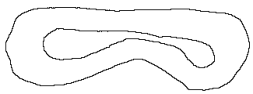
\includegraphics[interpolate=true,width=2.530000in,height=0.940000in]{contents/chapt7/figs/model/front_cornering_stiffness_path-img1.png}}%
\end{pgfscope}%
\begin{pgfscope}%
\pgfpathrectangle{\pgfqpoint{2.825000in}{0.508846in}}{\pgfqpoint{2.525000in}{0.932308in}}%
\pgfusepath{clip}%
\pgfsetrectcap%
\pgfsetroundjoin%
\pgfsetlinewidth{1.505625pt}%
\definecolor{currentstroke}{rgb}{0.121569,0.466667,0.705882}%
\pgfsetstrokecolor{currentstroke}%
\pgfsetstrokeopacity{0.700000}%
\pgfsetdash{}{0pt}%
\pgfpathmoveto{\pgfqpoint{4.378846in}{1.208077in}}%
\pgfpathlineto{\pgfqpoint{4.319453in}{1.208984in}}%
\pgfpathlineto{\pgfqpoint{4.272437in}{1.211917in}}%
\pgfpathlineto{\pgfqpoint{4.219246in}{1.217712in}}%
\pgfpathlineto{\pgfqpoint{4.134310in}{1.229708in}}%
\pgfpathlineto{\pgfqpoint{4.064742in}{1.238950in}}%
\pgfpathlineto{\pgfqpoint{4.018146in}{1.243160in}}%
\pgfpathlineto{\pgfqpoint{3.971404in}{1.245139in}}%
\pgfpathlineto{\pgfqpoint{3.924618in}{1.244952in}}%
\pgfpathlineto{\pgfqpoint{3.760912in}{1.241827in}}%
\pgfpathlineto{\pgfqpoint{3.706382in}{1.244250in}}%
\pgfpathlineto{\pgfqpoint{3.542958in}{1.254190in}}%
\pgfpathlineto{\pgfqpoint{3.503988in}{1.253121in}}%
\pgfpathlineto{\pgfqpoint{3.472922in}{1.250353in}}%
\pgfpathlineto{\pgfqpoint{3.434386in}{1.244458in}}%
\pgfpathlineto{\pgfqpoint{3.396275in}{1.236247in}}%
\pgfpathlineto{\pgfqpoint{3.358709in}{1.225820in}}%
\pgfpathlineto{\pgfqpoint{3.321797in}{1.213277in}}%
\pgfpathlineto{\pgfqpoint{3.285696in}{1.198561in}}%
\pgfpathlineto{\pgfqpoint{3.257592in}{1.185037in}}%
\pgfpathlineto{\pgfqpoint{3.230502in}{1.169589in}}%
\pgfpathlineto{\pgfqpoint{3.204811in}{1.151917in}}%
\pgfpathlineto{\pgfqpoint{3.186806in}{1.136990in}}%
\pgfpathlineto{\pgfqpoint{3.170163in}{1.120557in}}%
\pgfpathlineto{\pgfqpoint{3.155054in}{1.102706in}}%
\pgfpathlineto{\pgfqpoint{3.141785in}{1.083450in}}%
\pgfpathlineto{\pgfqpoint{3.130588in}{1.062920in}}%
\pgfpathlineto{\pgfqpoint{3.121727in}{1.041281in}}%
\pgfpathlineto{\pgfqpoint{3.115391in}{1.018773in}}%
\pgfpathlineto{\pgfqpoint{3.111726in}{0.995680in}}%
\pgfpathlineto{\pgfqpoint{3.110691in}{0.972318in}}%
\pgfpathlineto{\pgfqpoint{3.112198in}{0.948982in}}%
\pgfpathlineto{\pgfqpoint{3.116208in}{0.925945in}}%
\pgfpathlineto{\pgfqpoint{3.122695in}{0.903479in}}%
\pgfpathlineto{\pgfqpoint{3.131591in}{0.881853in}}%
\pgfpathlineto{\pgfqpoint{3.142823in}{0.861344in}}%
\pgfpathlineto{\pgfqpoint{3.156295in}{0.842230in}}%
\pgfpathlineto{\pgfqpoint{3.171814in}{0.824739in}}%
\pgfpathlineto{\pgfqpoint{3.189209in}{0.809112in}}%
\pgfpathlineto{\pgfqpoint{3.208277in}{0.795578in}}%
\pgfpathlineto{\pgfqpoint{3.228765in}{0.784308in}}%
\pgfpathlineto{\pgfqpoint{3.250375in}{0.775373in}}%
\pgfpathlineto{\pgfqpoint{3.272830in}{0.768846in}}%
\pgfpathlineto{\pgfqpoint{3.295840in}{0.764668in}}%
\pgfpathlineto{\pgfqpoint{3.319136in}{0.762586in}}%
\pgfpathlineto{\pgfqpoint{3.350320in}{0.762396in}}%
\pgfpathlineto{\pgfqpoint{3.381439in}{0.764470in}}%
\pgfpathlineto{\pgfqpoint{3.420107in}{0.769430in}}%
\pgfpathlineto{\pgfqpoint{3.473783in}{0.779344in}}%
\pgfpathlineto{\pgfqpoint{3.565240in}{0.799147in}}%
\pgfpathlineto{\pgfqpoint{3.641578in}{0.815056in}}%
\pgfpathlineto{\pgfqpoint{3.695426in}{0.823987in}}%
\pgfpathlineto{\pgfqpoint{3.757317in}{0.831798in}}%
\pgfpathlineto{\pgfqpoint{3.881169in}{0.846851in}}%
\pgfpathlineto{\pgfqpoint{4.074090in}{0.874816in}}%
\pgfpathlineto{\pgfqpoint{4.120701in}{0.878849in}}%
\pgfpathlineto{\pgfqpoint{4.159655in}{0.880468in}}%
\pgfpathlineto{\pgfqpoint{4.198638in}{0.880050in}}%
\pgfpathlineto{\pgfqpoint{4.237528in}{0.877328in}}%
\pgfpathlineto{\pgfqpoint{4.276163in}{0.872124in}}%
\pgfpathlineto{\pgfqpoint{4.314359in}{0.864327in}}%
\pgfpathlineto{\pgfqpoint{4.351969in}{0.854064in}}%
\pgfpathlineto{\pgfqpoint{4.396295in}{0.839103in}}%
\pgfpathlineto{\pgfqpoint{4.447093in}{0.819130in}}%
\pgfpathlineto{\pgfqpoint{4.504207in}{0.794042in}}%
\pgfpathlineto{\pgfqpoint{4.681165in}{0.712885in}}%
\pgfpathlineto{\pgfqpoint{4.716977in}{0.698954in}}%
\pgfpathlineto{\pgfqpoint{4.746080in}{0.689780in}}%
\pgfpathlineto{\pgfqpoint{4.768228in}{0.684559in}}%
\pgfpathlineto{\pgfqpoint{4.790600in}{0.681101in}}%
\pgfpathlineto{\pgfqpoint{4.813040in}{0.679574in}}%
\pgfpathlineto{\pgfqpoint{4.835377in}{0.679967in}}%
\pgfpathlineto{\pgfqpoint{4.857435in}{0.682384in}}%
\pgfpathlineto{\pgfqpoint{4.879029in}{0.686795in}}%
\pgfpathlineto{\pgfqpoint{4.899981in}{0.693136in}}%
\pgfpathlineto{\pgfqpoint{4.920134in}{0.701288in}}%
\pgfpathlineto{\pgfqpoint{4.939641in}{0.711290in}}%
\pgfpathlineto{\pgfqpoint{4.959020in}{0.723239in}}%
\pgfpathlineto{\pgfqpoint{4.984106in}{0.741622in}}%
\pgfpathlineto{\pgfqpoint{5.001738in}{0.756898in}}%
\pgfpathlineto{\pgfqpoint{5.018155in}{0.773471in}}%
\pgfpathlineto{\pgfqpoint{5.033142in}{0.791347in}}%
\pgfpathlineto{\pgfqpoint{5.046428in}{0.810518in}}%
\pgfpathlineto{\pgfqpoint{5.057838in}{0.830863in}}%
\pgfpathlineto{\pgfqpoint{5.067269in}{0.852196in}}%
\pgfpathlineto{\pgfqpoint{5.074604in}{0.874338in}}%
\pgfpathlineto{\pgfqpoint{5.079772in}{0.897084in}}%
\pgfpathlineto{\pgfqpoint{5.082673in}{0.920227in}}%
\pgfpathlineto{\pgfqpoint{5.083270in}{0.943544in}}%
\pgfpathlineto{\pgfqpoint{5.081474in}{0.966798in}}%
\pgfpathlineto{\pgfqpoint{5.077399in}{0.989765in}}%
\pgfpathlineto{\pgfqpoint{5.071119in}{1.012228in}}%
\pgfpathlineto{\pgfqpoint{5.062682in}{1.033974in}}%
\pgfpathlineto{\pgfqpoint{5.052125in}{1.054773in}}%
\pgfpathlineto{\pgfqpoint{5.039548in}{1.074415in}}%
\pgfpathlineto{\pgfqpoint{5.025014in}{1.092657in}}%
\pgfpathlineto{\pgfqpoint{5.008667in}{1.109294in}}%
\pgfpathlineto{\pgfqpoint{4.990808in}{1.124300in}}%
\pgfpathlineto{\pgfqpoint{4.971722in}{1.137712in}}%
\pgfpathlineto{\pgfqpoint{4.951590in}{1.149496in}}%
\pgfpathlineto{\pgfqpoint{4.930617in}{1.159712in}}%
\pgfpathlineto{\pgfqpoint{4.901639in}{1.171008in}}%
\pgfpathlineto{\pgfqpoint{4.871849in}{1.179954in}}%
\pgfpathlineto{\pgfqpoint{4.833972in}{1.188745in}}%
\pgfpathlineto{\pgfqpoint{4.788052in}{1.197035in}}%
\pgfpathlineto{\pgfqpoint{4.718750in}{1.206877in}}%
\pgfpathlineto{\pgfqpoint{4.664606in}{1.212554in}}%
\pgfpathlineto{\pgfqpoint{4.610269in}{1.215881in}}%
\pgfpathlineto{\pgfqpoint{4.548060in}{1.217062in}}%
\pgfpathlineto{\pgfqpoint{4.454754in}{1.219108in}}%
\pgfpathlineto{\pgfqpoint{4.439215in}{1.219826in}}%
\pgfpathlineto{\pgfqpoint{4.439215in}{1.219826in}}%
\pgfusepath{stroke}%
\end{pgfscope}%
\begin{pgfscope}%
\pgfpathrectangle{\pgfqpoint{2.825000in}{0.508846in}}{\pgfqpoint{2.525000in}{0.932308in}}%
\pgfusepath{clip}%
\pgfsetrectcap%
\pgfsetroundjoin%
\pgfsetlinewidth{1.505625pt}%
\definecolor{currentstroke}{rgb}{1.000000,0.498039,0.054902}%
\pgfsetstrokecolor{currentstroke}%
\pgfsetstrokeopacity{0.700000}%
\pgfsetdash{}{0pt}%
\pgfpathmoveto{\pgfqpoint{4.378846in}{1.208077in}}%
\pgfpathlineto{\pgfqpoint{4.319456in}{1.209082in}}%
\pgfpathlineto{\pgfqpoint{4.272459in}{1.212304in}}%
\pgfpathlineto{\pgfqpoint{4.219317in}{1.218429in}}%
\pgfpathlineto{\pgfqpoint{4.142196in}{1.229742in}}%
\pgfpathlineto{\pgfqpoint{4.057300in}{1.241731in}}%
\pgfpathlineto{\pgfqpoint{4.002988in}{1.246918in}}%
\pgfpathlineto{\pgfqpoint{3.956278in}{1.249174in}}%
\pgfpathlineto{\pgfqpoint{3.901718in}{1.249239in}}%
\pgfpathlineto{\pgfqpoint{3.714692in}{1.246755in}}%
\pgfpathlineto{\pgfqpoint{3.652423in}{1.250049in}}%
\pgfpathlineto{\pgfqpoint{3.559056in}{1.255486in}}%
\pgfpathlineto{\pgfqpoint{3.520090in}{1.255110in}}%
\pgfpathlineto{\pgfqpoint{3.488995in}{1.252871in}}%
\pgfpathlineto{\pgfqpoint{3.458099in}{1.248708in}}%
\pgfpathlineto{\pgfqpoint{3.419846in}{1.241279in}}%
\pgfpathlineto{\pgfqpoint{3.382055in}{1.231762in}}%
\pgfpathlineto{\pgfqpoint{3.337376in}{1.217959in}}%
\pgfpathlineto{\pgfqpoint{3.300812in}{1.204477in}}%
\pgfpathlineto{\pgfqpoint{3.264917in}{1.189304in}}%
\pgfpathlineto{\pgfqpoint{3.236949in}{1.175532in}}%
\pgfpathlineto{\pgfqpoint{3.209993in}{1.159878in}}%
\pgfpathlineto{\pgfqpoint{3.190732in}{1.146625in}}%
\pgfpathlineto{\pgfqpoint{3.172576in}{1.131897in}}%
\pgfpathlineto{\pgfqpoint{3.155698in}{1.115722in}}%
\pgfpathlineto{\pgfqpoint{3.140357in}{1.098083in}}%
\pgfpathlineto{\pgfqpoint{3.126792in}{1.079046in}}%
\pgfpathlineto{\pgfqpoint{3.115322in}{1.058679in}}%
\pgfpathlineto{\pgfqpoint{3.106162in}{1.037176in}}%
\pgfpathlineto{\pgfqpoint{3.099567in}{1.014753in}}%
\pgfpathlineto{\pgfqpoint{3.095702in}{0.991703in}}%
\pgfpathlineto{\pgfqpoint{3.094493in}{0.968360in}}%
\pgfpathlineto{\pgfqpoint{3.095792in}{0.945022in}}%
\pgfpathlineto{\pgfqpoint{3.099570in}{0.921954in}}%
\pgfpathlineto{\pgfqpoint{3.105763in}{0.899415in}}%
\pgfpathlineto{\pgfqpoint{3.114258in}{0.877638in}}%
\pgfpathlineto{\pgfqpoint{3.124988in}{0.856871in}}%
\pgfpathlineto{\pgfqpoint{3.137784in}{0.837308in}}%
\pgfpathlineto{\pgfqpoint{3.152450in}{0.819105in}}%
\pgfpathlineto{\pgfqpoint{3.168851in}{0.802450in}}%
\pgfpathlineto{\pgfqpoint{3.186869in}{0.787558in}}%
\pgfpathlineto{\pgfqpoint{3.206343in}{0.774630in}}%
\pgfpathlineto{\pgfqpoint{3.227073in}{0.763829in}}%
\pgfpathlineto{\pgfqpoint{3.248836in}{0.755302in}}%
\pgfpathlineto{\pgfqpoint{3.271362in}{0.749054in}}%
\pgfpathlineto{\pgfqpoint{3.294369in}{0.744906in}}%
\pgfpathlineto{\pgfqpoint{3.325415in}{0.742136in}}%
\pgfpathlineto{\pgfqpoint{3.356587in}{0.741859in}}%
\pgfpathlineto{\pgfqpoint{3.395488in}{0.744145in}}%
\pgfpathlineto{\pgfqpoint{3.441958in}{0.749384in}}%
\pgfpathlineto{\pgfqpoint{3.495854in}{0.757868in}}%
\pgfpathlineto{\pgfqpoint{3.549307in}{0.768793in}}%
\pgfpathlineto{\pgfqpoint{3.746942in}{0.813547in}}%
\pgfpathlineto{\pgfqpoint{3.900213in}{0.842030in}}%
\pgfpathlineto{\pgfqpoint{4.061450in}{0.870245in}}%
\pgfpathlineto{\pgfqpoint{4.115532in}{0.877451in}}%
\pgfpathlineto{\pgfqpoint{4.162126in}{0.881423in}}%
\pgfpathlineto{\pgfqpoint{4.201075in}{0.882683in}}%
\pgfpathlineto{\pgfqpoint{4.240032in}{0.881748in}}%
\pgfpathlineto{\pgfqpoint{4.278850in}{0.878330in}}%
\pgfpathlineto{\pgfqpoint{4.317345in}{0.872288in}}%
\pgfpathlineto{\pgfqpoint{4.355402in}{0.863905in}}%
\pgfpathlineto{\pgfqpoint{4.400456in}{0.851377in}}%
\pgfpathlineto{\pgfqpoint{4.444787in}{0.836490in}}%
\pgfpathlineto{\pgfqpoint{4.488339in}{0.819455in}}%
\pgfpathlineto{\pgfqpoint{4.552642in}{0.791417in}}%
\pgfpathlineto{\pgfqpoint{4.644426in}{0.748477in}}%
\pgfpathlineto{\pgfqpoint{4.708089in}{0.719017in}}%
\pgfpathlineto{\pgfqpoint{4.744351in}{0.704753in}}%
\pgfpathlineto{\pgfqpoint{4.773977in}{0.695671in}}%
\pgfpathlineto{\pgfqpoint{4.796475in}{0.690664in}}%
\pgfpathlineto{\pgfqpoint{4.819143in}{0.687554in}}%
\pgfpathlineto{\pgfqpoint{4.841835in}{0.686548in}}%
\pgfpathlineto{\pgfqpoint{4.864348in}{0.687783in}}%
\pgfpathlineto{\pgfqpoint{4.886455in}{0.691272in}}%
\pgfpathlineto{\pgfqpoint{4.908261in}{0.697112in}}%
\pgfpathlineto{\pgfqpoint{4.930204in}{0.705204in}}%
\pgfpathlineto{\pgfqpoint{4.958597in}{0.718413in}}%
\pgfpathlineto{\pgfqpoint{4.985620in}{0.734237in}}%
\pgfpathlineto{\pgfqpoint{5.004792in}{0.747807in}}%
\pgfpathlineto{\pgfqpoint{5.022808in}{0.762877in}}%
\pgfpathlineto{\pgfqpoint{5.039434in}{0.779467in}}%
\pgfpathlineto{\pgfqpoint{5.054521in}{0.797468in}}%
\pgfpathlineto{\pgfqpoint{5.067962in}{0.816730in}}%
\pgfpathlineto{\pgfqpoint{5.079604in}{0.837128in}}%
\pgfpathlineto{\pgfqpoint{5.089282in}{0.858528in}}%
\pgfpathlineto{\pgfqpoint{5.096862in}{0.880757in}}%
\pgfpathlineto{\pgfqpoint{5.102214in}{0.903625in}}%
\pgfpathlineto{\pgfqpoint{5.105224in}{0.926917in}}%
\pgfpathlineto{\pgfqpoint{5.106021in}{0.950390in}}%
\pgfpathlineto{\pgfqpoint{5.104688in}{0.973840in}}%
\pgfpathlineto{\pgfqpoint{5.101166in}{0.997061in}}%
\pgfpathlineto{\pgfqpoint{5.095453in}{1.019842in}}%
\pgfpathlineto{\pgfqpoint{5.087548in}{1.041957in}}%
\pgfpathlineto{\pgfqpoint{5.077431in}{1.063151in}}%
\pgfpathlineto{\pgfqpoint{5.065235in}{1.083222in}}%
\pgfpathlineto{\pgfqpoint{5.051238in}{1.102083in}}%
\pgfpathlineto{\pgfqpoint{5.035732in}{1.119727in}}%
\pgfpathlineto{\pgfqpoint{5.018933in}{1.136145in}}%
\pgfpathlineto{\pgfqpoint{4.994857in}{1.156172in}}%
\pgfpathlineto{\pgfqpoint{4.969196in}{1.174125in}}%
\pgfpathlineto{\pgfqpoint{4.942226in}{1.190046in}}%
\pgfpathlineto{\pgfqpoint{4.914065in}{1.203747in}}%
\pgfpathlineto{\pgfqpoint{4.884854in}{1.215037in}}%
\pgfpathlineto{\pgfqpoint{4.854769in}{1.223732in}}%
\pgfpathlineto{\pgfqpoint{4.824038in}{1.229762in}}%
\pgfpathlineto{\pgfqpoint{4.792921in}{1.233316in}}%
\pgfpathlineto{\pgfqpoint{4.753819in}{1.235305in}}%
\pgfpathlineto{\pgfqpoint{4.699002in}{1.235548in}}%
\pgfpathlineto{\pgfqpoint{4.628549in}{1.233628in}}%
\pgfpathlineto{\pgfqpoint{4.573840in}{1.230195in}}%
\pgfpathlineto{\pgfqpoint{4.519300in}{1.224686in}}%
\pgfpathlineto{\pgfqpoint{4.433670in}{1.215387in}}%
\pgfpathlineto{\pgfqpoint{4.402372in}{1.214155in}}%
\pgfpathlineto{\pgfqpoint{4.378885in}{1.214587in}}%
\pgfpathlineto{\pgfqpoint{4.378885in}{1.214587in}}%
\pgfusepath{stroke}%
\end{pgfscope}%
\begin{pgfscope}%
\definecolor{textcolor}{rgb}{0.000000,0.000000,0.000000}%
\pgfsetstrokecolor{textcolor}%
\pgfsetfillcolor{textcolor}%
\pgftext[x=4.087500in,y=1.524487in,,base]{\color{textcolor}\rmfamily\fontsize{12.000000}{14.400000}\selectfont Steering and velocity controllers}%
\end{pgfscope}%
\begin{pgfscope}%
\pgfsetbuttcap%
\pgfsetmiterjoin%
\definecolor{currentfill}{rgb}{1.000000,1.000000,1.000000}%
\pgfsetfillcolor{currentfill}%
\pgfsetfillopacity{0.800000}%
\pgfsetlinewidth{1.003750pt}%
\definecolor{currentstroke}{rgb}{0.800000,0.800000,0.800000}%
\pgfsetstrokecolor{currentstroke}%
\pgfsetstrokeopacity{0.800000}%
\pgfsetdash{}{0pt}%
\pgfpathmoveto{\pgfqpoint{0.937900in}{0.069444in}}%
\pgfpathlineto{\pgfqpoint{4.562100in}{0.069444in}}%
\pgfpathquadraticcurveto{\pgfqpoint{4.589878in}{0.069444in}}{\pgfqpoint{4.589878in}{0.097222in}}%
\pgfpathlineto{\pgfqpoint{4.589878in}{0.444675in}}%
\pgfpathquadraticcurveto{\pgfqpoint{4.589878in}{0.472452in}}{\pgfqpoint{4.562100in}{0.472452in}}%
\pgfpathlineto{\pgfqpoint{0.937900in}{0.472452in}}%
\pgfpathquadraticcurveto{\pgfqpoint{0.910122in}{0.472452in}}{\pgfqpoint{0.910122in}{0.444675in}}%
\pgfpathlineto{\pgfqpoint{0.910122in}{0.097222in}}%
\pgfpathquadraticcurveto{\pgfqpoint{0.910122in}{0.069444in}}{\pgfqpoint{0.937900in}{0.069444in}}%
\pgfpathlineto{\pgfqpoint{0.937900in}{0.069444in}}%
\pgfpathclose%
\pgfusepath{stroke,fill}%
\end{pgfscope}%
\begin{pgfscope}%
\pgfsetrectcap%
\pgfsetroundjoin%
\pgfsetlinewidth{1.505625pt}%
\definecolor{currentstroke}{rgb}{0.121569,0.466667,0.705882}%
\pgfsetstrokecolor{currentstroke}%
\pgfsetstrokeopacity{0.700000}%
\pgfsetdash{}{0pt}%
\pgfpathmoveto{\pgfqpoint{0.965678in}{0.266798in}}%
\pgfpathlineto{\pgfqpoint{1.104567in}{0.266798in}}%
\pgfpathlineto{\pgfqpoint{1.243456in}{0.266798in}}%
\pgfusepath{stroke}%
\end{pgfscope}%
\begin{pgfscope}%
\definecolor{textcolor}{rgb}{0.000000,0.000000,0.000000}%
\pgfsetstrokecolor{textcolor}%
\pgfsetfillcolor{textcolor}%
\pgftext[x=1.354567in,y=0.218187in,left,base]{\color{textcolor}\rmfamily\fontsize{10.000000}{12.000000}\selectfont No model error}%
\end{pgfscope}%
\begin{pgfscope}%
\pgfsetrectcap%
\pgfsetroundjoin%
\pgfsetlinewidth{1.505625pt}%
\definecolor{currentstroke}{rgb}{1.000000,0.498039,0.054902}%
\pgfsetstrokecolor{currentstroke}%
\pgfsetstrokeopacity{0.700000}%
\pgfsetdash{}{0pt}%
\pgfpathmoveto{\pgfqpoint{2.721619in}{0.266798in}}%
\pgfpathlineto{\pgfqpoint{2.860508in}{0.266798in}}%
\pgfpathlineto{\pgfqpoint{2.999396in}{0.266798in}}%
\pgfusepath{stroke}%
\end{pgfscope}%
\begin{pgfscope}%
\definecolor{textcolor}{rgb}{0.000000,0.000000,0.000000}%
\pgfsetstrokecolor{textcolor}%
\pgfsetfillcolor{textcolor}%
\pgftext[x=3.110507in, y=0.311374in, left, base]{\color{textcolor}\rmfamily\fontsize{10.000000}{12.000000}\selectfont Decreased front tire }%
\end{pgfscope}%
\begin{pgfscope}%
\definecolor{textcolor}{rgb}{0.000000,0.000000,0.000000}%
\pgfsetstrokecolor{textcolor}%
\pgfsetfillcolor{textcolor}%
\pgftext[x=3.110507in, y=0.155856in, left, base]{\color{textcolor}\rmfamily\fontsize{10.000000}{12.000000}\selectfont cornering stiffness}%
\end{pgfscope}%
\end{pgfpicture}%
\makeatother%
\endgroup%

    \caption[Paths taken by agents with no model error, and with a decreased tire front tire stiffness coefficient]{Paths taken by agents with no model error, and with a decreased tire front tire stiffness coefficient.}
    \label{fig:front_cornering_stiffness_-_paths}
\end{figure}

\textbf{Rear tire cornering stiffness:}
We then examined the performance of the agents under test conditions where the rear tire stiffness was modified.
The end-to-end agents experience a large decrease in successful laps under conditions where the rear tire stiffness is decreased.
The reason for this is clear when viewing Figure \ref{fig:rear_cornering_stiffness_-_paths}, which shows the paths and vehicle slip angle of end-to-end and partial end-to-end agents when the rear tire stiffness is decreased by $15\%$.
We observe large oscillations in vehicle slip angle, which indicates slaloming.
This happens because smaller rear tire cornering stiffnesses causes the rear of the car to slip more for a given lateral force.

However, our partial end-to-end agent performs much better than the end-to-end agent when the rear tire stiffness is decreased.
This is not only shown by the fact that the percentage successful laps remains constant regardless of the value of rear tire cornering stiffness coefficient, but also by the behaviour of the agent.
Figure \ref{fig:rear_cornering_stiffness_-_paths} shows that the partial end-to-end agent follows the same path as it would have without the modelling error.
Although the decreased rear tire cornering stiffness does result in larger vehicle slip angles, the vehicle does not slalom.

Interestingly, increasing the rear tire cornering stiffness causes the agents to go wide around the corners, which is similar to decreasing front tire cornering stiffness.
However, as before, the effect of increasing rear tire cornering stiffness is far more pronounced on the end-to-end agents than on the partial end-to-end agents with steering and velocity control.

\begin{figure}[htb!]
    \centering
    %% Creator: Matplotlib, PGF backend
%%
%% To include the figure in your LaTeX document, write
%%   \input{<filename>.pgf}
%%
%% Make sure the required packages are loaded in your preamble
%%   \usepackage{pgf}
%%
%% Also ensure that all the required font packages are loaded; for instance,
%% the lmodern package is sometimes necessary when using math font.
%%   \usepackage{lmodern}
%%
%% Figures using additional raster images can only be included by \input if
%% they are in the same directory as the main LaTeX file. For loading figures
%% from other directories you can use the `import` package
%%   \usepackage{import}
%%
%% and then include the figures with
%%   \import{<path to file>}{<filename>.pgf}
%%
%% Matplotlib used the following preamble
%%   \usepackage{fontspec}
%%   \setmainfont{DejaVuSerif.ttf}[Path=\detokenize{/home/andrew/anaconda3/envs/auto_car_env/lib/python3.9/site-packages/matplotlib/mpl-data/fonts/ttf/}]
%%   \setsansfont{DejaVuSans.ttf}[Path=\detokenize{/home/andrew/anaconda3/envs/auto_car_env/lib/python3.9/site-packages/matplotlib/mpl-data/fonts/ttf/}]
%%   \setmonofont{DejaVuSansMono.ttf}[Path=\detokenize{/home/andrew/anaconda3/envs/auto_car_env/lib/python3.9/site-packages/matplotlib/mpl-data/fonts/ttf/}]
%%
\begingroup%
\makeatletter%
\begin{pgfpicture}%
\pgfpathrectangle{\pgfpointorigin}{\pgfqpoint{5.500000in}{3.000000in}}%
\pgfusepath{use as bounding box, clip}%
\begin{pgfscope}%
\pgfsetbuttcap%
\pgfsetmiterjoin%
\definecolor{currentfill}{rgb}{1.000000,1.000000,1.000000}%
\pgfsetfillcolor{currentfill}%
\pgfsetlinewidth{0.000000pt}%
\definecolor{currentstroke}{rgb}{1.000000,1.000000,1.000000}%
\pgfsetstrokecolor{currentstroke}%
\pgfsetdash{}{0pt}%
\pgfpathmoveto{\pgfqpoint{0.000000in}{0.000000in}}%
\pgfpathlineto{\pgfqpoint{5.500000in}{0.000000in}}%
\pgfpathlineto{\pgfqpoint{5.500000in}{3.000000in}}%
\pgfpathlineto{\pgfqpoint{0.000000in}{3.000000in}}%
\pgfpathlineto{\pgfqpoint{0.000000in}{0.000000in}}%
\pgfpathclose%
\pgfusepath{fill}%
\end{pgfscope}%
\begin{pgfscope}%
\pgfpathrectangle{\pgfqpoint{0.892417in}{1.952323in}}{\pgfqpoint{2.077630in}{0.767125in}}%
\pgfusepath{clip}%
\pgfsys@transformshift{0.892417in}{1.952323in}%
\pgftext[left,bottom]{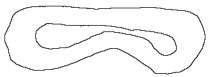
\includegraphics[interpolate=true,width=2.080000in,height=0.770000in]{contents/chapt7/figs/model/rear_c_s_decrease-img0.png}}%
\end{pgfscope}%
\begin{pgfscope}%
\pgfpathrectangle{\pgfqpoint{0.892417in}{1.952323in}}{\pgfqpoint{2.077630in}{0.767125in}}%
\pgfusepath{clip}%
\pgfsetbuttcap%
\pgfsetroundjoin%
\pgfsetlinewidth{1.505625pt}%
\definecolor{currentstroke}{rgb}{1.000000,0.000000,0.000000}%
\pgfsetstrokecolor{currentstroke}%
\pgfsetdash{{1.500000pt}{2.475000pt}}{0.000000pt}%
\pgfpathmoveto{\pgfqpoint{2.166417in}{2.403986in}}%
\pgfpathlineto{\pgfqpoint{2.166417in}{2.659695in}}%
\pgfusepath{stroke}%
\end{pgfscope}%
\begin{pgfscope}%
\pgfpathrectangle{\pgfqpoint{0.892417in}{1.952323in}}{\pgfqpoint{2.077630in}{0.767125in}}%
\pgfusepath{clip}%
\pgfsetrectcap%
\pgfsetroundjoin%
\pgfsetlinewidth{1.505625pt}%
\definecolor{currentstroke}{rgb}{0.121569,0.466667,0.705882}%
\pgfsetstrokecolor{currentstroke}%
\pgfsetstrokeopacity{0.700000}%
\pgfsetdash{}{0pt}%
\pgfpathmoveto{\pgfqpoint{2.170958in}{2.527666in}}%
\pgfpathlineto{\pgfqpoint{2.113024in}{2.528641in}}%
\pgfpathlineto{\pgfqpoint{2.056024in}{2.531921in}}%
\pgfpathlineto{\pgfqpoint{1.967814in}{2.539494in}}%
\pgfpathlineto{\pgfqpoint{1.885863in}{2.546283in}}%
\pgfpathlineto{\pgfqpoint{1.828236in}{2.548809in}}%
\pgfpathlineto{\pgfqpoint{1.738509in}{2.549937in}}%
\pgfpathlineto{\pgfqpoint{1.559044in}{2.550524in}}%
\pgfpathlineto{\pgfqpoint{1.501400in}{2.548394in}}%
\pgfpathlineto{\pgfqpoint{1.450282in}{2.544402in}}%
\pgfpathlineto{\pgfqpoint{1.399396in}{2.538113in}}%
\pgfpathlineto{\pgfqpoint{1.348864in}{2.529429in}}%
\pgfpathlineto{\pgfqpoint{1.305093in}{2.519603in}}%
\pgfpathlineto{\pgfqpoint{1.280549in}{2.512210in}}%
\pgfpathlineto{\pgfqpoint{1.256697in}{2.502829in}}%
\pgfpathlineto{\pgfqpoint{1.233920in}{2.491085in}}%
\pgfpathlineto{\pgfqpoint{1.217836in}{2.480558in}}%
\pgfpathlineto{\pgfqpoint{1.202900in}{2.468461in}}%
\pgfpathlineto{\pgfqpoint{1.189469in}{2.454714in}}%
\pgfpathlineto{\pgfqpoint{1.177817in}{2.439432in}}%
\pgfpathlineto{\pgfqpoint{1.168241in}{2.422771in}}%
\pgfpathlineto{\pgfqpoint{1.161001in}{2.404972in}}%
\pgfpathlineto{\pgfqpoint{1.156329in}{2.386334in}}%
\pgfpathlineto{\pgfqpoint{1.154371in}{2.367220in}}%
\pgfpathlineto{\pgfqpoint{1.155085in}{2.348016in}}%
\pgfpathlineto{\pgfqpoint{1.158228in}{2.329056in}}%
\pgfpathlineto{\pgfqpoint{1.163520in}{2.310579in}}%
\pgfpathlineto{\pgfqpoint{1.170760in}{2.292773in}}%
\pgfpathlineto{\pgfqpoint{1.179691in}{2.275750in}}%
\pgfpathlineto{\pgfqpoint{1.193848in}{2.254389in}}%
\pgfpathlineto{\pgfqpoint{1.210154in}{2.234616in}}%
\pgfpathlineto{\pgfqpoint{1.228209in}{2.216424in}}%
\pgfpathlineto{\pgfqpoint{1.247752in}{2.199839in}}%
\pgfpathlineto{\pgfqpoint{1.268564in}{2.184876in}}%
\pgfpathlineto{\pgfqpoint{1.290463in}{2.171554in}}%
\pgfpathlineto{\pgfqpoint{1.313321in}{2.159957in}}%
\pgfpathlineto{\pgfqpoint{1.337080in}{2.150341in}}%
\pgfpathlineto{\pgfqpoint{1.361594in}{2.142857in}}%
\pgfpathlineto{\pgfqpoint{1.386696in}{2.137687in}}%
\pgfpathlineto{\pgfqpoint{1.412182in}{2.134984in}}%
\pgfpathlineto{\pgfqpoint{1.437812in}{2.134707in}}%
\pgfpathlineto{\pgfqpoint{1.463375in}{2.136588in}}%
\pgfpathlineto{\pgfqpoint{1.488711in}{2.140480in}}%
\pgfpathlineto{\pgfqpoint{1.519888in}{2.147862in}}%
\pgfpathlineto{\pgfqpoint{1.550373in}{2.157727in}}%
\pgfpathlineto{\pgfqpoint{1.586100in}{2.171949in}}%
\pgfpathlineto{\pgfqpoint{1.662317in}{2.205623in}}%
\pgfpathlineto{\pgfqpoint{1.727368in}{2.232810in}}%
\pgfpathlineto{\pgfqpoint{1.793226in}{2.257981in}}%
\pgfpathlineto{\pgfqpoint{1.847765in}{2.276768in}}%
\pgfpathlineto{\pgfqpoint{1.896867in}{2.291535in}}%
\pgfpathlineto{\pgfqpoint{1.934180in}{2.300826in}}%
\pgfpathlineto{\pgfqpoint{1.965681in}{2.306698in}}%
\pgfpathlineto{\pgfqpoint{1.997504in}{2.310435in}}%
\pgfpathlineto{\pgfqpoint{2.029513in}{2.311699in}}%
\pgfpathlineto{\pgfqpoint{2.061412in}{2.310562in}}%
\pgfpathlineto{\pgfqpoint{2.093000in}{2.307195in}}%
\pgfpathlineto{\pgfqpoint{2.124149in}{2.301785in}}%
\pgfpathlineto{\pgfqpoint{2.154752in}{2.294552in}}%
\pgfpathlineto{\pgfqpoint{2.184411in}{2.285594in}}%
\pgfpathlineto{\pgfqpoint{2.212879in}{2.274875in}}%
\pgfpathlineto{\pgfqpoint{2.239990in}{2.262369in}}%
\pgfpathlineto{\pgfqpoint{2.265554in}{2.248089in}}%
\pgfpathlineto{\pgfqpoint{2.289327in}{2.232350in}}%
\pgfpathlineto{\pgfqpoint{2.311222in}{2.215428in}}%
\pgfpathlineto{\pgfqpoint{2.335005in}{2.193874in}}%
\pgfpathlineto{\pgfqpoint{2.356441in}{2.171093in}}%
\pgfpathlineto{\pgfqpoint{2.396702in}{2.126697in}}%
\pgfpathlineto{\pgfqpoint{2.417493in}{2.107204in}}%
\pgfpathlineto{\pgfqpoint{2.440604in}{2.088891in}}%
\pgfpathlineto{\pgfqpoint{2.461204in}{2.075592in}}%
\pgfpathlineto{\pgfqpoint{2.483768in}{2.064043in}}%
\pgfpathlineto{\pgfqpoint{2.501664in}{2.056962in}}%
\pgfpathlineto{\pgfqpoint{2.520137in}{2.051564in}}%
\pgfpathlineto{\pgfqpoint{2.539068in}{2.048113in}}%
\pgfpathlineto{\pgfqpoint{2.558264in}{2.046767in}}%
\pgfpathlineto{\pgfqpoint{2.577489in}{2.047593in}}%
\pgfpathlineto{\pgfqpoint{2.596486in}{2.050649in}}%
\pgfpathlineto{\pgfqpoint{2.614992in}{2.055921in}}%
\pgfpathlineto{\pgfqpoint{2.632754in}{2.063320in}}%
\pgfpathlineto{\pgfqpoint{2.649531in}{2.072743in}}%
\pgfpathlineto{\pgfqpoint{2.665094in}{2.084033in}}%
\pgfpathlineto{\pgfqpoint{2.679302in}{2.096917in}}%
\pgfpathlineto{\pgfqpoint{2.692166in}{2.111080in}}%
\pgfpathlineto{\pgfqpoint{2.703660in}{2.126317in}}%
\pgfpathlineto{\pgfqpoint{2.716870in}{2.147975in}}%
\pgfpathlineto{\pgfqpoint{2.727787in}{2.170782in}}%
\pgfpathlineto{\pgfqpoint{2.736540in}{2.194465in}}%
\pgfpathlineto{\pgfqpoint{2.743041in}{2.218907in}}%
\pgfpathlineto{\pgfqpoint{2.747261in}{2.243886in}}%
\pgfpathlineto{\pgfqpoint{2.749124in}{2.269193in}}%
\pgfpathlineto{\pgfqpoint{2.748547in}{2.294604in}}%
\pgfpathlineto{\pgfqpoint{2.745451in}{2.319964in}}%
\pgfpathlineto{\pgfqpoint{2.741287in}{2.338696in}}%
\pgfpathlineto{\pgfqpoint{2.735410in}{2.356963in}}%
\pgfpathlineto{\pgfqpoint{2.727769in}{2.374564in}}%
\pgfpathlineto{\pgfqpoint{2.718331in}{2.391269in}}%
\pgfpathlineto{\pgfqpoint{2.707094in}{2.406820in}}%
\pgfpathlineto{\pgfqpoint{2.694137in}{2.420969in}}%
\pgfpathlineto{\pgfqpoint{2.679671in}{2.433573in}}%
\pgfpathlineto{\pgfqpoint{2.664003in}{2.444652in}}%
\pgfpathlineto{\pgfqpoint{2.647369in}{2.454221in}}%
\pgfpathlineto{\pgfqpoint{2.624032in}{2.464698in}}%
\pgfpathlineto{\pgfqpoint{2.599750in}{2.472757in}}%
\pgfpathlineto{\pgfqpoint{2.574844in}{2.478621in}}%
\pgfpathlineto{\pgfqpoint{2.543255in}{2.483649in}}%
\pgfpathlineto{\pgfqpoint{2.505065in}{2.487539in}}%
\pgfpathlineto{\pgfqpoint{2.326594in}{2.502679in}}%
\pgfpathlineto{\pgfqpoint{2.231435in}{2.515098in}}%
\pgfpathlineto{\pgfqpoint{2.212298in}{2.516584in}}%
\pgfpathlineto{\pgfqpoint{2.212298in}{2.516584in}}%
\pgfusepath{stroke}%
\end{pgfscope}%
\begin{pgfscope}%
\pgfpathrectangle{\pgfqpoint{0.892417in}{1.952323in}}{\pgfqpoint{2.077630in}{0.767125in}}%
\pgfusepath{clip}%
\pgfsetrectcap%
\pgfsetroundjoin%
\pgfsetlinewidth{1.505625pt}%
\definecolor{currentstroke}{rgb}{1.000000,0.498039,0.054902}%
\pgfsetstrokecolor{currentstroke}%
\pgfsetstrokeopacity{0.700000}%
\pgfsetdash{}{0pt}%
\pgfpathmoveto{\pgfqpoint{2.170958in}{2.527666in}}%
\pgfpathlineto{\pgfqpoint{2.112834in}{2.528614in}}%
\pgfpathlineto{\pgfqpoint{2.060464in}{2.531559in}}%
\pgfpathlineto{\pgfqpoint{1.984379in}{2.538208in}}%
\pgfpathlineto{\pgfqpoint{1.871423in}{2.548566in}}%
\pgfpathlineto{\pgfqpoint{1.813453in}{2.551252in}}%
\pgfpathlineto{\pgfqpoint{1.742527in}{2.552165in}}%
\pgfpathlineto{\pgfqpoint{1.607114in}{2.551234in}}%
\pgfpathlineto{\pgfqpoint{1.529782in}{2.548587in}}%
\pgfpathlineto{\pgfqpoint{1.478345in}{2.544687in}}%
\pgfpathlineto{\pgfqpoint{1.433529in}{2.539318in}}%
\pgfpathlineto{\pgfqpoint{1.382616in}{2.531029in}}%
\pgfpathlineto{\pgfqpoint{1.325779in}{2.519308in}}%
\pgfpathlineto{\pgfqpoint{1.288250in}{2.509915in}}%
\pgfpathlineto{\pgfqpoint{1.263677in}{2.502089in}}%
\pgfpathlineto{\pgfqpoint{1.239844in}{2.492246in}}%
\pgfpathlineto{\pgfqpoint{1.222726in}{2.483247in}}%
\pgfpathlineto{\pgfqpoint{1.206549in}{2.472651in}}%
\pgfpathlineto{\pgfqpoint{1.191685in}{2.460287in}}%
\pgfpathlineto{\pgfqpoint{1.178573in}{2.446082in}}%
\pgfpathlineto{\pgfqpoint{1.167636in}{2.430144in}}%
\pgfpathlineto{\pgfqpoint{1.159293in}{2.412710in}}%
\pgfpathlineto{\pgfqpoint{1.153945in}{2.394140in}}%
\pgfpathlineto{\pgfqpoint{1.152197in}{2.381368in}}%
\pgfpathlineto{\pgfqpoint{1.151986in}{2.368479in}}%
\pgfpathlineto{\pgfqpoint{1.153329in}{2.355658in}}%
\pgfpathlineto{\pgfqpoint{1.156165in}{2.343082in}}%
\pgfpathlineto{\pgfqpoint{1.163031in}{2.325017in}}%
\pgfpathlineto{\pgfqpoint{1.172670in}{2.308262in}}%
\pgfpathlineto{\pgfqpoint{1.184597in}{2.293048in}}%
\pgfpathlineto{\pgfqpoint{1.198394in}{2.279503in}}%
\pgfpathlineto{\pgfqpoint{1.213668in}{2.267644in}}%
\pgfpathlineto{\pgfqpoint{1.229892in}{2.257464in}}%
\pgfpathlineto{\pgfqpoint{1.251916in}{2.246352in}}%
\pgfpathlineto{\pgfqpoint{1.274003in}{2.237822in}}%
\pgfpathlineto{\pgfqpoint{1.295847in}{2.231699in}}%
\pgfpathlineto{\pgfqpoint{1.317178in}{2.227745in}}%
\pgfpathlineto{\pgfqpoint{1.342432in}{2.225369in}}%
\pgfpathlineto{\pgfqpoint{1.410368in}{2.221279in}}%
\pgfpathlineto{\pgfqpoint{1.430040in}{2.216703in}}%
\pgfpathlineto{\pgfqpoint{1.456158in}{2.208245in}}%
\pgfpathlineto{\pgfqpoint{1.528539in}{2.183248in}}%
\pgfpathlineto{\pgfqpoint{1.557159in}{2.176362in}}%
\pgfpathlineto{\pgfqpoint{1.580875in}{2.172771in}}%
\pgfpathlineto{\pgfqpoint{1.605204in}{2.171324in}}%
\pgfpathlineto{\pgfqpoint{1.630090in}{2.172336in}}%
\pgfpathlineto{\pgfqpoint{1.655458in}{2.175776in}}%
\pgfpathlineto{\pgfqpoint{1.680424in}{2.181433in}}%
\pgfpathlineto{\pgfqpoint{1.704776in}{2.189326in}}%
\pgfpathlineto{\pgfqpoint{1.728290in}{2.199444in}}%
\pgfpathlineto{\pgfqpoint{1.750752in}{2.211723in}}%
\pgfpathlineto{\pgfqpoint{1.772148in}{2.225783in}}%
\pgfpathlineto{\pgfqpoint{1.802796in}{2.248930in}}%
\pgfpathlineto{\pgfqpoint{1.868122in}{2.299980in}}%
\pgfpathlineto{\pgfqpoint{1.889334in}{2.313216in}}%
\pgfpathlineto{\pgfqpoint{1.911571in}{2.323918in}}%
\pgfpathlineto{\pgfqpoint{1.928893in}{2.329830in}}%
\pgfpathlineto{\pgfqpoint{1.946625in}{2.333569in}}%
\pgfpathlineto{\pgfqpoint{1.964593in}{2.334859in}}%
\pgfpathlineto{\pgfqpoint{1.982613in}{2.333689in}}%
\pgfpathlineto{\pgfqpoint{2.000383in}{2.330233in}}%
\pgfpathlineto{\pgfqpoint{2.017700in}{2.324807in}}%
\pgfpathlineto{\pgfqpoint{2.039941in}{2.315120in}}%
\pgfpathlineto{\pgfqpoint{2.061187in}{2.303244in}}%
\pgfpathlineto{\pgfqpoint{2.086844in}{2.286191in}}%
\pgfpathlineto{\pgfqpoint{2.144751in}{2.246656in}}%
\pgfpathlineto{\pgfqpoint{2.172738in}{2.230967in}}%
\pgfpathlineto{\pgfqpoint{2.196053in}{2.220404in}}%
\pgfpathlineto{\pgfqpoint{2.219976in}{2.211644in}}%
\pgfpathlineto{\pgfqpoint{2.244390in}{2.204789in}}%
\pgfpathlineto{\pgfqpoint{2.275344in}{2.198809in}}%
\pgfpathlineto{\pgfqpoint{2.306550in}{2.195415in}}%
\pgfpathlineto{\pgfqpoint{2.350734in}{2.193459in}}%
\pgfpathlineto{\pgfqpoint{2.414493in}{2.190698in}}%
\pgfpathlineto{\pgfqpoint{2.445503in}{2.187268in}}%
\pgfpathlineto{\pgfqpoint{2.468591in}{2.182711in}}%
\pgfpathlineto{\pgfqpoint{2.489863in}{2.176147in}}%
\pgfpathlineto{\pgfqpoint{2.504375in}{2.169729in}}%
\pgfpathlineto{\pgfqpoint{2.517393in}{2.161973in}}%
\pgfpathlineto{\pgfqpoint{2.528731in}{2.152879in}}%
\pgfpathlineto{\pgfqpoint{2.538624in}{2.142137in}}%
\pgfpathlineto{\pgfqpoint{2.549862in}{2.125927in}}%
\pgfpathlineto{\pgfqpoint{2.564280in}{2.099454in}}%
\pgfpathlineto{\pgfqpoint{2.581680in}{2.068091in}}%
\pgfpathlineto{\pgfqpoint{2.592953in}{2.052463in}}%
\pgfpathlineto{\pgfqpoint{2.605210in}{2.039809in}}%
\pgfpathlineto{\pgfqpoint{2.615043in}{2.032692in}}%
\pgfpathlineto{\pgfqpoint{2.625288in}{2.027901in}}%
\pgfpathlineto{\pgfqpoint{2.636259in}{2.025619in}}%
\pgfpathlineto{\pgfqpoint{2.647470in}{2.025699in}}%
\pgfpathlineto{\pgfqpoint{2.658481in}{2.027827in}}%
\pgfpathlineto{\pgfqpoint{2.669015in}{2.031686in}}%
\pgfpathlineto{\pgfqpoint{2.681989in}{2.039115in}}%
\pgfpathlineto{\pgfqpoint{2.693438in}{2.048732in}}%
\pgfpathlineto{\pgfqpoint{2.703098in}{2.060147in}}%
\pgfpathlineto{\pgfqpoint{2.710833in}{2.073028in}}%
\pgfpathlineto{\pgfqpoint{2.718201in}{2.090582in}}%
\pgfpathlineto{\pgfqpoint{2.723258in}{2.109231in}}%
\pgfpathlineto{\pgfqpoint{2.726042in}{2.128639in}}%
\pgfpathlineto{\pgfqpoint{2.726661in}{2.148307in}}%
\pgfpathlineto{\pgfqpoint{2.724960in}{2.178899in}}%
\pgfpathlineto{\pgfqpoint{2.723554in}{2.209430in}}%
\pgfpathlineto{\pgfqpoint{2.724578in}{2.237478in}}%
\pgfpathlineto{\pgfqpoint{2.727424in}{2.292702in}}%
\pgfpathlineto{\pgfqpoint{2.725991in}{2.318118in}}%
\pgfpathlineto{\pgfqpoint{2.722466in}{2.338577in}}%
\pgfpathlineto{\pgfqpoint{2.716313in}{2.358737in}}%
\pgfpathlineto{\pgfqpoint{2.709757in}{2.373358in}}%
\pgfpathlineto{\pgfqpoint{2.701445in}{2.387267in}}%
\pgfpathlineto{\pgfqpoint{2.691381in}{2.400196in}}%
\pgfpathlineto{\pgfqpoint{2.679457in}{2.412093in}}%
\pgfpathlineto{\pgfqpoint{2.665811in}{2.422962in}}%
\pgfpathlineto{\pgfqpoint{2.645394in}{2.435935in}}%
\pgfpathlineto{\pgfqpoint{2.622827in}{2.447277in}}%
\pgfpathlineto{\pgfqpoint{2.598989in}{2.456767in}}%
\pgfpathlineto{\pgfqpoint{2.574450in}{2.464260in}}%
\pgfpathlineto{\pgfqpoint{2.543121in}{2.471129in}}%
\pgfpathlineto{\pgfqpoint{2.511372in}{2.475688in}}%
\pgfpathlineto{\pgfqpoint{2.473000in}{2.478723in}}%
\pgfpathlineto{\pgfqpoint{2.402466in}{2.481162in}}%
\pgfpathlineto{\pgfqpoint{2.351210in}{2.483840in}}%
\pgfpathlineto{\pgfqpoint{2.312913in}{2.487715in}}%
\pgfpathlineto{\pgfqpoint{2.262148in}{2.495271in}}%
\pgfpathlineto{\pgfqpoint{2.211703in}{2.504753in}}%
\pgfpathlineto{\pgfqpoint{2.211703in}{2.504753in}}%
\pgfusepath{stroke}%
\end{pgfscope}%
\begin{pgfscope}%
\pgfsetbuttcap%
\pgfsetmiterjoin%
\definecolor{currentfill}{rgb}{1.000000,1.000000,1.000000}%
\pgfsetfillcolor{currentfill}%
\pgfsetlinewidth{1.003750pt}%
\definecolor{currentstroke}{rgb}{0.000000,0.000000,0.000000}%
\pgfsetstrokecolor{currentstroke}%
\pgfsetdash{}{0pt}%
\pgfpathmoveto{\pgfqpoint{1.375655in}{2.529458in}}%
\pgfpathlineto{\pgfqpoint{1.632804in}{2.529458in}}%
\pgfpathquadraticcurveto{\pgfqpoint{1.644373in}{2.529458in}}{\pgfqpoint{1.644373in}{2.541027in}}%
\pgfpathlineto{\pgfqpoint{1.644373in}{2.652993in}}%
\pgfpathquadraticcurveto{\pgfqpoint{1.644373in}{2.664563in}}{\pgfqpoint{1.632804in}{2.664563in}}%
\pgfpathlineto{\pgfqpoint{1.375655in}{2.664563in}}%
\pgfpathquadraticcurveto{\pgfqpoint{1.364086in}{2.664563in}}{\pgfqpoint{1.364086in}{2.652993in}}%
\pgfpathlineto{\pgfqpoint{1.364086in}{2.541027in}}%
\pgfpathquadraticcurveto{\pgfqpoint{1.364086in}{2.529458in}}{\pgfqpoint{1.375655in}{2.529458in}}%
\pgfpathlineto{\pgfqpoint{1.375655in}{2.529458in}}%
\pgfpathclose%
\pgfusepath{stroke,fill}%
\end{pgfscope}%
\begin{pgfscope}%
\definecolor{textcolor}{rgb}{0.000000,0.000000,0.000000}%
\pgfsetstrokecolor{textcolor}%
\pgfsetfillcolor{textcolor}%
\pgftext[x=1.375655in,y=2.565093in,left,base]{\color{textcolor}\rmfamily\fontsize{8.330000}{9.996000}\selectfont 20\%}%
\end{pgfscope}%
\begin{pgfscope}%
\pgfsetbuttcap%
\pgfsetmiterjoin%
\definecolor{currentfill}{rgb}{1.000000,1.000000,1.000000}%
\pgfsetfillcolor{currentfill}%
\pgfsetlinewidth{1.003750pt}%
\definecolor{currentstroke}{rgb}{0.000000,0.000000,0.000000}%
\pgfsetstrokecolor{currentstroke}%
\pgfsetdash{}{0pt}%
\pgfpathmoveto{\pgfqpoint{1.373218in}{2.095962in}}%
\pgfpathlineto{\pgfqpoint{1.630367in}{2.095962in}}%
\pgfpathquadraticcurveto{\pgfqpoint{1.641936in}{2.095962in}}{\pgfqpoint{1.641936in}{2.107532in}}%
\pgfpathlineto{\pgfqpoint{1.641936in}{2.219498in}}%
\pgfpathquadraticcurveto{\pgfqpoint{1.641936in}{2.231067in}}{\pgfqpoint{1.630367in}{2.231067in}}%
\pgfpathlineto{\pgfqpoint{1.373218in}{2.231067in}}%
\pgfpathquadraticcurveto{\pgfqpoint{1.361649in}{2.231067in}}{\pgfqpoint{1.361649in}{2.219498in}}%
\pgfpathlineto{\pgfqpoint{1.361649in}{2.107532in}}%
\pgfpathquadraticcurveto{\pgfqpoint{1.361649in}{2.095962in}}{\pgfqpoint{1.373218in}{2.095962in}}%
\pgfpathlineto{\pgfqpoint{1.373218in}{2.095962in}}%
\pgfpathclose%
\pgfusepath{stroke,fill}%
\end{pgfscope}%
\begin{pgfscope}%
\definecolor{textcolor}{rgb}{0.000000,0.000000,0.000000}%
\pgfsetstrokecolor{textcolor}%
\pgfsetfillcolor{textcolor}%
\pgftext[x=1.373218in,y=2.131597in,left,base]{\color{textcolor}\rmfamily\fontsize{8.330000}{9.996000}\selectfont 40\%}%
\end{pgfscope}%
\begin{pgfscope}%
\pgfsetbuttcap%
\pgfsetmiterjoin%
\definecolor{currentfill}{rgb}{1.000000,1.000000,1.000000}%
\pgfsetfillcolor{currentfill}%
\pgfsetlinewidth{1.003750pt}%
\definecolor{currentstroke}{rgb}{0.000000,0.000000,0.000000}%
\pgfsetstrokecolor{currentstroke}%
\pgfsetdash{}{0pt}%
\pgfpathmoveto{\pgfqpoint{2.129819in}{2.263270in}}%
\pgfpathlineto{\pgfqpoint{2.386968in}{2.263270in}}%
\pgfpathquadraticcurveto{\pgfqpoint{2.398538in}{2.263270in}}{\pgfqpoint{2.398538in}{2.274839in}}%
\pgfpathlineto{\pgfqpoint{2.398538in}{2.386805in}}%
\pgfpathquadraticcurveto{\pgfqpoint{2.398538in}{2.398375in}}{\pgfqpoint{2.386968in}{2.398375in}}%
\pgfpathlineto{\pgfqpoint{2.129819in}{2.398375in}}%
\pgfpathquadraticcurveto{\pgfqpoint{2.118250in}{2.398375in}}{\pgfqpoint{2.118250in}{2.386805in}}%
\pgfpathlineto{\pgfqpoint{2.118250in}{2.274839in}}%
\pgfpathquadraticcurveto{\pgfqpoint{2.118250in}{2.263270in}}{\pgfqpoint{2.129819in}{2.263270in}}%
\pgfpathlineto{\pgfqpoint{2.129819in}{2.263270in}}%
\pgfpathclose%
\pgfusepath{stroke,fill}%
\end{pgfscope}%
\begin{pgfscope}%
\definecolor{textcolor}{rgb}{0.000000,0.000000,0.000000}%
\pgfsetstrokecolor{textcolor}%
\pgfsetfillcolor{textcolor}%
\pgftext[x=2.129819in,y=2.298905in,left,base]{\color{textcolor}\rmfamily\fontsize{8.330000}{9.996000}\selectfont 60\%}%
\end{pgfscope}%
\begin{pgfscope}%
\pgfsetbuttcap%
\pgfsetmiterjoin%
\definecolor{currentfill}{rgb}{1.000000,1.000000,1.000000}%
\pgfsetfillcolor{currentfill}%
\pgfsetlinewidth{1.003750pt}%
\definecolor{currentstroke}{rgb}{0.000000,0.000000,0.000000}%
\pgfsetstrokecolor{currentstroke}%
\pgfsetdash{}{0pt}%
\pgfpathmoveto{\pgfqpoint{2.775593in}{2.206871in}}%
\pgfpathlineto{\pgfqpoint{3.032742in}{2.206871in}}%
\pgfpathquadraticcurveto{\pgfqpoint{3.044311in}{2.206871in}}{\pgfqpoint{3.044311in}{2.218440in}}%
\pgfpathlineto{\pgfqpoint{3.044311in}{2.330406in}}%
\pgfpathquadraticcurveto{\pgfqpoint{3.044311in}{2.341975in}}{\pgfqpoint{3.032742in}{2.341975in}}%
\pgfpathlineto{\pgfqpoint{2.775593in}{2.341975in}}%
\pgfpathquadraticcurveto{\pgfqpoint{2.764024in}{2.341975in}}{\pgfqpoint{2.764024in}{2.330406in}}%
\pgfpathlineto{\pgfqpoint{2.764024in}{2.218440in}}%
\pgfpathquadraticcurveto{\pgfqpoint{2.764024in}{2.206871in}}{\pgfqpoint{2.775593in}{2.206871in}}%
\pgfpathlineto{\pgfqpoint{2.775593in}{2.206871in}}%
\pgfpathclose%
\pgfusepath{stroke,fill}%
\end{pgfscope}%
\begin{pgfscope}%
\definecolor{textcolor}{rgb}{0.000000,0.000000,0.000000}%
\pgfsetstrokecolor{textcolor}%
\pgfsetfillcolor{textcolor}%
\pgftext[x=2.775593in,y=2.242505in,left,base]{\color{textcolor}\rmfamily\fontsize{8.330000}{9.996000}\selectfont 80\%}%
\end{pgfscope}%
\begin{pgfscope}%
\definecolor{textcolor}{rgb}{0.000000,0.000000,0.000000}%
\pgfsetstrokecolor{textcolor}%
\pgfsetfillcolor{textcolor}%
\pgftext[x=1.931232in,y=2.802781in,,base]{\color{textcolor}\rmfamily\fontsize{12.000000}{14.400000}\selectfont End-to-end}%
\end{pgfscope}%
\begin{pgfscope}%
\pgfpathrectangle{\pgfqpoint{3.196208in}{1.952323in}}{\pgfqpoint{2.077630in}{0.767125in}}%
\pgfusepath{clip}%
\pgfsys@transformshift{3.196208in}{1.952323in}%
\pgftext[left,bottom]{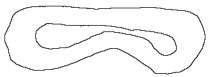
\includegraphics[interpolate=true,width=2.080000in,height=0.770000in]{contents/chapt7/figs/model/rear_c_s_decrease-img1.png}}%
\end{pgfscope}%
\begin{pgfscope}%
\pgfpathrectangle{\pgfqpoint{3.196208in}{1.952323in}}{\pgfqpoint{2.077630in}{0.767125in}}%
\pgfusepath{clip}%
\pgfsetbuttcap%
\pgfsetroundjoin%
\pgfsetlinewidth{1.505625pt}%
\definecolor{currentstroke}{rgb}{1.000000,0.000000,0.000000}%
\pgfsetstrokecolor{currentstroke}%
\pgfsetdash{{1.500000pt}{2.475000pt}}{0.000000pt}%
\pgfpathmoveto{\pgfqpoint{4.470209in}{2.403986in}}%
\pgfpathlineto{\pgfqpoint{4.470209in}{2.659695in}}%
\pgfusepath{stroke}%
\end{pgfscope}%
\begin{pgfscope}%
\pgfpathrectangle{\pgfqpoint{3.196208in}{1.952323in}}{\pgfqpoint{2.077630in}{0.767125in}}%
\pgfusepath{clip}%
\pgfsetrectcap%
\pgfsetroundjoin%
\pgfsetlinewidth{1.505625pt}%
\definecolor{currentstroke}{rgb}{0.121569,0.466667,0.705882}%
\pgfsetstrokecolor{currentstroke}%
\pgfsetstrokeopacity{0.700000}%
\pgfsetdash{}{0pt}%
\pgfpathmoveto{\pgfqpoint{4.474750in}{2.527666in}}%
\pgfpathlineto{\pgfqpoint{4.420920in}{2.528624in}}%
\pgfpathlineto{\pgfqpoint{4.372204in}{2.531842in}}%
\pgfpathlineto{\pgfqpoint{4.228184in}{2.544277in}}%
\pgfpathlineto{\pgfqpoint{4.159018in}{2.546752in}}%
\pgfpathlineto{\pgfqpoint{4.082526in}{2.547189in}}%
\pgfpathlineto{\pgfqpoint{4.025064in}{2.545304in}}%
\pgfpathlineto{\pgfqpoint{3.961237in}{2.540747in}}%
\pgfpathlineto{\pgfqpoint{3.891272in}{2.533450in}}%
\pgfpathlineto{\pgfqpoint{3.808855in}{2.522535in}}%
\pgfpathlineto{\pgfqpoint{3.726784in}{2.509442in}}%
\pgfpathlineto{\pgfqpoint{3.664179in}{2.497598in}}%
\pgfpathlineto{\pgfqpoint{3.626896in}{2.488734in}}%
\pgfpathlineto{\pgfqpoint{3.596392in}{2.479444in}}%
\pgfpathlineto{\pgfqpoint{3.572638in}{2.470221in}}%
\pgfpathlineto{\pgfqpoint{3.549666in}{2.458979in}}%
\pgfpathlineto{\pgfqpoint{3.527932in}{2.445504in}}%
\pgfpathlineto{\pgfqpoint{3.512748in}{2.433820in}}%
\pgfpathlineto{\pgfqpoint{3.498700in}{2.420742in}}%
\pgfpathlineto{\pgfqpoint{3.486028in}{2.406341in}}%
\pgfpathlineto{\pgfqpoint{3.474912in}{2.390712in}}%
\pgfpathlineto{\pgfqpoint{3.465574in}{2.373964in}}%
\pgfpathlineto{\pgfqpoint{3.458213in}{2.356265in}}%
\pgfpathlineto{\pgfqpoint{3.452968in}{2.337839in}}%
\pgfpathlineto{\pgfqpoint{3.449968in}{2.318912in}}%
\pgfpathlineto{\pgfqpoint{3.449246in}{2.299748in}}%
\pgfpathlineto{\pgfqpoint{3.450788in}{2.280632in}}%
\pgfpathlineto{\pgfqpoint{3.454575in}{2.261860in}}%
\pgfpathlineto{\pgfqpoint{3.460538in}{2.243685in}}%
\pgfpathlineto{\pgfqpoint{3.468613in}{2.226319in}}%
\pgfpathlineto{\pgfqpoint{3.478650in}{2.209999in}}%
\pgfpathlineto{\pgfqpoint{3.490477in}{2.194951in}}%
\pgfpathlineto{\pgfqpoint{3.503859in}{2.181234in}}%
\pgfpathlineto{\pgfqpoint{3.518608in}{2.168990in}}%
\pgfpathlineto{\pgfqpoint{3.534517in}{2.158302in}}%
\pgfpathlineto{\pgfqpoint{3.551417in}{2.149226in}}%
\pgfpathlineto{\pgfqpoint{3.569058in}{2.141773in}}%
\pgfpathlineto{\pgfqpoint{3.587265in}{2.135931in}}%
\pgfpathlineto{\pgfqpoint{3.612221in}{2.130600in}}%
\pgfpathlineto{\pgfqpoint{3.637594in}{2.127811in}}%
\pgfpathlineto{\pgfqpoint{3.663122in}{2.127404in}}%
\pgfpathlineto{\pgfqpoint{3.688627in}{2.129190in}}%
\pgfpathlineto{\pgfqpoint{3.713904in}{2.133002in}}%
\pgfpathlineto{\pgfqpoint{3.745014in}{2.140174in}}%
\pgfpathlineto{\pgfqpoint{3.794114in}{2.154514in}}%
\pgfpathlineto{\pgfqpoint{3.879872in}{2.180057in}}%
\pgfpathlineto{\pgfqpoint{3.991018in}{2.209322in}}%
\pgfpathlineto{\pgfqpoint{4.127074in}{2.243918in}}%
\pgfpathlineto{\pgfqpoint{4.177185in}{2.254031in}}%
\pgfpathlineto{\pgfqpoint{4.215074in}{2.259628in}}%
\pgfpathlineto{\pgfqpoint{4.253315in}{2.263074in}}%
\pgfpathlineto{\pgfqpoint{4.285277in}{2.264027in}}%
\pgfpathlineto{\pgfqpoint{4.317164in}{2.263052in}}%
\pgfpathlineto{\pgfqpoint{4.348899in}{2.260197in}}%
\pgfpathlineto{\pgfqpoint{4.380500in}{2.255369in}}%
\pgfpathlineto{\pgfqpoint{4.411791in}{2.248539in}}%
\pgfpathlineto{\pgfqpoint{4.448678in}{2.237884in}}%
\pgfpathlineto{\pgfqpoint{4.484727in}{2.224754in}}%
\pgfpathlineto{\pgfqpoint{4.574235in}{2.190172in}}%
\pgfpathlineto{\pgfqpoint{4.610868in}{2.178816in}}%
\pgfpathlineto{\pgfqpoint{4.666463in}{2.164060in}}%
\pgfpathlineto{\pgfqpoint{4.722481in}{2.151241in}}%
\pgfpathlineto{\pgfqpoint{4.766527in}{2.143525in}}%
\pgfpathlineto{\pgfqpoint{4.798272in}{2.140079in}}%
\pgfpathlineto{\pgfqpoint{4.830198in}{2.138888in}}%
\pgfpathlineto{\pgfqpoint{4.855699in}{2.139917in}}%
\pgfpathlineto{\pgfqpoint{4.880857in}{2.142989in}}%
\pgfpathlineto{\pgfqpoint{4.905622in}{2.148346in}}%
\pgfpathlineto{\pgfqpoint{4.929582in}{2.156164in}}%
\pgfpathlineto{\pgfqpoint{4.952463in}{2.166521in}}%
\pgfpathlineto{\pgfqpoint{4.968732in}{2.175969in}}%
\pgfpathlineto{\pgfqpoint{4.984137in}{2.186926in}}%
\pgfpathlineto{\pgfqpoint{4.998544in}{2.199312in}}%
\pgfpathlineto{\pgfqpoint{5.011746in}{2.213027in}}%
\pgfpathlineto{\pgfqpoint{5.023553in}{2.227971in}}%
\pgfpathlineto{\pgfqpoint{5.033827in}{2.244042in}}%
\pgfpathlineto{\pgfqpoint{5.042420in}{2.261132in}}%
\pgfpathlineto{\pgfqpoint{5.049171in}{2.279000in}}%
\pgfpathlineto{\pgfqpoint{5.053950in}{2.297458in}}%
\pgfpathlineto{\pgfqpoint{5.056652in}{2.316326in}}%
\pgfpathlineto{\pgfqpoint{5.057149in}{2.335397in}}%
\pgfpathlineto{\pgfqpoint{5.055472in}{2.354471in}}%
\pgfpathlineto{\pgfqpoint{5.051646in}{2.373238in}}%
\pgfpathlineto{\pgfqpoint{5.045727in}{2.391457in}}%
\pgfpathlineto{\pgfqpoint{5.037857in}{2.408904in}}%
\pgfpathlineto{\pgfqpoint{5.028138in}{2.425371in}}%
\pgfpathlineto{\pgfqpoint{5.016679in}{2.440724in}}%
\pgfpathlineto{\pgfqpoint{5.003689in}{2.454757in}}%
\pgfpathlineto{\pgfqpoint{4.989384in}{2.467375in}}%
\pgfpathlineto{\pgfqpoint{4.973895in}{2.478497in}}%
\pgfpathlineto{\pgfqpoint{4.957366in}{2.488072in}}%
\pgfpathlineto{\pgfqpoint{4.934169in}{2.498686in}}%
\pgfpathlineto{\pgfqpoint{4.910053in}{2.507205in}}%
\pgfpathlineto{\pgfqpoint{4.879180in}{2.515474in}}%
\pgfpathlineto{\pgfqpoint{4.841524in}{2.522758in}}%
\pgfpathlineto{\pgfqpoint{4.797220in}{2.528760in}}%
\pgfpathlineto{\pgfqpoint{4.746245in}{2.533085in}}%
\pgfpathlineto{\pgfqpoint{4.682428in}{2.536056in}}%
\pgfpathlineto{\pgfqpoint{4.522940in}{2.542655in}}%
\pgfpathlineto{\pgfqpoint{4.472124in}{2.546102in}}%
\pgfpathlineto{\pgfqpoint{4.472124in}{2.546102in}}%
\pgfusepath{stroke}%
\end{pgfscope}%
\begin{pgfscope}%
\pgfpathrectangle{\pgfqpoint{3.196208in}{1.952323in}}{\pgfqpoint{2.077630in}{0.767125in}}%
\pgfusepath{clip}%
\pgfsetrectcap%
\pgfsetroundjoin%
\pgfsetlinewidth{1.505625pt}%
\definecolor{currentstroke}{rgb}{1.000000,0.498039,0.054902}%
\pgfsetstrokecolor{currentstroke}%
\pgfsetstrokeopacity{0.700000}%
\pgfsetdash{}{0pt}%
\pgfpathmoveto{\pgfqpoint{4.474750in}{2.527666in}}%
\pgfpathlineto{\pgfqpoint{4.415854in}{2.528694in}}%
\pgfpathlineto{\pgfqpoint{4.366639in}{2.531852in}}%
\pgfpathlineto{\pgfqpoint{4.208836in}{2.544952in}}%
\pgfpathlineto{\pgfqpoint{4.145623in}{2.546887in}}%
\pgfpathlineto{\pgfqpoint{4.075358in}{2.546636in}}%
\pgfpathlineto{\pgfqpoint{4.017846in}{2.543939in}}%
\pgfpathlineto{\pgfqpoint{3.960533in}{2.538753in}}%
\pgfpathlineto{\pgfqpoint{3.903510in}{2.531281in}}%
\pgfpathlineto{\pgfqpoint{3.745416in}{2.508421in}}%
\pgfpathlineto{\pgfqpoint{3.668908in}{2.502983in}}%
\pgfpathlineto{\pgfqpoint{3.630795in}{2.499023in}}%
\pgfpathlineto{\pgfqpoint{3.599359in}{2.493458in}}%
\pgfpathlineto{\pgfqpoint{3.574689in}{2.486776in}}%
\pgfpathlineto{\pgfqpoint{3.550808in}{2.477684in}}%
\pgfpathlineto{\pgfqpoint{3.533663in}{2.469109in}}%
\pgfpathlineto{\pgfqpoint{3.517430in}{2.458910in}}%
\pgfpathlineto{\pgfqpoint{3.502360in}{2.447086in}}%
\pgfpathlineto{\pgfqpoint{3.488676in}{2.433659in}}%
\pgfpathlineto{\pgfqpoint{3.476639in}{2.418745in}}%
\pgfpathlineto{\pgfqpoint{3.466431in}{2.402513in}}%
\pgfpathlineto{\pgfqpoint{3.458251in}{2.385167in}}%
\pgfpathlineto{\pgfqpoint{3.452237in}{2.366942in}}%
\pgfpathlineto{\pgfqpoint{3.448510in}{2.348122in}}%
\pgfpathlineto{\pgfqpoint{3.447125in}{2.329001in}}%
\pgfpathlineto{\pgfqpoint{3.448123in}{2.309885in}}%
\pgfpathlineto{\pgfqpoint{3.451497in}{2.291030in}}%
\pgfpathlineto{\pgfqpoint{3.457208in}{2.272737in}}%
\pgfpathlineto{\pgfqpoint{3.465118in}{2.255270in}}%
\pgfpathlineto{\pgfqpoint{3.475069in}{2.238864in}}%
\pgfpathlineto{\pgfqpoint{3.486887in}{2.223776in}}%
\pgfpathlineto{\pgfqpoint{3.500371in}{2.210143in}}%
\pgfpathlineto{\pgfqpoint{3.515303in}{2.198083in}}%
\pgfpathlineto{\pgfqpoint{3.531419in}{2.187658in}}%
\pgfpathlineto{\pgfqpoint{3.548496in}{2.178934in}}%
\pgfpathlineto{\pgfqpoint{3.566360in}{2.171909in}}%
\pgfpathlineto{\pgfqpoint{3.584773in}{2.166521in}}%
\pgfpathlineto{\pgfqpoint{3.609904in}{2.161820in}}%
\pgfpathlineto{\pgfqpoint{3.635363in}{2.159582in}}%
\pgfpathlineto{\pgfqpoint{3.660855in}{2.159300in}}%
\pgfpathlineto{\pgfqpoint{3.692687in}{2.161175in}}%
\pgfpathlineto{\pgfqpoint{3.730709in}{2.165653in}}%
\pgfpathlineto{\pgfqpoint{3.787498in}{2.174757in}}%
\pgfpathlineto{\pgfqpoint{3.869162in}{2.190019in}}%
\pgfpathlineto{\pgfqpoint{3.950482in}{2.207237in}}%
\pgfpathlineto{\pgfqpoint{4.031274in}{2.226750in}}%
\pgfpathlineto{\pgfqpoint{4.155260in}{2.256986in}}%
\pgfpathlineto{\pgfqpoint{4.199242in}{2.264925in}}%
\pgfpathlineto{\pgfqpoint{4.230932in}{2.268682in}}%
\pgfpathlineto{\pgfqpoint{4.262830in}{2.270495in}}%
\pgfpathlineto{\pgfqpoint{4.294764in}{2.270216in}}%
\pgfpathlineto{\pgfqpoint{4.326709in}{2.267736in}}%
\pgfpathlineto{\pgfqpoint{4.358356in}{2.263058in}}%
\pgfpathlineto{\pgfqpoint{4.395864in}{2.254980in}}%
\pgfpathlineto{\pgfqpoint{4.457696in}{2.238842in}}%
\pgfpathlineto{\pgfqpoint{4.532039in}{2.219984in}}%
\pgfpathlineto{\pgfqpoint{4.600831in}{2.205338in}}%
\pgfpathlineto{\pgfqpoint{4.663295in}{2.191891in}}%
\pgfpathlineto{\pgfqpoint{4.706497in}{2.180269in}}%
\pgfpathlineto{\pgfqpoint{4.761248in}{2.162707in}}%
\pgfpathlineto{\pgfqpoint{4.804199in}{2.149972in}}%
\pgfpathlineto{\pgfqpoint{4.835463in}{2.143334in}}%
\pgfpathlineto{\pgfqpoint{4.860858in}{2.140420in}}%
\pgfpathlineto{\pgfqpoint{4.886329in}{2.140209in}}%
\pgfpathlineto{\pgfqpoint{4.905343in}{2.142075in}}%
\pgfpathlineto{\pgfqpoint{4.924044in}{2.145812in}}%
\pgfpathlineto{\pgfqpoint{4.942232in}{2.151476in}}%
\pgfpathlineto{\pgfqpoint{4.959671in}{2.159096in}}%
\pgfpathlineto{\pgfqpoint{4.976152in}{2.168642in}}%
\pgfpathlineto{\pgfqpoint{4.991422in}{2.180033in}}%
\pgfpathlineto{\pgfqpoint{5.005294in}{2.193110in}}%
\pgfpathlineto{\pgfqpoint{5.017568in}{2.207679in}}%
\pgfpathlineto{\pgfqpoint{5.028023in}{2.223581in}}%
\pgfpathlineto{\pgfqpoint{5.036532in}{2.240646in}}%
\pgfpathlineto{\pgfqpoint{5.042973in}{2.258623in}}%
\pgfpathlineto{\pgfqpoint{5.047243in}{2.277274in}}%
\pgfpathlineto{\pgfqpoint{5.049285in}{2.296313in}}%
\pgfpathlineto{\pgfqpoint{5.049055in}{2.315502in}}%
\pgfpathlineto{\pgfqpoint{5.046562in}{2.334526in}}%
\pgfpathlineto{\pgfqpoint{5.041821in}{2.353113in}}%
\pgfpathlineto{\pgfqpoint{5.034938in}{2.370993in}}%
\pgfpathlineto{\pgfqpoint{5.026022in}{2.387938in}}%
\pgfpathlineto{\pgfqpoint{5.015195in}{2.403730in}}%
\pgfpathlineto{\pgfqpoint{5.002667in}{2.418205in}}%
\pgfpathlineto{\pgfqpoint{4.988603in}{2.431236in}}%
\pgfpathlineto{\pgfqpoint{4.973267in}{2.442743in}}%
\pgfpathlineto{\pgfqpoint{4.956864in}{2.452679in}}%
\pgfpathlineto{\pgfqpoint{4.939621in}{2.461067in}}%
\pgfpathlineto{\pgfqpoint{4.915628in}{2.469887in}}%
\pgfpathlineto{\pgfqpoint{4.890927in}{2.476431in}}%
\pgfpathlineto{\pgfqpoint{4.859590in}{2.482351in}}%
\pgfpathlineto{\pgfqpoint{4.815321in}{2.488103in}}%
\pgfpathlineto{\pgfqpoint{4.688509in}{2.503308in}}%
\pgfpathlineto{\pgfqpoint{4.561890in}{2.520807in}}%
\pgfpathlineto{\pgfqpoint{4.549178in}{2.522099in}}%
\pgfpathlineto{\pgfqpoint{4.549178in}{2.522099in}}%
\pgfusepath{stroke}%
\end{pgfscope}%
\begin{pgfscope}%
\pgfsetbuttcap%
\pgfsetmiterjoin%
\definecolor{currentfill}{rgb}{1.000000,1.000000,1.000000}%
\pgfsetfillcolor{currentfill}%
\pgfsetlinewidth{1.003750pt}%
\definecolor{currentstroke}{rgb}{0.000000,0.000000,0.000000}%
\pgfsetstrokecolor{currentstroke}%
\pgfsetdash{}{0pt}%
\pgfpathmoveto{\pgfqpoint{3.679447in}{2.529458in}}%
\pgfpathlineto{\pgfqpoint{3.936596in}{2.529458in}}%
\pgfpathquadraticcurveto{\pgfqpoint{3.948165in}{2.529458in}}{\pgfqpoint{3.948165in}{2.541027in}}%
\pgfpathlineto{\pgfqpoint{3.948165in}{2.652993in}}%
\pgfpathquadraticcurveto{\pgfqpoint{3.948165in}{2.664563in}}{\pgfqpoint{3.936596in}{2.664563in}}%
\pgfpathlineto{\pgfqpoint{3.679447in}{2.664563in}}%
\pgfpathquadraticcurveto{\pgfqpoint{3.667877in}{2.664563in}}{\pgfqpoint{3.667877in}{2.652993in}}%
\pgfpathlineto{\pgfqpoint{3.667877in}{2.541027in}}%
\pgfpathquadraticcurveto{\pgfqpoint{3.667877in}{2.529458in}}{\pgfqpoint{3.679447in}{2.529458in}}%
\pgfpathlineto{\pgfqpoint{3.679447in}{2.529458in}}%
\pgfpathclose%
\pgfusepath{stroke,fill}%
\end{pgfscope}%
\begin{pgfscope}%
\definecolor{textcolor}{rgb}{0.000000,0.000000,0.000000}%
\pgfsetstrokecolor{textcolor}%
\pgfsetfillcolor{textcolor}%
\pgftext[x=3.679447in,y=2.565093in,left,base]{\color{textcolor}\rmfamily\fontsize{8.330000}{9.996000}\selectfont 20\%}%
\end{pgfscope}%
\begin{pgfscope}%
\pgfsetbuttcap%
\pgfsetmiterjoin%
\definecolor{currentfill}{rgb}{1.000000,1.000000,1.000000}%
\pgfsetfillcolor{currentfill}%
\pgfsetlinewidth{1.003750pt}%
\definecolor{currentstroke}{rgb}{0.000000,0.000000,0.000000}%
\pgfsetstrokecolor{currentstroke}%
\pgfsetdash{}{0pt}%
\pgfpathmoveto{\pgfqpoint{3.677010in}{2.095962in}}%
\pgfpathlineto{\pgfqpoint{3.934159in}{2.095962in}}%
\pgfpathquadraticcurveto{\pgfqpoint{3.945728in}{2.095962in}}{\pgfqpoint{3.945728in}{2.107532in}}%
\pgfpathlineto{\pgfqpoint{3.945728in}{2.219498in}}%
\pgfpathquadraticcurveto{\pgfqpoint{3.945728in}{2.231067in}}{\pgfqpoint{3.934159in}{2.231067in}}%
\pgfpathlineto{\pgfqpoint{3.677010in}{2.231067in}}%
\pgfpathquadraticcurveto{\pgfqpoint{3.665440in}{2.231067in}}{\pgfqpoint{3.665440in}{2.219498in}}%
\pgfpathlineto{\pgfqpoint{3.665440in}{2.107532in}}%
\pgfpathquadraticcurveto{\pgfqpoint{3.665440in}{2.095962in}}{\pgfqpoint{3.677010in}{2.095962in}}%
\pgfpathlineto{\pgfqpoint{3.677010in}{2.095962in}}%
\pgfpathclose%
\pgfusepath{stroke,fill}%
\end{pgfscope}%
\begin{pgfscope}%
\definecolor{textcolor}{rgb}{0.000000,0.000000,0.000000}%
\pgfsetstrokecolor{textcolor}%
\pgfsetfillcolor{textcolor}%
\pgftext[x=3.677010in,y=2.131597in,left,base]{\color{textcolor}\rmfamily\fontsize{8.330000}{9.996000}\selectfont 40\%}%
\end{pgfscope}%
\begin{pgfscope}%
\pgfsetbuttcap%
\pgfsetmiterjoin%
\definecolor{currentfill}{rgb}{1.000000,1.000000,1.000000}%
\pgfsetfillcolor{currentfill}%
\pgfsetlinewidth{1.003750pt}%
\definecolor{currentstroke}{rgb}{0.000000,0.000000,0.000000}%
\pgfsetstrokecolor{currentstroke}%
\pgfsetdash{}{0pt}%
\pgfpathmoveto{\pgfqpoint{4.433611in}{2.263270in}}%
\pgfpathlineto{\pgfqpoint{4.690760in}{2.263270in}}%
\pgfpathquadraticcurveto{\pgfqpoint{4.702329in}{2.263270in}}{\pgfqpoint{4.702329in}{2.274839in}}%
\pgfpathlineto{\pgfqpoint{4.702329in}{2.386805in}}%
\pgfpathquadraticcurveto{\pgfqpoint{4.702329in}{2.398375in}}{\pgfqpoint{4.690760in}{2.398375in}}%
\pgfpathlineto{\pgfqpoint{4.433611in}{2.398375in}}%
\pgfpathquadraticcurveto{\pgfqpoint{4.422041in}{2.398375in}}{\pgfqpoint{4.422041in}{2.386805in}}%
\pgfpathlineto{\pgfqpoint{4.422041in}{2.274839in}}%
\pgfpathquadraticcurveto{\pgfqpoint{4.422041in}{2.263270in}}{\pgfqpoint{4.433611in}{2.263270in}}%
\pgfpathlineto{\pgfqpoint{4.433611in}{2.263270in}}%
\pgfpathclose%
\pgfusepath{stroke,fill}%
\end{pgfscope}%
\begin{pgfscope}%
\definecolor{textcolor}{rgb}{0.000000,0.000000,0.000000}%
\pgfsetstrokecolor{textcolor}%
\pgfsetfillcolor{textcolor}%
\pgftext[x=4.433611in,y=2.298905in,left,base]{\color{textcolor}\rmfamily\fontsize{8.330000}{9.996000}\selectfont 60\%}%
\end{pgfscope}%
\begin{pgfscope}%
\pgfsetbuttcap%
\pgfsetmiterjoin%
\definecolor{currentfill}{rgb}{1.000000,1.000000,1.000000}%
\pgfsetfillcolor{currentfill}%
\pgfsetlinewidth{1.003750pt}%
\definecolor{currentstroke}{rgb}{0.000000,0.000000,0.000000}%
\pgfsetstrokecolor{currentstroke}%
\pgfsetdash{}{0pt}%
\pgfpathmoveto{\pgfqpoint{5.079385in}{2.206871in}}%
\pgfpathlineto{\pgfqpoint{5.336534in}{2.206871in}}%
\pgfpathquadraticcurveto{\pgfqpoint{5.348103in}{2.206871in}}{\pgfqpoint{5.348103in}{2.218440in}}%
\pgfpathlineto{\pgfqpoint{5.348103in}{2.330406in}}%
\pgfpathquadraticcurveto{\pgfqpoint{5.348103in}{2.341975in}}{\pgfqpoint{5.336534in}{2.341975in}}%
\pgfpathlineto{\pgfqpoint{5.079385in}{2.341975in}}%
\pgfpathquadraticcurveto{\pgfqpoint{5.067815in}{2.341975in}}{\pgfqpoint{5.067815in}{2.330406in}}%
\pgfpathlineto{\pgfqpoint{5.067815in}{2.218440in}}%
\pgfpathquadraticcurveto{\pgfqpoint{5.067815in}{2.206871in}}{\pgfqpoint{5.079385in}{2.206871in}}%
\pgfpathlineto{\pgfqpoint{5.079385in}{2.206871in}}%
\pgfpathclose%
\pgfusepath{stroke,fill}%
\end{pgfscope}%
\begin{pgfscope}%
\definecolor{textcolor}{rgb}{0.000000,0.000000,0.000000}%
\pgfsetstrokecolor{textcolor}%
\pgfsetfillcolor{textcolor}%
\pgftext[x=5.079385in,y=2.242505in,left,base]{\color{textcolor}\rmfamily\fontsize{8.330000}{9.996000}\selectfont 80\%}%
\end{pgfscope}%
\begin{pgfscope}%
\definecolor{textcolor}{rgb}{0.000000,0.000000,0.000000}%
\pgfsetstrokecolor{textcolor}%
\pgfsetfillcolor{textcolor}%
\pgftext[x=4.235023in,y=2.802781in,,base]{\color{textcolor}\rmfamily\fontsize{12.000000}{14.400000}\selectfont Steering and velocity control}%
\end{pgfscope}%
\begin{pgfscope}%
\pgfsetbuttcap%
\pgfsetmiterjoin%
\definecolor{currentfill}{rgb}{1.000000,1.000000,1.000000}%
\pgfsetfillcolor{currentfill}%
\pgfsetlinewidth{0.000000pt}%
\definecolor{currentstroke}{rgb}{0.000000,0.000000,0.000000}%
\pgfsetstrokecolor{currentstroke}%
\pgfsetstrokeopacity{0.000000}%
\pgfsetdash{}{0pt}%
\pgfpathmoveto{\pgfqpoint{0.892417in}{0.900000in}}%
\pgfpathlineto{\pgfqpoint{2.970047in}{0.900000in}}%
\pgfpathlineto{\pgfqpoint{2.970047in}{1.836179in}}%
\pgfpathlineto{\pgfqpoint{0.892417in}{1.836179in}}%
\pgfpathlineto{\pgfqpoint{0.892417in}{0.900000in}}%
\pgfpathclose%
\pgfusepath{fill}%
\end{pgfscope}%
\begin{pgfscope}%
\pgfpathrectangle{\pgfqpoint{0.892417in}{0.900000in}}{\pgfqpoint{2.077630in}{0.936179in}}%
\pgfusepath{clip}%
\pgfsetrectcap%
\pgfsetroundjoin%
\pgfsetlinewidth{0.803000pt}%
\definecolor{currentstroke}{rgb}{0.690196,0.690196,0.690196}%
\pgfsetstrokecolor{currentstroke}%
\pgfsetdash{}{0pt}%
\pgfpathmoveto{\pgfqpoint{0.986854in}{0.900000in}}%
\pgfpathlineto{\pgfqpoint{0.986854in}{1.836179in}}%
\pgfusepath{stroke}%
\end{pgfscope}%
\begin{pgfscope}%
\definecolor{textcolor}{rgb}{0.000000,0.000000,0.000000}%
\pgfsetstrokecolor{textcolor}%
\pgfsetfillcolor{textcolor}%
\pgftext[x=0.986854in,y=0.851389in,,top]{\color{textcolor}\rmfamily\fontsize{10.000000}{12.000000}\selectfont 0}%
\end{pgfscope}%
\begin{pgfscope}%
\pgfpathrectangle{\pgfqpoint{0.892417in}{0.900000in}}{\pgfqpoint{2.077630in}{0.936179in}}%
\pgfusepath{clip}%
\pgfsetrectcap%
\pgfsetroundjoin%
\pgfsetlinewidth{0.803000pt}%
\definecolor{currentstroke}{rgb}{0.690196,0.690196,0.690196}%
\pgfsetstrokecolor{currentstroke}%
\pgfsetdash{}{0pt}%
\pgfpathmoveto{\pgfqpoint{1.369576in}{0.900000in}}%
\pgfpathlineto{\pgfqpoint{1.369576in}{1.836179in}}%
\pgfusepath{stroke}%
\end{pgfscope}%
\begin{pgfscope}%
\definecolor{textcolor}{rgb}{0.000000,0.000000,0.000000}%
\pgfsetstrokecolor{textcolor}%
\pgfsetfillcolor{textcolor}%
\pgftext[x=1.369576in,y=0.851389in,,top]{\color{textcolor}\rmfamily\fontsize{10.000000}{12.000000}\selectfont 20}%
\end{pgfscope}%
\begin{pgfscope}%
\pgfpathrectangle{\pgfqpoint{0.892417in}{0.900000in}}{\pgfqpoint{2.077630in}{0.936179in}}%
\pgfusepath{clip}%
\pgfsetrectcap%
\pgfsetroundjoin%
\pgfsetlinewidth{0.803000pt}%
\definecolor{currentstroke}{rgb}{0.690196,0.690196,0.690196}%
\pgfsetstrokecolor{currentstroke}%
\pgfsetdash{}{0pt}%
\pgfpathmoveto{\pgfqpoint{1.752297in}{0.900000in}}%
\pgfpathlineto{\pgfqpoint{1.752297in}{1.836179in}}%
\pgfusepath{stroke}%
\end{pgfscope}%
\begin{pgfscope}%
\definecolor{textcolor}{rgb}{0.000000,0.000000,0.000000}%
\pgfsetstrokecolor{textcolor}%
\pgfsetfillcolor{textcolor}%
\pgftext[x=1.752297in,y=0.851389in,,top]{\color{textcolor}\rmfamily\fontsize{10.000000}{12.000000}\selectfont 40}%
\end{pgfscope}%
\begin{pgfscope}%
\pgfpathrectangle{\pgfqpoint{0.892417in}{0.900000in}}{\pgfqpoint{2.077630in}{0.936179in}}%
\pgfusepath{clip}%
\pgfsetrectcap%
\pgfsetroundjoin%
\pgfsetlinewidth{0.803000pt}%
\definecolor{currentstroke}{rgb}{0.690196,0.690196,0.690196}%
\pgfsetstrokecolor{currentstroke}%
\pgfsetdash{}{0pt}%
\pgfpathmoveto{\pgfqpoint{2.135018in}{0.900000in}}%
\pgfpathlineto{\pgfqpoint{2.135018in}{1.836179in}}%
\pgfusepath{stroke}%
\end{pgfscope}%
\begin{pgfscope}%
\definecolor{textcolor}{rgb}{0.000000,0.000000,0.000000}%
\pgfsetstrokecolor{textcolor}%
\pgfsetfillcolor{textcolor}%
\pgftext[x=2.135018in,y=0.851389in,,top]{\color{textcolor}\rmfamily\fontsize{10.000000}{12.000000}\selectfont 60}%
\end{pgfscope}%
\begin{pgfscope}%
\pgfpathrectangle{\pgfqpoint{0.892417in}{0.900000in}}{\pgfqpoint{2.077630in}{0.936179in}}%
\pgfusepath{clip}%
\pgfsetrectcap%
\pgfsetroundjoin%
\pgfsetlinewidth{0.803000pt}%
\definecolor{currentstroke}{rgb}{0.690196,0.690196,0.690196}%
\pgfsetstrokecolor{currentstroke}%
\pgfsetdash{}{0pt}%
\pgfpathmoveto{\pgfqpoint{2.517740in}{0.900000in}}%
\pgfpathlineto{\pgfqpoint{2.517740in}{1.836179in}}%
\pgfusepath{stroke}%
\end{pgfscope}%
\begin{pgfscope}%
\definecolor{textcolor}{rgb}{0.000000,0.000000,0.000000}%
\pgfsetstrokecolor{textcolor}%
\pgfsetfillcolor{textcolor}%
\pgftext[x=2.517740in,y=0.851389in,,top]{\color{textcolor}\rmfamily\fontsize{10.000000}{12.000000}\selectfont 80}%
\end{pgfscope}%
\begin{pgfscope}%
\pgfpathrectangle{\pgfqpoint{0.892417in}{0.900000in}}{\pgfqpoint{2.077630in}{0.936179in}}%
\pgfusepath{clip}%
\pgfsetrectcap%
\pgfsetroundjoin%
\pgfsetlinewidth{0.803000pt}%
\definecolor{currentstroke}{rgb}{0.690196,0.690196,0.690196}%
\pgfsetstrokecolor{currentstroke}%
\pgfsetdash{}{0pt}%
\pgfpathmoveto{\pgfqpoint{2.900461in}{0.900000in}}%
\pgfpathlineto{\pgfqpoint{2.900461in}{1.836179in}}%
\pgfusepath{stroke}%
\end{pgfscope}%
\begin{pgfscope}%
\definecolor{textcolor}{rgb}{0.000000,0.000000,0.000000}%
\pgfsetstrokecolor{textcolor}%
\pgfsetfillcolor{textcolor}%
\pgftext[x=2.900461in,y=0.851389in,,top]{\color{textcolor}\rmfamily\fontsize{10.000000}{12.000000}\selectfont 100}%
\end{pgfscope}%
\begin{pgfscope}%
\definecolor{textcolor}{rgb}{0.000000,0.000000,0.000000}%
\pgfsetstrokecolor{textcolor}%
\pgfsetfillcolor{textcolor}%
\pgftext[x=1.931232in,y=0.661421in,,top]{\color{textcolor}\rmfamily\fontsize{10.000000}{12.000000}\selectfont Progress along centerline [\%]}%
\end{pgfscope}%
\begin{pgfscope}%
\pgfpathrectangle{\pgfqpoint{0.892417in}{0.900000in}}{\pgfqpoint{2.077630in}{0.936179in}}%
\pgfusepath{clip}%
\pgfsetrectcap%
\pgfsetroundjoin%
\pgfsetlinewidth{0.803000pt}%
\definecolor{currentstroke}{rgb}{0.690196,0.690196,0.690196}%
\pgfsetstrokecolor{currentstroke}%
\pgfsetdash{}{0pt}%
\pgfpathmoveto{\pgfqpoint{0.892417in}{0.931505in}}%
\pgfpathlineto{\pgfqpoint{2.970047in}{0.931505in}}%
\pgfusepath{stroke}%
\end{pgfscope}%
\begin{pgfscope}%
\definecolor{textcolor}{rgb}{0.000000,0.000000,0.000000}%
\pgfsetstrokecolor{textcolor}%
\pgfsetfillcolor{textcolor}%
\pgftext[x=0.514901in, y=0.878744in, left, base]{\color{textcolor}\rmfamily\fontsize{10.000000}{12.000000}\selectfont \ensuremath{-}0.5}%
\end{pgfscope}%
\begin{pgfscope}%
\pgfpathrectangle{\pgfqpoint{0.892417in}{0.900000in}}{\pgfqpoint{2.077630in}{0.936179in}}%
\pgfusepath{clip}%
\pgfsetrectcap%
\pgfsetroundjoin%
\pgfsetlinewidth{0.803000pt}%
\definecolor{currentstroke}{rgb}{0.690196,0.690196,0.690196}%
\pgfsetstrokecolor{currentstroke}%
\pgfsetdash{}{0pt}%
\pgfpathmoveto{\pgfqpoint{0.892417in}{1.383842in}}%
\pgfpathlineto{\pgfqpoint{2.970047in}{1.383842in}}%
\pgfusepath{stroke}%
\end{pgfscope}%
\begin{pgfscope}%
\definecolor{textcolor}{rgb}{0.000000,0.000000,0.000000}%
\pgfsetstrokecolor{textcolor}%
\pgfsetfillcolor{textcolor}%
\pgftext[x=0.622926in, y=1.331080in, left, base]{\color{textcolor}\rmfamily\fontsize{10.000000}{12.000000}\selectfont 0.0}%
\end{pgfscope}%
\begin{pgfscope}%
\pgfpathrectangle{\pgfqpoint{0.892417in}{0.900000in}}{\pgfqpoint{2.077630in}{0.936179in}}%
\pgfusepath{clip}%
\pgfsetrectcap%
\pgfsetroundjoin%
\pgfsetlinewidth{0.803000pt}%
\definecolor{currentstroke}{rgb}{0.690196,0.690196,0.690196}%
\pgfsetstrokecolor{currentstroke}%
\pgfsetdash{}{0pt}%
\pgfpathmoveto{\pgfqpoint{0.892417in}{1.836179in}}%
\pgfpathlineto{\pgfqpoint{2.970047in}{1.836179in}}%
\pgfusepath{stroke}%
\end{pgfscope}%
\begin{pgfscope}%
\definecolor{textcolor}{rgb}{0.000000,0.000000,0.000000}%
\pgfsetstrokecolor{textcolor}%
\pgfsetfillcolor{textcolor}%
\pgftext[x=0.622926in, y=1.783417in, left, base]{\color{textcolor}\rmfamily\fontsize{10.000000}{12.000000}\selectfont 0.5}%
\end{pgfscope}%
\begin{pgfscope}%
\definecolor{textcolor}{rgb}{0.000000,0.000000,0.000000}%
\pgfsetstrokecolor{textcolor}%
\pgfsetfillcolor{textcolor}%
\pgftext[x=0.272972in, y=0.993605in, left, base,rotate=90.000000]{\color{textcolor}\rmfamily\fontsize{10.000000}{12.000000}\selectfont Slip angle }%
\end{pgfscope}%
\begin{pgfscope}%
\definecolor{textcolor}{rgb}{0.000000,0.000000,0.000000}%
\pgfsetstrokecolor{textcolor}%
\pgfsetfillcolor{textcolor}%
\pgftext[x=0.430456in, y=1.159213in, left, base,rotate=90.000000]{\color{textcolor}\rmfamily\fontsize{10.000000}{12.000000}\selectfont [rads]}%
\end{pgfscope}%
\begin{pgfscope}%
\pgfpathrectangle{\pgfqpoint{0.892417in}{0.900000in}}{\pgfqpoint{2.077630in}{0.936179in}}%
\pgfusepath{clip}%
\pgfsetrectcap%
\pgfsetroundjoin%
\pgfsetlinewidth{1.505625pt}%
\definecolor{currentstroke}{rgb}{0.121569,0.466667,0.705882}%
\pgfsetstrokecolor{currentstroke}%
\pgfsetstrokeopacity{0.700000}%
\pgfsetdash{}{0pt}%
\pgfpathmoveto{\pgfqpoint{0.986854in}{1.383842in}}%
\pgfpathlineto{\pgfqpoint{0.986854in}{1.381825in}}%
\pgfpathlineto{\pgfqpoint{0.993067in}{1.377857in}}%
\pgfpathlineto{\pgfqpoint{0.993067in}{1.379288in}}%
\pgfpathlineto{\pgfqpoint{0.999280in}{1.378434in}}%
\pgfpathlineto{\pgfqpoint{0.999280in}{1.380149in}}%
\pgfpathlineto{\pgfqpoint{0.999280in}{1.379474in}}%
\pgfpathlineto{\pgfqpoint{1.005493in}{1.382292in}}%
\pgfpathlineto{\pgfqpoint{1.011706in}{1.381634in}}%
\pgfpathlineto{\pgfqpoint{1.011706in}{1.383280in}}%
\pgfpathlineto{\pgfqpoint{1.011706in}{1.382602in}}%
\pgfpathlineto{\pgfqpoint{1.024132in}{1.385033in}}%
\pgfpathlineto{\pgfqpoint{1.024132in}{1.384334in}}%
\pgfpathlineto{\pgfqpoint{1.024132in}{1.385831in}}%
\pgfpathlineto{\pgfqpoint{1.030345in}{1.385192in}}%
\pgfpathlineto{\pgfqpoint{1.030345in}{1.388967in}}%
\pgfpathlineto{\pgfqpoint{1.036558in}{1.388631in}}%
\pgfpathlineto{\pgfqpoint{1.036558in}{1.389848in}}%
\pgfpathlineto{\pgfqpoint{1.042771in}{1.388263in}}%
\pgfpathlineto{\pgfqpoint{1.048984in}{1.388889in}}%
\pgfpathlineto{\pgfqpoint{1.048984in}{1.387606in}}%
\pgfpathlineto{\pgfqpoint{1.055197in}{1.388252in}}%
\pgfpathlineto{\pgfqpoint{1.055197in}{1.387054in}}%
\pgfpathlineto{\pgfqpoint{1.055197in}{1.387771in}}%
\pgfpathlineto{\pgfqpoint{1.067624in}{1.386485in}}%
\pgfpathlineto{\pgfqpoint{1.067624in}{1.387340in}}%
\pgfpathlineto{\pgfqpoint{1.080050in}{1.386499in}}%
\pgfpathlineto{\pgfqpoint{1.080050in}{1.387396in}}%
\pgfpathlineto{\pgfqpoint{1.086263in}{1.389008in}}%
\pgfpathlineto{\pgfqpoint{1.086263in}{1.390704in}}%
\pgfpathlineto{\pgfqpoint{1.092476in}{1.389607in}}%
\pgfpathlineto{\pgfqpoint{1.092476in}{1.387436in}}%
\pgfpathlineto{\pgfqpoint{1.098689in}{1.386504in}}%
\pgfpathlineto{\pgfqpoint{1.104902in}{1.383036in}}%
\pgfpathlineto{\pgfqpoint{1.111115in}{1.378607in}}%
\pgfpathlineto{\pgfqpoint{1.123541in}{1.370999in}}%
\pgfpathlineto{\pgfqpoint{1.123541in}{1.370064in}}%
\pgfpathlineto{\pgfqpoint{1.148393in}{1.359449in}}%
\pgfpathlineto{\pgfqpoint{1.148393in}{1.356733in}}%
\pgfpathlineto{\pgfqpoint{1.154606in}{1.354152in}}%
\pgfpathlineto{\pgfqpoint{1.154606in}{1.355216in}}%
\pgfpathlineto{\pgfqpoint{1.160819in}{1.355316in}}%
\pgfpathlineto{\pgfqpoint{1.160819in}{1.358219in}}%
\pgfpathlineto{\pgfqpoint{1.167032in}{1.359518in}}%
\pgfpathlineto{\pgfqpoint{1.167032in}{1.363138in}}%
\pgfpathlineto{\pgfqpoint{1.173245in}{1.364797in}}%
\pgfpathlineto{\pgfqpoint{1.173245in}{1.368520in}}%
\pgfpathlineto{\pgfqpoint{1.179458in}{1.370097in}}%
\pgfpathlineto{\pgfqpoint{1.179458in}{1.373612in}}%
\pgfpathlineto{\pgfqpoint{1.185671in}{1.374901in}}%
\pgfpathlineto{\pgfqpoint{1.185671in}{1.378077in}}%
\pgfpathlineto{\pgfqpoint{1.191884in}{1.379002in}}%
\pgfpathlineto{\pgfqpoint{1.191884in}{1.381809in}}%
\pgfpathlineto{\pgfqpoint{1.198097in}{1.382370in}}%
\pgfpathlineto{\pgfqpoint{1.198097in}{1.384827in}}%
\pgfpathlineto{\pgfqpoint{1.204310in}{1.385058in}}%
\pgfpathlineto{\pgfqpoint{1.204310in}{1.387208in}}%
\pgfpathlineto{\pgfqpoint{1.210523in}{1.390069in}}%
\pgfpathlineto{\pgfqpoint{1.210523in}{1.389866in}}%
\pgfpathlineto{\pgfqpoint{1.216736in}{1.391009in}}%
\pgfpathlineto{\pgfqpoint{1.216736in}{1.389580in}}%
\pgfpathlineto{\pgfqpoint{1.222949in}{1.389876in}}%
\pgfpathlineto{\pgfqpoint{1.222949in}{1.387888in}}%
\pgfpathlineto{\pgfqpoint{1.229162in}{1.387841in}}%
\pgfpathlineto{\pgfqpoint{1.229162in}{1.385671in}}%
\pgfpathlineto{\pgfqpoint{1.235375in}{1.385561in}}%
\pgfpathlineto{\pgfqpoint{1.235375in}{1.383412in}}%
\pgfpathlineto{\pgfqpoint{1.241588in}{1.383379in}}%
\pgfpathlineto{\pgfqpoint{1.241588in}{1.381347in}}%
\pgfpathlineto{\pgfqpoint{1.247801in}{1.381454in}}%
\pgfpathlineto{\pgfqpoint{1.247801in}{1.379574in}}%
\pgfpathlineto{\pgfqpoint{1.254014in}{1.379839in}}%
\pgfpathlineto{\pgfqpoint{1.254014in}{1.378114in}}%
\pgfpathlineto{\pgfqpoint{1.260227in}{1.378529in}}%
\pgfpathlineto{\pgfqpoint{1.260227in}{1.376946in}}%
\pgfpathlineto{\pgfqpoint{1.266440in}{1.377492in}}%
\pgfpathlineto{\pgfqpoint{1.266440in}{1.376031in}}%
\pgfpathlineto{\pgfqpoint{1.272653in}{1.376688in}}%
\pgfpathlineto{\pgfqpoint{1.272653in}{1.378239in}}%
\pgfpathlineto{\pgfqpoint{1.285079in}{1.374738in}}%
\pgfpathlineto{\pgfqpoint{1.285079in}{1.374281in}}%
\pgfpathlineto{\pgfqpoint{1.303718in}{1.365364in}}%
\pgfpathlineto{\pgfqpoint{1.303718in}{1.365030in}}%
\pgfpathlineto{\pgfqpoint{1.322357in}{1.358817in}}%
\pgfpathlineto{\pgfqpoint{1.322357in}{1.359120in}}%
\pgfpathlineto{\pgfqpoint{1.334783in}{1.356382in}}%
\pgfpathlineto{\pgfqpoint{1.334783in}{1.356984in}}%
\pgfpathlineto{\pgfqpoint{1.347209in}{1.354971in}}%
\pgfpathlineto{\pgfqpoint{1.347209in}{1.355762in}}%
\pgfpathlineto{\pgfqpoint{1.359635in}{1.354192in}}%
\pgfpathlineto{\pgfqpoint{1.359635in}{1.355095in}}%
\pgfpathlineto{\pgfqpoint{1.372061in}{1.353777in}}%
\pgfpathlineto{\pgfqpoint{1.372061in}{1.354742in}}%
\pgfpathlineto{\pgfqpoint{1.384487in}{1.353563in}}%
\pgfpathlineto{\pgfqpoint{1.384487in}{1.354562in}}%
\pgfpathlineto{\pgfqpoint{1.390700in}{1.353500in}}%
\pgfpathlineto{\pgfqpoint{1.390700in}{1.354509in}}%
\pgfpathlineto{\pgfqpoint{1.396913in}{1.356367in}}%
\pgfpathlineto{\pgfqpoint{1.396913in}{1.358198in}}%
\pgfpathlineto{\pgfqpoint{1.409339in}{1.359537in}}%
\pgfpathlineto{\pgfqpoint{1.409339in}{1.358380in}}%
\pgfpathlineto{\pgfqpoint{1.415552in}{1.355780in}}%
\pgfpathlineto{\pgfqpoint{1.415552in}{1.351679in}}%
\pgfpathlineto{\pgfqpoint{1.421765in}{1.346079in}}%
\pgfpathlineto{\pgfqpoint{1.421765in}{1.336113in}}%
\pgfpathlineto{\pgfqpoint{1.427978in}{1.326861in}}%
\pgfpathlineto{\pgfqpoint{1.427978in}{1.314892in}}%
\pgfpathlineto{\pgfqpoint{1.434191in}{1.304844in}}%
\pgfpathlineto{\pgfqpoint{1.434191in}{1.292944in}}%
\pgfpathlineto{\pgfqpoint{1.446617in}{1.272741in}}%
\pgfpathlineto{\pgfqpoint{1.446617in}{1.264687in}}%
\pgfpathlineto{\pgfqpoint{1.452830in}{1.255320in}}%
\pgfpathlineto{\pgfqpoint{1.452830in}{1.248780in}}%
\pgfpathlineto{\pgfqpoint{1.459043in}{1.240921in}}%
\pgfpathlineto{\pgfqpoint{1.465256in}{1.235843in}}%
\pgfpathlineto{\pgfqpoint{1.465256in}{1.232284in}}%
\pgfpathlineto{\pgfqpoint{1.477682in}{1.226282in}}%
\pgfpathlineto{\pgfqpoint{1.477682in}{1.219807in}}%
\pgfpathlineto{\pgfqpoint{1.483895in}{1.214592in}}%
\pgfpathlineto{\pgfqpoint{1.490108in}{1.206928in}}%
\pgfpathlineto{\pgfqpoint{1.490108in}{1.201248in}}%
\pgfpathlineto{\pgfqpoint{1.496321in}{1.193638in}}%
\pgfpathlineto{\pgfqpoint{1.502534in}{1.188374in}}%
\pgfpathlineto{\pgfqpoint{1.502534in}{1.181420in}}%
\pgfpathlineto{\pgfqpoint{1.508747in}{1.176960in}}%
\pgfpathlineto{\pgfqpoint{1.514960in}{1.170892in}}%
\pgfpathlineto{\pgfqpoint{1.514960in}{1.167350in}}%
\pgfpathlineto{\pgfqpoint{1.521173in}{1.162194in}}%
\pgfpathlineto{\pgfqpoint{1.527386in}{1.159537in}}%
\pgfpathlineto{\pgfqpoint{1.527386in}{1.155221in}}%
\pgfpathlineto{\pgfqpoint{1.533599in}{1.153348in}}%
\pgfpathlineto{\pgfqpoint{1.552238in}{1.141957in}}%
\pgfpathlineto{\pgfqpoint{1.552238in}{1.138625in}}%
\pgfpathlineto{\pgfqpoint{1.558451in}{1.136133in}}%
\pgfpathlineto{\pgfqpoint{1.564664in}{1.134867in}}%
\pgfpathlineto{\pgfqpoint{1.564664in}{1.135058in}}%
\pgfpathlineto{\pgfqpoint{1.570877in}{1.136830in}}%
\pgfpathlineto{\pgfqpoint{1.577090in}{1.140222in}}%
\pgfpathlineto{\pgfqpoint{1.577090in}{1.148126in}}%
\pgfpathlineto{\pgfqpoint{1.583303in}{1.155479in}}%
\pgfpathlineto{\pgfqpoint{1.589516in}{1.165715in}}%
\pgfpathlineto{\pgfqpoint{1.589516in}{1.174195in}}%
\pgfpathlineto{\pgfqpoint{1.595729in}{1.184688in}}%
\pgfpathlineto{\pgfqpoint{1.601942in}{1.192808in}}%
\pgfpathlineto{\pgfqpoint{1.601942in}{1.202520in}}%
\pgfpathlineto{\pgfqpoint{1.614368in}{1.218092in}}%
\pgfpathlineto{\pgfqpoint{1.614368in}{1.223875in}}%
\pgfpathlineto{\pgfqpoint{1.620581in}{1.231073in}}%
\pgfpathlineto{\pgfqpoint{1.626794in}{1.235577in}}%
\pgfpathlineto{\pgfqpoint{1.626794in}{1.241550in}}%
\pgfpathlineto{\pgfqpoint{1.633007in}{1.244901in}}%
\pgfpathlineto{\pgfqpoint{1.639220in}{1.246893in}}%
\pgfpathlineto{\pgfqpoint{1.639220in}{1.251359in}}%
\pgfpathlineto{\pgfqpoint{1.645433in}{1.253947in}}%
\pgfpathlineto{\pgfqpoint{1.651646in}{1.258628in}}%
\pgfpathlineto{\pgfqpoint{1.657859in}{1.261160in}}%
\pgfpathlineto{\pgfqpoint{1.657859in}{1.265597in}}%
\pgfpathlineto{\pgfqpoint{1.664072in}{1.267760in}}%
\pgfpathlineto{\pgfqpoint{1.670285in}{1.271753in}}%
\pgfpathlineto{\pgfqpoint{1.676498in}{1.273431in}}%
\pgfpathlineto{\pgfqpoint{1.676498in}{1.276924in}}%
\pgfpathlineto{\pgfqpoint{1.682711in}{1.278106in}}%
\pgfpathlineto{\pgfqpoint{1.682711in}{1.281120in}}%
\pgfpathlineto{\pgfqpoint{1.688924in}{1.281849in}}%
\pgfpathlineto{\pgfqpoint{1.707563in}{1.288983in}}%
\pgfpathlineto{\pgfqpoint{1.707563in}{1.288745in}}%
\pgfpathlineto{\pgfqpoint{1.713776in}{1.290465in}}%
\pgfpathlineto{\pgfqpoint{1.713776in}{1.292937in}}%
\pgfpathlineto{\pgfqpoint{1.719989in}{1.295295in}}%
\pgfpathlineto{\pgfqpoint{1.719989in}{1.294029in}}%
\pgfpathlineto{\pgfqpoint{1.726202in}{1.293747in}}%
\pgfpathlineto{\pgfqpoint{1.726202in}{1.290682in}}%
\pgfpathlineto{\pgfqpoint{1.732415in}{1.289239in}}%
\pgfpathlineto{\pgfqpoint{1.732415in}{1.285492in}}%
\pgfpathlineto{\pgfqpoint{1.738628in}{1.283720in}}%
\pgfpathlineto{\pgfqpoint{1.738628in}{1.279900in}}%
\pgfpathlineto{\pgfqpoint{1.744841in}{1.278236in}}%
\pgfpathlineto{\pgfqpoint{1.744841in}{1.274646in}}%
\pgfpathlineto{\pgfqpoint{1.751054in}{1.273293in}}%
\pgfpathlineto{\pgfqpoint{1.751054in}{1.270061in}}%
\pgfpathlineto{\pgfqpoint{1.757267in}{1.269087in}}%
\pgfpathlineto{\pgfqpoint{1.757267in}{1.266239in}}%
\pgfpathlineto{\pgfqpoint{1.763481in}{1.265642in}}%
\pgfpathlineto{\pgfqpoint{1.763481in}{1.263155in}}%
\pgfpathlineto{\pgfqpoint{1.769694in}{1.262898in}}%
\pgfpathlineto{\pgfqpoint{1.769694in}{1.260726in}}%
\pgfpathlineto{\pgfqpoint{1.775907in}{1.257846in}}%
\pgfpathlineto{\pgfqpoint{1.775907in}{1.255121in}}%
\pgfpathlineto{\pgfqpoint{1.782120in}{1.253150in}}%
\pgfpathlineto{\pgfqpoint{1.782120in}{1.255238in}}%
\pgfpathlineto{\pgfqpoint{1.788333in}{1.256623in}}%
\pgfpathlineto{\pgfqpoint{1.788333in}{1.260956in}}%
\pgfpathlineto{\pgfqpoint{1.794546in}{1.263746in}}%
\pgfpathlineto{\pgfqpoint{1.794546in}{1.268857in}}%
\pgfpathlineto{\pgfqpoint{1.800759in}{1.271966in}}%
\pgfpathlineto{\pgfqpoint{1.800759in}{1.277066in}}%
\pgfpathlineto{\pgfqpoint{1.806972in}{1.279934in}}%
\pgfpathlineto{\pgfqpoint{1.806972in}{1.284640in}}%
\pgfpathlineto{\pgfqpoint{1.813185in}{1.287018in}}%
\pgfpathlineto{\pgfqpoint{1.813185in}{1.291181in}}%
\pgfpathlineto{\pgfqpoint{1.819398in}{1.292993in}}%
\pgfpathlineto{\pgfqpoint{1.819398in}{1.296592in}}%
\pgfpathlineto{\pgfqpoint{1.825611in}{1.297857in}}%
\pgfpathlineto{\pgfqpoint{1.825611in}{1.300935in}}%
\pgfpathlineto{\pgfqpoint{1.831824in}{1.301713in}}%
\pgfpathlineto{\pgfqpoint{1.831824in}{1.304343in}}%
\pgfpathlineto{\pgfqpoint{1.838037in}{1.304711in}}%
\pgfpathlineto{\pgfqpoint{1.838037in}{1.304057in}}%
\pgfpathlineto{\pgfqpoint{1.844250in}{1.302996in}}%
\pgfpathlineto{\pgfqpoint{1.850463in}{1.303641in}}%
\pgfpathlineto{\pgfqpoint{1.850463in}{1.305480in}}%
\pgfpathlineto{\pgfqpoint{1.856676in}{1.311579in}}%
\pgfpathlineto{\pgfqpoint{1.856676in}{1.317001in}}%
\pgfpathlineto{\pgfqpoint{1.862889in}{1.325274in}}%
\pgfpathlineto{\pgfqpoint{1.862889in}{1.331824in}}%
\pgfpathlineto{\pgfqpoint{1.869102in}{1.340464in}}%
\pgfpathlineto{\pgfqpoint{1.869102in}{1.346839in}}%
\pgfpathlineto{\pgfqpoint{1.875315in}{1.354931in}}%
\pgfpathlineto{\pgfqpoint{1.875315in}{1.360512in}}%
\pgfpathlineto{\pgfqpoint{1.881528in}{1.367661in}}%
\pgfpathlineto{\pgfqpoint{1.881528in}{1.372222in}}%
\pgfpathlineto{\pgfqpoint{1.887741in}{1.378327in}}%
\pgfpathlineto{\pgfqpoint{1.887741in}{1.381857in}}%
\pgfpathlineto{\pgfqpoint{1.893954in}{1.386968in}}%
\pgfpathlineto{\pgfqpoint{1.893954in}{1.389559in}}%
\pgfpathlineto{\pgfqpoint{1.900167in}{1.393795in}}%
\pgfpathlineto{\pgfqpoint{1.900167in}{1.398493in}}%
\pgfpathlineto{\pgfqpoint{1.906380in}{1.399901in}}%
\pgfpathlineto{\pgfqpoint{1.906380in}{1.402450in}}%
\pgfpathlineto{\pgfqpoint{1.912593in}{1.402246in}}%
\pgfpathlineto{\pgfqpoint{1.912593in}{1.403604in}}%
\pgfpathlineto{\pgfqpoint{1.962297in}{1.395532in}}%
\pgfpathlineto{\pgfqpoint{1.962297in}{1.393359in}}%
\pgfpathlineto{\pgfqpoint{1.974723in}{1.395519in}}%
\pgfpathlineto{\pgfqpoint{2.012001in}{1.409199in}}%
\pgfpathlineto{\pgfqpoint{2.012001in}{1.408843in}}%
\pgfpathlineto{\pgfqpoint{2.018214in}{1.410474in}}%
\pgfpathlineto{\pgfqpoint{2.018214in}{1.409968in}}%
\pgfpathlineto{\pgfqpoint{2.024427in}{1.408552in}}%
\pgfpathlineto{\pgfqpoint{2.024427in}{1.407108in}}%
\pgfpathlineto{\pgfqpoint{2.030640in}{1.406254in}}%
\pgfpathlineto{\pgfqpoint{2.030640in}{1.409313in}}%
\pgfpathlineto{\pgfqpoint{2.036853in}{1.411539in}}%
\pgfpathlineto{\pgfqpoint{2.036853in}{1.416598in}}%
\pgfpathlineto{\pgfqpoint{2.043066in}{1.420014in}}%
\pgfpathlineto{\pgfqpoint{2.043066in}{1.425663in}}%
\pgfpathlineto{\pgfqpoint{2.049279in}{1.429233in}}%
\pgfpathlineto{\pgfqpoint{2.049279in}{1.434728in}}%
\pgfpathlineto{\pgfqpoint{2.055492in}{1.437933in}}%
\pgfpathlineto{\pgfqpoint{2.055492in}{1.442927in}}%
\pgfpathlineto{\pgfqpoint{2.061705in}{1.445549in}}%
\pgfpathlineto{\pgfqpoint{2.061705in}{1.449919in}}%
\pgfpathlineto{\pgfqpoint{2.067918in}{1.451907in}}%
\pgfpathlineto{\pgfqpoint{2.067918in}{1.455654in}}%
\pgfpathlineto{\pgfqpoint{2.074131in}{1.457044in}}%
\pgfpathlineto{\pgfqpoint{2.074131in}{1.460229in}}%
\pgfpathlineto{\pgfqpoint{2.080344in}{1.461096in}}%
\pgfpathlineto{\pgfqpoint{2.080344in}{1.463818in}}%
\pgfpathlineto{\pgfqpoint{2.086557in}{1.467393in}}%
\pgfpathlineto{\pgfqpoint{2.086557in}{1.470876in}}%
\pgfpathlineto{\pgfqpoint{2.098983in}{1.471349in}}%
\pgfpathlineto{\pgfqpoint{2.098983in}{1.469151in}}%
\pgfpathlineto{\pgfqpoint{2.105196in}{1.468546in}}%
\pgfpathlineto{\pgfqpoint{2.105196in}{1.465487in}}%
\pgfpathlineto{\pgfqpoint{2.111409in}{1.464375in}}%
\pgfpathlineto{\pgfqpoint{2.111409in}{1.461064in}}%
\pgfpathlineto{\pgfqpoint{2.117622in}{1.459891in}}%
\pgfpathlineto{\pgfqpoint{2.117622in}{1.456649in}}%
\pgfpathlineto{\pgfqpoint{2.123835in}{1.455638in}}%
\pgfpathlineto{\pgfqpoint{2.123835in}{1.452613in}}%
\pgfpathlineto{\pgfqpoint{2.130048in}{1.451858in}}%
\pgfpathlineto{\pgfqpoint{2.130048in}{1.449103in}}%
\pgfpathlineto{\pgfqpoint{2.136261in}{1.448626in}}%
\pgfpathlineto{\pgfqpoint{2.136261in}{1.445927in}}%
\pgfpathlineto{\pgfqpoint{2.148687in}{1.442035in}}%
\pgfpathlineto{\pgfqpoint{2.148687in}{1.439695in}}%
\pgfpathlineto{\pgfqpoint{2.161113in}{1.442850in}}%
\pgfpathlineto{\pgfqpoint{2.161113in}{1.443243in}}%
\pgfpathlineto{\pgfqpoint{2.192178in}{1.456708in}}%
\pgfpathlineto{\pgfqpoint{2.192178in}{1.456152in}}%
\pgfpathlineto{\pgfqpoint{2.198391in}{1.458416in}}%
\pgfpathlineto{\pgfqpoint{2.204604in}{1.457315in}}%
\pgfpathlineto{\pgfqpoint{2.204604in}{1.458947in}}%
\pgfpathlineto{\pgfqpoint{2.210817in}{1.461730in}}%
\pgfpathlineto{\pgfqpoint{2.210817in}{1.460952in}}%
\pgfpathlineto{\pgfqpoint{2.217030in}{1.462023in}}%
\pgfpathlineto{\pgfqpoint{2.217030in}{1.460002in}}%
\pgfpathlineto{\pgfqpoint{2.223243in}{1.460219in}}%
\pgfpathlineto{\pgfqpoint{2.223243in}{1.457408in}}%
\pgfpathlineto{\pgfqpoint{2.241882in}{1.447743in}}%
\pgfpathlineto{\pgfqpoint{2.241882in}{1.444397in}}%
\pgfpathlineto{\pgfqpoint{2.248095in}{1.444135in}}%
\pgfpathlineto{\pgfqpoint{2.248095in}{1.441149in}}%
\pgfpathlineto{\pgfqpoint{2.254308in}{1.440959in}}%
\pgfpathlineto{\pgfqpoint{2.254308in}{1.438015in}}%
\pgfpathlineto{\pgfqpoint{2.260521in}{1.436454in}}%
\pgfpathlineto{\pgfqpoint{2.260521in}{1.435327in}}%
\pgfpathlineto{\pgfqpoint{2.266734in}{1.433775in}}%
\pgfpathlineto{\pgfqpoint{2.266734in}{1.431722in}}%
\pgfpathlineto{\pgfqpoint{2.272947in}{1.429126in}}%
\pgfpathlineto{\pgfqpoint{2.272947in}{1.422253in}}%
\pgfpathlineto{\pgfqpoint{2.279160in}{1.417982in}}%
\pgfpathlineto{\pgfqpoint{2.279160in}{1.413173in}}%
\pgfpathlineto{\pgfqpoint{2.285373in}{1.404805in}}%
\pgfpathlineto{\pgfqpoint{2.285373in}{1.397822in}}%
\pgfpathlineto{\pgfqpoint{2.291586in}{1.388642in}}%
\pgfpathlineto{\pgfqpoint{2.291586in}{1.373205in}}%
\pgfpathlineto{\pgfqpoint{2.297799in}{1.367272in}}%
\pgfpathlineto{\pgfqpoint{2.297799in}{1.359933in}}%
\pgfpathlineto{\pgfqpoint{2.304012in}{1.355227in}}%
\pgfpathlineto{\pgfqpoint{2.304012in}{1.345570in}}%
\pgfpathlineto{\pgfqpoint{2.310225in}{1.340497in}}%
\pgfpathlineto{\pgfqpoint{2.310225in}{1.338233in}}%
\pgfpathlineto{\pgfqpoint{2.328864in}{1.335428in}}%
\pgfpathlineto{\pgfqpoint{2.328864in}{1.326383in}}%
\pgfpathlineto{\pgfqpoint{2.335077in}{1.319773in}}%
\pgfpathlineto{\pgfqpoint{2.335077in}{1.314517in}}%
\pgfpathlineto{\pgfqpoint{2.341290in}{1.307487in}}%
\pgfpathlineto{\pgfqpoint{2.341290in}{1.303277in}}%
\pgfpathlineto{\pgfqpoint{2.347503in}{1.294348in}}%
\pgfpathlineto{\pgfqpoint{2.347503in}{1.285852in}}%
\pgfpathlineto{\pgfqpoint{2.353716in}{1.274424in}}%
\pgfpathlineto{\pgfqpoint{2.353716in}{1.253093in}}%
\pgfpathlineto{\pgfqpoint{2.359929in}{1.243863in}}%
\pgfpathlineto{\pgfqpoint{2.359929in}{1.233112in}}%
\pgfpathlineto{\pgfqpoint{2.366142in}{1.225080in}}%
\pgfpathlineto{\pgfqpoint{2.366142in}{1.215698in}}%
\pgfpathlineto{\pgfqpoint{2.372355in}{1.206207in}}%
\pgfpathlineto{\pgfqpoint{2.372355in}{1.193003in}}%
\pgfpathlineto{\pgfqpoint{2.378568in}{1.188151in}}%
\pgfpathlineto{\pgfqpoint{2.378568in}{1.186649in}}%
\pgfpathlineto{\pgfqpoint{2.384781in}{1.184054in}}%
\pgfpathlineto{\pgfqpoint{2.384781in}{1.184244in}}%
\pgfpathlineto{\pgfqpoint{2.390994in}{1.182898in}}%
\pgfpathlineto{\pgfqpoint{2.390994in}{1.183288in}}%
\pgfpathlineto{\pgfqpoint{2.415846in}{1.189875in}}%
\pgfpathlineto{\pgfqpoint{2.422059in}{1.188905in}}%
\pgfpathlineto{\pgfqpoint{2.422059in}{1.186776in}}%
\pgfpathlineto{\pgfqpoint{2.428272in}{1.184492in}}%
\pgfpathlineto{\pgfqpoint{2.428272in}{1.182755in}}%
\pgfpathlineto{\pgfqpoint{2.434485in}{1.182042in}}%
\pgfpathlineto{\pgfqpoint{2.434485in}{1.182652in}}%
\pgfpathlineto{\pgfqpoint{2.440698in}{1.187737in}}%
\pgfpathlineto{\pgfqpoint{2.440698in}{1.199808in}}%
\pgfpathlineto{\pgfqpoint{2.446911in}{1.205727in}}%
\pgfpathlineto{\pgfqpoint{2.446911in}{1.213916in}}%
\pgfpathlineto{\pgfqpoint{2.453124in}{1.219899in}}%
\pgfpathlineto{\pgfqpoint{2.453124in}{1.227761in}}%
\pgfpathlineto{\pgfqpoint{2.459337in}{1.233147in}}%
\pgfpathlineto{\pgfqpoint{2.459337in}{1.240247in}}%
\pgfpathlineto{\pgfqpoint{2.465550in}{1.244771in}}%
\pgfpathlineto{\pgfqpoint{2.465550in}{1.250967in}}%
\pgfpathlineto{\pgfqpoint{2.471764in}{1.254579in}}%
\pgfpathlineto{\pgfqpoint{2.471764in}{1.259886in}}%
\pgfpathlineto{\pgfqpoint{2.477977in}{1.262679in}}%
\pgfpathlineto{\pgfqpoint{2.477977in}{1.267495in}}%
\pgfpathlineto{\pgfqpoint{2.484190in}{1.273019in}}%
\pgfpathlineto{\pgfqpoint{2.484190in}{1.278318in}}%
\pgfpathlineto{\pgfqpoint{2.490403in}{1.279825in}}%
\pgfpathlineto{\pgfqpoint{2.490403in}{1.282124in}}%
\pgfpathlineto{\pgfqpoint{2.502829in}{1.280304in}}%
\pgfpathlineto{\pgfqpoint{2.521468in}{1.272685in}}%
\pgfpathlineto{\pgfqpoint{2.527681in}{1.272483in}}%
\pgfpathlineto{\pgfqpoint{2.527681in}{1.270298in}}%
\pgfpathlineto{\pgfqpoint{2.533894in}{1.270258in}}%
\pgfpathlineto{\pgfqpoint{2.533894in}{1.268244in}}%
\pgfpathlineto{\pgfqpoint{2.540107in}{1.268373in}}%
\pgfpathlineto{\pgfqpoint{2.540107in}{1.266592in}}%
\pgfpathlineto{\pgfqpoint{2.552533in}{1.270355in}}%
\pgfpathlineto{\pgfqpoint{2.552533in}{1.271918in}}%
\pgfpathlineto{\pgfqpoint{2.558746in}{1.272559in}}%
\pgfpathlineto{\pgfqpoint{2.558746in}{1.271973in}}%
\pgfpathlineto{\pgfqpoint{2.571172in}{1.262764in}}%
\pgfpathlineto{\pgfqpoint{2.571172in}{1.255527in}}%
\pgfpathlineto{\pgfqpoint{2.577385in}{1.249931in}}%
\pgfpathlineto{\pgfqpoint{2.583598in}{1.242155in}}%
\pgfpathlineto{\pgfqpoint{2.583598in}{1.236563in}}%
\pgfpathlineto{\pgfqpoint{2.589811in}{1.229172in}}%
\pgfpathlineto{\pgfqpoint{2.596024in}{1.224218in}}%
\pgfpathlineto{\pgfqpoint{2.596024in}{1.217624in}}%
\pgfpathlineto{\pgfqpoint{2.602237in}{1.213554in}}%
\pgfpathlineto{\pgfqpoint{2.608450in}{1.207880in}}%
\pgfpathlineto{\pgfqpoint{2.608450in}{1.204731in}}%
\pgfpathlineto{\pgfqpoint{2.614663in}{1.199950in}}%
\pgfpathlineto{\pgfqpoint{2.620876in}{1.197649in}}%
\pgfpathlineto{\pgfqpoint{2.620876in}{1.193662in}}%
\pgfpathlineto{\pgfqpoint{2.627089in}{1.189177in}}%
\pgfpathlineto{\pgfqpoint{2.627089in}{1.185040in}}%
\pgfpathlineto{\pgfqpoint{2.633302in}{1.181829in}}%
\pgfpathlineto{\pgfqpoint{2.639515in}{1.179544in}}%
\pgfpathlineto{\pgfqpoint{2.645728in}{1.180810in}}%
\pgfpathlineto{\pgfqpoint{2.645728in}{1.186670in}}%
\pgfpathlineto{\pgfqpoint{2.651941in}{1.192084in}}%
\pgfpathlineto{\pgfqpoint{2.658154in}{1.200516in}}%
\pgfpathlineto{\pgfqpoint{2.658154in}{1.207331in}}%
\pgfpathlineto{\pgfqpoint{2.664367in}{1.216305in}}%
\pgfpathlineto{\pgfqpoint{2.664367in}{1.223048in}}%
\pgfpathlineto{\pgfqpoint{2.670580in}{1.231525in}}%
\pgfpathlineto{\pgfqpoint{2.676793in}{1.237488in}}%
\pgfpathlineto{\pgfqpoint{2.676793in}{1.245010in}}%
\pgfpathlineto{\pgfqpoint{2.683006in}{1.249922in}}%
\pgfpathlineto{\pgfqpoint{2.683006in}{1.256357in}}%
\pgfpathlineto{\pgfqpoint{2.689219in}{1.260187in}}%
\pgfpathlineto{\pgfqpoint{2.689219in}{1.265575in}}%
\pgfpathlineto{\pgfqpoint{2.695432in}{1.268413in}}%
\pgfpathlineto{\pgfqpoint{2.695432in}{1.269958in}}%
\pgfpathlineto{\pgfqpoint{2.701645in}{1.271122in}}%
\pgfpathlineto{\pgfqpoint{2.701645in}{1.272554in}}%
\pgfpathlineto{\pgfqpoint{2.707858in}{1.274699in}}%
\pgfpathlineto{\pgfqpoint{2.707858in}{1.277845in}}%
\pgfpathlineto{\pgfqpoint{2.714071in}{1.285082in}}%
\pgfpathlineto{\pgfqpoint{2.714071in}{1.291486in}}%
\pgfpathlineto{\pgfqpoint{2.720284in}{1.300607in}}%
\pgfpathlineto{\pgfqpoint{2.720284in}{1.307883in}}%
\pgfpathlineto{\pgfqpoint{2.726497in}{1.317145in}}%
\pgfpathlineto{\pgfqpoint{2.726497in}{1.324048in}}%
\pgfpathlineto{\pgfqpoint{2.732710in}{1.332591in}}%
\pgfpathlineto{\pgfqpoint{2.732710in}{1.338551in}}%
\pgfpathlineto{\pgfqpoint{2.738923in}{1.346023in}}%
\pgfpathlineto{\pgfqpoint{2.738923in}{1.350855in}}%
\pgfpathlineto{\pgfqpoint{2.745136in}{1.357189in}}%
\pgfpathlineto{\pgfqpoint{2.745136in}{1.360908in}}%
\pgfpathlineto{\pgfqpoint{2.751349in}{1.366180in}}%
\pgfpathlineto{\pgfqpoint{2.751349in}{1.368903in}}%
\pgfpathlineto{\pgfqpoint{2.757562in}{1.373251in}}%
\pgfpathlineto{\pgfqpoint{2.757562in}{1.375129in}}%
\pgfpathlineto{\pgfqpoint{2.763775in}{1.375794in}}%
\pgfpathlineto{\pgfqpoint{2.763775in}{1.379078in}}%
\pgfpathlineto{\pgfqpoint{2.769988in}{1.380612in}}%
\pgfpathlineto{\pgfqpoint{2.769988in}{1.384365in}}%
\pgfpathlineto{\pgfqpoint{2.776201in}{1.386076in}}%
\pgfpathlineto{\pgfqpoint{2.776201in}{1.389796in}}%
\pgfpathlineto{\pgfqpoint{2.782414in}{1.391330in}}%
\pgfpathlineto{\pgfqpoint{2.782414in}{1.394776in}}%
\pgfpathlineto{\pgfqpoint{2.788627in}{1.395977in}}%
\pgfpathlineto{\pgfqpoint{2.788627in}{1.399060in}}%
\pgfpathlineto{\pgfqpoint{2.794840in}{1.399885in}}%
\pgfpathlineto{\pgfqpoint{2.794840in}{1.402593in}}%
\pgfpathlineto{\pgfqpoint{2.801053in}{1.403057in}}%
\pgfpathlineto{\pgfqpoint{2.801053in}{1.405423in}}%
\pgfpathlineto{\pgfqpoint{2.807266in}{1.405568in}}%
\pgfpathlineto{\pgfqpoint{2.807266in}{1.407640in}}%
\pgfpathlineto{\pgfqpoint{2.813479in}{1.407515in}}%
\pgfpathlineto{\pgfqpoint{2.813479in}{1.409345in}}%
\pgfpathlineto{\pgfqpoint{2.819692in}{1.409002in}}%
\pgfpathlineto{\pgfqpoint{2.819692in}{1.410637in}}%
\pgfpathlineto{\pgfqpoint{2.825905in}{1.413039in}}%
\pgfpathlineto{\pgfqpoint{2.825905in}{1.415341in}}%
\pgfpathlineto{\pgfqpoint{2.832118in}{1.417442in}}%
\pgfpathlineto{\pgfqpoint{2.838331in}{1.416594in}}%
\pgfpathlineto{\pgfqpoint{2.838331in}{1.411347in}}%
\pgfpathlineto{\pgfqpoint{2.844544in}{1.406663in}}%
\pgfpathlineto{\pgfqpoint{2.844544in}{1.399024in}}%
\pgfpathlineto{\pgfqpoint{2.850757in}{1.393022in}}%
\pgfpathlineto{\pgfqpoint{2.850757in}{1.384851in}}%
\pgfpathlineto{\pgfqpoint{2.856970in}{1.378882in}}%
\pgfpathlineto{\pgfqpoint{2.856970in}{1.371138in}}%
\pgfpathlineto{\pgfqpoint{2.863183in}{1.365857in}}%
\pgfpathlineto{\pgfqpoint{2.863183in}{1.358962in}}%
\pgfpathlineto{\pgfqpoint{2.869396in}{1.354622in}}%
\pgfpathlineto{\pgfqpoint{2.869396in}{1.348703in}}%
\pgfpathlineto{\pgfqpoint{2.875609in}{1.345335in}}%
\pgfpathlineto{\pgfqpoint{2.875609in}{1.340360in}}%
\pgfpathlineto{\pgfqpoint{2.875609in}{1.340360in}}%
\pgfusepath{stroke}%
\end{pgfscope}%
\begin{pgfscope}%
\pgfpathrectangle{\pgfqpoint{0.892417in}{0.900000in}}{\pgfqpoint{2.077630in}{0.936179in}}%
\pgfusepath{clip}%
\pgfsetrectcap%
\pgfsetroundjoin%
\pgfsetlinewidth{1.505625pt}%
\definecolor{currentstroke}{rgb}{1.000000,0.498039,0.054902}%
\pgfsetstrokecolor{currentstroke}%
\pgfsetstrokeopacity{0.700000}%
\pgfsetdash{}{0pt}%
\pgfpathmoveto{\pgfqpoint{0.986854in}{1.383842in}}%
\pgfpathlineto{\pgfqpoint{0.986854in}{1.381843in}}%
\pgfpathlineto{\pgfqpoint{0.993067in}{1.378258in}}%
\pgfpathlineto{\pgfqpoint{0.993067in}{1.379910in}}%
\pgfpathlineto{\pgfqpoint{0.999280in}{1.379320in}}%
\pgfpathlineto{\pgfqpoint{0.999280in}{1.381306in}}%
\pgfpathlineto{\pgfqpoint{0.999280in}{1.380926in}}%
\pgfpathlineto{\pgfqpoint{1.005493in}{1.382963in}}%
\pgfpathlineto{\pgfqpoint{1.005493in}{1.382616in}}%
\pgfpathlineto{\pgfqpoint{1.005493in}{1.384599in}}%
\pgfpathlineto{\pgfqpoint{1.011706in}{1.384223in}}%
\pgfpathlineto{\pgfqpoint{1.011706in}{1.386123in}}%
\pgfpathlineto{\pgfqpoint{1.011706in}{1.385707in}}%
\pgfpathlineto{\pgfqpoint{1.024132in}{1.390027in}}%
\pgfpathlineto{\pgfqpoint{1.030345in}{1.389581in}}%
\pgfpathlineto{\pgfqpoint{1.030345in}{1.393711in}}%
\pgfpathlineto{\pgfqpoint{1.036558in}{1.393491in}}%
\pgfpathlineto{\pgfqpoint{1.036558in}{1.394775in}}%
\pgfpathlineto{\pgfqpoint{1.055197in}{1.391380in}}%
\pgfpathlineto{\pgfqpoint{1.061411in}{1.391945in}}%
\pgfpathlineto{\pgfqpoint{1.061411in}{1.390703in}}%
\pgfpathlineto{\pgfqpoint{1.061411in}{1.391350in}}%
\pgfpathlineto{\pgfqpoint{1.073837in}{1.389931in}}%
\pgfpathlineto{\pgfqpoint{1.073837in}{1.390731in}}%
\pgfpathlineto{\pgfqpoint{1.080050in}{1.389802in}}%
\pgfpathlineto{\pgfqpoint{1.080050in}{1.390625in}}%
\pgfpathlineto{\pgfqpoint{1.086263in}{1.392150in}}%
\pgfpathlineto{\pgfqpoint{1.086263in}{1.393722in}}%
\pgfpathlineto{\pgfqpoint{1.092476in}{1.392212in}}%
\pgfpathlineto{\pgfqpoint{1.098689in}{1.389724in}}%
\pgfpathlineto{\pgfqpoint{1.098689in}{1.388387in}}%
\pgfpathlineto{\pgfqpoint{1.104902in}{1.385367in}}%
\pgfpathlineto{\pgfqpoint{1.104902in}{1.383964in}}%
\pgfpathlineto{\pgfqpoint{1.111115in}{1.380217in}}%
\pgfpathlineto{\pgfqpoint{1.111115in}{1.378371in}}%
\pgfpathlineto{\pgfqpoint{1.117328in}{1.374394in}}%
\pgfpathlineto{\pgfqpoint{1.117328in}{1.372475in}}%
\pgfpathlineto{\pgfqpoint{1.123541in}{1.368541in}}%
\pgfpathlineto{\pgfqpoint{1.123541in}{1.366748in}}%
\pgfpathlineto{\pgfqpoint{1.129754in}{1.362997in}}%
\pgfpathlineto{\pgfqpoint{1.129754in}{1.361425in}}%
\pgfpathlineto{\pgfqpoint{1.135967in}{1.357921in}}%
\pgfpathlineto{\pgfqpoint{1.135967in}{1.356610in}}%
\pgfpathlineto{\pgfqpoint{1.148393in}{1.349350in}}%
\pgfpathlineto{\pgfqpoint{1.148393in}{1.345665in}}%
\pgfpathlineto{\pgfqpoint{1.154606in}{1.342168in}}%
\pgfpathlineto{\pgfqpoint{1.154606in}{1.342399in}}%
\pgfpathlineto{\pgfqpoint{1.160819in}{1.341788in}}%
\pgfpathlineto{\pgfqpoint{1.160819in}{1.344113in}}%
\pgfpathlineto{\pgfqpoint{1.167032in}{1.344989in}}%
\pgfpathlineto{\pgfqpoint{1.167032in}{1.348338in}}%
\pgfpathlineto{\pgfqpoint{1.173245in}{1.349887in}}%
\pgfpathlineto{\pgfqpoint{1.173245in}{1.353644in}}%
\pgfpathlineto{\pgfqpoint{1.179458in}{1.355403in}}%
\pgfpathlineto{\pgfqpoint{1.179458in}{1.359222in}}%
\pgfpathlineto{\pgfqpoint{1.185671in}{1.360936in}}%
\pgfpathlineto{\pgfqpoint{1.185671in}{1.364634in}}%
\pgfpathlineto{\pgfqpoint{1.191884in}{1.366172in}}%
\pgfpathlineto{\pgfqpoint{1.191884in}{1.369658in}}%
\pgfpathlineto{\pgfqpoint{1.198097in}{1.370963in}}%
\pgfpathlineto{\pgfqpoint{1.198097in}{1.374202in}}%
\pgfpathlineto{\pgfqpoint{1.204310in}{1.375255in}}%
\pgfpathlineto{\pgfqpoint{1.204310in}{1.378243in}}%
\pgfpathlineto{\pgfqpoint{1.216736in}{1.384476in}}%
\pgfpathlineto{\pgfqpoint{1.216736in}{1.383763in}}%
\pgfpathlineto{\pgfqpoint{1.222949in}{1.384696in}}%
\pgfpathlineto{\pgfqpoint{1.222949in}{1.383269in}}%
\pgfpathlineto{\pgfqpoint{1.229162in}{1.383693in}}%
\pgfpathlineto{\pgfqpoint{1.229162in}{1.381914in}}%
\pgfpathlineto{\pgfqpoint{1.235375in}{1.382104in}}%
\pgfpathlineto{\pgfqpoint{1.235375in}{1.380183in}}%
\pgfpathlineto{\pgfqpoint{1.241588in}{1.380298in}}%
\pgfpathlineto{\pgfqpoint{1.241588in}{1.378351in}}%
\pgfpathlineto{\pgfqpoint{1.247801in}{1.378477in}}%
\pgfpathlineto{\pgfqpoint{1.247801in}{1.376568in}}%
\pgfpathlineto{\pgfqpoint{1.254014in}{1.376750in}}%
\pgfpathlineto{\pgfqpoint{1.254014in}{1.374909in}}%
\pgfpathlineto{\pgfqpoint{1.260227in}{1.375168in}}%
\pgfpathlineto{\pgfqpoint{1.260227in}{1.373407in}}%
\pgfpathlineto{\pgfqpoint{1.266440in}{1.373748in}}%
\pgfpathlineto{\pgfqpoint{1.266440in}{1.372070in}}%
\pgfpathlineto{\pgfqpoint{1.272653in}{1.372493in}}%
\pgfpathlineto{\pgfqpoint{1.272653in}{1.373788in}}%
\pgfpathlineto{\pgfqpoint{1.278866in}{1.371972in}}%
\pgfpathlineto{\pgfqpoint{1.285079in}{1.368409in}}%
\pgfpathlineto{\pgfqpoint{1.291292in}{1.364127in}}%
\pgfpathlineto{\pgfqpoint{1.303718in}{1.356518in}}%
\pgfpathlineto{\pgfqpoint{1.303718in}{1.355458in}}%
\pgfpathlineto{\pgfqpoint{1.316144in}{1.348687in}}%
\pgfpathlineto{\pgfqpoint{1.316144in}{1.348000in}}%
\pgfpathlineto{\pgfqpoint{1.347209in}{1.335517in}}%
\pgfpathlineto{\pgfqpoint{1.347209in}{1.336793in}}%
\pgfpathlineto{\pgfqpoint{1.353422in}{1.336387in}}%
\pgfpathlineto{\pgfqpoint{1.353422in}{1.338306in}}%
\pgfpathlineto{\pgfqpoint{1.359635in}{1.338341in}}%
\pgfpathlineto{\pgfqpoint{1.359635in}{1.340548in}}%
\pgfpathlineto{\pgfqpoint{1.365848in}{1.340755in}}%
\pgfpathlineto{\pgfqpoint{1.365848in}{1.343048in}}%
\pgfpathlineto{\pgfqpoint{1.372061in}{1.343277in}}%
\pgfpathlineto{\pgfqpoint{1.372061in}{1.345544in}}%
\pgfpathlineto{\pgfqpoint{1.378274in}{1.345714in}}%
\pgfpathlineto{\pgfqpoint{1.378274in}{1.347900in}}%
\pgfpathlineto{\pgfqpoint{1.384487in}{1.347973in}}%
\pgfpathlineto{\pgfqpoint{1.384487in}{1.350052in}}%
\pgfpathlineto{\pgfqpoint{1.390700in}{1.350014in}}%
\pgfpathlineto{\pgfqpoint{1.390700in}{1.351979in}}%
\pgfpathlineto{\pgfqpoint{1.396913in}{1.351827in}}%
\pgfpathlineto{\pgfqpoint{1.396913in}{1.353680in}}%
\pgfpathlineto{\pgfqpoint{1.403126in}{1.356314in}}%
\pgfpathlineto{\pgfqpoint{1.403126in}{1.358828in}}%
\pgfpathlineto{\pgfqpoint{1.409339in}{1.361095in}}%
\pgfpathlineto{\pgfqpoint{1.415552in}{1.360081in}}%
\pgfpathlineto{\pgfqpoint{1.421765in}{1.357330in}}%
\pgfpathlineto{\pgfqpoint{1.421765in}{1.352727in}}%
\pgfpathlineto{\pgfqpoint{1.427978in}{1.346216in}}%
\pgfpathlineto{\pgfqpoint{1.427978in}{1.337790in}}%
\pgfpathlineto{\pgfqpoint{1.434191in}{1.327472in}}%
\pgfpathlineto{\pgfqpoint{1.434191in}{1.312417in}}%
\pgfpathlineto{\pgfqpoint{1.440404in}{1.297714in}}%
\pgfpathlineto{\pgfqpoint{1.446617in}{1.279967in}}%
\pgfpathlineto{\pgfqpoint{1.446617in}{1.263839in}}%
\pgfpathlineto{\pgfqpoint{1.452830in}{1.245608in}}%
\pgfpathlineto{\pgfqpoint{1.452830in}{1.229685in}}%
\pgfpathlineto{\pgfqpoint{1.465256in}{1.197276in}}%
\pgfpathlineto{\pgfqpoint{1.465256in}{1.181024in}}%
\pgfpathlineto{\pgfqpoint{1.477682in}{1.155730in}}%
\pgfpathlineto{\pgfqpoint{1.483895in}{1.144595in}}%
\pgfpathlineto{\pgfqpoint{1.483895in}{1.130618in}}%
\pgfpathlineto{\pgfqpoint{1.496321in}{1.103972in}}%
\pgfpathlineto{\pgfqpoint{1.496321in}{1.091843in}}%
\pgfpathlineto{\pgfqpoint{1.502534in}{1.077998in}}%
\pgfpathlineto{\pgfqpoint{1.502534in}{1.066671in}}%
\pgfpathlineto{\pgfqpoint{1.508747in}{1.053814in}}%
\pgfpathlineto{\pgfqpoint{1.514960in}{1.043592in}}%
\pgfpathlineto{\pgfqpoint{1.514960in}{1.031907in}}%
\pgfpathlineto{\pgfqpoint{1.527386in}{1.012403in}}%
\pgfpathlineto{\pgfqpoint{1.527386in}{1.004568in}}%
\pgfpathlineto{\pgfqpoint{1.533599in}{0.995239in}}%
\pgfpathlineto{\pgfqpoint{1.539812in}{0.988515in}}%
\pgfpathlineto{\pgfqpoint{1.539812in}{0.980249in}}%
\pgfpathlineto{\pgfqpoint{1.546025in}{0.974536in}}%
\pgfpathlineto{\pgfqpoint{1.552238in}{0.967228in}}%
\pgfpathlineto{\pgfqpoint{1.552238in}{0.959524in}}%
\pgfpathlineto{\pgfqpoint{1.564664in}{0.946180in}}%
\pgfpathlineto{\pgfqpoint{1.564664in}{0.941599in}}%
\pgfpathlineto{\pgfqpoint{1.570877in}{0.938847in}}%
\pgfpathlineto{\pgfqpoint{1.577090in}{0.938103in}}%
\pgfpathlineto{\pgfqpoint{1.577090in}{0.939466in}}%
\pgfpathlineto{\pgfqpoint{1.583303in}{0.942972in}}%
\pgfpathlineto{\pgfqpoint{1.589516in}{0.948613in}}%
\pgfpathlineto{\pgfqpoint{1.589516in}{0.956348in}}%
\pgfpathlineto{\pgfqpoint{1.595729in}{0.966116in}}%
\pgfpathlineto{\pgfqpoint{1.595729in}{0.980731in}}%
\pgfpathlineto{\pgfqpoint{1.601942in}{0.995081in}}%
\pgfpathlineto{\pgfqpoint{1.608155in}{1.012545in}}%
\pgfpathlineto{\pgfqpoint{1.608155in}{1.028443in}}%
\pgfpathlineto{\pgfqpoint{1.626794in}{1.079664in}}%
\pgfpathlineto{\pgfqpoint{1.626794in}{1.094437in}}%
\pgfpathlineto{\pgfqpoint{1.633007in}{1.110550in}}%
\pgfpathlineto{\pgfqpoint{1.639220in}{1.119128in}}%
\pgfpathlineto{\pgfqpoint{1.645433in}{1.123233in}}%
\pgfpathlineto{\pgfqpoint{1.651646in}{1.125066in}}%
\pgfpathlineto{\pgfqpoint{1.657859in}{1.129840in}}%
\pgfpathlineto{\pgfqpoint{1.664072in}{1.132256in}}%
\pgfpathlineto{\pgfqpoint{1.670285in}{1.137626in}}%
\pgfpathlineto{\pgfqpoint{1.676498in}{1.140561in}}%
\pgfpathlineto{\pgfqpoint{1.682711in}{1.146471in}}%
\pgfpathlineto{\pgfqpoint{1.688924in}{1.149873in}}%
\pgfpathlineto{\pgfqpoint{1.688924in}{1.156274in}}%
\pgfpathlineto{\pgfqpoint{1.695137in}{1.160090in}}%
\pgfpathlineto{\pgfqpoint{1.701350in}{1.166933in}}%
\pgfpathlineto{\pgfqpoint{1.701350in}{1.171110in}}%
\pgfpathlineto{\pgfqpoint{1.707563in}{1.178341in}}%
\pgfpathlineto{\pgfqpoint{1.707563in}{1.182822in}}%
\pgfpathlineto{\pgfqpoint{1.713776in}{1.190383in}}%
\pgfpathlineto{\pgfqpoint{1.713776in}{1.195103in}}%
\pgfpathlineto{\pgfqpoint{1.719989in}{1.202933in}}%
\pgfpathlineto{\pgfqpoint{1.719989in}{1.207826in}}%
\pgfpathlineto{\pgfqpoint{1.726202in}{1.215999in}}%
\pgfpathlineto{\pgfqpoint{1.732415in}{1.214254in}}%
\pgfpathlineto{\pgfqpoint{1.732415in}{1.209834in}}%
\pgfpathlineto{\pgfqpoint{1.738628in}{1.209227in}}%
\pgfpathlineto{\pgfqpoint{1.738628in}{1.210373in}}%
\pgfpathlineto{\pgfqpoint{1.744841in}{1.213457in}}%
\pgfpathlineto{\pgfqpoint{1.744841in}{1.225397in}}%
\pgfpathlineto{\pgfqpoint{1.751054in}{1.233960in}}%
\pgfpathlineto{\pgfqpoint{1.751054in}{1.243929in}}%
\pgfpathlineto{\pgfqpoint{1.757267in}{1.258710in}}%
\pgfpathlineto{\pgfqpoint{1.757267in}{1.291246in}}%
\pgfpathlineto{\pgfqpoint{1.763481in}{1.307548in}}%
\pgfpathlineto{\pgfqpoint{1.763481in}{1.332425in}}%
\pgfpathlineto{\pgfqpoint{1.769694in}{1.341022in}}%
\pgfpathlineto{\pgfqpoint{1.769694in}{1.358366in}}%
\pgfpathlineto{\pgfqpoint{1.775907in}{1.364685in}}%
\pgfpathlineto{\pgfqpoint{1.775907in}{1.370768in}}%
\pgfpathlineto{\pgfqpoint{1.782120in}{1.376668in}}%
\pgfpathlineto{\pgfqpoint{1.782120in}{1.387826in}}%
\pgfpathlineto{\pgfqpoint{1.788333in}{1.392963in}}%
\pgfpathlineto{\pgfqpoint{1.788333in}{1.401999in}}%
\pgfpathlineto{\pgfqpoint{1.794546in}{1.405763in}}%
\pgfpathlineto{\pgfqpoint{1.794546in}{1.408945in}}%
\pgfpathlineto{\pgfqpoint{1.800759in}{1.411495in}}%
\pgfpathlineto{\pgfqpoint{1.800759in}{1.414533in}}%
\pgfpathlineto{\pgfqpoint{1.806972in}{1.414954in}}%
\pgfpathlineto{\pgfqpoint{1.806972in}{1.414611in}}%
\pgfpathlineto{\pgfqpoint{1.806972in}{1.413483in}}%
\pgfpathlineto{\pgfqpoint{1.813185in}{1.411556in}}%
\pgfpathlineto{\pgfqpoint{1.813185in}{1.408820in}}%
\pgfpathlineto{\pgfqpoint{1.819398in}{1.403051in}}%
\pgfpathlineto{\pgfqpoint{1.819398in}{1.394540in}}%
\pgfpathlineto{\pgfqpoint{1.825611in}{1.389084in}}%
\pgfpathlineto{\pgfqpoint{1.825611in}{1.379671in}}%
\pgfpathlineto{\pgfqpoint{1.831824in}{1.371167in}}%
\pgfpathlineto{\pgfqpoint{1.831824in}{1.350738in}}%
\pgfpathlineto{\pgfqpoint{1.838037in}{1.339503in}}%
\pgfpathlineto{\pgfqpoint{1.838037in}{1.330566in}}%
\pgfpathlineto{\pgfqpoint{1.844250in}{1.320015in}}%
\pgfpathlineto{\pgfqpoint{1.844250in}{1.302392in}}%
\pgfpathlineto{\pgfqpoint{1.850463in}{1.295361in}}%
\pgfpathlineto{\pgfqpoint{1.850463in}{1.286866in}}%
\pgfpathlineto{\pgfqpoint{1.856676in}{1.280861in}}%
\pgfpathlineto{\pgfqpoint{1.856676in}{1.273364in}}%
\pgfpathlineto{\pgfqpoint{1.862889in}{1.268289in}}%
\pgfpathlineto{\pgfqpoint{1.862889in}{1.257402in}}%
\pgfpathlineto{\pgfqpoint{1.869102in}{1.251537in}}%
\pgfpathlineto{\pgfqpoint{1.869102in}{1.247414in}}%
\pgfpathlineto{\pgfqpoint{1.875315in}{1.244317in}}%
\pgfpathlineto{\pgfqpoint{1.875315in}{1.242380in}}%
\pgfpathlineto{\pgfqpoint{1.881528in}{1.241997in}}%
\pgfpathlineto{\pgfqpoint{1.881528in}{1.239405in}}%
\pgfpathlineto{\pgfqpoint{1.887741in}{1.238815in}}%
\pgfpathlineto{\pgfqpoint{1.887741in}{1.236126in}}%
\pgfpathlineto{\pgfqpoint{1.893954in}{1.235519in}}%
\pgfpathlineto{\pgfqpoint{1.893954in}{1.232873in}}%
\pgfpathlineto{\pgfqpoint{1.900167in}{1.232349in}}%
\pgfpathlineto{\pgfqpoint{1.900167in}{1.229815in}}%
\pgfpathlineto{\pgfqpoint{1.906380in}{1.229424in}}%
\pgfpathlineto{\pgfqpoint{1.906380in}{1.227032in}}%
\pgfpathlineto{\pgfqpoint{1.912593in}{1.226789in}}%
\pgfpathlineto{\pgfqpoint{1.912593in}{1.224549in}}%
\pgfpathlineto{\pgfqpoint{1.918806in}{1.224455in}}%
\pgfpathlineto{\pgfqpoint{1.918806in}{1.222360in}}%
\pgfpathlineto{\pgfqpoint{1.925019in}{1.222408in}}%
\pgfpathlineto{\pgfqpoint{1.925019in}{1.220449in}}%
\pgfpathlineto{\pgfqpoint{1.931232in}{1.220626in}}%
\pgfpathlineto{\pgfqpoint{1.931232in}{1.218790in}}%
\pgfpathlineto{\pgfqpoint{1.937445in}{1.216168in}}%
\pgfpathlineto{\pgfqpoint{1.937445in}{1.213658in}}%
\pgfpathlineto{\pgfqpoint{1.943658in}{1.211374in}}%
\pgfpathlineto{\pgfqpoint{1.949871in}{1.212361in}}%
\pgfpathlineto{\pgfqpoint{1.949871in}{1.215067in}}%
\pgfpathlineto{\pgfqpoint{1.956084in}{1.219607in}}%
\pgfpathlineto{\pgfqpoint{1.956084in}{1.226031in}}%
\pgfpathlineto{\pgfqpoint{1.962297in}{1.234349in}}%
\pgfpathlineto{\pgfqpoint{1.962297in}{1.247447in}}%
\pgfpathlineto{\pgfqpoint{1.968510in}{1.260228in}}%
\pgfpathlineto{\pgfqpoint{1.968510in}{1.290451in}}%
\pgfpathlineto{\pgfqpoint{1.974723in}{1.306967in}}%
\pgfpathlineto{\pgfqpoint{1.974723in}{1.321237in}}%
\pgfpathlineto{\pgfqpoint{1.980936in}{1.337206in}}%
\pgfpathlineto{\pgfqpoint{1.980936in}{1.350585in}}%
\pgfpathlineto{\pgfqpoint{1.987149in}{1.365429in}}%
\pgfpathlineto{\pgfqpoint{1.987149in}{1.377533in}}%
\pgfpathlineto{\pgfqpoint{1.993362in}{1.391021in}}%
\pgfpathlineto{\pgfqpoint{1.993362in}{1.401844in}}%
\pgfpathlineto{\pgfqpoint{1.999575in}{1.411297in}}%
\pgfpathlineto{\pgfqpoint{1.999575in}{1.420323in}}%
\pgfpathlineto{\pgfqpoint{2.005788in}{1.429597in}}%
\pgfpathlineto{\pgfqpoint{2.005788in}{1.439593in}}%
\pgfpathlineto{\pgfqpoint{2.012001in}{1.450633in}}%
\pgfpathlineto{\pgfqpoint{2.012001in}{1.462927in}}%
\pgfpathlineto{\pgfqpoint{2.018214in}{1.479790in}}%
\pgfpathlineto{\pgfqpoint{2.018214in}{1.495758in}}%
\pgfpathlineto{\pgfqpoint{2.024427in}{1.514724in}}%
\pgfpathlineto{\pgfqpoint{2.024427in}{1.550663in}}%
\pgfpathlineto{\pgfqpoint{2.030640in}{1.567007in}}%
\pgfpathlineto{\pgfqpoint{2.030640in}{1.585079in}}%
\pgfpathlineto{\pgfqpoint{2.036853in}{1.600129in}}%
\pgfpathlineto{\pgfqpoint{2.036853in}{1.616714in}}%
\pgfpathlineto{\pgfqpoint{2.043066in}{1.630130in}}%
\pgfpathlineto{\pgfqpoint{2.043066in}{1.645018in}}%
\pgfpathlineto{\pgfqpoint{2.049279in}{1.656687in}}%
\pgfpathlineto{\pgfqpoint{2.049279in}{1.669558in}}%
\pgfpathlineto{\pgfqpoint{2.055492in}{1.680312in}}%
\pgfpathlineto{\pgfqpoint{2.055492in}{1.694919in}}%
\pgfpathlineto{\pgfqpoint{2.061705in}{1.698699in}}%
\pgfpathlineto{\pgfqpoint{2.061705in}{1.700171in}}%
\pgfpathlineto{\pgfqpoint{2.067918in}{1.699409in}}%
\pgfpathlineto{\pgfqpoint{2.067918in}{1.696507in}}%
\pgfpathlineto{\pgfqpoint{2.074131in}{1.691572in}}%
\pgfpathlineto{\pgfqpoint{2.074131in}{1.684719in}}%
\pgfpathlineto{\pgfqpoint{2.080344in}{1.676062in}}%
\pgfpathlineto{\pgfqpoint{2.080344in}{1.650766in}}%
\pgfpathlineto{\pgfqpoint{2.086557in}{1.636472in}}%
\pgfpathlineto{\pgfqpoint{2.086557in}{1.619310in}}%
\pgfpathlineto{\pgfqpoint{2.092770in}{1.604071in}}%
\pgfpathlineto{\pgfqpoint{2.092770in}{1.586882in}}%
\pgfpathlineto{\pgfqpoint{2.098983in}{1.572258in}}%
\pgfpathlineto{\pgfqpoint{2.098983in}{1.556133in}}%
\pgfpathlineto{\pgfqpoint{2.105196in}{1.542863in}}%
\pgfpathlineto{\pgfqpoint{2.105196in}{1.528299in}}%
\pgfpathlineto{\pgfqpoint{2.111409in}{1.515663in}}%
\pgfpathlineto{\pgfqpoint{2.111409in}{1.493340in}}%
\pgfpathlineto{\pgfqpoint{2.117622in}{1.482643in}}%
\pgfpathlineto{\pgfqpoint{2.117622in}{1.471784in}}%
\pgfpathlineto{\pgfqpoint{2.123835in}{1.460519in}}%
\pgfpathlineto{\pgfqpoint{2.123835in}{1.448673in}}%
\pgfpathlineto{\pgfqpoint{2.130048in}{1.433508in}}%
\pgfpathlineto{\pgfqpoint{2.130048in}{1.419406in}}%
\pgfpathlineto{\pgfqpoint{2.136261in}{1.403447in}}%
\pgfpathlineto{\pgfqpoint{2.136261in}{1.389221in}}%
\pgfpathlineto{\pgfqpoint{2.142474in}{1.372935in}}%
\pgfpathlineto{\pgfqpoint{2.142474in}{1.358970in}}%
\pgfpathlineto{\pgfqpoint{2.148687in}{1.343366in}}%
\pgfpathlineto{\pgfqpoint{2.148687in}{1.330377in}}%
\pgfpathlineto{\pgfqpoint{2.154900in}{1.315943in}}%
\pgfpathlineto{\pgfqpoint{2.154900in}{1.304247in}}%
\pgfpathlineto{\pgfqpoint{2.161113in}{1.291173in}}%
\pgfpathlineto{\pgfqpoint{2.161113in}{1.280864in}}%
\pgfpathlineto{\pgfqpoint{2.167326in}{1.269165in}}%
\pgfpathlineto{\pgfqpoint{2.167326in}{1.256963in}}%
\pgfpathlineto{\pgfqpoint{2.179752in}{1.234733in}}%
\pgfpathlineto{\pgfqpoint{2.179752in}{1.225903in}}%
\pgfpathlineto{\pgfqpoint{2.185965in}{1.217494in}}%
\pgfpathlineto{\pgfqpoint{2.192178in}{1.216026in}}%
\pgfpathlineto{\pgfqpoint{2.192178in}{1.218343in}}%
\pgfpathlineto{\pgfqpoint{2.198391in}{1.219687in}}%
\pgfpathlineto{\pgfqpoint{2.198391in}{1.223989in}}%
\pgfpathlineto{\pgfqpoint{2.204604in}{1.226685in}}%
\pgfpathlineto{\pgfqpoint{2.204604in}{1.231869in}}%
\pgfpathlineto{\pgfqpoint{2.210817in}{1.235088in}}%
\pgfpathlineto{\pgfqpoint{2.210817in}{1.240536in}}%
\pgfpathlineto{\pgfqpoint{2.217030in}{1.243821in}}%
\pgfpathlineto{\pgfqpoint{2.217030in}{1.249198in}}%
\pgfpathlineto{\pgfqpoint{2.223243in}{1.252307in}}%
\pgfpathlineto{\pgfqpoint{2.223243in}{1.257443in}}%
\pgfpathlineto{\pgfqpoint{2.229456in}{1.260259in}}%
\pgfpathlineto{\pgfqpoint{2.229456in}{1.265068in}}%
\pgfpathlineto{\pgfqpoint{2.235669in}{1.268116in}}%
\pgfpathlineto{\pgfqpoint{2.235669in}{1.270440in}}%
\pgfpathlineto{\pgfqpoint{2.241882in}{1.272799in}}%
\pgfpathlineto{\pgfqpoint{2.241882in}{1.275738in}}%
\pgfpathlineto{\pgfqpoint{2.248095in}{1.279643in}}%
\pgfpathlineto{\pgfqpoint{2.248095in}{1.291295in}}%
\pgfpathlineto{\pgfqpoint{2.254308in}{1.302170in}}%
\pgfpathlineto{\pgfqpoint{2.254308in}{1.312514in}}%
\pgfpathlineto{\pgfqpoint{2.260521in}{1.325752in}}%
\pgfpathlineto{\pgfqpoint{2.260521in}{1.351084in}}%
\pgfpathlineto{\pgfqpoint{2.266734in}{1.362596in}}%
\pgfpathlineto{\pgfqpoint{2.266734in}{1.375772in}}%
\pgfpathlineto{\pgfqpoint{2.272947in}{1.386464in}}%
\pgfpathlineto{\pgfqpoint{2.272947in}{1.408239in}}%
\pgfpathlineto{\pgfqpoint{2.279160in}{1.419420in}}%
\pgfpathlineto{\pgfqpoint{2.279160in}{1.438186in}}%
\pgfpathlineto{\pgfqpoint{2.285373in}{1.447191in}}%
\pgfpathlineto{\pgfqpoint{2.285373in}{1.465874in}}%
\pgfpathlineto{\pgfqpoint{2.291586in}{1.480763in}}%
\pgfpathlineto{\pgfqpoint{2.291586in}{1.494303in}}%
\pgfpathlineto{\pgfqpoint{2.297799in}{1.511601in}}%
\pgfpathlineto{\pgfqpoint{2.297799in}{1.544217in}}%
\pgfpathlineto{\pgfqpoint{2.304012in}{1.558857in}}%
\pgfpathlineto{\pgfqpoint{2.304012in}{1.576125in}}%
\pgfpathlineto{\pgfqpoint{2.310225in}{1.589772in}}%
\pgfpathlineto{\pgfqpoint{2.310225in}{1.605830in}}%
\pgfpathlineto{\pgfqpoint{2.316438in}{1.617946in}}%
\pgfpathlineto{\pgfqpoint{2.316438in}{1.632350in}}%
\pgfpathlineto{\pgfqpoint{2.322651in}{1.642551in}}%
\pgfpathlineto{\pgfqpoint{2.328864in}{1.654979in}}%
\pgfpathlineto{\pgfqpoint{2.335077in}{1.662979in}}%
\pgfpathlineto{\pgfqpoint{2.341290in}{1.673185in}}%
\pgfpathlineto{\pgfqpoint{2.347503in}{1.678767in}}%
\pgfpathlineto{\pgfqpoint{2.353716in}{1.681381in}}%
\pgfpathlineto{\pgfqpoint{2.359929in}{1.676878in}}%
\pgfpathlineto{\pgfqpoint{2.359929in}{1.667663in}}%
\pgfpathlineto{\pgfqpoint{2.366142in}{1.655420in}}%
\pgfpathlineto{\pgfqpoint{2.366142in}{1.626144in}}%
\pgfpathlineto{\pgfqpoint{2.372355in}{1.610439in}}%
\pgfpathlineto{\pgfqpoint{2.372355in}{1.562982in}}%
\pgfpathlineto{\pgfqpoint{2.378568in}{1.547495in}}%
\pgfpathlineto{\pgfqpoint{2.378568in}{1.473268in}}%
\pgfpathlineto{\pgfqpoint{2.384781in}{1.458848in}}%
\pgfpathlineto{\pgfqpoint{2.384781in}{1.359483in}}%
\pgfpathlineto{\pgfqpoint{2.390994in}{1.335537in}}%
\pgfpathlineto{\pgfqpoint{2.390994in}{1.187971in}}%
\pgfpathlineto{\pgfqpoint{2.397207in}{1.167169in}}%
\pgfpathlineto{\pgfqpoint{2.397207in}{1.129066in}}%
\pgfpathlineto{\pgfqpoint{2.397207in}{1.144910in}}%
\pgfpathlineto{\pgfqpoint{2.403420in}{1.161944in}}%
\pgfpathlineto{\pgfqpoint{2.403420in}{1.224331in}}%
\pgfpathlineto{\pgfqpoint{2.409633in}{1.240530in}}%
\pgfpathlineto{\pgfqpoint{2.409633in}{1.293986in}}%
\pgfpathlineto{\pgfqpoint{2.415846in}{1.305006in}}%
\pgfpathlineto{\pgfqpoint{2.415846in}{1.324274in}}%
\pgfpathlineto{\pgfqpoint{2.422059in}{1.331035in}}%
\pgfpathlineto{\pgfqpoint{2.422059in}{1.345014in}}%
\pgfpathlineto{\pgfqpoint{2.428272in}{1.345665in}}%
\pgfpathlineto{\pgfqpoint{2.428272in}{1.352440in}}%
\pgfpathlineto{\pgfqpoint{2.434485in}{1.351999in}}%
\pgfpathlineto{\pgfqpoint{2.434485in}{1.354715in}}%
\pgfpathlineto{\pgfqpoint{2.434485in}{1.349465in}}%
\pgfpathlineto{\pgfqpoint{2.440698in}{1.346727in}}%
\pgfpathlineto{\pgfqpoint{2.440698in}{1.339404in}}%
\pgfpathlineto{\pgfqpoint{2.440698in}{1.342230in}}%
\pgfpathlineto{\pgfqpoint{2.446911in}{1.342876in}}%
\pgfpathlineto{\pgfqpoint{2.446911in}{1.352649in}}%
\pgfpathlineto{\pgfqpoint{2.453124in}{1.356107in}}%
\pgfpathlineto{\pgfqpoint{2.453124in}{1.358920in}}%
\pgfpathlineto{\pgfqpoint{2.453124in}{1.358415in}}%
\pgfpathlineto{\pgfqpoint{2.459337in}{1.361643in}}%
\pgfpathlineto{\pgfqpoint{2.459337in}{1.360297in}}%
\pgfpathlineto{\pgfqpoint{2.459337in}{1.356117in}}%
\pgfpathlineto{\pgfqpoint{2.465550in}{1.350830in}}%
\pgfpathlineto{\pgfqpoint{2.465550in}{1.333858in}}%
\pgfpathlineto{\pgfqpoint{2.471764in}{1.331631in}}%
\pgfpathlineto{\pgfqpoint{2.471764in}{1.332036in}}%
\pgfpathlineto{\pgfqpoint{2.477977in}{1.333875in}}%
\pgfpathlineto{\pgfqpoint{2.477977in}{1.336671in}}%
\pgfpathlineto{\pgfqpoint{2.484190in}{1.343208in}}%
\pgfpathlineto{\pgfqpoint{2.484190in}{1.358523in}}%
\pgfpathlineto{\pgfqpoint{2.490403in}{1.365304in}}%
\pgfpathlineto{\pgfqpoint{2.490403in}{1.373507in}}%
\pgfpathlineto{\pgfqpoint{2.496616in}{1.378799in}}%
\pgfpathlineto{\pgfqpoint{2.496616in}{1.389397in}}%
\pgfpathlineto{\pgfqpoint{2.502829in}{1.394205in}}%
\pgfpathlineto{\pgfqpoint{2.502829in}{1.398490in}}%
\pgfpathlineto{\pgfqpoint{2.509042in}{1.402170in}}%
\pgfpathlineto{\pgfqpoint{2.509042in}{1.407520in}}%
\pgfpathlineto{\pgfqpoint{2.521468in}{1.410188in}}%
\pgfpathlineto{\pgfqpoint{2.521468in}{1.409612in}}%
\pgfpathlineto{\pgfqpoint{2.521468in}{1.408298in}}%
\pgfpathlineto{\pgfqpoint{2.527681in}{1.406246in}}%
\pgfpathlineto{\pgfqpoint{2.527681in}{1.403456in}}%
\pgfpathlineto{\pgfqpoint{2.533894in}{1.399928in}}%
\pgfpathlineto{\pgfqpoint{2.533894in}{1.395662in}}%
\pgfpathlineto{\pgfqpoint{2.540107in}{1.387748in}}%
\pgfpathlineto{\pgfqpoint{2.540107in}{1.381925in}}%
\pgfpathlineto{\pgfqpoint{2.546320in}{1.375282in}}%
\pgfpathlineto{\pgfqpoint{2.546320in}{1.367835in}}%
\pgfpathlineto{\pgfqpoint{2.558746in}{1.345952in}}%
\pgfpathlineto{\pgfqpoint{2.558746in}{1.333030in}}%
\pgfpathlineto{\pgfqpoint{2.564959in}{1.322449in}}%
\pgfpathlineto{\pgfqpoint{2.564959in}{1.309914in}}%
\pgfpathlineto{\pgfqpoint{2.577385in}{1.288679in}}%
\pgfpathlineto{\pgfqpoint{2.577385in}{1.280099in}}%
\pgfpathlineto{\pgfqpoint{2.583598in}{1.269904in}}%
\pgfpathlineto{\pgfqpoint{2.589811in}{1.262564in}}%
\pgfpathlineto{\pgfqpoint{2.589811in}{1.253581in}}%
\pgfpathlineto{\pgfqpoint{2.596024in}{1.247372in}}%
\pgfpathlineto{\pgfqpoint{2.602237in}{1.239454in}}%
\pgfpathlineto{\pgfqpoint{2.602237in}{1.234210in}}%
\pgfpathlineto{\pgfqpoint{2.608450in}{1.227183in}}%
\pgfpathlineto{\pgfqpoint{2.608450in}{1.222732in}}%
\pgfpathlineto{\pgfqpoint{2.614663in}{1.216430in}}%
\pgfpathlineto{\pgfqpoint{2.620876in}{1.211964in}}%
\pgfpathlineto{\pgfqpoint{2.620876in}{1.208988in}}%
\pgfpathlineto{\pgfqpoint{2.627089in}{1.206809in}}%
\pgfpathlineto{\pgfqpoint{2.639515in}{1.208857in}}%
\pgfpathlineto{\pgfqpoint{2.639515in}{1.211263in}}%
\pgfpathlineto{\pgfqpoint{2.651941in}{1.218583in}}%
\pgfpathlineto{\pgfqpoint{2.651941in}{1.225798in}}%
\pgfpathlineto{\pgfqpoint{2.658154in}{1.232199in}}%
\pgfpathlineto{\pgfqpoint{2.658154in}{1.240491in}}%
\pgfpathlineto{\pgfqpoint{2.670580in}{1.254936in}}%
\pgfpathlineto{\pgfqpoint{2.670580in}{1.261544in}}%
\pgfpathlineto{\pgfqpoint{2.676793in}{1.266841in}}%
\pgfpathlineto{\pgfqpoint{2.683006in}{1.267204in}}%
\pgfpathlineto{\pgfqpoint{2.683006in}{1.264088in}}%
\pgfpathlineto{\pgfqpoint{2.689219in}{1.262054in}}%
\pgfpathlineto{\pgfqpoint{2.695432in}{1.257290in}}%
\pgfpathlineto{\pgfqpoint{2.695432in}{1.251270in}}%
\pgfpathlineto{\pgfqpoint{2.701645in}{1.245080in}}%
\pgfpathlineto{\pgfqpoint{2.701645in}{1.239506in}}%
\pgfpathlineto{\pgfqpoint{2.707858in}{1.235106in}}%
\pgfpathlineto{\pgfqpoint{2.707858in}{1.231233in}}%
\pgfpathlineto{\pgfqpoint{2.714071in}{1.235072in}}%
\pgfpathlineto{\pgfqpoint{2.714071in}{1.238820in}}%
\pgfpathlineto{\pgfqpoint{2.720284in}{1.245987in}}%
\pgfpathlineto{\pgfqpoint{2.720284in}{1.251960in}}%
\pgfpathlineto{\pgfqpoint{2.726497in}{1.260519in}}%
\pgfpathlineto{\pgfqpoint{2.726497in}{1.267260in}}%
\pgfpathlineto{\pgfqpoint{2.732710in}{1.276124in}}%
\pgfpathlineto{\pgfqpoint{2.732710in}{1.282831in}}%
\pgfpathlineto{\pgfqpoint{2.738923in}{1.291416in}}%
\pgfpathlineto{\pgfqpoint{2.738923in}{1.297671in}}%
\pgfpathlineto{\pgfqpoint{2.745136in}{1.305688in}}%
\pgfpathlineto{\pgfqpoint{2.751349in}{1.311300in}}%
\pgfpathlineto{\pgfqpoint{2.751349in}{1.318630in}}%
\pgfpathlineto{\pgfqpoint{2.757562in}{1.323534in}}%
\pgfpathlineto{\pgfqpoint{2.757562in}{1.327244in}}%
\pgfpathlineto{\pgfqpoint{2.763775in}{1.330671in}}%
\pgfpathlineto{\pgfqpoint{2.763775in}{1.337383in}}%
\pgfpathlineto{\pgfqpoint{2.769988in}{1.342811in}}%
\pgfpathlineto{\pgfqpoint{2.769988in}{1.350771in}}%
\pgfpathlineto{\pgfqpoint{2.776201in}{1.356882in}}%
\pgfpathlineto{\pgfqpoint{2.776201in}{1.365104in}}%
\pgfpathlineto{\pgfqpoint{2.782414in}{1.371171in}}%
\pgfpathlineto{\pgfqpoint{2.782414in}{1.379129in}}%
\pgfpathlineto{\pgfqpoint{2.788627in}{1.384775in}}%
\pgfpathlineto{\pgfqpoint{2.788627in}{1.392207in}}%
\pgfpathlineto{\pgfqpoint{2.794840in}{1.397260in}}%
\pgfpathlineto{\pgfqpoint{2.794840in}{1.404059in}}%
\pgfpathlineto{\pgfqpoint{2.801053in}{1.408462in}}%
\pgfpathlineto{\pgfqpoint{2.801053in}{1.414609in}}%
\pgfpathlineto{\pgfqpoint{2.807266in}{1.418369in}}%
\pgfpathlineto{\pgfqpoint{2.807266in}{1.423889in}}%
\pgfpathlineto{\pgfqpoint{2.813479in}{1.427045in}}%
\pgfpathlineto{\pgfqpoint{2.813479in}{1.431987in}}%
\pgfpathlineto{\pgfqpoint{2.819692in}{1.434594in}}%
\pgfpathlineto{\pgfqpoint{2.825905in}{1.439016in}}%
\pgfpathlineto{\pgfqpoint{2.825905in}{1.444040in}}%
\pgfpathlineto{\pgfqpoint{2.832118in}{1.448778in}}%
\pgfpathlineto{\pgfqpoint{2.832118in}{1.452593in}}%
\pgfpathlineto{\pgfqpoint{2.838331in}{1.452134in}}%
\pgfpathlineto{\pgfqpoint{2.838331in}{1.452141in}}%
\pgfpathlineto{\pgfqpoint{2.844544in}{1.448939in}}%
\pgfpathlineto{\pgfqpoint{2.844544in}{1.447017in}}%
\pgfpathlineto{\pgfqpoint{2.850757in}{1.442506in}}%
\pgfpathlineto{\pgfqpoint{2.850757in}{1.439744in}}%
\pgfpathlineto{\pgfqpoint{2.856970in}{1.434744in}}%
\pgfpathlineto{\pgfqpoint{2.856970in}{1.431756in}}%
\pgfpathlineto{\pgfqpoint{2.863183in}{1.426723in}}%
\pgfpathlineto{\pgfqpoint{2.863183in}{1.419016in}}%
\pgfpathlineto{\pgfqpoint{2.869396in}{1.416411in}}%
\pgfpathlineto{\pgfqpoint{2.869396in}{1.411905in}}%
\pgfpathlineto{\pgfqpoint{2.875609in}{1.409647in}}%
\pgfpathlineto{\pgfqpoint{2.875609in}{1.405502in}}%
\pgfpathlineto{\pgfqpoint{2.875609in}{1.405502in}}%
\pgfusepath{stroke}%
\end{pgfscope}%
\begin{pgfscope}%
\pgfsetrectcap%
\pgfsetmiterjoin%
\pgfsetlinewidth{0.803000pt}%
\definecolor{currentstroke}{rgb}{0.501961,0.501961,0.501961}%
\pgfsetstrokecolor{currentstroke}%
\pgfsetdash{}{0pt}%
\pgfpathmoveto{\pgfqpoint{0.892417in}{0.900000in}}%
\pgfpathlineto{\pgfqpoint{0.892417in}{1.836179in}}%
\pgfusepath{stroke}%
\end{pgfscope}%
\begin{pgfscope}%
\pgfsetrectcap%
\pgfsetmiterjoin%
\pgfsetlinewidth{0.803000pt}%
\definecolor{currentstroke}{rgb}{0.501961,0.501961,0.501961}%
\pgfsetstrokecolor{currentstroke}%
\pgfsetdash{}{0pt}%
\pgfpathmoveto{\pgfqpoint{2.970047in}{0.900000in}}%
\pgfpathlineto{\pgfqpoint{2.970047in}{1.836179in}}%
\pgfusepath{stroke}%
\end{pgfscope}%
\begin{pgfscope}%
\pgfsetrectcap%
\pgfsetmiterjoin%
\pgfsetlinewidth{0.803000pt}%
\definecolor{currentstroke}{rgb}{0.501961,0.501961,0.501961}%
\pgfsetstrokecolor{currentstroke}%
\pgfsetdash{}{0pt}%
\pgfpathmoveto{\pgfqpoint{0.892417in}{0.900000in}}%
\pgfpathlineto{\pgfqpoint{2.970047in}{0.900000in}}%
\pgfusepath{stroke}%
\end{pgfscope}%
\begin{pgfscope}%
\pgfsetrectcap%
\pgfsetmiterjoin%
\pgfsetlinewidth{0.803000pt}%
\definecolor{currentstroke}{rgb}{0.501961,0.501961,0.501961}%
\pgfsetstrokecolor{currentstroke}%
\pgfsetdash{}{0pt}%
\pgfpathmoveto{\pgfqpoint{0.892417in}{1.836179in}}%
\pgfpathlineto{\pgfqpoint{2.970047in}{1.836179in}}%
\pgfusepath{stroke}%
\end{pgfscope}%
\begin{pgfscope}%
\pgfsetbuttcap%
\pgfsetmiterjoin%
\definecolor{currentfill}{rgb}{1.000000,1.000000,1.000000}%
\pgfsetfillcolor{currentfill}%
\pgfsetlinewidth{0.000000pt}%
\definecolor{currentstroke}{rgb}{0.000000,0.000000,0.000000}%
\pgfsetstrokecolor{currentstroke}%
\pgfsetstrokeopacity{0.000000}%
\pgfsetdash{}{0pt}%
\pgfpathmoveto{\pgfqpoint{3.196208in}{0.900000in}}%
\pgfpathlineto{\pgfqpoint{5.273838in}{0.900000in}}%
\pgfpathlineto{\pgfqpoint{5.273838in}{1.836179in}}%
\pgfpathlineto{\pgfqpoint{3.196208in}{1.836179in}}%
\pgfpathlineto{\pgfqpoint{3.196208in}{0.900000in}}%
\pgfpathclose%
\pgfusepath{fill}%
\end{pgfscope}%
\begin{pgfscope}%
\pgfpathrectangle{\pgfqpoint{3.196208in}{0.900000in}}{\pgfqpoint{2.077630in}{0.936179in}}%
\pgfusepath{clip}%
\pgfsetrectcap%
\pgfsetroundjoin%
\pgfsetlinewidth{0.803000pt}%
\definecolor{currentstroke}{rgb}{0.690196,0.690196,0.690196}%
\pgfsetstrokecolor{currentstroke}%
\pgfsetdash{}{0pt}%
\pgfpathmoveto{\pgfqpoint{3.290646in}{0.900000in}}%
\pgfpathlineto{\pgfqpoint{3.290646in}{1.836179in}}%
\pgfusepath{stroke}%
\end{pgfscope}%
\begin{pgfscope}%
\definecolor{textcolor}{rgb}{0.000000,0.000000,0.000000}%
\pgfsetstrokecolor{textcolor}%
\pgfsetfillcolor{textcolor}%
\pgftext[x=3.290646in,y=0.851389in,,top]{\color{textcolor}\rmfamily\fontsize{10.000000}{12.000000}\selectfont 0}%
\end{pgfscope}%
\begin{pgfscope}%
\pgfpathrectangle{\pgfqpoint{3.196208in}{0.900000in}}{\pgfqpoint{2.077630in}{0.936179in}}%
\pgfusepath{clip}%
\pgfsetrectcap%
\pgfsetroundjoin%
\pgfsetlinewidth{0.803000pt}%
\definecolor{currentstroke}{rgb}{0.690196,0.690196,0.690196}%
\pgfsetstrokecolor{currentstroke}%
\pgfsetdash{}{0pt}%
\pgfpathmoveto{\pgfqpoint{3.668397in}{0.900000in}}%
\pgfpathlineto{\pgfqpoint{3.668397in}{1.836179in}}%
\pgfusepath{stroke}%
\end{pgfscope}%
\begin{pgfscope}%
\definecolor{textcolor}{rgb}{0.000000,0.000000,0.000000}%
\pgfsetstrokecolor{textcolor}%
\pgfsetfillcolor{textcolor}%
\pgftext[x=3.668397in,y=0.851389in,,top]{\color{textcolor}\rmfamily\fontsize{10.000000}{12.000000}\selectfont 20}%
\end{pgfscope}%
\begin{pgfscope}%
\pgfpathrectangle{\pgfqpoint{3.196208in}{0.900000in}}{\pgfqpoint{2.077630in}{0.936179in}}%
\pgfusepath{clip}%
\pgfsetrectcap%
\pgfsetroundjoin%
\pgfsetlinewidth{0.803000pt}%
\definecolor{currentstroke}{rgb}{0.690196,0.690196,0.690196}%
\pgfsetstrokecolor{currentstroke}%
\pgfsetdash{}{0pt}%
\pgfpathmoveto{\pgfqpoint{4.046148in}{0.900000in}}%
\pgfpathlineto{\pgfqpoint{4.046148in}{1.836179in}}%
\pgfusepath{stroke}%
\end{pgfscope}%
\begin{pgfscope}%
\definecolor{textcolor}{rgb}{0.000000,0.000000,0.000000}%
\pgfsetstrokecolor{textcolor}%
\pgfsetfillcolor{textcolor}%
\pgftext[x=4.046148in,y=0.851389in,,top]{\color{textcolor}\rmfamily\fontsize{10.000000}{12.000000}\selectfont 40}%
\end{pgfscope}%
\begin{pgfscope}%
\pgfpathrectangle{\pgfqpoint{3.196208in}{0.900000in}}{\pgfqpoint{2.077630in}{0.936179in}}%
\pgfusepath{clip}%
\pgfsetrectcap%
\pgfsetroundjoin%
\pgfsetlinewidth{0.803000pt}%
\definecolor{currentstroke}{rgb}{0.690196,0.690196,0.690196}%
\pgfsetstrokecolor{currentstroke}%
\pgfsetdash{}{0pt}%
\pgfpathmoveto{\pgfqpoint{4.423899in}{0.900000in}}%
\pgfpathlineto{\pgfqpoint{4.423899in}{1.836179in}}%
\pgfusepath{stroke}%
\end{pgfscope}%
\begin{pgfscope}%
\definecolor{textcolor}{rgb}{0.000000,0.000000,0.000000}%
\pgfsetstrokecolor{textcolor}%
\pgfsetfillcolor{textcolor}%
\pgftext[x=4.423899in,y=0.851389in,,top]{\color{textcolor}\rmfamily\fontsize{10.000000}{12.000000}\selectfont 60}%
\end{pgfscope}%
\begin{pgfscope}%
\pgfpathrectangle{\pgfqpoint{3.196208in}{0.900000in}}{\pgfqpoint{2.077630in}{0.936179in}}%
\pgfusepath{clip}%
\pgfsetrectcap%
\pgfsetroundjoin%
\pgfsetlinewidth{0.803000pt}%
\definecolor{currentstroke}{rgb}{0.690196,0.690196,0.690196}%
\pgfsetstrokecolor{currentstroke}%
\pgfsetdash{}{0pt}%
\pgfpathmoveto{\pgfqpoint{4.801650in}{0.900000in}}%
\pgfpathlineto{\pgfqpoint{4.801650in}{1.836179in}}%
\pgfusepath{stroke}%
\end{pgfscope}%
\begin{pgfscope}%
\definecolor{textcolor}{rgb}{0.000000,0.000000,0.000000}%
\pgfsetstrokecolor{textcolor}%
\pgfsetfillcolor{textcolor}%
\pgftext[x=4.801650in,y=0.851389in,,top]{\color{textcolor}\rmfamily\fontsize{10.000000}{12.000000}\selectfont 80}%
\end{pgfscope}%
\begin{pgfscope}%
\pgfpathrectangle{\pgfqpoint{3.196208in}{0.900000in}}{\pgfqpoint{2.077630in}{0.936179in}}%
\pgfusepath{clip}%
\pgfsetrectcap%
\pgfsetroundjoin%
\pgfsetlinewidth{0.803000pt}%
\definecolor{currentstroke}{rgb}{0.690196,0.690196,0.690196}%
\pgfsetstrokecolor{currentstroke}%
\pgfsetdash{}{0pt}%
\pgfpathmoveto{\pgfqpoint{5.179401in}{0.900000in}}%
\pgfpathlineto{\pgfqpoint{5.179401in}{1.836179in}}%
\pgfusepath{stroke}%
\end{pgfscope}%
\begin{pgfscope}%
\definecolor{textcolor}{rgb}{0.000000,0.000000,0.000000}%
\pgfsetstrokecolor{textcolor}%
\pgfsetfillcolor{textcolor}%
\pgftext[x=5.179401in,y=0.851389in,,top]{\color{textcolor}\rmfamily\fontsize{10.000000}{12.000000}\selectfont 100}%
\end{pgfscope}%
\begin{pgfscope}%
\definecolor{textcolor}{rgb}{0.000000,0.000000,0.000000}%
\pgfsetstrokecolor{textcolor}%
\pgfsetfillcolor{textcolor}%
\pgftext[x=4.235023in,y=0.661421in,,top]{\color{textcolor}\rmfamily\fontsize{10.000000}{12.000000}\selectfont Progress along centerline [\%]}%
\end{pgfscope}%
\begin{pgfscope}%
\pgfpathrectangle{\pgfqpoint{3.196208in}{0.900000in}}{\pgfqpoint{2.077630in}{0.936179in}}%
\pgfusepath{clip}%
\pgfsetrectcap%
\pgfsetroundjoin%
\pgfsetlinewidth{0.803000pt}%
\definecolor{currentstroke}{rgb}{0.690196,0.690196,0.690196}%
\pgfsetstrokecolor{currentstroke}%
\pgfsetdash{}{0pt}%
\pgfpathmoveto{\pgfqpoint{3.196208in}{0.900000in}}%
\pgfpathlineto{\pgfqpoint{5.273838in}{0.900000in}}%
\pgfusepath{stroke}%
\end{pgfscope}%
\begin{pgfscope}%
\pgfpathrectangle{\pgfqpoint{3.196208in}{0.900000in}}{\pgfqpoint{2.077630in}{0.936179in}}%
\pgfusepath{clip}%
\pgfsetrectcap%
\pgfsetroundjoin%
\pgfsetlinewidth{0.803000pt}%
\definecolor{currentstroke}{rgb}{0.690196,0.690196,0.690196}%
\pgfsetstrokecolor{currentstroke}%
\pgfsetdash{}{0pt}%
\pgfpathmoveto{\pgfqpoint{3.196208in}{1.368089in}}%
\pgfpathlineto{\pgfqpoint{5.273838in}{1.368089in}}%
\pgfusepath{stroke}%
\end{pgfscope}%
\begin{pgfscope}%
\pgfpathrectangle{\pgfqpoint{3.196208in}{0.900000in}}{\pgfqpoint{2.077630in}{0.936179in}}%
\pgfusepath{clip}%
\pgfsetrectcap%
\pgfsetroundjoin%
\pgfsetlinewidth{0.803000pt}%
\definecolor{currentstroke}{rgb}{0.690196,0.690196,0.690196}%
\pgfsetstrokecolor{currentstroke}%
\pgfsetdash{}{0pt}%
\pgfpathmoveto{\pgfqpoint{3.196208in}{1.836179in}}%
\pgfpathlineto{\pgfqpoint{5.273838in}{1.836179in}}%
\pgfusepath{stroke}%
\end{pgfscope}%
\begin{pgfscope}%
\pgfpathrectangle{\pgfqpoint{3.196208in}{0.900000in}}{\pgfqpoint{2.077630in}{0.936179in}}%
\pgfusepath{clip}%
\pgfsetrectcap%
\pgfsetroundjoin%
\pgfsetlinewidth{1.505625pt}%
\definecolor{currentstroke}{rgb}{0.121569,0.466667,0.705882}%
\pgfsetstrokecolor{currentstroke}%
\pgfsetstrokeopacity{0.700000}%
\pgfsetdash{}{0pt}%
\pgfpathmoveto{\pgfqpoint{3.290646in}{1.368089in}}%
\pgfpathlineto{\pgfqpoint{3.290646in}{1.366670in}}%
\pgfpathlineto{\pgfqpoint{3.296778in}{1.364471in}}%
\pgfpathlineto{\pgfqpoint{3.296778in}{1.361943in}}%
\pgfpathlineto{\pgfqpoint{3.296778in}{1.362008in}}%
\pgfpathlineto{\pgfqpoint{3.302911in}{1.361119in}}%
\pgfpathlineto{\pgfqpoint{3.302911in}{1.359516in}}%
\pgfpathlineto{\pgfqpoint{3.302911in}{1.360600in}}%
\pgfpathlineto{\pgfqpoint{3.309043in}{1.360571in}}%
\pgfpathlineto{\pgfqpoint{3.309043in}{1.365580in}}%
\pgfpathlineto{\pgfqpoint{3.315175in}{1.366643in}}%
\pgfpathlineto{\pgfqpoint{3.315175in}{1.369247in}}%
\pgfpathlineto{\pgfqpoint{3.321308in}{1.369700in}}%
\pgfpathlineto{\pgfqpoint{3.321308in}{1.372686in}}%
\pgfpathlineto{\pgfqpoint{3.339705in}{1.379750in}}%
\pgfpathlineto{\pgfqpoint{3.339705in}{1.382842in}}%
\pgfpathlineto{\pgfqpoint{3.345837in}{1.386048in}}%
\pgfpathlineto{\pgfqpoint{3.345837in}{1.390758in}}%
\pgfpathlineto{\pgfqpoint{3.351969in}{1.388088in}}%
\pgfpathlineto{\pgfqpoint{3.358102in}{1.384345in}}%
\pgfpathlineto{\pgfqpoint{3.358102in}{1.382273in}}%
\pgfpathlineto{\pgfqpoint{3.364234in}{1.377891in}}%
\pgfpathlineto{\pgfqpoint{3.364234in}{1.375543in}}%
\pgfpathlineto{\pgfqpoint{3.370366in}{1.371310in}}%
\pgfpathlineto{\pgfqpoint{3.370366in}{1.369344in}}%
\pgfpathlineto{\pgfqpoint{3.376499in}{1.365469in}}%
\pgfpathlineto{\pgfqpoint{3.376499in}{1.363915in}}%
\pgfpathlineto{\pgfqpoint{3.388763in}{1.356430in}}%
\pgfpathlineto{\pgfqpoint{3.388763in}{1.355686in}}%
\pgfpathlineto{\pgfqpoint{3.401028in}{1.350490in}}%
\pgfpathlineto{\pgfqpoint{3.401028in}{1.347479in}}%
\pgfpathlineto{\pgfqpoint{3.407160in}{1.347566in}}%
\pgfpathlineto{\pgfqpoint{3.407160in}{1.346168in}}%
\pgfpathlineto{\pgfqpoint{3.407160in}{1.347394in}}%
\pgfpathlineto{\pgfqpoint{3.413292in}{1.346989in}}%
\pgfpathlineto{\pgfqpoint{3.413292in}{1.348869in}}%
\pgfpathlineto{\pgfqpoint{3.419425in}{1.348767in}}%
\pgfpathlineto{\pgfqpoint{3.419425in}{1.350785in}}%
\pgfpathlineto{\pgfqpoint{3.425557in}{1.350827in}}%
\pgfpathlineto{\pgfqpoint{3.425557in}{1.352860in}}%
\pgfpathlineto{\pgfqpoint{3.431689in}{1.352758in}}%
\pgfpathlineto{\pgfqpoint{3.431689in}{1.354634in}}%
\pgfpathlineto{\pgfqpoint{3.437822in}{1.354325in}}%
\pgfpathlineto{\pgfqpoint{3.437822in}{1.356013in}}%
\pgfpathlineto{\pgfqpoint{3.443954in}{1.355566in}}%
\pgfpathlineto{\pgfqpoint{3.443954in}{1.357157in}}%
\pgfpathlineto{\pgfqpoint{3.450086in}{1.356454in}}%
\pgfpathlineto{\pgfqpoint{3.450086in}{1.357818in}}%
\pgfpathlineto{\pgfqpoint{3.456219in}{1.356941in}}%
\pgfpathlineto{\pgfqpoint{3.456219in}{1.358137in}}%
\pgfpathlineto{\pgfqpoint{3.462351in}{1.360230in}}%
\pgfpathlineto{\pgfqpoint{3.462351in}{1.359293in}}%
\pgfpathlineto{\pgfqpoint{3.468483in}{1.359779in}}%
\pgfpathlineto{\pgfqpoint{3.468483in}{1.357733in}}%
\pgfpathlineto{\pgfqpoint{3.474616in}{1.357552in}}%
\pgfpathlineto{\pgfqpoint{3.474616in}{1.355022in}}%
\pgfpathlineto{\pgfqpoint{3.480748in}{1.354564in}}%
\pgfpathlineto{\pgfqpoint{3.480748in}{1.351926in}}%
\pgfpathlineto{\pgfqpoint{3.486880in}{1.351485in}}%
\pgfpathlineto{\pgfqpoint{3.486880in}{1.348960in}}%
\pgfpathlineto{\pgfqpoint{3.493013in}{1.348679in}}%
\pgfpathlineto{\pgfqpoint{3.493013in}{1.346493in}}%
\pgfpathlineto{\pgfqpoint{3.499145in}{1.346609in}}%
\pgfpathlineto{\pgfqpoint{3.499145in}{1.344620in}}%
\pgfpathlineto{\pgfqpoint{3.505277in}{1.341805in}}%
\pgfpathlineto{\pgfqpoint{3.505277in}{1.342095in}}%
\pgfpathlineto{\pgfqpoint{3.511410in}{1.340928in}}%
\pgfpathlineto{\pgfqpoint{3.511410in}{1.342397in}}%
\pgfpathlineto{\pgfqpoint{3.517542in}{1.342016in}}%
\pgfpathlineto{\pgfqpoint{3.517542in}{1.344003in}}%
\pgfpathlineto{\pgfqpoint{3.523674in}{1.343968in}}%
\pgfpathlineto{\pgfqpoint{3.523674in}{1.346142in}}%
\pgfpathlineto{\pgfqpoint{3.529807in}{1.346181in}}%
\pgfpathlineto{\pgfqpoint{3.529807in}{1.348342in}}%
\pgfpathlineto{\pgfqpoint{3.535939in}{1.348317in}}%
\pgfpathlineto{\pgfqpoint{3.535939in}{1.350372in}}%
\pgfpathlineto{\pgfqpoint{3.542071in}{1.350216in}}%
\pgfpathlineto{\pgfqpoint{3.542071in}{1.352125in}}%
\pgfpathlineto{\pgfqpoint{3.548204in}{1.351817in}}%
\pgfpathlineto{\pgfqpoint{3.548204in}{1.353600in}}%
\pgfpathlineto{\pgfqpoint{3.554336in}{1.353078in}}%
\pgfpathlineto{\pgfqpoint{3.554336in}{1.354665in}}%
\pgfpathlineto{\pgfqpoint{3.560468in}{1.354087in}}%
\pgfpathlineto{\pgfqpoint{3.560468in}{1.355626in}}%
\pgfpathlineto{\pgfqpoint{3.566600in}{1.354916in}}%
\pgfpathlineto{\pgfqpoint{3.566600in}{1.356304in}}%
\pgfpathlineto{\pgfqpoint{3.572733in}{1.355512in}}%
\pgfpathlineto{\pgfqpoint{3.572733in}{1.356857in}}%
\pgfpathlineto{\pgfqpoint{3.578865in}{1.355913in}}%
\pgfpathlineto{\pgfqpoint{3.578865in}{1.357086in}}%
\pgfpathlineto{\pgfqpoint{3.584997in}{1.356230in}}%
\pgfpathlineto{\pgfqpoint{3.584997in}{1.357485in}}%
\pgfpathlineto{\pgfqpoint{3.591130in}{1.356557in}}%
\pgfpathlineto{\pgfqpoint{3.591130in}{1.357745in}}%
\pgfpathlineto{\pgfqpoint{3.597262in}{1.356771in}}%
\pgfpathlineto{\pgfqpoint{3.597262in}{1.357930in}}%
\pgfpathlineto{\pgfqpoint{3.603394in}{1.356910in}}%
\pgfpathlineto{\pgfqpoint{3.603394in}{1.358039in}}%
\pgfpathlineto{\pgfqpoint{3.615659in}{1.357017in}}%
\pgfpathlineto{\pgfqpoint{3.615659in}{1.358087in}}%
\pgfpathlineto{\pgfqpoint{3.627924in}{1.357177in}}%
\pgfpathlineto{\pgfqpoint{3.627924in}{1.358236in}}%
\pgfpathlineto{\pgfqpoint{3.634056in}{1.357272in}}%
\pgfpathlineto{\pgfqpoint{3.634056in}{1.358416in}}%
\pgfpathlineto{\pgfqpoint{3.646321in}{1.357350in}}%
\pgfpathlineto{\pgfqpoint{3.646321in}{1.358412in}}%
\pgfpathlineto{\pgfqpoint{3.652453in}{1.357252in}}%
\pgfpathlineto{\pgfqpoint{3.652453in}{1.358291in}}%
\pgfpathlineto{\pgfqpoint{3.658585in}{1.360150in}}%
\pgfpathlineto{\pgfqpoint{3.658585in}{1.359046in}}%
\pgfpathlineto{\pgfqpoint{3.664718in}{1.359480in}}%
\pgfpathlineto{\pgfqpoint{3.664718in}{1.357347in}}%
\pgfpathlineto{\pgfqpoint{3.676982in}{1.357727in}}%
\pgfpathlineto{\pgfqpoint{3.676982in}{1.355138in}}%
\pgfpathlineto{\pgfqpoint{3.683115in}{1.353442in}}%
\pgfpathlineto{\pgfqpoint{3.689247in}{1.349709in}}%
\pgfpathlineto{\pgfqpoint{3.689247in}{1.347229in}}%
\pgfpathlineto{\pgfqpoint{3.695379in}{1.345576in}}%
\pgfpathlineto{\pgfqpoint{3.695379in}{1.340421in}}%
\pgfpathlineto{\pgfqpoint{3.701512in}{1.336750in}}%
\pgfpathlineto{\pgfqpoint{3.701512in}{1.333692in}}%
\pgfpathlineto{\pgfqpoint{3.707644in}{1.327359in}}%
\pgfpathlineto{\pgfqpoint{3.713776in}{1.322668in}}%
\pgfpathlineto{\pgfqpoint{3.713776in}{1.319020in}}%
\pgfpathlineto{\pgfqpoint{3.719908in}{1.311825in}}%
\pgfpathlineto{\pgfqpoint{3.719908in}{1.306282in}}%
\pgfpathlineto{\pgfqpoint{3.726041in}{1.301553in}}%
\pgfpathlineto{\pgfqpoint{3.732173in}{1.294383in}}%
\pgfpathlineto{\pgfqpoint{3.732173in}{1.289037in}}%
\pgfpathlineto{\pgfqpoint{3.738305in}{1.281696in}}%
\pgfpathlineto{\pgfqpoint{3.744438in}{1.277076in}}%
\pgfpathlineto{\pgfqpoint{3.744438in}{1.273233in}}%
\pgfpathlineto{\pgfqpoint{3.750570in}{1.266473in}}%
\pgfpathlineto{\pgfqpoint{3.756702in}{1.261434in}}%
\pgfpathlineto{\pgfqpoint{3.762835in}{1.254114in}}%
\pgfpathlineto{\pgfqpoint{3.768967in}{1.248896in}}%
\pgfpathlineto{\pgfqpoint{3.768967in}{1.244934in}}%
\pgfpathlineto{\pgfqpoint{3.775099in}{1.238042in}}%
\pgfpathlineto{\pgfqpoint{3.781232in}{1.233192in}}%
\pgfpathlineto{\pgfqpoint{3.787364in}{1.226112in}}%
\pgfpathlineto{\pgfqpoint{3.799629in}{1.216387in}}%
\pgfpathlineto{\pgfqpoint{3.799629in}{1.213236in}}%
\pgfpathlineto{\pgfqpoint{3.805761in}{1.207606in}}%
\pgfpathlineto{\pgfqpoint{3.811893in}{1.204361in}}%
\pgfpathlineto{\pgfqpoint{3.818026in}{1.199400in}}%
\pgfpathlineto{\pgfqpoint{3.818026in}{1.196986in}}%
\pgfpathlineto{\pgfqpoint{3.824158in}{1.192813in}}%
\pgfpathlineto{\pgfqpoint{3.830290in}{1.191105in}}%
\pgfpathlineto{\pgfqpoint{3.836423in}{1.190620in}}%
\pgfpathlineto{\pgfqpoint{3.836423in}{1.187307in}}%
\pgfpathlineto{\pgfqpoint{3.842555in}{1.185811in}}%
\pgfpathlineto{\pgfqpoint{3.848687in}{1.181963in}}%
\pgfpathlineto{\pgfqpoint{3.848687in}{1.180197in}}%
\pgfpathlineto{\pgfqpoint{3.854820in}{1.176196in}}%
\pgfpathlineto{\pgfqpoint{3.860952in}{1.174480in}}%
\pgfpathlineto{\pgfqpoint{3.860952in}{1.170687in}}%
\pgfpathlineto{\pgfqpoint{3.867084in}{1.169549in}}%
\pgfpathlineto{\pgfqpoint{3.867084in}{1.166375in}}%
\pgfpathlineto{\pgfqpoint{3.873217in}{1.165913in}}%
\pgfpathlineto{\pgfqpoint{3.879349in}{1.163265in}}%
\pgfpathlineto{\pgfqpoint{3.879349in}{1.159891in}}%
\pgfpathlineto{\pgfqpoint{3.885481in}{1.160398in}}%
\pgfpathlineto{\pgfqpoint{3.885481in}{1.159051in}}%
\pgfpathlineto{\pgfqpoint{3.903878in}{1.162140in}}%
\pgfpathlineto{\pgfqpoint{3.903878in}{1.161100in}}%
\pgfpathlineto{\pgfqpoint{3.910010in}{1.162677in}}%
\pgfpathlineto{\pgfqpoint{3.916143in}{1.161902in}}%
\pgfpathlineto{\pgfqpoint{3.916143in}{1.163701in}}%
\pgfpathlineto{\pgfqpoint{3.922275in}{1.163485in}}%
\pgfpathlineto{\pgfqpoint{3.922275in}{1.166171in}}%
\pgfpathlineto{\pgfqpoint{3.928407in}{1.166816in}}%
\pgfpathlineto{\pgfqpoint{3.928407in}{1.169249in}}%
\pgfpathlineto{\pgfqpoint{3.940672in}{1.169302in}}%
\pgfpathlineto{\pgfqpoint{3.940672in}{1.167486in}}%
\pgfpathlineto{\pgfqpoint{3.946804in}{1.166175in}}%
\pgfpathlineto{\pgfqpoint{3.952937in}{1.168900in}}%
\pgfpathlineto{\pgfqpoint{3.952937in}{1.170247in}}%
\pgfpathlineto{\pgfqpoint{3.959069in}{1.173859in}}%
\pgfpathlineto{\pgfqpoint{3.959069in}{1.176098in}}%
\pgfpathlineto{\pgfqpoint{3.965201in}{1.180878in}}%
\pgfpathlineto{\pgfqpoint{3.965201in}{1.182839in}}%
\pgfpathlineto{\pgfqpoint{3.971334in}{1.187131in}}%
\pgfpathlineto{\pgfqpoint{3.971334in}{1.188808in}}%
\pgfpathlineto{\pgfqpoint{3.977466in}{1.192890in}}%
\pgfpathlineto{\pgfqpoint{3.977466in}{1.194279in}}%
\pgfpathlineto{\pgfqpoint{3.983598in}{1.198266in}}%
\pgfpathlineto{\pgfqpoint{3.983598in}{1.199637in}}%
\pgfpathlineto{\pgfqpoint{3.989731in}{1.199194in}}%
\pgfpathlineto{\pgfqpoint{3.989731in}{1.201427in}}%
\pgfpathlineto{\pgfqpoint{3.995863in}{1.201872in}}%
\pgfpathlineto{\pgfqpoint{3.995863in}{1.204835in}}%
\pgfpathlineto{\pgfqpoint{4.001995in}{1.205856in}}%
\pgfpathlineto{\pgfqpoint{4.001995in}{1.208845in}}%
\pgfpathlineto{\pgfqpoint{4.014260in}{1.211897in}}%
\pgfpathlineto{\pgfqpoint{4.014260in}{1.216287in}}%
\pgfpathlineto{\pgfqpoint{4.020392in}{1.219116in}}%
\pgfpathlineto{\pgfqpoint{4.020392in}{1.227576in}}%
\pgfpathlineto{\pgfqpoint{4.026525in}{1.233087in}}%
\pgfpathlineto{\pgfqpoint{4.026525in}{1.236201in}}%
\pgfpathlineto{\pgfqpoint{4.032657in}{1.241228in}}%
\pgfpathlineto{\pgfqpoint{4.032657in}{1.244328in}}%
\pgfpathlineto{\pgfqpoint{4.038789in}{1.249624in}}%
\pgfpathlineto{\pgfqpoint{4.038789in}{1.252248in}}%
\pgfpathlineto{\pgfqpoint{4.044921in}{1.256403in}}%
\pgfpathlineto{\pgfqpoint{4.044921in}{1.258009in}}%
\pgfpathlineto{\pgfqpoint{4.057186in}{1.265931in}}%
\pgfpathlineto{\pgfqpoint{4.063318in}{1.266744in}}%
\pgfpathlineto{\pgfqpoint{4.063318in}{1.266186in}}%
\pgfpathlineto{\pgfqpoint{4.069451in}{1.265220in}}%
\pgfpathlineto{\pgfqpoint{4.075583in}{1.265967in}}%
\pgfpathlineto{\pgfqpoint{4.075583in}{1.267892in}}%
\pgfpathlineto{\pgfqpoint{4.081715in}{1.271176in}}%
\pgfpathlineto{\pgfqpoint{4.081715in}{1.276046in}}%
\pgfpathlineto{\pgfqpoint{4.087848in}{1.285317in}}%
\pgfpathlineto{\pgfqpoint{4.087848in}{1.293804in}}%
\pgfpathlineto{\pgfqpoint{4.093980in}{1.305105in}}%
\pgfpathlineto{\pgfqpoint{4.093980in}{1.314442in}}%
\pgfpathlineto{\pgfqpoint{4.100112in}{1.325746in}}%
\pgfpathlineto{\pgfqpoint{4.100112in}{1.337501in}}%
\pgfpathlineto{\pgfqpoint{4.106245in}{1.345644in}}%
\pgfpathlineto{\pgfqpoint{4.106245in}{1.354660in}}%
\pgfpathlineto{\pgfqpoint{4.112377in}{1.360387in}}%
\pgfpathlineto{\pgfqpoint{4.112377in}{1.367283in}}%
\pgfpathlineto{\pgfqpoint{4.118509in}{1.371194in}}%
\pgfpathlineto{\pgfqpoint{4.118509in}{1.376475in}}%
\pgfpathlineto{\pgfqpoint{4.124642in}{1.378985in}}%
\pgfpathlineto{\pgfqpoint{4.124642in}{1.383100in}}%
\pgfpathlineto{\pgfqpoint{4.136906in}{1.391089in}}%
\pgfpathlineto{\pgfqpoint{4.136906in}{1.390550in}}%
\pgfpathlineto{\pgfqpoint{4.143039in}{1.391568in}}%
\pgfpathlineto{\pgfqpoint{4.143039in}{1.390079in}}%
\pgfpathlineto{\pgfqpoint{4.149171in}{1.390590in}}%
\pgfpathlineto{\pgfqpoint{4.149171in}{1.391834in}}%
\pgfpathlineto{\pgfqpoint{4.155303in}{1.389513in}}%
\pgfpathlineto{\pgfqpoint{4.161436in}{1.385370in}}%
\pgfpathlineto{\pgfqpoint{4.173700in}{1.377481in}}%
\pgfpathlineto{\pgfqpoint{4.173700in}{1.376393in}}%
\pgfpathlineto{\pgfqpoint{4.198229in}{1.364508in}}%
\pgfpathlineto{\pgfqpoint{4.198229in}{1.361579in}}%
\pgfpathlineto{\pgfqpoint{4.204362in}{1.361827in}}%
\pgfpathlineto{\pgfqpoint{4.204362in}{1.360659in}}%
\pgfpathlineto{\pgfqpoint{4.222759in}{1.366231in}}%
\pgfpathlineto{\pgfqpoint{4.222759in}{1.366330in}}%
\pgfpathlineto{\pgfqpoint{4.247288in}{1.374020in}}%
\pgfpathlineto{\pgfqpoint{4.247288in}{1.373638in}}%
\pgfpathlineto{\pgfqpoint{4.253420in}{1.372271in}}%
\pgfpathlineto{\pgfqpoint{4.253420in}{1.373757in}}%
\pgfpathlineto{\pgfqpoint{4.259553in}{1.373206in}}%
\pgfpathlineto{\pgfqpoint{4.265685in}{1.376015in}}%
\pgfpathlineto{\pgfqpoint{4.265685in}{1.377449in}}%
\pgfpathlineto{\pgfqpoint{4.271817in}{1.381400in}}%
\pgfpathlineto{\pgfqpoint{4.271817in}{1.383496in}}%
\pgfpathlineto{\pgfqpoint{4.277950in}{1.387631in}}%
\pgfpathlineto{\pgfqpoint{4.277950in}{1.389610in}}%
\pgfpathlineto{\pgfqpoint{4.284082in}{1.393538in}}%
\pgfpathlineto{\pgfqpoint{4.284082in}{1.395195in}}%
\pgfpathlineto{\pgfqpoint{4.290214in}{1.398954in}}%
\pgfpathlineto{\pgfqpoint{4.290214in}{1.400319in}}%
\pgfpathlineto{\pgfqpoint{4.302479in}{1.408431in}}%
\pgfpathlineto{\pgfqpoint{4.308611in}{1.407847in}}%
\pgfpathlineto{\pgfqpoint{4.308611in}{1.410067in}}%
\pgfpathlineto{\pgfqpoint{4.314744in}{1.413527in}}%
\pgfpathlineto{\pgfqpoint{4.320876in}{1.414299in}}%
\pgfpathlineto{\pgfqpoint{4.320876in}{1.416882in}}%
\pgfpathlineto{\pgfqpoint{4.327008in}{1.416762in}}%
\pgfpathlineto{\pgfqpoint{4.327008in}{1.415547in}}%
\pgfpathlineto{\pgfqpoint{4.345405in}{1.420485in}}%
\pgfpathlineto{\pgfqpoint{4.345405in}{1.423269in}}%
\pgfpathlineto{\pgfqpoint{4.351537in}{1.423989in}}%
\pgfpathlineto{\pgfqpoint{4.351537in}{1.426970in}}%
\pgfpathlineto{\pgfqpoint{4.357670in}{1.427661in}}%
\pgfpathlineto{\pgfqpoint{4.357670in}{1.430084in}}%
\pgfpathlineto{\pgfqpoint{4.363802in}{1.431993in}}%
\pgfpathlineto{\pgfqpoint{4.363802in}{1.434860in}}%
\pgfpathlineto{\pgfqpoint{4.369934in}{1.434732in}}%
\pgfpathlineto{\pgfqpoint{4.369934in}{1.436072in}}%
\pgfpathlineto{\pgfqpoint{4.376067in}{1.434570in}}%
\pgfpathlineto{\pgfqpoint{4.388331in}{1.434598in}}%
\pgfpathlineto{\pgfqpoint{4.388331in}{1.432285in}}%
\pgfpathlineto{\pgfqpoint{4.400596in}{1.426956in}}%
\pgfpathlineto{\pgfqpoint{4.400596in}{1.427972in}}%
\pgfpathlineto{\pgfqpoint{4.406728in}{1.426884in}}%
\pgfpathlineto{\pgfqpoint{4.406728in}{1.428307in}}%
\pgfpathlineto{\pgfqpoint{4.412861in}{1.427842in}}%
\pgfpathlineto{\pgfqpoint{4.412861in}{1.429673in}}%
\pgfpathlineto{\pgfqpoint{4.418993in}{1.429454in}}%
\pgfpathlineto{\pgfqpoint{4.418993in}{1.431411in}}%
\pgfpathlineto{\pgfqpoint{4.425125in}{1.434244in}}%
\pgfpathlineto{\pgfqpoint{4.425125in}{1.434008in}}%
\pgfpathlineto{\pgfqpoint{4.431258in}{1.435284in}}%
\pgfpathlineto{\pgfqpoint{4.431258in}{1.434077in}}%
\pgfpathlineto{\pgfqpoint{4.437390in}{1.434738in}}%
\pgfpathlineto{\pgfqpoint{4.449655in}{1.430939in}}%
\pgfpathlineto{\pgfqpoint{4.449655in}{1.430955in}}%
\pgfpathlineto{\pgfqpoint{4.461919in}{1.433107in}}%
\pgfpathlineto{\pgfqpoint{4.461919in}{1.432393in}}%
\pgfpathlineto{\pgfqpoint{4.468052in}{1.430468in}}%
\pgfpathlineto{\pgfqpoint{4.468052in}{1.426920in}}%
\pgfpathlineto{\pgfqpoint{4.474184in}{1.422038in}}%
\pgfpathlineto{\pgfqpoint{4.480316in}{1.412657in}}%
\pgfpathlineto{\pgfqpoint{4.480316in}{1.404009in}}%
\pgfpathlineto{\pgfqpoint{4.486449in}{1.392515in}}%
\pgfpathlineto{\pgfqpoint{4.486449in}{1.381457in}}%
\pgfpathlineto{\pgfqpoint{4.492581in}{1.369507in}}%
\pgfpathlineto{\pgfqpoint{4.492581in}{1.360881in}}%
\pgfpathlineto{\pgfqpoint{4.498713in}{1.351216in}}%
\pgfpathlineto{\pgfqpoint{4.498713in}{1.344705in}}%
\pgfpathlineto{\pgfqpoint{4.504846in}{1.336960in}}%
\pgfpathlineto{\pgfqpoint{4.504846in}{1.329104in}}%
\pgfpathlineto{\pgfqpoint{4.517110in}{1.320198in}}%
\pgfpathlineto{\pgfqpoint{4.517110in}{1.318515in}}%
\pgfpathlineto{\pgfqpoint{4.523242in}{1.315398in}}%
\pgfpathlineto{\pgfqpoint{4.523242in}{1.312157in}}%
\pgfpathlineto{\pgfqpoint{4.529375in}{1.309386in}}%
\pgfpathlineto{\pgfqpoint{4.529375in}{1.307614in}}%
\pgfpathlineto{\pgfqpoint{4.535507in}{1.307122in}}%
\pgfpathlineto{\pgfqpoint{4.535507in}{1.311251in}}%
\pgfpathlineto{\pgfqpoint{4.541639in}{1.314767in}}%
\pgfpathlineto{\pgfqpoint{4.541639in}{1.321425in}}%
\pgfpathlineto{\pgfqpoint{4.547772in}{1.329446in}}%
\pgfpathlineto{\pgfqpoint{4.547772in}{1.334769in}}%
\pgfpathlineto{\pgfqpoint{4.553904in}{1.341532in}}%
\pgfpathlineto{\pgfqpoint{4.553904in}{1.351796in}}%
\pgfpathlineto{\pgfqpoint{4.560036in}{1.356067in}}%
\pgfpathlineto{\pgfqpoint{4.560036in}{1.360292in}}%
\pgfpathlineto{\pgfqpoint{4.566169in}{1.360744in}}%
\pgfpathlineto{\pgfqpoint{4.566169in}{1.362170in}}%
\pgfpathlineto{\pgfqpoint{4.572301in}{1.363683in}}%
\pgfpathlineto{\pgfqpoint{4.572301in}{1.360838in}}%
\pgfpathlineto{\pgfqpoint{4.578433in}{1.360245in}}%
\pgfpathlineto{\pgfqpoint{4.578433in}{1.356204in}}%
\pgfpathlineto{\pgfqpoint{4.584566in}{1.353480in}}%
\pgfpathlineto{\pgfqpoint{4.584566in}{1.348146in}}%
\pgfpathlineto{\pgfqpoint{4.590698in}{1.344749in}}%
\pgfpathlineto{\pgfqpoint{4.590698in}{1.335939in}}%
\pgfpathlineto{\pgfqpoint{4.596830in}{1.333640in}}%
\pgfpathlineto{\pgfqpoint{4.596830in}{1.328263in}}%
\pgfpathlineto{\pgfqpoint{4.602963in}{1.324600in}}%
\pgfpathlineto{\pgfqpoint{4.602963in}{1.319195in}}%
\pgfpathlineto{\pgfqpoint{4.609095in}{1.316367in}}%
\pgfpathlineto{\pgfqpoint{4.609095in}{1.311738in}}%
\pgfpathlineto{\pgfqpoint{4.615227in}{1.309305in}}%
\pgfpathlineto{\pgfqpoint{4.621360in}{1.304606in}}%
\pgfpathlineto{\pgfqpoint{4.645889in}{1.294550in}}%
\pgfpathlineto{\pgfqpoint{4.645889in}{1.290489in}}%
\pgfpathlineto{\pgfqpoint{4.658154in}{1.286398in}}%
\pgfpathlineto{\pgfqpoint{4.664286in}{1.281431in}}%
\pgfpathlineto{\pgfqpoint{4.664286in}{1.278069in}}%
\pgfpathlineto{\pgfqpoint{4.670418in}{1.272268in}}%
\pgfpathlineto{\pgfqpoint{4.676550in}{1.268625in}}%
\pgfpathlineto{\pgfqpoint{4.676550in}{1.263018in}}%
\pgfpathlineto{\pgfqpoint{4.682683in}{1.260025in}}%
\pgfpathlineto{\pgfqpoint{4.688815in}{1.256362in}}%
\pgfpathlineto{\pgfqpoint{4.688815in}{1.254309in}}%
\pgfpathlineto{\pgfqpoint{4.694947in}{1.249318in}}%
\pgfpathlineto{\pgfqpoint{4.701080in}{1.246176in}}%
\pgfpathlineto{\pgfqpoint{4.701080in}{1.240733in}}%
\pgfpathlineto{\pgfqpoint{4.707212in}{1.238070in}}%
\pgfpathlineto{\pgfqpoint{4.707212in}{1.233630in}}%
\pgfpathlineto{\pgfqpoint{4.713344in}{1.231795in}}%
\pgfpathlineto{\pgfqpoint{4.725609in}{1.224063in}}%
\pgfpathlineto{\pgfqpoint{4.731741in}{1.223815in}}%
\pgfpathlineto{\pgfqpoint{4.731741in}{1.225501in}}%
\pgfpathlineto{\pgfqpoint{4.737874in}{1.224809in}}%
\pgfpathlineto{\pgfqpoint{4.750138in}{1.226284in}}%
\pgfpathlineto{\pgfqpoint{4.756271in}{1.225062in}}%
\pgfpathlineto{\pgfqpoint{4.756271in}{1.225475in}}%
\pgfpathlineto{\pgfqpoint{4.762403in}{1.226117in}}%
\pgfpathlineto{\pgfqpoint{4.768535in}{1.223315in}}%
\pgfpathlineto{\pgfqpoint{4.780800in}{1.217403in}}%
\pgfpathlineto{\pgfqpoint{4.780800in}{1.212620in}}%
\pgfpathlineto{\pgfqpoint{4.786932in}{1.210123in}}%
\pgfpathlineto{\pgfqpoint{4.786932in}{1.206718in}}%
\pgfpathlineto{\pgfqpoint{4.793065in}{1.205546in}}%
\pgfpathlineto{\pgfqpoint{4.793065in}{1.203036in}}%
\pgfpathlineto{\pgfqpoint{4.799197in}{1.201563in}}%
\pgfpathlineto{\pgfqpoint{4.805329in}{1.198638in}}%
\pgfpathlineto{\pgfqpoint{4.805329in}{1.197005in}}%
\pgfpathlineto{\pgfqpoint{4.817594in}{1.188389in}}%
\pgfpathlineto{\pgfqpoint{4.817594in}{1.186814in}}%
\pgfpathlineto{\pgfqpoint{4.823726in}{1.183507in}}%
\pgfpathlineto{\pgfqpoint{4.829858in}{1.182542in}}%
\pgfpathlineto{\pgfqpoint{4.829858in}{1.184187in}}%
\pgfpathlineto{\pgfqpoint{4.854388in}{1.174822in}}%
\pgfpathlineto{\pgfqpoint{4.854388in}{1.176550in}}%
\pgfpathlineto{\pgfqpoint{4.866652in}{1.174898in}}%
\pgfpathlineto{\pgfqpoint{4.872785in}{1.176124in}}%
\pgfpathlineto{\pgfqpoint{4.872785in}{1.175015in}}%
\pgfpathlineto{\pgfqpoint{4.878917in}{1.172560in}}%
\pgfpathlineto{\pgfqpoint{4.878917in}{1.173124in}}%
\pgfpathlineto{\pgfqpoint{4.885049in}{1.172441in}}%
\pgfpathlineto{\pgfqpoint{4.885049in}{1.174288in}}%
\pgfpathlineto{\pgfqpoint{4.891182in}{1.174148in}}%
\pgfpathlineto{\pgfqpoint{4.897314in}{1.176294in}}%
\pgfpathlineto{\pgfqpoint{4.909579in}{1.183376in}}%
\pgfpathlineto{\pgfqpoint{4.909579in}{1.183144in}}%
\pgfpathlineto{\pgfqpoint{4.915711in}{1.181976in}}%
\pgfpathlineto{\pgfqpoint{4.915711in}{1.183834in}}%
\pgfpathlineto{\pgfqpoint{4.921843in}{1.184007in}}%
\pgfpathlineto{\pgfqpoint{4.921843in}{1.185722in}}%
\pgfpathlineto{\pgfqpoint{4.927976in}{1.185969in}}%
\pgfpathlineto{\pgfqpoint{4.927976in}{1.188960in}}%
\pgfpathlineto{\pgfqpoint{4.934108in}{1.190230in}}%
\pgfpathlineto{\pgfqpoint{4.934108in}{1.193759in}}%
\pgfpathlineto{\pgfqpoint{4.940240in}{1.194869in}}%
\pgfpathlineto{\pgfqpoint{4.940240in}{1.196252in}}%
\pgfpathlineto{\pgfqpoint{4.946373in}{1.197083in}}%
\pgfpathlineto{\pgfqpoint{4.946373in}{1.198229in}}%
\pgfpathlineto{\pgfqpoint{4.952505in}{1.200262in}}%
\pgfpathlineto{\pgfqpoint{4.952505in}{1.203208in}}%
\pgfpathlineto{\pgfqpoint{4.958637in}{1.210373in}}%
\pgfpathlineto{\pgfqpoint{4.958637in}{1.217131in}}%
\pgfpathlineto{\pgfqpoint{4.964770in}{1.223687in}}%
\pgfpathlineto{\pgfqpoint{4.964770in}{1.233258in}}%
\pgfpathlineto{\pgfqpoint{4.970902in}{1.241095in}}%
\pgfpathlineto{\pgfqpoint{4.970902in}{1.251103in}}%
\pgfpathlineto{\pgfqpoint{4.977034in}{1.258694in}}%
\pgfpathlineto{\pgfqpoint{4.977034in}{1.268034in}}%
\pgfpathlineto{\pgfqpoint{4.983166in}{1.274622in}}%
\pgfpathlineto{\pgfqpoint{4.983166in}{1.282715in}}%
\pgfpathlineto{\pgfqpoint{4.989299in}{1.288043in}}%
\pgfpathlineto{\pgfqpoint{4.989299in}{1.295229in}}%
\pgfpathlineto{\pgfqpoint{4.995431in}{1.299409in}}%
\pgfpathlineto{\pgfqpoint{4.995431in}{1.305405in}}%
\pgfpathlineto{\pgfqpoint{5.001563in}{1.308693in}}%
\pgfpathlineto{\pgfqpoint{5.001563in}{1.310576in}}%
\pgfpathlineto{\pgfqpoint{5.007696in}{1.315026in}}%
\pgfpathlineto{\pgfqpoint{5.007696in}{1.322832in}}%
\pgfpathlineto{\pgfqpoint{5.026093in}{1.333478in}}%
\pgfpathlineto{\pgfqpoint{5.026093in}{1.333469in}}%
\pgfpathlineto{\pgfqpoint{5.032225in}{1.335448in}}%
\pgfpathlineto{\pgfqpoint{5.032225in}{1.335078in}}%
\pgfpathlineto{\pgfqpoint{5.038357in}{1.333665in}}%
\pgfpathlineto{\pgfqpoint{5.038357in}{1.335169in}}%
\pgfpathlineto{\pgfqpoint{5.044490in}{1.335061in}}%
\pgfpathlineto{\pgfqpoint{5.044490in}{1.337435in}}%
\pgfpathlineto{\pgfqpoint{5.050622in}{1.337870in}}%
\pgfpathlineto{\pgfqpoint{5.050622in}{1.340547in}}%
\pgfpathlineto{\pgfqpoint{5.056754in}{1.341055in}}%
\pgfpathlineto{\pgfqpoint{5.056754in}{1.343675in}}%
\pgfpathlineto{\pgfqpoint{5.062887in}{1.344093in}}%
\pgfpathlineto{\pgfqpoint{5.062887in}{1.343488in}}%
\pgfpathlineto{\pgfqpoint{5.069019in}{1.346687in}}%
\pgfpathlineto{\pgfqpoint{5.075151in}{1.349937in}}%
\pgfpathlineto{\pgfqpoint{5.075151in}{1.351237in}}%
\pgfpathlineto{\pgfqpoint{5.081284in}{1.354736in}}%
\pgfpathlineto{\pgfqpoint{5.081284in}{1.356035in}}%
\pgfpathlineto{\pgfqpoint{5.093548in}{1.363592in}}%
\pgfpathlineto{\pgfqpoint{5.093548in}{1.364377in}}%
\pgfpathlineto{\pgfqpoint{5.111945in}{1.372163in}}%
\pgfpathlineto{\pgfqpoint{5.111945in}{1.372014in}}%
\pgfpathlineto{\pgfqpoint{5.124210in}{1.375200in}}%
\pgfpathlineto{\pgfqpoint{5.124210in}{1.374658in}}%
\pgfpathlineto{\pgfqpoint{5.136475in}{1.376997in}}%
\pgfpathlineto{\pgfqpoint{5.136475in}{1.376223in}}%
\pgfpathlineto{\pgfqpoint{5.148739in}{1.378025in}}%
\pgfpathlineto{\pgfqpoint{5.148739in}{1.377096in}}%
\pgfpathlineto{\pgfqpoint{5.161004in}{1.378604in}}%
\pgfpathlineto{\pgfqpoint{5.161004in}{1.377637in}}%
\pgfpathlineto{\pgfqpoint{5.173268in}{1.378820in}}%
\pgfpathlineto{\pgfqpoint{5.173268in}{1.377791in}}%
\pgfpathlineto{\pgfqpoint{5.179401in}{1.378769in}}%
\pgfpathlineto{\pgfqpoint{5.179401in}{1.378769in}}%
\pgfusepath{stroke}%
\end{pgfscope}%
\begin{pgfscope}%
\pgfpathrectangle{\pgfqpoint{3.196208in}{0.900000in}}{\pgfqpoint{2.077630in}{0.936179in}}%
\pgfusepath{clip}%
\pgfsetrectcap%
\pgfsetroundjoin%
\pgfsetlinewidth{1.505625pt}%
\definecolor{currentstroke}{rgb}{1.000000,0.498039,0.054902}%
\pgfsetstrokecolor{currentstroke}%
\pgfsetstrokeopacity{0.700000}%
\pgfsetdash{}{0pt}%
\pgfpathmoveto{\pgfqpoint{3.290646in}{1.368089in}}%
\pgfpathlineto{\pgfqpoint{3.290646in}{1.366670in}}%
\pgfpathlineto{\pgfqpoint{3.296778in}{1.364509in}}%
\pgfpathlineto{\pgfqpoint{3.296778in}{1.362089in}}%
\pgfpathlineto{\pgfqpoint{3.296778in}{1.362294in}}%
\pgfpathlineto{\pgfqpoint{3.302911in}{1.361681in}}%
\pgfpathlineto{\pgfqpoint{3.302911in}{1.363255in}}%
\pgfpathlineto{\pgfqpoint{3.309043in}{1.365634in}}%
\pgfpathlineto{\pgfqpoint{3.309043in}{1.368066in}}%
\pgfpathlineto{\pgfqpoint{3.315175in}{1.368927in}}%
\pgfpathlineto{\pgfqpoint{3.315175in}{1.371457in}}%
\pgfpathlineto{\pgfqpoint{3.321308in}{1.372209in}}%
\pgfpathlineto{\pgfqpoint{3.321308in}{1.375734in}}%
\pgfpathlineto{\pgfqpoint{3.333572in}{1.382101in}}%
\pgfpathlineto{\pgfqpoint{3.333572in}{1.383167in}}%
\pgfpathlineto{\pgfqpoint{3.339705in}{1.386078in}}%
\pgfpathlineto{\pgfqpoint{3.339705in}{1.393577in}}%
\pgfpathlineto{\pgfqpoint{3.345837in}{1.396917in}}%
\pgfpathlineto{\pgfqpoint{3.345837in}{1.399313in}}%
\pgfpathlineto{\pgfqpoint{3.351969in}{1.396989in}}%
\pgfpathlineto{\pgfqpoint{3.358102in}{1.393146in}}%
\pgfpathlineto{\pgfqpoint{3.358102in}{1.390716in}}%
\pgfpathlineto{\pgfqpoint{3.364234in}{1.385915in}}%
\pgfpathlineto{\pgfqpoint{3.364234in}{1.383093in}}%
\pgfpathlineto{\pgfqpoint{3.370366in}{1.378052in}}%
\pgfpathlineto{\pgfqpoint{3.370366in}{1.375141in}}%
\pgfpathlineto{\pgfqpoint{3.376499in}{1.370355in}}%
\pgfpathlineto{\pgfqpoint{3.376499in}{1.367772in}}%
\pgfpathlineto{\pgfqpoint{3.382631in}{1.363404in}}%
\pgfpathlineto{\pgfqpoint{3.382631in}{1.361300in}}%
\pgfpathlineto{\pgfqpoint{3.388763in}{1.357276in}}%
\pgfpathlineto{\pgfqpoint{3.388763in}{1.355413in}}%
\pgfpathlineto{\pgfqpoint{3.394896in}{1.351785in}}%
\pgfpathlineto{\pgfqpoint{3.394896in}{1.350358in}}%
\pgfpathlineto{\pgfqpoint{3.401028in}{1.346947in}}%
\pgfpathlineto{\pgfqpoint{3.401028in}{1.342823in}}%
\pgfpathlineto{\pgfqpoint{3.407160in}{1.341853in}}%
\pgfpathlineto{\pgfqpoint{3.407160in}{1.339681in}}%
\pgfpathlineto{\pgfqpoint{3.413292in}{1.340186in}}%
\pgfpathlineto{\pgfqpoint{3.413292in}{1.338911in}}%
\pgfpathlineto{\pgfqpoint{3.431689in}{1.341700in}}%
\pgfpathlineto{\pgfqpoint{3.431689in}{1.341181in}}%
\pgfpathlineto{\pgfqpoint{3.437822in}{1.343837in}}%
\pgfpathlineto{\pgfqpoint{3.443954in}{1.343346in}}%
\pgfpathlineto{\pgfqpoint{3.443954in}{1.344919in}}%
\pgfpathlineto{\pgfqpoint{3.450086in}{1.344427in}}%
\pgfpathlineto{\pgfqpoint{3.450086in}{1.342945in}}%
\pgfpathlineto{\pgfqpoint{3.456219in}{1.344470in}}%
\pgfpathlineto{\pgfqpoint{3.456219in}{1.347401in}}%
\pgfpathlineto{\pgfqpoint{3.462351in}{1.350993in}}%
\pgfpathlineto{\pgfqpoint{3.468483in}{1.352150in}}%
\pgfpathlineto{\pgfqpoint{3.468483in}{1.350260in}}%
\pgfpathlineto{\pgfqpoint{3.474616in}{1.349904in}}%
\pgfpathlineto{\pgfqpoint{3.474616in}{1.347504in}}%
\pgfpathlineto{\pgfqpoint{3.480748in}{1.346935in}}%
\pgfpathlineto{\pgfqpoint{3.480748in}{1.344037in}}%
\pgfpathlineto{\pgfqpoint{3.486880in}{1.343153in}}%
\pgfpathlineto{\pgfqpoint{3.486880in}{1.340099in}}%
\pgfpathlineto{\pgfqpoint{3.493013in}{1.339211in}}%
\pgfpathlineto{\pgfqpoint{3.493013in}{1.336191in}}%
\pgfpathlineto{\pgfqpoint{3.499145in}{1.335390in}}%
\pgfpathlineto{\pgfqpoint{3.499145in}{1.332506in}}%
\pgfpathlineto{\pgfqpoint{3.505277in}{1.328273in}}%
\pgfpathlineto{\pgfqpoint{3.511410in}{1.326453in}}%
\pgfpathlineto{\pgfqpoint{3.511410in}{1.327334in}}%
\pgfpathlineto{\pgfqpoint{3.517542in}{1.326471in}}%
\pgfpathlineto{\pgfqpoint{3.517542in}{1.328047in}}%
\pgfpathlineto{\pgfqpoint{3.523674in}{1.327634in}}%
\pgfpathlineto{\pgfqpoint{3.523674in}{1.329510in}}%
\pgfpathlineto{\pgfqpoint{3.529807in}{1.329329in}}%
\pgfpathlineto{\pgfqpoint{3.529807in}{1.331349in}}%
\pgfpathlineto{\pgfqpoint{3.535939in}{1.331225in}}%
\pgfpathlineto{\pgfqpoint{3.535939in}{1.333231in}}%
\pgfpathlineto{\pgfqpoint{3.542071in}{1.333122in}}%
\pgfpathlineto{\pgfqpoint{3.542071in}{1.335118in}}%
\pgfpathlineto{\pgfqpoint{3.548204in}{1.334861in}}%
\pgfpathlineto{\pgfqpoint{3.548204in}{1.336691in}}%
\pgfpathlineto{\pgfqpoint{3.554336in}{1.336516in}}%
\pgfpathlineto{\pgfqpoint{3.554336in}{1.338412in}}%
\pgfpathlineto{\pgfqpoint{3.560468in}{1.338100in}}%
\pgfpathlineto{\pgfqpoint{3.560468in}{1.339878in}}%
\pgfpathlineto{\pgfqpoint{3.566600in}{1.339452in}}%
\pgfpathlineto{\pgfqpoint{3.566600in}{1.341126in}}%
\pgfpathlineto{\pgfqpoint{3.572733in}{1.340592in}}%
\pgfpathlineto{\pgfqpoint{3.572733in}{1.339162in}}%
\pgfpathlineto{\pgfqpoint{3.578865in}{1.340791in}}%
\pgfpathlineto{\pgfqpoint{3.584997in}{1.340403in}}%
\pgfpathlineto{\pgfqpoint{3.584997in}{1.340537in}}%
\pgfpathlineto{\pgfqpoint{3.591130in}{1.344454in}}%
\pgfpathlineto{\pgfqpoint{3.591130in}{1.347413in}}%
\pgfpathlineto{\pgfqpoint{3.597262in}{1.353451in}}%
\pgfpathlineto{\pgfqpoint{3.597262in}{1.357800in}}%
\pgfpathlineto{\pgfqpoint{3.603394in}{1.364589in}}%
\pgfpathlineto{\pgfqpoint{3.603394in}{1.369387in}}%
\pgfpathlineto{\pgfqpoint{3.609527in}{1.376313in}}%
\pgfpathlineto{\pgfqpoint{3.609527in}{1.380986in}}%
\pgfpathlineto{\pgfqpoint{3.615659in}{1.387634in}}%
\pgfpathlineto{\pgfqpoint{3.615659in}{1.391937in}}%
\pgfpathlineto{\pgfqpoint{3.621791in}{1.398146in}}%
\pgfpathlineto{\pgfqpoint{3.621791in}{1.405026in}}%
\pgfpathlineto{\pgfqpoint{3.627924in}{1.408524in}}%
\pgfpathlineto{\pgfqpoint{3.627924in}{1.413192in}}%
\pgfpathlineto{\pgfqpoint{3.634056in}{1.414950in}}%
\pgfpathlineto{\pgfqpoint{3.634056in}{1.418284in}}%
\pgfpathlineto{\pgfqpoint{3.640188in}{1.419062in}}%
\pgfpathlineto{\pgfqpoint{3.640188in}{1.421382in}}%
\pgfpathlineto{\pgfqpoint{3.646321in}{1.424379in}}%
\pgfpathlineto{\pgfqpoint{3.646321in}{1.427143in}}%
\pgfpathlineto{\pgfqpoint{3.652453in}{1.429187in}}%
\pgfpathlineto{\pgfqpoint{3.658585in}{1.429535in}}%
\pgfpathlineto{\pgfqpoint{3.658585in}{1.428519in}}%
\pgfpathlineto{\pgfqpoint{3.664718in}{1.422621in}}%
\pgfpathlineto{\pgfqpoint{3.664718in}{1.416987in}}%
\pgfpathlineto{\pgfqpoint{3.670850in}{1.411003in}}%
\pgfpathlineto{\pgfqpoint{3.670850in}{1.401210in}}%
\pgfpathlineto{\pgfqpoint{3.676982in}{1.392483in}}%
\pgfpathlineto{\pgfqpoint{3.676982in}{1.383985in}}%
\pgfpathlineto{\pgfqpoint{3.683115in}{1.371972in}}%
\pgfpathlineto{\pgfqpoint{3.683115in}{1.361699in}}%
\pgfpathlineto{\pgfqpoint{3.689247in}{1.348934in}}%
\pgfpathlineto{\pgfqpoint{3.689247in}{1.338300in}}%
\pgfpathlineto{\pgfqpoint{3.695379in}{1.325524in}}%
\pgfpathlineto{\pgfqpoint{3.695379in}{1.314962in}}%
\pgfpathlineto{\pgfqpoint{3.701512in}{1.305984in}}%
\pgfpathlineto{\pgfqpoint{3.707644in}{1.294542in}}%
\pgfpathlineto{\pgfqpoint{3.707644in}{1.284713in}}%
\pgfpathlineto{\pgfqpoint{3.713776in}{1.273477in}}%
\pgfpathlineto{\pgfqpoint{3.713776in}{1.264578in}}%
\pgfpathlineto{\pgfqpoint{3.719908in}{1.256762in}}%
\pgfpathlineto{\pgfqpoint{3.719908in}{1.246198in}}%
\pgfpathlineto{\pgfqpoint{3.726041in}{1.237187in}}%
\pgfpathlineto{\pgfqpoint{3.732173in}{1.226172in}}%
\pgfpathlineto{\pgfqpoint{3.732173in}{1.217464in}}%
\pgfpathlineto{\pgfqpoint{3.738305in}{1.207001in}}%
\pgfpathlineto{\pgfqpoint{3.738305in}{1.199130in}}%
\pgfpathlineto{\pgfqpoint{3.744438in}{1.189160in}}%
\pgfpathlineto{\pgfqpoint{3.750570in}{1.182024in}}%
\pgfpathlineto{\pgfqpoint{3.750570in}{1.175823in}}%
\pgfpathlineto{\pgfqpoint{3.768967in}{1.152632in}}%
\pgfpathlineto{\pgfqpoint{3.768967in}{1.145742in}}%
\pgfpathlineto{\pgfqpoint{3.781232in}{1.130476in}}%
\pgfpathlineto{\pgfqpoint{3.787364in}{1.122614in}}%
\pgfpathlineto{\pgfqpoint{3.787364in}{1.117648in}}%
\pgfpathlineto{\pgfqpoint{3.793496in}{1.110745in}}%
\pgfpathlineto{\pgfqpoint{3.799629in}{1.106017in}}%
\pgfpathlineto{\pgfqpoint{3.805761in}{1.099326in}}%
\pgfpathlineto{\pgfqpoint{3.805761in}{1.092192in}}%
\pgfpathlineto{\pgfqpoint{3.818026in}{1.086005in}}%
\pgfpathlineto{\pgfqpoint{3.818026in}{1.081693in}}%
\pgfpathlineto{\pgfqpoint{3.824158in}{1.079935in}}%
\pgfpathlineto{\pgfqpoint{3.830290in}{1.075522in}}%
\pgfpathlineto{\pgfqpoint{3.836423in}{1.074471in}}%
\pgfpathlineto{\pgfqpoint{3.842555in}{1.074933in}}%
\pgfpathlineto{\pgfqpoint{3.842555in}{1.073290in}}%
\pgfpathlineto{\pgfqpoint{3.848687in}{1.073651in}}%
\pgfpathlineto{\pgfqpoint{3.848687in}{1.071963in}}%
\pgfpathlineto{\pgfqpoint{3.854820in}{1.072411in}}%
\pgfpathlineto{\pgfqpoint{3.867084in}{1.069949in}}%
\pgfpathlineto{\pgfqpoint{3.873217in}{1.069621in}}%
\pgfpathlineto{\pgfqpoint{3.873217in}{1.067619in}}%
\pgfpathlineto{\pgfqpoint{3.879349in}{1.067691in}}%
\pgfpathlineto{\pgfqpoint{3.879349in}{1.066109in}}%
\pgfpathlineto{\pgfqpoint{3.891613in}{1.067571in}}%
\pgfpathlineto{\pgfqpoint{3.897746in}{1.066634in}}%
\pgfpathlineto{\pgfqpoint{3.897746in}{1.068162in}}%
\pgfpathlineto{\pgfqpoint{3.903878in}{1.067370in}}%
\pgfpathlineto{\pgfqpoint{3.903878in}{1.065620in}}%
\pgfpathlineto{\pgfqpoint{3.910010in}{1.067276in}}%
\pgfpathlineto{\pgfqpoint{3.916143in}{1.070108in}}%
\pgfpathlineto{\pgfqpoint{3.922275in}{1.070787in}}%
\pgfpathlineto{\pgfqpoint{3.922275in}{1.073631in}}%
\pgfpathlineto{\pgfqpoint{3.928407in}{1.074289in}}%
\pgfpathlineto{\pgfqpoint{3.928407in}{1.076536in}}%
\pgfpathlineto{\pgfqpoint{3.940672in}{1.076817in}}%
\pgfpathlineto{\pgfqpoint{3.940672in}{1.079616in}}%
\pgfpathlineto{\pgfqpoint{3.946804in}{1.081491in}}%
\pgfpathlineto{\pgfqpoint{3.946804in}{1.085159in}}%
\pgfpathlineto{\pgfqpoint{3.952937in}{1.088325in}}%
\pgfpathlineto{\pgfqpoint{3.959069in}{1.090137in}}%
\pgfpathlineto{\pgfqpoint{3.959069in}{1.094867in}}%
\pgfpathlineto{\pgfqpoint{3.965201in}{1.097661in}}%
\pgfpathlineto{\pgfqpoint{3.971334in}{1.102731in}}%
\pgfpathlineto{\pgfqpoint{3.971334in}{1.105636in}}%
\pgfpathlineto{\pgfqpoint{3.977466in}{1.110874in}}%
\pgfpathlineto{\pgfqpoint{3.977466in}{1.114740in}}%
\pgfpathlineto{\pgfqpoint{3.983598in}{1.120562in}}%
\pgfpathlineto{\pgfqpoint{3.983598in}{1.124023in}}%
\pgfpathlineto{\pgfqpoint{3.989731in}{1.126382in}}%
\pgfpathlineto{\pgfqpoint{3.989731in}{1.131576in}}%
\pgfpathlineto{\pgfqpoint{3.995863in}{1.134732in}}%
\pgfpathlineto{\pgfqpoint{3.995863in}{1.140382in}}%
\pgfpathlineto{\pgfqpoint{4.001995in}{1.144054in}}%
\pgfpathlineto{\pgfqpoint{4.008128in}{1.149878in}}%
\pgfpathlineto{\pgfqpoint{4.008128in}{1.153526in}}%
\pgfpathlineto{\pgfqpoint{4.014260in}{1.156202in}}%
\pgfpathlineto{\pgfqpoint{4.014260in}{1.158793in}}%
\pgfpathlineto{\pgfqpoint{4.020392in}{1.161895in}}%
\pgfpathlineto{\pgfqpoint{4.020392in}{1.165792in}}%
\pgfpathlineto{\pgfqpoint{4.026525in}{1.173848in}}%
\pgfpathlineto{\pgfqpoint{4.026525in}{1.181032in}}%
\pgfpathlineto{\pgfqpoint{4.032657in}{1.191277in}}%
\pgfpathlineto{\pgfqpoint{4.032657in}{1.200244in}}%
\pgfpathlineto{\pgfqpoint{4.038789in}{1.211810in}}%
\pgfpathlineto{\pgfqpoint{4.038789in}{1.221403in}}%
\pgfpathlineto{\pgfqpoint{4.044921in}{1.232780in}}%
\pgfpathlineto{\pgfqpoint{4.044921in}{1.241476in}}%
\pgfpathlineto{\pgfqpoint{4.051054in}{1.252180in}}%
\pgfpathlineto{\pgfqpoint{4.051054in}{1.260241in}}%
\pgfpathlineto{\pgfqpoint{4.057186in}{1.269831in}}%
\pgfpathlineto{\pgfqpoint{4.057186in}{1.277111in}}%
\pgfpathlineto{\pgfqpoint{4.063318in}{1.285938in}}%
\pgfpathlineto{\pgfqpoint{4.063318in}{1.292411in}}%
\pgfpathlineto{\pgfqpoint{4.069451in}{1.300394in}}%
\pgfpathlineto{\pgfqpoint{4.069451in}{1.305935in}}%
\pgfpathlineto{\pgfqpoint{4.075583in}{1.313114in}}%
\pgfpathlineto{\pgfqpoint{4.081715in}{1.317645in}}%
\pgfpathlineto{\pgfqpoint{4.081715in}{1.323936in}}%
\pgfpathlineto{\pgfqpoint{4.087848in}{1.327654in}}%
\pgfpathlineto{\pgfqpoint{4.087848in}{1.333181in}}%
\pgfpathlineto{\pgfqpoint{4.093980in}{1.336261in}}%
\pgfpathlineto{\pgfqpoint{4.093980in}{1.341189in}}%
\pgfpathlineto{\pgfqpoint{4.100112in}{1.343649in}}%
\pgfpathlineto{\pgfqpoint{4.100112in}{1.347994in}}%
\pgfpathlineto{\pgfqpoint{4.106245in}{1.351459in}}%
\pgfpathlineto{\pgfqpoint{4.106245in}{1.355761in}}%
\pgfpathlineto{\pgfqpoint{4.112377in}{1.356865in}}%
\pgfpathlineto{\pgfqpoint{4.112377in}{1.359340in}}%
\pgfpathlineto{\pgfqpoint{4.118509in}{1.359105in}}%
\pgfpathlineto{\pgfqpoint{4.118509in}{1.360614in}}%
\pgfpathlineto{\pgfqpoint{4.130774in}{1.359238in}}%
\pgfpathlineto{\pgfqpoint{4.130774in}{1.359917in}}%
\pgfpathlineto{\pgfqpoint{4.149171in}{1.356188in}}%
\pgfpathlineto{\pgfqpoint{4.149171in}{1.356765in}}%
\pgfpathlineto{\pgfqpoint{4.161436in}{1.354153in}}%
\pgfpathlineto{\pgfqpoint{4.161436in}{1.354767in}}%
\pgfpathlineto{\pgfqpoint{4.173700in}{1.352529in}}%
\pgfpathlineto{\pgfqpoint{4.173700in}{1.353260in}}%
\pgfpathlineto{\pgfqpoint{4.185965in}{1.351168in}}%
\pgfpathlineto{\pgfqpoint{4.185965in}{1.351944in}}%
\pgfpathlineto{\pgfqpoint{4.198229in}{1.350043in}}%
\pgfpathlineto{\pgfqpoint{4.198229in}{1.350908in}}%
\pgfpathlineto{\pgfqpoint{4.204362in}{1.349622in}}%
\pgfpathlineto{\pgfqpoint{4.204362in}{1.347483in}}%
\pgfpathlineto{\pgfqpoint{4.216626in}{1.350523in}}%
\pgfpathlineto{\pgfqpoint{4.228891in}{1.356824in}}%
\pgfpathlineto{\pgfqpoint{4.228891in}{1.357578in}}%
\pgfpathlineto{\pgfqpoint{4.247288in}{1.367158in}}%
\pgfpathlineto{\pgfqpoint{4.247288in}{1.367558in}}%
\pgfpathlineto{\pgfqpoint{4.253420in}{1.370265in}}%
\pgfpathlineto{\pgfqpoint{4.259553in}{1.368695in}}%
\pgfpathlineto{\pgfqpoint{4.265685in}{1.371751in}}%
\pgfpathlineto{\pgfqpoint{4.265685in}{1.373696in}}%
\pgfpathlineto{\pgfqpoint{4.271817in}{1.378471in}}%
\pgfpathlineto{\pgfqpoint{4.271817in}{1.381449in}}%
\pgfpathlineto{\pgfqpoint{4.277950in}{1.386937in}}%
\pgfpathlineto{\pgfqpoint{4.277950in}{1.390465in}}%
\pgfpathlineto{\pgfqpoint{4.284082in}{1.395935in}}%
\pgfpathlineto{\pgfqpoint{4.284082in}{1.399053in}}%
\pgfpathlineto{\pgfqpoint{4.290214in}{1.404356in}}%
\pgfpathlineto{\pgfqpoint{4.290214in}{1.407408in}}%
\pgfpathlineto{\pgfqpoint{4.296347in}{1.409540in}}%
\pgfpathlineto{\pgfqpoint{4.296347in}{1.414223in}}%
\pgfpathlineto{\pgfqpoint{4.302479in}{1.417298in}}%
\pgfpathlineto{\pgfqpoint{4.302479in}{1.422925in}}%
\pgfpathlineto{\pgfqpoint{4.308611in}{1.426601in}}%
\pgfpathlineto{\pgfqpoint{4.308611in}{1.432529in}}%
\pgfpathlineto{\pgfqpoint{4.314744in}{1.436257in}}%
\pgfpathlineto{\pgfqpoint{4.314744in}{1.441611in}}%
\pgfpathlineto{\pgfqpoint{4.320876in}{1.444907in}}%
\pgfpathlineto{\pgfqpoint{4.327008in}{1.450000in}}%
\pgfpathlineto{\pgfqpoint{4.327008in}{1.455699in}}%
\pgfpathlineto{\pgfqpoint{4.333141in}{1.458173in}}%
\pgfpathlineto{\pgfqpoint{4.333141in}{1.461985in}}%
\pgfpathlineto{\pgfqpoint{4.339273in}{1.463093in}}%
\pgfpathlineto{\pgfqpoint{4.339273in}{1.465994in}}%
\pgfpathlineto{\pgfqpoint{4.345405in}{1.466366in}}%
\pgfpathlineto{\pgfqpoint{4.345405in}{1.468032in}}%
\pgfpathlineto{\pgfqpoint{4.351537in}{1.467391in}}%
\pgfpathlineto{\pgfqpoint{4.357670in}{1.468772in}}%
\pgfpathlineto{\pgfqpoint{4.357670in}{1.467394in}}%
\pgfpathlineto{\pgfqpoint{4.369934in}{1.468347in}}%
\pgfpathlineto{\pgfqpoint{4.369934in}{1.467320in}}%
\pgfpathlineto{\pgfqpoint{4.376067in}{1.468470in}}%
\pgfpathlineto{\pgfqpoint{4.376067in}{1.467725in}}%
\pgfpathlineto{\pgfqpoint{4.394464in}{1.469329in}}%
\pgfpathlineto{\pgfqpoint{4.394464in}{1.471441in}}%
\pgfpathlineto{\pgfqpoint{4.406728in}{1.474515in}}%
\pgfpathlineto{\pgfqpoint{4.406728in}{1.472903in}}%
\pgfpathlineto{\pgfqpoint{4.412861in}{1.466542in}}%
\pgfpathlineto{\pgfqpoint{4.412861in}{1.460536in}}%
\pgfpathlineto{\pgfqpoint{4.418993in}{1.451197in}}%
\pgfpathlineto{\pgfqpoint{4.418993in}{1.443345in}}%
\pgfpathlineto{\pgfqpoint{4.431258in}{1.424580in}}%
\pgfpathlineto{\pgfqpoint{4.431258in}{1.414125in}}%
\pgfpathlineto{\pgfqpoint{4.437390in}{1.406034in}}%
\pgfpathlineto{\pgfqpoint{4.437390in}{1.396083in}}%
\pgfpathlineto{\pgfqpoint{4.443522in}{1.385666in}}%
\pgfpathlineto{\pgfqpoint{4.443522in}{1.378675in}}%
\pgfpathlineto{\pgfqpoint{4.449655in}{1.370587in}}%
\pgfpathlineto{\pgfqpoint{4.449655in}{1.365576in}}%
\pgfpathlineto{\pgfqpoint{4.455787in}{1.359246in}}%
\pgfpathlineto{\pgfqpoint{4.455787in}{1.352648in}}%
\pgfpathlineto{\pgfqpoint{4.474184in}{1.344487in}}%
\pgfpathlineto{\pgfqpoint{4.474184in}{1.341202in}}%
\pgfpathlineto{\pgfqpoint{4.486449in}{1.333861in}}%
\pgfpathlineto{\pgfqpoint{4.486449in}{1.334288in}}%
\pgfpathlineto{\pgfqpoint{4.492581in}{1.332981in}}%
\pgfpathlineto{\pgfqpoint{4.492581in}{1.331099in}}%
\pgfpathlineto{\pgfqpoint{4.498713in}{1.332599in}}%
\pgfpathlineto{\pgfqpoint{4.504846in}{1.336422in}}%
\pgfpathlineto{\pgfqpoint{4.510978in}{1.339845in}}%
\pgfpathlineto{\pgfqpoint{4.510978in}{1.341294in}}%
\pgfpathlineto{\pgfqpoint{4.517110in}{1.344939in}}%
\pgfpathlineto{\pgfqpoint{4.517110in}{1.346431in}}%
\pgfpathlineto{\pgfqpoint{4.529375in}{1.348648in}}%
\pgfpathlineto{\pgfqpoint{4.529375in}{1.354129in}}%
\pgfpathlineto{\pgfqpoint{4.535507in}{1.358703in}}%
\pgfpathlineto{\pgfqpoint{4.535507in}{1.366346in}}%
\pgfpathlineto{\pgfqpoint{4.541639in}{1.372306in}}%
\pgfpathlineto{\pgfqpoint{4.541639in}{1.386895in}}%
\pgfpathlineto{\pgfqpoint{4.547772in}{1.395248in}}%
\pgfpathlineto{\pgfqpoint{4.547772in}{1.404310in}}%
\pgfpathlineto{\pgfqpoint{4.553904in}{1.410058in}}%
\pgfpathlineto{\pgfqpoint{4.553904in}{1.416997in}}%
\pgfpathlineto{\pgfqpoint{4.560036in}{1.424028in}}%
\pgfpathlineto{\pgfqpoint{4.560036in}{1.431612in}}%
\pgfpathlineto{\pgfqpoint{4.566169in}{1.436640in}}%
\pgfpathlineto{\pgfqpoint{4.572301in}{1.437959in}}%
\pgfpathlineto{\pgfqpoint{4.572301in}{1.439114in}}%
\pgfpathlineto{\pgfqpoint{4.578433in}{1.439631in}}%
\pgfpathlineto{\pgfqpoint{4.578433in}{1.438987in}}%
\pgfpathlineto{\pgfqpoint{4.578433in}{1.436905in}}%
\pgfpathlineto{\pgfqpoint{4.584566in}{1.433213in}}%
\pgfpathlineto{\pgfqpoint{4.584566in}{1.427324in}}%
\pgfpathlineto{\pgfqpoint{4.590698in}{1.419988in}}%
\pgfpathlineto{\pgfqpoint{4.590698in}{1.407751in}}%
\pgfpathlineto{\pgfqpoint{4.596830in}{1.395796in}}%
\pgfpathlineto{\pgfqpoint{4.596830in}{1.380552in}}%
\pgfpathlineto{\pgfqpoint{4.609095in}{1.350940in}}%
\pgfpathlineto{\pgfqpoint{4.609095in}{1.337284in}}%
\pgfpathlineto{\pgfqpoint{4.615227in}{1.324705in}}%
\pgfpathlineto{\pgfqpoint{4.633624in}{1.281383in}}%
\pgfpathlineto{\pgfqpoint{4.658154in}{1.230252in}}%
\pgfpathlineto{\pgfqpoint{4.658154in}{1.220086in}}%
\pgfpathlineto{\pgfqpoint{4.670418in}{1.198473in}}%
\pgfpathlineto{\pgfqpoint{4.670418in}{1.186896in}}%
\pgfpathlineto{\pgfqpoint{4.676550in}{1.178892in}}%
\pgfpathlineto{\pgfqpoint{4.682683in}{1.169054in}}%
\pgfpathlineto{\pgfqpoint{4.682683in}{1.162240in}}%
\pgfpathlineto{\pgfqpoint{4.688815in}{1.154101in}}%
\pgfpathlineto{\pgfqpoint{4.688815in}{1.149113in}}%
\pgfpathlineto{\pgfqpoint{4.694947in}{1.141562in}}%
\pgfpathlineto{\pgfqpoint{4.694947in}{1.136131in}}%
\pgfpathlineto{\pgfqpoint{4.701080in}{1.129750in}}%
\pgfpathlineto{\pgfqpoint{4.707212in}{1.125961in}}%
\pgfpathlineto{\pgfqpoint{4.707212in}{1.119898in}}%
\pgfpathlineto{\pgfqpoint{4.713344in}{1.116722in}}%
\pgfpathlineto{\pgfqpoint{4.713344in}{1.111529in}}%
\pgfpathlineto{\pgfqpoint{4.725609in}{1.104992in}}%
\pgfpathlineto{\pgfqpoint{4.725609in}{1.104282in}}%
\pgfpathlineto{\pgfqpoint{4.731741in}{1.100844in}}%
\pgfpathlineto{\pgfqpoint{4.731741in}{1.099121in}}%
\pgfpathlineto{\pgfqpoint{4.737874in}{1.096035in}}%
\pgfpathlineto{\pgfqpoint{4.744006in}{1.095898in}}%
\pgfpathlineto{\pgfqpoint{4.744006in}{1.093549in}}%
\pgfpathlineto{\pgfqpoint{4.750138in}{1.090276in}}%
\pgfpathlineto{\pgfqpoint{4.756271in}{1.090451in}}%
\pgfpathlineto{\pgfqpoint{4.756271in}{1.089028in}}%
\pgfpathlineto{\pgfqpoint{4.774668in}{1.092243in}}%
\pgfpathlineto{\pgfqpoint{4.774668in}{1.090308in}}%
\pgfpathlineto{\pgfqpoint{4.780800in}{1.090632in}}%
\pgfpathlineto{\pgfqpoint{4.786932in}{1.089323in}}%
\pgfpathlineto{\pgfqpoint{4.786932in}{1.090532in}}%
\pgfpathlineto{\pgfqpoint{4.793065in}{1.089662in}}%
\pgfpathlineto{\pgfqpoint{4.793065in}{1.091218in}}%
\pgfpathlineto{\pgfqpoint{4.805329in}{1.088493in}}%
\pgfpathlineto{\pgfqpoint{4.817594in}{1.090298in}}%
\pgfpathlineto{\pgfqpoint{4.817594in}{1.088596in}}%
\pgfpathlineto{\pgfqpoint{4.823726in}{1.089031in}}%
\pgfpathlineto{\pgfqpoint{4.848255in}{1.086112in}}%
\pgfpathlineto{\pgfqpoint{4.848255in}{1.083991in}}%
\pgfpathlineto{\pgfqpoint{4.854388in}{1.084031in}}%
\pgfpathlineto{\pgfqpoint{4.860520in}{1.081827in}}%
\pgfpathlineto{\pgfqpoint{4.860520in}{1.078785in}}%
\pgfpathlineto{\pgfqpoint{4.866652in}{1.078518in}}%
\pgfpathlineto{\pgfqpoint{4.872785in}{1.076066in}}%
\pgfpathlineto{\pgfqpoint{4.872785in}{1.076971in}}%
\pgfpathlineto{\pgfqpoint{4.878917in}{1.076500in}}%
\pgfpathlineto{\pgfqpoint{4.878917in}{1.078783in}}%
\pgfpathlineto{\pgfqpoint{4.891182in}{1.077750in}}%
\pgfpathlineto{\pgfqpoint{4.891182in}{1.080809in}}%
\pgfpathlineto{\pgfqpoint{4.897314in}{1.082039in}}%
\pgfpathlineto{\pgfqpoint{4.903446in}{1.085305in}}%
\pgfpathlineto{\pgfqpoint{4.903446in}{1.087114in}}%
\pgfpathlineto{\pgfqpoint{4.909579in}{1.091756in}}%
\pgfpathlineto{\pgfqpoint{4.909579in}{1.094785in}}%
\pgfpathlineto{\pgfqpoint{4.915711in}{1.096414in}}%
\pgfpathlineto{\pgfqpoint{4.921843in}{1.100652in}}%
\pgfpathlineto{\pgfqpoint{4.921843in}{1.103260in}}%
\pgfpathlineto{\pgfqpoint{4.927976in}{1.109263in}}%
\pgfpathlineto{\pgfqpoint{4.934108in}{1.112615in}}%
\pgfpathlineto{\pgfqpoint{4.934108in}{1.114939in}}%
\pgfpathlineto{\pgfqpoint{4.940240in}{1.120316in}}%
\pgfpathlineto{\pgfqpoint{4.940240in}{1.124129in}}%
\pgfpathlineto{\pgfqpoint{4.946373in}{1.130429in}}%
\pgfpathlineto{\pgfqpoint{4.946373in}{1.134741in}}%
\pgfpathlineto{\pgfqpoint{4.952505in}{1.141226in}}%
\pgfpathlineto{\pgfqpoint{4.958637in}{1.145494in}}%
\pgfpathlineto{\pgfqpoint{4.958637in}{1.148750in}}%
\pgfpathlineto{\pgfqpoint{4.964770in}{1.151882in}}%
\pgfpathlineto{\pgfqpoint{4.964770in}{1.155483in}}%
\pgfpathlineto{\pgfqpoint{4.970902in}{1.159983in}}%
\pgfpathlineto{\pgfqpoint{4.970902in}{1.165668in}}%
\pgfpathlineto{\pgfqpoint{4.977034in}{1.172694in}}%
\pgfpathlineto{\pgfqpoint{4.977034in}{1.184442in}}%
\pgfpathlineto{\pgfqpoint{4.983166in}{1.195643in}}%
\pgfpathlineto{\pgfqpoint{4.983166in}{1.209984in}}%
\pgfpathlineto{\pgfqpoint{4.989299in}{1.222823in}}%
\pgfpathlineto{\pgfqpoint{4.989299in}{1.238013in}}%
\pgfpathlineto{\pgfqpoint{4.995431in}{1.250933in}}%
\pgfpathlineto{\pgfqpoint{4.995431in}{1.265630in}}%
\pgfpathlineto{\pgfqpoint{5.001563in}{1.277695in}}%
\pgfpathlineto{\pgfqpoint{5.001563in}{1.291344in}}%
\pgfpathlineto{\pgfqpoint{5.007696in}{1.302249in}}%
\pgfpathlineto{\pgfqpoint{5.007696in}{1.314671in}}%
\pgfpathlineto{\pgfqpoint{5.013828in}{1.327397in}}%
\pgfpathlineto{\pgfqpoint{5.013828in}{1.336309in}}%
\pgfpathlineto{\pgfqpoint{5.019960in}{1.346036in}}%
\pgfpathlineto{\pgfqpoint{5.019960in}{1.352627in}}%
\pgfpathlineto{\pgfqpoint{5.026093in}{1.360482in}}%
\pgfpathlineto{\pgfqpoint{5.026093in}{1.368430in}}%
\pgfpathlineto{\pgfqpoint{5.032225in}{1.372630in}}%
\pgfpathlineto{\pgfqpoint{5.032225in}{1.377764in}}%
\pgfpathlineto{\pgfqpoint{5.038357in}{1.379784in}}%
\pgfpathlineto{\pgfqpoint{5.038357in}{1.383129in}}%
\pgfpathlineto{\pgfqpoint{5.044490in}{1.383779in}}%
\pgfpathlineto{\pgfqpoint{5.044490in}{1.386124in}}%
\pgfpathlineto{\pgfqpoint{5.050622in}{1.386004in}}%
\pgfpathlineto{\pgfqpoint{5.050622in}{1.387806in}}%
\pgfpathlineto{\pgfqpoint{5.056754in}{1.387244in}}%
\pgfpathlineto{\pgfqpoint{5.056754in}{1.388781in}}%
\pgfpathlineto{\pgfqpoint{5.062887in}{1.388027in}}%
\pgfpathlineto{\pgfqpoint{5.062887in}{1.389335in}}%
\pgfpathlineto{\pgfqpoint{5.075151in}{1.388478in}}%
\pgfpathlineto{\pgfqpoint{5.075151in}{1.389554in}}%
\pgfpathlineto{\pgfqpoint{5.081284in}{1.391490in}}%
\pgfpathlineto{\pgfqpoint{5.081284in}{1.390337in}}%
\pgfpathlineto{\pgfqpoint{5.087416in}{1.391443in}}%
\pgfpathlineto{\pgfqpoint{5.093548in}{1.388724in}}%
\pgfpathlineto{\pgfqpoint{5.093548in}{1.387280in}}%
\pgfpathlineto{\pgfqpoint{5.099681in}{1.386126in}}%
\pgfpathlineto{\pgfqpoint{5.099681in}{1.381501in}}%
\pgfpathlineto{\pgfqpoint{5.105813in}{1.378040in}}%
\pgfpathlineto{\pgfqpoint{5.105813in}{1.372045in}}%
\pgfpathlineto{\pgfqpoint{5.111945in}{1.364786in}}%
\pgfpathlineto{\pgfqpoint{5.111945in}{1.360459in}}%
\pgfpathlineto{\pgfqpoint{5.118078in}{1.354627in}}%
\pgfpathlineto{\pgfqpoint{5.118078in}{1.351495in}}%
\pgfpathlineto{\pgfqpoint{5.124210in}{1.346654in}}%
\pgfpathlineto{\pgfqpoint{5.124210in}{1.344387in}}%
\pgfpathlineto{\pgfqpoint{5.130342in}{1.340238in}}%
\pgfpathlineto{\pgfqpoint{5.130342in}{1.338581in}}%
\pgfpathlineto{\pgfqpoint{5.142607in}{1.330912in}}%
\pgfpathlineto{\pgfqpoint{5.142607in}{1.330912in}}%
\pgfusepath{stroke}%
\end{pgfscope}%
\begin{pgfscope}%
\pgfsetrectcap%
\pgfsetmiterjoin%
\pgfsetlinewidth{0.803000pt}%
\definecolor{currentstroke}{rgb}{0.501961,0.501961,0.501961}%
\pgfsetstrokecolor{currentstroke}%
\pgfsetdash{}{0pt}%
\pgfpathmoveto{\pgfqpoint{3.196208in}{0.900000in}}%
\pgfpathlineto{\pgfqpoint{3.196208in}{1.836179in}}%
\pgfusepath{stroke}%
\end{pgfscope}%
\begin{pgfscope}%
\pgfsetrectcap%
\pgfsetmiterjoin%
\pgfsetlinewidth{0.803000pt}%
\definecolor{currentstroke}{rgb}{0.501961,0.501961,0.501961}%
\pgfsetstrokecolor{currentstroke}%
\pgfsetdash{}{0pt}%
\pgfpathmoveto{\pgfqpoint{5.273838in}{0.900000in}}%
\pgfpathlineto{\pgfqpoint{5.273838in}{1.836179in}}%
\pgfusepath{stroke}%
\end{pgfscope}%
\begin{pgfscope}%
\pgfsetrectcap%
\pgfsetmiterjoin%
\pgfsetlinewidth{0.803000pt}%
\definecolor{currentstroke}{rgb}{0.501961,0.501961,0.501961}%
\pgfsetstrokecolor{currentstroke}%
\pgfsetdash{}{0pt}%
\pgfpathmoveto{\pgfqpoint{3.196208in}{0.900000in}}%
\pgfpathlineto{\pgfqpoint{5.273838in}{0.900000in}}%
\pgfusepath{stroke}%
\end{pgfscope}%
\begin{pgfscope}%
\pgfsetrectcap%
\pgfsetmiterjoin%
\pgfsetlinewidth{0.803000pt}%
\definecolor{currentstroke}{rgb}{0.501961,0.501961,0.501961}%
\pgfsetstrokecolor{currentstroke}%
\pgfsetdash{}{0pt}%
\pgfpathmoveto{\pgfqpoint{3.196208in}{1.836179in}}%
\pgfpathlineto{\pgfqpoint{5.273838in}{1.836179in}}%
\pgfusepath{stroke}%
\end{pgfscope}%
\begin{pgfscope}%
\pgfsetbuttcap%
\pgfsetmiterjoin%
\definecolor{currentfill}{rgb}{1.000000,1.000000,1.000000}%
\pgfsetfillcolor{currentfill}%
\pgfsetfillopacity{0.800000}%
\pgfsetlinewidth{1.003750pt}%
\definecolor{currentstroke}{rgb}{0.800000,0.800000,0.800000}%
\pgfsetstrokecolor{currentstroke}%
\pgfsetstrokeopacity{0.800000}%
\pgfsetdash{}{0pt}%
\pgfpathmoveto{\pgfqpoint{0.937731in}{0.069444in}}%
\pgfpathlineto{\pgfqpoint{4.562269in}{0.069444in}}%
\pgfpathquadraticcurveto{\pgfqpoint{4.590047in}{0.069444in}}{\pgfqpoint{4.590047in}{0.097222in}}%
\pgfpathlineto{\pgfqpoint{4.590047in}{0.444675in}}%
\pgfpathquadraticcurveto{\pgfqpoint{4.590047in}{0.472452in}}{\pgfqpoint{4.562269in}{0.472452in}}%
\pgfpathlineto{\pgfqpoint{0.937731in}{0.472452in}}%
\pgfpathquadraticcurveto{\pgfqpoint{0.909953in}{0.472452in}}{\pgfqpoint{0.909953in}{0.444675in}}%
\pgfpathlineto{\pgfqpoint{0.909953in}{0.097222in}}%
\pgfpathquadraticcurveto{\pgfqpoint{0.909953in}{0.069444in}}{\pgfqpoint{0.937731in}{0.069444in}}%
\pgfpathlineto{\pgfqpoint{0.937731in}{0.069444in}}%
\pgfpathclose%
\pgfusepath{stroke,fill}%
\end{pgfscope}%
\begin{pgfscope}%
\pgfsetrectcap%
\pgfsetroundjoin%
\pgfsetlinewidth{1.505625pt}%
\definecolor{currentstroke}{rgb}{0.121569,0.466667,0.705882}%
\pgfsetstrokecolor{currentstroke}%
\pgfsetstrokeopacity{0.700000}%
\pgfsetdash{}{0pt}%
\pgfpathmoveto{\pgfqpoint{0.965508in}{0.266798in}}%
\pgfpathlineto{\pgfqpoint{1.104397in}{0.266798in}}%
\pgfpathlineto{\pgfqpoint{1.243286in}{0.266798in}}%
\pgfusepath{stroke}%
\end{pgfscope}%
\begin{pgfscope}%
\definecolor{textcolor}{rgb}{0.000000,0.000000,0.000000}%
\pgfsetstrokecolor{textcolor}%
\pgfsetfillcolor{textcolor}%
\pgftext[x=1.354397in,y=0.218187in,left,base]{\color{textcolor}\rmfamily\fontsize{10.000000}{12.000000}\selectfont No model error}%
\end{pgfscope}%
\begin{pgfscope}%
\pgfsetrectcap%
\pgfsetroundjoin%
\pgfsetlinewidth{1.505625pt}%
\definecolor{currentstroke}{rgb}{1.000000,0.498039,0.054902}%
\pgfsetstrokecolor{currentstroke}%
\pgfsetstrokeopacity{0.700000}%
\pgfsetdash{}{0pt}%
\pgfpathmoveto{\pgfqpoint{2.721449in}{0.266798in}}%
\pgfpathlineto{\pgfqpoint{2.860338in}{0.266798in}}%
\pgfpathlineto{\pgfqpoint{2.999227in}{0.266798in}}%
\pgfusepath{stroke}%
\end{pgfscope}%
\begin{pgfscope}%
\definecolor{textcolor}{rgb}{0.000000,0.000000,0.000000}%
\pgfsetstrokecolor{textcolor}%
\pgfsetfillcolor{textcolor}%
\pgftext[x=3.110338in, y=0.311374in, left, base]{\color{textcolor}\rmfamily\fontsize{10.000000}{12.000000}\selectfont Decreased rear tire }%
\end{pgfscope}%
\begin{pgfscope}%
\definecolor{textcolor}{rgb}{0.000000,0.000000,0.000000}%
\pgfsetstrokecolor{textcolor}%
\pgfsetfillcolor{textcolor}%
\pgftext[x=3.110338in, y=0.155856in, left, base]{\color{textcolor}\rmfamily\fontsize{10.000000}{12.000000}\selectfont cornering stiffness}%
\end{pgfscope}%
\end{pgfpicture}%
\makeatother%
\endgroup%

    \caption[Paths taken by agents with no model error, and with an increased tire front tire stiffness coefficient]{Paths taken by agents with no model error, and with an increased tire front tire stiffness coefficient.}
    \label{fig:rear_cornering_stiffness_-_paths}
\end{figure}


\textbf{Both tires cornering stiffness:}
After investigating the effects of varying the cornering stiffness of each tire individually, we then investigated the effect of varying the cornering stiffnesses of both the front and the rear together.
Figure \ref{fig:c_s} shows that although the end-to-end agent does experience a decrease in performance when the front and rear tire cornering stiffness is increased and decrease together, the effect is less catastrophic than if the front and rear tire cornering stiffnesses are changed individually.
For instance, the end-to-end agent achieves a $50\%$ success rate when the rear tire cornering stiffness is decreased by $20\%$. 
However, when the front and rear cornering stiffnesses are decreased together by $20\%$, then the success rate is $97\%$.

Once again, our partial end-to-end agent is robust towards a change in both front and rear cornering stiffness.
Thus, decoupling the planning and control tasks, and using a feedback controller to follow the path results in more consistent performance when the tire stiffness coefficient is inaccurate.


\subsection{Uncertainty due to road surface friction}

In our final model-mismatch test, we investigated the effect of an erroneous road surface friction coefficient on the performance of the end-to-end and partial end-to-end agents.
There is significant uncertainty attached to the road surface coefficient because of the infeasibility of measuring it directly at every point on the road surface.

Furthermore, the dynamic effect that weather has on the road surface friction coefficient is large.
For instance, the minimum friction coefficient values for dry asphalt, wet asphalt, gravel, and wet gravel are $0.7$, $0.4$, $0.6$ and $0.3$ respectively \cite{Novikov2018}. 
Thus, the difference between minimum friction coefficient values for both surfaces is $0.3$.
In addition to the dynamic effects, weather also has localised effects on the road surface.
For instance, puddles of water accumulate when it rains, causing some sections of the road to have a lower friction coefficient than elsewhere.
This all means that the range of friction values encountered by drivers on both public roads and racetracks.

As with the previous model-mismatch experiments, we simulated a change in road surface friction coefficient in-between training and testing.
Note that our simulator assumes a spatially and temporally uniform road friction coefficient.
With this assumption, we always consider the worst case scenario whereby the entire road surface has a decreased friction coefficient.
The percentage successful laps and lap time for the range of friction values that we tested is graphed in Figure \ref{fig:mu}.
The nominal road friction value used for training, as well as the minimum dry and wet asphalt friction values are shown by the dotted black lines.

\begin{figure}[htb!]
    \centering
    %% Creator: Matplotlib, PGF backend
%%
%% To include the figure in your LaTeX document, write
%%   \input{<filename>.pgf}
%%
%% Make sure the required packages are loaded in your preamble
%%   \usepackage{pgf}
%%
%% Also ensure that all the required font packages are loaded; for instance,
%% the lmodern package is sometimes necessary when using math font.
%%   \usepackage{lmodern}
%%
%% Figures using additional raster images can only be included by \input if
%% they are in the same directory as the main LaTeX file. For loading figures
%% from other directories you can use the `import` package
%%   \usepackage{import}
%%
%% and then include the figures with
%%   \import{<path to file>}{<filename>.pgf}
%%
%% Matplotlib used the following preamble
%%   \usepackage{fontspec}
%%
\begingroup%
\makeatletter%
\begin{pgfpicture}%
\pgfpathrectangle{\pgfpointorigin}{\pgfqpoint{5.500000in}{3.000000in}}%
\pgfusepath{use as bounding box, clip}%
\begin{pgfscope}%
\pgfsetbuttcap%
\pgfsetmiterjoin%
\definecolor{currentfill}{rgb}{1.000000,1.000000,1.000000}%
\pgfsetfillcolor{currentfill}%
\pgfsetlinewidth{0.000000pt}%
\definecolor{currentstroke}{rgb}{1.000000,1.000000,1.000000}%
\pgfsetstrokecolor{currentstroke}%
\pgfsetdash{}{0pt}%
\pgfpathmoveto{\pgfqpoint{0.000000in}{0.000000in}}%
\pgfpathlineto{\pgfqpoint{5.500000in}{0.000000in}}%
\pgfpathlineto{\pgfqpoint{5.500000in}{3.000000in}}%
\pgfpathlineto{\pgfqpoint{0.000000in}{3.000000in}}%
\pgfpathlineto{\pgfqpoint{0.000000in}{0.000000in}}%
\pgfpathclose%
\pgfusepath{fill}%
\end{pgfscope}%
\begin{pgfscope}%
\pgfsetbuttcap%
\pgfsetmiterjoin%
\definecolor{currentfill}{rgb}{1.000000,1.000000,1.000000}%
\pgfsetfillcolor{currentfill}%
\pgfsetlinewidth{0.000000pt}%
\definecolor{currentstroke}{rgb}{0.000000,0.000000,0.000000}%
\pgfsetstrokecolor{currentstroke}%
\pgfsetstrokeopacity{0.000000}%
\pgfsetdash{}{0pt}%
\pgfpathmoveto{\pgfqpoint{0.695833in}{1.050000in}}%
\pgfpathlineto{\pgfqpoint{2.678167in}{1.050000in}}%
\pgfpathlineto{\pgfqpoint{2.678167in}{2.762167in}}%
\pgfpathlineto{\pgfqpoint{0.695833in}{2.762167in}}%
\pgfpathlineto{\pgfqpoint{0.695833in}{1.050000in}}%
\pgfpathclose%
\pgfusepath{fill}%
\end{pgfscope}%
\begin{pgfscope}%
\pgfpathrectangle{\pgfqpoint{0.695833in}{1.050000in}}{\pgfqpoint{1.982334in}{1.712167in}}%
\pgfusepath{clip}%
\pgfsetbuttcap%
\pgfsetroundjoin%
\definecolor{currentfill}{rgb}{0.121569,0.466667,0.705882}%
\pgfsetfillcolor{currentfill}%
\pgfsetfillopacity{0.200000}%
\pgfsetlinewidth{0.000000pt}%
\definecolor{currentstroke}{rgb}{0.000000,0.000000,0.000000}%
\pgfsetstrokecolor{currentstroke}%
\pgfsetdash{}{0pt}%
\pgfpathmoveto{\pgfqpoint{0.299366in}{1.127826in}}%
\pgfpathlineto{\pgfqpoint{0.299366in}{1.127826in}}%
\pgfpathlineto{\pgfqpoint{0.507293in}{1.127826in}}%
\pgfpathlineto{\pgfqpoint{0.715220in}{1.127826in}}%
\pgfpathlineto{\pgfqpoint{0.923147in}{1.156057in}}%
\pgfpathlineto{\pgfqpoint{1.131074in}{1.202462in}}%
\pgfpathlineto{\pgfqpoint{1.339001in}{1.874258in}}%
\pgfpathlineto{\pgfqpoint{1.546928in}{2.477741in}}%
\pgfpathlineto{\pgfqpoint{1.754855in}{2.640439in}}%
\pgfpathlineto{\pgfqpoint{1.962782in}{2.686629in}}%
\pgfpathlineto{\pgfqpoint{2.170709in}{2.673137in}}%
\pgfpathlineto{\pgfqpoint{2.378636in}{2.686629in}}%
\pgfpathlineto{\pgfqpoint{2.586563in}{2.676708in}}%
\pgfpathlineto{\pgfqpoint{2.794490in}{2.664198in}}%
\pgfpathlineto{\pgfqpoint{3.002417in}{2.664198in}}%
\pgfpathlineto{\pgfqpoint{3.210344in}{2.640439in}}%
\pgfpathlineto{\pgfqpoint{3.418271in}{2.626937in}}%
\pgfpathlineto{\pgfqpoint{3.626198in}{2.615099in}}%
\pgfpathlineto{\pgfqpoint{3.834125in}{2.602840in}}%
\pgfpathlineto{\pgfqpoint{4.042052in}{2.548740in}}%
\pgfpathlineto{\pgfqpoint{4.249979in}{2.589533in}}%
\pgfpathlineto{\pgfqpoint{4.457906in}{2.477741in}}%
\pgfpathlineto{\pgfqpoint{4.457906in}{2.361725in}}%
\pgfpathlineto{\pgfqpoint{4.457906in}{2.361725in}}%
\pgfpathlineto{\pgfqpoint{4.249979in}{2.498976in}}%
\pgfpathlineto{\pgfqpoint{4.042052in}{2.446378in}}%
\pgfpathlineto{\pgfqpoint{3.834125in}{2.516800in}}%
\pgfpathlineto{\pgfqpoint{3.626198in}{2.535671in}}%
\pgfpathlineto{\pgfqpoint{3.418271in}{2.554963in}}%
\pgfpathlineto{\pgfqpoint{3.210344in}{2.572592in}}%
\pgfpathlineto{\pgfqpoint{3.002417in}{2.611093in}}%
\pgfpathlineto{\pgfqpoint{2.794490in}{2.611093in}}%
\pgfpathlineto{\pgfqpoint{2.586563in}{2.629713in}}%
\pgfpathlineto{\pgfqpoint{2.378636in}{2.650923in}}%
\pgfpathlineto{\pgfqpoint{2.170709in}{2.633284in}}%
\pgfpathlineto{\pgfqpoint{1.962782in}{2.650923in}}%
\pgfpathlineto{\pgfqpoint{1.754855in}{2.572592in}}%
\pgfpathlineto{\pgfqpoint{1.546928in}{2.361725in}}%
\pgfpathlineto{\pgfqpoint{1.339001in}{1.719996in}}%
\pgfpathlineto{\pgfqpoint{1.131074in}{1.146581in}}%
\pgfpathlineto{\pgfqpoint{0.923147in}{1.130724in}}%
\pgfpathlineto{\pgfqpoint{0.715220in}{1.127826in}}%
\pgfpathlineto{\pgfqpoint{0.507293in}{1.127826in}}%
\pgfpathlineto{\pgfqpoint{0.299366in}{1.127826in}}%
\pgfpathlineto{\pgfqpoint{0.299366in}{1.127826in}}%
\pgfpathclose%
\pgfusepath{fill}%
\end{pgfscope}%
\begin{pgfscope}%
\pgfpathrectangle{\pgfqpoint{0.695833in}{1.050000in}}{\pgfqpoint{1.982334in}{1.712167in}}%
\pgfusepath{clip}%
\pgfsetbuttcap%
\pgfsetroundjoin%
\definecolor{currentfill}{rgb}{1.000000,0.498039,0.054902}%
\pgfsetfillcolor{currentfill}%
\pgfsetfillopacity{0.200000}%
\pgfsetlinewidth{0.000000pt}%
\definecolor{currentstroke}{rgb}{0.000000,0.000000,0.000000}%
\pgfsetstrokecolor{currentstroke}%
\pgfsetdash{}{0pt}%
\pgfpathmoveto{\pgfqpoint{0.299366in}{1.127826in}}%
\pgfpathlineto{\pgfqpoint{0.299366in}{1.127826in}}%
\pgfpathlineto{\pgfqpoint{0.507293in}{1.127826in}}%
\pgfpathlineto{\pgfqpoint{0.715220in}{1.127826in}}%
\pgfpathlineto{\pgfqpoint{0.923147in}{1.158878in}}%
\pgfpathlineto{\pgfqpoint{1.131074in}{2.347921in}}%
\pgfpathlineto{\pgfqpoint{1.339001in}{2.548740in}}%
\pgfpathlineto{\pgfqpoint{1.546928in}{2.641490in}}%
\pgfpathlineto{\pgfqpoint{1.754855in}{2.652582in}}%
\pgfpathlineto{\pgfqpoint{1.962782in}{2.684263in}}%
\pgfpathlineto{\pgfqpoint{2.170709in}{2.681442in}}%
\pgfpathlineto{\pgfqpoint{2.378636in}{2.684341in}}%
\pgfpathlineto{\pgfqpoint{2.586563in}{2.684341in}}%
\pgfpathlineto{\pgfqpoint{2.794490in}{2.684341in}}%
\pgfpathlineto{\pgfqpoint{3.002417in}{2.684341in}}%
\pgfpathlineto{\pgfqpoint{3.210344in}{2.684341in}}%
\pgfpathlineto{\pgfqpoint{3.418271in}{2.684341in}}%
\pgfpathlineto{\pgfqpoint{3.626198in}{2.684341in}}%
\pgfpathlineto{\pgfqpoint{3.834125in}{2.684341in}}%
\pgfpathlineto{\pgfqpoint{4.042052in}{2.684341in}}%
\pgfpathlineto{\pgfqpoint{4.249979in}{2.684341in}}%
\pgfpathlineto{\pgfqpoint{4.457906in}{2.684341in}}%
\pgfpathlineto{\pgfqpoint{4.457906in}{2.684341in}}%
\pgfpathlineto{\pgfqpoint{4.457906in}{2.684341in}}%
\pgfpathlineto{\pgfqpoint{4.249979in}{2.684341in}}%
\pgfpathlineto{\pgfqpoint{4.042052in}{2.684341in}}%
\pgfpathlineto{\pgfqpoint{3.834125in}{2.684341in}}%
\pgfpathlineto{\pgfqpoint{3.626198in}{2.684341in}}%
\pgfpathlineto{\pgfqpoint{3.418271in}{2.684341in}}%
\pgfpathlineto{\pgfqpoint{3.210344in}{2.684341in}}%
\pgfpathlineto{\pgfqpoint{3.002417in}{2.684341in}}%
\pgfpathlineto{\pgfqpoint{2.794490in}{2.684341in}}%
\pgfpathlineto{\pgfqpoint{2.586563in}{2.684341in}}%
\pgfpathlineto{\pgfqpoint{2.378636in}{2.684341in}}%
\pgfpathlineto{\pgfqpoint{2.170709in}{2.656109in}}%
\pgfpathlineto{\pgfqpoint{1.962782in}{2.653289in}}%
\pgfpathlineto{\pgfqpoint{1.754855in}{2.591579in}}%
\pgfpathlineto{\pgfqpoint{1.546928in}{2.571541in}}%
\pgfpathlineto{\pgfqpoint{1.339001in}{2.446378in}}%
\pgfpathlineto{\pgfqpoint{1.131074in}{2.211373in}}%
\pgfpathlineto{\pgfqpoint{0.923147in}{1.127904in}}%
\pgfpathlineto{\pgfqpoint{0.715220in}{1.127826in}}%
\pgfpathlineto{\pgfqpoint{0.507293in}{1.127826in}}%
\pgfpathlineto{\pgfqpoint{0.299366in}{1.127826in}}%
\pgfpathlineto{\pgfqpoint{0.299366in}{1.127826in}}%
\pgfpathclose%
\pgfusepath{fill}%
\end{pgfscope}%
\begin{pgfscope}%
\pgfpathrectangle{\pgfqpoint{0.695833in}{1.050000in}}{\pgfqpoint{1.982334in}{1.712167in}}%
\pgfusepath{clip}%
\pgfsetbuttcap%
\pgfsetroundjoin%
\definecolor{currentfill}{rgb}{0.172549,0.627451,0.172549}%
\pgfsetfillcolor{currentfill}%
\pgfsetfillopacity{0.200000}%
\pgfsetlinewidth{0.000000pt}%
\definecolor{currentstroke}{rgb}{0.000000,0.000000,0.000000}%
\pgfsetstrokecolor{currentstroke}%
\pgfsetdash{}{0pt}%
\pgfpathmoveto{\pgfqpoint{0.299366in}{1.127826in}}%
\pgfpathlineto{\pgfqpoint{0.299366in}{1.127826in}}%
\pgfpathlineto{\pgfqpoint{0.507293in}{1.127826in}}%
\pgfpathlineto{\pgfqpoint{0.715220in}{1.127826in}}%
\pgfpathlineto{\pgfqpoint{0.923147in}{1.182453in}}%
\pgfpathlineto{\pgfqpoint{1.131074in}{2.045960in}}%
\pgfpathlineto{\pgfqpoint{1.339001in}{2.627915in}}%
\pgfpathlineto{\pgfqpoint{1.546928in}{2.684263in}}%
\pgfpathlineto{\pgfqpoint{1.754855in}{2.693312in}}%
\pgfpathlineto{\pgfqpoint{1.962782in}{2.684341in}}%
\pgfpathlineto{\pgfqpoint{2.170709in}{2.693312in}}%
\pgfpathlineto{\pgfqpoint{2.378636in}{2.693312in}}%
\pgfpathlineto{\pgfqpoint{2.586563in}{2.681442in}}%
\pgfpathlineto{\pgfqpoint{2.794490in}{2.627915in}}%
\pgfpathlineto{\pgfqpoint{3.002417in}{2.463968in}}%
\pgfpathlineto{\pgfqpoint{3.210344in}{2.168543in}}%
\pgfpathlineto{\pgfqpoint{3.418271in}{1.921356in}}%
\pgfpathlineto{\pgfqpoint{3.626198in}{1.616917in}}%
\pgfpathlineto{\pgfqpoint{3.834125in}{1.485032in}}%
\pgfpathlineto{\pgfqpoint{4.042052in}{1.364575in}}%
\pgfpathlineto{\pgfqpoint{4.249979in}{1.293760in}}%
\pgfpathlineto{\pgfqpoint{4.457906in}{1.259127in}}%
\pgfpathlineto{\pgfqpoint{4.457906in}{1.183306in}}%
\pgfpathlineto{\pgfqpoint{4.457906in}{1.183306in}}%
\pgfpathlineto{\pgfqpoint{4.249979in}{1.210934in}}%
\pgfpathlineto{\pgfqpoint{4.042052in}{1.264640in}}%
\pgfpathlineto{\pgfqpoint{3.834125in}{1.362095in}}%
\pgfpathlineto{\pgfqpoint{3.626198in}{1.479253in}}%
\pgfpathlineto{\pgfqpoint{3.418271in}{1.766290in}}%
\pgfpathlineto{\pgfqpoint{3.210344in}{2.017188in}}%
\pgfpathlineto{\pgfqpoint{3.002417in}{2.344369in}}%
\pgfpathlineto{\pgfqpoint{2.794490in}{2.553985in}}%
\pgfpathlineto{\pgfqpoint{2.586563in}{2.656109in}}%
\pgfpathlineto{\pgfqpoint{2.378636in}{2.675369in}}%
\pgfpathlineto{\pgfqpoint{2.170709in}{2.675369in}}%
\pgfpathlineto{\pgfqpoint{1.962782in}{2.684341in}}%
\pgfpathlineto{\pgfqpoint{1.754855in}{2.675369in}}%
\pgfpathlineto{\pgfqpoint{1.546928in}{2.653289in}}%
\pgfpathlineto{\pgfqpoint{1.339001in}{2.553985in}}%
\pgfpathlineto{\pgfqpoint{1.131074in}{1.890728in}}%
\pgfpathlineto{\pgfqpoint{0.923147in}{1.135459in}}%
\pgfpathlineto{\pgfqpoint{0.715220in}{1.127826in}}%
\pgfpathlineto{\pgfqpoint{0.507293in}{1.127826in}}%
\pgfpathlineto{\pgfqpoint{0.299366in}{1.127826in}}%
\pgfpathlineto{\pgfqpoint{0.299366in}{1.127826in}}%
\pgfpathclose%
\pgfusepath{fill}%
\end{pgfscope}%
\begin{pgfscope}%
\pgfpathrectangle{\pgfqpoint{0.695833in}{1.050000in}}{\pgfqpoint{1.982334in}{1.712167in}}%
\pgfusepath{clip}%
\pgfsetbuttcap%
\pgfsetroundjoin%
\definecolor{currentfill}{rgb}{0.839216,0.152941,0.156863}%
\pgfsetfillcolor{currentfill}%
\pgfsetfillopacity{0.200000}%
\pgfsetlinewidth{0.000000pt}%
\definecolor{currentstroke}{rgb}{0.000000,0.000000,0.000000}%
\pgfsetstrokecolor{currentstroke}%
\pgfsetdash{}{0pt}%
\pgfpathmoveto{\pgfqpoint{0.299366in}{1.127826in}}%
\pgfpathlineto{\pgfqpoint{0.299366in}{1.127826in}}%
\pgfpathlineto{\pgfqpoint{0.507293in}{1.127826in}}%
\pgfpathlineto{\pgfqpoint{0.715220in}{1.127826in}}%
\pgfpathlineto{\pgfqpoint{0.923147in}{1.127826in}}%
\pgfpathlineto{\pgfqpoint{1.131074in}{1.180747in}}%
\pgfpathlineto{\pgfqpoint{1.339001in}{2.548140in}}%
\pgfpathlineto{\pgfqpoint{1.546928in}{2.627915in}}%
\pgfpathlineto{\pgfqpoint{1.754855in}{2.673137in}}%
\pgfpathlineto{\pgfqpoint{1.962782in}{2.681442in}}%
\pgfpathlineto{\pgfqpoint{2.170709in}{2.693312in}}%
\pgfpathlineto{\pgfqpoint{2.378636in}{2.684341in}}%
\pgfpathlineto{\pgfqpoint{2.586563in}{2.684341in}}%
\pgfpathlineto{\pgfqpoint{2.794490in}{2.684341in}}%
\pgfpathlineto{\pgfqpoint{3.002417in}{2.684341in}}%
\pgfpathlineto{\pgfqpoint{3.210344in}{2.684341in}}%
\pgfpathlineto{\pgfqpoint{3.418271in}{2.684341in}}%
\pgfpathlineto{\pgfqpoint{3.626198in}{2.684341in}}%
\pgfpathlineto{\pgfqpoint{3.834125in}{2.684341in}}%
\pgfpathlineto{\pgfqpoint{4.042052in}{2.684341in}}%
\pgfpathlineto{\pgfqpoint{4.249979in}{2.684341in}}%
\pgfpathlineto{\pgfqpoint{4.457906in}{2.684341in}}%
\pgfpathlineto{\pgfqpoint{4.457906in}{2.684341in}}%
\pgfpathlineto{\pgfqpoint{4.457906in}{2.684341in}}%
\pgfpathlineto{\pgfqpoint{4.249979in}{2.684341in}}%
\pgfpathlineto{\pgfqpoint{4.042052in}{2.684341in}}%
\pgfpathlineto{\pgfqpoint{3.834125in}{2.684341in}}%
\pgfpathlineto{\pgfqpoint{3.626198in}{2.684341in}}%
\pgfpathlineto{\pgfqpoint{3.418271in}{2.684341in}}%
\pgfpathlineto{\pgfqpoint{3.210344in}{2.684341in}}%
\pgfpathlineto{\pgfqpoint{3.002417in}{2.684341in}}%
\pgfpathlineto{\pgfqpoint{2.794490in}{2.684341in}}%
\pgfpathlineto{\pgfqpoint{2.586563in}{2.684341in}}%
\pgfpathlineto{\pgfqpoint{2.378636in}{2.684341in}}%
\pgfpathlineto{\pgfqpoint{2.170709in}{2.675369in}}%
\pgfpathlineto{\pgfqpoint{1.962782in}{2.656109in}}%
\pgfpathlineto{\pgfqpoint{1.754855in}{2.633284in}}%
\pgfpathlineto{\pgfqpoint{1.546928in}{2.553985in}}%
\pgfpathlineto{\pgfqpoint{1.339001in}{2.446978in}}%
\pgfpathlineto{\pgfqpoint{1.131074in}{1.137165in}}%
\pgfpathlineto{\pgfqpoint{0.923147in}{1.127826in}}%
\pgfpathlineto{\pgfqpoint{0.715220in}{1.127826in}}%
\pgfpathlineto{\pgfqpoint{0.507293in}{1.127826in}}%
\pgfpathlineto{\pgfqpoint{0.299366in}{1.127826in}}%
\pgfpathlineto{\pgfqpoint{0.299366in}{1.127826in}}%
\pgfpathclose%
\pgfusepath{fill}%
\end{pgfscope}%
\begin{pgfscope}%
\pgfpathrectangle{\pgfqpoint{0.695833in}{1.050000in}}{\pgfqpoint{1.982334in}{1.712167in}}%
\pgfusepath{clip}%
\pgfsetrectcap%
\pgfsetroundjoin%
\pgfsetlinewidth{0.803000pt}%
\definecolor{currentstroke}{rgb}{0.690196,0.690196,0.690196}%
\pgfsetstrokecolor{currentstroke}%
\pgfsetdash{}{0pt}%
\pgfpathmoveto{\pgfqpoint{1.290533in}{1.050000in}}%
\pgfpathlineto{\pgfqpoint{1.290533in}{2.762167in}}%
\pgfusepath{stroke}%
\end{pgfscope}%
\begin{pgfscope}%
\definecolor{textcolor}{rgb}{0.000000,0.000000,0.000000}%
\pgfsetstrokecolor{textcolor}%
\pgfsetfillcolor{textcolor}%
\pgftext[x=1.290533in,y=1.001389in,,top]{\color{textcolor}\rmfamily\fontsize{12.000000}{14.400000}\selectfont \(\displaystyle {0.5}\)}%
\end{pgfscope}%
\begin{pgfscope}%
\pgfpathrectangle{\pgfqpoint{0.695833in}{1.050000in}}{\pgfqpoint{1.982334in}{1.712167in}}%
\pgfusepath{clip}%
\pgfsetrectcap%
\pgfsetroundjoin%
\pgfsetlinewidth{0.803000pt}%
\definecolor{currentstroke}{rgb}{0.690196,0.690196,0.690196}%
\pgfsetstrokecolor{currentstroke}%
\pgfsetdash{}{0pt}%
\pgfpathmoveto{\pgfqpoint{2.281700in}{1.050000in}}%
\pgfpathlineto{\pgfqpoint{2.281700in}{2.762167in}}%
\pgfusepath{stroke}%
\end{pgfscope}%
\begin{pgfscope}%
\definecolor{textcolor}{rgb}{0.000000,0.000000,0.000000}%
\pgfsetstrokecolor{textcolor}%
\pgfsetfillcolor{textcolor}%
\pgftext[x=2.281700in,y=1.001389in,,top]{\color{textcolor}\rmfamily\fontsize{12.000000}{14.400000}\selectfont \(\displaystyle {1.0}\)}%
\end{pgfscope}%
\begin{pgfscope}%
\definecolor{textcolor}{rgb}{0.000000,0.000000,0.000000}%
\pgfsetstrokecolor{textcolor}%
\pgfsetfillcolor{textcolor}%
\pgftext[x=1.687000in,y=0.797833in,,top]{\color{textcolor}\rmfamily\fontsize{12.000000}{14.400000}\selectfont Friction coefficient, \(\displaystyle \mu\)}%
\end{pgfscope}%
\begin{pgfscope}%
\pgfpathrectangle{\pgfqpoint{0.695833in}{1.050000in}}{\pgfqpoint{1.982334in}{1.712167in}}%
\pgfusepath{clip}%
\pgfsetrectcap%
\pgfsetroundjoin%
\pgfsetlinewidth{0.803000pt}%
\definecolor{currentstroke}{rgb}{0.690196,0.690196,0.690196}%
\pgfsetstrokecolor{currentstroke}%
\pgfsetdash{}{0pt}%
\pgfpathmoveto{\pgfqpoint{0.695833in}{1.127826in}}%
\pgfpathlineto{\pgfqpoint{2.678167in}{1.127826in}}%
\pgfusepath{stroke}%
\end{pgfscope}%
\begin{pgfscope}%
\definecolor{textcolor}{rgb}{0.000000,0.000000,0.000000}%
\pgfsetstrokecolor{textcolor}%
\pgfsetfillcolor{textcolor}%
\pgftext[x=0.565555in, y=1.069992in, left, base]{\color{textcolor}\rmfamily\fontsize{12.000000}{14.400000}\selectfont 0}%
\end{pgfscope}%
\begin{pgfscope}%
\pgfpathrectangle{\pgfqpoint{0.695833in}{1.050000in}}{\pgfqpoint{1.982334in}{1.712167in}}%
\pgfusepath{clip}%
\pgfsetrectcap%
\pgfsetroundjoin%
\pgfsetlinewidth{0.803000pt}%
\definecolor{currentstroke}{rgb}{0.690196,0.690196,0.690196}%
\pgfsetstrokecolor{currentstroke}%
\pgfsetdash{}{0pt}%
\pgfpathmoveto{\pgfqpoint{0.695833in}{1.516955in}}%
\pgfpathlineto{\pgfqpoint{2.678167in}{1.516955in}}%
\pgfusepath{stroke}%
\end{pgfscope}%
\begin{pgfscope}%
\definecolor{textcolor}{rgb}{0.000000,0.000000,0.000000}%
\pgfsetstrokecolor{textcolor}%
\pgfsetfillcolor{textcolor}%
\pgftext[x=0.483889in, y=1.459121in, left, base]{\color{textcolor}\rmfamily\fontsize{12.000000}{14.400000}\selectfont 25}%
\end{pgfscope}%
\begin{pgfscope}%
\pgfpathrectangle{\pgfqpoint{0.695833in}{1.050000in}}{\pgfqpoint{1.982334in}{1.712167in}}%
\pgfusepath{clip}%
\pgfsetrectcap%
\pgfsetroundjoin%
\pgfsetlinewidth{0.803000pt}%
\definecolor{currentstroke}{rgb}{0.690196,0.690196,0.690196}%
\pgfsetstrokecolor{currentstroke}%
\pgfsetdash{}{0pt}%
\pgfpathmoveto{\pgfqpoint{0.695833in}{1.906083in}}%
\pgfpathlineto{\pgfqpoint{2.678167in}{1.906083in}}%
\pgfusepath{stroke}%
\end{pgfscope}%
\begin{pgfscope}%
\definecolor{textcolor}{rgb}{0.000000,0.000000,0.000000}%
\pgfsetstrokecolor{textcolor}%
\pgfsetfillcolor{textcolor}%
\pgftext[x=0.483889in, y=1.848250in, left, base]{\color{textcolor}\rmfamily\fontsize{12.000000}{14.400000}\selectfont 50}%
\end{pgfscope}%
\begin{pgfscope}%
\pgfpathrectangle{\pgfqpoint{0.695833in}{1.050000in}}{\pgfqpoint{1.982334in}{1.712167in}}%
\pgfusepath{clip}%
\pgfsetrectcap%
\pgfsetroundjoin%
\pgfsetlinewidth{0.803000pt}%
\definecolor{currentstroke}{rgb}{0.690196,0.690196,0.690196}%
\pgfsetstrokecolor{currentstroke}%
\pgfsetdash{}{0pt}%
\pgfpathmoveto{\pgfqpoint{0.695833in}{2.295212in}}%
\pgfpathlineto{\pgfqpoint{2.678167in}{2.295212in}}%
\pgfusepath{stroke}%
\end{pgfscope}%
\begin{pgfscope}%
\definecolor{textcolor}{rgb}{0.000000,0.000000,0.000000}%
\pgfsetstrokecolor{textcolor}%
\pgfsetfillcolor{textcolor}%
\pgftext[x=0.483889in, y=2.237379in, left, base]{\color{textcolor}\rmfamily\fontsize{12.000000}{14.400000}\selectfont 75}%
\end{pgfscope}%
\begin{pgfscope}%
\pgfpathrectangle{\pgfqpoint{0.695833in}{1.050000in}}{\pgfqpoint{1.982334in}{1.712167in}}%
\pgfusepath{clip}%
\pgfsetrectcap%
\pgfsetroundjoin%
\pgfsetlinewidth{0.803000pt}%
\definecolor{currentstroke}{rgb}{0.690196,0.690196,0.690196}%
\pgfsetstrokecolor{currentstroke}%
\pgfsetdash{}{0pt}%
\pgfpathmoveto{\pgfqpoint{0.695833in}{2.684341in}}%
\pgfpathlineto{\pgfqpoint{2.678167in}{2.684341in}}%
\pgfusepath{stroke}%
\end{pgfscope}%
\begin{pgfscope}%
\definecolor{textcolor}{rgb}{0.000000,0.000000,0.000000}%
\pgfsetstrokecolor{textcolor}%
\pgfsetfillcolor{textcolor}%
\pgftext[x=0.402222in, y=2.626508in, left, base]{\color{textcolor}\rmfamily\fontsize{12.000000}{14.400000}\selectfont 100}%
\end{pgfscope}%
\begin{pgfscope}%
\definecolor{textcolor}{rgb}{0.000000,0.000000,0.000000}%
\pgfsetstrokecolor{textcolor}%
\pgfsetfillcolor{textcolor}%
\pgftext[x=0.346666in,y=1.906083in,,bottom,rotate=90.000000]{\color{textcolor}\rmfamily\fontsize{12.000000}{14.400000}\selectfont Successful laps [\%]}%
\end{pgfscope}%
\begin{pgfscope}%
\pgfpathrectangle{\pgfqpoint{0.695833in}{1.050000in}}{\pgfqpoint{1.982334in}{1.712167in}}%
\pgfusepath{clip}%
\pgfsetrectcap%
\pgfsetroundjoin%
\pgfsetlinewidth{1.505625pt}%
\definecolor{currentstroke}{rgb}{0.121569,0.466667,0.705882}%
\pgfsetstrokecolor{currentstroke}%
\pgfsetstrokeopacity{0.800000}%
\pgfsetdash{}{0pt}%
\pgfpathmoveto{\pgfqpoint{0.685833in}{1.127826in}}%
\pgfpathlineto{\pgfqpoint{0.715220in}{1.127826in}}%
\pgfpathlineto{\pgfqpoint{0.923147in}{1.143391in}}%
\pgfpathlineto{\pgfqpoint{1.131074in}{1.174521in}}%
\pgfpathlineto{\pgfqpoint{1.339001in}{1.797127in}}%
\pgfpathlineto{\pgfqpoint{1.546928in}{2.419733in}}%
\pgfpathlineto{\pgfqpoint{1.754855in}{2.606515in}}%
\pgfpathlineto{\pgfqpoint{1.962782in}{2.668776in}}%
\pgfpathlineto{\pgfqpoint{2.170709in}{2.653211in}}%
\pgfpathlineto{\pgfqpoint{2.378636in}{2.668776in}}%
\pgfpathlineto{\pgfqpoint{2.586563in}{2.653211in}}%
\pgfpathlineto{\pgfqpoint{2.688167in}{2.645605in}}%
\pgfusepath{stroke}%
\end{pgfscope}%
\begin{pgfscope}%
\pgfpathrectangle{\pgfqpoint{0.695833in}{1.050000in}}{\pgfqpoint{1.982334in}{1.712167in}}%
\pgfusepath{clip}%
\pgfsetrectcap%
\pgfsetroundjoin%
\pgfsetlinewidth{1.505625pt}%
\definecolor{currentstroke}{rgb}{1.000000,0.498039,0.054902}%
\pgfsetstrokecolor{currentstroke}%
\pgfsetstrokeopacity{0.800000}%
\pgfsetdash{}{0pt}%
\pgfpathmoveto{\pgfqpoint{0.685833in}{1.127826in}}%
\pgfpathlineto{\pgfqpoint{0.715220in}{1.127826in}}%
\pgfpathlineto{\pgfqpoint{0.923147in}{1.143391in}}%
\pgfpathlineto{\pgfqpoint{1.131074in}{2.279647in}}%
\pgfpathlineto{\pgfqpoint{1.339001in}{2.497559in}}%
\pgfpathlineto{\pgfqpoint{1.546928in}{2.606515in}}%
\pgfpathlineto{\pgfqpoint{1.754855in}{2.622080in}}%
\pgfpathlineto{\pgfqpoint{1.962782in}{2.668776in}}%
\pgfpathlineto{\pgfqpoint{2.170709in}{2.668776in}}%
\pgfpathlineto{\pgfqpoint{2.378636in}{2.684341in}}%
\pgfpathlineto{\pgfqpoint{2.586563in}{2.684341in}}%
\pgfpathlineto{\pgfqpoint{2.688167in}{2.684341in}}%
\pgfusepath{stroke}%
\end{pgfscope}%
\begin{pgfscope}%
\pgfpathrectangle{\pgfqpoint{0.695833in}{1.050000in}}{\pgfqpoint{1.982334in}{1.712167in}}%
\pgfusepath{clip}%
\pgfsetrectcap%
\pgfsetroundjoin%
\pgfsetlinewidth{1.505625pt}%
\definecolor{currentstroke}{rgb}{0.172549,0.627451,0.172549}%
\pgfsetstrokecolor{currentstroke}%
\pgfsetstrokeopacity{0.800000}%
\pgfsetdash{}{0pt}%
\pgfpathmoveto{\pgfqpoint{0.685833in}{1.127826in}}%
\pgfpathlineto{\pgfqpoint{0.715220in}{1.127826in}}%
\pgfpathlineto{\pgfqpoint{0.923147in}{1.158956in}}%
\pgfpathlineto{\pgfqpoint{1.131074in}{1.968344in}}%
\pgfpathlineto{\pgfqpoint{1.339001in}{2.590950in}}%
\pgfpathlineto{\pgfqpoint{1.546928in}{2.668776in}}%
\pgfpathlineto{\pgfqpoint{1.754855in}{2.684341in}}%
\pgfpathlineto{\pgfqpoint{1.962782in}{2.684341in}}%
\pgfpathlineto{\pgfqpoint{2.170709in}{2.684341in}}%
\pgfpathlineto{\pgfqpoint{2.378636in}{2.684341in}}%
\pgfpathlineto{\pgfqpoint{2.586563in}{2.668776in}}%
\pgfpathlineto{\pgfqpoint{2.688167in}{2.630746in}}%
\pgfusepath{stroke}%
\end{pgfscope}%
\begin{pgfscope}%
\pgfpathrectangle{\pgfqpoint{0.695833in}{1.050000in}}{\pgfqpoint{1.982334in}{1.712167in}}%
\pgfusepath{clip}%
\pgfsetrectcap%
\pgfsetroundjoin%
\pgfsetlinewidth{1.505625pt}%
\definecolor{currentstroke}{rgb}{0.839216,0.152941,0.156863}%
\pgfsetstrokecolor{currentstroke}%
\pgfsetstrokeopacity{0.800000}%
\pgfsetdash{}{0pt}%
\pgfpathmoveto{\pgfqpoint{0.685833in}{1.127826in}}%
\pgfpathlineto{\pgfqpoint{0.715220in}{1.127826in}}%
\pgfpathlineto{\pgfqpoint{0.923147in}{1.127826in}}%
\pgfpathlineto{\pgfqpoint{1.131074in}{1.158956in}}%
\pgfpathlineto{\pgfqpoint{1.339001in}{2.497559in}}%
\pgfpathlineto{\pgfqpoint{1.546928in}{2.590950in}}%
\pgfpathlineto{\pgfqpoint{1.754855in}{2.653211in}}%
\pgfpathlineto{\pgfqpoint{1.962782in}{2.668776in}}%
\pgfpathlineto{\pgfqpoint{2.170709in}{2.684341in}}%
\pgfpathlineto{\pgfqpoint{2.378636in}{2.684341in}}%
\pgfpathlineto{\pgfqpoint{2.586563in}{2.684341in}}%
\pgfpathlineto{\pgfqpoint{2.688167in}{2.684341in}}%
\pgfusepath{stroke}%
\end{pgfscope}%
\begin{pgfscope}%
\pgfpathrectangle{\pgfqpoint{0.695833in}{1.050000in}}{\pgfqpoint{1.982334in}{1.712167in}}%
\pgfusepath{clip}%
\pgfsetbuttcap%
\pgfsetroundjoin%
\pgfsetlinewidth{1.505625pt}%
\definecolor{currentstroke}{rgb}{0.000000,0.000000,0.000000}%
\pgfsetstrokecolor{currentstroke}%
\pgfsetdash{{5.550000pt}{2.400000pt}}{0.000000pt}%
\pgfpathmoveto{\pgfqpoint{2.378636in}{1.040000in}}%
\pgfpathlineto{\pgfqpoint{2.378636in}{2.772167in}}%
\pgfusepath{stroke}%
\end{pgfscope}%
\begin{pgfscope}%
\pgfpathrectangle{\pgfqpoint{0.695833in}{1.050000in}}{\pgfqpoint{1.982334in}{1.712167in}}%
\pgfusepath{clip}%
\pgfsetbuttcap%
\pgfsetroundjoin%
\pgfsetlinewidth{1.505625pt}%
\definecolor{currentstroke}{rgb}{0.000000,0.000000,0.000000}%
\pgfsetstrokecolor{currentstroke}%
\pgfsetdash{{5.550000pt}{2.400000pt}}{0.000000pt}%
\pgfpathmoveto{\pgfqpoint{1.687000in}{1.040000in}}%
\pgfpathlineto{\pgfqpoint{1.687000in}{2.772167in}}%
\pgfusepath{stroke}%
\end{pgfscope}%
\begin{pgfscope}%
\pgfpathrectangle{\pgfqpoint{0.695833in}{1.050000in}}{\pgfqpoint{1.982334in}{1.712167in}}%
\pgfusepath{clip}%
\pgfsetbuttcap%
\pgfsetroundjoin%
\pgfsetlinewidth{1.505625pt}%
\definecolor{currentstroke}{rgb}{0.000000,0.000000,0.000000}%
\pgfsetstrokecolor{currentstroke}%
\pgfsetdash{{5.550000pt}{2.400000pt}}{0.000000pt}%
\pgfpathmoveto{\pgfqpoint{1.290533in}{1.040000in}}%
\pgfpathlineto{\pgfqpoint{1.290533in}{2.772167in}}%
\pgfusepath{stroke}%
\end{pgfscope}%
\begin{pgfscope}%
\pgfsetrectcap%
\pgfsetmiterjoin%
\pgfsetlinewidth{0.803000pt}%
\definecolor{currentstroke}{rgb}{0.501961,0.501961,0.501961}%
\pgfsetstrokecolor{currentstroke}%
\pgfsetdash{}{0pt}%
\pgfpathmoveto{\pgfqpoint{0.695833in}{1.050000in}}%
\pgfpathlineto{\pgfqpoint{0.695833in}{2.762167in}}%
\pgfusepath{stroke}%
\end{pgfscope}%
\begin{pgfscope}%
\pgfsetrectcap%
\pgfsetmiterjoin%
\pgfsetlinewidth{0.803000pt}%
\definecolor{currentstroke}{rgb}{0.501961,0.501961,0.501961}%
\pgfsetstrokecolor{currentstroke}%
\pgfsetdash{}{0pt}%
\pgfpathmoveto{\pgfqpoint{2.678167in}{1.050000in}}%
\pgfpathlineto{\pgfqpoint{2.678167in}{2.762167in}}%
\pgfusepath{stroke}%
\end{pgfscope}%
\begin{pgfscope}%
\pgfsetrectcap%
\pgfsetmiterjoin%
\pgfsetlinewidth{0.803000pt}%
\definecolor{currentstroke}{rgb}{0.501961,0.501961,0.501961}%
\pgfsetstrokecolor{currentstroke}%
\pgfsetdash{}{0pt}%
\pgfpathmoveto{\pgfqpoint{0.695833in}{1.050000in}}%
\pgfpathlineto{\pgfqpoint{2.678167in}{1.050000in}}%
\pgfusepath{stroke}%
\end{pgfscope}%
\begin{pgfscope}%
\pgfsetrectcap%
\pgfsetmiterjoin%
\pgfsetlinewidth{0.803000pt}%
\definecolor{currentstroke}{rgb}{0.501961,0.501961,0.501961}%
\pgfsetstrokecolor{currentstroke}%
\pgfsetdash{}{0pt}%
\pgfpathmoveto{\pgfqpoint{0.695833in}{2.762167in}}%
\pgfpathlineto{\pgfqpoint{2.678167in}{2.762167in}}%
\pgfusepath{stroke}%
\end{pgfscope}%
\begin{pgfscope}%
\pgfsetbuttcap%
\pgfsetmiterjoin%
\definecolor{currentfill}{rgb}{1.000000,1.000000,1.000000}%
\pgfsetfillcolor{currentfill}%
\pgfsetlinewidth{1.003750pt}%
\definecolor{currentstroke}{rgb}{0.000000,0.000000,0.000000}%
\pgfsetstrokecolor{currentstroke}%
\pgfsetdash{}{0pt}%
\pgfpathmoveto{\pgfqpoint{1.786117in}{1.709615in}}%
\pgfpathlineto{\pgfqpoint{2.657713in}{1.709615in}}%
\pgfpathquadraticcurveto{\pgfqpoint{2.671596in}{1.709615in}}{\pgfqpoint{2.671596in}{1.723498in}}%
\pgfpathlineto{\pgfqpoint{2.671596in}{1.846782in}}%
\pgfpathquadraticcurveto{\pgfqpoint{2.671596in}{1.860666in}}{\pgfqpoint{2.657713in}{1.860666in}}%
\pgfpathlineto{\pgfqpoint{1.786117in}{1.860666in}}%
\pgfpathquadraticcurveto{\pgfqpoint{1.772233in}{1.860666in}}{\pgfqpoint{1.772233in}{1.846782in}}%
\pgfpathlineto{\pgfqpoint{1.772233in}{1.723498in}}%
\pgfpathquadraticcurveto{\pgfqpoint{1.772233in}{1.709615in}}{\pgfqpoint{1.786117in}{1.709615in}}%
\pgfpathlineto{\pgfqpoint{1.786117in}{1.709615in}}%
\pgfpathclose%
\pgfusepath{stroke,fill}%
\end{pgfscope}%
\begin{pgfscope}%
\definecolor{textcolor}{rgb}{0.000000,0.000000,0.000000}%
\pgfsetstrokecolor{textcolor}%
\pgfsetfillcolor{textcolor}%
\pgftext[x=1.786117in,y=1.750432in,left,base]{\color{textcolor}\rmfamily\fontsize{9.996000}{11.995200}\selectfont Nominal value}%
\end{pgfscope}%
\begin{pgfscope}%
\pgfsetbuttcap%
\pgfsetmiterjoin%
\definecolor{currentfill}{rgb}{1.000000,1.000000,1.000000}%
\pgfsetfillcolor{currentfill}%
\pgfsetlinewidth{1.003750pt}%
\definecolor{currentstroke}{rgb}{0.000000,0.000000,0.000000}%
\pgfsetstrokecolor{currentstroke}%
\pgfsetdash{}{0pt}%
\pgfpathmoveto{\pgfqpoint{1.488767in}{1.474611in}}%
\pgfpathlineto{\pgfqpoint{2.209312in}{1.474611in}}%
\pgfpathquadraticcurveto{\pgfqpoint{2.223195in}{1.474611in}}{\pgfqpoint{2.223195in}{1.488494in}}%
\pgfpathlineto{\pgfqpoint{2.223195in}{1.613305in}}%
\pgfpathquadraticcurveto{\pgfqpoint{2.223195in}{1.627188in}}{\pgfqpoint{2.209312in}{1.627188in}}%
\pgfpathlineto{\pgfqpoint{1.488767in}{1.627188in}}%
\pgfpathquadraticcurveto{\pgfqpoint{1.474883in}{1.627188in}}{\pgfqpoint{1.474883in}{1.613305in}}%
\pgfpathlineto{\pgfqpoint{1.474883in}{1.488494in}}%
\pgfpathquadraticcurveto{\pgfqpoint{1.474883in}{1.474611in}}{\pgfqpoint{1.488767in}{1.474611in}}%
\pgfpathlineto{\pgfqpoint{1.488767in}{1.474611in}}%
\pgfpathclose%
\pgfusepath{stroke,fill}%
\end{pgfscope}%
\begin{pgfscope}%
\definecolor{textcolor}{rgb}{0.000000,0.000000,0.000000}%
\pgfsetstrokecolor{textcolor}%
\pgfsetfillcolor{textcolor}%
\pgftext[x=1.488767in,y=1.516955in,left,base]{\color{textcolor}\rmfamily\fontsize{9.996000}{11.995200}\selectfont Dry asphalt}%
\end{pgfscope}%
\begin{pgfscope}%
\pgfsetbuttcap%
\pgfsetmiterjoin%
\definecolor{currentfill}{rgb}{1.000000,1.000000,1.000000}%
\pgfsetfillcolor{currentfill}%
\pgfsetlinewidth{1.003750pt}%
\definecolor{currentstroke}{rgb}{0.000000,0.000000,0.000000}%
\pgfsetstrokecolor{currentstroke}%
\pgfsetdash{}{0pt}%
\pgfpathmoveto{\pgfqpoint{1.092300in}{1.242660in}}%
\pgfpathlineto{\pgfqpoint{1.825895in}{1.242660in}}%
\pgfpathquadraticcurveto{\pgfqpoint{1.839779in}{1.242660in}}{\pgfqpoint{1.839779in}{1.256544in}}%
\pgfpathlineto{\pgfqpoint{1.839779in}{1.379828in}}%
\pgfpathquadraticcurveto{\pgfqpoint{1.839779in}{1.393711in}}{\pgfqpoint{1.825895in}{1.393711in}}%
\pgfpathlineto{\pgfqpoint{1.092300in}{1.393711in}}%
\pgfpathquadraticcurveto{\pgfqpoint{1.078416in}{1.393711in}}{\pgfqpoint{1.078416in}{1.379828in}}%
\pgfpathlineto{\pgfqpoint{1.078416in}{1.256544in}}%
\pgfpathquadraticcurveto{\pgfqpoint{1.078416in}{1.242660in}}{\pgfqpoint{1.092300in}{1.242660in}}%
\pgfpathlineto{\pgfqpoint{1.092300in}{1.242660in}}%
\pgfpathclose%
\pgfusepath{stroke,fill}%
\end{pgfscope}%
\begin{pgfscope}%
\definecolor{textcolor}{rgb}{0.000000,0.000000,0.000000}%
\pgfsetstrokecolor{textcolor}%
\pgfsetfillcolor{textcolor}%
\pgftext[x=1.092300in,y=1.283477in,left,base]{\color{textcolor}\rmfamily\fontsize{9.996000}{11.995200}\selectfont Wet asphalt}%
\end{pgfscope}%
\begin{pgfscope}%
\pgfsetbuttcap%
\pgfsetmiterjoin%
\definecolor{currentfill}{rgb}{1.000000,1.000000,1.000000}%
\pgfsetfillcolor{currentfill}%
\pgfsetlinewidth{0.000000pt}%
\definecolor{currentstroke}{rgb}{0.000000,0.000000,0.000000}%
\pgfsetstrokecolor{currentstroke}%
\pgfsetstrokeopacity{0.000000}%
\pgfsetdash{}{0pt}%
\pgfpathmoveto{\pgfqpoint{3.337666in}{1.050000in}}%
\pgfpathlineto{\pgfqpoint{5.320000in}{1.050000in}}%
\pgfpathlineto{\pgfqpoint{5.320000in}{2.762167in}}%
\pgfpathlineto{\pgfqpoint{3.337666in}{2.762167in}}%
\pgfpathlineto{\pgfqpoint{3.337666in}{1.050000in}}%
\pgfpathclose%
\pgfusepath{fill}%
\end{pgfscope}%
\begin{pgfscope}%
\pgfpathrectangle{\pgfqpoint{3.337666in}{1.050000in}}{\pgfqpoint{1.982334in}{1.712167in}}%
\pgfusepath{clip}%
\pgfsetbuttcap%
\pgfsetroundjoin%
\definecolor{currentfill}{rgb}{0.121569,0.466667,0.705882}%
\pgfsetfillcolor{currentfill}%
\pgfsetfillopacity{0.200000}%
\pgfsetlinewidth{0.000000pt}%
\definecolor{currentstroke}{rgb}{0.000000,0.000000,0.000000}%
\pgfsetstrokecolor{currentstroke}%
\pgfsetdash{}{0pt}%
\pgfpathmoveto{\pgfqpoint{3.564981in}{2.385490in}}%
\pgfpathlineto{\pgfqpoint{3.564981in}{2.468652in}}%
\pgfpathlineto{\pgfqpoint{3.772908in}{1.992566in}}%
\pgfpathlineto{\pgfqpoint{3.980835in}{1.922466in}}%
\pgfpathlineto{\pgfqpoint{4.188762in}{1.735653in}}%
\pgfpathlineto{\pgfqpoint{4.396688in}{1.626393in}}%
\pgfpathlineto{\pgfqpoint{4.604615in}{1.559823in}}%
\pgfpathlineto{\pgfqpoint{4.812542in}{1.510611in}}%
\pgfpathlineto{\pgfqpoint{5.020469in}{1.442341in}}%
\pgfpathlineto{\pgfqpoint{5.228396in}{1.398981in}}%
\pgfpathlineto{\pgfqpoint{5.436323in}{1.363988in}}%
\pgfpathlineto{\pgfqpoint{5.644250in}{1.349539in}}%
\pgfpathlineto{\pgfqpoint{5.852177in}{1.327606in}}%
\pgfpathlineto{\pgfqpoint{6.060104in}{1.304429in}}%
\pgfpathlineto{\pgfqpoint{6.268031in}{1.311096in}}%
\pgfpathlineto{\pgfqpoint{6.475958in}{1.298987in}}%
\pgfpathlineto{\pgfqpoint{6.683885in}{1.299372in}}%
\pgfpathlineto{\pgfqpoint{6.891812in}{1.287490in}}%
\pgfpathlineto{\pgfqpoint{7.099739in}{1.292792in}}%
\pgfpathlineto{\pgfqpoint{7.099739in}{1.096613in}}%
\pgfpathlineto{\pgfqpoint{7.099739in}{1.096613in}}%
\pgfpathlineto{\pgfqpoint{6.891812in}{1.103110in}}%
\pgfpathlineto{\pgfqpoint{6.683885in}{1.108204in}}%
\pgfpathlineto{\pgfqpoint{6.475958in}{1.113098in}}%
\pgfpathlineto{\pgfqpoint{6.268031in}{1.119099in}}%
\pgfpathlineto{\pgfqpoint{6.060104in}{1.130917in}}%
\pgfpathlineto{\pgfqpoint{5.852177in}{1.153379in}}%
\pgfpathlineto{\pgfqpoint{5.644250in}{1.156001in}}%
\pgfpathlineto{\pgfqpoint{5.436323in}{1.179208in}}%
\pgfpathlineto{\pgfqpoint{5.228396in}{1.205837in}}%
\pgfpathlineto{\pgfqpoint{5.020469in}{1.231500in}}%
\pgfpathlineto{\pgfqpoint{4.812542in}{1.265997in}}%
\pgfpathlineto{\pgfqpoint{4.604615in}{1.330352in}}%
\pgfpathlineto{\pgfqpoint{4.396688in}{1.403687in}}%
\pgfpathlineto{\pgfqpoint{4.188762in}{1.516489in}}%
\pgfpathlineto{\pgfqpoint{3.980835in}{1.668511in}}%
\pgfpathlineto{\pgfqpoint{3.772908in}{1.773616in}}%
\pgfpathlineto{\pgfqpoint{3.564981in}{2.385490in}}%
\pgfpathlineto{\pgfqpoint{3.564981in}{2.385490in}}%
\pgfpathclose%
\pgfusepath{fill}%
\end{pgfscope}%
\begin{pgfscope}%
\pgfpathrectangle{\pgfqpoint{3.337666in}{1.050000in}}{\pgfqpoint{1.982334in}{1.712167in}}%
\pgfusepath{clip}%
\pgfsetbuttcap%
\pgfsetroundjoin%
\definecolor{currentfill}{rgb}{1.000000,0.498039,0.054902}%
\pgfsetfillcolor{currentfill}%
\pgfsetfillopacity{0.200000}%
\pgfsetlinewidth{0.000000pt}%
\definecolor{currentstroke}{rgb}{0.000000,0.000000,0.000000}%
\pgfsetstrokecolor{currentstroke}%
\pgfsetdash{}{0pt}%
\pgfpathmoveto{\pgfqpoint{3.564981in}{1.647304in}}%
\pgfpathlineto{\pgfqpoint{3.564981in}{1.744159in}}%
\pgfpathlineto{\pgfqpoint{3.772908in}{1.655092in}}%
\pgfpathlineto{\pgfqpoint{3.980835in}{1.520154in}}%
\pgfpathlineto{\pgfqpoint{4.188762in}{1.437898in}}%
\pgfpathlineto{\pgfqpoint{4.396688in}{1.399833in}}%
\pgfpathlineto{\pgfqpoint{4.604615in}{1.356345in}}%
\pgfpathlineto{\pgfqpoint{4.812542in}{1.324438in}}%
\pgfpathlineto{\pgfqpoint{5.020469in}{1.298356in}}%
\pgfpathlineto{\pgfqpoint{5.228396in}{1.274715in}}%
\pgfpathlineto{\pgfqpoint{5.436323in}{1.247961in}}%
\pgfpathlineto{\pgfqpoint{5.644250in}{1.235135in}}%
\pgfpathlineto{\pgfqpoint{5.852177in}{1.220714in}}%
\pgfpathlineto{\pgfqpoint{6.060104in}{1.210508in}}%
\pgfpathlineto{\pgfqpoint{6.268031in}{1.199006in}}%
\pgfpathlineto{\pgfqpoint{6.475958in}{1.186176in}}%
\pgfpathlineto{\pgfqpoint{6.683885in}{1.175439in}}%
\pgfpathlineto{\pgfqpoint{6.891812in}{1.170270in}}%
\pgfpathlineto{\pgfqpoint{7.099739in}{1.164355in}}%
\pgfpathlineto{\pgfqpoint{7.099739in}{1.078619in}}%
\pgfpathlineto{\pgfqpoint{7.099739in}{1.078619in}}%
\pgfpathlineto{\pgfqpoint{6.891812in}{1.083075in}}%
\pgfpathlineto{\pgfqpoint{6.683885in}{1.089516in}}%
\pgfpathlineto{\pgfqpoint{6.475958in}{1.095868in}}%
\pgfpathlineto{\pgfqpoint{6.268031in}{1.105900in}}%
\pgfpathlineto{\pgfqpoint{6.060104in}{1.115237in}}%
\pgfpathlineto{\pgfqpoint{5.852177in}{1.121892in}}%
\pgfpathlineto{\pgfqpoint{5.644250in}{1.136724in}}%
\pgfpathlineto{\pgfqpoint{5.436323in}{1.149010in}}%
\pgfpathlineto{\pgfqpoint{5.228396in}{1.165990in}}%
\pgfpathlineto{\pgfqpoint{5.020469in}{1.186572in}}%
\pgfpathlineto{\pgfqpoint{4.812542in}{1.206838in}}%
\pgfpathlineto{\pgfqpoint{4.604615in}{1.234822in}}%
\pgfpathlineto{\pgfqpoint{4.396688in}{1.274524in}}%
\pgfpathlineto{\pgfqpoint{4.188762in}{1.335359in}}%
\pgfpathlineto{\pgfqpoint{3.980835in}{1.409647in}}%
\pgfpathlineto{\pgfqpoint{3.772908in}{1.538712in}}%
\pgfpathlineto{\pgfqpoint{3.564981in}{1.647304in}}%
\pgfpathlineto{\pgfqpoint{3.564981in}{1.647304in}}%
\pgfpathclose%
\pgfusepath{fill}%
\end{pgfscope}%
\begin{pgfscope}%
\pgfpathrectangle{\pgfqpoint{3.337666in}{1.050000in}}{\pgfqpoint{1.982334in}{1.712167in}}%
\pgfusepath{clip}%
\pgfsetbuttcap%
\pgfsetroundjoin%
\definecolor{currentfill}{rgb}{0.172549,0.627451,0.172549}%
\pgfsetfillcolor{currentfill}%
\pgfsetfillopacity{0.200000}%
\pgfsetlinewidth{0.000000pt}%
\definecolor{currentstroke}{rgb}{0.000000,0.000000,0.000000}%
\pgfsetstrokecolor{currentstroke}%
\pgfsetdash{}{0pt}%
\pgfpathmoveto{\pgfqpoint{3.564981in}{1.982564in}}%
\pgfpathlineto{\pgfqpoint{3.564981in}{2.184615in}}%
\pgfpathlineto{\pgfqpoint{3.772908in}{2.011929in}}%
\pgfpathlineto{\pgfqpoint{3.980835in}{1.763597in}}%
\pgfpathlineto{\pgfqpoint{4.188762in}{1.631952in}}%
\pgfpathlineto{\pgfqpoint{4.396688in}{1.539647in}}%
\pgfpathlineto{\pgfqpoint{4.604615in}{1.476839in}}%
\pgfpathlineto{\pgfqpoint{4.812542in}{1.429048in}}%
\pgfpathlineto{\pgfqpoint{5.020469in}{1.397067in}}%
\pgfpathlineto{\pgfqpoint{5.228396in}{1.377609in}}%
\pgfpathlineto{\pgfqpoint{5.436323in}{1.364585in}}%
\pgfpathlineto{\pgfqpoint{5.644250in}{1.352865in}}%
\pgfpathlineto{\pgfqpoint{5.852177in}{1.359030in}}%
\pgfpathlineto{\pgfqpoint{6.060104in}{1.373635in}}%
\pgfpathlineto{\pgfqpoint{6.268031in}{1.383765in}}%
\pgfpathlineto{\pgfqpoint{6.475958in}{1.356435in}}%
\pgfpathlineto{\pgfqpoint{6.683885in}{1.412443in}}%
\pgfpathlineto{\pgfqpoint{6.891812in}{1.408706in}}%
\pgfpathlineto{\pgfqpoint{7.099739in}{1.433364in}}%
\pgfpathlineto{\pgfqpoint{7.099739in}{1.124930in}}%
\pgfpathlineto{\pgfqpoint{7.099739in}{1.124930in}}%
\pgfpathlineto{\pgfqpoint{6.891812in}{1.143902in}}%
\pgfpathlineto{\pgfqpoint{6.683885in}{1.154664in}}%
\pgfpathlineto{\pgfqpoint{6.475958in}{1.136267in}}%
\pgfpathlineto{\pgfqpoint{6.268031in}{1.129479in}}%
\pgfpathlineto{\pgfqpoint{6.060104in}{1.128644in}}%
\pgfpathlineto{\pgfqpoint{5.852177in}{1.104663in}}%
\pgfpathlineto{\pgfqpoint{5.644250in}{1.101539in}}%
\pgfpathlineto{\pgfqpoint{5.436323in}{1.106575in}}%
\pgfpathlineto{\pgfqpoint{5.228396in}{1.115746in}}%
\pgfpathlineto{\pgfqpoint{5.020469in}{1.144906in}}%
\pgfpathlineto{\pgfqpoint{4.812542in}{1.181706in}}%
\pgfpathlineto{\pgfqpoint{4.604615in}{1.232236in}}%
\pgfpathlineto{\pgfqpoint{4.396688in}{1.311317in}}%
\pgfpathlineto{\pgfqpoint{4.188762in}{1.401100in}}%
\pgfpathlineto{\pgfqpoint{3.980835in}{1.532144in}}%
\pgfpathlineto{\pgfqpoint{3.772908in}{1.785957in}}%
\pgfpathlineto{\pgfqpoint{3.564981in}{1.982564in}}%
\pgfpathlineto{\pgfqpoint{3.564981in}{1.982564in}}%
\pgfpathclose%
\pgfusepath{fill}%
\end{pgfscope}%
\begin{pgfscope}%
\pgfpathrectangle{\pgfqpoint{3.337666in}{1.050000in}}{\pgfqpoint{1.982334in}{1.712167in}}%
\pgfusepath{clip}%
\pgfsetbuttcap%
\pgfsetroundjoin%
\definecolor{currentfill}{rgb}{0.839216,0.152941,0.156863}%
\pgfsetfillcolor{currentfill}%
\pgfsetfillopacity{0.200000}%
\pgfsetlinewidth{0.000000pt}%
\definecolor{currentstroke}{rgb}{0.000000,0.000000,0.000000}%
\pgfsetstrokecolor{currentstroke}%
\pgfsetdash{}{0pt}%
\pgfpathmoveto{\pgfqpoint{3.772908in}{1.567232in}}%
\pgfpathlineto{\pgfqpoint{3.772908in}{1.649753in}}%
\pgfpathlineto{\pgfqpoint{3.980835in}{1.585350in}}%
\pgfpathlineto{\pgfqpoint{4.188762in}{1.477814in}}%
\pgfpathlineto{\pgfqpoint{4.396688in}{1.406828in}}%
\pgfpathlineto{\pgfqpoint{4.604615in}{1.350534in}}%
\pgfpathlineto{\pgfqpoint{4.812542in}{1.310185in}}%
\pgfpathlineto{\pgfqpoint{5.020469in}{1.277405in}}%
\pgfpathlineto{\pgfqpoint{5.228396in}{1.252693in}}%
\pgfpathlineto{\pgfqpoint{5.436323in}{1.231609in}}%
\pgfpathlineto{\pgfqpoint{5.644250in}{1.214583in}}%
\pgfpathlineto{\pgfqpoint{5.852177in}{1.198226in}}%
\pgfpathlineto{\pgfqpoint{6.060104in}{1.184837in}}%
\pgfpathlineto{\pgfqpoint{6.268031in}{1.171239in}}%
\pgfpathlineto{\pgfqpoint{6.475958in}{1.160507in}}%
\pgfpathlineto{\pgfqpoint{6.683885in}{1.152332in}}%
\pgfpathlineto{\pgfqpoint{6.891812in}{1.141737in}}%
\pgfpathlineto{\pgfqpoint{7.099739in}{1.134162in}}%
\pgfpathlineto{\pgfqpoint{7.099739in}{1.027345in}}%
\pgfpathlineto{\pgfqpoint{7.099739in}{1.027345in}}%
\pgfpathlineto{\pgfqpoint{6.891812in}{1.036240in}}%
\pgfpathlineto{\pgfqpoint{6.683885in}{1.045604in}}%
\pgfpathlineto{\pgfqpoint{6.475958in}{1.056507in}}%
\pgfpathlineto{\pgfqpoint{6.268031in}{1.068245in}}%
\pgfpathlineto{\pgfqpoint{6.060104in}{1.079531in}}%
\pgfpathlineto{\pgfqpoint{5.852177in}{1.094222in}}%
\pgfpathlineto{\pgfqpoint{5.644250in}{1.109401in}}%
\pgfpathlineto{\pgfqpoint{5.436323in}{1.127173in}}%
\pgfpathlineto{\pgfqpoint{5.228396in}{1.149202in}}%
\pgfpathlineto{\pgfqpoint{5.020469in}{1.175497in}}%
\pgfpathlineto{\pgfqpoint{4.812542in}{1.204236in}}%
\pgfpathlineto{\pgfqpoint{4.604615in}{1.245913in}}%
\pgfpathlineto{\pgfqpoint{4.396688in}{1.296750in}}%
\pgfpathlineto{\pgfqpoint{4.188762in}{1.365894in}}%
\pgfpathlineto{\pgfqpoint{3.980835in}{1.471759in}}%
\pgfpathlineto{\pgfqpoint{3.772908in}{1.567232in}}%
\pgfpathlineto{\pgfqpoint{3.772908in}{1.567232in}}%
\pgfpathclose%
\pgfusepath{fill}%
\end{pgfscope}%
\begin{pgfscope}%
\pgfpathrectangle{\pgfqpoint{3.337666in}{1.050000in}}{\pgfqpoint{1.982334in}{1.712167in}}%
\pgfusepath{clip}%
\pgfsetrectcap%
\pgfsetroundjoin%
\pgfsetlinewidth{0.803000pt}%
\definecolor{currentstroke}{rgb}{0.690196,0.690196,0.690196}%
\pgfsetstrokecolor{currentstroke}%
\pgfsetdash{}{0pt}%
\pgfpathmoveto{\pgfqpoint{3.932366in}{1.050000in}}%
\pgfpathlineto{\pgfqpoint{3.932366in}{2.762167in}}%
\pgfusepath{stroke}%
\end{pgfscope}%
\begin{pgfscope}%
\definecolor{textcolor}{rgb}{0.000000,0.000000,0.000000}%
\pgfsetstrokecolor{textcolor}%
\pgfsetfillcolor{textcolor}%
\pgftext[x=3.932366in,y=1.001389in,,top]{\color{textcolor}\rmfamily\fontsize{12.000000}{14.400000}\selectfont \(\displaystyle {0.5}\)}%
\end{pgfscope}%
\begin{pgfscope}%
\pgfpathrectangle{\pgfqpoint{3.337666in}{1.050000in}}{\pgfqpoint{1.982334in}{1.712167in}}%
\pgfusepath{clip}%
\pgfsetrectcap%
\pgfsetroundjoin%
\pgfsetlinewidth{0.803000pt}%
\definecolor{currentstroke}{rgb}{0.690196,0.690196,0.690196}%
\pgfsetstrokecolor{currentstroke}%
\pgfsetdash{}{0pt}%
\pgfpathmoveto{\pgfqpoint{4.923533in}{1.050000in}}%
\pgfpathlineto{\pgfqpoint{4.923533in}{2.762167in}}%
\pgfusepath{stroke}%
\end{pgfscope}%
\begin{pgfscope}%
\definecolor{textcolor}{rgb}{0.000000,0.000000,0.000000}%
\pgfsetstrokecolor{textcolor}%
\pgfsetfillcolor{textcolor}%
\pgftext[x=4.923533in,y=1.001389in,,top]{\color{textcolor}\rmfamily\fontsize{12.000000}{14.400000}\selectfont \(\displaystyle {1.0}\)}%
\end{pgfscope}%
\begin{pgfscope}%
\definecolor{textcolor}{rgb}{0.000000,0.000000,0.000000}%
\pgfsetstrokecolor{textcolor}%
\pgfsetfillcolor{textcolor}%
\pgftext[x=4.328833in,y=0.797833in,,top]{\color{textcolor}\rmfamily\fontsize{12.000000}{14.400000}\selectfont Friction coefficient, \(\displaystyle \mu\)}%
\end{pgfscope}%
\begin{pgfscope}%
\pgfpathrectangle{\pgfqpoint{3.337666in}{1.050000in}}{\pgfqpoint{1.982334in}{1.712167in}}%
\pgfusepath{clip}%
\pgfsetrectcap%
\pgfsetroundjoin%
\pgfsetlinewidth{0.803000pt}%
\definecolor{currentstroke}{rgb}{0.690196,0.690196,0.690196}%
\pgfsetstrokecolor{currentstroke}%
\pgfsetdash{}{0pt}%
\pgfpathmoveto{\pgfqpoint{3.337666in}{1.294595in}}%
\pgfpathlineto{\pgfqpoint{5.320000in}{1.294595in}}%
\pgfusepath{stroke}%
\end{pgfscope}%
\begin{pgfscope}%
\definecolor{textcolor}{rgb}{0.000000,0.000000,0.000000}%
\pgfsetstrokecolor{textcolor}%
\pgfsetfillcolor{textcolor}%
\pgftext[x=3.080389in, y=1.236762in, left, base]{\color{textcolor}\rmfamily\fontsize{12.000000}{14.400000}\selectfont 6.0}%
\end{pgfscope}%
\begin{pgfscope}%
\pgfpathrectangle{\pgfqpoint{3.337666in}{1.050000in}}{\pgfqpoint{1.982334in}{1.712167in}}%
\pgfusepath{clip}%
\pgfsetrectcap%
\pgfsetroundjoin%
\pgfsetlinewidth{0.803000pt}%
\definecolor{currentstroke}{rgb}{0.690196,0.690196,0.690196}%
\pgfsetstrokecolor{currentstroke}%
\pgfsetdash{}{0pt}%
\pgfpathmoveto{\pgfqpoint{3.337666in}{1.783786in}}%
\pgfpathlineto{\pgfqpoint{5.320000in}{1.783786in}}%
\pgfusepath{stroke}%
\end{pgfscope}%
\begin{pgfscope}%
\definecolor{textcolor}{rgb}{0.000000,0.000000,0.000000}%
\pgfsetstrokecolor{textcolor}%
\pgfsetfillcolor{textcolor}%
\pgftext[x=3.080389in, y=1.725952in, left, base]{\color{textcolor}\rmfamily\fontsize{12.000000}{14.400000}\selectfont 7.0}%
\end{pgfscope}%
\begin{pgfscope}%
\pgfpathrectangle{\pgfqpoint{3.337666in}{1.050000in}}{\pgfqpoint{1.982334in}{1.712167in}}%
\pgfusepath{clip}%
\pgfsetrectcap%
\pgfsetroundjoin%
\pgfsetlinewidth{0.803000pt}%
\definecolor{currentstroke}{rgb}{0.690196,0.690196,0.690196}%
\pgfsetstrokecolor{currentstroke}%
\pgfsetdash{}{0pt}%
\pgfpathmoveto{\pgfqpoint{3.337666in}{2.272976in}}%
\pgfpathlineto{\pgfqpoint{5.320000in}{2.272976in}}%
\pgfusepath{stroke}%
\end{pgfscope}%
\begin{pgfscope}%
\definecolor{textcolor}{rgb}{0.000000,0.000000,0.000000}%
\pgfsetstrokecolor{textcolor}%
\pgfsetfillcolor{textcolor}%
\pgftext[x=3.080389in, y=2.215143in, left, base]{\color{textcolor}\rmfamily\fontsize{12.000000}{14.400000}\selectfont 8.0}%
\end{pgfscope}%
\begin{pgfscope}%
\pgfpathrectangle{\pgfqpoint{3.337666in}{1.050000in}}{\pgfqpoint{1.982334in}{1.712167in}}%
\pgfusepath{clip}%
\pgfsetrectcap%
\pgfsetroundjoin%
\pgfsetlinewidth{0.803000pt}%
\definecolor{currentstroke}{rgb}{0.690196,0.690196,0.690196}%
\pgfsetstrokecolor{currentstroke}%
\pgfsetdash{}{0pt}%
\pgfpathmoveto{\pgfqpoint{3.337666in}{2.762167in}}%
\pgfpathlineto{\pgfqpoint{5.320000in}{2.762167in}}%
\pgfusepath{stroke}%
\end{pgfscope}%
\begin{pgfscope}%
\definecolor{textcolor}{rgb}{0.000000,0.000000,0.000000}%
\pgfsetstrokecolor{textcolor}%
\pgfsetfillcolor{textcolor}%
\pgftext[x=3.080389in, y=2.704333in, left, base]{\color{textcolor}\rmfamily\fontsize{12.000000}{14.400000}\selectfont 9.0}%
\end{pgfscope}%
\begin{pgfscope}%
\definecolor{textcolor}{rgb}{0.000000,0.000000,0.000000}%
\pgfsetstrokecolor{textcolor}%
\pgfsetfillcolor{textcolor}%
\pgftext[x=3.024833in,y=1.906083in,,bottom,rotate=90.000000]{\color{textcolor}\rmfamily\fontsize{12.000000}{14.400000}\selectfont Lap time [s]}%
\end{pgfscope}%
\begin{pgfscope}%
\pgfpathrectangle{\pgfqpoint{3.337666in}{1.050000in}}{\pgfqpoint{1.982334in}{1.712167in}}%
\pgfusepath{clip}%
\pgfsetrectcap%
\pgfsetroundjoin%
\pgfsetlinewidth{1.505625pt}%
\definecolor{currentstroke}{rgb}{0.121569,0.466667,0.705882}%
\pgfsetstrokecolor{currentstroke}%
\pgfsetstrokeopacity{0.800000}%
\pgfsetdash{}{0pt}%
\pgfpathmoveto{\pgfqpoint{3.564981in}{2.427071in}}%
\pgfpathlineto{\pgfqpoint{3.772908in}{1.883091in}}%
\pgfpathlineto{\pgfqpoint{3.980835in}{1.795489in}}%
\pgfpathlineto{\pgfqpoint{4.188762in}{1.626071in}}%
\pgfpathlineto{\pgfqpoint{4.396688in}{1.515040in}}%
\pgfpathlineto{\pgfqpoint{4.604615in}{1.445087in}}%
\pgfpathlineto{\pgfqpoint{4.812542in}{1.388304in}}%
\pgfpathlineto{\pgfqpoint{5.020469in}{1.336920in}}%
\pgfpathlineto{\pgfqpoint{5.228396in}{1.302409in}}%
\pgfpathlineto{\pgfqpoint{5.330000in}{1.287353in}}%
\pgfusepath{stroke}%
\end{pgfscope}%
\begin{pgfscope}%
\pgfpathrectangle{\pgfqpoint{3.337666in}{1.050000in}}{\pgfqpoint{1.982334in}{1.712167in}}%
\pgfusepath{clip}%
\pgfsetrectcap%
\pgfsetroundjoin%
\pgfsetlinewidth{1.505625pt}%
\definecolor{currentstroke}{rgb}{1.000000,0.498039,0.054902}%
\pgfsetstrokecolor{currentstroke}%
\pgfsetstrokeopacity{0.800000}%
\pgfsetdash{}{0pt}%
\pgfpathmoveto{\pgfqpoint{3.564981in}{1.695731in}}%
\pgfpathlineto{\pgfqpoint{3.772908in}{1.596902in}}%
\pgfpathlineto{\pgfqpoint{3.980835in}{1.464900in}}%
\pgfpathlineto{\pgfqpoint{4.188762in}{1.386629in}}%
\pgfpathlineto{\pgfqpoint{4.396688in}{1.337179in}}%
\pgfpathlineto{\pgfqpoint{4.604615in}{1.295584in}}%
\pgfpathlineto{\pgfqpoint{4.812542in}{1.265638in}}%
\pgfpathlineto{\pgfqpoint{5.020469in}{1.242464in}}%
\pgfpathlineto{\pgfqpoint{5.228396in}{1.220352in}}%
\pgfpathlineto{\pgfqpoint{5.330000in}{1.209667in}}%
\pgfusepath{stroke}%
\end{pgfscope}%
\begin{pgfscope}%
\pgfpathrectangle{\pgfqpoint{3.337666in}{1.050000in}}{\pgfqpoint{1.982334in}{1.712167in}}%
\pgfusepath{clip}%
\pgfsetrectcap%
\pgfsetroundjoin%
\pgfsetlinewidth{1.505625pt}%
\definecolor{currentstroke}{rgb}{0.172549,0.627451,0.172549}%
\pgfsetstrokecolor{currentstroke}%
\pgfsetstrokeopacity{0.800000}%
\pgfsetdash{}{0pt}%
\pgfpathmoveto{\pgfqpoint{3.564981in}{2.083590in}}%
\pgfpathlineto{\pgfqpoint{3.772908in}{1.898943in}}%
\pgfpathlineto{\pgfqpoint{3.980835in}{1.647871in}}%
\pgfpathlineto{\pgfqpoint{4.188762in}{1.516526in}}%
\pgfpathlineto{\pgfqpoint{4.396688in}{1.425482in}}%
\pgfpathlineto{\pgfqpoint{4.604615in}{1.354537in}}%
\pgfpathlineto{\pgfqpoint{4.812542in}{1.305377in}}%
\pgfpathlineto{\pgfqpoint{5.020469in}{1.270986in}}%
\pgfpathlineto{\pgfqpoint{5.228396in}{1.246678in}}%
\pgfpathlineto{\pgfqpoint{5.330000in}{1.241255in}}%
\pgfusepath{stroke}%
\end{pgfscope}%
\begin{pgfscope}%
\pgfpathrectangle{\pgfqpoint{3.337666in}{1.050000in}}{\pgfqpoint{1.982334in}{1.712167in}}%
\pgfusepath{clip}%
\pgfsetrectcap%
\pgfsetroundjoin%
\pgfsetlinewidth{1.505625pt}%
\definecolor{currentstroke}{rgb}{0.839216,0.152941,0.156863}%
\pgfsetstrokecolor{currentstroke}%
\pgfsetstrokeopacity{0.800000}%
\pgfsetdash{}{0pt}%
\pgfpathmoveto{\pgfqpoint{3.772908in}{1.608492in}}%
\pgfpathlineto{\pgfqpoint{3.980835in}{1.528554in}}%
\pgfpathlineto{\pgfqpoint{4.188762in}{1.421854in}}%
\pgfpathlineto{\pgfqpoint{4.396688in}{1.351789in}}%
\pgfpathlineto{\pgfqpoint{4.604615in}{1.298223in}}%
\pgfpathlineto{\pgfqpoint{4.812542in}{1.257211in}}%
\pgfpathlineto{\pgfqpoint{5.020469in}{1.226451in}}%
\pgfpathlineto{\pgfqpoint{5.228396in}{1.200948in}}%
\pgfpathlineto{\pgfqpoint{5.330000in}{1.190414in}}%
\pgfusepath{stroke}%
\end{pgfscope}%
\begin{pgfscope}%
\pgfpathrectangle{\pgfqpoint{3.337666in}{1.050000in}}{\pgfqpoint{1.982334in}{1.712167in}}%
\pgfusepath{clip}%
\pgfsetbuttcap%
\pgfsetroundjoin%
\pgfsetlinewidth{1.505625pt}%
\definecolor{currentstroke}{rgb}{0.000000,0.000000,0.000000}%
\pgfsetstrokecolor{currentstroke}%
\pgfsetdash{{5.550000pt}{2.400000pt}}{0.000000pt}%
\pgfpathmoveto{\pgfqpoint{5.020469in}{1.040000in}}%
\pgfpathlineto{\pgfqpoint{5.020469in}{2.772167in}}%
\pgfusepath{stroke}%
\end{pgfscope}%
\begin{pgfscope}%
\pgfpathrectangle{\pgfqpoint{3.337666in}{1.050000in}}{\pgfqpoint{1.982334in}{1.712167in}}%
\pgfusepath{clip}%
\pgfsetbuttcap%
\pgfsetroundjoin%
\pgfsetlinewidth{1.505625pt}%
\definecolor{currentstroke}{rgb}{0.000000,0.000000,0.000000}%
\pgfsetstrokecolor{currentstroke}%
\pgfsetdash{{5.550000pt}{2.400000pt}}{0.000000pt}%
\pgfpathmoveto{\pgfqpoint{4.328833in}{1.040000in}}%
\pgfpathlineto{\pgfqpoint{4.328833in}{2.772167in}}%
\pgfusepath{stroke}%
\end{pgfscope}%
\begin{pgfscope}%
\pgfpathrectangle{\pgfqpoint{3.337666in}{1.050000in}}{\pgfqpoint{1.982334in}{1.712167in}}%
\pgfusepath{clip}%
\pgfsetbuttcap%
\pgfsetroundjoin%
\pgfsetlinewidth{1.505625pt}%
\definecolor{currentstroke}{rgb}{0.000000,0.000000,0.000000}%
\pgfsetstrokecolor{currentstroke}%
\pgfsetdash{{5.550000pt}{2.400000pt}}{0.000000pt}%
\pgfpathmoveto{\pgfqpoint{3.932366in}{1.040000in}}%
\pgfpathlineto{\pgfqpoint{3.932366in}{2.772167in}}%
\pgfusepath{stroke}%
\end{pgfscope}%
\begin{pgfscope}%
\pgfsetrectcap%
\pgfsetmiterjoin%
\pgfsetlinewidth{0.803000pt}%
\definecolor{currentstroke}{rgb}{0.501961,0.501961,0.501961}%
\pgfsetstrokecolor{currentstroke}%
\pgfsetdash{}{0pt}%
\pgfpathmoveto{\pgfqpoint{3.337666in}{1.050000in}}%
\pgfpathlineto{\pgfqpoint{3.337666in}{2.762167in}}%
\pgfusepath{stroke}%
\end{pgfscope}%
\begin{pgfscope}%
\pgfsetrectcap%
\pgfsetmiterjoin%
\pgfsetlinewidth{0.803000pt}%
\definecolor{currentstroke}{rgb}{0.501961,0.501961,0.501961}%
\pgfsetstrokecolor{currentstroke}%
\pgfsetdash{}{0pt}%
\pgfpathmoveto{\pgfqpoint{5.320000in}{1.050000in}}%
\pgfpathlineto{\pgfqpoint{5.320000in}{2.762167in}}%
\pgfusepath{stroke}%
\end{pgfscope}%
\begin{pgfscope}%
\pgfsetrectcap%
\pgfsetmiterjoin%
\pgfsetlinewidth{0.803000pt}%
\definecolor{currentstroke}{rgb}{0.501961,0.501961,0.501961}%
\pgfsetstrokecolor{currentstroke}%
\pgfsetdash{}{0pt}%
\pgfpathmoveto{\pgfqpoint{3.337666in}{1.050000in}}%
\pgfpathlineto{\pgfqpoint{5.320000in}{1.050000in}}%
\pgfusepath{stroke}%
\end{pgfscope}%
\begin{pgfscope}%
\pgfsetrectcap%
\pgfsetmiterjoin%
\pgfsetlinewidth{0.803000pt}%
\definecolor{currentstroke}{rgb}{0.501961,0.501961,0.501961}%
\pgfsetstrokecolor{currentstroke}%
\pgfsetdash{}{0pt}%
\pgfpathmoveto{\pgfqpoint{3.337666in}{2.762167in}}%
\pgfpathlineto{\pgfqpoint{5.320000in}{2.762167in}}%
\pgfusepath{stroke}%
\end{pgfscope}%
\begin{pgfscope}%
\pgfsetbuttcap%
\pgfsetmiterjoin%
\definecolor{currentfill}{rgb}{1.000000,1.000000,1.000000}%
\pgfsetfillcolor{currentfill}%
\pgfsetlinewidth{1.003750pt}%
\definecolor{currentstroke}{rgb}{0.000000,0.000000,0.000000}%
\pgfsetstrokecolor{currentstroke}%
\pgfsetdash{}{0pt}%
\pgfpathmoveto{\pgfqpoint{4.427950in}{1.889726in}}%
\pgfpathlineto{\pgfqpoint{5.299546in}{1.889726in}}%
\pgfpathquadraticcurveto{\pgfqpoint{5.313429in}{1.889726in}}{\pgfqpoint{5.313429in}{1.903609in}}%
\pgfpathlineto{\pgfqpoint{5.313429in}{2.026893in}}%
\pgfpathquadraticcurveto{\pgfqpoint{5.313429in}{2.040777in}}{\pgfqpoint{5.299546in}{2.040777in}}%
\pgfpathlineto{\pgfqpoint{4.427950in}{2.040777in}}%
\pgfpathquadraticcurveto{\pgfqpoint{4.414067in}{2.040777in}}{\pgfqpoint{4.414067in}{2.026893in}}%
\pgfpathlineto{\pgfqpoint{4.414067in}{1.903609in}}%
\pgfpathquadraticcurveto{\pgfqpoint{4.414067in}{1.889726in}}{\pgfqpoint{4.427950in}{1.889726in}}%
\pgfpathlineto{\pgfqpoint{4.427950in}{1.889726in}}%
\pgfpathclose%
\pgfusepath{stroke,fill}%
\end{pgfscope}%
\begin{pgfscope}%
\definecolor{textcolor}{rgb}{0.000000,0.000000,0.000000}%
\pgfsetstrokecolor{textcolor}%
\pgfsetfillcolor{textcolor}%
\pgftext[x=4.427950in,y=1.930543in,left,base]{\color{textcolor}\rmfamily\fontsize{9.996000}{11.995200}\selectfont Nominal value}%
\end{pgfscope}%
\begin{pgfscope}%
\pgfsetbuttcap%
\pgfsetmiterjoin%
\definecolor{currentfill}{rgb}{1.000000,1.000000,1.000000}%
\pgfsetfillcolor{currentfill}%
\pgfsetlinewidth{1.003750pt}%
\definecolor{currentstroke}{rgb}{0.000000,0.000000,0.000000}%
\pgfsetstrokecolor{currentstroke}%
\pgfsetdash{}{0pt}%
\pgfpathmoveto{\pgfqpoint{4.130600in}{2.181713in}}%
\pgfpathlineto{\pgfqpoint{4.851145in}{2.181713in}}%
\pgfpathquadraticcurveto{\pgfqpoint{4.865028in}{2.181713in}}{\pgfqpoint{4.865028in}{2.195597in}}%
\pgfpathlineto{\pgfqpoint{4.865028in}{2.320408in}}%
\pgfpathquadraticcurveto{\pgfqpoint{4.865028in}{2.334291in}}{\pgfqpoint{4.851145in}{2.334291in}}%
\pgfpathlineto{\pgfqpoint{4.130600in}{2.334291in}}%
\pgfpathquadraticcurveto{\pgfqpoint{4.116716in}{2.334291in}}{\pgfqpoint{4.116716in}{2.320408in}}%
\pgfpathlineto{\pgfqpoint{4.116716in}{2.195597in}}%
\pgfpathquadraticcurveto{\pgfqpoint{4.116716in}{2.181713in}}{\pgfqpoint{4.130600in}{2.181713in}}%
\pgfpathlineto{\pgfqpoint{4.130600in}{2.181713in}}%
\pgfpathclose%
\pgfusepath{stroke,fill}%
\end{pgfscope}%
\begin{pgfscope}%
\definecolor{textcolor}{rgb}{0.000000,0.000000,0.000000}%
\pgfsetstrokecolor{textcolor}%
\pgfsetfillcolor{textcolor}%
\pgftext[x=4.130600in,y=2.224057in,left,base]{\color{textcolor}\rmfamily\fontsize{9.996000}{11.995200}\selectfont Dry asphalt}%
\end{pgfscope}%
\begin{pgfscope}%
\pgfsetbuttcap%
\pgfsetmiterjoin%
\definecolor{currentfill}{rgb}{1.000000,1.000000,1.000000}%
\pgfsetfillcolor{currentfill}%
\pgfsetlinewidth{1.003750pt}%
\definecolor{currentstroke}{rgb}{0.000000,0.000000,0.000000}%
\pgfsetstrokecolor{currentstroke}%
\pgfsetdash{}{0pt}%
\pgfpathmoveto{\pgfqpoint{3.734133in}{2.476755in}}%
\pgfpathlineto{\pgfqpoint{4.467729in}{2.476755in}}%
\pgfpathquadraticcurveto{\pgfqpoint{4.481612in}{2.476755in}}{\pgfqpoint{4.481612in}{2.490638in}}%
\pgfpathlineto{\pgfqpoint{4.481612in}{2.613922in}}%
\pgfpathquadraticcurveto{\pgfqpoint{4.481612in}{2.627805in}}{\pgfqpoint{4.467729in}{2.627805in}}%
\pgfpathlineto{\pgfqpoint{3.734133in}{2.627805in}}%
\pgfpathquadraticcurveto{\pgfqpoint{3.720250in}{2.627805in}}{\pgfqpoint{3.720250in}{2.613922in}}%
\pgfpathlineto{\pgfqpoint{3.720250in}{2.490638in}}%
\pgfpathquadraticcurveto{\pgfqpoint{3.720250in}{2.476755in}}{\pgfqpoint{3.734133in}{2.476755in}}%
\pgfpathlineto{\pgfqpoint{3.734133in}{2.476755in}}%
\pgfpathclose%
\pgfusepath{stroke,fill}%
\end{pgfscope}%
\begin{pgfscope}%
\definecolor{textcolor}{rgb}{0.000000,0.000000,0.000000}%
\pgfsetstrokecolor{textcolor}%
\pgfsetfillcolor{textcolor}%
\pgftext[x=3.734133in,y=2.517571in,left,base]{\color{textcolor}\rmfamily\fontsize{9.996000}{11.995200}\selectfont Wet asphalt}%
\end{pgfscope}%
\begin{pgfscope}%
\pgfsetbuttcap%
\pgfsetmiterjoin%
\definecolor{currentfill}{rgb}{1.000000,1.000000,1.000000}%
\pgfsetfillcolor{currentfill}%
\pgfsetfillopacity{0.800000}%
\pgfsetlinewidth{1.003750pt}%
\definecolor{currentstroke}{rgb}{0.800000,0.800000,0.800000}%
\pgfsetstrokecolor{currentstroke}%
\pgfsetstrokeopacity{0.800000}%
\pgfsetdash{}{0pt}%
\pgfpathmoveto{\pgfqpoint{0.494167in}{0.083333in}}%
\pgfpathlineto{\pgfqpoint{5.005833in}{0.083333in}}%
\pgfpathquadraticcurveto{\pgfqpoint{5.039167in}{0.083333in}}{\pgfqpoint{5.039167in}{0.116667in}}%
\pgfpathlineto{\pgfqpoint{5.039167in}{0.568833in}}%
\pgfpathquadraticcurveto{\pgfqpoint{5.039167in}{0.602166in}}{\pgfqpoint{5.005833in}{0.602166in}}%
\pgfpathlineto{\pgfqpoint{0.494167in}{0.602166in}}%
\pgfpathquadraticcurveto{\pgfqpoint{0.460833in}{0.602166in}}{\pgfqpoint{0.460833in}{0.568833in}}%
\pgfpathlineto{\pgfqpoint{0.460833in}{0.116667in}}%
\pgfpathquadraticcurveto{\pgfqpoint{0.460833in}{0.083333in}}{\pgfqpoint{0.494167in}{0.083333in}}%
\pgfpathlineto{\pgfqpoint{0.494167in}{0.083333in}}%
\pgfpathclose%
\pgfusepath{stroke,fill}%
\end{pgfscope}%
\begin{pgfscope}%
\pgfsetrectcap%
\pgfsetroundjoin%
\pgfsetlinewidth{1.505625pt}%
\definecolor{currentstroke}{rgb}{0.121569,0.466667,0.705882}%
\pgfsetstrokecolor{currentstroke}%
\pgfsetstrokeopacity{0.800000}%
\pgfsetdash{}{0pt}%
\pgfpathmoveto{\pgfqpoint{0.527500in}{0.477166in}}%
\pgfpathlineto{\pgfqpoint{0.694167in}{0.477166in}}%
\pgfpathlineto{\pgfqpoint{0.860833in}{0.477166in}}%
\pgfusepath{stroke}%
\end{pgfscope}%
\begin{pgfscope}%
\definecolor{textcolor}{rgb}{0.000000,0.000000,0.000000}%
\pgfsetstrokecolor{textcolor}%
\pgfsetfillcolor{textcolor}%
\pgftext[x=0.994167in,y=0.418833in,left,base]{\color{textcolor}\rmfamily\fontsize{12.000000}{14.400000}\selectfont End-to-end}%
\end{pgfscope}%
\begin{pgfscope}%
\pgfsetrectcap%
\pgfsetroundjoin%
\pgfsetlinewidth{1.505625pt}%
\definecolor{currentstroke}{rgb}{1.000000,0.498039,0.054902}%
\pgfsetstrokecolor{currentstroke}%
\pgfsetstrokeopacity{0.800000}%
\pgfsetdash{}{0pt}%
\pgfpathmoveto{\pgfqpoint{0.527500in}{0.244166in}}%
\pgfpathlineto{\pgfqpoint{0.694167in}{0.244166in}}%
\pgfpathlineto{\pgfqpoint{0.860833in}{0.244166in}}%
\pgfusepath{stroke}%
\end{pgfscope}%
\begin{pgfscope}%
\definecolor{textcolor}{rgb}{0.000000,0.000000,0.000000}%
\pgfsetstrokecolor{textcolor}%
\pgfsetfillcolor{textcolor}%
\pgftext[x=0.994167in,y=0.185833in,left,base]{\color{textcolor}\rmfamily\fontsize{12.000000}{14.400000}\selectfont Steering control}%
\end{pgfscope}%
\begin{pgfscope}%
\pgfsetrectcap%
\pgfsetroundjoin%
\pgfsetlinewidth{1.505625pt}%
\definecolor{currentstroke}{rgb}{0.172549,0.627451,0.172549}%
\pgfsetstrokecolor{currentstroke}%
\pgfsetstrokeopacity{0.800000}%
\pgfsetdash{}{0pt}%
\pgfpathmoveto{\pgfqpoint{2.456500in}{0.477166in}}%
\pgfpathlineto{\pgfqpoint{2.623167in}{0.477166in}}%
\pgfpathlineto{\pgfqpoint{2.789833in}{0.477166in}}%
\pgfusepath{stroke}%
\end{pgfscope}%
\begin{pgfscope}%
\definecolor{textcolor}{rgb}{0.000000,0.000000,0.000000}%
\pgfsetstrokecolor{textcolor}%
\pgfsetfillcolor{textcolor}%
\pgftext[x=2.923167in,y=0.418833in,left,base]{\color{textcolor}\rmfamily\fontsize{12.000000}{14.400000}\selectfont Velocity control}%
\end{pgfscope}%
\begin{pgfscope}%
\pgfsetrectcap%
\pgfsetroundjoin%
\pgfsetlinewidth{1.505625pt}%
\definecolor{currentstroke}{rgb}{0.839216,0.152941,0.156863}%
\pgfsetstrokecolor{currentstroke}%
\pgfsetstrokeopacity{0.800000}%
\pgfsetdash{}{0pt}%
\pgfpathmoveto{\pgfqpoint{2.456500in}{0.242500in}}%
\pgfpathlineto{\pgfqpoint{2.623167in}{0.242500in}}%
\pgfpathlineto{\pgfqpoint{2.789833in}{0.242500in}}%
\pgfusepath{stroke}%
\end{pgfscope}%
\begin{pgfscope}%
\definecolor{textcolor}{rgb}{0.000000,0.000000,0.000000}%
\pgfsetstrokecolor{textcolor}%
\pgfsetfillcolor{textcolor}%
\pgftext[x=2.923167in,y=0.184167in,left,base]{\color{textcolor}\rmfamily\fontsize{12.000000}{14.400000}\selectfont Steering and velocity control}%
\end{pgfscope}%
\end{pgfpicture}%
\makeatother%
\endgroup%

    \caption[]{}
    \label{fig:mu}
\end{figure}

Figure \ref{fig:mu} shows that as the friction coefficient is decreased, the end-to-end agent performance decreases more drastically than the partial-end-to-end agent.
When racing on dry asphalt, the end-to-end agent successfully completes $91$ percent of it laps, compared to the $96$ percent of the partial end-to-end agent.
The gap in performance between the end-to-end and partial end-to-end agents is even larger when racing on wet asphalt.
Whereas the end-to-end agent successfully completes only $33$ percent of its laps on the wet surface, the partial end-to-end agent manages $67$ percent.
For friction coefficients smaller than $0.4$, both agents barely complete any successful laps.

Example paths taken by both agents under conditions where the road surface friction coefficient has been reduced to $0.5$ and $0.8$ (i.e., the average values for wet and dry asphalt) is shown in Figure \ref{fig:mu_wet_gravel_path}.
In this particular test, the end-to-end agent took erratic paths on both the wet and dry asphalt surfaces, and crashed during the lap on wet asphalt.
The end-to-end agent did not perform consistently in this test, as it crashed at various points all along the track boundary on consecutive laps with the same starting pose.

However, out partial end-to-end agent completes laps on both surfaces.
The lap completed on dry asphalt is similar to the lap on the nominal value, but the vehicle comes close to the outside track boundary during the wet lap due to understeer.
This understeer was expected, as the friction coefficient influences the overall cornering stiffness.
Thus, decreasing it results in a larger wheel slip angles for a given lateral tire force.
The partial end-to-end agent distinguished itself by consistently reproducing the path shown in Figure \ref{fig:mu_wet_gravel_path} for every lap that started in the same pose.

% \begin{figure}[htb!]
%     \centering
%     %% Creator: Matplotlib, PGF backend
%%
%% To include the figure in your LaTeX document, write
%%   \input{<filename>.pgf}
%%
%% Make sure the required packages are loaded in your preamble
%%   \usepackage{pgf}
%%
%% Also ensure that all the required font packages are loaded; for instance,
%% the lmodern package is sometimes necessary when using math font.
%%   \usepackage{lmodern}
%%
%% Figures using additional raster images can only be included by \input if
%% they are in the same directory as the main LaTeX file. For loading figures
%% from other directories you can use the `import` package
%%   \usepackage{import}
%%
%% and then include the figures with
%%   \import{<path to file>}{<filename>.pgf}
%%
%% Matplotlib used the following preamble
%%   \usepackage{fontspec}
%%   \setmainfont{DejaVuSerif.ttf}[Path=\detokenize{/home/andrew/anaconda3/envs/auto_car_env/lib/python3.9/site-packages/matplotlib/mpl-data/fonts/ttf/}]
%%   \setsansfont{DejaVuSans.ttf}[Path=\detokenize{/home/andrew/anaconda3/envs/auto_car_env/lib/python3.9/site-packages/matplotlib/mpl-data/fonts/ttf/}]
%%   \setmonofont{DejaVuSansMono.ttf}[Path=\detokenize{/home/andrew/anaconda3/envs/auto_car_env/lib/python3.9/site-packages/matplotlib/mpl-data/fonts/ttf/}]
%%
\begingroup%
\makeatletter%
\begin{pgfpicture}%
\pgfpathrectangle{\pgfpointorigin}{\pgfqpoint{5.500000in}{2.000000in}}%
\pgfusepath{use as bounding box, clip}%
\begin{pgfscope}%
\pgfsetbuttcap%
\pgfsetmiterjoin%
\definecolor{currentfill}{rgb}{1.000000,1.000000,1.000000}%
\pgfsetfillcolor{currentfill}%
\pgfsetlinewidth{0.000000pt}%
\definecolor{currentstroke}{rgb}{1.000000,1.000000,1.000000}%
\pgfsetstrokecolor{currentstroke}%
\pgfsetdash{}{0pt}%
\pgfpathmoveto{\pgfqpoint{0.000000in}{0.000000in}}%
\pgfpathlineto{\pgfqpoint{5.500000in}{0.000000in}}%
\pgfpathlineto{\pgfqpoint{5.500000in}{2.000000in}}%
\pgfpathlineto{\pgfqpoint{0.000000in}{2.000000in}}%
\pgfpathlineto{\pgfqpoint{0.000000in}{0.000000in}}%
\pgfpathclose%
\pgfusepath{fill}%
\end{pgfscope}%
\begin{pgfscope}%
\pgfpathrectangle{\pgfqpoint{0.150000in}{0.508846in}}{\pgfqpoint{2.525000in}{0.932308in}}%
\pgfusepath{clip}%
\pgfsys@transformshift{0.150000in}{0.508846in}%
\pgftext[left,bottom]{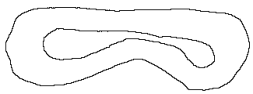
\includegraphics[interpolate=true,width=2.530000in,height=0.940000in]{contents/chapt7/figs/model/mu_wet_gravel_path-img0.png}}%
\end{pgfscope}%
\begin{pgfscope}%
\pgfpathrectangle{\pgfqpoint{0.150000in}{0.508846in}}{\pgfqpoint{2.525000in}{0.932308in}}%
\pgfusepath{clip}%
\pgfsetbuttcap%
\pgfsetroundjoin%
\pgfsetlinewidth{1.505625pt}%
\definecolor{currentstroke}{rgb}{1.000000,0.000000,0.000000}%
\pgfsetstrokecolor{currentstroke}%
\pgfsetdash{{1.500000pt}{2.475000pt}}{0.000000pt}%
\pgfpathmoveto{\pgfqpoint{1.698327in}{1.057765in}}%
\pgfpathlineto{\pgfqpoint{1.698327in}{1.368534in}}%
\pgfusepath{stroke}%
\end{pgfscope}%
\begin{pgfscope}%
\pgfpathrectangle{\pgfqpoint{0.150000in}{0.508846in}}{\pgfqpoint{2.525000in}{0.932308in}}%
\pgfusepath{clip}%
\pgfsetrectcap%
\pgfsetroundjoin%
\pgfsetlinewidth{1.505625pt}%
\definecolor{currentstroke}{rgb}{0.121569,0.466667,0.705882}%
\pgfsetstrokecolor{currentstroke}%
\pgfsetstrokeopacity{0.700000}%
\pgfsetdash{}{0pt}%
\pgfpathmoveto{\pgfqpoint{1.703846in}{1.208077in}}%
\pgfpathlineto{\pgfqpoint{1.638713in}{1.209064in}}%
\pgfpathlineto{\pgfqpoint{1.575923in}{1.212384in}}%
\pgfpathlineto{\pgfqpoint{1.484420in}{1.219804in}}%
\pgfpathlineto{\pgfqpoint{1.355522in}{1.230769in}}%
\pgfpathlineto{\pgfqpoint{1.292853in}{1.233644in}}%
\pgfpathlineto{\pgfqpoint{1.198758in}{1.235017in}}%
\pgfpathlineto{\pgfqpoint{0.947815in}{1.235600in}}%
\pgfpathlineto{\pgfqpoint{0.885129in}{1.233122in}}%
\pgfpathlineto{\pgfqpoint{0.830394in}{1.228960in}}%
\pgfpathlineto{\pgfqpoint{0.775864in}{1.222665in}}%
\pgfpathlineto{\pgfqpoint{0.721640in}{1.214122in}}%
\pgfpathlineto{\pgfqpoint{0.667827in}{1.203294in}}%
\pgfpathlineto{\pgfqpoint{0.629886in}{1.193426in}}%
\pgfpathlineto{\pgfqpoint{0.600258in}{1.183147in}}%
\pgfpathlineto{\pgfqpoint{0.578760in}{1.173602in}}%
\pgfpathlineto{\pgfqpoint{0.558153in}{1.162267in}}%
\pgfpathlineto{\pgfqpoint{0.538746in}{1.148983in}}%
\pgfpathlineto{\pgfqpoint{0.520875in}{1.133699in}}%
\pgfpathlineto{\pgfqpoint{0.504990in}{1.116362in}}%
\pgfpathlineto{\pgfqpoint{0.491442in}{1.097146in}}%
\pgfpathlineto{\pgfqpoint{0.480587in}{1.076292in}}%
\pgfpathlineto{\pgfqpoint{0.472720in}{1.054138in}}%
\pgfpathlineto{\pgfqpoint{0.469263in}{1.038843in}}%
\pgfpathlineto{\pgfqpoint{0.467298in}{1.023287in}}%
\pgfpathlineto{\pgfqpoint{0.466859in}{1.007613in}}%
\pgfpathlineto{\pgfqpoint{0.468930in}{0.984193in}}%
\pgfpathlineto{\pgfqpoint{0.473983in}{0.961228in}}%
\pgfpathlineto{\pgfqpoint{0.481655in}{0.939000in}}%
\pgfpathlineto{\pgfqpoint{0.491684in}{0.917728in}}%
\pgfpathlineto{\pgfqpoint{0.503743in}{0.897535in}}%
\pgfpathlineto{\pgfqpoint{0.517554in}{0.878496in}}%
\pgfpathlineto{\pgfqpoint{0.532870in}{0.860645in}}%
\pgfpathlineto{\pgfqpoint{0.555223in}{0.838651in}}%
\pgfpathlineto{\pgfqpoint{0.579450in}{0.818739in}}%
\pgfpathlineto{\pgfqpoint{0.605248in}{0.800907in}}%
\pgfpathlineto{\pgfqpoint{0.632371in}{0.785162in}}%
\pgfpathlineto{\pgfqpoint{0.660612in}{0.771522in}}%
\pgfpathlineto{\pgfqpoint{0.689839in}{0.760150in}}%
\pgfpathlineto{\pgfqpoint{0.719883in}{0.751158in}}%
\pgfpathlineto{\pgfqpoint{0.750565in}{0.744667in}}%
\pgfpathlineto{\pgfqpoint{0.781685in}{0.740790in}}%
\pgfpathlineto{\pgfqpoint{0.813022in}{0.739606in}}%
\pgfpathlineto{\pgfqpoint{0.844357in}{0.740918in}}%
\pgfpathlineto{\pgfqpoint{0.875507in}{0.744566in}}%
\pgfpathlineto{\pgfqpoint{0.906326in}{0.750387in}}%
\pgfpathlineto{\pgfqpoint{0.936700in}{0.758207in}}%
\pgfpathlineto{\pgfqpoint{0.966534in}{0.767884in}}%
\pgfpathlineto{\pgfqpoint{1.010367in}{0.784978in}}%
\pgfpathlineto{\pgfqpoint{1.060553in}{0.807219in}}%
\pgfpathlineto{\pgfqpoint{1.196211in}{0.868828in}}%
\pgfpathlineto{\pgfqpoint{1.254536in}{0.891930in}}%
\pgfpathlineto{\pgfqpoint{1.306372in}{0.909993in}}%
\pgfpathlineto{\pgfqpoint{1.358906in}{0.925908in}}%
\pgfpathlineto{\pgfqpoint{1.412080in}{0.939528in}}%
\pgfpathlineto{\pgfqpoint{1.450543in}{0.947131in}}%
\pgfpathlineto{\pgfqpoint{1.489390in}{0.952408in}}%
\pgfpathlineto{\pgfqpoint{1.520677in}{0.954617in}}%
\pgfpathlineto{\pgfqpoint{1.552032in}{0.954829in}}%
\pgfpathlineto{\pgfqpoint{1.590986in}{0.952468in}}%
\pgfpathlineto{\pgfqpoint{1.629454in}{0.947370in}}%
\pgfpathlineto{\pgfqpoint{1.667280in}{0.939762in}}%
\pgfpathlineto{\pgfqpoint{1.704334in}{0.929921in}}%
\pgfpathlineto{\pgfqpoint{1.740051in}{0.918009in}}%
\pgfpathlineto{\pgfqpoint{1.774099in}{0.903999in}}%
\pgfpathlineto{\pgfqpoint{1.799993in}{0.891263in}}%
\pgfpathlineto{\pgfqpoint{1.824566in}{0.877177in}}%
\pgfpathlineto{\pgfqpoint{1.853197in}{0.857893in}}%
\pgfpathlineto{\pgfqpoint{1.879354in}{0.837206in}}%
\pgfpathlineto{\pgfqpoint{1.903010in}{0.815388in}}%
\pgfpathlineto{\pgfqpoint{1.924237in}{0.792780in}}%
\pgfpathlineto{\pgfqpoint{1.947643in}{0.764219in}}%
\pgfpathlineto{\pgfqpoint{1.980259in}{0.724642in}}%
\pgfpathlineto{\pgfqpoint{2.003347in}{0.700726in}}%
\pgfpathlineto{\pgfqpoint{2.023844in}{0.682663in}}%
\pgfpathlineto{\pgfqpoint{2.046656in}{0.666033in}}%
\pgfpathlineto{\pgfqpoint{2.065365in}{0.654861in}}%
\pgfpathlineto{\pgfqpoint{2.085399in}{0.645029in}}%
\pgfpathlineto{\pgfqpoint{2.106696in}{0.636769in}}%
\pgfpathlineto{\pgfqpoint{2.129090in}{0.630296in}}%
\pgfpathlineto{\pgfqpoint{2.152050in}{0.625954in}}%
\pgfpathlineto{\pgfqpoint{2.175328in}{0.623915in}}%
\pgfpathlineto{\pgfqpoint{2.198690in}{0.624357in}}%
\pgfpathlineto{\pgfqpoint{2.221848in}{0.627450in}}%
\pgfpathlineto{\pgfqpoint{2.244481in}{0.633247in}}%
\pgfpathlineto{\pgfqpoint{2.266243in}{0.641748in}}%
\pgfpathlineto{\pgfqpoint{2.286797in}{0.652854in}}%
\pgfpathlineto{\pgfqpoint{2.305807in}{0.666397in}}%
\pgfpathlineto{\pgfqpoint{2.323100in}{0.681973in}}%
\pgfpathlineto{\pgfqpoint{2.338663in}{0.699188in}}%
\pgfpathlineto{\pgfqpoint{2.352458in}{0.717765in}}%
\pgfpathlineto{\pgfqpoint{2.364501in}{0.737443in}}%
\pgfpathlineto{\pgfqpoint{2.374882in}{0.757971in}}%
\pgfpathlineto{\pgfqpoint{2.386275in}{0.786334in}}%
\pgfpathlineto{\pgfqpoint{2.393026in}{0.808216in}}%
\pgfpathlineto{\pgfqpoint{2.399532in}{0.838020in}}%
\pgfpathlineto{\pgfqpoint{2.403176in}{0.868285in}}%
\pgfpathlineto{\pgfqpoint{2.403981in}{0.891122in}}%
\pgfpathlineto{\pgfqpoint{2.403085in}{0.913943in}}%
\pgfpathlineto{\pgfqpoint{2.400476in}{0.936659in}}%
\pgfpathlineto{\pgfqpoint{2.396039in}{0.959410in}}%
\pgfpathlineto{\pgfqpoint{2.389649in}{0.981938in}}%
\pgfpathlineto{\pgfqpoint{2.381381in}{1.003845in}}%
\pgfpathlineto{\pgfqpoint{2.371188in}{1.024925in}}%
\pgfpathlineto{\pgfqpoint{2.359041in}{1.044942in}}%
\pgfpathlineto{\pgfqpoint{2.344936in}{1.063630in}}%
\pgfpathlineto{\pgfqpoint{2.328951in}{1.080736in}}%
\pgfpathlineto{\pgfqpoint{2.311314in}{1.096137in}}%
\pgfpathlineto{\pgfqpoint{2.292349in}{1.109871in}}%
\pgfpathlineto{\pgfqpoint{2.272274in}{1.121926in}}%
\pgfpathlineto{\pgfqpoint{2.251293in}{1.132326in}}%
\pgfpathlineto{\pgfqpoint{2.222247in}{1.143771in}}%
\pgfpathlineto{\pgfqpoint{2.192310in}{1.152637in}}%
\pgfpathlineto{\pgfqpoint{2.154172in}{1.160935in}}%
\pgfpathlineto{\pgfqpoint{2.115603in}{1.166935in}}%
\pgfpathlineto{\pgfqpoint{2.061270in}{1.172799in}}%
\pgfpathlineto{\pgfqpoint{1.960064in}{1.180467in}}%
\pgfpathlineto{\pgfqpoint{1.843335in}{1.189915in}}%
\pgfpathlineto{\pgfqpoint{1.750158in}{1.199681in}}%
\pgfpathlineto{\pgfqpoint{1.750158in}{1.199681in}}%
\pgfusepath{stroke}%
\end{pgfscope}%
\begin{pgfscope}%
\pgfpathrectangle{\pgfqpoint{0.150000in}{0.508846in}}{\pgfqpoint{2.525000in}{0.932308in}}%
\pgfusepath{clip}%
\pgfsetrectcap%
\pgfsetroundjoin%
\pgfsetlinewidth{1.505625pt}%
\definecolor{currentstroke}{rgb}{1.000000,0.498039,0.054902}%
\pgfsetstrokecolor{currentstroke}%
\pgfsetstrokeopacity{0.700000}%
\pgfsetdash{}{0pt}%
\pgfpathmoveto{\pgfqpoint{1.703846in}{1.208077in}}%
\pgfpathlineto{\pgfqpoint{1.616491in}{1.209121in}}%
\pgfpathlineto{\pgfqpoint{1.537755in}{1.212398in}}%
\pgfpathlineto{\pgfqpoint{1.432901in}{1.219063in}}%
\pgfpathlineto{\pgfqpoint{1.301318in}{1.229603in}}%
\pgfpathlineto{\pgfqpoint{1.036932in}{1.251918in}}%
\pgfpathlineto{\pgfqpoint{0.966765in}{1.254941in}}%
\pgfpathlineto{\pgfqpoint{0.912141in}{1.255276in}}%
\pgfpathlineto{\pgfqpoint{0.857550in}{1.253383in}}%
\pgfpathlineto{\pgfqpoint{0.803105in}{1.248973in}}%
\pgfpathlineto{\pgfqpoint{0.756644in}{1.243177in}}%
\pgfpathlineto{\pgfqpoint{0.702781in}{1.234094in}}%
\pgfpathlineto{\pgfqpoint{0.656986in}{1.224347in}}%
\pgfpathlineto{\pgfqpoint{0.619285in}{1.214307in}}%
\pgfpathlineto{\pgfqpoint{0.582268in}{1.201989in}}%
\pgfpathlineto{\pgfqpoint{0.553362in}{1.190217in}}%
\pgfpathlineto{\pgfqpoint{0.525343in}{1.176470in}}%
\pgfpathlineto{\pgfqpoint{0.498582in}{1.160420in}}%
\pgfpathlineto{\pgfqpoint{0.479606in}{1.146715in}}%
\pgfpathlineto{\pgfqpoint{0.461774in}{1.131554in}}%
\pgfpathlineto{\pgfqpoint{0.445300in}{1.114928in}}%
\pgfpathlineto{\pgfqpoint{0.430399in}{1.096880in}}%
\pgfpathlineto{\pgfqpoint{0.417297in}{1.077487in}}%
\pgfpathlineto{\pgfqpoint{0.406167in}{1.056900in}}%
\pgfpathlineto{\pgfqpoint{0.397138in}{1.035308in}}%
\pgfpathlineto{\pgfqpoint{0.390351in}{1.012911in}}%
\pgfpathlineto{\pgfqpoint{0.385910in}{0.989934in}}%
\pgfpathlineto{\pgfqpoint{0.383866in}{0.966620in}}%
\pgfpathlineto{\pgfqpoint{0.384242in}{0.943220in}}%
\pgfpathlineto{\pgfqpoint{0.387017in}{0.919983in}}%
\pgfpathlineto{\pgfqpoint{0.392068in}{0.897130in}}%
\pgfpathlineto{\pgfqpoint{0.399175in}{0.874830in}}%
\pgfpathlineto{\pgfqpoint{0.408167in}{0.853220in}}%
\pgfpathlineto{\pgfqpoint{0.418895in}{0.832416in}}%
\pgfpathlineto{\pgfqpoint{0.431188in}{0.812497in}}%
\pgfpathlineto{\pgfqpoint{0.449697in}{0.787373in}}%
\pgfpathlineto{\pgfqpoint{0.470323in}{0.763952in}}%
\pgfpathlineto{\pgfqpoint{0.492740in}{0.742239in}}%
\pgfpathlineto{\pgfqpoint{0.516682in}{0.722218in}}%
\pgfpathlineto{\pgfqpoint{0.541942in}{0.703887in}}%
\pgfpathlineto{\pgfqpoint{0.568352in}{0.687253in}}%
\pgfpathlineto{\pgfqpoint{0.595790in}{0.672380in}}%
\pgfpathlineto{\pgfqpoint{0.624147in}{0.659341in}}%
\pgfpathlineto{\pgfqpoint{0.653302in}{0.648202in}}%
\pgfpathlineto{\pgfqpoint{0.683138in}{0.639042in}}%
\pgfpathlineto{\pgfqpoint{0.713444in}{0.631962in}}%
\pgfpathlineto{\pgfqpoint{0.743033in}{0.627164in}}%
\pgfpathlineto{\pgfqpoint{0.771490in}{0.624723in}}%
\pgfpathlineto{\pgfqpoint{0.798637in}{0.624785in}}%
\pgfpathlineto{\pgfqpoint{0.824228in}{0.627478in}}%
\pgfpathlineto{\pgfqpoint{0.847890in}{0.632826in}}%
\pgfpathlineto{\pgfqpoint{0.868694in}{0.640214in}}%
\pgfpathlineto{\pgfqpoint{0.886354in}{0.648972in}}%
\pgfpathlineto{\pgfqpoint{0.897722in}{0.656573in}}%
\pgfpathlineto{\pgfqpoint{0.911218in}{0.668828in}}%
\pgfpathlineto{\pgfqpoint{0.923022in}{0.682732in}}%
\pgfpathlineto{\pgfqpoint{0.938697in}{0.705163in}}%
\pgfpathlineto{\pgfqpoint{0.962109in}{0.738878in}}%
\pgfpathlineto{\pgfqpoint{0.979642in}{0.759885in}}%
\pgfpathlineto{\pgfqpoint{0.999239in}{0.779099in}}%
\pgfpathlineto{\pgfqpoint{1.017061in}{0.793571in}}%
\pgfpathlineto{\pgfqpoint{1.036142in}{0.806476in}}%
\pgfpathlineto{\pgfqpoint{1.056508in}{0.817844in}}%
\pgfpathlineto{\pgfqpoint{1.088610in}{0.832785in}}%
\pgfpathlineto{\pgfqpoint{1.141054in}{0.854467in}}%
\pgfpathlineto{\pgfqpoint{1.287328in}{0.911873in}}%
\pgfpathlineto{\pgfqpoint{1.343048in}{0.932362in}}%
\pgfpathlineto{\pgfqpoint{1.385145in}{0.945853in}}%
\pgfpathlineto{\pgfqpoint{1.420545in}{0.955285in}}%
\pgfpathlineto{\pgfqpoint{1.456367in}{0.962670in}}%
\pgfpathlineto{\pgfqpoint{1.492575in}{0.967702in}}%
\pgfpathlineto{\pgfqpoint{1.529033in}{0.970138in}}%
\pgfpathlineto{\pgfqpoint{1.565557in}{0.969862in}}%
\pgfpathlineto{\pgfqpoint{1.602032in}{0.967071in}}%
\pgfpathlineto{\pgfqpoint{1.638361in}{0.962155in}}%
\pgfpathlineto{\pgfqpoint{1.681664in}{0.953848in}}%
\pgfpathlineto{\pgfqpoint{1.731470in}{0.941670in}}%
\pgfpathlineto{\pgfqpoint{1.772613in}{0.929377in}}%
\pgfpathlineto{\pgfqpoint{1.812126in}{0.915334in}}%
\pgfpathlineto{\pgfqpoint{1.849714in}{0.899360in}}%
\pgfpathlineto{\pgfqpoint{1.878741in}{0.884489in}}%
\pgfpathlineto{\pgfqpoint{1.905277in}{0.868098in}}%
\pgfpathlineto{\pgfqpoint{1.924499in}{0.853846in}}%
\pgfpathlineto{\pgfqpoint{1.941752in}{0.838608in}}%
\pgfpathlineto{\pgfqpoint{1.957561in}{0.821755in}}%
\pgfpathlineto{\pgfqpoint{1.976062in}{0.798325in}}%
\pgfpathlineto{\pgfqpoint{2.008364in}{0.752018in}}%
\pgfpathlineto{\pgfqpoint{2.035477in}{0.714624in}}%
\pgfpathlineto{\pgfqpoint{2.057393in}{0.688597in}}%
\pgfpathlineto{\pgfqpoint{2.076930in}{0.668765in}}%
\pgfpathlineto{\pgfqpoint{2.098448in}{0.650251in}}%
\pgfpathlineto{\pgfqpoint{2.122059in}{0.633438in}}%
\pgfpathlineto{\pgfqpoint{2.141245in}{0.622130in}}%
\pgfpathlineto{\pgfqpoint{2.161648in}{0.612106in}}%
\pgfpathlineto{\pgfqpoint{2.183185in}{0.603493in}}%
\pgfpathlineto{\pgfqpoint{2.205474in}{0.596536in}}%
\pgfpathlineto{\pgfqpoint{2.228250in}{0.591394in}}%
\pgfpathlineto{\pgfqpoint{2.251380in}{0.588210in}}%
\pgfpathlineto{\pgfqpoint{2.274219in}{0.587129in}}%
\pgfpathlineto{\pgfqpoint{2.296328in}{0.588241in}}%
\pgfpathlineto{\pgfqpoint{2.317456in}{0.591699in}}%
\pgfpathlineto{\pgfqpoint{2.337270in}{0.597623in}}%
\pgfpathlineto{\pgfqpoint{2.355342in}{0.606080in}}%
\pgfpathlineto{\pgfqpoint{2.366176in}{0.613092in}}%
\pgfpathlineto{\pgfqpoint{2.375850in}{0.621136in}}%
\pgfpathlineto{\pgfqpoint{2.384217in}{0.630136in}}%
\pgfpathlineto{\pgfqpoint{2.391162in}{0.640022in}}%
\pgfpathlineto{\pgfqpoint{2.396594in}{0.650582in}}%
\pgfpathlineto{\pgfqpoint{2.400469in}{0.661590in}}%
\pgfpathlineto{\pgfqpoint{2.402792in}{0.672815in}}%
\pgfpathlineto{\pgfqpoint{2.403510in}{0.689596in}}%
\pgfpathlineto{\pgfqpoint{2.401257in}{0.705777in}}%
\pgfpathlineto{\pgfqpoint{2.396566in}{0.720945in}}%
\pgfpathlineto{\pgfqpoint{2.390015in}{0.734921in}}%
\pgfpathlineto{\pgfqpoint{2.381941in}{0.747700in}}%
\pgfpathlineto{\pgfqpoint{2.369368in}{0.762838in}}%
\pgfpathlineto{\pgfqpoint{2.355348in}{0.775874in}}%
\pgfpathlineto{\pgfqpoint{2.340310in}{0.786887in}}%
\pgfpathlineto{\pgfqpoint{2.324189in}{0.796041in}}%
\pgfpathlineto{\pgfqpoint{2.307126in}{0.803290in}}%
\pgfpathlineto{\pgfqpoint{2.289361in}{0.808592in}}%
\pgfpathlineto{\pgfqpoint{2.271111in}{0.811850in}}%
\pgfpathlineto{\pgfqpoint{2.261875in}{0.812681in}}%
\pgfpathlineto{\pgfqpoint{2.261875in}{0.812681in}}%
\pgfusepath{stroke}%
\end{pgfscope}%
\begin{pgfscope}%
\definecolor{textcolor}{rgb}{0.000000,0.000000,0.000000}%
\pgfsetstrokecolor{textcolor}%
\pgfsetfillcolor{textcolor}%
\pgftext[x=1.412500in,y=1.524487in,,base]{\color{textcolor}\rmfamily\fontsize{12.000000}{14.400000}\selectfont End-to-end}%
\end{pgfscope}%
\begin{pgfscope}%
\pgfpathrectangle{\pgfqpoint{2.825000in}{0.508846in}}{\pgfqpoint{2.525000in}{0.932308in}}%
\pgfusepath{clip}%
\pgfsys@transformshift{2.825000in}{0.508846in}%
\pgftext[left,bottom]{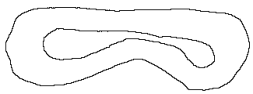
\includegraphics[interpolate=true,width=2.530000in,height=0.940000in]{contents/chapt7/figs/model/mu_wet_gravel_path-img1.png}}%
\end{pgfscope}%
\begin{pgfscope}%
\pgfpathrectangle{\pgfqpoint{2.825000in}{0.508846in}}{\pgfqpoint{2.525000in}{0.932308in}}%
\pgfusepath{clip}%
\pgfsetbuttcap%
\pgfsetroundjoin%
\pgfsetlinewidth{1.505625pt}%
\definecolor{currentstroke}{rgb}{1.000000,0.000000,0.000000}%
\pgfsetstrokecolor{currentstroke}%
\pgfsetdash{{1.500000pt}{2.475000pt}}{0.000000pt}%
\pgfpathmoveto{\pgfqpoint{4.373327in}{1.057765in}}%
\pgfpathlineto{\pgfqpoint{4.373327in}{1.368534in}}%
\pgfusepath{stroke}%
\end{pgfscope}%
\begin{pgfscope}%
\pgfpathrectangle{\pgfqpoint{2.825000in}{0.508846in}}{\pgfqpoint{2.525000in}{0.932308in}}%
\pgfusepath{clip}%
\pgfsetrectcap%
\pgfsetroundjoin%
\pgfsetlinewidth{1.505625pt}%
\definecolor{currentstroke}{rgb}{0.121569,0.466667,0.705882}%
\pgfsetstrokecolor{currentstroke}%
\pgfsetstrokeopacity{0.700000}%
\pgfsetdash{}{0pt}%
\pgfpathmoveto{\pgfqpoint{4.378846in}{1.208077in}}%
\pgfpathlineto{\pgfqpoint{4.319626in}{1.209089in}}%
\pgfpathlineto{\pgfqpoint{4.267947in}{1.212562in}}%
\pgfpathlineto{\pgfqpoint{4.197895in}{1.220134in}}%
\pgfpathlineto{\pgfqpoint{4.131732in}{1.226378in}}%
\pgfpathlineto{\pgfqpoint{4.071331in}{1.229610in}}%
\pgfpathlineto{\pgfqpoint{4.002570in}{1.230856in}}%
\pgfpathlineto{\pgfqpoint{3.909871in}{1.230093in}}%
\pgfpathlineto{\pgfqpoint{3.840192in}{1.227343in}}%
\pgfpathlineto{\pgfqpoint{3.778309in}{1.222690in}}%
\pgfpathlineto{\pgfqpoint{3.708875in}{1.215323in}}%
\pgfpathlineto{\pgfqpoint{3.624102in}{1.204100in}}%
\pgfpathlineto{\pgfqpoint{3.531736in}{1.192372in}}%
\pgfpathlineto{\pgfqpoint{3.470067in}{1.186886in}}%
\pgfpathlineto{\pgfqpoint{3.385108in}{1.179741in}}%
\pgfpathlineto{\pgfqpoint{3.346722in}{1.174119in}}%
\pgfpathlineto{\pgfqpoint{3.316384in}{1.167605in}}%
\pgfpathlineto{\pgfqpoint{3.286716in}{1.158731in}}%
\pgfpathlineto{\pgfqpoint{3.265135in}{1.150339in}}%
\pgfpathlineto{\pgfqpoint{3.244231in}{1.140269in}}%
\pgfpathlineto{\pgfqpoint{3.224253in}{1.128462in}}%
\pgfpathlineto{\pgfqpoint{3.205352in}{1.114911in}}%
\pgfpathlineto{\pgfqpoint{3.187790in}{1.099631in}}%
\pgfpathlineto{\pgfqpoint{3.171827in}{1.082692in}}%
\pgfpathlineto{\pgfqpoint{3.157640in}{1.064187in}}%
\pgfpathlineto{\pgfqpoint{3.145486in}{1.044318in}}%
\pgfpathlineto{\pgfqpoint{3.135542in}{1.023276in}}%
\pgfpathlineto{\pgfqpoint{3.127965in}{1.001233in}}%
\pgfpathlineto{\pgfqpoint{3.122876in}{0.978493in}}%
\pgfpathlineto{\pgfqpoint{3.120368in}{0.955328in}}%
\pgfpathlineto{\pgfqpoint{3.120476in}{0.932040in}}%
\pgfpathlineto{\pgfqpoint{3.123228in}{0.908919in}}%
\pgfpathlineto{\pgfqpoint{3.128584in}{0.886257in}}%
\pgfpathlineto{\pgfqpoint{3.136496in}{0.864332in}}%
\pgfpathlineto{\pgfqpoint{3.146834in}{0.843449in}}%
\pgfpathlineto{\pgfqpoint{3.159464in}{0.823853in}}%
\pgfpathlineto{\pgfqpoint{3.174082in}{0.805698in}}%
\pgfpathlineto{\pgfqpoint{3.190508in}{0.789166in}}%
\pgfpathlineto{\pgfqpoint{3.208490in}{0.774399in}}%
\pgfpathlineto{\pgfqpoint{3.227798in}{0.761523in}}%
\pgfpathlineto{\pgfqpoint{3.248290in}{0.750567in}}%
\pgfpathlineto{\pgfqpoint{3.269794in}{0.741556in}}%
\pgfpathlineto{\pgfqpoint{3.291993in}{0.734449in}}%
\pgfpathlineto{\pgfqpoint{3.314689in}{0.729080in}}%
\pgfpathlineto{\pgfqpoint{3.345447in}{0.724536in}}%
\pgfpathlineto{\pgfqpoint{3.376456in}{0.722789in}}%
\pgfpathlineto{\pgfqpoint{3.407485in}{0.723648in}}%
\pgfpathlineto{\pgfqpoint{3.438368in}{0.726961in}}%
\pgfpathlineto{\pgfqpoint{3.476566in}{0.733863in}}%
\pgfpathlineto{\pgfqpoint{3.521837in}{0.744421in}}%
\pgfpathlineto{\pgfqpoint{3.626963in}{0.772075in}}%
\pgfpathlineto{\pgfqpoint{3.776922in}{0.812788in}}%
\pgfpathlineto{\pgfqpoint{3.978779in}{0.869734in}}%
\pgfpathlineto{\pgfqpoint{4.024549in}{0.879124in}}%
\pgfpathlineto{\pgfqpoint{4.063046in}{0.884894in}}%
\pgfpathlineto{\pgfqpoint{4.101777in}{0.888456in}}%
\pgfpathlineto{\pgfqpoint{4.140625in}{0.889628in}}%
\pgfpathlineto{\pgfqpoint{4.179474in}{0.888497in}}%
\pgfpathlineto{\pgfqpoint{4.218169in}{0.885127in}}%
\pgfpathlineto{\pgfqpoint{4.256609in}{0.879649in}}%
\pgfpathlineto{\pgfqpoint{4.294716in}{0.872100in}}%
\pgfpathlineto{\pgfqpoint{4.332324in}{0.862331in}}%
\pgfpathlineto{\pgfqpoint{4.376702in}{0.848084in}}%
\pgfpathlineto{\pgfqpoint{4.472573in}{0.816196in}}%
\pgfpathlineto{\pgfqpoint{4.517562in}{0.803817in}}%
\pgfpathlineto{\pgfqpoint{4.600563in}{0.783579in}}%
\pgfpathlineto{\pgfqpoint{4.699260in}{0.761460in}}%
\pgfpathlineto{\pgfqpoint{4.745067in}{0.753269in}}%
\pgfpathlineto{\pgfqpoint{4.783538in}{0.748512in}}%
\pgfpathlineto{\pgfqpoint{4.814468in}{0.746589in}}%
\pgfpathlineto{\pgfqpoint{4.845538in}{0.746826in}}%
\pgfpathlineto{\pgfqpoint{4.876437in}{0.749540in}}%
\pgfpathlineto{\pgfqpoint{4.899374in}{0.753444in}}%
\pgfpathlineto{\pgfqpoint{4.921997in}{0.759074in}}%
\pgfpathlineto{\pgfqpoint{4.944131in}{0.766490in}}%
\pgfpathlineto{\pgfqpoint{4.965480in}{0.775749in}}%
\pgfpathlineto{\pgfqpoint{4.985863in}{0.786877in}}%
\pgfpathlineto{\pgfqpoint{5.005035in}{0.799853in}}%
\pgfpathlineto{\pgfqpoint{5.022769in}{0.814716in}}%
\pgfpathlineto{\pgfqpoint{5.038819in}{0.831354in}}%
\pgfpathlineto{\pgfqpoint{5.052999in}{0.849643in}}%
\pgfpathlineto{\pgfqpoint{5.065116in}{0.869426in}}%
\pgfpathlineto{\pgfqpoint{5.075016in}{0.890455in}}%
\pgfpathlineto{\pgfqpoint{5.082533in}{0.912419in}}%
\pgfpathlineto{\pgfqpoint{5.087566in}{0.935049in}}%
\pgfpathlineto{\pgfqpoint{5.090011in}{0.958058in}}%
\pgfpathlineto{\pgfqpoint{5.089831in}{0.981220in}}%
\pgfpathlineto{\pgfqpoint{5.087012in}{1.004195in}}%
\pgfpathlineto{\pgfqpoint{5.081597in}{1.026713in}}%
\pgfpathlineto{\pgfqpoint{5.073683in}{1.048457in}}%
\pgfpathlineto{\pgfqpoint{5.063442in}{1.069185in}}%
\pgfpathlineto{\pgfqpoint{5.051032in}{1.088631in}}%
\pgfpathlineto{\pgfqpoint{5.036601in}{1.106584in}}%
\pgfpathlineto{\pgfqpoint{5.020300in}{1.122916in}}%
\pgfpathlineto{\pgfqpoint{5.002369in}{1.137550in}}%
\pgfpathlineto{\pgfqpoint{4.983024in}{1.150423in}}%
\pgfpathlineto{\pgfqpoint{4.962584in}{1.161616in}}%
\pgfpathlineto{\pgfqpoint{4.941292in}{1.171103in}}%
\pgfpathlineto{\pgfqpoint{4.919347in}{1.178917in}}%
\pgfpathlineto{\pgfqpoint{4.889303in}{1.186820in}}%
\pgfpathlineto{\pgfqpoint{4.858721in}{1.192038in}}%
\pgfpathlineto{\pgfqpoint{4.827832in}{1.194839in}}%
\pgfpathlineto{\pgfqpoint{4.781312in}{1.196274in}}%
\pgfpathlineto{\pgfqpoint{4.656987in}{1.198038in}}%
\pgfpathlineto{\pgfqpoint{4.595025in}{1.201534in}}%
\pgfpathlineto{\pgfqpoint{4.509859in}{1.208770in}}%
\pgfpathlineto{\pgfqpoint{4.401552in}{1.218596in}}%
\pgfpathlineto{\pgfqpoint{4.401552in}{1.218596in}}%
\pgfusepath{stroke}%
\end{pgfscope}%
\begin{pgfscope}%
\pgfpathrectangle{\pgfqpoint{2.825000in}{0.508846in}}{\pgfqpoint{2.525000in}{0.932308in}}%
\pgfusepath{clip}%
\pgfsetrectcap%
\pgfsetroundjoin%
\pgfsetlinewidth{1.505625pt}%
\definecolor{currentstroke}{rgb}{1.000000,0.498039,0.054902}%
\pgfsetstrokecolor{currentstroke}%
\pgfsetstrokeopacity{0.700000}%
\pgfsetdash{}{0pt}%
\pgfpathmoveto{\pgfqpoint{4.378846in}{1.208077in}}%
\pgfpathlineto{\pgfqpoint{4.301040in}{1.209031in}}%
\pgfpathlineto{\pgfqpoint{4.240916in}{1.211911in}}%
\pgfpathlineto{\pgfqpoint{4.154328in}{1.218598in}}%
\pgfpathlineto{\pgfqpoint{3.971973in}{1.233805in}}%
\pgfpathlineto{\pgfqpoint{3.894790in}{1.237393in}}%
\pgfpathlineto{\pgfqpoint{3.825092in}{1.238128in}}%
\pgfpathlineto{\pgfqpoint{3.763134in}{1.236530in}}%
\pgfpathlineto{\pgfqpoint{3.701140in}{1.232628in}}%
\pgfpathlineto{\pgfqpoint{3.639296in}{1.226329in}}%
\pgfpathlineto{\pgfqpoint{3.577788in}{1.217796in}}%
\pgfpathlineto{\pgfqpoint{3.509147in}{1.205917in}}%
\pgfpathlineto{\pgfqpoint{3.433288in}{1.190397in}}%
\pgfpathlineto{\pgfqpoint{3.365524in}{1.174357in}}%
\pgfpathlineto{\pgfqpoint{3.313112in}{1.159686in}}%
\pgfpathlineto{\pgfqpoint{3.276227in}{1.147283in}}%
\pgfpathlineto{\pgfqpoint{3.240200in}{1.132635in}}%
\pgfpathlineto{\pgfqpoint{3.212343in}{1.118919in}}%
\pgfpathlineto{\pgfqpoint{3.185598in}{1.103093in}}%
\pgfpathlineto{\pgfqpoint{3.160393in}{1.085006in}}%
\pgfpathlineto{\pgfqpoint{3.142710in}{1.069820in}}%
\pgfpathlineto{\pgfqpoint{3.126314in}{1.053268in}}%
\pgfpathlineto{\pgfqpoint{3.111379in}{1.035377in}}%
\pgfpathlineto{\pgfqpoint{3.098110in}{1.016236in}}%
\pgfpathlineto{\pgfqpoint{3.086711in}{0.996003in}}%
\pgfpathlineto{\pgfqpoint{3.077267in}{0.974803in}}%
\pgfpathlineto{\pgfqpoint{3.069851in}{0.952719in}}%
\pgfpathlineto{\pgfqpoint{3.064596in}{0.929986in}}%
\pgfpathlineto{\pgfqpoint{3.061591in}{0.906900in}}%
\pgfpathlineto{\pgfqpoint{3.060843in}{0.883583in}}%
\pgfpathlineto{\pgfqpoint{3.062359in}{0.860323in}}%
\pgfpathlineto{\pgfqpoint{3.066117in}{0.837325in}}%
\pgfpathlineto{\pgfqpoint{3.072011in}{0.814812in}}%
\pgfpathlineto{\pgfqpoint{3.079967in}{0.792947in}}%
\pgfpathlineto{\pgfqpoint{3.089936in}{0.771944in}}%
\pgfpathlineto{\pgfqpoint{3.101795in}{0.752006in}}%
\pgfpathlineto{\pgfqpoint{3.115450in}{0.733246in}}%
\pgfpathlineto{\pgfqpoint{3.130771in}{0.715823in}}%
\pgfpathlineto{\pgfqpoint{3.147602in}{0.699825in}}%
\pgfpathlineto{\pgfqpoint{3.165707in}{0.685291in}}%
\pgfpathlineto{\pgfqpoint{3.184959in}{0.672277in}}%
\pgfpathlineto{\pgfqpoint{3.205228in}{0.660797in}}%
\pgfpathlineto{\pgfqpoint{3.226339in}{0.650901in}}%
\pgfpathlineto{\pgfqpoint{3.248137in}{0.642608in}}%
\pgfpathlineto{\pgfqpoint{3.277999in}{0.634008in}}%
\pgfpathlineto{\pgfqpoint{3.308484in}{0.628047in}}%
\pgfpathlineto{\pgfqpoint{3.339348in}{0.624656in}}%
\pgfpathlineto{\pgfqpoint{3.370416in}{0.623741in}}%
\pgfpathlineto{\pgfqpoint{3.401448in}{0.625189in}}%
\pgfpathlineto{\pgfqpoint{3.432249in}{0.628917in}}%
\pgfpathlineto{\pgfqpoint{3.462763in}{0.634655in}}%
\pgfpathlineto{\pgfqpoint{3.500486in}{0.644070in}}%
\pgfpathlineto{\pgfqpoint{3.545051in}{0.657912in}}%
\pgfpathlineto{\pgfqpoint{3.596207in}{0.676451in}}%
\pgfpathlineto{\pgfqpoint{3.973386in}{0.821320in}}%
\pgfpathlineto{\pgfqpoint{4.066961in}{0.858732in}}%
\pgfpathlineto{\pgfqpoint{4.110853in}{0.874006in}}%
\pgfpathlineto{\pgfqpoint{4.148093in}{0.884903in}}%
\pgfpathlineto{\pgfqpoint{4.185903in}{0.893703in}}%
\pgfpathlineto{\pgfqpoint{4.224263in}{0.900088in}}%
\pgfpathlineto{\pgfqpoint{4.255137in}{0.903248in}}%
\pgfpathlineto{\pgfqpoint{4.286114in}{0.904508in}}%
\pgfpathlineto{\pgfqpoint{4.317064in}{0.903780in}}%
\pgfpathlineto{\pgfqpoint{4.347879in}{0.901118in}}%
\pgfpathlineto{\pgfqpoint{4.378543in}{0.896522in}}%
\pgfpathlineto{\pgfqpoint{4.408892in}{0.889965in}}%
\pgfpathlineto{\pgfqpoint{4.438809in}{0.881502in}}%
\pgfpathlineto{\pgfqpoint{4.468155in}{0.871219in}}%
\pgfpathlineto{\pgfqpoint{4.503997in}{0.856251in}}%
\pgfpathlineto{\pgfqpoint{4.546029in}{0.836179in}}%
\pgfpathlineto{\pgfqpoint{4.614826in}{0.800134in}}%
\pgfpathlineto{\pgfqpoint{4.676921in}{0.768398in}}%
\pgfpathlineto{\pgfqpoint{4.719192in}{0.749351in}}%
\pgfpathlineto{\pgfqpoint{4.755267in}{0.735512in}}%
\pgfpathlineto{\pgfqpoint{4.792147in}{0.724088in}}%
\pgfpathlineto{\pgfqpoint{4.822159in}{0.717018in}}%
\pgfpathlineto{\pgfqpoint{4.852660in}{0.712076in}}%
\pgfpathlineto{\pgfqpoint{4.883431in}{0.709495in}}%
\pgfpathlineto{\pgfqpoint{4.914276in}{0.709503in}}%
\pgfpathlineto{\pgfqpoint{4.944903in}{0.712295in}}%
\pgfpathlineto{\pgfqpoint{4.967627in}{0.716315in}}%
\pgfpathlineto{\pgfqpoint{4.989975in}{0.722032in}}%
\pgfpathlineto{\pgfqpoint{5.011880in}{0.729483in}}%
\pgfpathlineto{\pgfqpoint{5.033102in}{0.738633in}}%
\pgfpathlineto{\pgfqpoint{5.053513in}{0.749496in}}%
\pgfpathlineto{\pgfqpoint{5.073026in}{0.761978in}}%
\pgfpathlineto{\pgfqpoint{5.091474in}{0.776026in}}%
\pgfpathlineto{\pgfqpoint{5.108712in}{0.791576in}}%
\pgfpathlineto{\pgfqpoint{5.124600in}{0.808496in}}%
\pgfpathlineto{\pgfqpoint{5.139010in}{0.826705in}}%
\pgfpathlineto{\pgfqpoint{5.151804in}{0.846088in}}%
\pgfpathlineto{\pgfqpoint{5.162901in}{0.866477in}}%
\pgfpathlineto{\pgfqpoint{5.172281in}{0.887759in}}%
\pgfpathlineto{\pgfqpoint{5.179863in}{0.909802in}}%
\pgfpathlineto{\pgfqpoint{5.185545in}{0.932408in}}%
\pgfpathlineto{\pgfqpoint{5.189285in}{0.955365in}}%
\pgfpathlineto{\pgfqpoint{5.191056in}{0.978568in}}%
\pgfpathlineto{\pgfqpoint{5.190800in}{1.001861in}}%
\pgfpathlineto{\pgfqpoint{5.188591in}{1.025064in}}%
\pgfpathlineto{\pgfqpoint{5.184512in}{1.047978in}}%
\pgfpathlineto{\pgfqpoint{5.178551in}{1.070442in}}%
\pgfpathlineto{\pgfqpoint{5.170754in}{1.092320in}}%
\pgfpathlineto{\pgfqpoint{5.161140in}{1.113509in}}%
\pgfpathlineto{\pgfqpoint{5.149791in}{1.133812in}}%
\pgfpathlineto{\pgfqpoint{5.136826in}{1.153130in}}%
\pgfpathlineto{\pgfqpoint{5.122386in}{1.171373in}}%
\pgfpathlineto{\pgfqpoint{5.106573in}{1.188438in}}%
\pgfpathlineto{\pgfqpoint{5.089487in}{1.204240in}}%
\pgfpathlineto{\pgfqpoint{5.071214in}{1.218745in}}%
\pgfpathlineto{\pgfqpoint{5.051932in}{1.231821in}}%
\pgfpathlineto{\pgfqpoint{5.031763in}{1.243391in}}%
\pgfpathlineto{\pgfqpoint{5.003686in}{1.256498in}}%
\pgfpathlineto{\pgfqpoint{4.974611in}{1.267082in}}%
\pgfpathlineto{\pgfqpoint{4.944650in}{1.275198in}}%
\pgfpathlineto{\pgfqpoint{4.914076in}{1.280935in}}%
\pgfpathlineto{\pgfqpoint{4.883211in}{1.284433in}}%
\pgfpathlineto{\pgfqpoint{4.844472in}{1.286056in}}%
\pgfpathlineto{\pgfqpoint{4.797851in}{1.285226in}}%
\pgfpathlineto{\pgfqpoint{4.735691in}{1.281545in}}%
\pgfpathlineto{\pgfqpoint{4.619413in}{1.274458in}}%
\pgfpathlineto{\pgfqpoint{4.557391in}{1.272958in}}%
\pgfpathlineto{\pgfqpoint{4.433174in}{1.272675in}}%
\pgfpathlineto{\pgfqpoint{4.433174in}{1.272675in}}%
\pgfusepath{stroke}%
\end{pgfscope}%
\begin{pgfscope}%
\definecolor{textcolor}{rgb}{0.000000,0.000000,0.000000}%
\pgfsetstrokecolor{textcolor}%
\pgfsetfillcolor{textcolor}%
\pgftext[x=4.087500in,y=1.524487in,,base]{\color{textcolor}\rmfamily\fontsize{12.000000}{14.400000}\selectfont Steering and velocity control}%
\end{pgfscope}%
\begin{pgfscope}%
\pgfsetbuttcap%
\pgfsetmiterjoin%
\definecolor{currentfill}{rgb}{1.000000,1.000000,1.000000}%
\pgfsetfillcolor{currentfill}%
\pgfsetfillopacity{0.800000}%
\pgfsetlinewidth{1.003750pt}%
\definecolor{currentstroke}{rgb}{0.800000,0.800000,0.800000}%
\pgfsetstrokecolor{currentstroke}%
\pgfsetstrokeopacity{0.800000}%
\pgfsetdash{}{0pt}%
\pgfpathmoveto{\pgfqpoint{1.002903in}{0.069444in}}%
\pgfpathlineto{\pgfqpoint{4.497097in}{0.069444in}}%
\pgfpathquadraticcurveto{\pgfqpoint{4.524875in}{0.069444in}}{\pgfqpoint{4.524875in}{0.097222in}}%
\pgfpathlineto{\pgfqpoint{4.524875in}{0.442708in}}%
\pgfpathquadraticcurveto{\pgfqpoint{4.524875in}{0.470486in}}{\pgfqpoint{4.497097in}{0.470486in}}%
\pgfpathlineto{\pgfqpoint{1.002903in}{0.470486in}}%
\pgfpathquadraticcurveto{\pgfqpoint{0.975125in}{0.470486in}}{\pgfqpoint{0.975125in}{0.442708in}}%
\pgfpathlineto{\pgfqpoint{0.975125in}{0.097222in}}%
\pgfpathquadraticcurveto{\pgfqpoint{0.975125in}{0.069444in}}{\pgfqpoint{1.002903in}{0.069444in}}%
\pgfpathlineto{\pgfqpoint{1.002903in}{0.069444in}}%
\pgfpathclose%
\pgfusepath{stroke,fill}%
\end{pgfscope}%
\begin{pgfscope}%
\pgfsetrectcap%
\pgfsetroundjoin%
\pgfsetlinewidth{1.505625pt}%
\definecolor{currentstroke}{rgb}{0.121569,0.466667,0.705882}%
\pgfsetstrokecolor{currentstroke}%
\pgfsetstrokeopacity{0.700000}%
\pgfsetdash{}{0pt}%
\pgfpathmoveto{\pgfqpoint{1.030680in}{0.265815in}}%
\pgfpathlineto{\pgfqpoint{1.169569in}{0.265815in}}%
\pgfpathlineto{\pgfqpoint{1.308458in}{0.265815in}}%
\pgfusepath{stroke}%
\end{pgfscope}%
\begin{pgfscope}%
\definecolor{textcolor}{rgb}{0.000000,0.000000,0.000000}%
\pgfsetstrokecolor{textcolor}%
\pgfsetfillcolor{textcolor}%
\pgftext[x=1.419569in,y=0.217204in,left,base]{\color{textcolor}\rmfamily\fontsize{10.000000}{12.000000}\selectfont No model error}%
\end{pgfscope}%
\begin{pgfscope}%
\pgfsetrectcap%
\pgfsetroundjoin%
\pgfsetlinewidth{1.505625pt}%
\definecolor{currentstroke}{rgb}{1.000000,0.498039,0.054902}%
\pgfsetstrokecolor{currentstroke}%
\pgfsetstrokeopacity{0.700000}%
\pgfsetdash{}{0pt}%
\pgfpathmoveto{\pgfqpoint{2.786621in}{0.265815in}}%
\pgfpathlineto{\pgfqpoint{2.925510in}{0.265815in}}%
\pgfpathlineto{\pgfqpoint{3.064399in}{0.265815in}}%
\pgfusepath{stroke}%
\end{pgfscope}%
\begin{pgfscope}%
\definecolor{textcolor}{rgb}{0.000000,0.000000,0.000000}%
\pgfsetstrokecolor{textcolor}%
\pgfsetfillcolor{textcolor}%
\pgftext[x=3.175510in, y=0.309407in, left, base]{\color{textcolor}\rmfamily\fontsize{10.000000}{12.000000}\selectfont Decreased road }%
\end{pgfscope}%
\begin{pgfscope}%
\definecolor{textcolor}{rgb}{0.000000,0.000000,0.000000}%
\pgfsetstrokecolor{textcolor}%
\pgfsetfillcolor{textcolor}%
\pgftext[x=3.175510in, y=0.153890in, left, base]{\color{textcolor}\rmfamily\fontsize{10.000000}{12.000000}\selectfont friction coefficient}%
\end{pgfscope}%
\end{pgfpicture}%
\makeatother%
\endgroup%

%     \caption[]{}
%     \label{fig:mu_wet_gravel_path}
% \end{figure}

\begin{figure}[htb!]
    \centering
    %% Creator: Matplotlib, PGF backend
%%
%% To include the figure in your LaTeX document, write
%%   \input{<filename>.pgf}
%%
%% Make sure the required packages are loaded in your preamble
%%   \usepackage{pgf}
%%
%% Also ensure that all the required font packages are loaded; for instance,
%% the lmodern package is sometimes necessary when using math font.
%%   \usepackage{lmodern}
%%
%% Figures using additional raster images can only be included by \input if
%% they are in the same directory as the main LaTeX file. For loading figures
%% from other directories you can use the `import` package
%%   \usepackage{import}
%%
%% and then include the figures with
%%   \import{<path to file>}{<filename>.pgf}
%%
%% Matplotlib used the following preamble
%%   \usepackage{fontspec}
%%   \setmainfont{DejaVuSerif.ttf}[Path=\detokenize{/home/andrew/anaconda3/envs/auto_car_env/lib/python3.9/site-packages/matplotlib/mpl-data/fonts/ttf/}]
%%   \setsansfont{DejaVuSans.ttf}[Path=\detokenize{/home/andrew/anaconda3/envs/auto_car_env/lib/python3.9/site-packages/matplotlib/mpl-data/fonts/ttf/}]
%%   \setmonofont{DejaVuSansMono.ttf}[Path=\detokenize{/home/andrew/anaconda3/envs/auto_car_env/lib/python3.9/site-packages/matplotlib/mpl-data/fonts/ttf/}]
%%
\begingroup%
\makeatletter%
\begin{pgfpicture}%
\pgfpathrectangle{\pgfpointorigin}{\pgfqpoint{5.500000in}{2.000000in}}%
\pgfusepath{use as bounding box, clip}%
\begin{pgfscope}%
\pgfsetbuttcap%
\pgfsetmiterjoin%
\definecolor{currentfill}{rgb}{1.000000,1.000000,1.000000}%
\pgfsetfillcolor{currentfill}%
\pgfsetlinewidth{0.000000pt}%
\definecolor{currentstroke}{rgb}{1.000000,1.000000,1.000000}%
\pgfsetstrokecolor{currentstroke}%
\pgfsetdash{}{0pt}%
\pgfpathmoveto{\pgfqpoint{0.000000in}{0.000000in}}%
\pgfpathlineto{\pgfqpoint{5.500000in}{0.000000in}}%
\pgfpathlineto{\pgfqpoint{5.500000in}{2.000000in}}%
\pgfpathlineto{\pgfqpoint{0.000000in}{2.000000in}}%
\pgfpathlineto{\pgfqpoint{0.000000in}{0.000000in}}%
\pgfpathclose%
\pgfusepath{fill}%
\end{pgfscope}%
\begin{pgfscope}%
\pgfpathrectangle{\pgfqpoint{0.150000in}{0.508846in}}{\pgfqpoint{2.525000in}{0.932308in}}%
\pgfusepath{clip}%
\pgfsys@transformshift{0.150000in}{0.508846in}%
\pgftext[left,bottom]{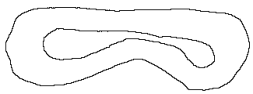
\includegraphics[interpolate=true,width=2.530000in,height=0.940000in]{contents/chapt7/figs/model/mu_paths-img0.png}}%
\end{pgfscope}%
\begin{pgfscope}%
\pgfpathrectangle{\pgfqpoint{0.150000in}{0.508846in}}{\pgfqpoint{2.525000in}{0.932308in}}%
\pgfusepath{clip}%
\pgfsetbuttcap%
\pgfsetroundjoin%
\pgfsetlinewidth{1.505625pt}%
\definecolor{currentstroke}{rgb}{1.000000,0.000000,0.000000}%
\pgfsetstrokecolor{currentstroke}%
\pgfsetdash{{1.500000pt}{2.475000pt}}{0.000000pt}%
\pgfpathmoveto{\pgfqpoint{1.698327in}{1.057765in}}%
\pgfpathlineto{\pgfqpoint{1.698327in}{1.368534in}}%
\pgfusepath{stroke}%
\end{pgfscope}%
\begin{pgfscope}%
\pgfpathrectangle{\pgfqpoint{0.150000in}{0.508846in}}{\pgfqpoint{2.525000in}{0.932308in}}%
\pgfusepath{clip}%
\pgfsetrectcap%
\pgfsetroundjoin%
\pgfsetlinewidth{1.505625pt}%
\definecolor{currentstroke}{rgb}{0.121569,0.466667,0.705882}%
\pgfsetstrokecolor{currentstroke}%
\pgfsetstrokeopacity{0.700000}%
\pgfsetdash{}{0pt}%
\pgfpathmoveto{\pgfqpoint{1.703846in}{1.208077in}}%
\pgfpathlineto{\pgfqpoint{1.638606in}{1.209063in}}%
\pgfpathlineto{\pgfqpoint{1.575555in}{1.212385in}}%
\pgfpathlineto{\pgfqpoint{1.483691in}{1.219816in}}%
\pgfpathlineto{\pgfqpoint{1.355115in}{1.230698in}}%
\pgfpathlineto{\pgfqpoint{1.292980in}{1.233456in}}%
\pgfpathlineto{\pgfqpoint{1.199689in}{1.234661in}}%
\pgfpathlineto{\pgfqpoint{0.950899in}{1.234854in}}%
\pgfpathlineto{\pgfqpoint{0.888754in}{1.232297in}}%
\pgfpathlineto{\pgfqpoint{0.834495in}{1.228088in}}%
\pgfpathlineto{\pgfqpoint{0.780442in}{1.221773in}}%
\pgfpathlineto{\pgfqpoint{0.726694in}{1.213239in}}%
\pgfpathlineto{\pgfqpoint{0.673352in}{1.202454in}}%
\pgfpathlineto{\pgfqpoint{0.635745in}{1.192636in}}%
\pgfpathlineto{\pgfqpoint{0.606383in}{1.182415in}}%
\pgfpathlineto{\pgfqpoint{0.585080in}{1.172927in}}%
\pgfpathlineto{\pgfqpoint{0.564662in}{1.161666in}}%
\pgfpathlineto{\pgfqpoint{0.545435in}{1.148477in}}%
\pgfpathlineto{\pgfqpoint{0.527728in}{1.133311in}}%
\pgfpathlineto{\pgfqpoint{0.511988in}{1.116116in}}%
\pgfpathlineto{\pgfqpoint{0.498556in}{1.097064in}}%
\pgfpathlineto{\pgfqpoint{0.487784in}{1.076394in}}%
\pgfpathlineto{\pgfqpoint{0.479960in}{1.054439in}}%
\pgfpathlineto{\pgfqpoint{0.475335in}{1.031595in}}%
\pgfpathlineto{\pgfqpoint{0.474105in}{1.016098in}}%
\pgfpathlineto{\pgfqpoint{0.475028in}{0.992808in}}%
\pgfpathlineto{\pgfqpoint{0.479004in}{0.969838in}}%
\pgfpathlineto{\pgfqpoint{0.485716in}{0.947512in}}%
\pgfpathlineto{\pgfqpoint{0.494938in}{0.926099in}}%
\pgfpathlineto{\pgfqpoint{0.506368in}{0.905777in}}%
\pgfpathlineto{\pgfqpoint{0.519738in}{0.886674in}}%
\pgfpathlineto{\pgfqpoint{0.534797in}{0.868870in}}%
\pgfpathlineto{\pgfqpoint{0.551284in}{0.852379in}}%
\pgfpathlineto{\pgfqpoint{0.569028in}{0.837247in}}%
\pgfpathlineto{\pgfqpoint{0.587861in}{0.823494in}}%
\pgfpathlineto{\pgfqpoint{0.614430in}{0.807350in}}%
\pgfpathlineto{\pgfqpoint{0.642389in}{0.793752in}}%
\pgfpathlineto{\pgfqpoint{0.671467in}{0.782749in}}%
\pgfpathlineto{\pgfqpoint{0.701376in}{0.774257in}}%
\pgfpathlineto{\pgfqpoint{0.731881in}{0.768245in}}%
\pgfpathlineto{\pgfqpoint{0.762767in}{0.764662in}}%
\pgfpathlineto{\pgfqpoint{0.793836in}{0.763448in}}%
\pgfpathlineto{\pgfqpoint{0.824911in}{0.764528in}}%
\pgfpathlineto{\pgfqpoint{0.855841in}{0.767724in}}%
\pgfpathlineto{\pgfqpoint{0.886497in}{0.772935in}}%
\pgfpathlineto{\pgfqpoint{0.916768in}{0.780048in}}%
\pgfpathlineto{\pgfqpoint{0.946559in}{0.788961in}}%
\pgfpathlineto{\pgfqpoint{0.982995in}{0.802493in}}%
\pgfpathlineto{\pgfqpoint{1.025757in}{0.821130in}}%
\pgfpathlineto{\pgfqpoint{1.167282in}{0.885496in}}%
\pgfpathlineto{\pgfqpoint{1.210988in}{0.901794in}}%
\pgfpathlineto{\pgfqpoint{1.255497in}{0.915743in}}%
\pgfpathlineto{\pgfqpoint{1.300663in}{0.927400in}}%
\pgfpathlineto{\pgfqpoint{1.346325in}{0.936928in}}%
\pgfpathlineto{\pgfqpoint{1.392349in}{0.944528in}}%
\pgfpathlineto{\pgfqpoint{1.438659in}{0.950103in}}%
\pgfpathlineto{\pgfqpoint{1.477441in}{0.952743in}}%
\pgfpathlineto{\pgfqpoint{1.516307in}{0.953253in}}%
\pgfpathlineto{\pgfqpoint{1.555130in}{0.951381in}}%
\pgfpathlineto{\pgfqpoint{1.593758in}{0.947050in}}%
\pgfpathlineto{\pgfqpoint{1.632056in}{0.940409in}}%
\pgfpathlineto{\pgfqpoint{1.669911in}{0.931586in}}%
\pgfpathlineto{\pgfqpoint{1.707231in}{0.920713in}}%
\pgfpathlineto{\pgfqpoint{1.743478in}{0.907958in}}%
\pgfpathlineto{\pgfqpoint{1.778178in}{0.893252in}}%
\pgfpathlineto{\pgfqpoint{1.811104in}{0.876490in}}%
\pgfpathlineto{\pgfqpoint{1.836010in}{0.861581in}}%
\pgfpathlineto{\pgfqpoint{1.865122in}{0.841271in}}%
\pgfpathlineto{\pgfqpoint{1.891975in}{0.819682in}}%
\pgfpathlineto{\pgfqpoint{1.916646in}{0.797150in}}%
\pgfpathlineto{\pgfqpoint{1.943603in}{0.769358in}}%
\pgfpathlineto{\pgfqpoint{2.015555in}{0.691046in}}%
\pgfpathlineto{\pgfqpoint{2.036516in}{0.672475in}}%
\pgfpathlineto{\pgfqpoint{2.059293in}{0.654996in}}%
\pgfpathlineto{\pgfqpoint{2.077790in}{0.642986in}}%
\pgfpathlineto{\pgfqpoint{2.097549in}{0.632226in}}%
\pgfpathlineto{\pgfqpoint{2.118535in}{0.622951in}}%
\pgfpathlineto{\pgfqpoint{2.140626in}{0.615416in}}%
\pgfpathlineto{\pgfqpoint{2.163378in}{0.609996in}}%
\pgfpathlineto{\pgfqpoint{2.186564in}{0.606943in}}%
\pgfpathlineto{\pgfqpoint{2.209946in}{0.606517in}}%
\pgfpathlineto{\pgfqpoint{2.233208in}{0.608893in}}%
\pgfpathlineto{\pgfqpoint{2.255984in}{0.614185in}}%
\pgfpathlineto{\pgfqpoint{2.277879in}{0.622389in}}%
\pgfpathlineto{\pgfqpoint{2.298485in}{0.633438in}}%
\pgfpathlineto{\pgfqpoint{2.317417in}{0.647159in}}%
\pgfpathlineto{\pgfqpoint{2.334293in}{0.663291in}}%
\pgfpathlineto{\pgfqpoint{2.348966in}{0.681383in}}%
\pgfpathlineto{\pgfqpoint{2.361463in}{0.700982in}}%
\pgfpathlineto{\pgfqpoint{2.371914in}{0.721686in}}%
\pgfpathlineto{\pgfqpoint{2.380409in}{0.743210in}}%
\pgfpathlineto{\pgfqpoint{2.387142in}{0.765294in}}%
\pgfpathlineto{\pgfqpoint{2.393670in}{0.795309in}}%
\pgfpathlineto{\pgfqpoint{2.397625in}{0.825776in}}%
\pgfpathlineto{\pgfqpoint{2.399218in}{0.856469in}}%
\pgfpathlineto{\pgfqpoint{2.398555in}{0.887208in}}%
\pgfpathlineto{\pgfqpoint{2.395684in}{0.917831in}}%
\pgfpathlineto{\pgfqpoint{2.390617in}{0.948285in}}%
\pgfpathlineto{\pgfqpoint{2.383080in}{0.978548in}}%
\pgfpathlineto{\pgfqpoint{2.375497in}{1.000677in}}%
\pgfpathlineto{\pgfqpoint{2.366099in}{1.022097in}}%
\pgfpathlineto{\pgfqpoint{2.354779in}{1.042565in}}%
\pgfpathlineto{\pgfqpoint{2.341441in}{1.061776in}}%
\pgfpathlineto{\pgfqpoint{2.326095in}{1.079425in}}%
\pgfpathlineto{\pgfqpoint{2.308937in}{1.095318in}}%
\pgfpathlineto{\pgfqpoint{2.290299in}{1.109450in}}%
\pgfpathlineto{\pgfqpoint{2.270444in}{1.121817in}}%
\pgfpathlineto{\pgfqpoint{2.249606in}{1.132444in}}%
\pgfpathlineto{\pgfqpoint{2.227998in}{1.141407in}}%
\pgfpathlineto{\pgfqpoint{2.198308in}{1.150954in}}%
\pgfpathlineto{\pgfqpoint{2.167944in}{1.158089in}}%
\pgfpathlineto{\pgfqpoint{2.129521in}{1.164723in}}%
\pgfpathlineto{\pgfqpoint{2.075334in}{1.171354in}}%
\pgfpathlineto{\pgfqpoint{1.834979in}{1.197448in}}%
\pgfpathlineto{\pgfqpoint{1.757378in}{1.205204in}}%
\pgfpathlineto{\pgfqpoint{1.741823in}{1.206375in}}%
\pgfpathlineto{\pgfqpoint{1.741823in}{1.206375in}}%
\pgfusepath{stroke}%
\end{pgfscope}%
\begin{pgfscope}%
\pgfpathrectangle{\pgfqpoint{0.150000in}{0.508846in}}{\pgfqpoint{2.525000in}{0.932308in}}%
\pgfusepath{clip}%
\pgfsetbuttcap%
\pgfsetroundjoin%
\pgfsetlinewidth{1.505625pt}%
\definecolor{currentstroke}{rgb}{1.000000,0.498039,0.054902}%
\pgfsetstrokecolor{currentstroke}%
\pgfsetstrokeopacity{0.700000}%
\pgfsetdash{{5.550000pt}{2.400000pt}}{0.000000pt}%
\pgfpathmoveto{\pgfqpoint{1.703846in}{1.208077in}}%
\pgfpathlineto{\pgfqpoint{1.616508in}{1.209121in}}%
\pgfpathlineto{\pgfqpoint{1.537868in}{1.212396in}}%
\pgfpathlineto{\pgfqpoint{1.433405in}{1.219052in}}%
\pgfpathlineto{\pgfqpoint{1.302387in}{1.229587in}}%
\pgfpathlineto{\pgfqpoint{1.039140in}{1.251891in}}%
\pgfpathlineto{\pgfqpoint{0.969273in}{1.254919in}}%
\pgfpathlineto{\pgfqpoint{0.914882in}{1.255265in}}%
\pgfpathlineto{\pgfqpoint{0.860525in}{1.253394in}}%
\pgfpathlineto{\pgfqpoint{0.806311in}{1.249019in}}%
\pgfpathlineto{\pgfqpoint{0.752360in}{1.242126in}}%
\pgfpathlineto{\pgfqpoint{0.698783in}{1.232758in}}%
\pgfpathlineto{\pgfqpoint{0.653254in}{1.222731in}}%
\pgfpathlineto{\pgfqpoint{0.615832in}{1.212304in}}%
\pgfpathlineto{\pgfqpoint{0.586442in}{1.202199in}}%
\pgfpathlineto{\pgfqpoint{0.557748in}{1.190265in}}%
\pgfpathlineto{\pgfqpoint{0.530032in}{1.176214in}}%
\pgfpathlineto{\pgfqpoint{0.510141in}{1.164065in}}%
\pgfpathlineto{\pgfqpoint{0.491225in}{1.150450in}}%
\pgfpathlineto{\pgfqpoint{0.473490in}{1.135329in}}%
\pgfpathlineto{\pgfqpoint{0.457153in}{1.118710in}}%
\pgfpathlineto{\pgfqpoint{0.442445in}{1.100634in}}%
\pgfpathlineto{\pgfqpoint{0.429582in}{1.081202in}}%
\pgfpathlineto{\pgfqpoint{0.418767in}{1.060561in}}%
\pgfpathlineto{\pgfqpoint{0.410082in}{1.038937in}}%
\pgfpathlineto{\pgfqpoint{0.403628in}{1.016545in}}%
\pgfpathlineto{\pgfqpoint{0.399496in}{0.993612in}}%
\pgfpathlineto{\pgfqpoint{0.397710in}{0.970377in}}%
\pgfpathlineto{\pgfqpoint{0.398267in}{0.947080in}}%
\pgfpathlineto{\pgfqpoint{0.401116in}{0.923951in}}%
\pgfpathlineto{\pgfqpoint{0.406113in}{0.901188in}}%
\pgfpathlineto{\pgfqpoint{0.413033in}{0.878933in}}%
\pgfpathlineto{\pgfqpoint{0.421726in}{0.857309in}}%
\pgfpathlineto{\pgfqpoint{0.432053in}{0.836414in}}%
\pgfpathlineto{\pgfqpoint{0.448073in}{0.809790in}}%
\pgfpathlineto{\pgfqpoint{0.466316in}{0.784634in}}%
\pgfpathlineto{\pgfqpoint{0.486497in}{0.761003in}}%
\pgfpathlineto{\pgfqpoint{0.508348in}{0.738906in}}%
\pgfpathlineto{\pgfqpoint{0.531653in}{0.718346in}}%
\pgfpathlineto{\pgfqpoint{0.556241in}{0.699340in}}%
\pgfpathlineto{\pgfqpoint{0.581975in}{0.681916in}}%
\pgfpathlineto{\pgfqpoint{0.608773in}{0.666178in}}%
\pgfpathlineto{\pgfqpoint{0.636571in}{0.652284in}}%
\pgfpathlineto{\pgfqpoint{0.665260in}{0.640338in}}%
\pgfpathlineto{\pgfqpoint{0.694730in}{0.630478in}}%
\pgfpathlineto{\pgfqpoint{0.724756in}{0.622872in}}%
\pgfpathlineto{\pgfqpoint{0.753976in}{0.617789in}}%
\pgfpathlineto{\pgfqpoint{0.781908in}{0.615382in}}%
\pgfpathlineto{\pgfqpoint{0.808317in}{0.615848in}}%
\pgfpathlineto{\pgfqpoint{0.826921in}{0.618188in}}%
\pgfpathlineto{\pgfqpoint{0.844284in}{0.622274in}}%
\pgfpathlineto{\pgfqpoint{0.860068in}{0.627989in}}%
\pgfpathlineto{\pgfqpoint{0.873872in}{0.634944in}}%
\pgfpathlineto{\pgfqpoint{0.885611in}{0.642805in}}%
\pgfpathlineto{\pgfqpoint{0.895656in}{0.652089in}}%
\pgfpathlineto{\pgfqpoint{0.904161in}{0.662807in}}%
\pgfpathlineto{\pgfqpoint{0.913349in}{0.678568in}}%
\pgfpathlineto{\pgfqpoint{0.922291in}{0.699553in}}%
\pgfpathlineto{\pgfqpoint{0.932261in}{0.729902in}}%
\pgfpathlineto{\pgfqpoint{0.956842in}{0.808275in}}%
\pgfpathlineto{\pgfqpoint{0.967450in}{0.833515in}}%
\pgfpathlineto{\pgfqpoint{0.980088in}{0.857801in}}%
\pgfpathlineto{\pgfqpoint{0.992452in}{0.876971in}}%
\pgfpathlineto{\pgfqpoint{0.997976in}{0.884238in}}%
\pgfpathlineto{\pgfqpoint{0.997976in}{0.884238in}}%
\pgfusepath{stroke}%
\end{pgfscope}%
\begin{pgfscope}%
\pgfpathrectangle{\pgfqpoint{0.150000in}{0.508846in}}{\pgfqpoint{2.525000in}{0.932308in}}%
\pgfusepath{clip}%
\pgfsetbuttcap%
\pgfsetroundjoin%
\pgfsetlinewidth{1.505625pt}%
\definecolor{currentstroke}{rgb}{0.172549,0.627451,0.172549}%
\pgfsetstrokecolor{currentstroke}%
\pgfsetstrokeopacity{0.700000}%
\pgfsetdash{{5.550000pt}{2.400000pt}}{0.000000pt}%
\pgfpathmoveto{\pgfqpoint{1.703846in}{1.208077in}}%
\pgfpathlineto{\pgfqpoint{1.638662in}{1.209063in}}%
\pgfpathlineto{\pgfqpoint{1.575744in}{1.212385in}}%
\pgfpathlineto{\pgfqpoint{1.483952in}{1.219816in}}%
\pgfpathlineto{\pgfqpoint{1.355345in}{1.230698in}}%
\pgfpathlineto{\pgfqpoint{1.293200in}{1.233453in}}%
\pgfpathlineto{\pgfqpoint{1.199894in}{1.234652in}}%
\pgfpathlineto{\pgfqpoint{0.951062in}{1.234828in}}%
\pgfpathlineto{\pgfqpoint{0.888907in}{1.232267in}}%
\pgfpathlineto{\pgfqpoint{0.834639in}{1.228053in}}%
\pgfpathlineto{\pgfqpoint{0.772829in}{1.221033in}}%
\pgfpathlineto{\pgfqpoint{0.695890in}{1.209761in}}%
\pgfpathlineto{\pgfqpoint{0.634663in}{1.198781in}}%
\pgfpathlineto{\pgfqpoint{0.604456in}{1.191382in}}%
\pgfpathlineto{\pgfqpoint{0.574952in}{1.181563in}}%
\pgfpathlineto{\pgfqpoint{0.553574in}{1.172240in}}%
\pgfpathlineto{\pgfqpoint{0.533136in}{1.161008in}}%
\pgfpathlineto{\pgfqpoint{0.514000in}{1.147685in}}%
\pgfpathlineto{\pgfqpoint{0.496581in}{1.132186in}}%
\pgfpathlineto{\pgfqpoint{0.481262in}{1.114611in}}%
\pgfpathlineto{\pgfqpoint{0.468409in}{1.095161in}}%
\pgfpathlineto{\pgfqpoint{0.458373in}{1.074121in}}%
\pgfpathlineto{\pgfqpoint{0.453383in}{1.059395in}}%
\pgfpathlineto{\pgfqpoint{0.449833in}{1.044258in}}%
\pgfpathlineto{\pgfqpoint{0.447232in}{1.021091in}}%
\pgfpathlineto{\pgfqpoint{0.447693in}{0.997780in}}%
\pgfpathlineto{\pgfqpoint{0.450906in}{0.974685in}}%
\pgfpathlineto{\pgfqpoint{0.456624in}{0.952077in}}%
\pgfpathlineto{\pgfqpoint{0.464586in}{0.930158in}}%
\pgfpathlineto{\pgfqpoint{0.474502in}{0.909048in}}%
\pgfpathlineto{\pgfqpoint{0.486143in}{0.888838in}}%
\pgfpathlineto{\pgfqpoint{0.503936in}{0.863336in}}%
\pgfpathlineto{\pgfqpoint{0.523954in}{0.839541in}}%
\pgfpathlineto{\pgfqpoint{0.545898in}{0.817507in}}%
\pgfpathlineto{\pgfqpoint{0.569517in}{0.797277in}}%
\pgfpathlineto{\pgfqpoint{0.594605in}{0.778901in}}%
\pgfpathlineto{\pgfqpoint{0.621037in}{0.762518in}}%
\pgfpathlineto{\pgfqpoint{0.648688in}{0.748288in}}%
\pgfpathlineto{\pgfqpoint{0.677403in}{0.736353in}}%
\pgfpathlineto{\pgfqpoint{0.707014in}{0.726858in}}%
\pgfpathlineto{\pgfqpoint{0.737327in}{0.719923in}}%
\pgfpathlineto{\pgfqpoint{0.768144in}{0.715775in}}%
\pgfpathlineto{\pgfqpoint{0.799214in}{0.714539in}}%
\pgfpathlineto{\pgfqpoint{0.822514in}{0.715591in}}%
\pgfpathlineto{\pgfqpoint{0.845673in}{0.718363in}}%
\pgfpathlineto{\pgfqpoint{0.868555in}{0.722882in}}%
\pgfpathlineto{\pgfqpoint{0.891027in}{0.729128in}}%
\pgfpathlineto{\pgfqpoint{0.920226in}{0.739827in}}%
\pgfpathlineto{\pgfqpoint{0.955622in}{0.755900in}}%
\pgfpathlineto{\pgfqpoint{0.997000in}{0.777454in}}%
\pgfpathlineto{\pgfqpoint{1.099920in}{0.832333in}}%
\pgfpathlineto{\pgfqpoint{1.149036in}{0.855792in}}%
\pgfpathlineto{\pgfqpoint{1.199044in}{0.877282in}}%
\pgfpathlineto{\pgfqpoint{1.249896in}{0.896692in}}%
\pgfpathlineto{\pgfqpoint{1.301518in}{0.913950in}}%
\pgfpathlineto{\pgfqpoint{1.346346in}{0.926874in}}%
\pgfpathlineto{\pgfqpoint{1.391727in}{0.937696in}}%
\pgfpathlineto{\pgfqpoint{1.437608in}{0.946146in}}%
\pgfpathlineto{\pgfqpoint{1.476155in}{0.951209in}}%
\pgfpathlineto{\pgfqpoint{1.514917in}{0.954190in}}%
\pgfpathlineto{\pgfqpoint{1.553786in}{0.954898in}}%
\pgfpathlineto{\pgfqpoint{1.592622in}{0.953149in}}%
\pgfpathlineto{\pgfqpoint{1.631256in}{0.948835in}}%
\pgfpathlineto{\pgfqpoint{1.669544in}{0.942100in}}%
\pgfpathlineto{\pgfqpoint{1.707358in}{0.933076in}}%
\pgfpathlineto{\pgfqpoint{1.744606in}{0.921941in}}%
\pgfpathlineto{\pgfqpoint{1.781093in}{0.908867in}}%
\pgfpathlineto{\pgfqpoint{1.815888in}{0.893875in}}%
\pgfpathlineto{\pgfqpoint{1.842215in}{0.880344in}}%
\pgfpathlineto{\pgfqpoint{1.866992in}{0.865338in}}%
\pgfpathlineto{\pgfqpoint{1.890014in}{0.848820in}}%
\pgfpathlineto{\pgfqpoint{1.911110in}{0.830945in}}%
\pgfpathlineto{\pgfqpoint{1.930383in}{0.812210in}}%
\pgfpathlineto{\pgfqpoint{1.951987in}{0.787918in}}%
\pgfpathlineto{\pgfqpoint{1.971092in}{0.763122in}}%
\pgfpathlineto{\pgfqpoint{1.991483in}{0.732863in}}%
\pgfpathlineto{\pgfqpoint{2.022616in}{0.685198in}}%
\pgfpathlineto{\pgfqpoint{2.038793in}{0.664468in}}%
\pgfpathlineto{\pgfqpoint{2.057371in}{0.645007in}}%
\pgfpathlineto{\pgfqpoint{2.072676in}{0.632030in}}%
\pgfpathlineto{\pgfqpoint{2.088963in}{0.621067in}}%
\pgfpathlineto{\pgfqpoint{2.106141in}{0.612491in}}%
\pgfpathlineto{\pgfqpoint{2.123971in}{0.606638in}}%
\pgfpathlineto{\pgfqpoint{2.142080in}{0.603775in}}%
\pgfpathlineto{\pgfqpoint{2.159980in}{0.603996in}}%
\pgfpathlineto{\pgfqpoint{2.177185in}{0.607287in}}%
\pgfpathlineto{\pgfqpoint{2.193497in}{0.613486in}}%
\pgfpathlineto{\pgfqpoint{2.208698in}{0.622017in}}%
\pgfpathlineto{\pgfqpoint{2.222764in}{0.632279in}}%
\pgfpathlineto{\pgfqpoint{2.239825in}{0.647962in}}%
\pgfpathlineto{\pgfqpoint{2.255060in}{0.665373in}}%
\pgfpathlineto{\pgfqpoint{2.268531in}{0.683964in}}%
\pgfpathlineto{\pgfqpoint{2.285735in}{0.712213in}}%
\pgfpathlineto{\pgfqpoint{2.311955in}{0.756305in}}%
\pgfpathlineto{\pgfqpoint{2.326508in}{0.776052in}}%
\pgfpathlineto{\pgfqpoint{2.350495in}{0.804089in}}%
\pgfpathlineto{\pgfqpoint{2.380075in}{0.839353in}}%
\pgfpathlineto{\pgfqpoint{2.394216in}{0.859496in}}%
\pgfpathlineto{\pgfqpoint{2.407086in}{0.881974in}}%
\pgfpathlineto{\pgfqpoint{2.418119in}{0.906849in}}%
\pgfpathlineto{\pgfqpoint{2.424854in}{0.927028in}}%
\pgfpathlineto{\pgfqpoint{2.430026in}{0.948423in}}%
\pgfpathlineto{\pgfqpoint{2.433455in}{0.970912in}}%
\pgfpathlineto{\pgfqpoint{2.434913in}{0.994148in}}%
\pgfpathlineto{\pgfqpoint{2.434150in}{1.017436in}}%
\pgfpathlineto{\pgfqpoint{2.430927in}{1.040511in}}%
\pgfpathlineto{\pgfqpoint{2.425039in}{1.063051in}}%
\pgfpathlineto{\pgfqpoint{2.416338in}{1.084660in}}%
\pgfpathlineto{\pgfqpoint{2.404824in}{1.104908in}}%
\pgfpathlineto{\pgfqpoint{2.390593in}{1.123348in}}%
\pgfpathlineto{\pgfqpoint{2.373924in}{1.139619in}}%
\pgfpathlineto{\pgfqpoint{2.355283in}{1.153591in}}%
\pgfpathlineto{\pgfqpoint{2.335143in}{1.165305in}}%
\pgfpathlineto{\pgfqpoint{2.313884in}{1.174845in}}%
\pgfpathlineto{\pgfqpoint{2.291818in}{1.182334in}}%
\pgfpathlineto{\pgfqpoint{2.269196in}{1.187934in}}%
\pgfpathlineto{\pgfqpoint{2.238509in}{1.192795in}}%
\pgfpathlineto{\pgfqpoint{2.199784in}{1.195815in}}%
\pgfpathlineto{\pgfqpoint{2.153183in}{1.196968in}}%
\pgfpathlineto{\pgfqpoint{2.028889in}{1.198883in}}%
\pgfpathlineto{\pgfqpoint{1.974609in}{1.202276in}}%
\pgfpathlineto{\pgfqpoint{1.920506in}{1.207810in}}%
\pgfpathlineto{\pgfqpoint{1.812392in}{1.219752in}}%
\pgfpathlineto{\pgfqpoint{1.796897in}{1.220928in}}%
\pgfpathlineto{\pgfqpoint{1.796897in}{1.220928in}}%
\pgfusepath{stroke}%
\end{pgfscope}%
\begin{pgfscope}%
\definecolor{textcolor}{rgb}{0.000000,0.000000,0.000000}%
\pgfsetstrokecolor{textcolor}%
\pgfsetfillcolor{textcolor}%
\pgftext[x=1.412500in,y=1.524487in,,base]{\color{textcolor}\rmfamily\fontsize{12.000000}{14.400000}\selectfont End-to-end}%
\end{pgfscope}%
\begin{pgfscope}%
\pgfpathrectangle{\pgfqpoint{2.825000in}{0.508846in}}{\pgfqpoint{2.525000in}{0.932308in}}%
\pgfusepath{clip}%
\pgfsys@transformshift{2.825000in}{0.508846in}%
\pgftext[left,bottom]{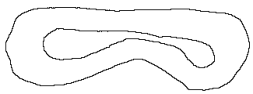
\includegraphics[interpolate=true,width=2.530000in,height=0.940000in]{contents/chapt7/figs/model/mu_paths-img1.png}}%
\end{pgfscope}%
\begin{pgfscope}%
\pgfpathrectangle{\pgfqpoint{2.825000in}{0.508846in}}{\pgfqpoint{2.525000in}{0.932308in}}%
\pgfusepath{clip}%
\pgfsetbuttcap%
\pgfsetroundjoin%
\pgfsetlinewidth{1.505625pt}%
\definecolor{currentstroke}{rgb}{1.000000,0.000000,0.000000}%
\pgfsetstrokecolor{currentstroke}%
\pgfsetdash{{1.500000pt}{2.475000pt}}{0.000000pt}%
\pgfpathmoveto{\pgfqpoint{4.373327in}{1.057765in}}%
\pgfpathlineto{\pgfqpoint{4.373327in}{1.368534in}}%
\pgfusepath{stroke}%
\end{pgfscope}%
\begin{pgfscope}%
\pgfpathrectangle{\pgfqpoint{2.825000in}{0.508846in}}{\pgfqpoint{2.525000in}{0.932308in}}%
\pgfusepath{clip}%
\pgfsetrectcap%
\pgfsetroundjoin%
\pgfsetlinewidth{1.505625pt}%
\definecolor{currentstroke}{rgb}{0.121569,0.466667,0.705882}%
\pgfsetstrokecolor{currentstroke}%
\pgfsetstrokeopacity{0.700000}%
\pgfsetdash{}{0pt}%
\pgfpathmoveto{\pgfqpoint{4.378846in}{1.208077in}}%
\pgfpathlineto{\pgfqpoint{4.319646in}{1.209095in}}%
\pgfpathlineto{\pgfqpoint{4.267847in}{1.212575in}}%
\pgfpathlineto{\pgfqpoint{4.197838in}{1.220133in}}%
\pgfpathlineto{\pgfqpoint{4.131691in}{1.226385in}}%
\pgfpathlineto{\pgfqpoint{4.071268in}{1.229633in}}%
\pgfpathlineto{\pgfqpoint{4.002171in}{1.230940in}}%
\pgfpathlineto{\pgfqpoint{3.893856in}{1.230356in}}%
\pgfpathlineto{\pgfqpoint{3.824040in}{1.227646in}}%
\pgfpathlineto{\pgfqpoint{3.762127in}{1.222814in}}%
\pgfpathlineto{\pgfqpoint{3.692612in}{1.214979in}}%
\pgfpathlineto{\pgfqpoint{3.592659in}{1.201010in}}%
\pgfpathlineto{\pgfqpoint{3.515581in}{1.191401in}}%
\pgfpathlineto{\pgfqpoint{3.453727in}{1.185992in}}%
\pgfpathlineto{\pgfqpoint{3.384313in}{1.179478in}}%
\pgfpathlineto{\pgfqpoint{3.346041in}{1.173709in}}%
\pgfpathlineto{\pgfqpoint{3.315758in}{1.167103in}}%
\pgfpathlineto{\pgfqpoint{3.286001in}{1.158156in}}%
\pgfpathlineto{\pgfqpoint{3.264224in}{1.149694in}}%
\pgfpathlineto{\pgfqpoint{3.243186in}{1.139597in}}%
\pgfpathlineto{\pgfqpoint{3.223103in}{1.127809in}}%
\pgfpathlineto{\pgfqpoint{3.204126in}{1.114259in}}%
\pgfpathlineto{\pgfqpoint{3.186557in}{1.098926in}}%
\pgfpathlineto{\pgfqpoint{3.170618in}{1.081907in}}%
\pgfpathlineto{\pgfqpoint{3.156565in}{1.063341in}}%
\pgfpathlineto{\pgfqpoint{3.144586in}{1.043366in}}%
\pgfpathlineto{\pgfqpoint{3.134878in}{1.022190in}}%
\pgfpathlineto{\pgfqpoint{3.127587in}{1.000090in}}%
\pgfpathlineto{\pgfqpoint{3.122849in}{0.977351in}}%
\pgfpathlineto{\pgfqpoint{3.120726in}{0.954209in}}%
\pgfpathlineto{\pgfqpoint{3.121267in}{0.930937in}}%
\pgfpathlineto{\pgfqpoint{3.124441in}{0.907869in}}%
\pgfpathlineto{\pgfqpoint{3.130212in}{0.885310in}}%
\pgfpathlineto{\pgfqpoint{3.138497in}{0.863533in}}%
\pgfpathlineto{\pgfqpoint{3.149187in}{0.842860in}}%
\pgfpathlineto{\pgfqpoint{3.162105in}{0.823507in}}%
\pgfpathlineto{\pgfqpoint{3.177028in}{0.805639in}}%
\pgfpathlineto{\pgfqpoint{3.193725in}{0.789408in}}%
\pgfpathlineto{\pgfqpoint{3.211990in}{0.774944in}}%
\pgfpathlineto{\pgfqpoint{3.231587in}{0.762331in}}%
\pgfpathlineto{\pgfqpoint{3.252308in}{0.751646in}}%
\pgfpathlineto{\pgfqpoint{3.273878in}{0.742905in}}%
\pgfpathlineto{\pgfqpoint{3.296120in}{0.736095in}}%
\pgfpathlineto{\pgfqpoint{3.318860in}{0.731097in}}%
\pgfpathlineto{\pgfqpoint{3.341936in}{0.727809in}}%
\pgfpathlineto{\pgfqpoint{3.372875in}{0.725964in}}%
\pgfpathlineto{\pgfqpoint{3.403841in}{0.726819in}}%
\pgfpathlineto{\pgfqpoint{3.434680in}{0.730199in}}%
\pgfpathlineto{\pgfqpoint{3.465247in}{0.735880in}}%
\pgfpathlineto{\pgfqpoint{3.502972in}{0.745150in}}%
\pgfpathlineto{\pgfqpoint{3.562652in}{0.762459in}}%
\pgfpathlineto{\pgfqpoint{3.667165in}{0.792595in}}%
\pgfpathlineto{\pgfqpoint{3.967743in}{0.872666in}}%
\pgfpathlineto{\pgfqpoint{4.013210in}{0.882563in}}%
\pgfpathlineto{\pgfqpoint{4.051451in}{0.888869in}}%
\pgfpathlineto{\pgfqpoint{4.089879in}{0.893237in}}%
\pgfpathlineto{\pgfqpoint{4.128598in}{0.895365in}}%
\pgfpathlineto{\pgfqpoint{4.167441in}{0.895126in}}%
\pgfpathlineto{\pgfqpoint{4.206188in}{0.892421in}}%
\pgfpathlineto{\pgfqpoint{4.244709in}{0.887388in}}%
\pgfpathlineto{\pgfqpoint{4.282839in}{0.880139in}}%
\pgfpathlineto{\pgfqpoint{4.320422in}{0.870752in}}%
\pgfpathlineto{\pgfqpoint{4.357358in}{0.859128in}}%
\pgfpathlineto{\pgfqpoint{4.422865in}{0.835129in}}%
\pgfpathlineto{\pgfqpoint{4.481603in}{0.814833in}}%
\pgfpathlineto{\pgfqpoint{4.526352in}{0.801878in}}%
\pgfpathlineto{\pgfqpoint{4.601559in}{0.782781in}}%
\pgfpathlineto{\pgfqpoint{4.677276in}{0.765476in}}%
\pgfpathlineto{\pgfqpoint{4.730788in}{0.755379in}}%
\pgfpathlineto{\pgfqpoint{4.769303in}{0.750208in}}%
\pgfpathlineto{\pgfqpoint{4.808064in}{0.747472in}}%
\pgfpathlineto{\pgfqpoint{4.839138in}{0.747542in}}%
\pgfpathlineto{\pgfqpoint{4.870106in}{0.750029in}}%
\pgfpathlineto{\pgfqpoint{4.893136in}{0.753674in}}%
\pgfpathlineto{\pgfqpoint{4.915836in}{0.758990in}}%
\pgfpathlineto{\pgfqpoint{4.938049in}{0.766053in}}%
\pgfpathlineto{\pgfqpoint{4.959577in}{0.774974in}}%
\pgfpathlineto{\pgfqpoint{4.980161in}{0.785750in}}%
\pgfpathlineto{\pgfqpoint{4.999661in}{0.798401in}}%
\pgfpathlineto{\pgfqpoint{5.017801in}{0.812903in}}%
\pgfpathlineto{\pgfqpoint{5.034312in}{0.829174in}}%
\pgfpathlineto{\pgfqpoint{5.048999in}{0.847091in}}%
\pgfpathlineto{\pgfqpoint{5.061651in}{0.866509in}}%
\pgfpathlineto{\pgfqpoint{5.072121in}{0.887258in}}%
\pgfpathlineto{\pgfqpoint{5.080237in}{0.909053in}}%
\pgfpathlineto{\pgfqpoint{5.085887in}{0.931575in}}%
\pgfpathlineto{\pgfqpoint{5.088917in}{0.954549in}}%
\pgfpathlineto{\pgfqpoint{5.089233in}{0.977707in}}%
\pgfpathlineto{\pgfqpoint{5.086866in}{1.000816in}}%
\pgfpathlineto{\pgfqpoint{5.081860in}{1.023516in}}%
\pgfpathlineto{\pgfqpoint{5.074387in}{1.045491in}}%
\pgfpathlineto{\pgfqpoint{5.064545in}{1.066494in}}%
\pgfpathlineto{\pgfqpoint{5.052464in}{1.086334in}}%
\pgfpathlineto{\pgfqpoint{5.038323in}{1.104786in}}%
\pgfpathlineto{\pgfqpoint{5.022336in}{1.121659in}}%
\pgfpathlineto{\pgfqpoint{5.004708in}{1.136796in}}%
\pgfpathlineto{\pgfqpoint{4.985720in}{1.150117in}}%
\pgfpathlineto{\pgfqpoint{4.965590in}{1.161691in}}%
\pgfpathlineto{\pgfqpoint{4.944540in}{1.171476in}}%
\pgfpathlineto{\pgfqpoint{4.922752in}{1.179514in}}%
\pgfpathlineto{\pgfqpoint{4.892819in}{1.187644in}}%
\pgfpathlineto{\pgfqpoint{4.862297in}{1.193043in}}%
\pgfpathlineto{\pgfqpoint{4.831461in}{1.195870in}}%
\pgfpathlineto{\pgfqpoint{4.792625in}{1.196694in}}%
\pgfpathlineto{\pgfqpoint{4.645122in}{1.196790in}}%
\pgfpathlineto{\pgfqpoint{4.583093in}{1.200692in}}%
\pgfpathlineto{\pgfqpoint{4.505708in}{1.208065in}}%
\pgfpathlineto{\pgfqpoint{4.397500in}{1.219308in}}%
\pgfpathlineto{\pgfqpoint{4.397500in}{1.219308in}}%
\pgfusepath{stroke}%
\end{pgfscope}%
\begin{pgfscope}%
\pgfpathrectangle{\pgfqpoint{2.825000in}{0.508846in}}{\pgfqpoint{2.525000in}{0.932308in}}%
\pgfusepath{clip}%
\pgfsetbuttcap%
\pgfsetroundjoin%
\pgfsetlinewidth{1.505625pt}%
\definecolor{currentstroke}{rgb}{1.000000,0.498039,0.054902}%
\pgfsetstrokecolor{currentstroke}%
\pgfsetstrokeopacity{0.700000}%
\pgfsetdash{{5.550000pt}{2.400000pt}}{0.000000pt}%
\pgfpathmoveto{\pgfqpoint{4.378846in}{1.208077in}}%
\pgfpathlineto{\pgfqpoint{4.300891in}{1.209108in}}%
\pgfpathlineto{\pgfqpoint{4.233472in}{1.212448in}}%
\pgfpathlineto{\pgfqpoint{4.138763in}{1.219795in}}%
\pgfpathlineto{\pgfqpoint{3.986813in}{1.231944in}}%
\pgfpathlineto{\pgfqpoint{3.909472in}{1.235739in}}%
\pgfpathlineto{\pgfqpoint{3.839684in}{1.236909in}}%
\pgfpathlineto{\pgfqpoint{3.769768in}{1.235870in}}%
\pgfpathlineto{\pgfqpoint{3.707726in}{1.232876in}}%
\pgfpathlineto{\pgfqpoint{3.645735in}{1.227812in}}%
\pgfpathlineto{\pgfqpoint{3.576399in}{1.219739in}}%
\pgfpathlineto{\pgfqpoint{3.507376in}{1.209416in}}%
\pgfpathlineto{\pgfqpoint{3.430862in}{1.195710in}}%
\pgfpathlineto{\pgfqpoint{3.369978in}{1.182866in}}%
\pgfpathlineto{\pgfqpoint{3.317389in}{1.169398in}}%
\pgfpathlineto{\pgfqpoint{3.280349in}{1.157800in}}%
\pgfpathlineto{\pgfqpoint{3.244064in}{1.143890in}}%
\pgfpathlineto{\pgfqpoint{3.215910in}{1.130737in}}%
\pgfpathlineto{\pgfqpoint{3.188847in}{1.115486in}}%
\pgfpathlineto{\pgfqpoint{3.163245in}{1.097993in}}%
\pgfpathlineto{\pgfqpoint{3.145184in}{1.083297in}}%
\pgfpathlineto{\pgfqpoint{3.128329in}{1.067281in}}%
\pgfpathlineto{\pgfqpoint{3.112821in}{1.049896in}}%
\pgfpathlineto{\pgfqpoint{3.098906in}{1.031256in}}%
\pgfpathlineto{\pgfqpoint{3.086743in}{1.011461in}}%
\pgfpathlineto{\pgfqpoint{3.076454in}{0.990577in}}%
\pgfpathlineto{\pgfqpoint{3.068138in}{0.968838in}}%
\pgfpathlineto{\pgfqpoint{3.061926in}{0.946378in}}%
\pgfpathlineto{\pgfqpoint{3.057908in}{0.923432in}}%
\pgfpathlineto{\pgfqpoint{3.056125in}{0.900179in}}%
\pgfpathlineto{\pgfqpoint{3.056607in}{0.876868in}}%
\pgfpathlineto{\pgfqpoint{3.059344in}{0.853727in}}%
\pgfpathlineto{\pgfqpoint{3.064249in}{0.830947in}}%
\pgfpathlineto{\pgfqpoint{3.071239in}{0.808722in}}%
\pgfpathlineto{\pgfqpoint{3.080224in}{0.787283in}}%
\pgfpathlineto{\pgfqpoint{3.091113in}{0.766757in}}%
\pgfpathlineto{\pgfqpoint{3.103819in}{0.747303in}}%
\pgfpathlineto{\pgfqpoint{3.118268in}{0.729023in}}%
\pgfpathlineto{\pgfqpoint{3.134264in}{0.712094in}}%
\pgfpathlineto{\pgfqpoint{3.151650in}{0.696531in}}%
\pgfpathlineto{\pgfqpoint{3.170207in}{0.682396in}}%
\pgfpathlineto{\pgfqpoint{3.189775in}{0.669752in}}%
\pgfpathlineto{\pgfqpoint{3.210229in}{0.658658in}}%
\pgfpathlineto{\pgfqpoint{3.231488in}{0.649129in}}%
\pgfpathlineto{\pgfqpoint{3.253394in}{0.641174in}}%
\pgfpathlineto{\pgfqpoint{3.283365in}{0.632997in}}%
\pgfpathlineto{\pgfqpoint{3.313903in}{0.627457in}}%
\pgfpathlineto{\pgfqpoint{3.344823in}{0.624491in}}%
\pgfpathlineto{\pgfqpoint{3.375889in}{0.624007in}}%
\pgfpathlineto{\pgfqpoint{3.406903in}{0.625935in}}%
\pgfpathlineto{\pgfqpoint{3.437711in}{0.630121in}}%
\pgfpathlineto{\pgfqpoint{3.475776in}{0.637892in}}%
\pgfpathlineto{\pgfqpoint{3.513220in}{0.647989in}}%
\pgfpathlineto{\pgfqpoint{3.557517in}{0.662530in}}%
\pgfpathlineto{\pgfqpoint{3.623064in}{0.686965in}}%
\pgfpathlineto{\pgfqpoint{3.746778in}{0.733461in}}%
\pgfpathlineto{\pgfqpoint{3.892398in}{0.787390in}}%
\pgfpathlineto{\pgfqpoint{3.971432in}{0.819561in}}%
\pgfpathlineto{\pgfqpoint{4.064948in}{0.857651in}}%
\pgfpathlineto{\pgfqpoint{4.108818in}{0.873271in}}%
\pgfpathlineto{\pgfqpoint{4.146042in}{0.884470in}}%
\pgfpathlineto{\pgfqpoint{4.183769in}{0.893588in}}%
\pgfpathlineto{\pgfqpoint{4.221974in}{0.900272in}}%
\pgfpathlineto{\pgfqpoint{4.252802in}{0.903687in}}%
\pgfpathlineto{\pgfqpoint{4.283777in}{0.905214in}}%
\pgfpathlineto{\pgfqpoint{4.314784in}{0.904799in}}%
\pgfpathlineto{\pgfqpoint{4.345762in}{0.902479in}}%
\pgfpathlineto{\pgfqpoint{4.376509in}{0.898212in}}%
\pgfpathlineto{\pgfqpoint{4.406889in}{0.892017in}}%
\pgfpathlineto{\pgfqpoint{4.436835in}{0.883911in}}%
\pgfpathlineto{\pgfqpoint{4.466181in}{0.873909in}}%
\pgfpathlineto{\pgfqpoint{4.501997in}{0.859213in}}%
\pgfpathlineto{\pgfqpoint{4.543911in}{0.839348in}}%
\pgfpathlineto{\pgfqpoint{4.605618in}{0.806937in}}%
\pgfpathlineto{\pgfqpoint{4.674393in}{0.771106in}}%
\pgfpathlineto{\pgfqpoint{4.716690in}{0.751624in}}%
\pgfpathlineto{\pgfqpoint{4.752819in}{0.737363in}}%
\pgfpathlineto{\pgfqpoint{4.789710in}{0.725516in}}%
\pgfpathlineto{\pgfqpoint{4.819877in}{0.718070in}}%
\pgfpathlineto{\pgfqpoint{4.850505in}{0.712753in}}%
\pgfpathlineto{\pgfqpoint{4.881404in}{0.709800in}}%
\pgfpathlineto{\pgfqpoint{4.912422in}{0.709438in}}%
\pgfpathlineto{\pgfqpoint{4.943261in}{0.711877in}}%
\pgfpathlineto{\pgfqpoint{4.966098in}{0.715636in}}%
\pgfpathlineto{\pgfqpoint{4.988578in}{0.721115in}}%
\pgfpathlineto{\pgfqpoint{5.010559in}{0.728332in}}%
\pgfpathlineto{\pgfqpoint{5.031910in}{0.737305in}}%
\pgfpathlineto{\pgfqpoint{5.052495in}{0.747983in}}%
\pgfpathlineto{\pgfqpoint{5.072127in}{0.760277in}}%
\pgfpathlineto{\pgfqpoint{5.090666in}{0.774165in}}%
\pgfpathlineto{\pgfqpoint{5.108036in}{0.789608in}}%
\pgfpathlineto{\pgfqpoint{5.124045in}{0.806428in}}%
\pgfpathlineto{\pgfqpoint{5.138552in}{0.824528in}}%
\pgfpathlineto{\pgfqpoint{5.151449in}{0.843812in}}%
\pgfpathlineto{\pgfqpoint{5.162690in}{0.864083in}}%
\pgfpathlineto{\pgfqpoint{5.172192in}{0.885221in}}%
\pgfpathlineto{\pgfqpoint{5.179887in}{0.907104in}}%
\pgfpathlineto{\pgfqpoint{5.185685in}{0.929567in}}%
\pgfpathlineto{\pgfqpoint{5.189558in}{0.952491in}}%
\pgfpathlineto{\pgfqpoint{5.191491in}{0.975685in}}%
\pgfpathlineto{\pgfqpoint{5.191482in}{0.998999in}}%
\pgfpathlineto{\pgfqpoint{5.189578in}{1.022240in}}%
\pgfpathlineto{\pgfqpoint{5.185802in}{1.045248in}}%
\pgfpathlineto{\pgfqpoint{5.180187in}{1.067861in}}%
\pgfpathlineto{\pgfqpoint{5.172727in}{1.089961in}}%
\pgfpathlineto{\pgfqpoint{5.163495in}{1.111352in}}%
\pgfpathlineto{\pgfqpoint{5.152544in}{1.131896in}}%
\pgfpathlineto{\pgfqpoint{5.139961in}{1.151494in}}%
\pgfpathlineto{\pgfqpoint{5.125876in}{1.170044in}}%
\pgfpathlineto{\pgfqpoint{5.110371in}{1.187449in}}%
\pgfpathlineto{\pgfqpoint{5.093573in}{1.203590in}}%
\pgfpathlineto{\pgfqpoint{5.075573in}{1.218357in}}%
\pgfpathlineto{\pgfqpoint{5.056477in}{1.231693in}}%
\pgfpathlineto{\pgfqpoint{5.036418in}{1.243534in}}%
\pgfpathlineto{\pgfqpoint{5.008452in}{1.257107in}}%
\pgfpathlineto{\pgfqpoint{4.979451in}{1.268172in}}%
\pgfpathlineto{\pgfqpoint{4.949575in}{1.276797in}}%
\pgfpathlineto{\pgfqpoint{4.919159in}{1.283083in}}%
\pgfpathlineto{\pgfqpoint{4.888336in}{1.287165in}}%
\pgfpathlineto{\pgfqpoint{4.849570in}{1.289548in}}%
\pgfpathlineto{\pgfqpoint{4.802983in}{1.289683in}}%
\pgfpathlineto{\pgfqpoint{4.740970in}{1.287211in}}%
\pgfpathlineto{\pgfqpoint{4.593371in}{1.280502in}}%
\pgfpathlineto{\pgfqpoint{4.445789in}{1.277692in}}%
\pgfpathlineto{\pgfqpoint{4.445789in}{1.277692in}}%
\pgfusepath{stroke}%
\end{pgfscope}%
\begin{pgfscope}%
\pgfpathrectangle{\pgfqpoint{2.825000in}{0.508846in}}{\pgfqpoint{2.525000in}{0.932308in}}%
\pgfusepath{clip}%
\pgfsetbuttcap%
\pgfsetroundjoin%
\pgfsetlinewidth{1.505625pt}%
\definecolor{currentstroke}{rgb}{0.172549,0.627451,0.172549}%
\pgfsetstrokecolor{currentstroke}%
\pgfsetstrokeopacity{0.700000}%
\pgfsetdash{{5.550000pt}{2.400000pt}}{0.000000pt}%
\pgfpathmoveto{\pgfqpoint{4.378846in}{1.208077in}}%
\pgfpathlineto{\pgfqpoint{4.319631in}{1.209092in}}%
\pgfpathlineto{\pgfqpoint{4.267827in}{1.212289in}}%
\pgfpathlineto{\pgfqpoint{4.204646in}{1.218619in}}%
\pgfpathlineto{\pgfqpoint{4.093565in}{1.229755in}}%
\pgfpathlineto{\pgfqpoint{4.032774in}{1.233359in}}%
\pgfpathlineto{\pgfqpoint{3.963667in}{1.235093in}}%
\pgfpathlineto{\pgfqpoint{3.894161in}{1.234641in}}%
\pgfpathlineto{\pgfqpoint{3.832163in}{1.231988in}}%
\pgfpathlineto{\pgfqpoint{3.762468in}{1.226567in}}%
\pgfpathlineto{\pgfqpoint{3.685262in}{1.218196in}}%
\pgfpathlineto{\pgfqpoint{3.592922in}{1.205749in}}%
\pgfpathlineto{\pgfqpoint{3.500843in}{1.191018in}}%
\pgfpathlineto{\pgfqpoint{3.378308in}{1.170798in}}%
\pgfpathlineto{\pgfqpoint{3.293970in}{1.157206in}}%
\pgfpathlineto{\pgfqpoint{3.263721in}{1.150102in}}%
\pgfpathlineto{\pgfqpoint{3.241465in}{1.143113in}}%
\pgfpathlineto{\pgfqpoint{3.219815in}{1.134403in}}%
\pgfpathlineto{\pgfqpoint{3.199053in}{1.123771in}}%
\pgfpathlineto{\pgfqpoint{3.179509in}{1.111089in}}%
\pgfpathlineto{\pgfqpoint{3.161515in}{1.096359in}}%
\pgfpathlineto{\pgfqpoint{3.145350in}{1.079644in}}%
\pgfpathlineto{\pgfqpoint{3.131234in}{1.061147in}}%
\pgfpathlineto{\pgfqpoint{3.119378in}{1.041117in}}%
\pgfpathlineto{\pgfqpoint{3.109967in}{1.019857in}}%
\pgfpathlineto{\pgfqpoint{3.103116in}{0.997706in}}%
\pgfpathlineto{\pgfqpoint{3.098919in}{0.974907in}}%
\pgfpathlineto{\pgfqpoint{3.097405in}{0.951740in}}%
\pgfpathlineto{\pgfqpoint{3.098583in}{0.928484in}}%
\pgfpathlineto{\pgfqpoint{3.102387in}{0.905507in}}%
\pgfpathlineto{\pgfqpoint{3.108763in}{0.883104in}}%
\pgfpathlineto{\pgfqpoint{3.117618in}{0.861548in}}%
\pgfpathlineto{\pgfqpoint{3.128823in}{0.841123in}}%
\pgfpathlineto{\pgfqpoint{3.142092in}{0.821999in}}%
\pgfpathlineto{\pgfqpoint{3.157256in}{0.804388in}}%
\pgfpathlineto{\pgfqpoint{3.174136in}{0.788406in}}%
\pgfpathlineto{\pgfqpoint{3.192566in}{0.774136in}}%
\pgfpathlineto{\pgfqpoint{3.212236in}{0.761708in}}%
\pgfpathlineto{\pgfqpoint{3.232988in}{0.751185in}}%
\pgfpathlineto{\pgfqpoint{3.254638in}{0.742530in}}%
\pgfpathlineto{\pgfqpoint{3.276888in}{0.735598in}}%
\pgfpathlineto{\pgfqpoint{3.299599in}{0.730361in}}%
\pgfpathlineto{\pgfqpoint{3.330352in}{0.725868in}}%
\pgfpathlineto{\pgfqpoint{3.361385in}{0.724036in}}%
\pgfpathlineto{\pgfqpoint{3.392428in}{0.724698in}}%
\pgfpathlineto{\pgfqpoint{3.423300in}{0.727581in}}%
\pgfpathlineto{\pgfqpoint{3.461648in}{0.733299in}}%
\pgfpathlineto{\pgfqpoint{3.514984in}{0.743790in}}%
\pgfpathlineto{\pgfqpoint{3.598186in}{0.762744in}}%
\pgfpathlineto{\pgfqpoint{3.695934in}{0.787218in}}%
\pgfpathlineto{\pgfqpoint{3.785765in}{0.811941in}}%
\pgfpathlineto{\pgfqpoint{3.890008in}{0.843127in}}%
\pgfpathlineto{\pgfqpoint{3.949713in}{0.859963in}}%
\pgfpathlineto{\pgfqpoint{3.994929in}{0.870714in}}%
\pgfpathlineto{\pgfqpoint{4.040728in}{0.879250in}}%
\pgfpathlineto{\pgfqpoint{4.079261in}{0.884427in}}%
\pgfpathlineto{\pgfqpoint{4.117972in}{0.887509in}}%
\pgfpathlineto{\pgfqpoint{4.156747in}{0.888282in}}%
\pgfpathlineto{\pgfqpoint{4.195584in}{0.886722in}}%
\pgfpathlineto{\pgfqpoint{4.234165in}{0.882931in}}%
\pgfpathlineto{\pgfqpoint{4.272531in}{0.876927in}}%
\pgfpathlineto{\pgfqpoint{4.310448in}{0.868634in}}%
\pgfpathlineto{\pgfqpoint{4.362839in}{0.854230in}}%
\pgfpathlineto{\pgfqpoint{4.430263in}{0.835926in}}%
\pgfpathlineto{\pgfqpoint{4.475830in}{0.826102in}}%
\pgfpathlineto{\pgfqpoint{4.574778in}{0.806647in}}%
\pgfpathlineto{\pgfqpoint{4.604472in}{0.797516in}}%
\pgfpathlineto{\pgfqpoint{4.633272in}{0.785931in}}%
\pgfpathlineto{\pgfqpoint{4.661066in}{0.772154in}}%
\pgfpathlineto{\pgfqpoint{4.701469in}{0.748909in}}%
\pgfpathlineto{\pgfqpoint{4.742087in}{0.726012in}}%
\pgfpathlineto{\pgfqpoint{4.770065in}{0.712892in}}%
\pgfpathlineto{\pgfqpoint{4.791629in}{0.704903in}}%
\pgfpathlineto{\pgfqpoint{4.813647in}{0.698818in}}%
\pgfpathlineto{\pgfqpoint{4.836050in}{0.694898in}}%
\pgfpathlineto{\pgfqpoint{4.858631in}{0.693292in}}%
\pgfpathlineto{\pgfqpoint{4.881171in}{0.694088in}}%
\pgfpathlineto{\pgfqpoint{4.903503in}{0.697294in}}%
\pgfpathlineto{\pgfqpoint{4.925514in}{0.702750in}}%
\pgfpathlineto{\pgfqpoint{4.946961in}{0.710275in}}%
\pgfpathlineto{\pgfqpoint{4.967690in}{0.719794in}}%
\pgfpathlineto{\pgfqpoint{4.987547in}{0.731155in}}%
\pgfpathlineto{\pgfqpoint{5.006403in}{0.744245in}}%
\pgfpathlineto{\pgfqpoint{5.024067in}{0.759007in}}%
\pgfpathlineto{\pgfqpoint{5.040376in}{0.775305in}}%
\pgfpathlineto{\pgfqpoint{5.055236in}{0.792992in}}%
\pgfpathlineto{\pgfqpoint{5.068505in}{0.811970in}}%
\pgfpathlineto{\pgfqpoint{5.079995in}{0.832117in}}%
\pgfpathlineto{\pgfqpoint{5.089558in}{0.853231in}}%
\pgfpathlineto{\pgfqpoint{5.097115in}{0.875213in}}%
\pgfpathlineto{\pgfqpoint{5.102540in}{0.897848in}}%
\pgfpathlineto{\pgfqpoint{5.105772in}{0.920937in}}%
\pgfpathlineto{\pgfqpoint{5.106738in}{0.944218in}}%
\pgfpathlineto{\pgfqpoint{5.105416in}{0.967444in}}%
\pgfpathlineto{\pgfqpoint{5.101722in}{0.990447in}}%
\pgfpathlineto{\pgfqpoint{5.095627in}{1.012931in}}%
\pgfpathlineto{\pgfqpoint{5.087231in}{1.034650in}}%
\pgfpathlineto{\pgfqpoint{5.076621in}{1.055407in}}%
\pgfpathlineto{\pgfqpoint{5.063924in}{1.074957in}}%
\pgfpathlineto{\pgfqpoint{5.049348in}{1.093143in}}%
\pgfpathlineto{\pgfqpoint{5.033071in}{1.109799in}}%
\pgfpathlineto{\pgfqpoint{5.015263in}{1.124791in}}%
\pgfpathlineto{\pgfqpoint{4.996133in}{1.138010in}}%
\pgfpathlineto{\pgfqpoint{4.975881in}{1.149454in}}%
\pgfpathlineto{\pgfqpoint{4.954738in}{1.159076in}}%
\pgfpathlineto{\pgfqpoint{4.925497in}{1.169472in}}%
\pgfpathlineto{\pgfqpoint{4.895546in}{1.177540in}}%
\pgfpathlineto{\pgfqpoint{4.857525in}{1.184937in}}%
\pgfpathlineto{\pgfqpoint{4.819107in}{1.190081in}}%
\pgfpathlineto{\pgfqpoint{4.757191in}{1.195735in}}%
\pgfpathlineto{\pgfqpoint{4.377753in}{1.224060in}}%
\pgfpathlineto{\pgfqpoint{4.377753in}{1.224060in}}%
\pgfusepath{stroke}%
\end{pgfscope}%
\begin{pgfscope}%
\definecolor{textcolor}{rgb}{0.000000,0.000000,0.000000}%
\pgfsetstrokecolor{textcolor}%
\pgfsetfillcolor{textcolor}%
\pgftext[x=4.087500in,y=1.524487in,,base]{\color{textcolor}\rmfamily\fontsize{12.000000}{14.400000}\selectfont Steering and velocity control}%
\end{pgfscope}%
\begin{pgfscope}%
\pgfsetbuttcap%
\pgfsetmiterjoin%
\definecolor{currentfill}{rgb}{1.000000,1.000000,1.000000}%
\pgfsetfillcolor{currentfill}%
\pgfsetfillopacity{0.800000}%
\pgfsetlinewidth{1.003750pt}%
\definecolor{currentstroke}{rgb}{0.800000,0.800000,0.800000}%
\pgfsetstrokecolor{currentstroke}%
\pgfsetstrokeopacity{0.800000}%
\pgfsetdash{}{0pt}%
\pgfpathmoveto{\pgfqpoint{0.494025in}{0.069444in}}%
\pgfpathlineto{\pgfqpoint{5.005975in}{0.069444in}}%
\pgfpathquadraticcurveto{\pgfqpoint{5.033752in}{0.069444in}}{\pgfqpoint{5.033752in}{0.097222in}}%
\pgfpathlineto{\pgfqpoint{5.033752in}{0.289157in}}%
\pgfpathquadraticcurveto{\pgfqpoint{5.033752in}{0.316935in}}{\pgfqpoint{5.005975in}{0.316935in}}%
\pgfpathlineto{\pgfqpoint{0.494025in}{0.316935in}}%
\pgfpathquadraticcurveto{\pgfqpoint{0.466248in}{0.316935in}}{\pgfqpoint{0.466248in}{0.289157in}}%
\pgfpathlineto{\pgfqpoint{0.466248in}{0.097222in}}%
\pgfpathquadraticcurveto{\pgfqpoint{0.466248in}{0.069444in}}{\pgfqpoint{0.494025in}{0.069444in}}%
\pgfpathlineto{\pgfqpoint{0.494025in}{0.069444in}}%
\pgfpathclose%
\pgfusepath{stroke,fill}%
\end{pgfscope}%
\begin{pgfscope}%
\pgfsetrectcap%
\pgfsetroundjoin%
\pgfsetlinewidth{1.505625pt}%
\definecolor{currentstroke}{rgb}{0.121569,0.466667,0.705882}%
\pgfsetstrokecolor{currentstroke}%
\pgfsetstrokeopacity{0.700000}%
\pgfsetdash{}{0pt}%
\pgfpathmoveto{\pgfqpoint{0.521803in}{0.204467in}}%
\pgfpathlineto{\pgfqpoint{0.660692in}{0.204467in}}%
\pgfpathlineto{\pgfqpoint{0.799581in}{0.204467in}}%
\pgfusepath{stroke}%
\end{pgfscope}%
\begin{pgfscope}%
\definecolor{textcolor}{rgb}{0.000000,0.000000,0.000000}%
\pgfsetstrokecolor{textcolor}%
\pgfsetfillcolor{textcolor}%
\pgftext[x=0.910692in,y=0.155856in,left,base]{\color{textcolor}\rmfamily\fontsize{10.000000}{12.000000}\selectfont No model error}%
\end{pgfscope}%
\begin{pgfscope}%
\pgfsetbuttcap%
\pgfsetroundjoin%
\pgfsetlinewidth{1.505625pt}%
\definecolor{currentstroke}{rgb}{1.000000,0.498039,0.054902}%
\pgfsetstrokecolor{currentstroke}%
\pgfsetstrokeopacity{0.700000}%
\pgfsetdash{{5.550000pt}{2.400000pt}}{0.000000pt}%
\pgfpathmoveto{\pgfqpoint{2.277744in}{0.204467in}}%
\pgfpathlineto{\pgfqpoint{2.416633in}{0.204467in}}%
\pgfpathlineto{\pgfqpoint{2.555522in}{0.204467in}}%
\pgfusepath{stroke}%
\end{pgfscope}%
\begin{pgfscope}%
\definecolor{textcolor}{rgb}{0.000000,0.000000,0.000000}%
\pgfsetstrokecolor{textcolor}%
\pgfsetfillcolor{textcolor}%
\pgftext[x=2.666633in,y=0.155856in,left,base]{\color{textcolor}\rmfamily\fontsize{10.000000}{12.000000}\selectfont Wet asphalt}%
\end{pgfscope}%
\begin{pgfscope}%
\pgfsetbuttcap%
\pgfsetroundjoin%
\pgfsetlinewidth{1.505625pt}%
\definecolor{currentstroke}{rgb}{0.172549,0.627451,0.172549}%
\pgfsetstrokecolor{currentstroke}%
\pgfsetstrokeopacity{0.700000}%
\pgfsetdash{{5.550000pt}{2.400000pt}}{0.000000pt}%
\pgfpathmoveto{\pgfqpoint{3.773471in}{0.204467in}}%
\pgfpathlineto{\pgfqpoint{3.912360in}{0.204467in}}%
\pgfpathlineto{\pgfqpoint{4.051249in}{0.204467in}}%
\pgfusepath{stroke}%
\end{pgfscope}%
\begin{pgfscope}%
\definecolor{textcolor}{rgb}{0.000000,0.000000,0.000000}%
\pgfsetstrokecolor{textcolor}%
\pgfsetfillcolor{textcolor}%
\pgftext[x=4.162360in,y=0.155856in,left,base]{\color{textcolor}\rmfamily\fontsize{10.000000}{12.000000}\selectfont Dry asphalt}%
\end{pgfscope}%
\end{pgfpicture}%
\makeatother%
\endgroup%

    \caption[]{}
    \label{fig:mu_wet_gravel_path}
\end{figure}


\section{Summary}

In this chapter, we compared the performance of end-to-end and partial end-to-end agents under conditions where uncertainties associated with deployment in the real-world were present.
We first addressed the issue of observation uncertainty by measuring the performance of agents when there was noise present in the observation vector.
Both the end-to-end and partial end-to-end systems were fairly robust to noise.
While the performance of the end-to-end system did decreased slightly when noise was present in the observation, the partial end-to-end system was not negatively affected.
Furthermore, the rate of lap completion under test conditions for agents trained with and without noise in the observation vector was the same.


We then compared the performance of our partial end-to-end solution to the end-to-end baseline under conditions where the vehicle model was mismatched.
The scenarios that we considered were (a) a mismatch in mass, (b) tire cornering stiffness coefficient, and (c) road surface friction coefficient.
In all three of these cases, our partial end-to-end proved more robust to model mismatches than the end-to-end agent.

We observed that the end-to-end baseline tended to exhibit erratic and dangerous slaloming behaviour, and also selected extreme control actions when model mismatches were present.
Experiments with the end-to-end agent were also not repeatable, as it exhibited slightly different behaviour on every lap.
However, our partial end-to-end solution mitigated the effect of model-mismatches by decoupling planning from control.
The feedback steering controller outputs smooth steering controls at a fast rate, which results in good path tracking behaviour and prevents the vehicle from slaloming.
Furthermore, our partial end-to-end solution performed laps that were repeatable.



